% Full instructions available at:
% https://github.com/elauksap/focus-beamertheme

\documentclass{beamer}
\usetheme[numbering=progressbar]{focus}
\usepackage{tikz}
\usetikzlibrary{positioning}
\usetikzlibrary{shapes,arrows}
\usepackage{transparent}
\usepackage{fancyvrb}
\usepackage{listings}
\usepackage{tabularx}
\usepackage{amsfonts}
\usepackage{csquotes}
\definecolor{main}{RGB}{47, 161, 219}
\definecolor{background}{RGB}{240, 247, 255}
\definecolor{textcolor}{RGB}{85, 87, 83}

\title{D4 Project}
\subtitle{Open and collaborative network monitoring}
\author{Jean-Louis Huynen}
\titlegraphic{
\includegraphics[scale=0.20]{../../logos/d4-logo.pdf}}
\institute{Team CIRCL \\ \url{https://www.d4-project.org/}}
\date{2019/05/21}

\begin{document}
    \begin{frame}
        \maketitle
    \end{frame}

\begin{frame}
        \frametitle{Problem statement}
        \begin{itemize}
                \item CSIRTs (or private organisations) build their {\bf own honeypot, honeynet or blackhole monitoring network}
                \item Designing, managing and operating such infrastructure is a tedious and resource intensive task
                \item {\bf Automatic sharing} between monitoring networks from different organisations is missing
                \item Sensors and processing are often seen as blackbox or difficult to audit

        \end{itemize}
\end{frame}


\begin{frame}
 \frametitle{Objective}
 \begin{itemize}
         \item Based on our experience with
           MISP\footnote{\url{https://github.com/MISP/MISP}} where sharing
           played an important role, we transpose the model in D4 project
         \item Keeping the protocol and code base {\bf simple and minimal}
         \item Allowing every organisation to {\bf control and audit their own sensor network}
         \item Extending D4 or {\bf encapsulating legacy monitoring protocols} must be as simple as possible
         \item Ensuring that the sensor server has {\bf no control on the sensor} (unidirectional streaming)
         \item Don't force users to use dedicated sensors and allow {\bf flexibility of sensor support} (software, hardware, virtual)

 \end{itemize}
\end{frame}


\begin{frame}
        \frametitle{(short) History}
 \begin{itemize}
        \item D4 Project (co-funded under INEA CEF EU program) started - {\bf 1st November 2018}
        \item D4 encapsulation protocol version 1 published  - {\bf 1st December 2018}
        \item v0.1 release of the D4 core\footnote{\url{https://www.github.com/D4-project/d4-core}} including a server and simple D4 C client - {\bf 21st January 2019}
        \item First version of a golang D4
          client\footnote{\url{https://www.github.com/D4-project/d4-goclient/}}
          running on ARM, MIPS, PPC and x86 - {\bf 14th February 2019}
 \end{itemize}
\end{frame}

\begin{frame}
        \frametitle{(short) History}
\begin{center}
  \begin{tabularx}{\linewidth}%
    {>{\setlength\hsize{0.6\hsize}\raggedright}X%
     >{\setlength\hsize{0.4\hsize}\raggedright}X}

\hline
Release                          & Date \tabularnewline
\hline
analyzer-d4-passivedns-v0.1      & Apr. 5,  2019 \tabularnewline
analyzer-d4-passivessl-0.1       & Apr. 25, 2019 \tabularnewline
analyzer-d4-pibs-v0.1            & Apr. 8, 2019  \tabularnewline
BGP-Ranking-1.0                  & Apr. 25, 2019 \tabularnewline
d4-core-v0.1                     & Jan. 25, 2019 \tabularnewline
d4-core-v0.2                     & Feb. 14, 2019 \tabularnewline
d4-core-v0.3                     & Apr. 8, 2019  \tabularnewline
d4-goclient-v0.1                 & Feb. 14, 2019 \tabularnewline
d4-goclient-v0.2                 & Apr. 8, 2019  \tabularnewline
d4-server-packer-0.1             & Apr. 25, 2019 \tabularnewline
IPASN-History-1.0                & Apr. 25, 2019 \tabularnewline
sensor-d4-tls-fingerprinting-0.1 & Apr. 25, 2019 \tabularnewline
\hline

\end{tabularx}
\end{center}

see \url{https://github.com/D4-Project}
\end{frame}

\begin{frame}
\frametitle{D4 Overview}
        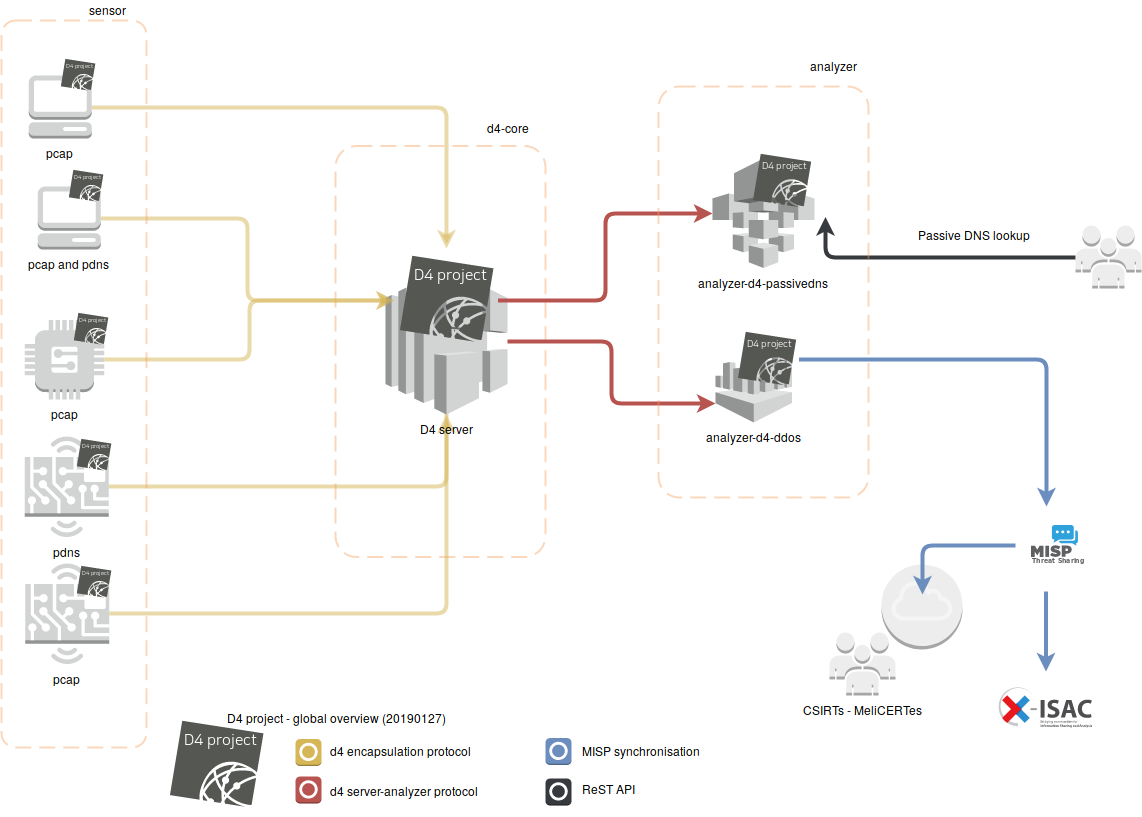
\includegraphics[scale=0.38]{../../diagram/d4-overview.png}
\end{frame}

\begin{frame}
        \frametitle{Roadmap - output}

                 CIRCL will host a server instance for organisations willing to
                  contribute to a public dataset without running their own D4 server:
                  \begin{itemize}
                  \item [\checkmark]Passive SSL 
                  \item [\checkmark] Passive DNS 
                  \item [\checkmark]Blackhole DDoS
                  \item BGP mapping 
                  \item egress filtering mapping
                  \item Radio-Specturm monitoring: 802.11, BLE, etc. 
                  \item ...
                  \end{itemize}
\end{frame}

\begin{frame}
        \frametitle{D4 encapsulation protocol}
        \includegraphics[scale=0.38]{../../diagram/d4-protocol-encapsulation.png}
\end{frame}

\begin{frame}
    \frametitle{D4 Header}
    \begin{tabular}{|l|l|l|}
        \hline
        Name & 	bit size&  	Description\\
        \hline
        version &	uint 8 &	Version of the header \\
        type 	& uint 8   &	Data encapsulated type\\
        uuid 	& uint 128 & 	Sensor UUID\\
        timestamp &  	uint 64 &	Encapsulation time\\
        hmac 	& uint 256 &	Authentication header (HMAC-SHA-256-128)\\
        size 	& uint 32 	& Payload size\\
        \hline
    \end{tabular}
\end{frame}


\begin{frame}
    \frametitle{D4 Header}
    \framesubtitle{Types}
        \begin{tabular}{|l|l|}
            \hline
            Type &	Description\\
            \hline
            0 	& Reserved\\
            1 	& pcap (libpcap 2.4)\\
            2 	& meta header (JSON)\\
            3 	& generic log line\\
            4 	& dnscap output\\
            5 	& pcapng (diagnostic)\\
            6 	& generic NDJSON or JSON Lines\\
            7 	& generic YAF (Yet Another Flowmeter)\\
            8  	& passivedns CSV stream\\
            254 &	type defined by meta header (type 2)\\
            \hline
        \end{tabular}
\end{frame}

\begin{frame}
    \frametitle{D4 meta header}
    \framesubtitle{Meta types}
        D4 header includes an easy way to {\bf extend the protocol} (via type 2) without altering the format. Within a D4 session, the initial D4 packet(s) type 2 defines
        the custom headers and then the following packets with type 254 is the custom data encapsulated.
    \small
    \begin{lstlisting}
{
  "type": "ja3-jl",
  "encoding": "utf-8",
  "tags": [
    "tlp:white"
  ],
  "misp:org": "5b642239-4db4-4580-adf4-4ebd950d210f"
}
\end{lstlisting}

\end{frame}

\begin{frame}
    \frametitle{D4 server}
   \begin{itemize}
           \item D4 core server\footnote{\url{https://github.com/D4-project/d4-core}} is a complete server to handle clients (sensors) including the decapsulation of the D4 protocol, control of sensor registrations, management of decoding protocols and dispatching to adequate decoders/analysers.
           \item D4 server is written in Python 3.6 and runs on standard GNU/Linux distribution.
   \end{itemize}
\end{frame}

\begin{frame}
        \frametitle{D4 server - management interface}
The D4 server provides a {\bf web interface} to manage D4 sensors, sessions and analyzer.
        \begin{itemize}
\item Get Sensors status, errors and statistics
\item Get all connected sensors
\item Manage Sensors (stream size limit, secret key, ...)
\item Manage Accepted types
\item UUID/IP blocklist
\item  Create Analyzer Queues
        \end{itemize}
\end{frame}

\begin{frame}
        \frametitle{D4 server - main interface}
        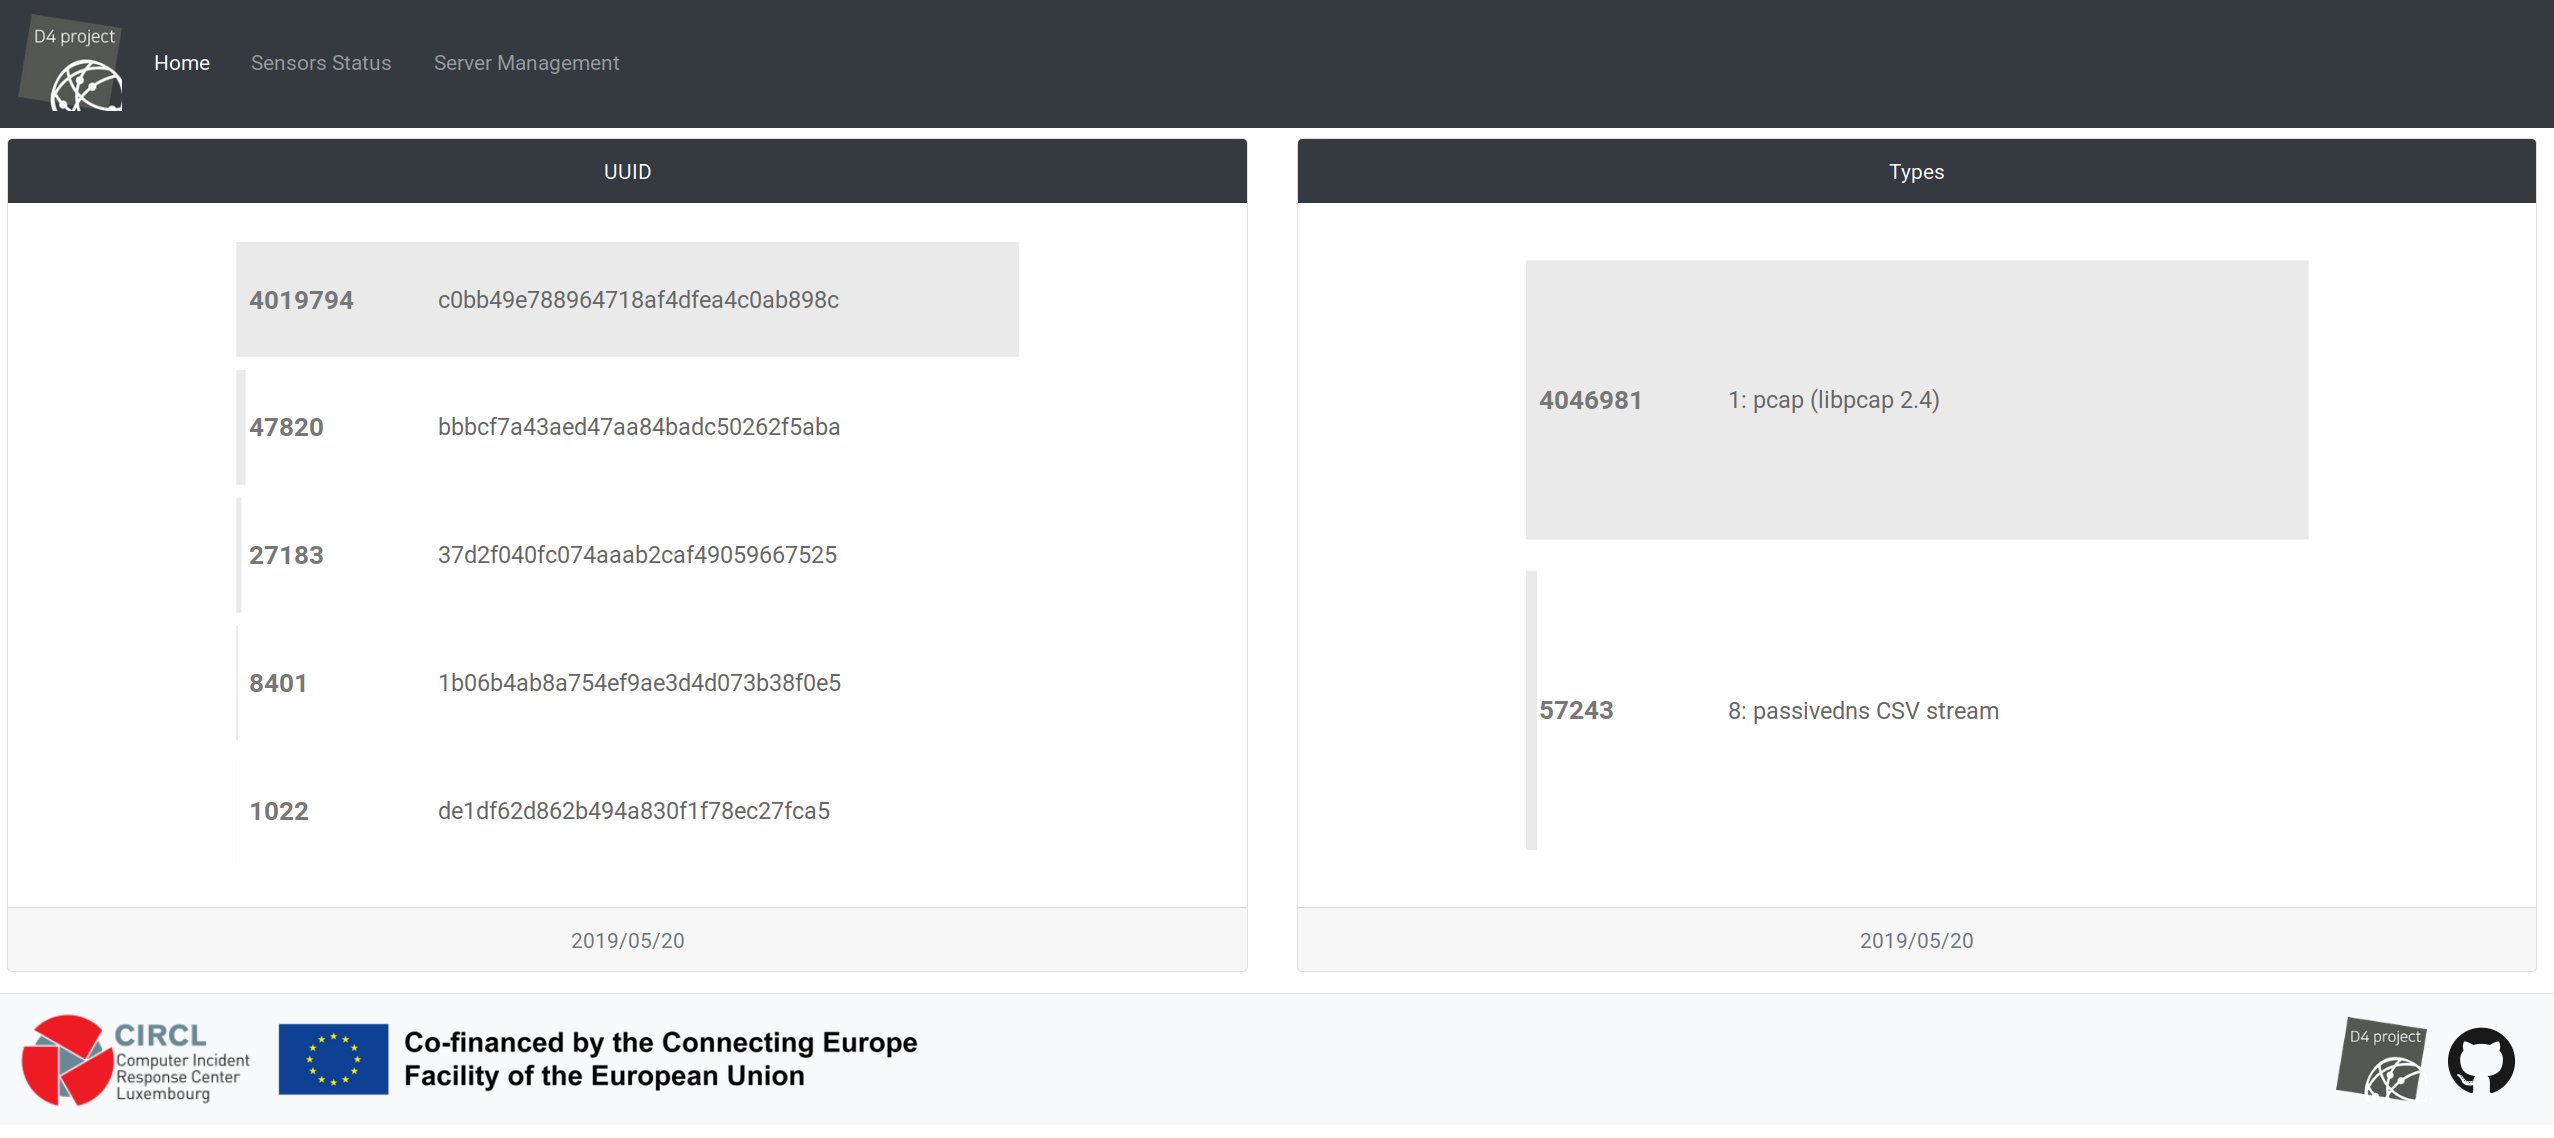
\includegraphics[width=\textwidth]{./d4-5.png}
\end{frame}

\begin{frame}
        \frametitle{D4 server - server management}
        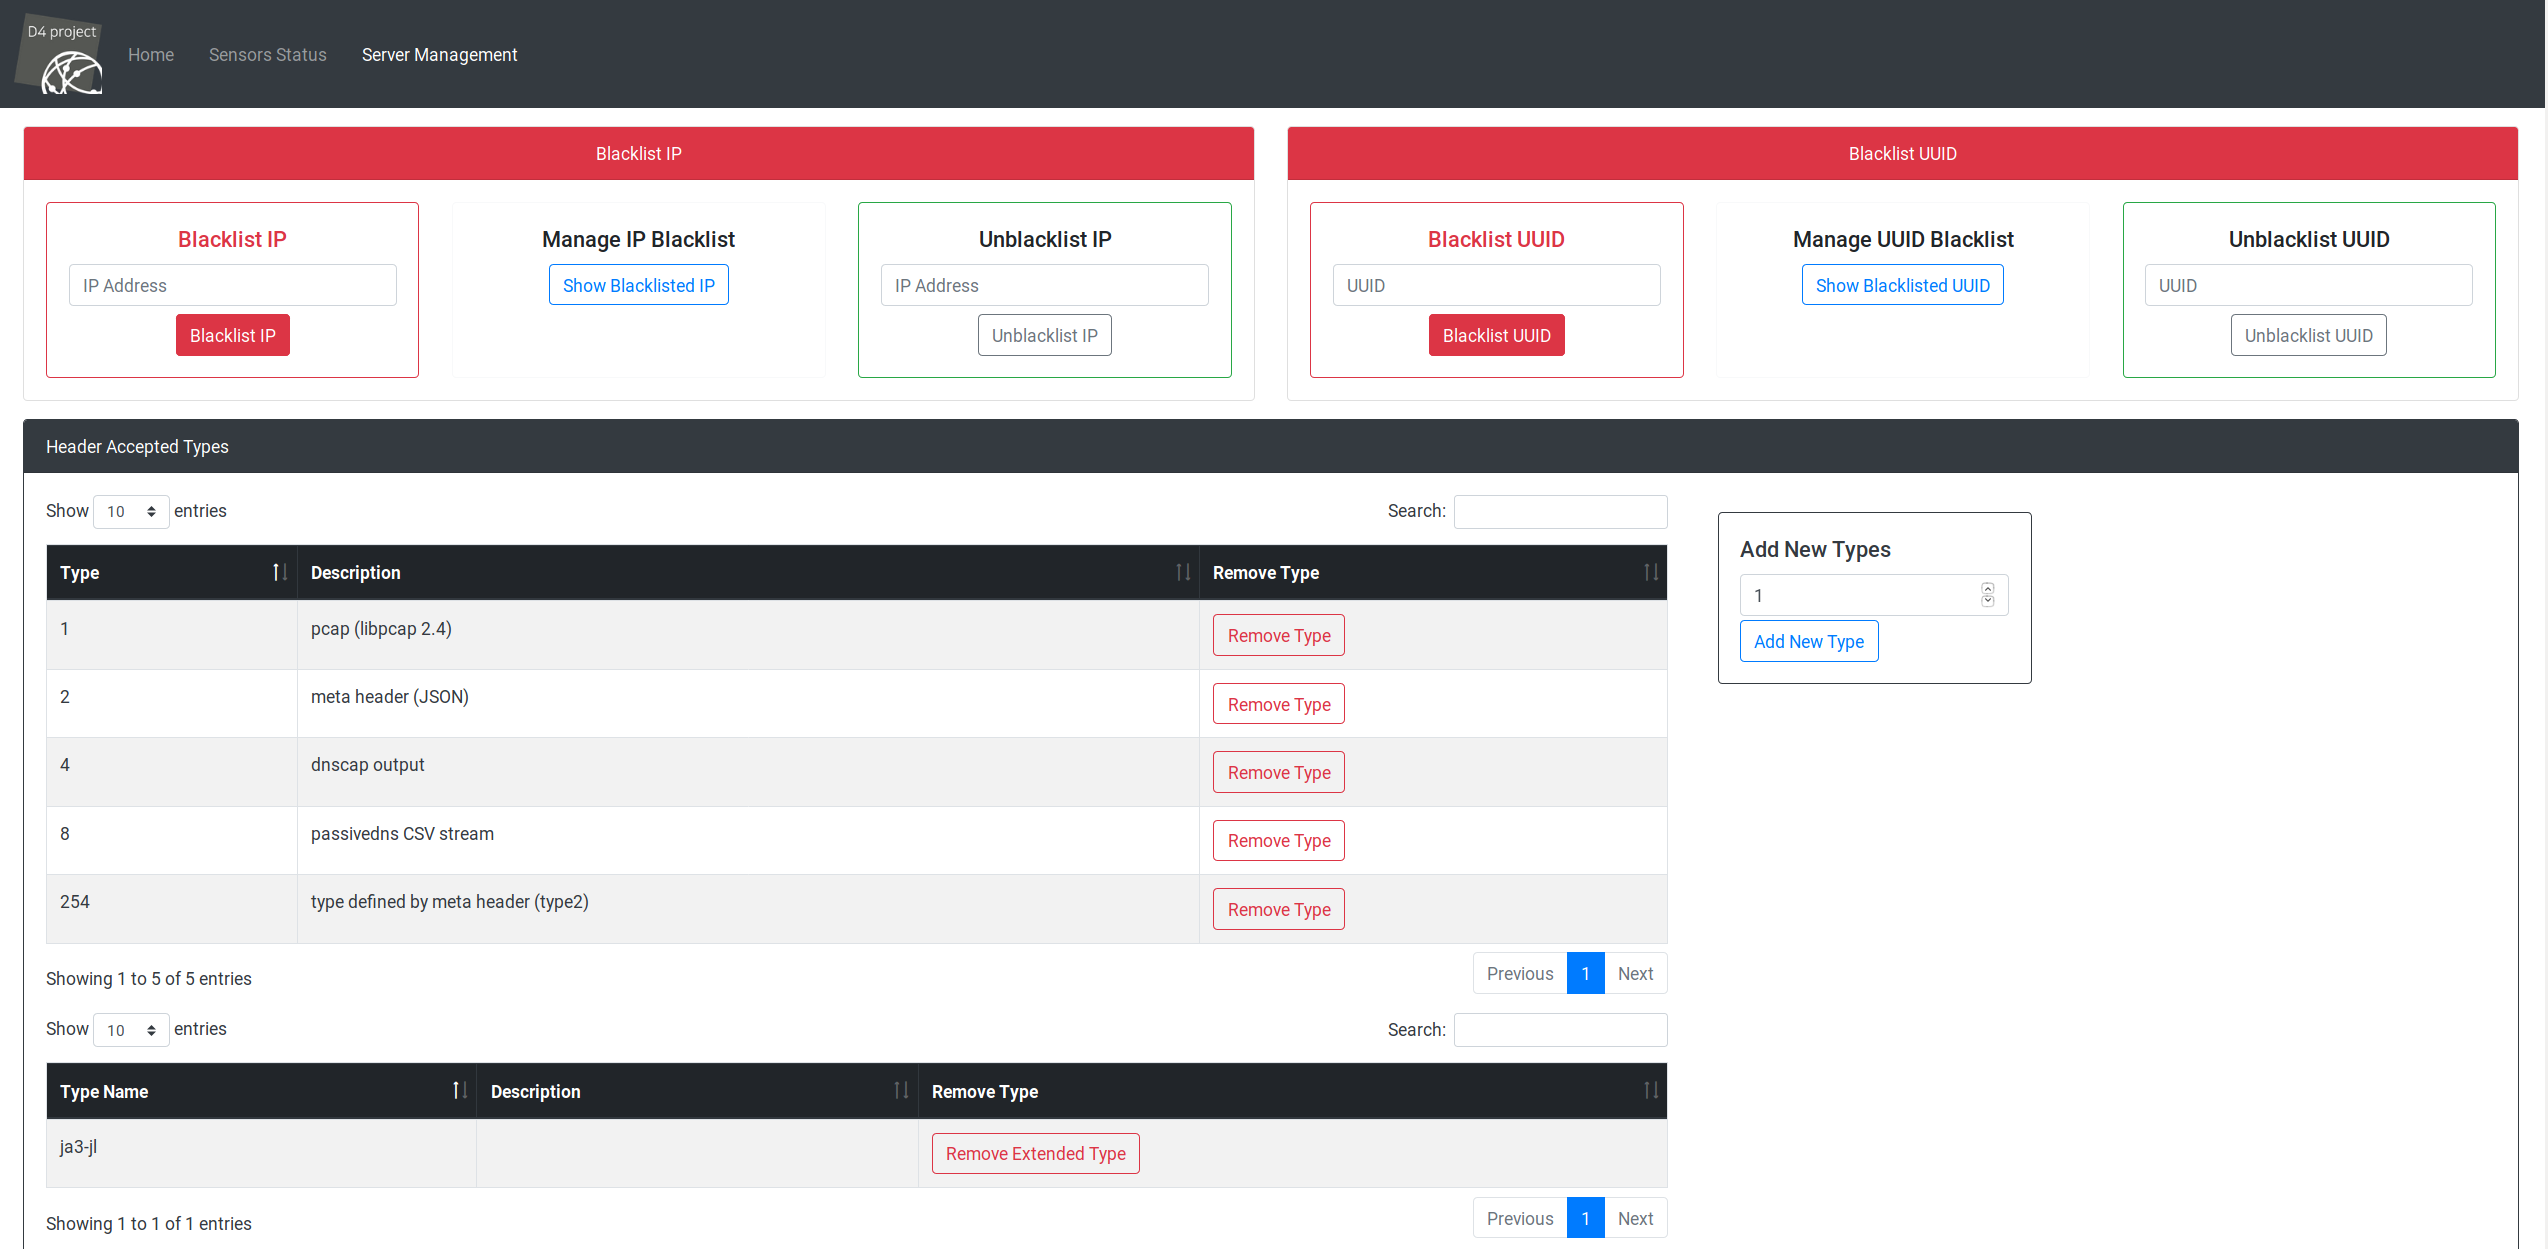
\includegraphics[width=\textwidth]{./d4-2.png}
\end{frame}

\begin{frame}
        \frametitle{D4 server - server management}
        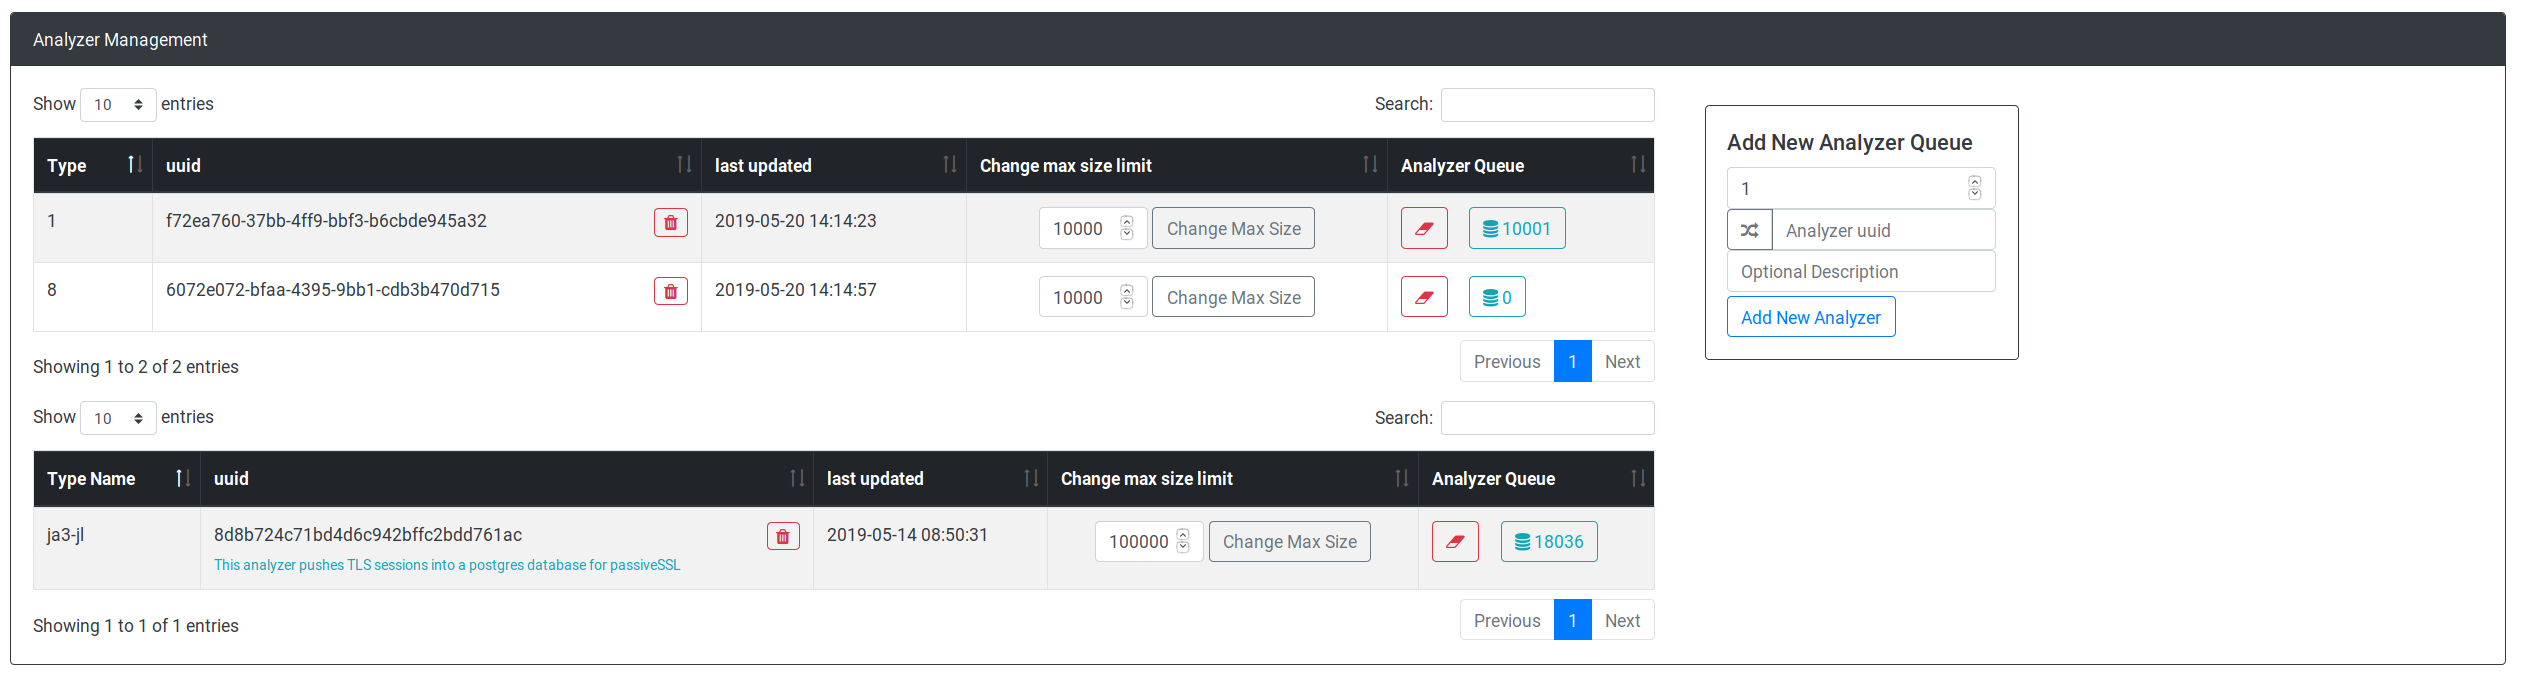
\includegraphics[width=\textwidth]{./d4-3.png}
\end{frame}

\begin{frame}
        \frametitle{D4 server - sensor overview}
        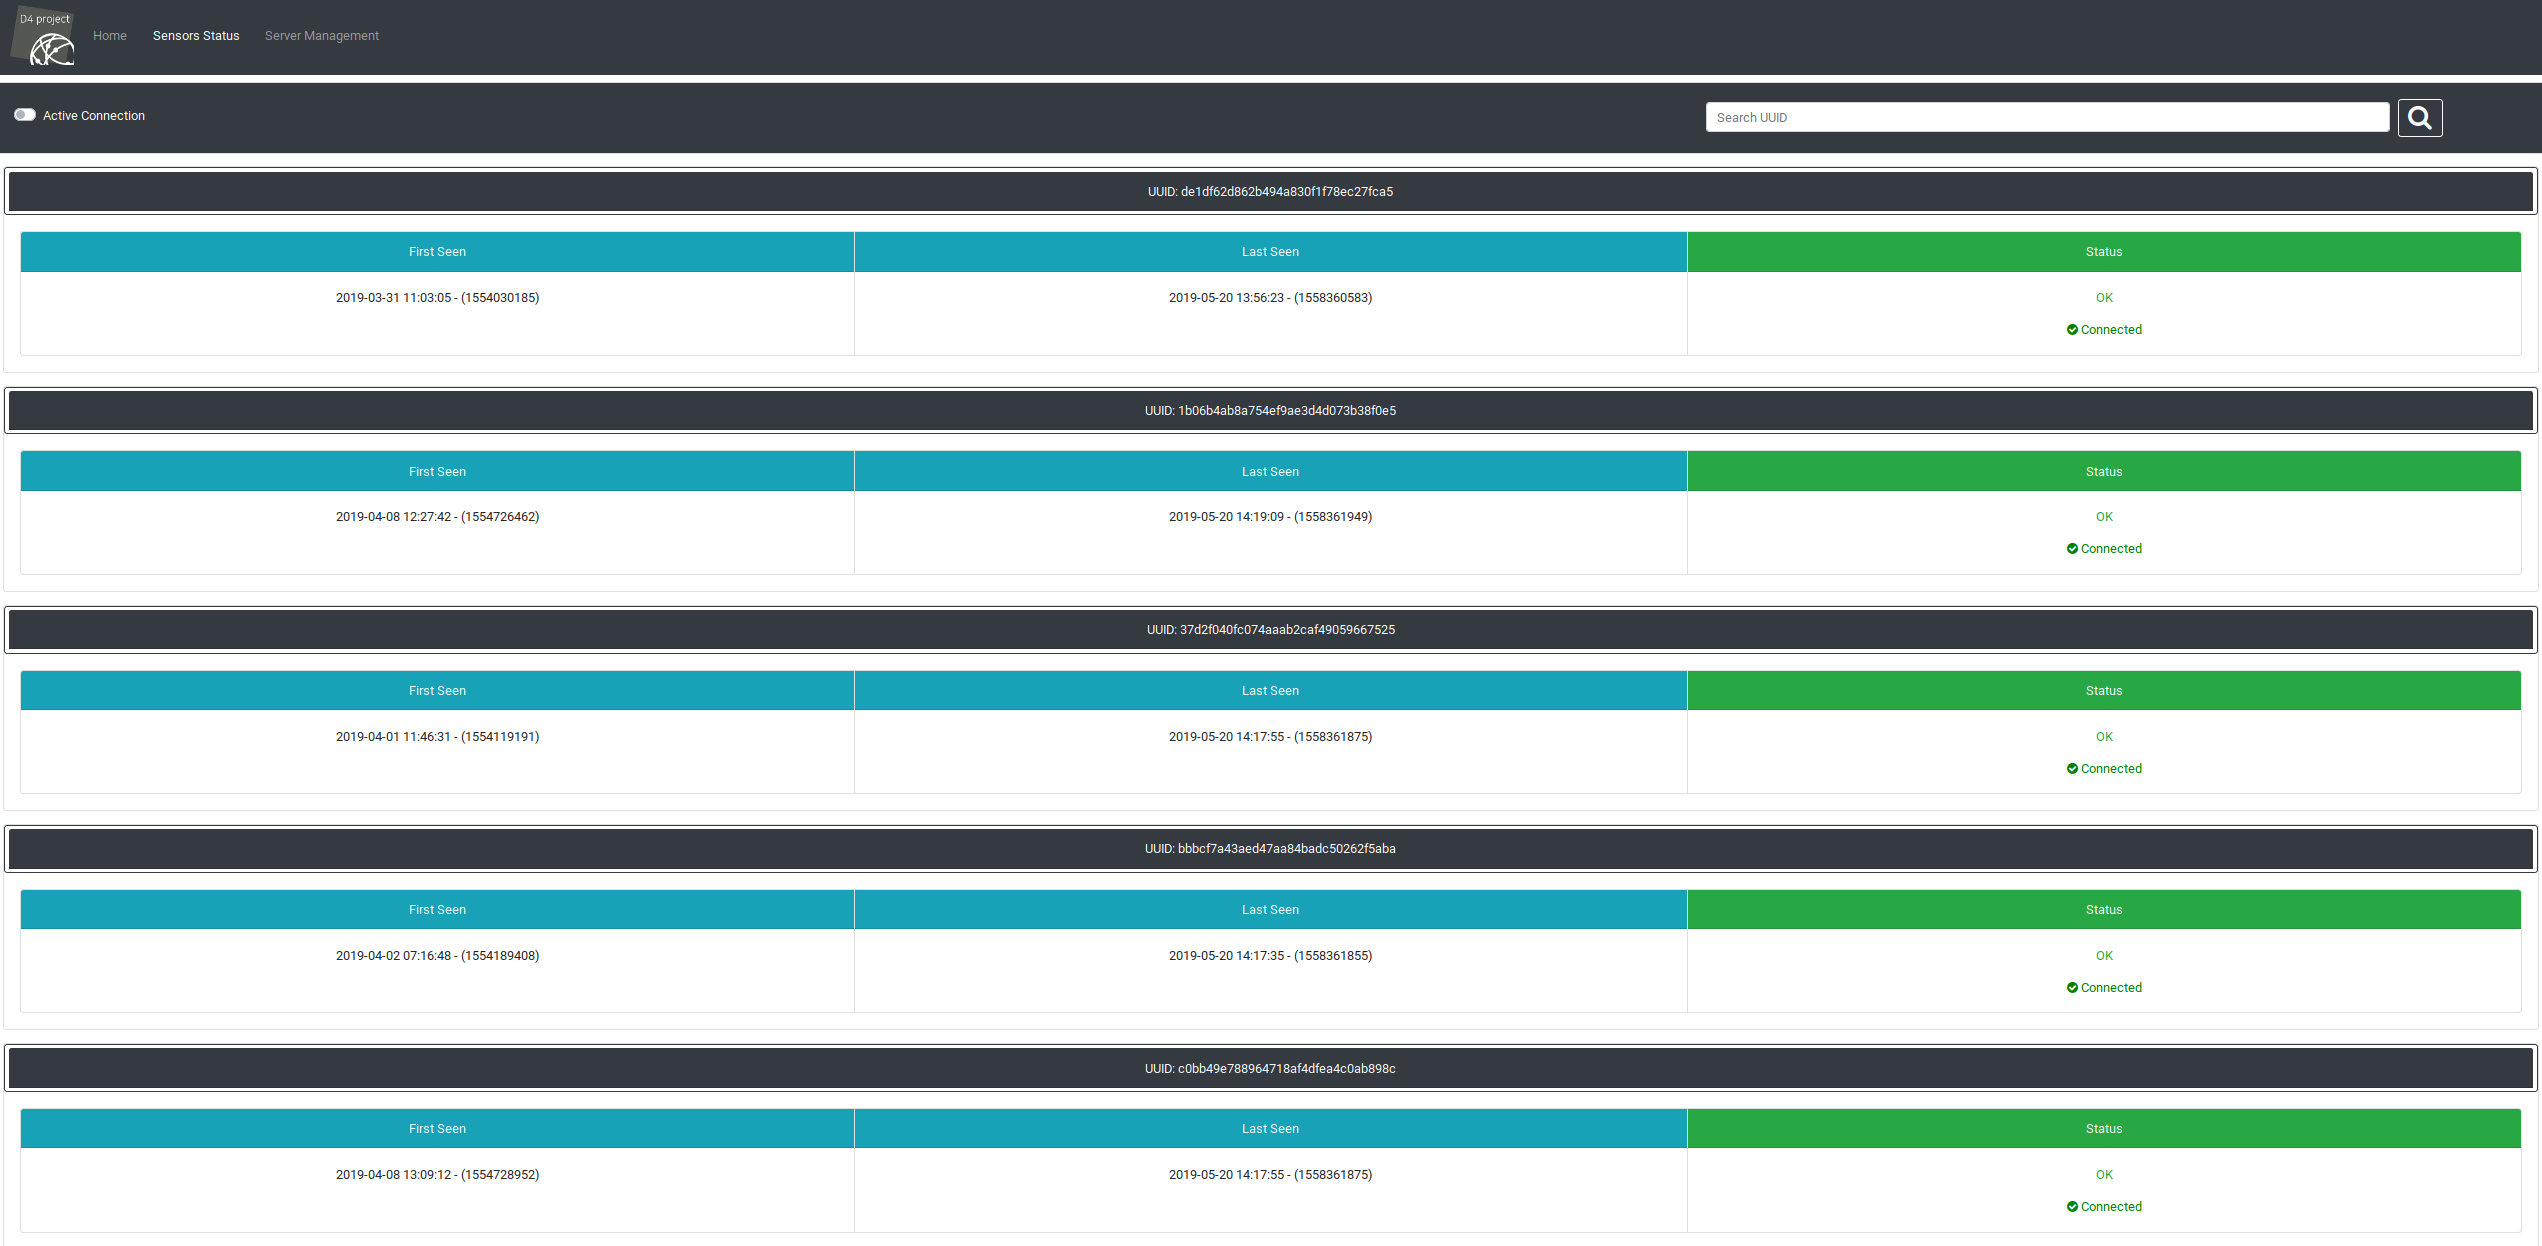
\includegraphics[width=\textwidth]{./d4-1.png}
\end{frame}


\begin{frame}
        \frametitle{D4 server - sensor management}
        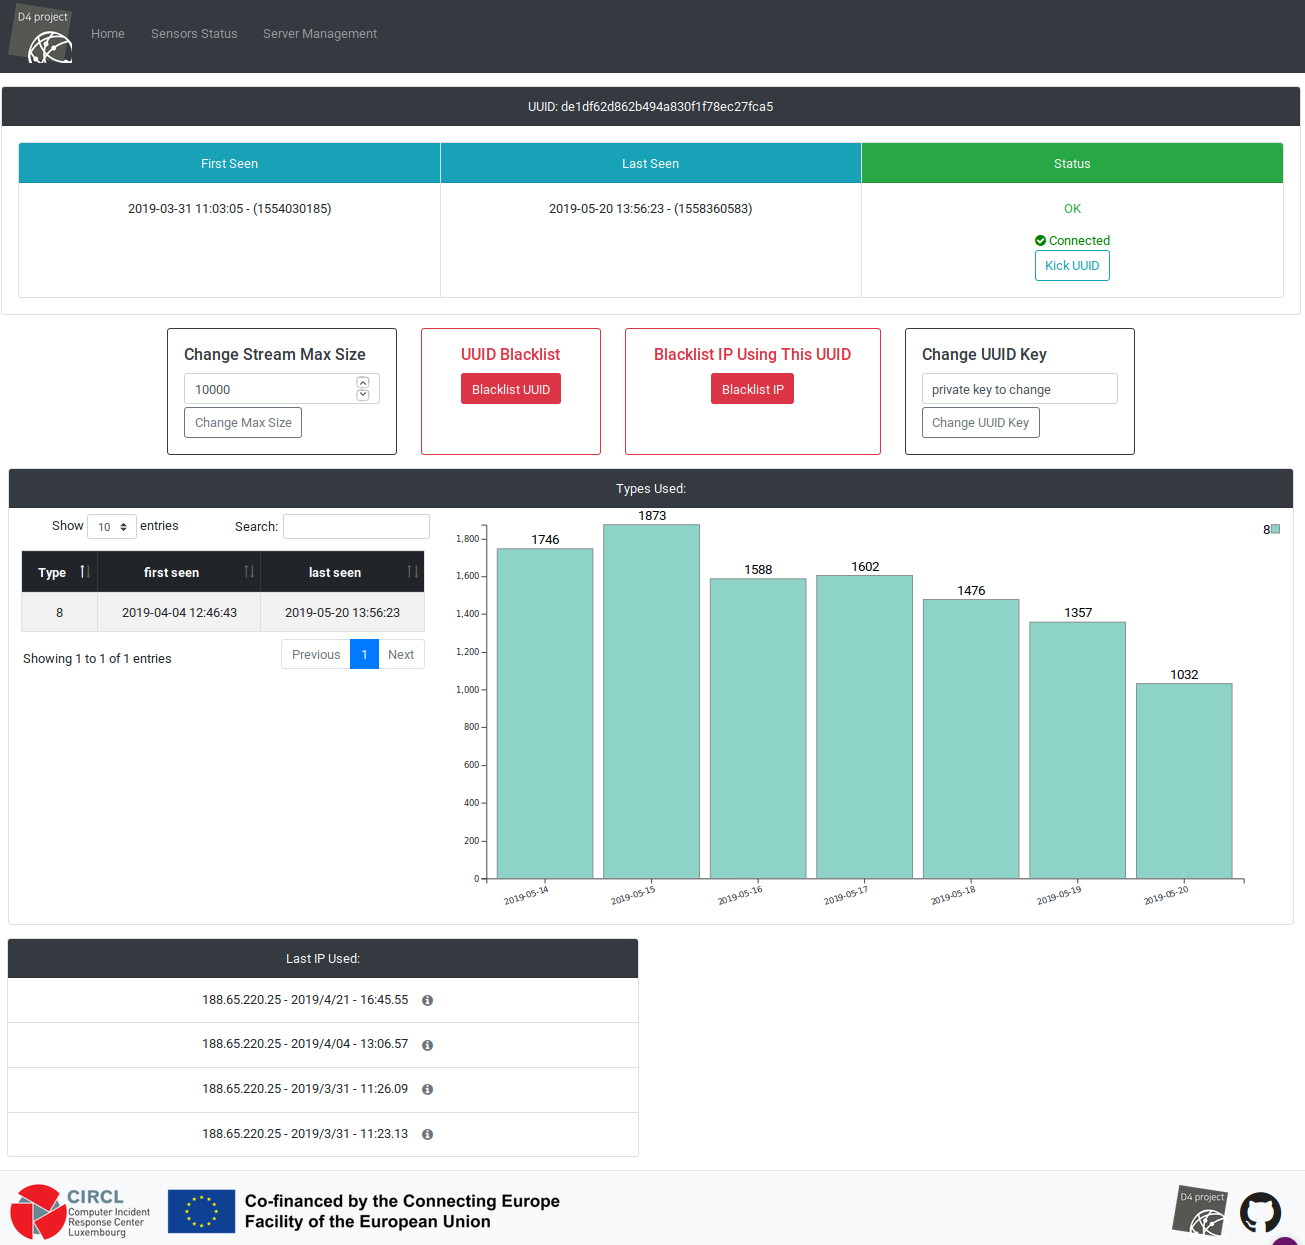
\includegraphics[width=\textwidth]{./d4-4.png}
\end{frame}

\begin{frame}
        \frametitle{}
        \begin{center}
         {\bf A distributed Network telescope to observe DDoS attacks}
        \end{center}
        \vspace{10pt}
        \begin{center}
          
\includegraphics[width=.7\textwidth]{eventhorizon.png}
        \end{center}
\end{frame}

\begin{frame}
        \frametitle{Motivation}
        DDoS Attacks produce an observable side-effect:
        \begin{center}
          \scalebox{0.8}{% GNUPLOT: LaTeX picture
\setlength{\unitlength}{0.240900pt}
\ifx\plotpoint\undefined\newsavebox{\plotpoint}\fi
\sbox{\plotpoint}{\rule[-0.200pt]{0.400pt}{0.400pt}}%
\begin{picture}(1500,900)(0,0)
\sbox{\plotpoint}{\rule[-0.200pt]{0.400pt}{0.400pt}}%
\put(231.0,190.0){\rule[-0.200pt]{291.007pt}{0.400pt}}
\put(231.0,190.0){\rule[-0.200pt]{4.818pt}{0.400pt}}
\put(211,190){\makebox(0,0)[r]{$0$}}
\put(1419.0,190.0){\rule[-0.200pt]{4.818pt}{0.400pt}}
\put(231.0,288.0){\rule[-0.200pt]{291.007pt}{0.400pt}}
\put(231.0,288.0){\rule[-0.200pt]{4.818pt}{0.400pt}}
\put(211,288){\makebox(0,0)[r]{$500000$}}
\put(1419.0,288.0){\rule[-0.200pt]{4.818pt}{0.400pt}}
\put(231.0,385.0){\rule[-0.200pt]{291.007pt}{0.400pt}}
\put(231.0,385.0){\rule[-0.200pt]{4.818pt}{0.400pt}}
\put(211,385){\makebox(0,0)[r]{$1\times10^{6}$}}
\put(1419.0,385.0){\rule[-0.200pt]{4.818pt}{0.400pt}}
\put(231.0,483.0){\rule[-0.200pt]{291.007pt}{0.400pt}}
\put(231.0,483.0){\rule[-0.200pt]{4.818pt}{0.400pt}}
\put(211,483){\makebox(0,0)[r]{$1.5\times10^{6}$}}
\put(1419.0,483.0){\rule[-0.200pt]{4.818pt}{0.400pt}}
\put(231.0,581.0){\rule[-0.200pt]{291.007pt}{0.400pt}}
\put(231.0,581.0){\rule[-0.200pt]{4.818pt}{0.400pt}}
\put(211,581){\makebox(0,0)[r]{$2\times10^{6}$}}
\put(1419.0,581.0){\rule[-0.200pt]{4.818pt}{0.400pt}}
\put(231.0,678.0){\rule[-0.200pt]{199.465pt}{0.400pt}}
\put(1419.0,678.0){\rule[-0.200pt]{4.818pt}{0.400pt}}
\put(231.0,678.0){\rule[-0.200pt]{4.818pt}{0.400pt}}
\put(211,678){\makebox(0,0)[r]{$2.5\times10^{6}$}}
\put(1419.0,678.0){\rule[-0.200pt]{4.818pt}{0.400pt}}
\put(231.0,776.0){\rule[-0.200pt]{291.007pt}{0.400pt}}
\put(231.0,776.0){\rule[-0.200pt]{4.818pt}{0.400pt}}
\put(211,776){\makebox(0,0)[r]{$3\times10^{6}$}}
\put(1419.0,776.0){\rule[-0.200pt]{4.818pt}{0.400pt}}
\put(262.0,190.0){\rule[-0.200pt]{0.400pt}{2.409pt}}
\put(372.0,190.0){\rule[-0.200pt]{0.400pt}{141.167pt}}
\put(372,170){\makebox(0,0)[l]{01/10}}
\put(372.0,190.0){\rule[-0.200pt]{0.400pt}{4.818pt}}
\put(482.0,190.0){\rule[-0.200pt]{0.400pt}{2.409pt}}
\put(592.0,190.0){\rule[-0.200pt]{0.400pt}{141.167pt}}
\put(592,170){\makebox(0,0)[l]{01/24}}
\put(592.0,190.0){\rule[-0.200pt]{0.400pt}{4.818pt}}
\put(702.0,190.0){\rule[-0.200pt]{0.400pt}{2.409pt}}
\put(811.0,190.0){\rule[-0.200pt]{0.400pt}{141.167pt}}
\put(811,170){\makebox(0,0)[l]{02/07}}
\put(811.0,190.0){\rule[-0.200pt]{0.400pt}{4.818pt}}
\put(921.0,190.0){\rule[-0.200pt]{0.400pt}{2.409pt}}
\put(1031.0,190.0){\rule[-0.200pt]{0.400pt}{141.167pt}}
\put(1031,170){\makebox(0,0)[l]{02/21}}
\put(1031.0,190.0){\rule[-0.200pt]{0.400pt}{4.818pt}}
\put(1141.0,190.0){\rule[-0.200pt]{0.400pt}{2.409pt}}
\put(1251.0,190.0){\rule[-0.200pt]{0.400pt}{116.596pt}}
\put(1251.0,756.0){\rule[-0.200pt]{0.400pt}{4.818pt}}
\put(1251,170){\makebox(0,0)[l]{03/07}}
\put(1251.0,190.0){\rule[-0.200pt]{0.400pt}{4.818pt}}
\put(1361.0,190.0){\rule[-0.200pt]{0.400pt}{2.409pt}}
\put(231.0,190.0){\rule[-0.200pt]{0.400pt}{141.167pt}}
\put(231.0,190.0){\rule[-0.200pt]{291.007pt}{0.400pt}}
\put(1439.0,190.0){\rule[-0.200pt]{0.400pt}{141.167pt}}
\put(231.0,776.0){\rule[-0.200pt]{291.007pt}{0.400pt}}
\put(261,747){\makebox(0,0)[l]{https://www.circl.lu/}}
\put(30,483){\makebox(0,0){Number of packets}}
\put(835,29){\makebox(0,0){date (month / day)}}
\put(835,838){\makebox(0,0){Backscatter traffic volume per 5 minutes in 2019}}
\put(1279,735){\makebox(0,0)[r]{backscatter}}
\put(1299.0,735.0){\rule[-0.200pt]{24.090pt}{0.400pt}}
\put(231,195){\usebox{\plotpoint}}
\put(231.0,195.0){\rule[-0.200pt]{0.400pt}{0.482pt}}
\put(231,194.67){\rule{0.241pt}{0.400pt}}
\multiput(231.00,194.17)(0.500,1.000){2}{\rule{0.120pt}{0.400pt}}
\put(231.0,195.0){\rule[-0.200pt]{0.400pt}{0.482pt}}
\put(232,196){\usebox{\plotpoint}}
\put(232.0,195.0){\usebox{\plotpoint}}
\put(232.0,195.0){\usebox{\plotpoint}}
\put(232.0,195.0){\usebox{\plotpoint}}
\put(232.0,195.0){\usebox{\plotpoint}}
\put(232.0,195.0){\usebox{\plotpoint}}
\put(232.0,195.0){\usebox{\plotpoint}}
\put(232.0,195.0){\usebox{\plotpoint}}
\put(232.0,195.0){\rule[-0.200pt]{0.400pt}{0.482pt}}
\put(232.0,195.0){\rule[-0.200pt]{0.400pt}{0.482pt}}
\put(232.0,195.0){\usebox{\plotpoint}}
\put(232.0,196.0){\usebox{\plotpoint}}
\put(233.0,196.0){\usebox{\plotpoint}}
\put(233.0,196.0){\usebox{\plotpoint}}
\put(233.0,196.0){\rule[-0.200pt]{0.400pt}{0.482pt}}
\put(233.0,196.0){\rule[-0.200pt]{0.400pt}{0.482pt}}
\put(233.0,196.0){\rule[-0.200pt]{0.400pt}{0.723pt}}
\put(233.0,198.0){\usebox{\plotpoint}}
\put(233,198.67){\rule{0.241pt}{0.400pt}}
\multiput(233.00,199.17)(0.500,-1.000){2}{\rule{0.120pt}{0.400pt}}
\put(233.0,198.0){\rule[-0.200pt]{0.400pt}{0.482pt}}
\put(234.0,199.0){\rule[-0.200pt]{0.400pt}{0.482pt}}
\put(234.0,199.0){\rule[-0.200pt]{0.400pt}{0.482pt}}
\put(234.0,199.0){\rule[-0.200pt]{0.400pt}{0.723pt}}
\put(234.0,201.0){\usebox{\plotpoint}}
\put(234.0,201.0){\rule[-0.200pt]{0.400pt}{0.482pt}}
\put(234.0,201.0){\rule[-0.200pt]{0.400pt}{0.482pt}}
\put(234,201.67){\rule{0.241pt}{0.400pt}}
\multiput(234.00,202.17)(0.500,-1.000){2}{\rule{0.120pt}{0.400pt}}
\put(234.0,201.0){\rule[-0.200pt]{0.400pt}{0.482pt}}
\put(235.0,202.0){\rule[-0.200pt]{0.400pt}{1.445pt}}
\put(235.0,204.0){\rule[-0.200pt]{0.400pt}{0.964pt}}
\put(235.0,204.0){\usebox{\plotpoint}}
\put(235.0,203.0){\rule[-0.200pt]{0.400pt}{0.482pt}}
\put(235.0,203.0){\usebox{\plotpoint}}
\put(235.0,203.0){\usebox{\plotpoint}}
\put(235,202.67){\rule{0.241pt}{0.400pt}}
\multiput(235.00,203.17)(0.500,-1.000){2}{\rule{0.120pt}{0.400pt}}
\put(235.0,203.0){\usebox{\plotpoint}}
\put(236,203){\usebox{\plotpoint}}
\put(236,203){\usebox{\plotpoint}}
\put(236.0,202.0){\usebox{\plotpoint}}
\put(236.0,202.0){\rule[-0.200pt]{0.400pt}{0.482pt}}
\put(236.0,203.0){\usebox{\plotpoint}}
\put(236.0,203.0){\rule[-0.200pt]{0.400pt}{0.482pt}}
\put(236,203.67){\rule{0.241pt}{0.400pt}}
\multiput(236.00,203.17)(0.500,1.000){2}{\rule{0.120pt}{0.400pt}}
\put(236.0,204.0){\usebox{\plotpoint}}
\put(237.0,204.0){\usebox{\plotpoint}}
\put(237.0,204.0){\usebox{\plotpoint}}
\put(237.0,203.0){\rule[-0.200pt]{0.400pt}{0.482pt}}
\put(237.0,203.0){\rule[-0.200pt]{0.400pt}{0.723pt}}
\put(237.0,204.0){\rule[-0.200pt]{0.400pt}{0.482pt}}
\put(237.0,204.0){\usebox{\plotpoint}}
\put(237.0,204.0){\usebox{\plotpoint}}
\put(237.0,204.0){\rule[-0.200pt]{0.400pt}{0.482pt}}
\put(237.0,205.0){\usebox{\plotpoint}}
\put(237.0,205.0){\usebox{\plotpoint}}
\put(237.0,204.0){\rule[-0.200pt]{0.400pt}{0.482pt}}
\put(237.0,204.0){\usebox{\plotpoint}}
\put(238.0,203.0){\usebox{\plotpoint}}
\put(238.0,203.0){\usebox{\plotpoint}}
\put(238.0,203.0){\usebox{\plotpoint}}
\put(238.0,203.0){\rule[-0.200pt]{0.400pt}{0.482pt}}
\put(238.0,202.0){\rule[-0.200pt]{0.400pt}{0.723pt}}
\put(238.0,202.0){\usebox{\plotpoint}}
\put(238.0,202.0){\usebox{\plotpoint}}
\put(238.0,202.0){\usebox{\plotpoint}}
\put(239.0,202.0){\usebox{\plotpoint}}
\put(239.0,201.0){\rule[-0.200pt]{0.400pt}{0.482pt}}
\put(239.0,201.0){\rule[-0.200pt]{0.400pt}{1.204pt}}
\put(239,204.67){\rule{0.241pt}{0.400pt}}
\multiput(239.00,204.17)(0.500,1.000){2}{\rule{0.120pt}{0.400pt}}
\put(239.0,205.0){\usebox{\plotpoint}}
\put(240.0,205.0){\usebox{\plotpoint}}
\put(240.0,205.0){\rule[-0.200pt]{0.400pt}{0.723pt}}
\put(240.0,201.0){\rule[-0.200pt]{0.400pt}{1.686pt}}
\put(240.0,201.0){\rule[-0.200pt]{0.400pt}{0.723pt}}
\put(240.0,202.0){\rule[-0.200pt]{0.400pt}{0.482pt}}
\put(240.0,202.0){\rule[-0.200pt]{0.400pt}{0.482pt}}
\put(240.0,202.0){\rule[-0.200pt]{0.400pt}{0.482pt}}
\put(240,202.67){\rule{0.241pt}{0.400pt}}
\multiput(240.00,202.17)(0.500,1.000){2}{\rule{0.120pt}{0.400pt}}
\put(240.0,202.0){\usebox{\plotpoint}}
\put(241.0,204.0){\usebox{\plotpoint}}
\put(241.0,202.0){\rule[-0.200pt]{0.400pt}{0.723pt}}
\put(241.0,202.0){\usebox{\plotpoint}}
\put(241.0,202.0){\usebox{\plotpoint}}
\put(241.0,202.0){\rule[-0.200pt]{0.400pt}{0.482pt}}
\put(241.0,203.0){\usebox{\plotpoint}}
\put(241.0,203.0){\usebox{\plotpoint}}
\put(241,202.67){\rule{0.241pt}{0.400pt}}
\multiput(241.00,202.17)(0.500,1.000){2}{\rule{0.120pt}{0.400pt}}
\put(241.0,203.0){\usebox{\plotpoint}}
\put(242,204){\usebox{\plotpoint}}
\put(242,204){\usebox{\plotpoint}}
\put(242,204){\usebox{\plotpoint}}
\put(242,204){\usebox{\plotpoint}}
\put(242,204){\usebox{\plotpoint}}
\put(242,204){\usebox{\plotpoint}}
\put(242,204){\usebox{\plotpoint}}
\put(242,204){\usebox{\plotpoint}}
\put(242,204){\usebox{\plotpoint}}
\put(242,204){\usebox{\plotpoint}}
\put(242.0,204.0){\usebox{\plotpoint}}
\put(242.0,203.0){\rule[-0.200pt]{0.400pt}{0.482pt}}
\put(242,203.67){\rule{0.241pt}{0.400pt}}
\multiput(242.00,204.17)(0.500,-1.000){2}{\rule{0.120pt}{0.400pt}}
\put(242.0,203.0){\rule[-0.200pt]{0.400pt}{0.482pt}}
\put(243,204){\usebox{\plotpoint}}
\put(243,204){\usebox{\plotpoint}}
\put(243,204){\usebox{\plotpoint}}
\put(243,204){\usebox{\plotpoint}}
\put(243,204){\usebox{\plotpoint}}
\put(243,204){\usebox{\plotpoint}}
\put(243,204){\usebox{\plotpoint}}
\put(243,204){\usebox{\plotpoint}}
\put(243,204){\usebox{\plotpoint}}
\put(243,204){\usebox{\plotpoint}}
\put(243,204){\usebox{\plotpoint}}
\put(243.0,203.0){\usebox{\plotpoint}}
\put(243.0,203.0){\usebox{\plotpoint}}
\put(244.0,201.0){\rule[-0.200pt]{0.400pt}{0.482pt}}
\put(244.0,201.0){\rule[-0.200pt]{0.400pt}{0.482pt}}
\put(243.67,197){\rule{0.400pt}{0.482pt}}
\multiput(243.17,197.00)(1.000,1.000){2}{\rule{0.400pt}{0.241pt}}
\put(244.0,197.0){\rule[-0.200pt]{0.400pt}{1.445pt}}
\put(245.0,195.0){\rule[-0.200pt]{0.400pt}{0.964pt}}
\put(245,194.67){\rule{0.241pt}{0.400pt}}
\multiput(245.00,195.17)(0.500,-1.000){2}{\rule{0.120pt}{0.400pt}}
\put(245.0,195.0){\usebox{\plotpoint}}
\put(246,195){\usebox{\plotpoint}}
\put(246,195){\usebox{\plotpoint}}
\put(246,195){\usebox{\plotpoint}}
\put(246,195){\usebox{\plotpoint}}
\put(246,195){\usebox{\plotpoint}}
\put(246,195){\usebox{\plotpoint}}
\put(246,195){\usebox{\plotpoint}}
\put(246,195){\usebox{\plotpoint}}
\put(246.0,195.0){\usebox{\plotpoint}}
\put(246.0,194.0){\rule[-0.200pt]{0.400pt}{0.482pt}}
\put(245.67,195){\rule{0.400pt}{0.482pt}}
\multiput(245.17,195.00)(1.000,1.000){2}{\rule{0.400pt}{0.241pt}}
\put(246.0,194.0){\usebox{\plotpoint}}
\put(247.0,195.0){\rule[-0.200pt]{0.400pt}{0.482pt}}
\put(247.0,195.0){\usebox{\plotpoint}}
\put(247.0,195.0){\usebox{\plotpoint}}
\put(247.0,195.0){\usebox{\plotpoint}}
\put(247.0,195.0){\usebox{\plotpoint}}
\put(247.0,195.0){\usebox{\plotpoint}}
\put(247.0,195.0){\usebox{\plotpoint}}
\put(247,195.67){\rule{0.241pt}{0.400pt}}
\multiput(247.00,196.17)(0.500,-1.000){2}{\rule{0.120pt}{0.400pt}}
\put(247.0,195.0){\rule[-0.200pt]{0.400pt}{0.482pt}}
\put(248,196){\usebox{\plotpoint}}
\put(248,196){\usebox{\plotpoint}}
\put(248,196){\usebox{\plotpoint}}
\put(248.0,196.0){\rule[-0.200pt]{0.400pt}{0.482pt}}
\put(248.0,196.0){\rule[-0.200pt]{0.400pt}{0.482pt}}
\put(248.0,196.0){\rule[-0.200pt]{0.400pt}{0.723pt}}
\put(248.0,196.0){\rule[-0.200pt]{0.400pt}{0.723pt}}
\put(248.0,196.0){\rule[-0.200pt]{0.400pt}{0.482pt}}
\put(248.0,197.0){\usebox{\plotpoint}}
\put(248.0,197.0){\usebox{\plotpoint}}
\put(249.0,197.0){\usebox{\plotpoint}}
\put(249.0,197.0){\usebox{\plotpoint}}
\put(249.0,197.0){\rule[-0.200pt]{0.400pt}{0.723pt}}
\put(249.0,199.0){\usebox{\plotpoint}}
\put(249.0,199.0){\rule[-0.200pt]{0.400pt}{0.723pt}}
\put(249,197.67){\rule{0.241pt}{0.400pt}}
\multiput(249.00,197.17)(0.500,1.000){2}{\rule{0.120pt}{0.400pt}}
\put(249.0,198.0){\rule[-0.200pt]{0.400pt}{0.964pt}}
\put(250,199){\usebox{\plotpoint}}
\put(250.0,199.0){\rule[-0.200pt]{0.400pt}{0.482pt}}
\put(250.0,200.0){\usebox{\plotpoint}}
\put(250.0,200.0){\usebox{\plotpoint}}
\put(250.0,199.0){\rule[-0.200pt]{0.400pt}{0.482pt}}
\put(250.0,199.0){\rule[-0.200pt]{0.400pt}{0.482pt}}
\put(250.0,199.0){\rule[-0.200pt]{0.400pt}{0.482pt}}
\put(250.0,199.0){\rule[-0.200pt]{0.400pt}{1.445pt}}
\put(250.0,201.0){\rule[-0.200pt]{0.400pt}{0.964pt}}
\put(250.0,201.0){\rule[-0.200pt]{0.400pt}{0.482pt}}
\put(250.0,202.0){\usebox{\plotpoint}}
\put(250.0,202.0){\rule[-0.200pt]{0.400pt}{0.482pt}}
\put(250.0,202.0){\rule[-0.200pt]{0.400pt}{0.482pt}}
\put(250.0,202.0){\usebox{\plotpoint}}
\put(251.0,201.0){\usebox{\plotpoint}}
\put(251.0,201.0){\usebox{\plotpoint}}
\put(251.0,200.0){\rule[-0.200pt]{0.400pt}{0.482pt}}
\put(251.0,200.0){\usebox{\plotpoint}}
\put(251.0,200.0){\usebox{\plotpoint}}
\put(251.0,200.0){\usebox{\plotpoint}}
\put(251.0,200.0){\usebox{\plotpoint}}
\put(251.0,200.0){\usebox{\plotpoint}}
\put(251.0,200.0){\usebox{\plotpoint}}
\put(251.0,200.0){\usebox{\plotpoint}}
\put(252.0,200.0){\rule[-0.200pt]{0.400pt}{0.723pt}}
\put(252.0,201.0){\rule[-0.200pt]{0.400pt}{0.482pt}}
\put(252.0,201.0){\rule[-0.200pt]{0.400pt}{0.964pt}}
\put(252.0,200.0){\rule[-0.200pt]{0.400pt}{1.204pt}}
\put(252.0,200.0){\rule[-0.200pt]{0.400pt}{0.482pt}}
\put(252.0,201.0){\usebox{\plotpoint}}
\put(252.0,201.0){\usebox{\plotpoint}}
\put(253.0,201.0){\usebox{\plotpoint}}
\put(253.0,201.0){\usebox{\plotpoint}}
\put(253.0,201.0){\usebox{\plotpoint}}
\put(253.0,201.0){\usebox{\plotpoint}}
\put(253.0,201.0){\usebox{\plotpoint}}
\put(253.0,201.0){\usebox{\plotpoint}}
\put(253.0,201.0){\usebox{\plotpoint}}
\put(254.0,201.0){\rule[-0.200pt]{0.400pt}{0.482pt}}
\put(254.0,201.0){\rule[-0.200pt]{0.400pt}{0.482pt}}
\put(254.0,201.0){\usebox{\plotpoint}}
\put(254,199.67){\rule{0.241pt}{0.400pt}}
\multiput(254.00,200.17)(0.500,-1.000){2}{\rule{0.120pt}{0.400pt}}
\put(254.0,201.0){\usebox{\plotpoint}}
\put(255.0,200.0){\rule[-0.200pt]{0.400pt}{0.723pt}}
\put(255.0,202.0){\usebox{\plotpoint}}
\put(255.0,202.0){\usebox{\plotpoint}}
\put(255.0,201.0){\rule[-0.200pt]{0.400pt}{0.482pt}}
\put(255.0,201.0){\usebox{\plotpoint}}
\put(255.0,201.0){\usebox{\plotpoint}}
\put(255.0,201.0){\usebox{\plotpoint}}
\put(255.0,201.0){\usebox{\plotpoint}}
\put(255.0,201.0){\rule[-0.200pt]{0.400pt}{0.964pt}}
\put(255.0,202.0){\rule[-0.200pt]{0.400pt}{0.723pt}}
\put(255.0,202.0){\usebox{\plotpoint}}
\put(256.0,200.0){\rule[-0.200pt]{0.400pt}{0.482pt}}
\put(256.0,200.0){\rule[-0.200pt]{0.400pt}{0.723pt}}
\put(256.0,200.0){\rule[-0.200pt]{0.400pt}{0.723pt}}
\put(256.0,200.0){\rule[-0.200pt]{0.400pt}{1.686pt}}
\put(256.0,202.0){\rule[-0.200pt]{0.400pt}{1.204pt}}
\put(256.0,202.0){\usebox{\plotpoint}}
\put(256.0,203.0){\usebox{\plotpoint}}
\put(257.0,203.0){\rule[-0.200pt]{0.400pt}{0.482pt}}
\put(257.0,202.0){\rule[-0.200pt]{0.400pt}{0.723pt}}
\put(257.0,202.0){\usebox{\plotpoint}}
\put(257.0,202.0){\usebox{\plotpoint}}
\put(257.0,202.0){\usebox{\plotpoint}}
\put(258.0,202.0){\rule[-0.200pt]{0.400pt}{0.482pt}}
\put(258.0,203.0){\usebox{\plotpoint}}
\put(258.0,203.0){\rule[-0.200pt]{0.400pt}{0.482pt}}
\put(258,202.67){\rule{0.241pt}{0.400pt}}
\multiput(258.00,203.17)(0.500,-1.000){2}{\rule{0.120pt}{0.400pt}}
\put(258.0,204.0){\usebox{\plotpoint}}
\put(259.0,203.0){\usebox{\plotpoint}}
\put(259.0,203.0){\usebox{\plotpoint}}
\put(259.0,203.0){\usebox{\plotpoint}}
\put(259.0,202.0){\rule[-0.200pt]{0.400pt}{0.482pt}}
\put(259.0,202.0){\usebox{\plotpoint}}
\put(259.0,201.0){\rule[-0.200pt]{0.400pt}{0.482pt}}
\put(258.67,200){\rule{0.400pt}{0.482pt}}
\multiput(258.17,201.00)(1.000,-1.000){2}{\rule{0.400pt}{0.241pt}}
\put(259.0,201.0){\usebox{\plotpoint}}
\put(260,200){\usebox{\plotpoint}}
\put(260.0,198.0){\rule[-0.200pt]{0.400pt}{0.482pt}}
\put(260.0,198.0){\usebox{\plotpoint}}
\put(260.0,195.0){\rule[-0.200pt]{0.400pt}{0.964pt}}
\put(260.0,195.0){\usebox{\plotpoint}}
\put(261.0,194.0){\usebox{\plotpoint}}
\put(261.0,194.0){\usebox{\plotpoint}}
\put(261.0,194.0){\usebox{\plotpoint}}
\put(261.0,194.0){\usebox{\plotpoint}}
\put(261.0,194.0){\usebox{\plotpoint}}
\put(261.0,194.0){\usebox{\plotpoint}}
\put(261.0,195.0){\usebox{\plotpoint}}
\put(262.0,194.0){\usebox{\plotpoint}}
\put(262.0,194.0){\usebox{\plotpoint}}
\put(262.0,193.0){\rule[-0.200pt]{0.400pt}{0.482pt}}
\put(262.0,193.0){\rule[-0.200pt]{0.400pt}{0.482pt}}
\put(262.0,194.0){\usebox{\plotpoint}}
\put(262.0,194.0){\usebox{\plotpoint}}
\put(263.0,194.0){\usebox{\plotpoint}}
\put(263.0,194.0){\usebox{\plotpoint}}
\put(263.0,194.0){\usebox{\plotpoint}}
\put(263.0,194.0){\usebox{\plotpoint}}
\put(263.0,194.0){\rule[-0.200pt]{0.400pt}{0.482pt}}
\put(263.0,194.0){\rule[-0.200pt]{0.400pt}{0.482pt}}
\put(263.0,194.0){\rule[-0.200pt]{0.400pt}{0.482pt}}
\put(263.0,195.0){\usebox{\plotpoint}}
\put(263.0,195.0){\usebox{\plotpoint}}
\put(264.0,195.0){\rule[-0.200pt]{0.400pt}{0.482pt}}
\put(264.0,196.0){\usebox{\plotpoint}}
\put(264.0,196.0){\usebox{\plotpoint}}
\put(264.0,195.0){\rule[-0.200pt]{0.400pt}{0.482pt}}
\put(264.0,195.0){\rule[-0.200pt]{0.400pt}{0.482pt}}
\put(264.0,196.0){\usebox{\plotpoint}}
\put(264.0,196.0){\usebox{\plotpoint}}
\put(264.0,196.0){\usebox{\plotpoint}}
\put(264.0,196.0){\rule[-0.200pt]{0.400pt}{0.482pt}}
\put(264.0,197.0){\usebox{\plotpoint}}
\put(264.0,197.0){\usebox{\plotpoint}}
\put(265.0,197.0){\rule[-0.200pt]{0.400pt}{0.482pt}}
\put(265.0,198.0){\usebox{\plotpoint}}
\put(265.0,198.0){\usebox{\plotpoint}}
\put(265.0,198.0){\usebox{\plotpoint}}
\put(265.0,198.0){\usebox{\plotpoint}}
\put(265.0,198.0){\usebox{\plotpoint}}
\put(265.0,198.0){\rule[-0.200pt]{0.400pt}{0.482pt}}
\put(265.0,199.0){\usebox{\plotpoint}}
\put(265.0,199.0){\rule[-0.200pt]{0.400pt}{0.723pt}}
\put(265.0,201.0){\usebox{\plotpoint}}
\put(265,200.67){\rule{0.241pt}{0.400pt}}
\multiput(265.00,201.17)(0.500,-1.000){2}{\rule{0.120pt}{0.400pt}}
\put(265.0,201.0){\usebox{\plotpoint}}
\put(266,201){\usebox{\plotpoint}}
\put(266.0,200.0){\usebox{\plotpoint}}
\put(266.0,200.0){\rule[-0.200pt]{0.400pt}{0.723pt}}
\put(266.0,200.0){\rule[-0.200pt]{0.400pt}{0.723pt}}
\put(266,200.67){\rule{0.241pt}{0.400pt}}
\multiput(266.00,200.17)(0.500,1.000){2}{\rule{0.120pt}{0.400pt}}
\put(266.0,200.0){\usebox{\plotpoint}}
\put(267.0,200.0){\rule[-0.200pt]{0.400pt}{0.482pt}}
\put(267.0,200.0){\rule[-0.200pt]{0.400pt}{0.723pt}}
\put(267.0,201.0){\rule[-0.200pt]{0.400pt}{0.482pt}}
\put(267.0,201.0){\rule[-0.200pt]{0.400pt}{1.204pt}}
\put(267.0,202.0){\rule[-0.200pt]{0.400pt}{0.964pt}}
\put(267.0,202.0){\usebox{\plotpoint}}
\put(267.0,202.0){\usebox{\plotpoint}}
\put(267.0,202.0){\usebox{\plotpoint}}
\put(267,200.67){\rule{0.241pt}{0.400pt}}
\multiput(267.00,201.17)(0.500,-1.000){2}{\rule{0.120pt}{0.400pt}}
\put(267.0,202.0){\usebox{\plotpoint}}
\put(268,201){\usebox{\plotpoint}}
\put(268,201){\usebox{\plotpoint}}
\put(268.0,201.0){\rule[-0.200pt]{0.400pt}{0.482pt}}
\put(268.0,200.0){\rule[-0.200pt]{0.400pt}{0.723pt}}
\put(268.0,200.0){\rule[-0.200pt]{0.400pt}{2.650pt}}
\put(268.0,202.0){\rule[-0.200pt]{0.400pt}{2.168pt}}
\put(268.0,202.0){\rule[-0.200pt]{0.400pt}{1.204pt}}
\put(268.0,201.0){\rule[-0.200pt]{0.400pt}{1.445pt}}
\put(268.0,201.0){\usebox{\plotpoint}}
\put(269.0,201.0){\usebox{\plotpoint}}
\put(269.0,201.0){\usebox{\plotpoint}}
\put(269.0,201.0){\usebox{\plotpoint}}
\put(269.0,201.0){\usebox{\plotpoint}}
\put(269.0,201.0){\usebox{\plotpoint}}
\put(269.0,201.0){\usebox{\plotpoint}}
\put(269.0,201.0){\usebox{\plotpoint}}
\put(269.0,201.0){\usebox{\plotpoint}}
\put(269.0,201.0){\usebox{\plotpoint}}
\put(269.0,201.0){\usebox{\plotpoint}}
\put(269.0,201.0){\usebox{\plotpoint}}
\put(270.0,200.0){\usebox{\plotpoint}}
\put(270.0,200.0){\rule[-0.200pt]{0.400pt}{0.482pt}}
\put(270.0,201.0){\usebox{\plotpoint}}
\put(270.0,201.0){\rule[-0.200pt]{0.400pt}{0.723pt}}
\put(270.0,201.0){\rule[-0.200pt]{0.400pt}{0.723pt}}
\put(270.0,201.0){\usebox{\plotpoint}}
\put(270.0,201.0){\usebox{\plotpoint}}
\put(270.0,201.0){\usebox{\plotpoint}}
\put(271.0,200.0){\usebox{\plotpoint}}
\put(271.0,200.0){\usebox{\plotpoint}}
\put(271.0,200.0){\usebox{\plotpoint}}
\put(271.0,200.0){\rule[-0.200pt]{0.400pt}{0.482pt}}
\put(271,199.67){\rule{0.241pt}{0.400pt}}
\multiput(271.00,199.17)(0.500,1.000){2}{\rule{0.120pt}{0.400pt}}
\put(271.0,200.0){\rule[-0.200pt]{0.400pt}{0.482pt}}
\put(272,201){\usebox{\plotpoint}}
\put(272.0,200.0){\usebox{\plotpoint}}
\put(272.0,200.0){\usebox{\plotpoint}}
\put(272.0,200.0){\usebox{\plotpoint}}
\put(272.0,200.0){\usebox{\plotpoint}}
\put(272.0,200.0){\usebox{\plotpoint}}
\put(272.0,200.0){\rule[-0.200pt]{0.400pt}{0.964pt}}
\put(272.0,202.0){\rule[-0.200pt]{0.400pt}{0.482pt}}
\put(272.0,202.0){\usebox{\plotpoint}}
\put(272.0,201.0){\rule[-0.200pt]{0.400pt}{0.482pt}}
\put(272.0,201.0){\usebox{\plotpoint}}
\put(273.0,201.0){\rule[-0.200pt]{0.400pt}{0.723pt}}
\put(273.0,203.0){\usebox{\plotpoint}}
\put(273.0,203.0){\usebox{\plotpoint}}
\put(273.0,203.0){\usebox{\plotpoint}}
\put(273.0,203.0){\rule[-0.200pt]{0.400pt}{0.723pt}}
\put(273.0,205.0){\usebox{\plotpoint}}
\put(273.0,205.0){\usebox{\plotpoint}}
\put(274.0,205.0){\usebox{\plotpoint}}
\put(274.0,205.0){\usebox{\plotpoint}}
\put(274.0,205.0){\usebox{\plotpoint}}
\put(274.0,205.0){\usebox{\plotpoint}}
\put(274,204.67){\rule{0.241pt}{0.400pt}}
\multiput(274.00,205.17)(0.500,-1.000){2}{\rule{0.120pt}{0.400pt}}
\put(274.0,205.0){\usebox{\plotpoint}}
\put(275,205){\usebox{\plotpoint}}
\put(275,205){\usebox{\plotpoint}}
\put(275,205){\usebox{\plotpoint}}
\put(275.0,203.0){\rule[-0.200pt]{0.400pt}{0.482pt}}
\put(275.0,203.0){\usebox{\plotpoint}}
\put(275.0,201.0){\rule[-0.200pt]{0.400pt}{0.723pt}}
\put(275.0,201.0){\rule[-0.200pt]{0.400pt}{0.964pt}}
\put(275.0,200.0){\rule[-0.200pt]{0.400pt}{1.204pt}}
\put(275.0,200.0){\usebox{\plotpoint}}
\put(276.0,197.0){\rule[-0.200pt]{0.400pt}{0.723pt}}
\put(276.0,197.0){\usebox{\plotpoint}}
\put(277.0,196.0){\usebox{\plotpoint}}
\put(277.0,196.0){\usebox{\plotpoint}}
\put(277.0,196.0){\usebox{\plotpoint}}
\put(277.0,196.0){\usebox{\plotpoint}}
\put(277.0,195.0){\rule[-0.200pt]{0.400pt}{0.482pt}}
\put(277.0,195.0){\usebox{\plotpoint}}
\put(277.0,196.0){\usebox{\plotpoint}}
\put(278.0,196.0){\rule[-0.200pt]{0.400pt}{0.482pt}}
\put(278.0,196.0){\rule[-0.200pt]{0.400pt}{0.482pt}}
\put(278.0,196.0){\rule[-0.200pt]{0.400pt}{0.482pt}}
\put(278.0,196.0){\rule[-0.200pt]{0.400pt}{0.482pt}}
\put(278.0,196.0){\usebox{\plotpoint}}
\put(278,195.67){\rule{0.241pt}{0.400pt}}
\multiput(278.00,195.17)(0.500,1.000){2}{\rule{0.120pt}{0.400pt}}
\put(278.0,196.0){\usebox{\plotpoint}}
\put(279.0,196.0){\usebox{\plotpoint}}
\put(279.0,196.0){\rule[-0.200pt]{0.400pt}{1.204pt}}
\put(279.0,197.0){\rule[-0.200pt]{0.400pt}{0.964pt}}
\put(279.0,197.0){\usebox{\plotpoint}}
\put(279.0,197.0){\usebox{\plotpoint}}
\put(279.0,197.0){\rule[-0.200pt]{0.400pt}{0.482pt}}
\put(279.0,197.0){\rule[-0.200pt]{0.400pt}{0.482pt}}
\put(279.0,197.0){\rule[-0.200pt]{0.400pt}{0.482pt}}
\put(279.0,198.0){\usebox{\plotpoint}}
\put(279.0,198.0){\usebox{\plotpoint}}
\put(280.0,198.0){\rule[-0.200pt]{0.400pt}{0.482pt}}
\put(280.0,198.0){\rule[-0.200pt]{0.400pt}{0.482pt}}
\put(280.0,198.0){\rule[-0.200pt]{0.400pt}{0.482pt}}
\put(280.0,199.0){\usebox{\plotpoint}}
\put(280.0,199.0){\usebox{\plotpoint}}
\put(280.0,198.0){\rule[-0.200pt]{0.400pt}{0.482pt}}
\put(280.0,198.0){\rule[-0.200pt]{0.400pt}{0.723pt}}
\put(280,198.67){\rule{0.241pt}{0.400pt}}
\multiput(280.00,198.17)(0.500,1.000){2}{\rule{0.120pt}{0.400pt}}
\put(280.0,199.0){\rule[-0.200pt]{0.400pt}{0.482pt}}
\put(281.0,200.0){\rule[-0.200pt]{0.400pt}{0.723pt}}
\put(281.0,201.0){\rule[-0.200pt]{0.400pt}{0.482pt}}
\put(281.0,201.0){\usebox{\plotpoint}}
\put(281.0,199.0){\rule[-0.200pt]{0.400pt}{0.723pt}}
\put(281.0,199.0){\usebox{\plotpoint}}
\put(281.0,199.0){\usebox{\plotpoint}}
\put(281.0,199.0){\rule[-0.200pt]{0.400pt}{0.482pt}}
\put(281.0,199.0){\rule[-0.200pt]{0.400pt}{0.482pt}}
\put(281.0,199.0){\rule[-0.200pt]{0.400pt}{0.482pt}}
\put(281.0,200.0){\usebox{\plotpoint}}
\put(281.0,200.0){\usebox{\plotpoint}}
\put(281,199.67){\rule{0.241pt}{0.400pt}}
\multiput(281.00,199.17)(0.500,1.000){2}{\rule{0.120pt}{0.400pt}}
\put(281.0,200.0){\usebox{\plotpoint}}
\put(282,201){\usebox{\plotpoint}}
\put(282.0,201.0){\rule[-0.200pt]{0.400pt}{0.723pt}}
\put(282.0,202.0){\rule[-0.200pt]{0.400pt}{0.482pt}}
\put(282.0,202.0){\rule[-0.200pt]{0.400pt}{0.482pt}}
\put(282.0,201.0){\rule[-0.200pt]{0.400pt}{0.723pt}}
\put(282.0,201.0){\rule[-0.200pt]{0.400pt}{0.964pt}}
\put(282.0,202.0){\rule[-0.200pt]{0.400pt}{0.723pt}}
\put(282.0,202.0){\usebox{\plotpoint}}
\put(283.0,202.0){\usebox{\plotpoint}}
\put(283.0,201.0){\rule[-0.200pt]{0.400pt}{0.482pt}}
\put(283.0,201.0){\usebox{\plotpoint}}
\put(283.0,200.0){\rule[-0.200pt]{0.400pt}{0.482pt}}
\put(283.0,200.0){\rule[-0.200pt]{0.400pt}{0.964pt}}
\put(283.0,202.0){\rule[-0.200pt]{0.400pt}{0.482pt}}
\put(283.0,202.0){\usebox{\plotpoint}}
\put(283.0,201.0){\rule[-0.200pt]{0.400pt}{0.482pt}}
\put(283.0,201.0){\usebox{\plotpoint}}
\put(283,199.67){\rule{0.241pt}{0.400pt}}
\multiput(283.00,200.17)(0.500,-1.000){2}{\rule{0.120pt}{0.400pt}}
\put(283.0,201.0){\usebox{\plotpoint}}
\put(284,200){\usebox{\plotpoint}}
\put(284.0,200.0){\rule[-0.200pt]{0.400pt}{0.723pt}}
\put(284.0,200.0){\rule[-0.200pt]{0.400pt}{0.723pt}}
\put(284.0,200.0){\rule[-0.200pt]{0.400pt}{0.964pt}}
\put(284.0,200.0){\rule[-0.200pt]{0.400pt}{0.964pt}}
\put(284.0,200.0){\rule[-0.200pt]{0.400pt}{0.482pt}}
\put(284.0,200.0){\rule[-0.200pt]{0.400pt}{0.482pt}}
\put(284,204.67){\rule{0.241pt}{0.400pt}}
\multiput(284.00,204.17)(0.500,1.000){2}{\rule{0.120pt}{0.400pt}}
\put(284.0,200.0){\rule[-0.200pt]{0.400pt}{1.204pt}}
\put(285.0,202.0){\rule[-0.200pt]{0.400pt}{0.964pt}}
\put(285.0,202.0){\rule[-0.200pt]{0.400pt}{0.482pt}}
\put(285.0,201.0){\rule[-0.200pt]{0.400pt}{0.723pt}}
\put(285.0,201.0){\usebox{\plotpoint}}
\put(285.0,201.0){\usebox{\plotpoint}}
\put(285.0,201.0){\rule[-0.200pt]{0.400pt}{0.482pt}}
\put(285,200.67){\rule{0.241pt}{0.400pt}}
\multiput(285.00,200.17)(0.500,1.000){2}{\rule{0.120pt}{0.400pt}}
\put(285.0,201.0){\rule[-0.200pt]{0.400pt}{0.482pt}}
\put(286,202){\usebox{\plotpoint}}
\put(286.0,199.0){\rule[-0.200pt]{0.400pt}{0.723pt}}
\put(286.0,199.0){\rule[-0.200pt]{0.400pt}{0.482pt}}
\put(286.0,200.0){\usebox{\plotpoint}}
\put(286.0,200.0){\rule[-0.200pt]{0.400pt}{0.964pt}}
\put(286.0,200.0){\rule[-0.200pt]{0.400pt}{0.964pt}}
\put(286.0,200.0){\usebox{\plotpoint}}
\put(287.0,200.0){\rule[-0.200pt]{0.400pt}{0.723pt}}
\put(287.0,200.0){\rule[-0.200pt]{0.400pt}{0.723pt}}
\put(287.0,200.0){\rule[-0.200pt]{0.400pt}{1.927pt}}
\put(287.0,200.0){\rule[-0.200pt]{0.400pt}{1.927pt}}
\put(287.0,200.0){\rule[-0.200pt]{0.400pt}{0.482pt}}
\put(287.0,200.0){\rule[-0.200pt]{0.400pt}{0.482pt}}
\put(287.0,200.0){\usebox{\plotpoint}}
\put(288.0,200.0){\rule[-0.200pt]{0.400pt}{1.445pt}}
\put(288.0,201.0){\rule[-0.200pt]{0.400pt}{1.204pt}}
\put(288.0,201.0){\usebox{\plotpoint}}
\put(288.0,201.0){\usebox{\plotpoint}}
\put(288.0,201.0){\rule[-0.200pt]{0.400pt}{0.482pt}}
\put(288.0,201.0){\rule[-0.200pt]{0.400pt}{0.482pt}}
\put(288.0,201.0){\rule[-0.200pt]{0.400pt}{0.723pt}}
\put(288.0,203.0){\usebox{\plotpoint}}
\put(288.0,203.0){\usebox{\plotpoint}}
\put(289.0,203.0){\usebox{\plotpoint}}
\put(289.0,203.0){\usebox{\plotpoint}}
\put(289.0,203.0){\usebox{\plotpoint}}
\put(290.0,203.0){\usebox{\plotpoint}}
\put(290.0,202.0){\rule[-0.200pt]{0.400pt}{0.482pt}}
\put(290.0,202.0){\usebox{\plotpoint}}
\put(291.0,201.0){\usebox{\plotpoint}}
\put(291.0,201.0){\rule[-0.200pt]{0.400pt}{0.482pt}}
\put(291.0,197.0){\rule[-0.200pt]{0.400pt}{1.445pt}}
\put(291.0,197.0){\usebox{\plotpoint}}
\put(292.0,195.0){\rule[-0.200pt]{0.400pt}{0.482pt}}
\put(292.0,195.0){\usebox{\plotpoint}}
\put(292.0,195.0){\usebox{\plotpoint}}
\put(292.0,195.0){\usebox{\plotpoint}}
\put(293.0,194.0){\usebox{\plotpoint}}
\put(293.0,194.0){\rule[-0.200pt]{0.400pt}{0.964pt}}
\put(293.0,194.0){\rule[-0.200pt]{0.400pt}{0.964pt}}
\put(293.0,194.0){\rule[-0.200pt]{0.400pt}{0.723pt}}
\put(293.0,197.0){\usebox{\plotpoint}}
\put(294.0,197.0){\rule[-0.200pt]{0.400pt}{0.964pt}}
\put(294.0,194.0){\rule[-0.200pt]{0.400pt}{1.686pt}}
\put(294.0,194.0){\usebox{\plotpoint}}
\put(294.0,194.0){\usebox{\plotpoint}}
\put(294.0,194.0){\rule[-0.200pt]{0.400pt}{0.482pt}}
\put(294,193.67){\rule{0.241pt}{0.400pt}}
\multiput(294.00,194.17)(0.500,-1.000){2}{\rule{0.120pt}{0.400pt}}
\put(294.0,195.0){\usebox{\plotpoint}}
\put(295,194){\usebox{\plotpoint}}
\put(295.0,194.0){\rule[-0.200pt]{0.400pt}{0.723pt}}
\put(295.0,194.0){\rule[-0.200pt]{0.400pt}{0.723pt}}
\put(295.0,194.0){\rule[-0.200pt]{0.400pt}{0.723pt}}
\put(295.0,195.0){\rule[-0.200pt]{0.400pt}{0.482pt}}
\put(295.0,195.0){\usebox{\plotpoint}}
\put(295.0,196.0){\usebox{\plotpoint}}
\put(296.0,196.0){\usebox{\plotpoint}}
\put(296.0,196.0){\usebox{\plotpoint}}
\put(296.0,196.0){\usebox{\plotpoint}}
\put(296.0,196.0){\usebox{\plotpoint}}
\put(296.0,196.0){\rule[-0.200pt]{0.400pt}{0.723pt}}
\put(296.0,198.0){\usebox{\plotpoint}}
\put(296.0,198.0){\usebox{\plotpoint}}
\put(296.0,199.0){\usebox{\plotpoint}}
\put(297.0,198.0){\usebox{\plotpoint}}
\put(297.0,198.0){\rule[-0.200pt]{0.400pt}{0.964pt}}
\put(297.0,201.0){\usebox{\plotpoint}}
\put(297,201.67){\rule{0.241pt}{0.400pt}}
\multiput(297.00,202.17)(0.500,-1.000){2}{\rule{0.120pt}{0.400pt}}
\put(297.0,201.0){\rule[-0.200pt]{0.400pt}{0.482pt}}
\put(298,202){\usebox{\plotpoint}}
\put(298,202){\usebox{\plotpoint}}
\put(298,202){\usebox{\plotpoint}}
\put(298,202){\usebox{\plotpoint}}
\put(298.0,202.0){\rule[-0.200pt]{0.400pt}{0.482pt}}
\put(298.0,202.0){\rule[-0.200pt]{0.400pt}{0.482pt}}
\put(298.0,202.0){\usebox{\plotpoint}}
\put(298.0,202.0){\usebox{\plotpoint}}
\put(298.0,202.0){\rule[-0.200pt]{0.400pt}{0.964pt}}
\put(298.0,203.0){\rule[-0.200pt]{0.400pt}{0.723pt}}
\put(298.0,203.0){\usebox{\plotpoint}}
\put(298.0,203.0){\usebox{\plotpoint}}
\put(298.0,203.0){\usebox{\plotpoint}}
\put(299.0,203.0){\usebox{\plotpoint}}
\put(299.0,203.0){\usebox{\plotpoint}}
\put(299.0,203.0){\rule[-0.200pt]{0.400pt}{0.723pt}}
\put(299.0,204.0){\rule[-0.200pt]{0.400pt}{0.482pt}}
\put(299.0,204.0){\rule[-0.200pt]{0.400pt}{0.482pt}}
\put(299.0,203.0){\rule[-0.200pt]{0.400pt}{0.723pt}}
\put(299.0,203.0){\rule[-0.200pt]{0.400pt}{0.723pt}}
\put(298.67,204){\rule{0.400pt}{0.482pt}}
\multiput(298.17,204.00)(1.000,1.000){2}{\rule{0.400pt}{0.241pt}}
\put(299.0,204.0){\rule[-0.200pt]{0.400pt}{0.482pt}}
\put(300.0,202.0){\rule[-0.200pt]{0.400pt}{0.964pt}}
\put(300.0,202.0){\rule[-0.200pt]{0.400pt}{0.723pt}}
\put(300.0,202.0){\rule[-0.200pt]{0.400pt}{0.723pt}}
\put(300.0,202.0){\rule[-0.200pt]{0.400pt}{0.723pt}}
\put(300.0,202.0){\rule[-0.200pt]{0.400pt}{0.723pt}}
\put(300.0,202.0){\usebox{\plotpoint}}
\put(300.0,202.0){\usebox{\plotpoint}}
\put(300,201.67){\rule{0.241pt}{0.400pt}}
\multiput(300.00,202.17)(0.500,-1.000){2}{\rule{0.120pt}{0.400pt}}
\put(300.0,202.0){\usebox{\plotpoint}}
\put(301.0,202.0){\usebox{\plotpoint}}
\put(301.0,202.0){\usebox{\plotpoint}}
\put(301.0,202.0){\usebox{\plotpoint}}
\put(301.0,202.0){\usebox{\plotpoint}}
\put(301.0,202.0){\rule[-0.200pt]{0.400pt}{0.482pt}}
\put(301.0,202.0){\rule[-0.200pt]{0.400pt}{0.482pt}}
\put(301.0,202.0){\usebox{\plotpoint}}
\put(302.0,202.0){\usebox{\plotpoint}}
\put(302.0,202.0){\usebox{\plotpoint}}
\put(302.0,202.0){\rule[-0.200pt]{0.400pt}{1.204pt}}
\put(302.0,202.0){\rule[-0.200pt]{0.400pt}{1.204pt}}
\put(302.0,202.0){\rule[-0.200pt]{0.400pt}{0.482pt}}
\put(302.0,202.0){\rule[-0.200pt]{0.400pt}{0.482pt}}
\put(302.0,202.0){\usebox{\plotpoint}}
\put(303.0,202.0){\usebox{\plotpoint}}
\put(303.0,202.0){\usebox{\plotpoint}}
\put(303.0,202.0){\usebox{\plotpoint}}
\put(303.0,202.0){\usebox{\plotpoint}}
\put(303.0,202.0){\rule[-0.200pt]{0.400pt}{0.964pt}}
\put(303.0,203.0){\rule[-0.200pt]{0.400pt}{0.723pt}}
\put(303.0,203.0){\rule[-0.200pt]{0.400pt}{0.482pt}}
\put(302.67,202){\rule{0.400pt}{0.482pt}}
\multiput(302.17,203.00)(1.000,-1.000){2}{\rule{0.400pt}{0.241pt}}
\put(303.0,204.0){\usebox{\plotpoint}}
\put(304,202){\usebox{\plotpoint}}
\put(304,202){\usebox{\plotpoint}}
\put(304,202){\usebox{\plotpoint}}
\put(304,202){\usebox{\plotpoint}}
\put(304.0,201.0){\usebox{\plotpoint}}
\put(304.0,201.0){\rule[-0.200pt]{0.400pt}{0.482pt}}
\put(304.0,201.0){\rule[-0.200pt]{0.400pt}{0.482pt}}
\put(304,201.67){\rule{0.241pt}{0.400pt}}
\multiput(304.00,201.17)(0.500,1.000){2}{\rule{0.120pt}{0.400pt}}
\put(304.0,201.0){\usebox{\plotpoint}}
\put(305,203){\usebox{\plotpoint}}
\put(305.0,202.0){\usebox{\plotpoint}}
\put(305.0,202.0){\rule[-0.200pt]{0.400pt}{0.482pt}}
\put(305.0,203.0){\usebox{\plotpoint}}
\put(305.0,203.0){\usebox{\plotpoint}}
\put(305.0,203.0){\usebox{\plotpoint}}
\put(305.0,203.0){\usebox{\plotpoint}}
\put(305.0,203.0){\usebox{\plotpoint}}
\put(305.0,203.0){\usebox{\plotpoint}}
\put(306.0,203.0){\usebox{\plotpoint}}
\put(306.0,203.0){\usebox{\plotpoint}}
\put(306.0,203.0){\usebox{\plotpoint}}
\put(306.0,203.0){\usebox{\plotpoint}}
\put(306.0,203.0){\usebox{\plotpoint}}
\put(306.0,203.0){\usebox{\plotpoint}}
\put(306.0,203.0){\usebox{\plotpoint}}
\put(306.0,203.0){\usebox{\plotpoint}}
\put(306.0,203.0){\usebox{\plotpoint}}
\put(306.0,201.0){\rule[-0.200pt]{0.400pt}{0.723pt}}
\put(306.0,201.0){\usebox{\plotpoint}}
\put(306.0,202.0){\usebox{\plotpoint}}
\put(307.0,197.0){\rule[-0.200pt]{0.400pt}{1.204pt}}
\put(307.0,197.0){\usebox{\plotpoint}}
\put(307.0,196.0){\rule[-0.200pt]{0.400pt}{0.482pt}}
\put(307.0,196.0){\usebox{\plotpoint}}
\put(308.0,196.0){\rule[-0.200pt]{0.400pt}{0.964pt}}
\put(308.0,195.0){\rule[-0.200pt]{0.400pt}{1.204pt}}
\put(308.0,195.0){\usebox{\plotpoint}}
\put(308.0,195.0){\usebox{\plotpoint}}
\put(308.0,195.0){\usebox{\plotpoint}}
\put(308.0,195.0){\usebox{\plotpoint}}
\put(308.0,195.0){\usebox{\plotpoint}}
\put(309.0,194.0){\usebox{\plotpoint}}
\put(309.0,194.0){\usebox{\plotpoint}}
\put(309.0,194.0){\usebox{\plotpoint}}
\put(309.0,194.0){\usebox{\plotpoint}}
\put(309.0,194.0){\usebox{\plotpoint}}
\put(309.0,194.0){\usebox{\plotpoint}}
\put(309.0,194.0){\usebox{\plotpoint}}
\put(309.0,194.0){\usebox{\plotpoint}}
\put(309.0,194.0){\usebox{\plotpoint}}
\put(309.0,194.0){\usebox{\plotpoint}}
\put(309.0,194.0){\usebox{\plotpoint}}
\put(309.0,194.0){\usebox{\plotpoint}}
\put(310.0,194.0){\rule[-0.200pt]{0.400pt}{0.482pt}}
\put(310.0,194.0){\rule[-0.200pt]{0.400pt}{0.482pt}}
\put(310.0,194.0){\usebox{\plotpoint}}
\put(310.0,194.0){\usebox{\plotpoint}}
\put(310.0,194.0){\usebox{\plotpoint}}
\put(310.0,194.0){\usebox{\plotpoint}}
\put(310.0,194.0){\usebox{\plotpoint}}
\put(310.0,194.0){\usebox{\plotpoint}}
\put(310.0,194.0){\usebox{\plotpoint}}
\put(310.0,194.0){\usebox{\plotpoint}}
\put(310.0,194.0){\usebox{\plotpoint}}
\put(311.0,194.0){\rule[-0.200pt]{0.400pt}{0.482pt}}
\put(311.0,195.0){\usebox{\plotpoint}}
\put(311.0,195.0){\usebox{\plotpoint}}
\put(311.0,195.0){\usebox{\plotpoint}}
\put(311.0,195.0){\usebox{\plotpoint}}
\put(311.0,195.0){\usebox{\plotpoint}}
\put(311.0,195.0){\usebox{\plotpoint}}
\put(311.0,195.0){\usebox{\plotpoint}}
\put(311.0,195.0){\rule[-0.200pt]{0.400pt}{0.482pt}}
\put(311,195.67){\rule{0.241pt}{0.400pt}}
\multiput(311.00,195.17)(0.500,1.000){2}{\rule{0.120pt}{0.400pt}}
\put(311.0,196.0){\usebox{\plotpoint}}
\put(312.0,196.0){\usebox{\plotpoint}}
\put(312.0,196.0){\rule[-0.200pt]{0.400pt}{1.445pt}}
\put(312.0,199.0){\rule[-0.200pt]{0.400pt}{0.723pt}}
\put(312.0,199.0){\rule[-0.200pt]{0.400pt}{0.482pt}}
\put(312.0,198.0){\rule[-0.200pt]{0.400pt}{0.723pt}}
\put(312.0,198.0){\rule[-0.200pt]{0.400pt}{0.482pt}}
\put(312.0,199.0){\usebox{\plotpoint}}
\put(311.67,200){\rule{0.400pt}{0.482pt}}
\multiput(311.17,201.00)(1.000,-1.000){2}{\rule{0.400pt}{0.241pt}}
\put(312.0,199.0){\rule[-0.200pt]{0.400pt}{0.723pt}}
\put(313.0,200.0){\rule[-0.200pt]{0.400pt}{0.482pt}}
\put(313.0,201.0){\usebox{\plotpoint}}
\put(313.0,201.0){\usebox{\plotpoint}}
\put(313.0,201.0){\usebox{\plotpoint}}
\put(313.0,201.0){\rule[-0.200pt]{0.400pt}{0.723pt}}
\put(313.0,203.0){\usebox{\plotpoint}}
\put(313.0,203.0){\rule[-0.200pt]{0.400pt}{0.723pt}}
\put(313.0,202.0){\rule[-0.200pt]{0.400pt}{0.964pt}}
\put(313.0,202.0){\rule[-0.200pt]{0.400pt}{0.482pt}}
\put(313.0,204.0){\usebox{\plotpoint}}
\put(314.0,202.0){\rule[-0.200pt]{0.400pt}{0.482pt}}
\put(314.0,202.0){\rule[-0.200pt]{0.400pt}{0.723pt}}
\put(314.0,203.0){\rule[-0.200pt]{0.400pt}{0.482pt}}
\put(314.0,203.0){\rule[-0.200pt]{0.400pt}{0.482pt}}
\put(314,202.67){\rule{0.241pt}{0.400pt}}
\multiput(314.00,203.17)(0.500,-1.000){2}{\rule{0.120pt}{0.400pt}}
\put(314.0,204.0){\usebox{\plotpoint}}
\put(315,203){\usebox{\plotpoint}}
\put(315,203){\usebox{\plotpoint}}
\put(315.0,203.0){\usebox{\plotpoint}}
\put(315.0,203.0){\usebox{\plotpoint}}
\put(315.0,203.0){\rule[-0.200pt]{0.400pt}{0.723pt}}
\put(315.0,204.0){\rule[-0.200pt]{0.400pt}{0.482pt}}
\put(315.0,204.0){\usebox{\plotpoint}}
\put(315.0,203.0){\rule[-0.200pt]{0.400pt}{0.482pt}}
\put(315.0,203.0){\usebox{\plotpoint}}
\put(315,202.67){\rule{0.241pt}{0.400pt}}
\multiput(315.00,202.17)(0.500,1.000){2}{\rule{0.120pt}{0.400pt}}
\put(315.0,203.0){\usebox{\plotpoint}}
\put(316.0,202.0){\rule[-0.200pt]{0.400pt}{0.482pt}}
\put(316.0,202.0){\usebox{\plotpoint}}
\put(316.0,202.0){\usebox{\plotpoint}}
\put(316,202.67){\rule{0.241pt}{0.400pt}}
\multiput(316.00,203.17)(0.500,-1.000){2}{\rule{0.120pt}{0.400pt}}
\put(316.0,202.0){\rule[-0.200pt]{0.400pt}{0.482pt}}
\put(317.0,203.0){\rule[-0.200pt]{0.400pt}{0.482pt}}
\put(317.0,203.0){\rule[-0.200pt]{0.400pt}{0.482pt}}
\put(317.0,203.0){\rule[-0.200pt]{0.400pt}{0.964pt}}
\put(317.0,203.0){\rule[-0.200pt]{0.400pt}{0.964pt}}
\put(317.0,203.0){\usebox{\plotpoint}}
\put(317.0,202.0){\rule[-0.200pt]{0.400pt}{0.482pt}}
\put(317.0,202.0){\rule[-0.200pt]{0.400pt}{0.482pt}}
\put(317.0,201.0){\rule[-0.200pt]{0.400pt}{0.723pt}}
\put(317.0,201.0){\rule[-0.200pt]{0.400pt}{0.482pt}}
\put(317.0,203.0){\usebox{\plotpoint}}
\put(318.0,202.0){\usebox{\plotpoint}}
\put(318.0,202.0){\usebox{\plotpoint}}
\put(318.0,202.0){\usebox{\plotpoint}}
\put(318.0,202.0){\rule[-0.200pt]{0.400pt}{0.723pt}}
\put(318.0,203.0){\rule[-0.200pt]{0.400pt}{0.482pt}}
\put(318.0,203.0){\rule[-0.200pt]{0.400pt}{0.482pt}}
\put(318.0,201.0){\rule[-0.200pt]{0.400pt}{0.964pt}}
\put(318.0,201.0){\usebox{\plotpoint}}
\put(318.0,201.0){\usebox{\plotpoint}}
\put(318.0,201.0){\usebox{\plotpoint}}
\put(318.0,202.0){\usebox{\plotpoint}}
\put(319.0,201.0){\usebox{\plotpoint}}
\put(319.0,201.0){\rule[-0.200pt]{0.400pt}{0.482pt}}
\put(319.0,202.0){\usebox{\plotpoint}}
\put(319.0,202.0){\usebox{\plotpoint}}
\put(319.0,201.0){\rule[-0.200pt]{0.400pt}{0.482pt}}
\put(319.0,201.0){\usebox{\plotpoint}}
\put(320.0,201.0){\rule[-0.200pt]{0.400pt}{0.964pt}}
\put(320.0,202.0){\rule[-0.200pt]{0.400pt}{0.723pt}}
\put(320.0,202.0){\rule[-0.200pt]{0.400pt}{0.482pt}}
\put(320.0,202.0){\rule[-0.200pt]{0.400pt}{0.482pt}}
\put(320.0,202.0){\usebox{\plotpoint}}
\put(320.0,202.0){\usebox{\plotpoint}}
\put(320.0,202.0){\usebox{\plotpoint}}
\put(320.0,202.0){\usebox{\plotpoint}}
\put(320.0,202.0){\usebox{\plotpoint}}
\put(320.0,203.0){\usebox{\plotpoint}}
\put(321.0,203.0){\usebox{\plotpoint}}
\put(321.0,203.0){\usebox{\plotpoint}}
\put(321.0,203.0){\rule[-0.200pt]{0.400pt}{0.482pt}}
\put(321.0,204.0){\usebox{\plotpoint}}
\put(321.0,204.0){\rule[-0.200pt]{0.400pt}{0.482pt}}
\put(321.0,203.0){\rule[-0.200pt]{0.400pt}{0.723pt}}
\put(321.0,203.0){\usebox{\plotpoint}}
\put(322.0,203.0){\usebox{\plotpoint}}
\put(322.0,201.0){\rule[-0.200pt]{0.400pt}{0.723pt}}
\put(322.0,201.0){\usebox{\plotpoint}}
\put(322.0,201.0){\usebox{\plotpoint}}
\put(322.0,201.0){\rule[-0.200pt]{0.400pt}{0.482pt}}
\put(322,197.67){\rule{0.241pt}{0.400pt}}
\multiput(322.00,198.17)(0.500,-1.000){2}{\rule{0.120pt}{0.400pt}}
\put(322.0,199.0){\rule[-0.200pt]{0.400pt}{0.964pt}}
\put(323,198){\usebox{\plotpoint}}
\put(323,198){\usebox{\plotpoint}}
\put(323,198){\usebox{\plotpoint}}
\put(323,198){\usebox{\plotpoint}}
\put(323,198){\usebox{\plotpoint}}
\put(323.0,195.0){\rule[-0.200pt]{0.400pt}{0.723pt}}
\put(323.0,195.0){\usebox{\plotpoint}}
\put(323.0,196.0){\usebox{\plotpoint}}
\put(324.0,194.0){\rule[-0.200pt]{0.400pt}{0.482pt}}
\put(324.0,194.0){\usebox{\plotpoint}}
\put(324,193.67){\rule{0.241pt}{0.400pt}}
\multiput(324.00,193.17)(0.500,1.000){2}{\rule{0.120pt}{0.400pt}}
\put(324.0,194.0){\usebox{\plotpoint}}
\put(325.0,194.0){\usebox{\plotpoint}}
\put(325.0,194.0){\usebox{\plotpoint}}
\put(325.0,194.0){\usebox{\plotpoint}}
\put(325.0,194.0){\usebox{\plotpoint}}
\put(325.0,194.0){\usebox{\plotpoint}}
\put(325.0,194.0){\usebox{\plotpoint}}
\put(325,193.67){\rule{0.241pt}{0.400pt}}
\multiput(325.00,193.17)(0.500,1.000){2}{\rule{0.120pt}{0.400pt}}
\put(325.0,194.0){\usebox{\plotpoint}}
\put(326.0,194.0){\usebox{\plotpoint}}
\put(326.0,194.0){\rule[-0.200pt]{0.400pt}{0.482pt}}
\put(326.0,194.0){\rule[-0.200pt]{0.400pt}{0.482pt}}
\put(326.0,194.0){\rule[-0.200pt]{0.400pt}{0.482pt}}
\put(326.0,195.0){\usebox{\plotpoint}}
\put(326,194.67){\rule{0.241pt}{0.400pt}}
\multiput(326.00,195.17)(0.500,-1.000){2}{\rule{0.120pt}{0.400pt}}
\put(326.0,195.0){\usebox{\plotpoint}}
\put(327.0,195.0){\rule[-0.200pt]{0.400pt}{0.482pt}}
\put(327.0,196.0){\usebox{\plotpoint}}
\put(327.0,196.0){\rule[-0.200pt]{0.400pt}{0.482pt}}
\put(327.0,197.0){\usebox{\plotpoint}}
\put(327.0,197.0){\usebox{\plotpoint}}
\put(327.0,198.0){\usebox{\plotpoint}}
\put(328.0,198.0){\rule[-0.200pt]{0.400pt}{0.482pt}}
\put(328.0,198.0){\rule[-0.200pt]{0.400pt}{0.482pt}}
\put(328.0,198.0){\rule[-0.200pt]{0.400pt}{0.964pt}}
\put(328.0,200.0){\rule[-0.200pt]{0.400pt}{0.482pt}}
\put(328.0,200.0){\usebox{\plotpoint}}
\put(328.0,200.0){\usebox{\plotpoint}}
\put(328.0,200.0){\usebox{\plotpoint}}
\put(328.0,200.0){\usebox{\plotpoint}}
\put(328.0,200.0){\usebox{\plotpoint}}
\put(329.0,200.0){\usebox{\plotpoint}}
\put(329.0,200.0){\usebox{\plotpoint}}
\put(329.0,200.0){\rule[-0.200pt]{0.400pt}{0.964pt}}
\put(329.0,202.0){\rule[-0.200pt]{0.400pt}{0.482pt}}
\put(329.0,202.0){\usebox{\plotpoint}}
\put(329.0,200.0){\rule[-0.200pt]{0.400pt}{0.723pt}}
\put(329.0,200.0){\usebox{\plotpoint}}
\put(330.0,200.0){\usebox{\plotpoint}}
\put(330.0,200.0){\usebox{\plotpoint}}
\put(330.0,200.0){\usebox{\plotpoint}}
\put(330.0,200.0){\usebox{\plotpoint}}
\put(330.0,200.0){\usebox{\plotpoint}}
\put(330.0,200.0){\usebox{\plotpoint}}
\put(330.0,200.0){\rule[-0.200pt]{0.400pt}{0.482pt}}
\put(330.0,201.0){\usebox{\plotpoint}}
\put(330.0,201.0){\rule[-0.200pt]{0.400pt}{0.723pt}}
\put(330,199.67){\rule{0.241pt}{0.400pt}}
\multiput(330.00,200.17)(0.500,-1.000){2}{\rule{0.120pt}{0.400pt}}
\put(330.0,201.0){\rule[-0.200pt]{0.400pt}{0.723pt}}
\put(331.0,198.0){\rule[-0.200pt]{0.400pt}{0.482pt}}
\put(331.0,198.0){\rule[-0.200pt]{0.400pt}{1.204pt}}
\put(331.0,200.0){\rule[-0.200pt]{0.400pt}{0.723pt}}
\put(331.0,200.0){\rule[-0.200pt]{0.400pt}{0.482pt}}
\put(331.0,201.0){\usebox{\plotpoint}}
\put(331.0,201.0){\rule[-0.200pt]{0.400pt}{0.723pt}}
\put(331.0,200.0){\rule[-0.200pt]{0.400pt}{0.964pt}}
\put(331.0,200.0){\rule[-0.200pt]{0.400pt}{0.482pt}}
\put(331.0,200.0){\rule[-0.200pt]{0.400pt}{0.482pt}}
\put(331.0,200.0){\usebox{\plotpoint}}
\put(332.0,200.0){\usebox{\plotpoint}}
\put(332.0,200.0){\usebox{\plotpoint}}
\put(332.0,200.0){\usebox{\plotpoint}}
\put(332.0,200.0){\usebox{\plotpoint}}
\put(332.0,200.0){\usebox{\plotpoint}}
\put(332.0,200.0){\usebox{\plotpoint}}
\put(332.0,200.0){\usebox{\plotpoint}}
\put(332.0,192.0){\rule[-0.200pt]{0.400pt}{2.168pt}}
\put(332.0,192.0){\rule[-0.200pt]{0.400pt}{2.409pt}}
\put(332,200.67){\rule{0.241pt}{0.400pt}}
\multiput(332.00,200.17)(0.500,1.000){2}{\rule{0.120pt}{0.400pt}}
\put(332.0,201.0){\usebox{\plotpoint}}
\put(333,202){\usebox{\plotpoint}}
\put(333.0,202.0){\rule[-0.200pt]{0.400pt}{0.482pt}}
\put(333.0,201.0){\rule[-0.200pt]{0.400pt}{0.723pt}}
\put(333.0,201.0){\usebox{\plotpoint}}
\put(333.0,200.0){\rule[-0.200pt]{0.400pt}{0.482pt}}
\put(333.0,200.0){\usebox{\plotpoint}}
\put(333.0,200.0){\usebox{\plotpoint}}
\put(333.0,200.0){\usebox{\plotpoint}}
\put(333.0,200.0){\usebox{\plotpoint}}
\put(333.0,200.0){\rule[-0.200pt]{0.400pt}{0.482pt}}
\put(333.0,201.0){\usebox{\plotpoint}}
\put(333.0,201.0){\usebox{\plotpoint}}
\put(334.0,200.0){\usebox{\plotpoint}}
\put(334.0,200.0){\rule[-0.200pt]{0.400pt}{0.482pt}}
\put(334.0,201.0){\usebox{\plotpoint}}
\put(334.0,201.0){\rule[-0.200pt]{0.400pt}{0.482pt}}
\put(334.0,202.0){\usebox{\plotpoint}}
\put(334.0,202.0){\usebox{\plotpoint}}
\put(334.0,200.0){\rule[-0.200pt]{0.400pt}{0.723pt}}
\put(334.0,200.0){\usebox{\plotpoint}}
\put(334.0,200.0){\usebox{\plotpoint}}
\put(333.67,202){\rule{0.400pt}{1.204pt}}
\multiput(333.17,202.00)(1.000,2.500){2}{\rule{0.400pt}{0.602pt}}
\put(334.0,200.0){\rule[-0.200pt]{0.400pt}{0.482pt}}
\put(335.0,201.0){\rule[-0.200pt]{0.400pt}{1.445pt}}
\put(335.0,201.0){\rule[-0.200pt]{0.400pt}{0.482pt}}
\put(335.0,201.0){\rule[-0.200pt]{0.400pt}{0.482pt}}
\put(335.0,201.0){\rule[-0.200pt]{0.400pt}{0.964pt}}
\put(335.0,202.0){\rule[-0.200pt]{0.400pt}{0.723pt}}
\put(334.67,202){\rule{0.400pt}{0.964pt}}
\multiput(334.17,204.00)(1.000,-2.000){2}{\rule{0.400pt}{0.482pt}}
\put(335.0,202.0){\rule[-0.200pt]{0.400pt}{0.964pt}}
\put(336,202){\usebox{\plotpoint}}
\put(336.0,202.0){\rule[-0.200pt]{0.400pt}{0.964pt}}
\put(336.0,202.0){\rule[-0.200pt]{0.400pt}{0.964pt}}
\put(336.0,202.0){\usebox{\plotpoint}}
\put(336.0,202.0){\usebox{\plotpoint}}
\put(336.0,202.0){\usebox{\plotpoint}}
\put(336.0,202.0){\usebox{\plotpoint}}
\put(336.0,202.0){\rule[-0.200pt]{0.400pt}{0.482pt}}
\put(336.0,203.0){\usebox{\plotpoint}}
\put(336.0,203.0){\usebox{\plotpoint}}
\put(336.0,203.0){\usebox{\plotpoint}}
\put(336.0,203.0){\usebox{\plotpoint}}
\put(336.0,204.0){\usebox{\plotpoint}}
\put(337.0,204.0){\rule[-0.200pt]{0.400pt}{0.482pt}}
\put(337.0,205.0){\usebox{\plotpoint}}
\put(337.0,205.0){\usebox{\plotpoint}}
\put(337.0,204.0){\rule[-0.200pt]{0.400pt}{0.482pt}}
\put(337.0,204.0){\usebox{\plotpoint}}
\put(337.0,203.0){\rule[-0.200pt]{0.400pt}{0.482pt}}
\put(337.0,203.0){\usebox{\plotpoint}}
\put(338.0,203.0){\rule[-0.200pt]{0.400pt}{0.723pt}}
\put(338.0,202.0){\rule[-0.200pt]{0.400pt}{0.964pt}}
\put(338.0,202.0){\usebox{\plotpoint}}
\put(338.0,198.0){\rule[-0.200pt]{0.400pt}{1.204pt}}
\put(338.0,198.0){\usebox{\plotpoint}}
\put(339.0,195.0){\rule[-0.200pt]{0.400pt}{0.723pt}}
\put(339.0,195.0){\usebox{\plotpoint}}
\put(339.0,195.0){\usebox{\plotpoint}}
\put(339,194.67){\rule{0.241pt}{0.400pt}}
\multiput(339.00,195.17)(0.500,-1.000){2}{\rule{0.120pt}{0.400pt}}
\put(339.0,195.0){\usebox{\plotpoint}}
\put(340.0,195.0){\usebox{\plotpoint}}
\put(340.0,194.0){\rule[-0.200pt]{0.400pt}{0.482pt}}
\put(340.0,194.0){\usebox{\plotpoint}}
\put(340.0,194.0){\usebox{\plotpoint}}
\put(340.0,194.0){\rule[-0.200pt]{0.400pt}{0.482pt}}
\put(340.0,194.0){\rule[-0.200pt]{0.400pt}{0.482pt}}
\put(340.0,194.0){\usebox{\plotpoint}}
\put(340.0,195.0){\usebox{\plotpoint}}
\put(341.0,194.0){\usebox{\plotpoint}}
\put(341.0,194.0){\usebox{\plotpoint}}
\put(341.0,194.0){\usebox{\plotpoint}}
\put(341.0,194.0){\rule[-0.200pt]{0.400pt}{0.482pt}}
\put(341.0,195.0){\usebox{\plotpoint}}
\put(341.0,195.0){\usebox{\plotpoint}}
\put(342.0,195.0){\usebox{\plotpoint}}
\put(342.0,195.0){\usebox{\plotpoint}}
\put(342.0,195.0){\rule[-0.200pt]{0.400pt}{0.482pt}}
\put(342.0,195.0){\rule[-0.200pt]{0.400pt}{0.482pt}}
\put(342.0,195.0){\usebox{\plotpoint}}
\put(342.0,195.0){\usebox{\plotpoint}}
\put(342.0,195.0){\usebox{\plotpoint}}
\put(342.0,195.0){\usebox{\plotpoint}}
\put(342.0,195.0){\rule[-0.200pt]{0.400pt}{0.482pt}}
\put(342,194.67){\rule{0.241pt}{0.400pt}}
\multiput(342.00,194.17)(0.500,1.000){2}{\rule{0.120pt}{0.400pt}}
\put(342.0,195.0){\rule[-0.200pt]{0.400pt}{0.482pt}}
\put(343,196){\usebox{\plotpoint}}
\put(343,196){\usebox{\plotpoint}}
\put(343.0,196.0){\rule[-0.200pt]{0.400pt}{0.482pt}}
\put(343.0,197.0){\usebox{\plotpoint}}
\put(343.0,197.0){\rule[-0.200pt]{0.400pt}{0.723pt}}
\put(343.0,198.0){\rule[-0.200pt]{0.400pt}{0.482pt}}
\put(343.0,198.0){\usebox{\plotpoint}}
\put(343.0,198.0){\usebox{\plotpoint}}
\put(343,200.67){\rule{0.241pt}{0.400pt}}
\multiput(343.00,201.17)(0.500,-1.000){2}{\rule{0.120pt}{0.400pt}}
\put(343.0,198.0){\rule[-0.200pt]{0.400pt}{0.964pt}}
\put(344.0,200.0){\usebox{\plotpoint}}
\put(344.0,200.0){\rule[-0.200pt]{0.400pt}{0.723pt}}
\put(344.0,200.0){\rule[-0.200pt]{0.400pt}{0.723pt}}
\put(344.0,200.0){\usebox{\plotpoint}}
\put(344.0,200.0){\usebox{\plotpoint}}
\put(344.0,200.0){\usebox{\plotpoint}}
\put(344.0,201.0){\usebox{\plotpoint}}
\put(345.0,200.0){\usebox{\plotpoint}}
\put(345.0,200.0){\rule[-0.200pt]{0.400pt}{0.964pt}}
\put(345.0,202.0){\rule[-0.200pt]{0.400pt}{0.482pt}}
\put(345.0,202.0){\usebox{\plotpoint}}
\put(345.0,201.0){\rule[-0.200pt]{0.400pt}{0.482pt}}
\put(345.0,201.0){\usebox{\plotpoint}}
\put(345,199.67){\rule{0.241pt}{0.400pt}}
\multiput(345.00,199.17)(0.500,1.000){2}{\rule{0.120pt}{0.400pt}}
\put(345.0,200.0){\rule[-0.200pt]{0.400pt}{0.482pt}}
\put(346,201){\usebox{\plotpoint}}
\put(346.0,201.0){\usebox{\plotpoint}}
\put(346.0,201.0){\usebox{\plotpoint}}
\put(346.0,201.0){\rule[-0.200pt]{0.400pt}{1.445pt}}
\put(346.0,202.0){\rule[-0.200pt]{0.400pt}{1.204pt}}
\put(346.0,202.0){\usebox{\plotpoint}}
\put(346.0,202.0){\usebox{\plotpoint}}
\put(346,201.67){\rule{0.241pt}{0.400pt}}
\multiput(346.00,202.17)(0.500,-1.000){2}{\rule{0.120pt}{0.400pt}}
\put(346.0,202.0){\usebox{\plotpoint}}
\put(347.0,202.0){\rule[-0.200pt]{0.400pt}{1.204pt}}
\put(347.0,204.0){\rule[-0.200pt]{0.400pt}{0.723pt}}
\put(347.0,204.0){\rule[-0.200pt]{0.400pt}{0.482pt}}
\put(347.0,204.0){\rule[-0.200pt]{0.400pt}{0.482pt}}
\put(347.0,204.0){\rule[-0.200pt]{0.400pt}{0.723pt}}
\put(347.0,203.0){\rule[-0.200pt]{0.400pt}{0.964pt}}
\put(347,202.67){\rule{0.241pt}{0.400pt}}
\multiput(347.00,203.17)(0.500,-1.000){2}{\rule{0.120pt}{0.400pt}}
\put(347.0,203.0){\usebox{\plotpoint}}
\put(348,203){\usebox{\plotpoint}}
\put(348,203){\usebox{\plotpoint}}
\put(348.0,203.0){\usebox{\plotpoint}}
\put(348.0,203.0){\usebox{\plotpoint}}
\put(348.0,203.0){\usebox{\plotpoint}}
\put(348.0,203.0){\usebox{\plotpoint}}
\put(348.0,203.0){\rule[-0.200pt]{0.400pt}{0.482pt}}
\put(348.0,202.0){\rule[-0.200pt]{0.400pt}{0.723pt}}
\put(348.0,202.0){\usebox{\plotpoint}}
\put(348.0,202.0){\usebox{\plotpoint}}
\put(348.0,202.0){\usebox{\plotpoint}}
\put(349.0,202.0){\rule[-0.200pt]{0.400pt}{0.482pt}}
\put(349.0,203.0){\usebox{\plotpoint}}
\put(349.0,203.0){\usebox{\plotpoint}}
\put(349.0,203.0){\usebox{\plotpoint}}
\put(349.0,203.0){\rule[-0.200pt]{0.400pt}{0.964pt}}
\put(349,204.67){\rule{0.241pt}{0.400pt}}
\multiput(349.00,204.17)(0.500,1.000){2}{\rule{0.120pt}{0.400pt}}
\put(349.0,205.0){\rule[-0.200pt]{0.400pt}{0.482pt}}
\put(350.0,206.0){\rule[-0.200pt]{0.400pt}{0.482pt}}
\put(350.0,207.0){\usebox{\plotpoint}}
\put(350.0,207.0){\rule[-0.200pt]{0.400pt}{1.445pt}}
\put(350.0,207.0){\rule[-0.200pt]{0.400pt}{1.445pt}}
\put(350.0,207.0){\usebox{\plotpoint}}
\put(350.0,208.0){\usebox{\plotpoint}}
\put(351.0,208.0){\usebox{\plotpoint}}
\put(351.0,207.0){\rule[-0.200pt]{0.400pt}{0.482pt}}
\put(351.0,207.0){\rule[-0.200pt]{0.400pt}{0.482pt}}
\put(351.0,208.0){\usebox{\plotpoint}}
\put(351.0,208.0){\usebox{\plotpoint}}
\put(351,205.67){\rule{0.241pt}{0.400pt}}
\multiput(351.00,205.17)(0.500,1.000){2}{\rule{0.120pt}{0.400pt}}
\put(351.0,206.0){\rule[-0.200pt]{0.400pt}{0.723pt}}
\put(352,207){\usebox{\plotpoint}}
\put(352,207){\usebox{\plotpoint}}
\put(352.0,203.0){\rule[-0.200pt]{0.400pt}{0.964pt}}
\put(352.0,203.0){\rule[-0.200pt]{0.400pt}{0.964pt}}
\put(352.0,203.0){\rule[-0.200pt]{0.400pt}{0.964pt}}
\put(352.0,203.0){\rule[-0.200pt]{0.400pt}{0.723pt}}
\put(352.0,206.0){\usebox{\plotpoint}}
\put(353.0,204.0){\rule[-0.200pt]{0.400pt}{0.482pt}}
\put(353.0,204.0){\usebox{\plotpoint}}
\put(353.0,204.0){\usebox{\plotpoint}}
\put(353.0,204.0){\usebox{\plotpoint}}
\put(353,200.67){\rule{0.241pt}{0.400pt}}
\multiput(353.00,200.17)(0.500,1.000){2}{\rule{0.120pt}{0.400pt}}
\put(353.0,201.0){\rule[-0.200pt]{0.400pt}{0.964pt}}
\put(354.0,202.0){\usebox{\plotpoint}}
\put(354.0,200.0){\rule[-0.200pt]{0.400pt}{0.723pt}}
\put(354.0,200.0){\rule[-0.200pt]{0.400pt}{0.482pt}}
\put(354.0,197.0){\rule[-0.200pt]{0.400pt}{1.204pt}}
\put(354.0,197.0){\usebox{\plotpoint}}
\put(354.0,196.0){\rule[-0.200pt]{0.400pt}{0.482pt}}
\put(354.0,196.0){\usebox{\plotpoint}}
\put(355,193.67){\rule{0.241pt}{0.400pt}}
\multiput(355.00,193.17)(0.500,1.000){2}{\rule{0.120pt}{0.400pt}}
\put(355.0,194.0){\rule[-0.200pt]{0.400pt}{0.482pt}}
\put(356,195){\usebox{\plotpoint}}
\put(356.0,195.0){\rule[-0.200pt]{0.400pt}{0.482pt}}
\put(356.0,194.0){\rule[-0.200pt]{0.400pt}{0.723pt}}
\put(356.0,194.0){\usebox{\plotpoint}}
\put(356.0,194.0){\usebox{\plotpoint}}
\put(356.0,194.0){\usebox{\plotpoint}}
\put(356.0,194.0){\usebox{\plotpoint}}
\put(356.0,194.0){\rule[-0.200pt]{0.400pt}{0.964pt}}
\put(356.0,194.0){\rule[-0.200pt]{0.400pt}{0.964pt}}
\put(356.0,194.0){\usebox{\plotpoint}}
\put(357.0,194.0){\usebox{\plotpoint}}
\put(357.0,194.0){\usebox{\plotpoint}}
\put(357.0,194.0){\rule[-0.200pt]{0.400pt}{0.482pt}}
\put(357.0,195.0){\usebox{\plotpoint}}
\put(357.0,195.0){\usebox{\plotpoint}}
\put(357.0,195.0){\usebox{\plotpoint}}
\put(356.67,195){\rule{0.400pt}{0.482pt}}
\multiput(356.17,196.00)(1.000,-1.000){2}{\rule{0.400pt}{0.241pt}}
\put(357.0,195.0){\rule[-0.200pt]{0.400pt}{0.482pt}}
\put(358.0,195.0){\rule[-0.200pt]{0.400pt}{0.482pt}}
\put(358.0,196.0){\usebox{\plotpoint}}
\put(358.0,196.0){\usebox{\plotpoint}}
\put(358.0,196.0){\usebox{\plotpoint}}
\put(358.0,196.0){\rule[-0.200pt]{0.400pt}{0.482pt}}
\put(357.67,197){\rule{0.400pt}{0.482pt}}
\multiput(357.17,197.00)(1.000,1.000){2}{\rule{0.400pt}{0.241pt}}
\put(358.0,197.0){\usebox{\plotpoint}}
\put(359.0,197.0){\rule[-0.200pt]{0.400pt}{0.482pt}}
\put(359.0,197.0){\rule[-0.200pt]{0.400pt}{0.964pt}}
\put(359.0,200.0){\usebox{\plotpoint}}
\put(359.0,200.0){\usebox{\plotpoint}}
\put(360.0,200.0){\rule[-0.200pt]{0.400pt}{0.723pt}}
\put(360.0,200.0){\rule[-0.200pt]{0.400pt}{0.723pt}}
\put(360.0,200.0){\rule[-0.200pt]{0.400pt}{0.482pt}}
\put(360.0,201.0){\usebox{\plotpoint}}
\put(360.0,201.0){\rule[-0.200pt]{0.400pt}{0.482pt}}
\put(360.0,201.0){\rule[-0.200pt]{0.400pt}{0.482pt}}
\put(360,200.67){\rule{0.241pt}{0.400pt}}
\multiput(360.00,201.17)(0.500,-1.000){2}{\rule{0.120pt}{0.400pt}}
\put(360.0,201.0){\usebox{\plotpoint}}
\put(361,201){\usebox{\plotpoint}}
\put(361,201){\usebox{\plotpoint}}
\put(361,201){\usebox{\plotpoint}}
\put(361.0,201.0){\rule[-0.200pt]{0.400pt}{0.723pt}}
\put(361.0,201.0){\rule[-0.200pt]{0.400pt}{0.723pt}}
\put(361.0,201.0){\usebox{\plotpoint}}
\put(361.0,200.0){\rule[-0.200pt]{0.400pt}{0.482pt}}
\put(361,200.67){\rule{0.241pt}{0.400pt}}
\multiput(361.00,200.17)(0.500,1.000){2}{\rule{0.120pt}{0.400pt}}
\put(361.0,200.0){\usebox{\plotpoint}}
\put(362.0,201.0){\usebox{\plotpoint}}
\put(362.0,201.0){\usebox{\plotpoint}}
\put(362.0,201.0){\usebox{\plotpoint}}
\put(362.0,201.0){\usebox{\plotpoint}}
\put(362.0,201.0){\usebox{\plotpoint}}
\put(362.0,201.0){\usebox{\plotpoint}}
\put(362.0,201.0){\usebox{\plotpoint}}
\put(362.0,201.0){\rule[-0.200pt]{0.400pt}{0.482pt}}
\put(362.0,201.0){\rule[-0.200pt]{0.400pt}{0.482pt}}
\put(362.0,201.0){\usebox{\plotpoint}}
\put(363.0,201.0){\rule[-0.200pt]{0.400pt}{0.482pt}}
\put(363.0,201.0){\rule[-0.200pt]{0.400pt}{0.482pt}}
\put(363.0,201.0){\usebox{\plotpoint}}
\put(363.0,201.0){\usebox{\plotpoint}}
\put(363.0,201.0){\usebox{\plotpoint}}
\put(363.0,201.0){\usebox{\plotpoint}}
\put(363.0,201.0){\usebox{\plotpoint}}
\put(363,200.67){\rule{0.241pt}{0.400pt}}
\multiput(363.00,200.17)(0.500,1.000){2}{\rule{0.120pt}{0.400pt}}
\put(363.0,201.0){\usebox{\plotpoint}}
\put(364.0,201.0){\usebox{\plotpoint}}
\put(364.0,201.0){\usebox{\plotpoint}}
\put(364.0,201.0){\usebox{\plotpoint}}
\put(364.0,201.0){\usebox{\plotpoint}}
\put(364.0,201.0){\usebox{\plotpoint}}
\put(364.0,201.0){\rule[-0.200pt]{0.400pt}{0.964pt}}
\put(364.0,201.0){\rule[-0.200pt]{0.400pt}{0.964pt}}
\put(364.0,201.0){\rule[-0.200pt]{0.400pt}{0.723pt}}
\put(364,200.67){\rule{0.241pt}{0.400pt}}
\multiput(364.00,200.17)(0.500,1.000){2}{\rule{0.120pt}{0.400pt}}
\put(364.0,201.0){\rule[-0.200pt]{0.400pt}{0.723pt}}
\put(365.0,201.0){\usebox{\plotpoint}}
\put(365.0,201.0){\usebox{\plotpoint}}
\put(365.0,200.0){\rule[-0.200pt]{0.400pt}{0.482pt}}
\put(365.0,200.0){\usebox{\plotpoint}}
\put(365.0,200.0){\usebox{\plotpoint}}
\put(365,201.67){\rule{0.241pt}{0.400pt}}
\multiput(365.00,202.17)(0.500,-1.000){2}{\rule{0.120pt}{0.400pt}}
\put(365.0,200.0){\rule[-0.200pt]{0.400pt}{0.723pt}}
\put(366.0,200.0){\rule[-0.200pt]{0.400pt}{0.482pt}}
\put(366.0,200.0){\rule[-0.200pt]{0.400pt}{0.482pt}}
\put(366.0,201.0){\usebox{\plotpoint}}
\put(366.0,201.0){\rule[-0.200pt]{0.400pt}{0.723pt}}
\put(366.0,202.0){\rule[-0.200pt]{0.400pt}{0.482pt}}
\put(366.0,202.0){\usebox{\plotpoint}}
\put(367.0,202.0){\usebox{\plotpoint}}
\put(367.0,202.0){\usebox{\plotpoint}}
\put(367.0,202.0){\usebox{\plotpoint}}
\put(367.0,202.0){\usebox{\plotpoint}}
\put(367.0,202.0){\rule[-0.200pt]{0.400pt}{0.482pt}}
\put(367.0,203.0){\usebox{\plotpoint}}
\put(367.0,203.0){\usebox{\plotpoint}}
\put(368.0,203.0){\rule[-0.200pt]{0.400pt}{0.482pt}}
\put(368.0,203.0){\rule[-0.200pt]{0.400pt}{0.482pt}}
\put(368,203.67){\rule{0.241pt}{0.400pt}}
\multiput(368.00,204.17)(0.500,-1.000){2}{\rule{0.120pt}{0.400pt}}
\put(368.0,203.0){\rule[-0.200pt]{0.400pt}{0.482pt}}
\put(369,204){\usebox{\plotpoint}}
\put(369,204){\usebox{\plotpoint}}
\put(369,204){\usebox{\plotpoint}}
\put(369.0,202.0){\rule[-0.200pt]{0.400pt}{0.482pt}}
\put(369.0,202.0){\rule[-0.200pt]{0.400pt}{0.482pt}}
\put(369.0,201.0){\rule[-0.200pt]{0.400pt}{0.723pt}}
\put(369.0,201.0){\rule[-0.200pt]{0.400pt}{0.723pt}}
\put(369,198.67){\rule{0.241pt}{0.400pt}}
\multiput(369.00,199.17)(0.500,-1.000){2}{\rule{0.120pt}{0.400pt}}
\put(369.0,200.0){\rule[-0.200pt]{0.400pt}{0.964pt}}
\put(370.0,199.0){\usebox{\plotpoint}}
\put(370.0,196.0){\rule[-0.200pt]{0.400pt}{0.964pt}}
\put(370.0,196.0){\usebox{\plotpoint}}
\put(370.0,196.0){\usebox{\plotpoint}}
\put(370.0,196.0){\usebox{\plotpoint}}
\put(371.0,195.0){\usebox{\plotpoint}}
\put(371.0,195.0){\usebox{\plotpoint}}
\put(371.0,194.0){\rule[-0.200pt]{0.400pt}{0.482pt}}
\put(371.0,194.0){\usebox{\plotpoint}}
\put(371.0,194.0){\usebox{\plotpoint}}
\put(371.0,194.0){\usebox{\plotpoint}}
\put(372.0,194.0){\usebox{\plotpoint}}
\put(372.0,194.0){\usebox{\plotpoint}}
\put(372,193.67){\rule{0.241pt}{0.400pt}}
\multiput(372.00,194.17)(0.500,-1.000){2}{\rule{0.120pt}{0.400pt}}
\put(372.0,194.0){\usebox{\plotpoint}}
\put(373.0,194.0){\usebox{\plotpoint}}
\put(373.0,194.0){\usebox{\plotpoint}}
\put(373.0,194.0){\rule[-0.200pt]{0.400pt}{0.482pt}}
\put(373.0,195.0){\usebox{\plotpoint}}
\put(373.0,195.0){\usebox{\plotpoint}}
\put(373.0,195.0){\usebox{\plotpoint}}
\put(373.0,195.0){\rule[-0.200pt]{0.400pt}{0.482pt}}
\put(373.0,197.0){\usebox{\plotpoint}}
\put(374.0,196.0){\usebox{\plotpoint}}
\put(374.0,196.0){\usebox{\plotpoint}}
\put(374.0,196.0){\usebox{\plotpoint}}
\put(374.0,196.0){\usebox{\plotpoint}}
\put(374.0,196.0){\usebox{\plotpoint}}
\put(374.0,196.0){\rule[-0.200pt]{0.400pt}{0.482pt}}
\put(374.0,197.0){\usebox{\plotpoint}}
\put(374.0,197.0){\rule[-0.200pt]{0.400pt}{0.482pt}}
\put(374.0,197.0){\rule[-0.200pt]{0.400pt}{0.482pt}}
\put(374.0,197.0){\rule[-0.200pt]{0.400pt}{0.482pt}}
\put(374.0,197.0){\rule[-0.200pt]{0.400pt}{0.482pt}}
\put(374,197.67){\rule{0.241pt}{0.400pt}}
\multiput(374.00,198.17)(0.500,-1.000){2}{\rule{0.120pt}{0.400pt}}
\put(374.0,197.0){\rule[-0.200pt]{0.400pt}{0.482pt}}
\put(375.0,198.0){\rule[-0.200pt]{0.400pt}{0.723pt}}
\put(375.0,199.0){\rule[-0.200pt]{0.400pt}{0.482pt}}
\put(375.0,199.0){\usebox{\plotpoint}}
\put(375.0,199.0){\usebox{\plotpoint}}
\put(375.0,199.0){\rule[-0.200pt]{0.400pt}{0.482pt}}
\put(375.0,200.0){\usebox{\plotpoint}}
\put(375.0,200.0){\usebox{\plotpoint}}
\put(375.0,200.0){\usebox{\plotpoint}}
\put(375.0,200.0){\usebox{\plotpoint}}
\put(375.0,201.0){\usebox{\plotpoint}}
\put(376.0,201.0){\rule[-0.200pt]{0.400pt}{0.482pt}}
\put(376.0,201.0){\rule[-0.200pt]{0.400pt}{0.482pt}}
\put(376.0,201.0){\rule[-0.200pt]{0.400pt}{0.482pt}}
\put(376.0,201.0){\rule[-0.200pt]{0.400pt}{0.482pt}}
\put(376.0,201.0){\rule[-0.200pt]{0.400pt}{0.482pt}}
\put(376.0,201.0){\rule[-0.200pt]{0.400pt}{0.482pt}}
\put(376,200.67){\rule{0.241pt}{0.400pt}}
\multiput(376.00,201.17)(0.500,-1.000){2}{\rule{0.120pt}{0.400pt}}
\put(376.0,201.0){\usebox{\plotpoint}}
\put(377,201){\usebox{\plotpoint}}
\put(377.0,201.0){\rule[-0.200pt]{0.400pt}{0.482pt}}
\put(377.0,201.0){\rule[-0.200pt]{0.400pt}{0.482pt}}
\put(377.0,201.0){\usebox{\plotpoint}}
\put(377.0,201.0){\usebox{\plotpoint}}
\put(377.0,201.0){\rule[-0.200pt]{0.400pt}{0.964pt}}
\put(377.0,201.0){\rule[-0.200pt]{0.400pt}{0.964pt}}
\put(377.0,201.0){\usebox{\plotpoint}}
\put(377.0,200.0){\rule[-0.200pt]{0.400pt}{0.482pt}}
\put(376.67,200){\rule{0.400pt}{0.482pt}}
\multiput(376.17,201.00)(1.000,-1.000){2}{\rule{0.400pt}{0.241pt}}
\put(377.0,200.0){\rule[-0.200pt]{0.400pt}{0.482pt}}
\put(378,200){\usebox{\plotpoint}}
\put(378.0,200.0){\rule[-0.200pt]{0.400pt}{0.482pt}}
\put(378.0,200.0){\rule[-0.200pt]{0.400pt}{0.482pt}}
\put(378.0,200.0){\rule[-0.200pt]{0.400pt}{0.482pt}}
\put(378.0,201.0){\usebox{\plotpoint}}
\put(378.0,201.0){\rule[-0.200pt]{0.400pt}{0.482pt}}
\put(378.0,201.0){\rule[-0.200pt]{0.400pt}{0.482pt}}
\put(378.0,201.0){\rule[-0.200pt]{0.400pt}{0.723pt}}
\put(378.0,201.0){\rule[-0.200pt]{0.400pt}{0.723pt}}
\put(378,201.67){\rule{0.241pt}{0.400pt}}
\multiput(378.00,201.17)(0.500,1.000){2}{\rule{0.120pt}{0.400pt}}
\put(378.0,201.0){\usebox{\plotpoint}}
\put(379.0,201.0){\rule[-0.200pt]{0.400pt}{0.482pt}}
\put(379.0,201.0){\rule[-0.200pt]{0.400pt}{0.964pt}}
\put(379.0,203.0){\rule[-0.200pt]{0.400pt}{0.482pt}}
\put(379.0,203.0){\usebox{\plotpoint}}
\put(379.0,200.0){\rule[-0.200pt]{0.400pt}{0.964pt}}
\put(379.0,200.0){\usebox{\plotpoint}}
\put(379.0,200.0){\usebox{\plotpoint}}
\put(379,199.67){\rule{0.241pt}{0.400pt}}
\multiput(379.00,200.17)(0.500,-1.000){2}{\rule{0.120pt}{0.400pt}}
\put(379.0,200.0){\usebox{\plotpoint}}
\put(380.0,200.0){\rule[-0.200pt]{0.400pt}{0.482pt}}
\put(380.0,200.0){\rule[-0.200pt]{0.400pt}{0.482pt}}
\put(380.0,200.0){\usebox{\plotpoint}}
\put(380.0,200.0){\usebox{\plotpoint}}
\put(380.0,200.0){\rule[-0.200pt]{0.400pt}{0.723pt}}
\put(380,200.67){\rule{0.241pt}{0.400pt}}
\multiput(380.00,200.17)(0.500,1.000){2}{\rule{0.120pt}{0.400pt}}
\put(380.0,201.0){\rule[-0.200pt]{0.400pt}{0.482pt}}
\put(381,202){\usebox{\plotpoint}}
\put(381.0,202.0){\rule[-0.200pt]{0.400pt}{0.964pt}}
\put(381.0,200.0){\rule[-0.200pt]{0.400pt}{1.445pt}}
\put(381.0,200.0){\usebox{\plotpoint}}
\put(381.0,200.0){\usebox{\plotpoint}}
\put(381,200.67){\rule{0.241pt}{0.400pt}}
\multiput(381.00,201.17)(0.500,-1.000){2}{\rule{0.120pt}{0.400pt}}
\put(381.0,200.0){\rule[-0.200pt]{0.400pt}{0.482pt}}
\put(382.0,201.0){\rule[-0.200pt]{0.400pt}{0.723pt}}
\put(382.0,201.0){\rule[-0.200pt]{0.400pt}{0.723pt}}
\put(382.0,201.0){\rule[-0.200pt]{0.400pt}{0.482pt}}
\put(382.0,199.0){\rule[-0.200pt]{0.400pt}{0.964pt}}
\put(382,200.67){\rule{0.241pt}{0.400pt}}
\multiput(382.00,200.17)(0.500,1.000){2}{\rule{0.120pt}{0.400pt}}
\put(382.0,199.0){\rule[-0.200pt]{0.400pt}{0.482pt}}
\put(383,202){\usebox{\plotpoint}}
\put(383,202){\usebox{\plotpoint}}
\put(383,202){\usebox{\plotpoint}}
\put(383.0,202.0){\rule[-0.200pt]{0.400pt}{1.686pt}}
\put(383.0,205.0){\rule[-0.200pt]{0.400pt}{0.964pt}}
\put(383.0,205.0){\usebox{\plotpoint}}
\put(383.0,205.0){\usebox{\plotpoint}}
\put(383,205.67){\rule{0.241pt}{0.400pt}}
\multiput(383.00,205.17)(0.500,1.000){2}{\rule{0.120pt}{0.400pt}}
\put(383.0,205.0){\usebox{\plotpoint}}
\put(384.0,206.0){\usebox{\plotpoint}}
\put(384.0,206.0){\usebox{\plotpoint}}
\put(384.0,206.0){\usebox{\plotpoint}}
\put(384.0,206.0){\usebox{\plotpoint}}
\put(384.0,205.0){\rule[-0.200pt]{0.400pt}{0.482pt}}
\put(384.0,205.0){\usebox{\plotpoint}}
\put(384.0,205.0){\usebox{\plotpoint}}
\put(384.0,205.0){\usebox{\plotpoint}}
\put(384.0,204.0){\rule[-0.200pt]{0.400pt}{0.482pt}}
\put(384.0,204.0){\usebox{\plotpoint}}
\put(385.0,203.0){\usebox{\plotpoint}}
\put(385.0,203.0){\usebox{\plotpoint}}
\put(385.0,202.0){\rule[-0.200pt]{0.400pt}{0.482pt}}
\put(385.0,202.0){\rule[-0.200pt]{0.400pt}{1.204pt}}
\put(385.0,199.0){\rule[-0.200pt]{0.400pt}{1.927pt}}
\put(385.0,199.0){\usebox{\plotpoint}}
\put(386.0,197.0){\rule[-0.200pt]{0.400pt}{0.482pt}}
\put(386.0,197.0){\usebox{\plotpoint}}
\put(386.0,196.0){\rule[-0.200pt]{0.400pt}{0.482pt}}
\put(386.0,196.0){\usebox{\plotpoint}}
\put(387.0,196.0){\usebox{\plotpoint}}
\put(387.0,196.0){\usebox{\plotpoint}}
\put(387.0,196.0){\rule[-0.200pt]{0.400pt}{0.482pt}}
\put(387.0,196.0){\rule[-0.200pt]{0.400pt}{0.482pt}}
\put(387.0,196.0){\usebox{\plotpoint}}
\put(387.0,196.0){\usebox{\plotpoint}}
\put(387.0,196.0){\usebox{\plotpoint}}
\put(387,195.67){\rule{0.241pt}{0.400pt}}
\multiput(387.00,195.17)(0.500,1.000){2}{\rule{0.120pt}{0.400pt}}
\put(387.0,196.0){\usebox{\plotpoint}}
\put(388.0,195.0){\rule[-0.200pt]{0.400pt}{0.482pt}}
\put(388.0,195.0){\usebox{\plotpoint}}
\put(388.0,195.0){\usebox{\plotpoint}}
\put(388.0,195.0){\rule[-0.200pt]{0.400pt}{0.723pt}}
\put(388.0,195.0){\rule[-0.200pt]{0.400pt}{0.723pt}}
\put(387.67,196){\rule{0.400pt}{0.482pt}}
\multiput(387.17,196.00)(1.000,1.000){2}{\rule{0.400pt}{0.241pt}}
\put(388.0,195.0){\usebox{\plotpoint}}
\put(389.0,195.0){\rule[-0.200pt]{0.400pt}{0.723pt}}
\put(389.0,195.0){\usebox{\plotpoint}}
\put(389.0,195.0){\usebox{\plotpoint}}
\put(389.0,195.0){\rule[-0.200pt]{0.400pt}{0.482pt}}
\put(389.0,196.0){\usebox{\plotpoint}}
\put(389.0,196.0){\rule[-0.200pt]{0.400pt}{0.482pt}}
\put(389.0,197.0){\usebox{\plotpoint}}
\put(389.0,197.0){\usebox{\plotpoint}}
\put(389.0,197.0){\usebox{\plotpoint}}
\put(389.0,197.0){\usebox{\plotpoint}}
\put(389.0,197.0){\usebox{\plotpoint}}
\put(388.67,197){\rule{0.400pt}{0.482pt}}
\multiput(388.17,198.00)(1.000,-1.000){2}{\rule{0.400pt}{0.241pt}}
\put(389.0,197.0){\rule[-0.200pt]{0.400pt}{0.482pt}}
\put(390.0,197.0){\rule[-0.200pt]{0.400pt}{0.482pt}}
\put(390.0,198.0){\usebox{\plotpoint}}
\put(390.0,198.0){\rule[-0.200pt]{0.400pt}{0.964pt}}
\put(390.0,200.0){\rule[-0.200pt]{0.400pt}{0.482pt}}
\put(389.67,201){\rule{0.400pt}{0.723pt}}
\multiput(389.17,202.50)(1.000,-1.500){2}{\rule{0.400pt}{0.361pt}}
\put(390.0,200.0){\rule[-0.200pt]{0.400pt}{0.964pt}}
\put(391.0,201.0){\rule[-0.200pt]{0.400pt}{0.723pt}}
\put(391.0,199.0){\rule[-0.200pt]{0.400pt}{1.204pt}}
\put(391.0,199.0){\rule[-0.200pt]{0.400pt}{0.482pt}}
\put(391.0,200.0){\usebox{\plotpoint}}
\put(391.0,200.0){\usebox{\plotpoint}}
\put(391.0,200.0){\usebox{\plotpoint}}
\put(390.67,201){\rule{0.400pt}{0.482pt}}
\multiput(390.17,201.00)(1.000,1.000){2}{\rule{0.400pt}{0.241pt}}
\put(391.0,200.0){\usebox{\plotpoint}}
\put(392.0,203.0){\rule[-0.200pt]{0.400pt}{0.482pt}}
\put(392.0,201.0){\rule[-0.200pt]{0.400pt}{0.964pt}}
\put(392.0,201.0){\rule[-0.200pt]{0.400pt}{1.204pt}}
\put(392.0,200.0){\rule[-0.200pt]{0.400pt}{1.445pt}}
\put(392.0,200.0){\rule[-0.200pt]{0.400pt}{0.482pt}}
\put(392.0,200.0){\rule[-0.200pt]{0.400pt}{0.482pt}}
\put(392,200.67){\rule{0.241pt}{0.400pt}}
\multiput(392.00,200.17)(0.500,1.000){2}{\rule{0.120pt}{0.400pt}}
\put(392.0,200.0){\usebox{\plotpoint}}
\put(393.0,200.0){\rule[-0.200pt]{0.400pt}{0.482pt}}
\put(393.0,200.0){\rule[-0.200pt]{0.400pt}{0.964pt}}
\put(393.0,200.0){\rule[-0.200pt]{0.400pt}{0.964pt}}
\put(393.0,200.0){\usebox{\plotpoint}}
\put(393.0,200.0){\usebox{\plotpoint}}
\put(393.0,200.0){\usebox{\plotpoint}}
\put(393.0,201.0){\usebox{\plotpoint}}
\put(394.0,200.0){\usebox{\plotpoint}}
\put(394.0,200.0){\rule[-0.200pt]{0.400pt}{0.482pt}}
\put(394.0,200.0){\rule[-0.200pt]{0.400pt}{0.482pt}}
\put(394.0,200.0){\usebox{\plotpoint}}
\put(394.0,201.0){\usebox{\plotpoint}}
\put(395.0,201.0){\rule[-0.200pt]{0.400pt}{1.686pt}}
\put(395.0,202.0){\rule[-0.200pt]{0.400pt}{1.445pt}}
\put(395.0,202.0){\rule[-0.200pt]{0.400pt}{0.482pt}}
\put(395.0,201.0){\rule[-0.200pt]{0.400pt}{0.723pt}}
\put(395.0,201.0){\usebox{\plotpoint}}
\put(396.0,201.0){\usebox{\plotpoint}}
\put(396.0,201.0){\usebox{\plotpoint}}
\put(396.0,201.0){\rule[-0.200pt]{0.400pt}{0.964pt}}
\put(396.0,200.0){\rule[-0.200pt]{0.400pt}{1.204pt}}
\put(396.0,200.0){\rule[-0.200pt]{0.400pt}{0.723pt}}
\put(396,199.67){\rule{0.241pt}{0.400pt}}
\multiput(396.00,199.17)(0.500,1.000){2}{\rule{0.120pt}{0.400pt}}
\put(396.0,200.0){\rule[-0.200pt]{0.400pt}{0.723pt}}
\put(397.0,200.0){\usebox{\plotpoint}}
\put(397.0,200.0){\usebox{\plotpoint}}
\put(397.0,200.0){\usebox{\plotpoint}}
\put(397.0,200.0){\rule[-0.200pt]{0.400pt}{0.482pt}}
\put(397.0,201.0){\usebox{\plotpoint}}
\put(397.0,201.0){\usebox{\plotpoint}}
\put(397.0,201.0){\usebox{\plotpoint}}
\put(397.0,201.0){\usebox{\plotpoint}}
\put(397.0,202.0){\usebox{\plotpoint}}
\put(398.0,202.0){\rule[-0.200pt]{0.400pt}{0.482pt}}
\put(398.0,200.0){\rule[-0.200pt]{0.400pt}{0.964pt}}
\put(398.0,200.0){\rule[-0.200pt]{0.400pt}{0.482pt}}
\put(398.0,201.0){\usebox{\plotpoint}}
\put(398.0,201.0){\usebox{\plotpoint}}
\put(398.0,201.0){\usebox{\plotpoint}}
\put(398.0,201.0){\usebox{\plotpoint}}
\put(398.0,201.0){\usebox{\plotpoint}}
\put(398.0,201.0){\usebox{\plotpoint}}
\put(398.0,202.0){\usebox{\plotpoint}}
\put(399.0,202.0){\rule[-0.200pt]{0.400pt}{0.482pt}}
\put(399.0,203.0){\usebox{\plotpoint}}
\put(399.0,203.0){\usebox{\plotpoint}}
\put(399.0,203.0){\usebox{\plotpoint}}
\put(399,202.67){\rule{0.241pt}{0.400pt}}
\multiput(399.00,203.17)(0.500,-1.000){2}{\rule{0.120pt}{0.400pt}}
\put(399.0,203.0){\usebox{\plotpoint}}
\put(400,203){\usebox{\plotpoint}}
\put(400.0,203.0){\usebox{\plotpoint}}
\put(400.0,203.0){\usebox{\plotpoint}}
\put(400.0,203.0){\usebox{\plotpoint}}
\put(400.0,203.0){\usebox{\plotpoint}}
\put(400.0,203.0){\rule[-0.200pt]{0.400pt}{0.482pt}}
\put(400.0,203.0){\rule[-0.200pt]{0.400pt}{0.482pt}}
\put(400.0,203.0){\rule[-0.200pt]{0.400pt}{0.964pt}}
\put(400.0,202.0){\rule[-0.200pt]{0.400pt}{1.204pt}}
\put(400.0,202.0){\usebox{\plotpoint}}
\put(400.0,202.0){\usebox{\plotpoint}}
\put(400.0,202.0){\usebox{\plotpoint}}
\put(401.0,201.0){\usebox{\plotpoint}}
\put(401.0,201.0){\rule[-0.200pt]{0.400pt}{0.723pt}}
\put(401.0,197.0){\rule[-0.200pt]{0.400pt}{1.686pt}}
\put(401.0,197.0){\usebox{\plotpoint}}
\put(402.0,195.0){\rule[-0.200pt]{0.400pt}{0.482pt}}
\put(402.0,195.0){\usebox{\plotpoint}}
\put(402.0,194.0){\rule[-0.200pt]{0.400pt}{0.482pt}}
\put(402.0,194.0){\usebox{\plotpoint}}
\put(402.0,195.0){\usebox{\plotpoint}}
\put(403.0,194.0){\usebox{\plotpoint}}
\put(403.0,194.0){\usebox{\plotpoint}}
\put(403.0,194.0){\usebox{\plotpoint}}
\put(403.0,194.0){\usebox{\plotpoint}}
\put(403,193.67){\rule{0.241pt}{0.400pt}}
\multiput(403.00,193.17)(0.500,1.000){2}{\rule{0.120pt}{0.400pt}}
\put(403.0,194.0){\usebox{\plotpoint}}
\put(404.0,194.0){\usebox{\plotpoint}}
\put(404.0,194.0){\usebox{\plotpoint}}
\put(404.0,194.0){\usebox{\plotpoint}}
\put(404.0,194.0){\usebox{\plotpoint}}
\put(404.0,194.0){\usebox{\plotpoint}}
\put(404.0,194.0){\usebox{\plotpoint}}
\put(404.0,195.0){\usebox{\plotpoint}}
\put(405.0,195.0){\usebox{\plotpoint}}
\put(405.0,195.0){\usebox{\plotpoint}}
\put(405.0,195.0){\usebox{\plotpoint}}
\put(405.0,195.0){\usebox{\plotpoint}}
\put(405.0,195.0){\usebox{\plotpoint}}
\put(405.0,195.0){\usebox{\plotpoint}}
\put(405.0,195.0){\rule[-0.200pt]{0.400pt}{0.723pt}}
\put(405.0,196.0){\rule[-0.200pt]{0.400pt}{0.482pt}}
\put(405.0,196.0){\rule[-0.200pt]{0.400pt}{0.482pt}}
\put(405,195.67){\rule{0.241pt}{0.400pt}}
\multiput(405.00,195.17)(0.500,1.000){2}{\rule{0.120pt}{0.400pt}}
\put(405.0,196.0){\rule[-0.200pt]{0.400pt}{0.482pt}}
\put(406,197){\usebox{\plotpoint}}
\put(406,197){\usebox{\plotpoint}}
\put(406.0,197.0){\rule[-0.200pt]{0.400pt}{0.964pt}}
\put(406.0,199.0){\rule[-0.200pt]{0.400pt}{0.482pt}}
\put(406.0,199.0){\rule[-0.200pt]{0.400pt}{0.723pt}}
\put(406.0,201.0){\usebox{\plotpoint}}
\put(406,201.67){\rule{0.241pt}{0.400pt}}
\multiput(406.00,201.17)(0.500,1.000){2}{\rule{0.120pt}{0.400pt}}
\put(406.0,201.0){\usebox{\plotpoint}}
\put(407.0,201.0){\rule[-0.200pt]{0.400pt}{0.482pt}}
\put(407.0,201.0){\usebox{\plotpoint}}
\put(407.0,201.0){\usebox{\plotpoint}}
\put(407.0,201.0){\usebox{\plotpoint}}
\put(407.0,201.0){\usebox{\plotpoint}}
\put(407.0,201.0){\rule[-0.200pt]{0.400pt}{0.482pt}}
\put(407.0,202.0){\usebox{\plotpoint}}
\put(407.0,202.0){\usebox{\plotpoint}}
\put(407.0,202.0){\usebox{\plotpoint}}
\put(407.0,202.0){\usebox{\plotpoint}}
\put(407.0,202.0){\usebox{\plotpoint}}
\put(407,202.67){\rule{0.241pt}{0.400pt}}
\multiput(407.00,202.17)(0.500,1.000){2}{\rule{0.120pt}{0.400pt}}
\put(407.0,202.0){\usebox{\plotpoint}}
\put(408.0,202.0){\rule[-0.200pt]{0.400pt}{0.482pt}}
\put(408.0,202.0){\rule[-0.200pt]{0.400pt}{0.964pt}}
\put(408.0,202.0){\rule[-0.200pt]{0.400pt}{0.964pt}}
\put(408.0,202.0){\usebox{\plotpoint}}
\put(408.0,202.0){\usebox{\plotpoint}}
\put(408.0,202.0){\rule[-0.200pt]{0.400pt}{0.482pt}}
\put(408.0,203.0){\usebox{\plotpoint}}
\put(408.0,203.0){\usebox{\plotpoint}}
\put(408.0,204.0){\usebox{\plotpoint}}
\put(409.0,204.0){\usebox{\plotpoint}}
\put(409.0,204.0){\usebox{\plotpoint}}
\put(409.0,204.0){\usebox{\plotpoint}}
\put(409.0,203.0){\rule[-0.200pt]{0.400pt}{0.482pt}}
\put(409.0,203.0){\rule[-0.200pt]{0.400pt}{0.723pt}}
\put(409.0,202.0){\rule[-0.200pt]{0.400pt}{0.964pt}}
\put(409.0,202.0){\usebox{\plotpoint}}
\put(409.0,202.0){\usebox{\plotpoint}}
\put(409.0,202.0){\rule[-0.200pt]{0.400pt}{0.723pt}}
\put(409.0,203.0){\rule[-0.200pt]{0.400pt}{0.482pt}}
\put(409.0,203.0){\usebox{\plotpoint}}
\put(410.0,203.0){\usebox{\plotpoint}}
\put(410.0,202.0){\rule[-0.200pt]{0.400pt}{0.482pt}}
\put(410.0,202.0){\rule[-0.200pt]{0.400pt}{0.482pt}}
\put(410.0,203.0){\usebox{\plotpoint}}
\put(410.0,203.0){\rule[-0.200pt]{0.400pt}{0.482pt}}
\put(410.0,203.0){\rule[-0.200pt]{0.400pt}{0.482pt}}
\put(409.67,204){\rule{0.400pt}{0.482pt}}
\multiput(409.17,205.00)(1.000,-1.000){2}{\rule{0.400pt}{0.241pt}}
\put(410.0,203.0){\rule[-0.200pt]{0.400pt}{0.723pt}}
\put(411,204){\usebox{\plotpoint}}
\put(411.0,202.0){\rule[-0.200pt]{0.400pt}{0.482pt}}
\put(411.0,202.0){\usebox{\plotpoint}}
\put(411.0,201.0){\rule[-0.200pt]{0.400pt}{0.482pt}}
\put(411,201.67){\rule{0.241pt}{0.400pt}}
\multiput(411.00,201.17)(0.500,1.000){2}{\rule{0.120pt}{0.400pt}}
\put(411.0,201.0){\usebox{\plotpoint}}
\put(412.0,202.0){\usebox{\plotpoint}}
\put(412.0,202.0){\usebox{\plotpoint}}
\put(412.0,202.0){\usebox{\plotpoint}}
\put(412.0,202.0){\usebox{\plotpoint}}
\put(412.0,202.0){\usebox{\plotpoint}}
\put(412.0,202.0){\usebox{\plotpoint}}
\put(412.0,201.0){\rule[-0.200pt]{0.400pt}{0.482pt}}
\put(412.0,201.0){\usebox{\plotpoint}}
\put(413.0,201.0){\rule[-0.200pt]{0.400pt}{1.686pt}}
\put(413.0,202.0){\rule[-0.200pt]{0.400pt}{1.445pt}}
\put(413.0,202.0){\usebox{\plotpoint}}
\put(413.0,202.0){\usebox{\plotpoint}}
\put(413,202.67){\rule{0.241pt}{0.400pt}}
\multiput(413.00,203.17)(0.500,-1.000){2}{\rule{0.120pt}{0.400pt}}
\put(413.0,202.0){\rule[-0.200pt]{0.400pt}{0.482pt}}
\put(414,203){\usebox{\plotpoint}}
\put(414.0,202.0){\usebox{\plotpoint}}
\put(414.0,202.0){\usebox{\plotpoint}}
\put(414.0,202.0){\usebox{\plotpoint}}
\put(414.0,202.0){\rule[-0.200pt]{0.400pt}{0.482pt}}
\put(414.0,202.0){\rule[-0.200pt]{0.400pt}{0.482pt}}
\put(414.0,202.0){\usebox{\plotpoint}}
\put(414.0,203.0){\usebox{\plotpoint}}
\put(415.0,203.0){\rule[-0.200pt]{0.400pt}{0.482pt}}
\put(415.0,203.0){\rule[-0.200pt]{0.400pt}{0.482pt}}
\put(415.0,203.0){\usebox{\plotpoint}}
\put(416.0,203.0){\rule[-0.200pt]{0.400pt}{0.482pt}}
\put(416.0,199.0){\rule[-0.200pt]{0.400pt}{1.445pt}}
\put(416.0,199.0){\usebox{\plotpoint}}
\put(417.0,196.0){\rule[-0.200pt]{0.400pt}{0.723pt}}
\put(417.0,196.0){\usebox{\plotpoint}}
\put(418.0,195.0){\usebox{\plotpoint}}
\put(418.0,195.0){\usebox{\plotpoint}}
\put(418,193.67){\rule{0.241pt}{0.400pt}}
\multiput(418.00,194.17)(0.500,-1.000){2}{\rule{0.120pt}{0.400pt}}
\put(418.0,195.0){\usebox{\plotpoint}}
\put(419,194){\usebox{\plotpoint}}
\put(419,194){\usebox{\plotpoint}}
\put(419.0,194.0){\usebox{\plotpoint}}
\put(419.0,194.0){\usebox{\plotpoint}}
\put(419.0,194.0){\usebox{\plotpoint}}
\put(419.0,194.0){\usebox{\plotpoint}}
\put(419.0,194.0){\usebox{\plotpoint}}
\put(419.0,194.0){\usebox{\plotpoint}}
\put(419.0,194.0){\usebox{\plotpoint}}
\put(419.0,194.0){\usebox{\plotpoint}}
\put(419.0,194.0){\usebox{\plotpoint}}
\put(420.0,194.0){\usebox{\plotpoint}}
\put(420.0,194.0){\usebox{\plotpoint}}
\put(420.0,194.0){\usebox{\plotpoint}}
\put(420.0,194.0){\usebox{\plotpoint}}
\put(420.0,194.0){\rule[-0.200pt]{0.400pt}{0.482pt}}
\put(420.0,194.0){\rule[-0.200pt]{0.400pt}{0.482pt}}
\put(420.0,194.0){\usebox{\plotpoint}}
\put(420.0,195.0){\usebox{\plotpoint}}
\put(421.0,194.0){\usebox{\plotpoint}}
\put(421.0,194.0){\rule[-0.200pt]{0.400pt}{0.482pt}}
\put(421.0,195.0){\usebox{\plotpoint}}
\put(421.0,195.0){\usebox{\plotpoint}}
\put(421.0,195.0){\usebox{\plotpoint}}
\put(421.0,195.0){\usebox{\plotpoint}}
\put(421.0,195.0){\usebox{\plotpoint}}
\put(421.0,195.0){\rule[-0.200pt]{0.400pt}{0.482pt}}
\put(421.0,196.0){\usebox{\plotpoint}}
\put(421,196.67){\rule{0.241pt}{0.400pt}}
\multiput(421.00,196.17)(0.500,1.000){2}{\rule{0.120pt}{0.400pt}}
\put(421.0,196.0){\usebox{\plotpoint}}
\put(422.0,197.0){\usebox{\plotpoint}}
\put(422.0,197.0){\rule[-0.200pt]{0.400pt}{0.723pt}}
\put(422.0,198.0){\rule[-0.200pt]{0.400pt}{0.482pt}}
\put(422.0,198.0){\rule[-0.200pt]{0.400pt}{0.482pt}}
\put(422.0,198.0){\rule[-0.200pt]{0.400pt}{0.482pt}}
\put(422.0,198.0){\rule[-0.200pt]{0.400pt}{1.445pt}}
\put(422.0,200.0){\rule[-0.200pt]{0.400pt}{0.964pt}}
\put(422.0,200.0){\rule[-0.200pt]{0.400pt}{0.482pt}}
\put(422,199.67){\rule{0.241pt}{0.400pt}}
\multiput(422.00,199.17)(0.500,1.000){2}{\rule{0.120pt}{0.400pt}}
\put(422.0,200.0){\rule[-0.200pt]{0.400pt}{0.482pt}}
\put(423,201){\usebox{\plotpoint}}
\put(423.0,200.0){\usebox{\plotpoint}}
\put(423.0,200.0){\rule[-0.200pt]{0.400pt}{0.723pt}}
\put(423.0,202.0){\usebox{\plotpoint}}
\put(423.0,202.0){\rule[-0.200pt]{0.400pt}{0.723pt}}
\put(423.0,202.0){\rule[-0.200pt]{0.400pt}{0.723pt}}
\put(423,202.67){\rule{0.241pt}{0.400pt}}
\multiput(423.00,203.17)(0.500,-1.000){2}{\rule{0.120pt}{0.400pt}}
\put(423.0,202.0){\rule[-0.200pt]{0.400pt}{0.482pt}}
\put(424,203){\usebox{\plotpoint}}
\put(424,203){\usebox{\plotpoint}}
\put(424.0,202.0){\usebox{\plotpoint}}
\put(424.0,202.0){\usebox{\plotpoint}}
\put(424.0,202.0){\usebox{\plotpoint}}
\put(424.0,202.0){\usebox{\plotpoint}}
\put(424.0,202.0){\usebox{\plotpoint}}
\put(424,202.67){\rule{0.241pt}{0.400pt}}
\multiput(424.00,203.17)(0.500,-1.000){2}{\rule{0.120pt}{0.400pt}}
\put(424.0,202.0){\rule[-0.200pt]{0.400pt}{0.482pt}}
\put(425,203){\usebox{\plotpoint}}
\put(425.0,203.0){\rule[-0.200pt]{0.400pt}{0.482pt}}
\put(425.0,203.0){\rule[-0.200pt]{0.400pt}{0.482pt}}
\put(425.0,203.0){\rule[-0.200pt]{0.400pt}{0.723pt}}
\put(425,202.67){\rule{0.241pt}{0.400pt}}
\multiput(425.00,202.17)(0.500,1.000){2}{\rule{0.120pt}{0.400pt}}
\put(425.0,203.0){\rule[-0.200pt]{0.400pt}{0.723pt}}
\put(426,204){\usebox{\plotpoint}}
\put(426,204){\usebox{\plotpoint}}
\put(426,204){\usebox{\plotpoint}}
\put(426,204){\usebox{\plotpoint}}
\put(426,204){\usebox{\plotpoint}}
\put(426.0,203.0){\usebox{\plotpoint}}
\put(426.0,203.0){\usebox{\plotpoint}}
\put(426.0,203.0){\usebox{\plotpoint}}
\put(426,204.67){\rule{0.241pt}{0.400pt}}
\multiput(426.00,205.17)(0.500,-1.000){2}{\rule{0.120pt}{0.400pt}}
\put(426.0,203.0){\rule[-0.200pt]{0.400pt}{0.723pt}}
\put(427,205){\usebox{\plotpoint}}
\put(427.0,202.0){\rule[-0.200pt]{0.400pt}{0.723pt}}
\put(427.0,202.0){\usebox{\plotpoint}}
\put(427.0,202.0){\usebox{\plotpoint}}
\put(427.0,202.0){\rule[-0.200pt]{0.400pt}{0.482pt}}
\put(427.0,202.0){\rule[-0.200pt]{0.400pt}{0.482pt}}
\put(427.0,202.0){\usebox{\plotpoint}}
\put(427,201.67){\rule{0.241pt}{0.400pt}}
\multiput(427.00,201.17)(0.500,1.000){2}{\rule{0.120pt}{0.400pt}}
\put(427.0,202.0){\usebox{\plotpoint}}
\put(428,203){\usebox{\plotpoint}}
\put(428.0,203.0){\usebox{\plotpoint}}
\put(428.0,202.0){\rule[-0.200pt]{0.400pt}{0.482pt}}
\put(428.0,202.0){\usebox{\plotpoint}}
\put(428.0,201.0){\rule[-0.200pt]{0.400pt}{0.482pt}}
\put(428.0,201.0){\rule[-0.200pt]{0.400pt}{1.686pt}}
\put(428.0,203.0){\rule[-0.200pt]{0.400pt}{1.204pt}}
\put(428.0,203.0){\usebox{\plotpoint}}
\put(428,200.67){\rule{0.241pt}{0.400pt}}
\multiput(428.00,200.17)(0.500,1.000){2}{\rule{0.120pt}{0.400pt}}
\put(428.0,201.0){\rule[-0.200pt]{0.400pt}{0.723pt}}
\put(429,202){\usebox{\plotpoint}}
\put(429,202){\usebox{\plotpoint}}
\put(429,202){\usebox{\plotpoint}}
\put(429,202){\usebox{\plotpoint}}
\put(429,202){\usebox{\plotpoint}}
\put(429,202){\usebox{\plotpoint}}
\put(429,202){\usebox{\plotpoint}}
\put(429.0,202.0){\usebox{\plotpoint}}
\put(429.0,202.0){\usebox{\plotpoint}}
\put(429.0,202.0){\usebox{\plotpoint}}
\put(429.0,202.0){\usebox{\plotpoint}}
\put(429.0,202.0){\usebox{\plotpoint}}
\put(429.0,202.0){\usebox{\plotpoint}}
\put(429.0,202.0){\usebox{\plotpoint}}
\put(430.0,201.0){\usebox{\plotpoint}}
\put(430.0,201.0){\rule[-0.200pt]{0.400pt}{0.482pt}}
\put(430.0,203.0){\usebox{\plotpoint}}
\put(431.0,203.0){\usebox{\plotpoint}}
\put(431.0,203.0){\usebox{\plotpoint}}
\put(431.0,203.0){\usebox{\plotpoint}}
\put(431.0,203.0){\usebox{\plotpoint}}
\put(431.0,203.0){\usebox{\plotpoint}}
\put(431.0,203.0){\usebox{\plotpoint}}
\put(431.0,203.0){\usebox{\plotpoint}}
\put(431.0,203.0){\usebox{\plotpoint}}
\put(431.0,203.0){\rule[-0.200pt]{0.400pt}{2.891pt}}
\put(431.0,215.0){\usebox{\plotpoint}}
\put(432.0,214.0){\usebox{\plotpoint}}
\put(432.0,214.0){\usebox{\plotpoint}}
\put(432.0,214.0){\usebox{\plotpoint}}
\put(432.0,214.0){\rule[-0.200pt]{0.400pt}{0.482pt}}
\put(432.0,213.0){\rule[-0.200pt]{0.400pt}{0.723pt}}
\put(432.0,213.0){\rule[-0.200pt]{0.400pt}{0.723pt}}
\put(432.0,211.0){\rule[-0.200pt]{0.400pt}{1.204pt}}
\put(432.0,211.0){\usebox{\plotpoint}}
\put(431.67,198){\rule{0.400pt}{1.204pt}}
\multiput(431.17,200.50)(1.000,-2.500){2}{\rule{0.400pt}{0.602pt}}
\put(432.0,203.0){\rule[-0.200pt]{0.400pt}{2.168pt}}
\put(433.0,197.0){\usebox{\plotpoint}}
\put(433.0,197.0){\usebox{\plotpoint}}
\put(433.0,195.0){\rule[-0.200pt]{0.400pt}{0.723pt}}
\put(433.0,195.0){\usebox{\plotpoint}}
\put(433.0,195.0){\usebox{\plotpoint}}
\put(433.0,195.0){\usebox{\plotpoint}}
\put(434.0,195.0){\usebox{\plotpoint}}
\put(434.0,194.0){\rule[-0.200pt]{0.400pt}{0.482pt}}
\put(434.0,194.0){\usebox{\plotpoint}}
\put(434.0,194.0){\usebox{\plotpoint}}
\put(434.0,194.0){\usebox{\plotpoint}}
\put(434.0,194.0){\usebox{\plotpoint}}
\put(434.0,194.0){\usebox{\plotpoint}}
\put(434.0,195.0){\usebox{\plotpoint}}
\put(435.0,194.0){\usebox{\plotpoint}}
\put(435.0,194.0){\rule[-0.200pt]{0.400pt}{0.482pt}}
\put(435.0,194.0){\rule[-0.200pt]{0.400pt}{0.482pt}}
\put(435,193.67){\rule{0.241pt}{0.400pt}}
\multiput(435.00,194.17)(0.500,-1.000){2}{\rule{0.120pt}{0.400pt}}
\put(435.0,194.0){\usebox{\plotpoint}}
\put(436,194){\usebox{\plotpoint}}
\put(436,194){\usebox{\plotpoint}}
\put(436.0,194.0){\rule[-0.200pt]{0.400pt}{0.482pt}}
\put(436.0,195.0){\usebox{\plotpoint}}
\put(436.0,195.0){\usebox{\plotpoint}}
\put(436.0,195.0){\usebox{\plotpoint}}
\put(436.0,195.0){\rule[-0.200pt]{0.400pt}{0.482pt}}
\put(436.0,195.0){\rule[-0.200pt]{0.400pt}{0.482pt}}
\put(436.0,195.0){\usebox{\plotpoint}}
\put(436.0,196.0){\usebox{\plotpoint}}
\put(437.0,196.0){\rule[-0.200pt]{0.400pt}{0.482pt}}
\put(437.0,197.0){\usebox{\plotpoint}}
\put(437.0,197.0){\usebox{\plotpoint}}
\put(437.0,197.0){\usebox{\plotpoint}}
\put(437.0,197.0){\rule[-0.200pt]{0.400pt}{0.482pt}}
\put(437.0,198.0){\usebox{\plotpoint}}
\put(437.0,198.0){\usebox{\plotpoint}}
\put(437.0,198.0){\usebox{\plotpoint}}
\put(437.0,198.0){\usebox{\plotpoint}}
\put(437,197.67){\rule{0.241pt}{0.400pt}}
\multiput(437.00,197.17)(0.500,1.000){2}{\rule{0.120pt}{0.400pt}}
\put(437.0,198.0){\usebox{\plotpoint}}
\put(438,199){\usebox{\plotpoint}}
\put(438.0,199.0){\usebox{\plotpoint}}
\put(438.0,198.0){\rule[-0.200pt]{0.400pt}{0.482pt}}
\put(438.0,198.0){\rule[-0.200pt]{0.400pt}{0.964pt}}
\put(438.0,200.0){\rule[-0.200pt]{0.400pt}{0.482pt}}
\put(438.0,200.0){\rule[-0.200pt]{0.400pt}{0.723pt}}
\put(438.0,203.0){\usebox{\plotpoint}}
\put(439.0,200.0){\rule[-0.200pt]{0.400pt}{0.723pt}}
\put(439.0,200.0){\usebox{\plotpoint}}
\put(439.0,200.0){\usebox{\plotpoint}}
\put(439.0,200.0){\rule[-0.200pt]{0.400pt}{0.723pt}}
\put(439.0,200.0){\rule[-0.200pt]{0.400pt}{0.723pt}}
\put(439.0,200.0){\usebox{\plotpoint}}
\put(439,199.67){\rule{0.241pt}{0.400pt}}
\multiput(439.00,199.17)(0.500,1.000){2}{\rule{0.120pt}{0.400pt}}
\put(439.0,200.0){\usebox{\plotpoint}}
\put(440,201){\usebox{\plotpoint}}
\put(440,201){\usebox{\plotpoint}}
\put(440.0,201.0){\usebox{\plotpoint}}
\put(440.0,200.0){\rule[-0.200pt]{0.400pt}{0.482pt}}
\put(440.0,200.0){\rule[-0.200pt]{0.400pt}{0.482pt}}
\put(440.0,201.0){\usebox{\plotpoint}}
\put(440.0,201.0){\usebox{\plotpoint}}
\put(440.0,200.0){\rule[-0.200pt]{0.400pt}{0.482pt}}
\put(440,199.67){\rule{0.241pt}{0.400pt}}
\multiput(440.00,200.17)(0.500,-1.000){2}{\rule{0.120pt}{0.400pt}}
\put(440.0,200.0){\usebox{\plotpoint}}
\put(441.0,200.0){\rule[-0.200pt]{0.400pt}{0.482pt}}
\put(441.0,200.0){\rule[-0.200pt]{0.400pt}{0.482pt}}
\put(441.0,200.0){\rule[-0.200pt]{0.400pt}{0.482pt}}
\put(441.0,200.0){\rule[-0.200pt]{0.400pt}{0.482pt}}
\put(441.0,200.0){\rule[-0.200pt]{0.400pt}{0.723pt}}
\put(441,200.67){\rule{0.241pt}{0.400pt}}
\multiput(441.00,200.17)(0.500,1.000){2}{\rule{0.120pt}{0.400pt}}
\put(441.0,201.0){\rule[-0.200pt]{0.400pt}{0.482pt}}
\put(442,202){\usebox{\plotpoint}}
\put(442.0,202.0){\usebox{\plotpoint}}
\put(442.0,201.0){\rule[-0.200pt]{0.400pt}{0.482pt}}
\put(442.0,201.0){\usebox{\plotpoint}}
\put(442.0,201.0){\usebox{\plotpoint}}
\put(442.0,201.0){\usebox{\plotpoint}}
\put(442,199.67){\rule{0.241pt}{0.400pt}}
\multiput(442.00,200.17)(0.500,-1.000){2}{\rule{0.120pt}{0.400pt}}
\put(442.0,201.0){\usebox{\plotpoint}}
\put(443.0,200.0){\usebox{\plotpoint}}
\put(443.0,200.0){\usebox{\plotpoint}}
\put(443.0,200.0){\usebox{\plotpoint}}
\put(443.0,200.0){\usebox{\plotpoint}}
\put(443.0,200.0){\usebox{\plotpoint}}
\put(443.0,200.0){\usebox{\plotpoint}}
\put(443.0,200.0){\usebox{\plotpoint}}
\put(443,199.67){\rule{0.241pt}{0.400pt}}
\multiput(443.00,199.17)(0.500,1.000){2}{\rule{0.120pt}{0.400pt}}
\put(443.0,200.0){\usebox{\plotpoint}}
\put(444.0,201.0){\rule[-0.200pt]{0.400pt}{0.964pt}}
\put(444.0,201.0){\rule[-0.200pt]{0.400pt}{0.964pt}}
\put(444.0,201.0){\rule[-0.200pt]{0.400pt}{0.482pt}}
\put(444.0,201.0){\rule[-0.200pt]{0.400pt}{0.482pt}}
\put(444.0,201.0){\usebox{\plotpoint}}
\put(444,200.67){\rule{0.241pt}{0.400pt}}
\multiput(444.00,200.17)(0.500,1.000){2}{\rule{0.120pt}{0.400pt}}
\put(444.0,201.0){\usebox{\plotpoint}}
\put(445,202){\usebox{\plotpoint}}
\put(445.0,201.0){\usebox{\plotpoint}}
\put(445.0,201.0){\rule[-0.200pt]{0.400pt}{0.723pt}}
\put(445.0,202.0){\rule[-0.200pt]{0.400pt}{0.482pt}}
\put(445.0,202.0){\usebox{\plotpoint}}
\put(445.0,202.0){\usebox{\plotpoint}}
\put(445.0,202.0){\rule[-0.200pt]{0.400pt}{0.723pt}}
\put(445.0,201.0){\rule[-0.200pt]{0.400pt}{0.964pt}}
\put(445.0,201.0){\usebox{\plotpoint}}
\put(445.0,201.0){\usebox{\plotpoint}}
\put(445.0,201.0){\usebox{\plotpoint}}
\put(445.0,202.0){\usebox{\plotpoint}}
\put(446.0,202.0){\rule[-0.200pt]{0.400pt}{0.482pt}}
\put(446.0,203.0){\usebox{\plotpoint}}
\put(446.0,203.0){\usebox{\plotpoint}}
\put(446.0,203.0){\usebox{\plotpoint}}
\put(446.0,203.0){\usebox{\plotpoint}}
\put(446.0,203.0){\usebox{\plotpoint}}
\put(446.0,203.0){\usebox{\plotpoint}}
\put(446.0,204.0){\usebox{\plotpoint}}
\put(447.0,203.0){\usebox{\plotpoint}}
\put(447.0,203.0){\usebox{\plotpoint}}
\put(447.0,203.0){\usebox{\plotpoint}}
\put(447.0,203.0){\rule[-0.200pt]{0.400pt}{0.723pt}}
\put(447.0,204.0){\rule[-0.200pt]{0.400pt}{0.482pt}}
\put(447.0,204.0){\usebox{\plotpoint}}
\put(447.0,202.0){\rule[-0.200pt]{0.400pt}{0.723pt}}
\put(447.0,202.0){\usebox{\plotpoint}}
\put(448.0,201.0){\usebox{\plotpoint}}
\put(448.0,201.0){\rule[-0.200pt]{0.400pt}{0.482pt}}
\put(448.0,198.0){\rule[-0.200pt]{0.400pt}{1.204pt}}
\put(448.0,198.0){\usebox{\plotpoint}}
\put(449,193.67){\rule{0.241pt}{0.400pt}}
\multiput(449.00,194.17)(0.500,-1.000){2}{\rule{0.120pt}{0.400pt}}
\put(449.0,195.0){\rule[-0.200pt]{0.400pt}{0.723pt}}
\put(450.0,194.0){\usebox{\plotpoint}}
\put(450.0,194.0){\usebox{\plotpoint}}
\put(450.0,194.0){\rule[-0.200pt]{0.400pt}{0.964pt}}
\put(450.0,194.0){\rule[-0.200pt]{0.400pt}{0.964pt}}
\put(450.0,194.0){\usebox{\plotpoint}}
\put(450.0,194.0){\usebox{\plotpoint}}
\put(450.0,194.0){\rule[-0.200pt]{0.400pt}{0.482pt}}
\put(450.0,194.0){\rule[-0.200pt]{0.400pt}{0.482pt}}
\put(450,193.67){\rule{0.241pt}{0.400pt}}
\multiput(450.00,194.17)(0.500,-1.000){2}{\rule{0.120pt}{0.400pt}}
\put(450.0,194.0){\usebox{\plotpoint}}
\put(451,194){\usebox{\plotpoint}}
\put(451,194){\usebox{\plotpoint}}
\put(451,194){\usebox{\plotpoint}}
\put(451,194){\usebox{\plotpoint}}
\put(451.0,194.0){\usebox{\plotpoint}}
\put(451.0,194.0){\usebox{\plotpoint}}
\put(451.0,194.0){\rule[-0.200pt]{0.400pt}{0.723pt}}
\put(451.0,195.0){\rule[-0.200pt]{0.400pt}{0.482pt}}
\put(451.0,195.0){\usebox{\plotpoint}}
\put(451.0,195.0){\usebox{\plotpoint}}
\put(451.0,195.0){\usebox{\plotpoint}}
\put(452.0,195.0){\rule[-0.200pt]{0.400pt}{0.482pt}}
\put(452.0,195.0){\rule[-0.200pt]{0.400pt}{0.482pt}}
\put(452.0,195.0){\usebox{\plotpoint}}
\put(452.0,195.0){\usebox{\plotpoint}}
\put(452.0,195.0){\rule[-0.200pt]{0.400pt}{0.482pt}}
\put(452.0,195.0){\rule[-0.200pt]{0.400pt}{0.482pt}}
\put(452.0,195.0){\rule[-0.200pt]{0.400pt}{0.723pt}}
\put(452.0,196.0){\rule[-0.200pt]{0.400pt}{0.482pt}}
\put(452,197.67){\rule{0.241pt}{0.400pt}}
\multiput(452.00,198.17)(0.500,-1.000){2}{\rule{0.120pt}{0.400pt}}
\put(452.0,196.0){\rule[-0.200pt]{0.400pt}{0.723pt}}
\put(453,198){\usebox{\plotpoint}}
\put(453.0,197.0){\usebox{\plotpoint}}
\put(453.0,197.0){\usebox{\plotpoint}}
\put(453.0,197.0){\usebox{\plotpoint}}
\put(453.0,197.0){\rule[-0.200pt]{0.400pt}{0.964pt}}
\put(453.0,200.0){\usebox{\plotpoint}}
\put(453.0,200.0){\rule[-0.200pt]{0.400pt}{0.482pt}}
\put(453.0,200.0){\rule[-0.200pt]{0.400pt}{0.482pt}}
\put(453.0,200.0){\usebox{\plotpoint}}
\put(453.0,201.0){\usebox{\plotpoint}}
\put(454.0,201.0){\usebox{\plotpoint}}
\put(454.0,201.0){\usebox{\plotpoint}}
\put(454.0,201.0){\usebox{\plotpoint}}
\put(454.0,201.0){\usebox{\plotpoint}}
\put(454.0,201.0){\rule[-0.200pt]{0.400pt}{0.482pt}}
\put(454.0,202.0){\usebox{\plotpoint}}
\put(454.0,202.0){\usebox{\plotpoint}}
\put(454.0,202.0){\usebox{\plotpoint}}
\put(454.0,202.0){\usebox{\plotpoint}}
\put(454.0,201.0){\rule[-0.200pt]{0.400pt}{0.482pt}}
\put(454.0,201.0){\rule[-0.200pt]{0.400pt}{0.482pt}}
\put(454,200.67){\rule{0.241pt}{0.400pt}}
\multiput(454.00,200.17)(0.500,1.000){2}{\rule{0.120pt}{0.400pt}}
\put(454.0,201.0){\rule[-0.200pt]{0.400pt}{0.482pt}}
\put(455,202){\usebox{\plotpoint}}
\put(455,202){\usebox{\plotpoint}}
\put(455.0,202.0){\usebox{\plotpoint}}
\put(455.0,201.0){\rule[-0.200pt]{0.400pt}{0.482pt}}
\put(455.0,201.0){\rule[-0.200pt]{0.400pt}{0.723pt}}
\put(455.0,202.0){\rule[-0.200pt]{0.400pt}{0.482pt}}
\put(455.0,202.0){\usebox{\plotpoint}}
\put(456.0,201.0){\usebox{\plotpoint}}
\put(456.0,201.0){\rule[-0.200pt]{0.400pt}{0.482pt}}
\put(456.0,202.0){\usebox{\plotpoint}}
\put(456.0,202.0){\usebox{\plotpoint}}
\put(456.0,202.0){\usebox{\plotpoint}}
\put(456.0,202.0){\usebox{\plotpoint}}
\put(456.0,201.0){\rule[-0.200pt]{0.400pt}{0.482pt}}
\put(456.0,201.0){\rule[-0.200pt]{0.400pt}{0.723pt}}
\put(456.0,202.0){\rule[-0.200pt]{0.400pt}{0.482pt}}
\put(456.0,202.0){\usebox{\plotpoint}}
\put(457.0,201.0){\usebox{\plotpoint}}
\put(457.0,201.0){\usebox{\plotpoint}}
\put(457.0,201.0){\usebox{\plotpoint}}
\put(457.0,201.0){\usebox{\plotpoint}}
\put(457.0,201.0){\usebox{\plotpoint}}
\put(457.0,201.0){\usebox{\plotpoint}}
\put(457.0,202.0){\usebox{\plotpoint}}
\put(458.0,202.0){\usebox{\plotpoint}}
\put(458.0,201.0){\rule[-0.200pt]{0.400pt}{0.482pt}}
\put(458.0,201.0){\usebox{\plotpoint}}
\put(458.0,201.0){\usebox{\plotpoint}}
\put(458.0,201.0){\usebox{\plotpoint}}
\put(459.0,201.0){\usebox{\plotpoint}}
\put(459.0,201.0){\usebox{\plotpoint}}
\put(459.0,201.0){\usebox{\plotpoint}}
\put(459.0,201.0){\usebox{\plotpoint}}
\put(458.67,201){\rule{0.400pt}{2.168pt}}
\multiput(458.17,205.50)(1.000,-4.500){2}{\rule{0.400pt}{1.084pt}}
\put(459.0,201.0){\rule[-0.200pt]{0.400pt}{2.168pt}}
\put(460,201){\usebox{\plotpoint}}
\put(460,201){\usebox{\plotpoint}}
\put(460,201){\usebox{\plotpoint}}
\put(460,201){\usebox{\plotpoint}}
\put(460,201){\usebox{\plotpoint}}
\put(460,201){\usebox{\plotpoint}}
\put(460,201){\usebox{\plotpoint}}
\put(460.0,201.0){\usebox{\plotpoint}}
\put(460.0,201.0){\usebox{\plotpoint}}
\put(460.0,201.0){\rule[-0.200pt]{0.400pt}{0.482pt}}
\put(460.0,201.0){\rule[-0.200pt]{0.400pt}{0.482pt}}
\put(460.0,201.0){\usebox{\plotpoint}}
\put(460.0,202.0){\usebox{\plotpoint}}
\put(461.0,202.0){\usebox{\plotpoint}}
\put(461.0,202.0){\usebox{\plotpoint}}
\put(461.0,202.0){\usebox{\plotpoint}}
\put(461.0,202.0){\usebox{\plotpoint}}
\put(461.0,202.0){\rule[-0.200pt]{0.400pt}{0.482pt}}
\put(461.0,204.0){\usebox{\plotpoint}}
\put(462.0,203.0){\usebox{\plotpoint}}
\put(462.0,203.0){\usebox{\plotpoint}}
\put(462.0,203.0){\usebox{\plotpoint}}
\put(462.0,203.0){\usebox{\plotpoint}}
\put(462.0,203.0){\usebox{\plotpoint}}
\put(462.0,203.0){\usebox{\plotpoint}}
\put(462.0,203.0){\usebox{\plotpoint}}
\put(462.0,203.0){\usebox{\plotpoint}}
\put(462.0,203.0){\usebox{\plotpoint}}
\put(462.0,203.0){\usebox{\plotpoint}}
\put(463.0,203.0){\usebox{\plotpoint}}
\put(463.0,201.0){\rule[-0.200pt]{0.400pt}{0.723pt}}
\put(463.0,201.0){\rule[-0.200pt]{0.400pt}{0.482pt}}
\put(463.0,200.0){\rule[-0.200pt]{0.400pt}{0.723pt}}
\put(463.0,200.0){\usebox{\plotpoint}}
\put(464.0,198.0){\rule[-0.200pt]{0.400pt}{0.482pt}}
\put(464.0,198.0){\usebox{\plotpoint}}
\put(464.0,197.0){\rule[-0.200pt]{0.400pt}{0.482pt}}
\put(464.0,197.0){\usebox{\plotpoint}}
\put(464.0,197.0){\usebox{\plotpoint}}
\put(464.0,197.0){\usebox{\plotpoint}}
\put(464.0,196.0){\rule[-0.200pt]{0.400pt}{0.482pt}}
\put(464.0,196.0){\usebox{\plotpoint}}
\put(464,194.67){\rule{0.241pt}{0.400pt}}
\multiput(464.00,195.17)(0.500,-1.000){2}{\rule{0.120pt}{0.400pt}}
\put(464.0,196.0){\usebox{\plotpoint}}
\put(465,195){\usebox{\plotpoint}}
\put(465.0,195.0){\usebox{\plotpoint}}
\put(465.0,195.0){\usebox{\plotpoint}}
\put(465.0,195.0){\usebox{\plotpoint}}
\put(465.0,194.0){\rule[-0.200pt]{0.400pt}{0.482pt}}
\put(465.0,194.0){\usebox{\plotpoint}}
\put(465.0,195.0){\usebox{\plotpoint}}
\put(466.0,194.0){\usebox{\plotpoint}}
\put(466.0,194.0){\usebox{\plotpoint}}
\put(466.0,194.0){\usebox{\plotpoint}}
\put(466.0,194.0){\usebox{\plotpoint}}
\put(466.0,194.0){\usebox{\plotpoint}}
\put(466.0,194.0){\usebox{\plotpoint}}
\put(466.0,194.0){\usebox{\plotpoint}}
\put(466.0,194.0){\usebox{\plotpoint}}
\put(466.0,194.0){\usebox{\plotpoint}}
\put(466,193.67){\rule{0.241pt}{0.400pt}}
\multiput(466.00,194.17)(0.500,-1.000){2}{\rule{0.120pt}{0.400pt}}
\put(466.0,194.0){\usebox{\plotpoint}}
\put(467,194){\usebox{\plotpoint}}
\put(467.0,194.0){\usebox{\plotpoint}}
\put(467.0,194.0){\usebox{\plotpoint}}
\put(467.0,194.0){\rule[-0.200pt]{0.400pt}{0.482pt}}
\put(467.0,195.0){\usebox{\plotpoint}}
\put(467.0,195.0){\rule[-0.200pt]{0.400pt}{0.723pt}}
\put(467.0,196.0){\rule[-0.200pt]{0.400pt}{0.482pt}}
\put(467.0,196.0){\usebox{\plotpoint}}
\put(468.0,196.0){\usebox{\plotpoint}}
\put(468.0,196.0){\usebox{\plotpoint}}
\put(468.0,196.0){\rule[-0.200pt]{0.400pt}{0.482pt}}
\put(468.0,197.0){\usebox{\plotpoint}}
\put(468.0,197.0){\rule[-0.200pt]{0.400pt}{0.482pt}}
\put(468.0,198.0){\usebox{\plotpoint}}
\put(468.0,198.0){\usebox{\plotpoint}}
\put(469.0,198.0){\rule[-0.200pt]{0.400pt}{0.723pt}}
\put(469.0,200.0){\usebox{\plotpoint}}
\put(469.0,200.0){\usebox{\plotpoint}}
\put(469.0,201.0){\usebox{\plotpoint}}
\put(470.0,201.0){\rule[-0.200pt]{0.400pt}{0.482pt}}
\put(470.0,200.0){\rule[-0.200pt]{0.400pt}{0.723pt}}
\put(470.0,200.0){\rule[-0.200pt]{0.400pt}{0.482pt}}
\put(470.0,201.0){\usebox{\plotpoint}}
\put(470.0,201.0){\usebox{\plotpoint}}
\put(470.0,201.0){\usebox{\plotpoint}}
\put(470.0,201.0){\rule[-0.200pt]{0.400pt}{0.482pt}}
\put(470.0,201.0){\rule[-0.200pt]{0.400pt}{0.482pt}}
\put(470.0,201.0){\usebox{\plotpoint}}
\put(471.0,200.0){\usebox{\plotpoint}}
\put(471.0,200.0){\rule[-0.200pt]{0.400pt}{0.723pt}}
\put(471.0,202.0){\usebox{\plotpoint}}
\put(471,201.67){\rule{0.241pt}{0.400pt}}
\multiput(471.00,202.17)(0.500,-1.000){2}{\rule{0.120pt}{0.400pt}}
\put(471.0,202.0){\usebox{\plotpoint}}
\put(472,202){\usebox{\plotpoint}}
\put(472,202){\usebox{\plotpoint}}
\put(472.0,201.0){\usebox{\plotpoint}}
\put(472.0,201.0){\rule[-0.200pt]{0.400pt}{0.482pt}}
\put(472.0,201.0){\rule[-0.200pt]{0.400pt}{0.482pt}}
\put(472.0,201.0){\usebox{\plotpoint}}
\put(472.0,201.0){\usebox{\plotpoint}}
\put(472,200.67){\rule{0.241pt}{0.400pt}}
\multiput(472.00,201.17)(0.500,-1.000){2}{\rule{0.120pt}{0.400pt}}
\put(472.0,201.0){\usebox{\plotpoint}}
\put(473,201){\usebox{\plotpoint}}
\put(473,201){\usebox{\plotpoint}}
\put(473,201){\usebox{\plotpoint}}
\put(473.0,201.0){\rule[-0.200pt]{0.400pt}{0.482pt}}
\put(473.0,201.0){\rule[-0.200pt]{0.400pt}{0.482pt}}
\put(473.0,201.0){\usebox{\plotpoint}}
\put(473.0,201.0){\usebox{\plotpoint}}
\put(473.0,201.0){\usebox{\plotpoint}}
\put(473.0,201.0){\usebox{\plotpoint}}
\put(473.0,201.0){\usebox{\plotpoint}}
\put(474.0,201.0){\usebox{\plotpoint}}
\put(474.0,201.0){\usebox{\plotpoint}}
\put(474.0,201.0){\rule[-0.200pt]{0.400pt}{0.723pt}}
\put(474.0,202.0){\rule[-0.200pt]{0.400pt}{0.482pt}}
\put(474.0,202.0){\usebox{\plotpoint}}
\put(474.0,201.0){\rule[-0.200pt]{0.400pt}{0.482pt}}
\put(474.0,201.0){\rule[-0.200pt]{0.400pt}{0.482pt}}
\put(474.0,201.0){\rule[-0.200pt]{0.400pt}{0.482pt}}
\put(474.0,201.0){\usebox{\plotpoint}}
\put(474.0,202.0){\usebox{\plotpoint}}
\put(475.0,201.0){\usebox{\plotpoint}}
\put(475.0,201.0){\rule[-0.200pt]{0.400pt}{0.964pt}}
\put(475.0,201.0){\rule[-0.200pt]{0.400pt}{0.964pt}}
\put(475.0,201.0){\rule[-0.200pt]{0.400pt}{0.964pt}}
\put(475.0,202.0){\rule[-0.200pt]{0.400pt}{0.723pt}}
\put(475.0,202.0){\usebox{\plotpoint}}
\put(476.0,202.0){\usebox{\plotpoint}}
\put(476.0,201.0){\rule[-0.200pt]{0.400pt}{0.482pt}}
\put(476.0,201.0){\rule[-0.200pt]{0.400pt}{0.964pt}}
\put(476.0,201.0){\rule[-0.200pt]{0.400pt}{0.964pt}}
\put(476.0,201.0){\usebox{\plotpoint}}
\put(476.0,201.0){\usebox{\plotpoint}}
\put(476.0,201.0){\usebox{\plotpoint}}
\put(476.0,202.0){\usebox{\plotpoint}}
\put(477.0,201.0){\usebox{\plotpoint}}
\put(477.0,201.0){\rule[-0.200pt]{0.400pt}{0.964pt}}
\put(477.0,202.0){\rule[-0.200pt]{0.400pt}{0.723pt}}
\put(477.0,202.0){\rule[-0.200pt]{0.400pt}{0.723pt}}
\put(477.0,204.0){\usebox{\plotpoint}}
\put(477.0,204.0){\usebox{\plotpoint}}
\put(477.0,203.0){\rule[-0.200pt]{0.400pt}{0.482pt}}
\put(477.0,203.0){\usebox{\plotpoint}}
\put(477.0,203.0){\usebox{\plotpoint}}
\put(477.0,203.0){\rule[-0.200pt]{0.400pt}{0.482pt}}
\put(477.0,205.0){\usebox{\plotpoint}}
\put(478.0,205.0){\usebox{\plotpoint}}
\put(478.0,204.0){\rule[-0.200pt]{0.400pt}{0.482pt}}
\put(478.0,204.0){\rule[-0.200pt]{0.400pt}{0.482pt}}
\put(478.0,204.0){\rule[-0.200pt]{0.400pt}{0.482pt}}
\put(478.0,204.0){\usebox{\plotpoint}}
\put(478.0,203.0){\rule[-0.200pt]{0.400pt}{0.482pt}}
\put(478.0,203.0){\rule[-0.200pt]{0.400pt}{0.482pt}}
\put(478,202.67){\rule{0.241pt}{0.400pt}}
\multiput(478.00,203.17)(0.500,-1.000){2}{\rule{0.120pt}{0.400pt}}
\put(478.0,204.0){\usebox{\plotpoint}}
\put(479,203){\usebox{\plotpoint}}
\put(479,203){\usebox{\plotpoint}}
\put(479.0,202.0){\usebox{\plotpoint}}
\put(479.0,202.0){\rule[-0.200pt]{0.400pt}{0.482pt}}
\put(479.0,201.0){\rule[-0.200pt]{0.400pt}{0.723pt}}
\put(479.0,201.0){\rule[-0.200pt]{0.400pt}{0.482pt}}
\put(479,197.67){\rule{0.241pt}{0.400pt}}
\multiput(479.00,198.17)(0.500,-1.000){2}{\rule{0.120pt}{0.400pt}}
\put(479.0,199.0){\rule[-0.200pt]{0.400pt}{0.964pt}}
\put(480,198){\usebox{\plotpoint}}
\put(480,198){\usebox{\plotpoint}}
\put(480.0,198.0){\usebox{\plotpoint}}
\put(480.0,195.0){\rule[-0.200pt]{0.400pt}{0.964pt}}
\put(480.0,195.0){\usebox{\plotpoint}}
\put(481.0,194.0){\usebox{\plotpoint}}
\put(481,193.67){\rule{0.241pt}{0.400pt}}
\multiput(481.00,194.17)(0.500,-1.000){2}{\rule{0.120pt}{0.400pt}}
\put(481.0,194.0){\usebox{\plotpoint}}
\put(482.0,194.0){\usebox{\plotpoint}}
\put(482.0,194.0){\usebox{\plotpoint}}
\put(482.0,194.0){\usebox{\plotpoint}}
\put(482.0,194.0){\usebox{\plotpoint}}
\put(482.0,194.0){\usebox{\plotpoint}}
\put(482.0,194.0){\usebox{\plotpoint}}
\put(482.0,194.0){\usebox{\plotpoint}}
\put(482,193.67){\rule{0.241pt}{0.400pt}}
\multiput(482.00,193.17)(0.500,1.000){2}{\rule{0.120pt}{0.400pt}}
\put(482.0,194.0){\usebox{\plotpoint}}
\put(483,195){\usebox{\plotpoint}}
\put(483.0,195.0){\rule[-0.200pt]{0.400pt}{0.482pt}}
\put(483.0,195.0){\rule[-0.200pt]{0.400pt}{0.482pt}}
\put(483.0,195.0){\rule[-0.200pt]{0.400pt}{0.723pt}}
\put(483.0,195.0){\rule[-0.200pt]{0.400pt}{0.723pt}}
\put(483.0,195.0){\rule[-0.200pt]{0.400pt}{0.482pt}}
\put(483.0,196.0){\usebox{\plotpoint}}
\put(483,195.67){\rule{0.241pt}{0.400pt}}
\multiput(483.00,196.17)(0.500,-1.000){2}{\rule{0.120pt}{0.400pt}}
\put(483.0,196.0){\usebox{\plotpoint}}
\put(484.0,195.0){\usebox{\plotpoint}}
\put(484.0,195.0){\rule[-0.200pt]{0.400pt}{0.723pt}}
\put(484.0,196.0){\rule[-0.200pt]{0.400pt}{0.482pt}}
\put(484.0,196.0){\rule[-0.200pt]{0.400pt}{0.964pt}}
\put(484.0,197.0){\rule[-0.200pt]{0.400pt}{0.723pt}}
\put(484.0,197.0){\usebox{\plotpoint}}
\put(484.0,197.0){\usebox{\plotpoint}}
\put(484.0,197.0){\usebox{\plotpoint}}
\put(484.0,197.0){\usebox{\plotpoint}}
\put(484.0,197.0){\rule[-0.200pt]{0.400pt}{0.482pt}}
\put(484,197.67){\rule{0.241pt}{0.400pt}}
\multiput(484.00,197.17)(0.500,1.000){2}{\rule{0.120pt}{0.400pt}}
\put(484.0,198.0){\usebox{\plotpoint}}
\put(485.0,199.0){\usebox{\plotpoint}}
\put(485.0,199.0){\usebox{\plotpoint}}
\put(485.0,199.0){\rule[-0.200pt]{0.400pt}{0.482pt}}
\put(485.0,200.0){\usebox{\plotpoint}}
\put(485.0,200.0){\rule[-0.200pt]{0.400pt}{0.482pt}}
\put(485.0,199.0){\rule[-0.200pt]{0.400pt}{0.723pt}}
\put(485.0,199.0){\rule[-0.200pt]{0.400pt}{0.482pt}}
\put(485.0,201.0){\usebox{\plotpoint}}
\put(486.0,200.0){\usebox{\plotpoint}}
\put(486.0,200.0){\usebox{\plotpoint}}
\put(486.0,200.0){\usebox{\plotpoint}}
\put(486.0,200.0){\rule[-0.200pt]{0.400pt}{0.482pt}}
\put(486.0,201.0){\usebox{\plotpoint}}
\put(486.0,201.0){\usebox{\plotpoint}}
\put(486.0,200.0){\rule[-0.200pt]{0.400pt}{0.482pt}}
\put(486.0,200.0){\usebox{\plotpoint}}
\put(487.0,200.0){\rule[-0.200pt]{0.400pt}{0.482pt}}
\put(487.0,200.0){\rule[-0.200pt]{0.400pt}{0.482pt}}
\put(487.0,200.0){\rule[-0.200pt]{0.400pt}{0.964pt}}
\put(487.0,201.0){\rule[-0.200pt]{0.400pt}{0.723pt}}
\put(487.0,201.0){\rule[-0.200pt]{0.400pt}{0.482pt}}
\put(487.0,200.0){\rule[-0.200pt]{0.400pt}{0.723pt}}
\put(487.0,200.0){\rule[-0.200pt]{0.400pt}{1.927pt}}
\put(487.0,207.0){\usebox{\plotpoint}}
\put(487.0,207.0){\usebox{\plotpoint}}
\put(488.0,207.0){\rule[-0.200pt]{0.400pt}{0.482pt}}
\put(488.0,199.0){\rule[-0.200pt]{0.400pt}{2.409pt}}
\put(488.0,199.0){\rule[-0.200pt]{0.400pt}{0.482pt}}
\put(488.0,199.0){\rule[-0.200pt]{0.400pt}{0.482pt}}
\put(488.0,199.0){\usebox{\plotpoint}}
\put(489.0,199.0){\rule[-0.200pt]{0.400pt}{0.482pt}}
\put(489.0,200.0){\usebox{\plotpoint}}
\put(489.0,200.0){\rule[-0.200pt]{0.400pt}{0.482pt}}
\put(489.0,200.0){\rule[-0.200pt]{0.400pt}{0.482pt}}
\put(489.0,200.0){\usebox{\plotpoint}}
\put(489.0,200.0){\usebox{\plotpoint}}
\put(489,200.67){\rule{0.241pt}{0.400pt}}
\multiput(489.00,200.17)(0.500,1.000){2}{\rule{0.120pt}{0.400pt}}
\put(489.0,200.0){\usebox{\plotpoint}}
\put(490.0,200.0){\rule[-0.200pt]{0.400pt}{0.482pt}}
\put(490.0,200.0){\usebox{\plotpoint}}
\put(490.0,200.0){\usebox{\plotpoint}}
\put(490.0,200.0){\rule[-0.200pt]{0.400pt}{0.723pt}}
\put(490.0,200.0){\rule[-0.200pt]{0.400pt}{0.723pt}}
\put(490.0,200.0){\rule[-0.200pt]{0.400pt}{0.723pt}}
\put(490.0,200.0){\rule[-0.200pt]{0.400pt}{0.723pt}}
\put(490.0,200.0){\usebox{\plotpoint}}
\put(490.0,201.0){\usebox{\plotpoint}}
\put(491.0,200.0){\usebox{\plotpoint}}
\put(491.0,200.0){\rule[-0.200pt]{0.400pt}{0.723pt}}
\put(491.0,200.0){\rule[-0.200pt]{0.400pt}{0.723pt}}
\put(491.0,200.0){\rule[-0.200pt]{0.400pt}{0.482pt}}
\put(491,199.67){\rule{0.241pt}{0.400pt}}
\multiput(491.00,200.17)(0.500,-1.000){2}{\rule{0.120pt}{0.400pt}}
\put(491.0,201.0){\usebox{\plotpoint}}
\put(492.0,200.0){\usebox{\plotpoint}}
\put(492.0,200.0){\usebox{\plotpoint}}
\put(492.0,200.0){\rule[-0.200pt]{0.400pt}{0.482pt}}
\put(492.0,201.0){\usebox{\plotpoint}}
\put(492.0,201.0){\usebox{\plotpoint}}
\put(492.0,202.0){\usebox{\plotpoint}}
\put(493.0,202.0){\rule[-0.200pt]{0.400pt}{0.482pt}}
\put(493.0,203.0){\usebox{\plotpoint}}
\put(493.0,203.0){\usebox{\plotpoint}}
\put(493.0,203.0){\usebox{\plotpoint}}
\put(493.0,203.0){\usebox{\plotpoint}}
\put(493.0,203.0){\usebox{\plotpoint}}
\put(493.0,203.0){\rule[-0.200pt]{0.400pt}{0.482pt}}
\put(493.0,204.0){\usebox{\plotpoint}}
\put(493.0,204.0){\usebox{\plotpoint}}
\put(494.0,204.0){\usebox{\plotpoint}}
\put(494.0,203.0){\rule[-0.200pt]{0.400pt}{0.482pt}}
\put(494.0,203.0){\usebox{\plotpoint}}
\put(494.0,203.0){\usebox{\plotpoint}}
\put(494.0,203.0){\usebox{\plotpoint}}
\put(494.0,203.0){\usebox{\plotpoint}}
\put(494.0,203.0){\usebox{\plotpoint}}
\put(494.0,203.0){\usebox{\plotpoint}}
\put(494.0,203.0){\usebox{\plotpoint}}
\put(495.0,202.0){\usebox{\plotpoint}}
\put(495.0,202.0){\usebox{\plotpoint}}
\put(495.0,201.0){\rule[-0.200pt]{0.400pt}{0.482pt}}
\put(495.0,201.0){\rule[-0.200pt]{0.400pt}{0.482pt}}
\put(495,196.67){\rule{0.241pt}{0.400pt}}
\multiput(495.00,197.17)(0.500,-1.000){2}{\rule{0.120pt}{0.400pt}}
\put(495.0,198.0){\rule[-0.200pt]{0.400pt}{1.204pt}}
\put(496.0,197.0){\usebox{\plotpoint}}
\put(496.0,197.0){\usebox{\plotpoint}}
\put(496.0,197.0){\usebox{\plotpoint}}
\put(496.0,196.0){\rule[-0.200pt]{0.400pt}{0.482pt}}
\put(496.0,196.0){\usebox{\plotpoint}}
\put(496.0,195.0){\rule[-0.200pt]{0.400pt}{0.482pt}}
\put(496.0,195.0){\usebox{\plotpoint}}
\put(495.67,195){\rule{0.400pt}{0.482pt}}
\multiput(495.17,195.00)(1.000,1.000){2}{\rule{0.400pt}{0.241pt}}
\put(496.0,195.0){\usebox{\plotpoint}}
\put(497.0,194.0){\rule[-0.200pt]{0.400pt}{0.723pt}}
\put(497.0,194.0){\rule[-0.200pt]{0.400pt}{0.482pt}}
\put(497.0,194.0){\rule[-0.200pt]{0.400pt}{0.482pt}}
\put(497,193.67){\rule{0.241pt}{0.400pt}}
\multiput(497.00,194.17)(0.500,-1.000){2}{\rule{0.120pt}{0.400pt}}
\put(497.0,194.0){\usebox{\plotpoint}}
\put(498,194){\usebox{\plotpoint}}
\put(498.0,194.0){\rule[-0.200pt]{0.400pt}{0.482pt}}
\put(498.0,194.0){\rule[-0.200pt]{0.400pt}{0.482pt}}
\put(498.0,194.0){\usebox{\plotpoint}}
\put(498.0,194.0){\usebox{\plotpoint}}
\put(498.0,194.0){\rule[-0.200pt]{0.400pt}{0.482pt}}
\put(498.0,195.0){\usebox{\plotpoint}}
\put(498.0,195.0){\rule[-0.200pt]{0.400pt}{0.482pt}}
\put(498,194.67){\rule{0.241pt}{0.400pt}}
\multiput(498.00,195.17)(0.500,-1.000){2}{\rule{0.120pt}{0.400pt}}
\put(498.0,196.0){\usebox{\plotpoint}}
\put(499.0,195.0){\rule[-0.200pt]{0.400pt}{0.723pt}}
\put(499.0,196.0){\rule[-0.200pt]{0.400pt}{0.482pt}}
\put(499.0,196.0){\rule[-0.200pt]{0.400pt}{0.482pt}}
\put(499.0,197.0){\usebox{\plotpoint}}
\put(499.0,197.0){\usebox{\plotpoint}}
\put(499.0,197.0){\usebox{\plotpoint}}
\put(499.0,197.0){\rule[-0.200pt]{0.400pt}{0.482pt}}
\put(499.0,197.0){\rule[-0.200pt]{0.400pt}{0.482pt}}
\put(499.0,197.0){\usebox{\plotpoint}}
\put(500.0,197.0){\rule[-0.200pt]{0.400pt}{0.723pt}}
\put(500.0,198.0){\rule[-0.200pt]{0.400pt}{0.482pt}}
\put(500.0,198.0){\rule[-0.200pt]{0.400pt}{0.482pt}}
\put(500.0,198.0){\rule[-0.200pt]{0.400pt}{0.482pt}}
\put(500.0,198.0){\usebox{\plotpoint}}
\put(500.0,198.0){\usebox{\plotpoint}}
\put(500.0,198.0){\rule[-0.200pt]{0.400pt}{0.723pt}}
\put(500.0,198.0){\rule[-0.200pt]{0.400pt}{0.723pt}}
\put(500.0,198.0){\rule[-0.200pt]{0.400pt}{0.482pt}}
\put(500.0,199.0){\usebox{\plotpoint}}
\put(500.0,199.0){\usebox{\plotpoint}}
\put(501.0,199.0){\rule[-0.200pt]{0.400pt}{0.482pt}}
\put(501.0,200.0){\usebox{\plotpoint}}
\put(501.0,200.0){\usebox{\plotpoint}}
\put(501.0,200.0){\usebox{\plotpoint}}
\put(501.0,200.0){\rule[-0.200pt]{0.400pt}{0.482pt}}
\put(501.0,200.0){\rule[-0.200pt]{0.400pt}{0.482pt}}
\put(501.0,200.0){\rule[-0.200pt]{0.400pt}{1.445pt}}
\put(501,202.67){\rule{0.241pt}{0.400pt}}
\multiput(501.00,203.17)(0.500,-1.000){2}{\rule{0.120pt}{0.400pt}}
\put(501.0,204.0){\rule[-0.200pt]{0.400pt}{0.482pt}}
\put(502.0,201.0){\rule[-0.200pt]{0.400pt}{0.482pt}}
\put(502.0,201.0){\rule[-0.200pt]{0.400pt}{0.964pt}}
\put(502.0,201.0){\rule[-0.200pt]{0.400pt}{0.964pt}}
\put(502.0,201.0){\rule[-0.200pt]{0.400pt}{0.482pt}}
\put(502.0,200.0){\rule[-0.200pt]{0.400pt}{0.723pt}}
\put(502.0,200.0){\usebox{\plotpoint}}
\put(503.0,200.0){\usebox{\plotpoint}}
\put(503.0,200.0){\usebox{\plotpoint}}
\put(503.0,200.0){\rule[-0.200pt]{0.400pt}{2.168pt}}
\put(503.0,200.0){\rule[-0.200pt]{0.400pt}{2.168pt}}
\put(503.0,200.0){\usebox{\plotpoint}}
\put(503.0,199.0){\rule[-0.200pt]{0.400pt}{0.482pt}}
\put(503.0,199.0){\usebox{\plotpoint}}
\put(503.0,199.0){\usebox{\plotpoint}}
\put(503.0,199.0){\usebox{\plotpoint}}
\put(503.0,200.0){\usebox{\plotpoint}}
\put(504.0,200.0){\rule[-0.200pt]{0.400pt}{0.482pt}}
\put(504.0,199.0){\rule[-0.200pt]{0.400pt}{0.723pt}}
\put(504.0,199.0){\rule[-0.200pt]{0.400pt}{0.482pt}}
\put(504.0,200.0){\usebox{\plotpoint}}
\put(504.0,200.0){\usebox{\plotpoint}}
\put(504.0,199.0){\rule[-0.200pt]{0.400pt}{0.482pt}}
\put(504.0,199.0){\rule[-0.200pt]{0.400pt}{1.445pt}}
\put(504.0,200.0){\rule[-0.200pt]{0.400pt}{1.204pt}}
\put(504.0,200.0){\usebox{\plotpoint}}
\put(505.0,200.0){\usebox{\plotpoint}}
\put(505.0,200.0){\usebox{\plotpoint}}
\put(505.0,200.0){\usebox{\plotpoint}}
\put(506.0,200.0){\rule[-0.200pt]{0.400pt}{0.723pt}}
\put(506.0,200.0){\rule[-0.200pt]{0.400pt}{0.723pt}}
\put(506.0,200.0){\usebox{\plotpoint}}
\put(506.0,199.0){\rule[-0.200pt]{0.400pt}{0.482pt}}
\put(506.0,199.0){\rule[-0.200pt]{0.400pt}{0.482pt}}
\put(506.0,200.0){\usebox{\plotpoint}}
\put(505.67,201){\rule{0.400pt}{0.482pt}}
\multiput(505.17,202.00)(1.000,-1.000){2}{\rule{0.400pt}{0.241pt}}
\put(506.0,200.0){\rule[-0.200pt]{0.400pt}{0.723pt}}
\put(507.0,200.0){\usebox{\plotpoint}}
\put(507.0,200.0){\rule[-0.200pt]{0.400pt}{0.723pt}}
\put(507.0,201.0){\rule[-0.200pt]{0.400pt}{0.482pt}}
\put(507.0,201.0){\rule[-0.200pt]{0.400pt}{0.482pt}}
\put(507.0,201.0){\rule[-0.200pt]{0.400pt}{0.482pt}}
\put(507.0,201.0){\usebox{\plotpoint}}
\put(507.0,201.0){\usebox{\plotpoint}}
\put(507.0,201.0){\rule[-0.200pt]{0.400pt}{0.482pt}}
\put(507.0,202.0){\usebox{\plotpoint}}
\put(507.0,202.0){\usebox{\plotpoint}}
\put(507.0,203.0){\usebox{\plotpoint}}
\put(508.0,202.0){\usebox{\plotpoint}}
\put(508.0,202.0){\usebox{\plotpoint}}
\put(508.0,202.0){\usebox{\plotpoint}}
\put(508.0,202.0){\rule[-0.200pt]{0.400pt}{6.986pt}}
\put(508.0,206.0){\rule[-0.200pt]{0.400pt}{6.022pt}}
\put(507.67,208){\rule{0.400pt}{1.204pt}}
\multiput(507.17,208.00)(1.000,2.500){2}{\rule{0.400pt}{0.602pt}}
\put(508.0,206.0){\rule[-0.200pt]{0.400pt}{0.482pt}}
\put(509.0,205.0){\rule[-0.200pt]{0.400pt}{1.927pt}}
\put(509.0,205.0){\usebox{\plotpoint}}
\put(509.0,204.0){\rule[-0.200pt]{0.400pt}{0.482pt}}
\put(509.0,204.0){\rule[-0.200pt]{0.400pt}{0.964pt}}
\put(509.0,204.0){\rule[-0.200pt]{0.400pt}{0.964pt}}
\put(509.0,204.0){\usebox{\plotpoint}}
\put(509.0,205.0){\usebox{\plotpoint}}
\put(510.0,204.0){\usebox{\plotpoint}}
\put(510.0,204.0){\usebox{\plotpoint}}
\put(510.0,202.0){\rule[-0.200pt]{0.400pt}{0.723pt}}
\put(509.67,201){\rule{0.400pt}{0.482pt}}
\multiput(509.17,202.00)(1.000,-1.000){2}{\rule{0.400pt}{0.241pt}}
\put(510.0,202.0){\usebox{\plotpoint}}
\put(511,201){\usebox{\plotpoint}}
\put(511,201){\usebox{\plotpoint}}
\put(511,195.67){\rule{0.241pt}{0.400pt}}
\multiput(511.00,196.17)(0.500,-1.000){2}{\rule{0.120pt}{0.400pt}}
\put(511.0,197.0){\rule[-0.200pt]{0.400pt}{0.964pt}}
\put(512,196){\usebox{\plotpoint}}
\put(512.0,196.0){\usebox{\plotpoint}}
\put(512.0,196.0){\usebox{\plotpoint}}
\put(512.0,196.0){\usebox{\plotpoint}}
\put(512.0,195.0){\rule[-0.200pt]{0.400pt}{0.482pt}}
\put(512.0,195.0){\usebox{\plotpoint}}
\put(512.0,195.0){\usebox{\plotpoint}}
\put(512.0,195.0){\usebox{\plotpoint}}
\put(513.0,195.0){\usebox{\plotpoint}}
\put(513.0,195.0){\usebox{\plotpoint}}
\put(513.0,195.0){\usebox{\plotpoint}}
\put(513.0,195.0){\usebox{\plotpoint}}
\put(513.0,195.0){\usebox{\plotpoint}}
\put(513.0,195.0){\usebox{\plotpoint}}
\put(513.0,195.0){\usebox{\plotpoint}}
\put(513.0,194.0){\rule[-0.200pt]{0.400pt}{0.482pt}}
\put(513.0,194.0){\usebox{\plotpoint}}
\put(513.0,195.0){\usebox{\plotpoint}}
\put(514.0,195.0){\usebox{\plotpoint}}
\put(514.0,194.0){\rule[-0.200pt]{0.400pt}{0.482pt}}
\put(514.0,194.0){\rule[-0.200pt]{0.400pt}{0.482pt}}
\put(514.0,195.0){\usebox{\plotpoint}}
\put(514.0,195.0){\usebox{\plotpoint}}
\put(514.0,195.0){\usebox{\plotpoint}}
\put(514.0,195.0){\usebox{\plotpoint}}
\put(514,194.67){\rule{0.241pt}{0.400pt}}
\multiput(514.00,194.17)(0.500,1.000){2}{\rule{0.120pt}{0.400pt}}
\put(514.0,195.0){\usebox{\plotpoint}}
\put(515,196){\usebox{\plotpoint}}
\put(515.0,196.0){\usebox{\plotpoint}}
\put(515.0,196.0){\usebox{\plotpoint}}
\put(515.0,196.0){\usebox{\plotpoint}}
\put(515.0,196.0){\usebox{\plotpoint}}
\put(515.0,196.0){\rule[-0.200pt]{0.400pt}{0.482pt}}
\put(515.0,198.0){\usebox{\plotpoint}}
\put(516.0,198.0){\usebox{\plotpoint}}
\put(516.0,198.0){\usebox{\plotpoint}}
\put(516.0,198.0){\rule[-0.200pt]{0.400pt}{0.964pt}}
\put(516.0,200.0){\rule[-0.200pt]{0.400pt}{0.482pt}}
\put(515.67,201){\rule{0.400pt}{0.482pt}}
\multiput(515.17,202.00)(1.000,-1.000){2}{\rule{0.400pt}{0.241pt}}
\put(516.0,200.0){\rule[-0.200pt]{0.400pt}{0.723pt}}
\put(517,201){\usebox{\plotpoint}}
\put(517,201){\usebox{\plotpoint}}
\put(517,201){\usebox{\plotpoint}}
\put(517.0,201.0){\usebox{\plotpoint}}
\put(517.0,201.0){\usebox{\plotpoint}}
\put(517.0,201.0){\rule[-0.200pt]{0.400pt}{0.964pt}}
\put(517.0,201.0){\rule[-0.200pt]{0.400pt}{0.964pt}}
\put(517.0,201.0){\usebox{\plotpoint}}
\put(517,200.67){\rule{0.241pt}{0.400pt}}
\multiput(517.00,200.17)(0.500,1.000){2}{\rule{0.120pt}{0.400pt}}
\put(517.0,201.0){\usebox{\plotpoint}}
\put(518,202){\usebox{\plotpoint}}
\put(518,202){\usebox{\plotpoint}}
\put(518,202){\usebox{\plotpoint}}
\put(518,202){\usebox{\plotpoint}}
\put(518,202){\usebox{\plotpoint}}
\put(518.0,202.0){\rule[-0.200pt]{0.400pt}{0.482pt}}
\put(518.0,202.0){\rule[-0.200pt]{0.400pt}{0.482pt}}
\put(518.0,202.0){\rule[-0.200pt]{0.400pt}{1.204pt}}
\put(518.0,202.0){\rule[-0.200pt]{0.400pt}{1.204pt}}
\put(518.0,202.0){\usebox{\plotpoint}}
\put(518.0,203.0){\usebox{\plotpoint}}
\put(519.0,202.0){\usebox{\plotpoint}}
\put(519.0,202.0){\usebox{\plotpoint}}
\put(519.0,202.0){\usebox{\plotpoint}}
\put(519.0,202.0){\rule[-0.200pt]{0.400pt}{1.686pt}}
\put(519.0,202.0){\rule[-0.200pt]{0.400pt}{1.686pt}}
\put(519,201.67){\rule{0.241pt}{0.400pt}}
\multiput(519.00,202.17)(0.500,-1.000){2}{\rule{0.120pt}{0.400pt}}
\put(519.0,202.0){\usebox{\plotpoint}}
\put(520,202){\usebox{\plotpoint}}
\put(520.0,202.0){\rule[-0.200pt]{0.400pt}{0.482pt}}
\put(520.0,203.0){\usebox{\plotpoint}}
\put(520.0,203.0){\usebox{\plotpoint}}
\put(520.0,203.0){\usebox{\plotpoint}}
\put(520.0,203.0){\rule[-0.200pt]{0.400pt}{1.204pt}}
\put(520.0,204.0){\rule[-0.200pt]{0.400pt}{0.964pt}}
\put(520.0,204.0){\rule[-0.200pt]{0.400pt}{0.723pt}}
\put(520.0,203.0){\rule[-0.200pt]{0.400pt}{0.964pt}}
\put(520.0,203.0){\rule[-0.200pt]{0.400pt}{0.482pt}}
\put(520,202.67){\rule{0.241pt}{0.400pt}}
\multiput(520.00,202.17)(0.500,1.000){2}{\rule{0.120pt}{0.400pt}}
\put(520.0,203.0){\rule[-0.200pt]{0.400pt}{0.482pt}}
\put(521.0,201.0){\rule[-0.200pt]{0.400pt}{0.723pt}}
\put(521.0,201.0){\rule[-0.200pt]{0.400pt}{0.482pt}}
\put(521.0,201.0){\rule[-0.200pt]{0.400pt}{0.482pt}}
\put(521.0,201.0){\rule[-0.200pt]{0.400pt}{0.482pt}}
\put(521.0,202.0){\usebox{\plotpoint}}
\put(521.0,202.0){\rule[-0.200pt]{0.400pt}{0.482pt}}
\put(521.0,202.0){\rule[-0.200pt]{0.400pt}{0.482pt}}
\put(521.0,202.0){\usebox{\plotpoint}}
\put(522.0,202.0){\usebox{\plotpoint}}
\put(522.0,202.0){\usebox{\plotpoint}}
\put(522.0,202.0){\usebox{\plotpoint}}
\put(522.0,202.0){\usebox{\plotpoint}}
\put(522.0,202.0){\rule[-0.200pt]{0.400pt}{0.723pt}}
\put(522.0,202.0){\rule[-0.200pt]{0.400pt}{0.723pt}}
\put(522.0,202.0){\usebox{\plotpoint}}
\put(522,200.67){\rule{0.241pt}{0.400pt}}
\multiput(522.00,200.17)(0.500,1.000){2}{\rule{0.120pt}{0.400pt}}
\put(522.0,201.0){\rule[-0.200pt]{0.400pt}{0.482pt}}
\put(523,202){\usebox{\plotpoint}}
\put(523.0,201.0){\usebox{\plotpoint}}
\put(523.0,201.0){\rule[-0.200pt]{0.400pt}{0.482pt}}
\put(523.0,202.0){\usebox{\plotpoint}}
\put(523.0,202.0){\usebox{\plotpoint}}
\put(523,201.67){\rule{0.241pt}{0.400pt}}
\multiput(523.00,201.17)(0.500,1.000){2}{\rule{0.120pt}{0.400pt}}
\put(523.0,202.0){\usebox{\plotpoint}}
\put(524.0,203.0){\rule[-0.200pt]{0.400pt}{0.723pt}}
\put(524.0,203.0){\rule[-0.200pt]{0.400pt}{0.723pt}}
\put(524.0,203.0){\usebox{\plotpoint}}
\put(524.0,203.0){\usebox{\plotpoint}}
\put(524.0,203.0){\usebox{\plotpoint}}
\put(524.0,203.0){\usebox{\plotpoint}}
\put(524.0,203.0){\usebox{\plotpoint}}
\put(524.0,203.0){\usebox{\plotpoint}}
\put(524.0,203.0){\usebox{\plotpoint}}
\put(524.0,203.0){\usebox{\plotpoint}}
\put(524.0,203.0){\usebox{\plotpoint}}
\put(524,202.67){\rule{0.241pt}{0.400pt}}
\multiput(524.00,202.17)(0.500,1.000){2}{\rule{0.120pt}{0.400pt}}
\put(524.0,203.0){\usebox{\plotpoint}}
\put(525,204){\usebox{\plotpoint}}
\put(525,204){\usebox{\plotpoint}}
\put(525.0,204.0){\rule[-0.200pt]{0.400pt}{0.723pt}}
\put(525.0,203.0){\rule[-0.200pt]{0.400pt}{0.964pt}}
\put(525.0,203.0){\rule[-0.200pt]{0.400pt}{0.723pt}}
\put(525.0,204.0){\rule[-0.200pt]{0.400pt}{0.482pt}}
\put(525.0,204.0){\usebox{\plotpoint}}
\put(526.0,204.0){\usebox{\plotpoint}}
\put(526.0,203.0){\rule[-0.200pt]{0.400pt}{0.482pt}}
\put(526.0,203.0){\usebox{\plotpoint}}
\put(526.0,201.0){\rule[-0.200pt]{0.400pt}{0.723pt}}
\put(526.0,201.0){\usebox{\plotpoint}}
\put(527.0,198.0){\rule[-0.200pt]{0.400pt}{0.723pt}}
\put(527.0,198.0){\usebox{\plotpoint}}
\put(527.0,197.0){\rule[-0.200pt]{0.400pt}{0.482pt}}
\put(527,196.67){\rule{0.241pt}{0.400pt}}
\multiput(527.00,197.17)(0.500,-1.000){2}{\rule{0.120pt}{0.400pt}}
\put(527.0,197.0){\usebox{\plotpoint}}
\put(528.0,195.0){\rule[-0.200pt]{0.400pt}{0.482pt}}
\put(528.0,195.0){\usebox{\plotpoint}}
\put(528.0,195.0){\usebox{\plotpoint}}
\put(528.0,195.0){\usebox{\plotpoint}}
\put(528.0,195.0){\usebox{\plotpoint}}
\put(528.0,195.0){\usebox{\plotpoint}}
\put(528.0,195.0){\usebox{\plotpoint}}
\put(528.0,195.0){\usebox{\plotpoint}}
\put(527.67,195){\rule{0.400pt}{0.482pt}}
\multiput(527.17,195.00)(1.000,1.000){2}{\rule{0.400pt}{0.241pt}}
\put(528.0,195.0){\usebox{\plotpoint}}
\put(529.0,194.0){\rule[-0.200pt]{0.400pt}{0.723pt}}
\put(529.0,194.0){\usebox{\plotpoint}}
\put(529.0,194.0){\usebox{\plotpoint}}
\put(529.0,194.0){\rule[-0.200pt]{0.400pt}{0.964pt}}
\put(529,193.67){\rule{0.241pt}{0.400pt}}
\multiput(529.00,193.17)(0.500,1.000){2}{\rule{0.120pt}{0.400pt}}
\put(529.0,194.0){\rule[-0.200pt]{0.400pt}{0.964pt}}
\put(530,195){\usebox{\plotpoint}}
\put(530,195){\usebox{\plotpoint}}
\put(530,195){\usebox{\plotpoint}}
\put(530,195){\usebox{\plotpoint}}
\put(530,195){\usebox{\plotpoint}}
\put(530,195){\usebox{\plotpoint}}
\put(530,195){\usebox{\plotpoint}}
\put(530,195){\usebox{\plotpoint}}
\put(530.0,195.0){\rule[-0.200pt]{0.400pt}{0.482pt}}
\put(530.0,195.0){\rule[-0.200pt]{0.400pt}{0.482pt}}
\put(530,194.67){\rule{0.241pt}{0.400pt}}
\multiput(530.00,195.17)(0.500,-1.000){2}{\rule{0.120pt}{0.400pt}}
\put(530.0,195.0){\usebox{\plotpoint}}
\put(531,195){\usebox{\plotpoint}}
\put(531.0,195.0){\rule[-0.200pt]{0.400pt}{0.482pt}}
\put(531.0,195.0){\rule[-0.200pt]{0.400pt}{0.482pt}}
\put(531.0,195.0){\rule[-0.200pt]{0.400pt}{0.482pt}}
\put(531.0,196.0){\usebox{\plotpoint}}
\put(531.0,196.0){\rule[-0.200pt]{0.400pt}{0.723pt}}
\put(531.0,197.0){\rule[-0.200pt]{0.400pt}{0.482pt}}
\put(531.0,197.0){\usebox{\plotpoint}}
\put(531.0,198.0){\usebox{\plotpoint}}
\put(532.0,198.0){\rule[-0.200pt]{0.400pt}{0.964pt}}
\put(532.0,199.0){\rule[-0.200pt]{0.400pt}{0.723pt}}
\put(532.0,199.0){\rule[-0.200pt]{0.400pt}{0.723pt}}
\put(532.0,200.0){\rule[-0.200pt]{0.400pt}{0.482pt}}
\put(532.0,200.0){\rule[-0.200pt]{0.400pt}{0.723pt}}
\put(532.0,201.0){\rule[-0.200pt]{0.400pt}{0.482pt}}
\put(532,201.67){\rule{0.241pt}{0.400pt}}
\multiput(532.00,202.17)(0.500,-1.000){2}{\rule{0.120pt}{0.400pt}}
\put(532.0,201.0){\rule[-0.200pt]{0.400pt}{0.482pt}}
\put(533,202){\usebox{\plotpoint}}
\put(533.0,201.0){\usebox{\plotpoint}}
\put(533.0,201.0){\rule[-0.200pt]{0.400pt}{0.482pt}}
\put(533.0,202.0){\usebox{\plotpoint}}
\put(533.0,202.0){\usebox{\plotpoint}}
\put(533.0,202.0){\usebox{\plotpoint}}
\put(533.0,202.0){\rule[-0.200pt]{0.400pt}{0.482pt}}
\put(533.0,202.0){\rule[-0.200pt]{0.400pt}{0.482pt}}
\put(533.0,202.0){\usebox{\plotpoint}}
\put(533.0,202.0){\usebox{\plotpoint}}
\put(533.0,202.0){\rule[-0.200pt]{0.400pt}{0.482pt}}
\put(533,202.67){\rule{0.241pt}{0.400pt}}
\multiput(533.00,202.17)(0.500,1.000){2}{\rule{0.120pt}{0.400pt}}
\put(533.0,203.0){\usebox{\plotpoint}}
\put(534.0,202.0){\rule[-0.200pt]{0.400pt}{0.482pt}}
\put(534.0,202.0){\rule[-0.200pt]{0.400pt}{0.723pt}}
\put(534.0,204.0){\usebox{\plotpoint}}
\put(534.0,204.0){\usebox{\plotpoint}}
\put(535.0,203.0){\usebox{\plotpoint}}
\put(535.0,203.0){\rule[-0.200pt]{0.400pt}{0.482pt}}
\put(535.0,203.0){\rule[-0.200pt]{0.400pt}{0.482pt}}
\put(535.0,203.0){\rule[-0.200pt]{0.400pt}{0.482pt}}
\put(535.0,204.0){\usebox{\plotpoint}}
\put(535.0,204.0){\usebox{\plotpoint}}
\put(535.0,203.0){\rule[-0.200pt]{0.400pt}{0.482pt}}
\put(535.0,203.0){\usebox{\plotpoint}}
\put(535.0,203.0){\usebox{\plotpoint}}
\put(535.0,203.0){\usebox{\plotpoint}}
\put(535.0,203.0){\usebox{\plotpoint}}
\put(535,202.67){\rule{0.241pt}{0.400pt}}
\multiput(535.00,203.17)(0.500,-1.000){2}{\rule{0.120pt}{0.400pt}}
\put(535.0,203.0){\usebox{\plotpoint}}
\put(536.0,202.0){\usebox{\plotpoint}}
\put(536.0,202.0){\rule[-0.200pt]{0.400pt}{1.445pt}}
\put(536.0,203.0){\rule[-0.200pt]{0.400pt}{1.204pt}}
\put(536.0,203.0){\usebox{\plotpoint}}
\put(536.0,202.0){\rule[-0.200pt]{0.400pt}{0.482pt}}
\put(536.0,202.0){\usebox{\plotpoint}}
\put(537.0,202.0){\rule[-0.200pt]{0.400pt}{1.445pt}}
\put(537.0,202.0){\rule[-0.200pt]{0.400pt}{1.445pt}}
\put(537.0,202.0){\usebox{\plotpoint}}
\put(537.0,202.0){\usebox{\plotpoint}}
\put(537.0,202.0){\usebox{\plotpoint}}
\put(537,200.67){\rule{0.241pt}{0.400pt}}
\multiput(537.00,200.17)(0.500,1.000){2}{\rule{0.120pt}{0.400pt}}
\put(537.0,201.0){\rule[-0.200pt]{0.400pt}{0.482pt}}
\put(538,202){\usebox{\plotpoint}}
\put(538,202){\usebox{\plotpoint}}
\put(538,202){\usebox{\plotpoint}}
\put(538,202){\usebox{\plotpoint}}
\put(538,202){\usebox{\plotpoint}}
\put(538.0,202.0){\rule[-0.200pt]{0.400pt}{0.723pt}}
\put(538.0,202.0){\rule[-0.200pt]{0.400pt}{0.723pt}}
\put(538.0,202.0){\rule[-0.200pt]{0.400pt}{0.723pt}}
\put(538.0,202.0){\rule[-0.200pt]{0.400pt}{0.723pt}}
\put(538.0,202.0){\usebox{\plotpoint}}
\put(538.0,203.0){\usebox{\plotpoint}}
\put(539.0,202.0){\usebox{\plotpoint}}
\put(539.0,202.0){\rule[-0.200pt]{0.400pt}{0.482pt}}
\put(539.0,202.0){\rule[-0.200pt]{0.400pt}{0.482pt}}
\put(539.0,202.0){\usebox{\plotpoint}}
\put(539.0,202.0){\usebox{\plotpoint}}
\put(539.0,202.0){\usebox{\plotpoint}}
\put(539.0,203.0){\usebox{\plotpoint}}
\put(540.0,202.0){\usebox{\plotpoint}}
\put(540.0,202.0){\usebox{\plotpoint}}
\put(540.0,202.0){\usebox{\plotpoint}}
\put(540.0,202.0){\rule[-0.200pt]{0.400pt}{0.482pt}}
\put(540.0,202.0){\rule[-0.200pt]{0.400pt}{0.482pt}}
\put(540.0,202.0){\usebox{\plotpoint}}
\put(540.0,203.0){\usebox{\plotpoint}}
\put(541.0,203.0){\usebox{\plotpoint}}
\put(541.0,202.0){\rule[-0.200pt]{0.400pt}{0.482pt}}
\put(541.0,202.0){\usebox{\plotpoint}}
\put(542.0,201.0){\usebox{\plotpoint}}
\put(542.0,201.0){\usebox{\plotpoint}}
\put(542.0,198.0){\rule[-0.200pt]{0.400pt}{0.964pt}}
\put(542.0,198.0){\rule[-0.200pt]{0.400pt}{0.964pt}}
\put(542.0,197.0){\rule[-0.200pt]{0.400pt}{1.204pt}}
\put(542.0,197.0){\usebox{\plotpoint}}
\put(543.0,196.0){\usebox{\plotpoint}}
\put(543.0,196.0){\usebox{\plotpoint}}
\put(543.0,196.0){\usebox{\plotpoint}}
\put(543.0,196.0){\rule[-0.200pt]{0.400pt}{0.482pt}}
\put(543.0,196.0){\rule[-0.200pt]{0.400pt}{0.482pt}}
\put(543.0,196.0){\usebox{\plotpoint}}
\put(544.0,196.0){\rule[-0.200pt]{0.400pt}{0.482pt}}
\put(544.0,194.0){\rule[-0.200pt]{0.400pt}{0.964pt}}
\put(544.0,194.0){\usebox{\plotpoint}}
\put(544.0,194.0){\usebox{\plotpoint}}
\put(544.0,194.0){\usebox{\plotpoint}}
\put(544.0,194.0){\usebox{\plotpoint}}
\put(544.0,194.0){\usebox{\plotpoint}}
\put(544,192.67){\rule{0.241pt}{0.400pt}}
\multiput(544.00,193.17)(0.500,-1.000){2}{\rule{0.120pt}{0.400pt}}
\put(544.0,194.0){\usebox{\plotpoint}}
\put(545.0,193.0){\rule[-0.200pt]{0.400pt}{0.482pt}}
\put(545.0,194.0){\usebox{\plotpoint}}
\put(545.0,194.0){\usebox{\plotpoint}}
\put(545,193.67){\rule{0.241pt}{0.400pt}}
\multiput(545.00,193.17)(0.500,1.000){2}{\rule{0.120pt}{0.400pt}}
\put(545.0,194.0){\usebox{\plotpoint}}
\put(546,195){\usebox{\plotpoint}}
\put(546,195){\usebox{\plotpoint}}
\put(546.0,194.0){\usebox{\plotpoint}}
\put(546.0,194.0){\rule[-0.200pt]{0.400pt}{0.482pt}}
\put(546.0,195.0){\usebox{\plotpoint}}
\put(546.0,195.0){\usebox{\plotpoint}}
\put(546.0,195.0){\usebox{\plotpoint}}
\put(546.0,195.0){\rule[-0.200pt]{0.400pt}{0.482pt}}
\put(546.0,196.0){\usebox{\plotpoint}}
\put(546.0,196.0){\rule[-0.200pt]{0.400pt}{0.482pt}}
\put(546,195.67){\rule{0.241pt}{0.400pt}}
\multiput(546.00,195.17)(0.500,1.000){2}{\rule{0.120pt}{0.400pt}}
\put(546.0,196.0){\rule[-0.200pt]{0.400pt}{0.482pt}}
\put(547,197){\usebox{\plotpoint}}
\put(547.0,197.0){\usebox{\plotpoint}}
\put(547.0,197.0){\usebox{\plotpoint}}
\put(547.0,197.0){\usebox{\plotpoint}}
\put(547.0,197.0){\usebox{\plotpoint}}
\put(547.0,197.0){\rule[-0.200pt]{0.400pt}{0.482pt}}
\put(547.0,198.0){\usebox{\plotpoint}}
\put(547.0,198.0){\usebox{\plotpoint}}
\put(547.0,198.0){\usebox{\plotpoint}}
\put(547.0,198.0){\rule[-0.200pt]{0.400pt}{0.482pt}}
\put(547.0,198.0){\rule[-0.200pt]{0.400pt}{0.482pt}}
\put(547.0,198.0){\usebox{\plotpoint}}
\put(548.0,198.0){\rule[-0.200pt]{0.400pt}{0.482pt}}
\put(548.0,199.0){\usebox{\plotpoint}}
\put(548.0,199.0){\usebox{\plotpoint}}
\put(548.0,199.0){\usebox{\plotpoint}}
\put(548.0,199.0){\rule[-0.200pt]{0.400pt}{0.482pt}}
\put(548.0,200.0){\usebox{\plotpoint}}
\put(548.0,200.0){\rule[-0.200pt]{0.400pt}{0.482pt}}
\put(548.0,200.0){\rule[-0.200pt]{0.400pt}{0.482pt}}
\put(548.0,200.0){\rule[-0.200pt]{0.400pt}{0.482pt}}
\put(548.0,200.0){\rule[-0.200pt]{0.400pt}{0.482pt}}
\put(548,199.67){\rule{0.241pt}{0.400pt}}
\multiput(548.00,200.17)(0.500,-1.000){2}{\rule{0.120pt}{0.400pt}}
\put(548.0,200.0){\usebox{\plotpoint}}
\put(549,200){\usebox{\plotpoint}}
\put(549,200){\usebox{\plotpoint}}
\put(549.0,200.0){\rule[-0.200pt]{0.400pt}{0.723pt}}
\put(549.0,201.0){\rule[-0.200pt]{0.400pt}{0.482pt}}
\put(549.0,201.0){\usebox{\plotpoint}}
\put(549.0,200.0){\rule[-0.200pt]{0.400pt}{0.482pt}}
\put(549.0,200.0){\rule[-0.200pt]{0.400pt}{0.723pt}}
\put(549.0,200.0){\rule[-0.200pt]{0.400pt}{0.723pt}}
\put(549,200.67){\rule{0.241pt}{0.400pt}}
\multiput(549.00,200.17)(0.500,1.000){2}{\rule{0.120pt}{0.400pt}}
\put(549.0,200.0){\usebox{\plotpoint}}
\put(550.0,200.0){\rule[-0.200pt]{0.400pt}{0.482pt}}
\put(550.0,200.0){\usebox{\plotpoint}}
\put(550.0,201.0){\usebox{\plotpoint}}
\put(551.0,200.0){\usebox{\plotpoint}}
\put(551.0,200.0){\usebox{\plotpoint}}
\put(551.0,200.0){\usebox{\plotpoint}}
\put(551.0,200.0){\usebox{\plotpoint}}
\put(551.0,198.0){\rule[-0.200pt]{0.400pt}{0.723pt}}
\put(551.0,198.0){\rule[-0.200pt]{0.400pt}{0.723pt}}
\put(551.0,200.0){\usebox{\plotpoint}}
\put(551.0,200.0){\usebox{\plotpoint}}
\put(552.0,200.0){\rule[-0.200pt]{0.400pt}{0.723pt}}
\put(552.0,200.0){\rule[-0.200pt]{0.400pt}{0.723pt}}
\put(552.0,200.0){\usebox{\plotpoint}}
\put(552.0,199.0){\rule[-0.200pt]{0.400pt}{0.482pt}}
\put(552.0,199.0){\rule[-0.200pt]{0.400pt}{0.723pt}}
\put(552,199.67){\rule{0.241pt}{0.400pt}}
\multiput(552.00,200.17)(0.500,-1.000){2}{\rule{0.120pt}{0.400pt}}
\put(552.0,201.0){\usebox{\plotpoint}}
\put(553,200){\usebox{\plotpoint}}
\put(553,200){\usebox{\plotpoint}}
\put(553,200){\usebox{\plotpoint}}
\put(553,200){\usebox{\plotpoint}}
\put(553,200){\usebox{\plotpoint}}
\put(553,200){\usebox{\plotpoint}}
\put(553,200){\usebox{\plotpoint}}
\put(553,200){\usebox{\plotpoint}}
\put(553,200){\usebox{\plotpoint}}
\put(553,200){\usebox{\plotpoint}}
\put(553,200){\usebox{\plotpoint}}
\put(553.0,200.0){\rule[-0.200pt]{0.400pt}{0.482pt}}
\put(553.0,200.0){\rule[-0.200pt]{0.400pt}{0.482pt}}
\put(553.0,200.0){\usebox{\plotpoint}}
\put(554.0,200.0){\rule[-0.200pt]{0.400pt}{0.482pt}}
\put(554.0,200.0){\rule[-0.200pt]{0.400pt}{0.482pt}}
\put(554.0,200.0){\usebox{\plotpoint}}
\put(554.0,200.0){\usebox{\plotpoint}}
\put(554,199.67){\rule{0.241pt}{0.400pt}}
\multiput(554.00,200.17)(0.500,-1.000){2}{\rule{0.120pt}{0.400pt}}
\put(554.0,200.0){\usebox{\plotpoint}}
\put(555.0,200.0){\rule[-0.200pt]{0.400pt}{0.482pt}}
\put(555.0,201.0){\usebox{\plotpoint}}
\put(555.0,201.0){\rule[-0.200pt]{0.400pt}{0.723pt}}
\put(555.0,202.0){\rule[-0.200pt]{0.400pt}{0.482pt}}
\put(555,202.67){\rule{0.241pt}{0.400pt}}
\multiput(555.00,202.17)(0.500,1.000){2}{\rule{0.120pt}{0.400pt}}
\put(555.0,202.0){\usebox{\plotpoint}}
\put(556.0,203.0){\usebox{\plotpoint}}
\put(556.0,203.0){\usebox{\plotpoint}}
\put(556.0,203.0){\usebox{\plotpoint}}
\put(556,203.67){\rule{0.241pt}{0.400pt}}
\multiput(556.00,203.17)(0.500,1.000){2}{\rule{0.120pt}{0.400pt}}
\put(556.0,203.0){\usebox{\plotpoint}}
\put(557.0,204.0){\usebox{\plotpoint}}
\put(557.0,204.0){\usebox{\plotpoint}}
\put(557.0,204.0){\usebox{\plotpoint}}
\put(557.0,204.0){\usebox{\plotpoint}}
\put(557.0,202.0){\rule[-0.200pt]{0.400pt}{0.723pt}}
\put(557.0,202.0){\usebox{\plotpoint}}
\put(557.0,201.0){\rule[-0.200pt]{0.400pt}{0.482pt}}
\put(557,201.67){\rule{0.241pt}{0.400pt}}
\multiput(557.00,202.17)(0.500,-1.000){2}{\rule{0.120pt}{0.400pt}}
\put(557.0,201.0){\rule[-0.200pt]{0.400pt}{0.482pt}}
\put(558.0,199.0){\rule[-0.200pt]{0.400pt}{0.723pt}}
\put(558.0,199.0){\usebox{\plotpoint}}
\put(558.0,196.0){\rule[-0.200pt]{0.400pt}{0.964pt}}
\put(558.0,196.0){\usebox{\plotpoint}}
\put(559.0,195.0){\usebox{\plotpoint}}
\put(559.0,195.0){\usebox{\plotpoint}}
\put(559.0,195.0){\usebox{\plotpoint}}
\put(559.0,195.0){\usebox{\plotpoint}}
\put(559.0,195.0){\usebox{\plotpoint}}
\put(559.0,195.0){\usebox{\plotpoint}}
\put(559.0,195.0){\usebox{\plotpoint}}
\put(559.0,195.0){\usebox{\plotpoint}}
\put(560.0,195.0){\usebox{\plotpoint}}
\put(560.0,195.0){\usebox{\plotpoint}}
\put(560.0,195.0){\rule[-0.200pt]{0.400pt}{1.204pt}}
\put(560.0,199.0){\usebox{\plotpoint}}
\put(560.0,199.0){\usebox{\plotpoint}}
\put(560.0,194.0){\rule[-0.200pt]{0.400pt}{1.445pt}}
\put(560.0,194.0){\usebox{\plotpoint}}
\put(560.0,194.0){\usebox{\plotpoint}}
\put(560.0,194.0){\usebox{\plotpoint}}
\put(561.0,194.0){\usebox{\plotpoint}}
\put(561.0,194.0){\usebox{\plotpoint}}
\put(561.0,194.0){\rule[-0.200pt]{0.400pt}{0.482pt}}
\put(561.0,195.0){\usebox{\plotpoint}}
\put(561.0,195.0){\rule[-0.200pt]{0.400pt}{0.482pt}}
\put(560.67,196){\rule{0.400pt}{0.482pt}}
\multiput(560.17,196.00)(1.000,1.000){2}{\rule{0.400pt}{0.241pt}}
\put(561.0,196.0){\usebox{\plotpoint}}
\put(562.0,197.0){\usebox{\plotpoint}}
\put(562.0,197.0){\usebox{\plotpoint}}
\put(562.0,196.0){\rule[-0.200pt]{0.400pt}{0.482pt}}
\put(562.0,196.0){\rule[-0.200pt]{0.400pt}{0.482pt}}
\put(562.0,197.0){\usebox{\plotpoint}}
\put(562.0,197.0){\rule[-0.200pt]{0.400pt}{0.723pt}}
\put(562.0,197.0){\rule[-0.200pt]{0.400pt}{0.723pt}}
\put(562.0,197.0){\usebox{\plotpoint}}
\put(562.0,198.0){\usebox{\plotpoint}}
\put(563.0,198.0){\rule[-0.200pt]{0.400pt}{0.723pt}}
\put(563.0,199.0){\rule[-0.200pt]{0.400pt}{0.482pt}}
\put(563.0,199.0){\rule[-0.200pt]{0.400pt}{0.482pt}}
\put(563.0,199.0){\rule[-0.200pt]{0.400pt}{0.482pt}}
\put(563.0,199.0){\rule[-0.200pt]{0.400pt}{1.204pt}}
\put(563.0,204.0){\usebox{\plotpoint}}
\put(564.0,204.0){\usebox{\plotpoint}}
\put(564.0,200.0){\rule[-0.200pt]{0.400pt}{1.204pt}}
\put(564.0,200.0){\rule[-0.200pt]{0.400pt}{0.482pt}}
\put(564.0,201.0){\usebox{\plotpoint}}
\put(563.67,201){\rule{0.400pt}{0.723pt}}
\multiput(563.17,202.50)(1.000,-1.500){2}{\rule{0.400pt}{0.361pt}}
\put(564.0,201.0){\rule[-0.200pt]{0.400pt}{0.723pt}}
\put(565,201){\usebox{\plotpoint}}
\put(565.0,201.0){\usebox{\plotpoint}}
\put(565.0,201.0){\usebox{\plotpoint}}
\put(565.0,201.0){\rule[-0.200pt]{0.400pt}{0.482pt}}
\put(565.0,201.0){\rule[-0.200pt]{0.400pt}{0.482pt}}
\put(565.0,201.0){\usebox{\plotpoint}}
\put(565,199.67){\rule{0.241pt}{0.400pt}}
\multiput(565.00,200.17)(0.500,-1.000){2}{\rule{0.120pt}{0.400pt}}
\put(565.0,201.0){\usebox{\plotpoint}}
\put(566,200){\usebox{\plotpoint}}
\put(566,200){\usebox{\plotpoint}}
\put(566.0,200.0){\rule[-0.200pt]{0.400pt}{0.482pt}}
\put(566.0,200.0){\rule[-0.200pt]{0.400pt}{0.482pt}}
\put(566.0,200.0){\usebox{\plotpoint}}
\put(566.0,200.0){\usebox{\plotpoint}}
\put(566.0,200.0){\usebox{\plotpoint}}
\put(566.0,200.0){\usebox{\plotpoint}}
\put(566.0,200.0){\usebox{\plotpoint}}
\put(566.0,200.0){\usebox{\plotpoint}}
\put(566,199.67){\rule{0.241pt}{0.400pt}}
\multiput(566.00,200.17)(0.500,-1.000){2}{\rule{0.120pt}{0.400pt}}
\put(566.0,200.0){\usebox{\plotpoint}}
\put(567,200){\usebox{\plotpoint}}
\put(567,200){\usebox{\plotpoint}}
\put(567,200){\usebox{\plotpoint}}
\put(567,200){\usebox{\plotpoint}}
\put(567.0,200.0){\rule[-0.200pt]{0.400pt}{1.686pt}}
\put(567.0,199.0){\rule[-0.200pt]{0.400pt}{1.927pt}}
\put(567.0,199.0){\rule[-0.200pt]{0.400pt}{0.482pt}}
\put(567.0,200.0){\usebox{\plotpoint}}
\put(566.67,200){\rule{0.400pt}{0.482pt}}
\multiput(566.17,201.00)(1.000,-1.000){2}{\rule{0.400pt}{0.241pt}}
\put(567.0,200.0){\rule[-0.200pt]{0.400pt}{0.482pt}}
\put(568,200){\usebox{\plotpoint}}
\put(568.0,200.0){\usebox{\plotpoint}}
\put(568.0,200.0){\usebox{\plotpoint}}
\put(568.0,200.0){\usebox{\plotpoint}}
\put(568.0,200.0){\usebox{\plotpoint}}
\put(568.0,200.0){\usebox{\plotpoint}}
\put(568.0,201.0){\usebox{\plotpoint}}
\put(569.0,200.0){\usebox{\plotpoint}}
\put(569.0,200.0){\rule[-0.200pt]{0.400pt}{0.482pt}}
\put(569.0,201.0){\usebox{\plotpoint}}
\put(569.0,201.0){\usebox{\plotpoint}}
\put(569.0,201.0){\usebox{\plotpoint}}
\put(569,201.67){\rule{0.241pt}{0.400pt}}
\multiput(569.00,201.17)(0.500,1.000){2}{\rule{0.120pt}{0.400pt}}
\put(569.0,201.0){\usebox{\plotpoint}}
\put(570,203){\usebox{\plotpoint}}
\put(570.0,200.0){\rule[-0.200pt]{0.400pt}{0.723pt}}
\put(569.67,201){\rule{0.400pt}{0.482pt}}
\multiput(569.17,202.00)(1.000,-1.000){2}{\rule{0.400pt}{0.241pt}}
\put(570.0,200.0){\rule[-0.200pt]{0.400pt}{0.723pt}}
\put(571.0,201.0){\usebox{\plotpoint}}
\put(571.0,201.0){\usebox{\plotpoint}}
\put(571.0,201.0){\rule[-0.200pt]{0.400pt}{0.723pt}}
\put(571.0,203.0){\usebox{\plotpoint}}
\put(571.0,203.0){\usebox{\plotpoint}}
\put(571.0,203.0){\usebox{\plotpoint}}
\put(571.0,203.0){\usebox{\plotpoint}}
\put(570.67,203){\rule{0.400pt}{0.482pt}}
\multiput(570.17,203.00)(1.000,1.000){2}{\rule{0.400pt}{0.241pt}}
\put(571.0,203.0){\usebox{\plotpoint}}
\put(572,205){\usebox{\plotpoint}}
\put(572,205){\usebox{\plotpoint}}
\put(572,205){\usebox{\plotpoint}}
\put(572,205){\usebox{\plotpoint}}
\put(572,205){\usebox{\plotpoint}}
\put(572,205){\usebox{\plotpoint}}
\put(572.0,205.0){\rule[-0.200pt]{0.400pt}{0.964pt}}
\put(572.0,205.0){\rule[-0.200pt]{0.400pt}{0.964pt}}
\put(572.0,205.0){\rule[-0.200pt]{0.400pt}{0.482pt}}
\put(572.0,205.0){\rule[-0.200pt]{0.400pt}{0.482pt}}
\put(572.0,205.0){\usebox{\plotpoint}}
\put(572.0,204.0){\rule[-0.200pt]{0.400pt}{0.482pt}}
\put(571.67,204){\rule{0.400pt}{0.482pt}}
\multiput(571.17,205.00)(1.000,-1.000){2}{\rule{0.400pt}{0.241pt}}
\put(572.0,204.0){\rule[-0.200pt]{0.400pt}{0.482pt}}
\put(573.0,204.0){\rule[-0.200pt]{0.400pt}{0.482pt}}
\put(573.0,204.0){\rule[-0.200pt]{0.400pt}{0.482pt}}
\put(573.0,204.0){\usebox{\plotpoint}}
\put(573.0,203.0){\rule[-0.200pt]{0.400pt}{0.482pt}}
\put(573.0,203.0){\rule[-0.200pt]{0.400pt}{0.482pt}}
\put(573.0,203.0){\rule[-0.200pt]{0.400pt}{0.482pt}}
\put(573.0,203.0){\usebox{\plotpoint}}
\put(573.0,202.0){\rule[-0.200pt]{0.400pt}{0.482pt}}
\put(573.0,202.0){\usebox{\plotpoint}}
\put(573.0,202.0){\usebox{\plotpoint}}
\put(573.0,202.0){\usebox{\plotpoint}}
\put(573.0,202.0){\usebox{\plotpoint}}
\put(573.0,202.0){\rule[-0.200pt]{0.400pt}{0.482pt}}
\put(573.0,199.0){\rule[-0.200pt]{0.400pt}{1.204pt}}
\put(573.0,199.0){\usebox{\plotpoint}}
\put(574.0,197.0){\rule[-0.200pt]{0.400pt}{0.482pt}}
\put(574.0,197.0){\usebox{\plotpoint}}
\put(574.0,197.0){\usebox{\plotpoint}}
\put(574.0,197.0){\usebox{\plotpoint}}
\put(574.0,197.0){\usebox{\plotpoint}}
\put(574,196.67){\rule{0.241pt}{0.400pt}}
\multiput(574.00,197.17)(0.500,-1.000){2}{\rule{0.120pt}{0.400pt}}
\put(574.0,197.0){\usebox{\plotpoint}}
\put(575.0,196.0){\usebox{\plotpoint}}
\put(575.0,196.0){\usebox{\plotpoint}}
\put(575.0,196.0){\usebox{\plotpoint}}
\put(575.0,196.0){\usebox{\plotpoint}}
\put(575.0,195.0){\rule[-0.200pt]{0.400pt}{0.482pt}}
\put(575.0,195.0){\rule[-0.200pt]{0.400pt}{0.482pt}}
\put(575.0,196.0){\usebox{\plotpoint}}
\put(575.0,196.0){\usebox{\plotpoint}}
\put(576.0,195.0){\usebox{\plotpoint}}
\put(576.0,195.0){\usebox{\plotpoint}}
\put(576.0,195.0){\usebox{\plotpoint}}
\put(576.0,195.0){\usebox{\plotpoint}}
\put(576.0,194.0){\rule[-0.200pt]{0.400pt}{0.482pt}}
\put(576.0,194.0){\rule[-0.200pt]{0.400pt}{0.723pt}}
\put(576.0,195.0){\rule[-0.200pt]{0.400pt}{0.482pt}}
\put(576.0,195.0){\usebox{\plotpoint}}
\put(577.0,195.0){\usebox{\plotpoint}}
\put(577.0,195.0){\usebox{\plotpoint}}
\put(577.0,195.0){\usebox{\plotpoint}}
\put(577.0,195.0){\usebox{\plotpoint}}
\put(577.0,195.0){\usebox{\plotpoint}}
\put(577.0,195.0){\usebox{\plotpoint}}
\put(577.0,195.0){\rule[-0.200pt]{0.400pt}{0.723pt}}
\put(577.0,196.0){\rule[-0.200pt]{0.400pt}{0.482pt}}
\put(577.0,196.0){\usebox{\plotpoint}}
\put(577.0,197.0){\usebox{\plotpoint}}
\put(578.0,197.0){\rule[-0.200pt]{0.400pt}{0.723pt}}
\put(578.0,198.0){\rule[-0.200pt]{0.400pt}{0.482pt}}
\put(578.0,198.0){\rule[-0.200pt]{0.400pt}{0.723pt}}
\put(578.0,198.0){\rule[-0.200pt]{0.400pt}{0.723pt}}
\put(578.0,198.0){\rule[-0.200pt]{0.400pt}{0.723pt}}
\put(577.67,199){\rule{0.400pt}{0.723pt}}
\multiput(577.17,199.00)(1.000,1.500){2}{\rule{0.400pt}{0.361pt}}
\put(578.0,199.0){\rule[-0.200pt]{0.400pt}{0.482pt}}
\put(579,202){\usebox{\plotpoint}}
\put(579.0,199.0){\rule[-0.200pt]{0.400pt}{0.723pt}}
\put(579.0,199.0){\rule[-0.200pt]{0.400pt}{0.482pt}}
\put(579.0,200.0){\usebox{\plotpoint}}
\put(579.0,200.0){\rule[-0.200pt]{0.400pt}{0.482pt}}
\put(579.0,201.0){\usebox{\plotpoint}}
\put(579.0,201.0){\usebox{\plotpoint}}
\put(578.67,200){\rule{0.400pt}{0.482pt}}
\multiput(578.17,200.00)(1.000,1.000){2}{\rule{0.400pt}{0.241pt}}
\put(579.0,200.0){\rule[-0.200pt]{0.400pt}{0.482pt}}
\put(580.0,200.0){\rule[-0.200pt]{0.400pt}{0.482pt}}
\put(580.0,200.0){\rule[-0.200pt]{0.400pt}{0.482pt}}
\put(580.0,201.0){\usebox{\plotpoint}}
\put(580.0,201.0){\rule[-0.200pt]{0.400pt}{0.723pt}}
\put(580.0,201.0){\rule[-0.200pt]{0.400pt}{0.723pt}}
\put(580.0,201.0){\usebox{\plotpoint}}
\put(580.0,201.0){\usebox{\plotpoint}}
\put(580.0,201.0){\usebox{\plotpoint}}
\put(580.0,202.0){\usebox{\plotpoint}}
\put(581.0,201.0){\usebox{\plotpoint}}
\put(581.0,201.0){\rule[-0.200pt]{0.400pt}{0.723pt}}
\put(581.0,202.0){\rule[-0.200pt]{0.400pt}{0.482pt}}
\put(581.0,202.0){\rule[-0.200pt]{0.400pt}{0.482pt}}
\put(581.0,202.0){\rule[-0.200pt]{0.400pt}{0.482pt}}
\put(581.0,202.0){\usebox{\plotpoint}}
\put(582.0,201.0){\usebox{\plotpoint}}
\put(582.0,201.0){\rule[-0.200pt]{0.400pt}{0.723pt}}
\put(582.0,201.0){\rule[-0.200pt]{0.400pt}{0.723pt}}
\put(582,201.67){\rule{0.241pt}{0.400pt}}
\multiput(582.00,201.17)(0.500,1.000){2}{\rule{0.120pt}{0.400pt}}
\put(582.0,201.0){\usebox{\plotpoint}}
\put(583.0,201.0){\rule[-0.200pt]{0.400pt}{0.482pt}}
\put(583.0,201.0){\rule[-0.200pt]{0.400pt}{0.964pt}}
\put(583.0,202.0){\rule[-0.200pt]{0.400pt}{0.723pt}}
\put(583.0,202.0){\rule[-0.200pt]{0.400pt}{0.482pt}}
\put(583.0,201.0){\rule[-0.200pt]{0.400pt}{0.723pt}}
\put(582.67,201){\rule{0.400pt}{0.723pt}}
\multiput(582.17,202.50)(1.000,-1.500){2}{\rule{0.400pt}{0.361pt}}
\put(583.0,201.0){\rule[-0.200pt]{0.400pt}{0.723pt}}
\put(584.0,201.0){\usebox{\plotpoint}}
\put(584.0,200.0){\rule[-0.200pt]{0.400pt}{0.482pt}}
\put(584.0,200.0){\rule[-0.200pt]{0.400pt}{0.482pt}}
\put(584.0,201.0){\usebox{\plotpoint}}
\put(584.0,201.0){\usebox{\plotpoint}}
\put(584.0,201.0){\usebox{\plotpoint}}
\put(584.0,201.0){\usebox{\plotpoint}}
\put(584.0,200.0){\rule[-0.200pt]{0.400pt}{0.482pt}}
\put(584.0,200.0){\usebox{\plotpoint}}
\put(584.0,201.0){\usebox{\plotpoint}}
\put(585.0,201.0){\rule[-0.200pt]{0.400pt}{1.445pt}}
\put(585.0,202.0){\rule[-0.200pt]{0.400pt}{1.204pt}}
\put(585.0,202.0){\usebox{\plotpoint}}
\put(585.0,202.0){\usebox{\plotpoint}}
\put(585.0,202.0){\usebox{\plotpoint}}
\put(585,200.67){\rule{0.241pt}{0.400pt}}
\multiput(585.00,200.17)(0.500,1.000){2}{\rule{0.120pt}{0.400pt}}
\put(585.0,201.0){\rule[-0.200pt]{0.400pt}{0.482pt}}
\put(586,202){\usebox{\plotpoint}}
\put(586,202){\usebox{\plotpoint}}
\put(586.0,201.0){\usebox{\plotpoint}}
\put(586.0,201.0){\usebox{\plotpoint}}
\put(586.0,201.0){\usebox{\plotpoint}}
\put(586.0,201.0){\rule[-0.200pt]{0.400pt}{0.723pt}}
\put(586.0,202.0){\rule[-0.200pt]{0.400pt}{0.482pt}}
\put(586.0,202.0){\rule[-0.200pt]{0.400pt}{0.964pt}}
\put(586.0,206.0){\usebox{\plotpoint}}
\put(587.0,205.0){\usebox{\plotpoint}}
\put(587.0,205.0){\rule[-0.200pt]{0.400pt}{0.964pt}}
\put(587.0,207.0){\rule[-0.200pt]{0.400pt}{0.482pt}}
\put(587.0,207.0){\rule[-0.200pt]{0.400pt}{1.445pt}}
\put(587,203.67){\rule{0.241pt}{0.400pt}}
\multiput(587.00,203.17)(0.500,1.000){2}{\rule{0.120pt}{0.400pt}}
\put(587.0,204.0){\rule[-0.200pt]{0.400pt}{2.168pt}}
\put(588,205){\usebox{\plotpoint}}
\put(588.0,205.0){\rule[-0.200pt]{0.400pt}{1.445pt}}
\put(588.0,206.0){\rule[-0.200pt]{0.400pt}{1.204pt}}
\put(588.0,206.0){\rule[-0.200pt]{0.400pt}{0.723pt}}
\put(588.0,205.0){\rule[-0.200pt]{0.400pt}{0.964pt}}
\put(588.0,205.0){\usebox{\plotpoint}}
\put(588.0,204.0){\rule[-0.200pt]{0.400pt}{0.482pt}}
\put(588.0,204.0){\usebox{\plotpoint}}
\put(589.0,202.0){\rule[-0.200pt]{0.400pt}{0.482pt}}
\put(589.0,202.0){\rule[-0.200pt]{0.400pt}{0.482pt}}
\put(589,197.67){\rule{0.241pt}{0.400pt}}
\multiput(589.00,198.17)(0.500,-1.000){2}{\rule{0.120pt}{0.400pt}}
\put(589.0,199.0){\rule[-0.200pt]{0.400pt}{1.204pt}}
\put(590,198){\usebox{\plotpoint}}
\put(590,198){\usebox{\plotpoint}}
\put(590.0,198.0){\rule[-0.200pt]{0.400pt}{1.445pt}}
\put(590.0,200.0){\rule[-0.200pt]{0.400pt}{0.964pt}}
\put(590.0,200.0){\usebox{\plotpoint}}
\put(590.0,199.0){\rule[-0.200pt]{0.400pt}{0.482pt}}
\put(590.0,199.0){\usebox{\plotpoint}}
\put(590.0,200.0){\usebox{\plotpoint}}
\put(591.0,199.0){\usebox{\plotpoint}}
\put(591.0,199.0){\usebox{\plotpoint}}
\put(591.0,198.0){\rule[-0.200pt]{0.400pt}{0.482pt}}
\put(591.0,198.0){\rule[-0.200pt]{0.400pt}{1.445pt}}
\put(591.0,198.0){\rule[-0.200pt]{0.400pt}{1.445pt}}
\put(591.0,198.0){\usebox{\plotpoint}}
\put(591.0,197.0){\rule[-0.200pt]{0.400pt}{0.482pt}}
\put(591.0,197.0){\rule[-0.200pt]{0.400pt}{0.482pt}}
\put(591.0,197.0){\rule[-0.200pt]{0.400pt}{0.482pt}}
\put(591.0,197.0){\usebox{\plotpoint}}
\put(592.0,197.0){\usebox{\plotpoint}}
\put(592.0,197.0){\usebox{\plotpoint}}
\put(592.0,197.0){\usebox{\plotpoint}}
\put(592.0,197.0){\usebox{\plotpoint}}
\put(592.0,197.0){\rule[-0.200pt]{0.400pt}{0.482pt}}
\put(592.0,197.0){\rule[-0.200pt]{0.400pt}{0.482pt}}
\put(591.67,198){\rule{0.400pt}{0.482pt}}
\multiput(591.17,198.00)(1.000,1.000){2}{\rule{0.400pt}{0.241pt}}
\put(592.0,197.0){\usebox{\plotpoint}}
\put(593.0,197.0){\rule[-0.200pt]{0.400pt}{0.723pt}}
\put(593.0,197.0){\rule[-0.200pt]{0.400pt}{0.482pt}}
\put(593.0,198.0){\usebox{\plotpoint}}
\put(593.0,198.0){\rule[-0.200pt]{0.400pt}{0.482pt}}
\put(593.0,198.0){\rule[-0.200pt]{0.400pt}{0.482pt}}
\put(593.0,198.0){\rule[-0.200pt]{0.400pt}{0.482pt}}
\put(593.0,199.0){\usebox{\plotpoint}}
\put(593,199.67){\rule{0.241pt}{0.400pt}}
\multiput(593.00,200.17)(0.500,-1.000){2}{\rule{0.120pt}{0.400pt}}
\put(593.0,199.0){\rule[-0.200pt]{0.400pt}{0.482pt}}
\put(594,200){\usebox{\plotpoint}}
\put(594,200){\usebox{\plotpoint}}
\put(594,200){\usebox{\plotpoint}}
\put(594,200){\usebox{\plotpoint}}
\put(594.0,200.0){\usebox{\plotpoint}}
\put(594.0,200.0){\usebox{\plotpoint}}
\put(594.0,200.0){\usebox{\plotpoint}}
\put(594.0,200.0){\usebox{\plotpoint}}
\put(594.0,200.0){\rule[-0.200pt]{0.400pt}{0.482pt}}
\put(594.0,201.0){\usebox{\plotpoint}}
\put(594,201.67){\rule{0.241pt}{0.400pt}}
\multiput(594.00,202.17)(0.500,-1.000){2}{\rule{0.120pt}{0.400pt}}
\put(594.0,201.0){\rule[-0.200pt]{0.400pt}{0.482pt}}
\put(595.0,201.0){\usebox{\plotpoint}}
\put(595.0,201.0){\rule[-0.200pt]{0.400pt}{0.723pt}}
\put(595.0,202.0){\rule[-0.200pt]{0.400pt}{0.482pt}}
\put(595.0,202.0){\rule[-0.200pt]{0.400pt}{0.723pt}}
\put(595.0,202.0){\rule[-0.200pt]{0.400pt}{0.723pt}}
\put(595.0,202.0){\usebox{\plotpoint}}
\put(595.0,202.0){\usebox{\plotpoint}}
\put(595.0,202.0){\usebox{\plotpoint}}
\put(595,201.67){\rule{0.241pt}{0.400pt}}
\multiput(595.00,201.17)(0.500,1.000){2}{\rule{0.120pt}{0.400pt}}
\put(595.0,202.0){\usebox{\plotpoint}}
\put(596.0,203.0){\usebox{\plotpoint}}
\put(596.0,202.0){\rule[-0.200pt]{0.400pt}{0.482pt}}
\put(596.0,202.0){\usebox{\plotpoint}}
\put(596.0,202.0){\usebox{\plotpoint}}
\put(596.0,202.0){\usebox{\plotpoint}}
\put(596.0,202.0){\usebox{\plotpoint}}
\put(596.0,202.0){\usebox{\plotpoint}}
\put(596,200.67){\rule{0.241pt}{0.400pt}}
\multiput(596.00,201.17)(0.500,-1.000){2}{\rule{0.120pt}{0.400pt}}
\put(596.0,202.0){\usebox{\plotpoint}}
\put(597.0,201.0){\rule[-0.200pt]{0.400pt}{0.723pt}}
\put(597.0,202.0){\rule[-0.200pt]{0.400pt}{0.482pt}}
\put(597.0,202.0){\rule[-0.200pt]{0.400pt}{0.964pt}}
\put(597,201.67){\rule{0.241pt}{0.400pt}}
\multiput(597.00,201.17)(0.500,1.000){2}{\rule{0.120pt}{0.400pt}}
\put(597.0,202.0){\rule[-0.200pt]{0.400pt}{0.964pt}}
\put(598.0,202.0){\usebox{\plotpoint}}
\put(598.0,202.0){\rule[-0.200pt]{0.400pt}{0.482pt}}
\put(598.0,202.0){\rule[-0.200pt]{0.400pt}{0.482pt}}
\put(598,202.67){\rule{0.241pt}{0.400pt}}
\multiput(598.00,202.17)(0.500,1.000){2}{\rule{0.120pt}{0.400pt}}
\put(598.0,202.0){\usebox{\plotpoint}}
\put(599.0,203.0){\usebox{\plotpoint}}
\put(599.0,203.0){\usebox{\plotpoint}}
\put(599.0,202.0){\rule[-0.200pt]{0.400pt}{0.482pt}}
\put(599.0,202.0){\usebox{\plotpoint}}
\put(599.0,202.0){\usebox{\plotpoint}}
\put(599.0,202.0){\rule[-0.200pt]{0.400pt}{1.686pt}}
\put(599.0,202.0){\rule[-0.200pt]{0.400pt}{1.686pt}}
\put(599,201.67){\rule{0.241pt}{0.400pt}}
\multiput(599.00,202.17)(0.500,-1.000){2}{\rule{0.120pt}{0.400pt}}
\put(599.0,202.0){\usebox{\plotpoint}}
\put(600,202){\usebox{\plotpoint}}
\put(600,202){\usebox{\plotpoint}}
\put(600,202){\usebox{\plotpoint}}
\put(600.0,202.0){\usebox{\plotpoint}}
\put(600.0,202.0){\usebox{\plotpoint}}
\put(600.0,202.0){\usebox{\plotpoint}}
\put(600.0,202.0){\usebox{\plotpoint}}
\put(600.0,202.0){\rule[-0.200pt]{0.400pt}{0.482pt}}
\put(600,201.67){\rule{0.241pt}{0.400pt}}
\multiput(600.00,201.17)(0.500,1.000){2}{\rule{0.120pt}{0.400pt}}
\put(600.0,202.0){\rule[-0.200pt]{0.400pt}{0.482pt}}
\put(601.0,201.0){\rule[-0.200pt]{0.400pt}{0.482pt}}
\put(601.0,201.0){\rule[-0.200pt]{0.400pt}{0.723pt}}
\put(601.0,202.0){\rule[-0.200pt]{0.400pt}{0.482pt}}
\put(601.0,202.0){\rule[-0.200pt]{0.400pt}{0.723pt}}
\put(601.0,201.0){\rule[-0.200pt]{0.400pt}{0.964pt}}
\put(601.0,201.0){\rule[-0.200pt]{0.400pt}{0.482pt}}
\put(601.0,202.0){\usebox{\plotpoint}}
\put(601,202.67){\rule{0.241pt}{0.400pt}}
\multiput(601.00,202.17)(0.500,1.000){2}{\rule{0.120pt}{0.400pt}}
\put(601.0,202.0){\usebox{\plotpoint}}
\put(602.0,202.0){\rule[-0.200pt]{0.400pt}{0.482pt}}
\put(602.0,202.0){\rule[-0.200pt]{0.400pt}{0.482pt}}
\put(602.0,203.0){\usebox{\plotpoint}}
\put(602.0,203.0){\usebox{\plotpoint}}
\put(602.0,203.0){\usebox{\plotpoint}}
\put(602.0,203.0){\usebox{\plotpoint}}
\put(603.0,203.0){\rule[-0.200pt]{0.400pt}{0.482pt}}
\put(603.0,204.0){\usebox{\plotpoint}}
\put(603.0,204.0){\usebox{\plotpoint}}
\put(603.0,204.0){\usebox{\plotpoint}}
\put(603.0,204.0){\usebox{\plotpoint}}
\put(603.0,205.0){\usebox{\plotpoint}}
\put(604.0,204.0){\usebox{\plotpoint}}
\put(604.0,204.0){\usebox{\plotpoint}}
\put(604,201.67){\rule{0.241pt}{0.400pt}}
\multiput(604.00,202.17)(0.500,-1.000){2}{\rule{0.120pt}{0.400pt}}
\put(604.0,203.0){\rule[-0.200pt]{0.400pt}{0.482pt}}
\put(605.0,202.0){\rule[-0.200pt]{0.400pt}{0.482pt}}
\put(605.0,197.0){\rule[-0.200pt]{0.400pt}{1.686pt}}
\put(605.0,197.0){\usebox{\plotpoint}}
\put(606.0,196.0){\usebox{\plotpoint}}
\put(606.0,196.0){\usebox{\plotpoint}}
\put(606,194.67){\rule{0.241pt}{0.400pt}}
\multiput(606.00,194.17)(0.500,1.000){2}{\rule{0.120pt}{0.400pt}}
\put(606.0,195.0){\rule[-0.200pt]{0.400pt}{0.482pt}}
\put(607.0,195.0){\usebox{\plotpoint}}
\put(607.0,195.0){\usebox{\plotpoint}}
\put(607.0,195.0){\usebox{\plotpoint}}
\put(607.0,195.0){\usebox{\plotpoint}}
\put(607,193.67){\rule{0.241pt}{0.400pt}}
\multiput(607.00,193.17)(0.500,1.000){2}{\rule{0.120pt}{0.400pt}}
\put(607.0,194.0){\rule[-0.200pt]{0.400pt}{0.482pt}}
\put(608.0,194.0){\usebox{\plotpoint}}
\put(608.0,194.0){\rule[-0.200pt]{0.400pt}{0.482pt}}
\put(608.0,194.0){\rule[-0.200pt]{0.400pt}{0.482pt}}
\put(608.0,194.0){\rule[-0.200pt]{0.400pt}{0.482pt}}
\put(608.0,195.0){\usebox{\plotpoint}}
\put(608.0,195.0){\usebox{\plotpoint}}
\put(608.0,196.0){\usebox{\plotpoint}}
\put(609.0,196.0){\usebox{\plotpoint}}
\put(609.0,196.0){\usebox{\plotpoint}}
\put(609.0,196.0){\usebox{\plotpoint}}
\put(609.0,196.0){\usebox{\plotpoint}}
\put(609.0,196.0){\rule[-0.200pt]{0.400pt}{0.482pt}}
\put(609.0,197.0){\usebox{\plotpoint}}
\put(609.0,197.0){\usebox{\plotpoint}}
\put(609.0,197.0){\usebox{\plotpoint}}
\put(609,196.67){\rule{0.241pt}{0.400pt}}
\multiput(609.00,197.17)(0.500,-1.000){2}{\rule{0.120pt}{0.400pt}}
\put(609.0,197.0){\usebox{\plotpoint}}
\put(610.0,197.0){\rule[-0.200pt]{0.400pt}{0.482pt}}
\put(610.0,198.0){\usebox{\plotpoint}}
\put(610.0,198.0){\rule[-0.200pt]{0.400pt}{0.482pt}}
\put(610.0,198.0){\rule[-0.200pt]{0.400pt}{0.482pt}}
\put(610.0,198.0){\rule[-0.200pt]{0.400pt}{1.204pt}}
\put(610.0,199.0){\rule[-0.200pt]{0.400pt}{0.964pt}}
\put(610.0,199.0){\rule[-0.200pt]{0.400pt}{0.482pt}}
\put(610.0,200.0){\usebox{\plotpoint}}
\put(610.0,200.0){\usebox{\plotpoint}}
\put(610.0,201.0){\usebox{\plotpoint}}
\put(611.0,200.0){\usebox{\plotpoint}}
\put(611.0,200.0){\usebox{\plotpoint}}
\put(611.0,200.0){\usebox{\plotpoint}}
\put(611.0,200.0){\rule[-0.200pt]{0.400pt}{0.482pt}}
\put(611.0,201.0){\usebox{\plotpoint}}
\put(611.0,201.0){\rule[-0.200pt]{0.400pt}{0.723pt}}
\put(611,201.67){\rule{0.241pt}{0.400pt}}
\multiput(611.00,202.17)(0.500,-1.000){2}{\rule{0.120pt}{0.400pt}}
\put(611.0,203.0){\usebox{\plotpoint}}
\put(612,202){\usebox{\plotpoint}}
\put(612.0,201.0){\usebox{\plotpoint}}
\put(612.0,201.0){\usebox{\plotpoint}}
\put(612.0,200.0){\rule[-0.200pt]{0.400pt}{0.482pt}}
\put(612.0,200.0){\rule[-0.200pt]{0.400pt}{0.482pt}}
\put(612.0,200.0){\rule[-0.200pt]{0.400pt}{0.482pt}}
\put(612,199.67){\rule{0.241pt}{0.400pt}}
\multiput(612.00,200.17)(0.500,-1.000){2}{\rule{0.120pt}{0.400pt}}
\put(612.0,200.0){\usebox{\plotpoint}}
\put(613.0,200.0){\usebox{\plotpoint}}
\put(613.0,200.0){\usebox{\plotpoint}}
\put(613.0,200.0){\usebox{\plotpoint}}
\put(613.0,200.0){\usebox{\plotpoint}}
\put(613.0,200.0){\rule[-0.200pt]{0.400pt}{0.482pt}}
\put(613.0,201.0){\usebox{\plotpoint}}
\put(613.0,201.0){\usebox{\plotpoint}}
\put(613.0,201.0){\usebox{\plotpoint}}
\put(613.0,201.0){\usebox{\plotpoint}}
\put(614.0,200.0){\usebox{\plotpoint}}
\put(614.0,200.0){\rule[-0.200pt]{0.400pt}{0.482pt}}
\put(614.0,201.0){\usebox{\plotpoint}}
\put(614.0,201.0){\usebox{\plotpoint}}
\put(614.0,201.0){\usebox{\plotpoint}}
\put(614.0,201.0){\rule[-0.200pt]{0.400pt}{0.482pt}}
\put(614,201.67){\rule{0.241pt}{0.400pt}}
\multiput(614.00,201.17)(0.500,1.000){2}{\rule{0.120pt}{0.400pt}}
\put(614.0,202.0){\usebox{\plotpoint}}
\put(615.0,203.0){\rule[-0.200pt]{0.400pt}{0.482pt}}
\put(615.0,201.0){\rule[-0.200pt]{0.400pt}{0.964pt}}
\put(615.0,201.0){\rule[-0.200pt]{0.400pt}{0.964pt}}
\put(615.0,200.0){\rule[-0.200pt]{0.400pt}{1.204pt}}
\put(614.67,202){\rule{0.400pt}{0.723pt}}
\multiput(614.17,202.00)(1.000,1.500){2}{\rule{0.400pt}{0.361pt}}
\put(615.0,200.0){\rule[-0.200pt]{0.400pt}{0.482pt}}
\put(616.0,200.0){\rule[-0.200pt]{0.400pt}{1.204pt}}
\put(616.0,200.0){\usebox{\plotpoint}}
\put(616.0,200.0){\usebox{\plotpoint}}
\put(616.0,200.0){\rule[-0.200pt]{0.400pt}{0.723pt}}
\put(616.0,201.0){\rule[-0.200pt]{0.400pt}{0.482pt}}
\put(616.0,201.0){\usebox{\plotpoint}}
\put(616.0,200.0){\rule[-0.200pt]{0.400pt}{0.482pt}}
\put(616.0,200.0){\rule[-0.200pt]{0.400pt}{0.964pt}}
\put(616.0,203.0){\usebox{\plotpoint}}
\put(616.0,203.0){\usebox{\plotpoint}}
\put(617.0,200.0){\rule[-0.200pt]{0.400pt}{0.723pt}}
\put(617.0,200.0){\rule[-0.200pt]{0.400pt}{0.482pt}}
\put(617.0,201.0){\usebox{\plotpoint}}
\put(617.0,201.0){\rule[-0.200pt]{0.400pt}{0.723pt}}
\put(617.0,202.0){\rule[-0.200pt]{0.400pt}{0.482pt}}
\put(617.0,202.0){\usebox{\plotpoint}}
\put(618.0,202.0){\usebox{\plotpoint}}
\put(618.0,202.0){\usebox{\plotpoint}}
\put(618.0,202.0){\usebox{\plotpoint}}
\put(618.0,202.0){\usebox{\plotpoint}}
\put(618.0,202.0){\rule[-0.200pt]{0.400pt}{0.482pt}}
\put(618.0,204.0){\usebox{\plotpoint}}
\put(619.0,203.0){\usebox{\plotpoint}}
\put(619.0,203.0){\usebox{\plotpoint}}
\put(619.0,204.0){\usebox{\plotpoint}}
\put(620.0,202.0){\rule[-0.200pt]{0.400pt}{0.482pt}}
\put(620.0,202.0){\usebox{\plotpoint}}
\put(620.0,202.0){\usebox{\plotpoint}}
\put(620.0,202.0){\rule[-0.200pt]{0.400pt}{0.482pt}}
\put(620,199.67){\rule{0.241pt}{0.400pt}}
\multiput(620.00,200.17)(0.500,-1.000){2}{\rule{0.120pt}{0.400pt}}
\put(620.0,201.0){\rule[-0.200pt]{0.400pt}{0.723pt}}
\put(621,200){\usebox{\plotpoint}}
\put(621.0,197.0){\rule[-0.200pt]{0.400pt}{0.723pt}}
\put(621.0,197.0){\usebox{\plotpoint}}
\put(621.0,196.0){\rule[-0.200pt]{0.400pt}{0.482pt}}
\put(621.0,196.0){\usebox{\plotpoint}}
\put(622.0,196.0){\usebox{\plotpoint}}
\put(622.0,195.0){\rule[-0.200pt]{0.400pt}{0.482pt}}
\put(622.0,195.0){\usebox{\plotpoint}}
\put(622.0,195.0){\usebox{\plotpoint}}
\put(622.0,195.0){\usebox{\plotpoint}}
\put(622.0,195.0){\usebox{\plotpoint}}
\put(622,194.67){\rule{0.241pt}{0.400pt}}
\multiput(622.00,195.17)(0.500,-1.000){2}{\rule{0.120pt}{0.400pt}}
\put(622.0,195.0){\usebox{\plotpoint}}
\put(623,195){\usebox{\plotpoint}}
\put(623,195){\usebox{\plotpoint}}
\put(623,195){\usebox{\plotpoint}}
\put(623.0,194.0){\usebox{\plotpoint}}
\put(623.0,194.0){\usebox{\plotpoint}}
\put(623.0,194.0){\usebox{\plotpoint}}
\put(623.0,194.0){\rule[-0.200pt]{0.400pt}{0.482pt}}
\put(623.0,196.0){\usebox{\plotpoint}}
\put(624.0,195.0){\usebox{\plotpoint}}
\put(624.0,195.0){\usebox{\plotpoint}}
\put(624.0,195.0){\usebox{\plotpoint}}
\put(624.0,195.0){\rule[-0.200pt]{0.400pt}{0.482pt}}
\put(624.0,196.0){\usebox{\plotpoint}}
\put(624.0,196.0){\usebox{\plotpoint}}
\put(624.0,196.0){\usebox{\plotpoint}}
\put(624.0,196.0){\usebox{\plotpoint}}
\put(625.0,196.0){\usebox{\plotpoint}}
\put(625.0,196.0){\usebox{\plotpoint}}
\put(625.0,196.0){\rule[-0.200pt]{0.400pt}{0.482pt}}
\put(625.0,197.0){\usebox{\plotpoint}}
\put(625.0,197.0){\rule[-0.200pt]{0.400pt}{0.482pt}}
\put(625.0,197.0){\rule[-0.200pt]{0.400pt}{0.482pt}}
\put(625,198.67){\rule{0.241pt}{0.400pt}}
\multiput(625.00,198.17)(0.500,1.000){2}{\rule{0.120pt}{0.400pt}}
\put(625.0,197.0){\rule[-0.200pt]{0.400pt}{0.482pt}}
\put(626.0,199.0){\usebox{\plotpoint}}
\put(626.0,199.0){\rule[-0.200pt]{0.400pt}{0.482pt}}
\put(626.0,200.0){\usebox{\plotpoint}}
\put(626.0,200.0){\rule[-0.200pt]{0.400pt}{1.204pt}}
\put(626,200.67){\rule{0.241pt}{0.400pt}}
\multiput(626.00,201.17)(0.500,-1.000){2}{\rule{0.120pt}{0.400pt}}
\put(626.0,202.0){\rule[-0.200pt]{0.400pt}{0.723pt}}
\put(627,201){\usebox{\plotpoint}}
\put(627.0,201.0){\rule[-0.200pt]{0.400pt}{0.482pt}}
\put(627.0,202.0){\usebox{\plotpoint}}
\put(627.0,202.0){\rule[-0.200pt]{0.400pt}{0.482pt}}
\put(627.0,203.0){\usebox{\plotpoint}}
\put(627.0,203.0){\rule[-0.200pt]{0.400pt}{0.482pt}}
\put(627.0,204.0){\usebox{\plotpoint}}
\put(627,203.67){\rule{0.241pt}{0.400pt}}
\multiput(627.00,204.17)(0.500,-1.000){2}{\rule{0.120pt}{0.400pt}}
\put(627.0,204.0){\usebox{\plotpoint}}
\put(628.0,204.0){\rule[-0.200pt]{0.400pt}{0.482pt}}
\put(628.0,204.0){\rule[-0.200pt]{0.400pt}{0.482pt}}
\put(628.0,204.0){\rule[-0.200pt]{0.400pt}{0.482pt}}
\put(628.0,204.0){\rule[-0.200pt]{0.400pt}{0.482pt}}
\put(628.0,204.0){\usebox{\plotpoint}}
\put(628.0,204.0){\usebox{\plotpoint}}
\put(628.0,204.0){\rule[-0.200pt]{0.400pt}{0.964pt}}
\put(627.67,206){\rule{0.400pt}{0.964pt}}
\multiput(627.17,206.00)(1.000,2.000){2}{\rule{0.400pt}{0.482pt}}
\put(628.0,206.0){\rule[-0.200pt]{0.400pt}{0.482pt}}
\put(629.0,203.0){\rule[-0.200pt]{0.400pt}{1.686pt}}
\put(629.0,203.0){\usebox{\plotpoint}}
\put(629.0,203.0){\usebox{\plotpoint}}
\put(629.0,203.0){\usebox{\plotpoint}}
\put(629.0,203.0){\usebox{\plotpoint}}
\put(629.0,203.0){\rule[-0.200pt]{0.400pt}{0.482pt}}
\put(629.0,203.0){\rule[-0.200pt]{0.400pt}{0.482pt}}
\put(629,202.67){\rule{0.241pt}{0.400pt}}
\multiput(629.00,203.17)(0.500,-1.000){2}{\rule{0.120pt}{0.400pt}}
\put(629.0,203.0){\usebox{\plotpoint}}
\put(630,203){\usebox{\plotpoint}}
\put(630.0,203.0){\rule[-0.200pt]{0.400pt}{0.964pt}}
\put(630.0,202.0){\rule[-0.200pt]{0.400pt}{1.204pt}}
\put(630.0,202.0){\usebox{\plotpoint}}
\put(630.0,202.0){\usebox{\plotpoint}}
\put(630.0,202.0){\usebox{\plotpoint}}
\put(630.0,202.0){\usebox{\plotpoint}}
\put(629.67,202){\rule{0.400pt}{1.204pt}}
\multiput(629.17,204.50)(1.000,-2.500){2}{\rule{0.400pt}{0.602pt}}
\put(630.0,202.0){\rule[-0.200pt]{0.400pt}{1.204pt}}
\put(631,202){\usebox{\plotpoint}}
\put(631,202){\usebox{\plotpoint}}
\put(631,202){\usebox{\plotpoint}}
\put(631,202){\usebox{\plotpoint}}
\put(631.0,202.0){\usebox{\plotpoint}}
\put(631.0,202.0){\usebox{\plotpoint}}
\put(631.0,202.0){\usebox{\plotpoint}}
\put(631.0,202.0){\usebox{\plotpoint}}
\put(631.0,202.0){\usebox{\plotpoint}}
\put(631.0,202.0){\usebox{\plotpoint}}
\put(631.0,202.0){\rule[-0.200pt]{0.400pt}{0.482pt}}
\put(631.0,202.0){\rule[-0.200pt]{0.400pt}{0.482pt}}
\put(631.0,202.0){\rule[-0.200pt]{0.400pt}{0.964pt}}
\put(631.0,203.0){\rule[-0.200pt]{0.400pt}{0.723pt}}
\put(631.0,203.0){\usebox{\plotpoint}}
\put(632.0,201.0){\rule[-0.200pt]{0.400pt}{0.482pt}}
\put(632.0,201.0){\rule[-0.200pt]{0.400pt}{0.482pt}}
\put(632.0,202.0){\usebox{\plotpoint}}
\put(632.0,202.0){\rule[-0.200pt]{0.400pt}{0.482pt}}
\put(632.0,201.0){\rule[-0.200pt]{0.400pt}{0.723pt}}
\put(631.67,202){\rule{0.400pt}{0.482pt}}
\multiput(631.17,202.00)(1.000,1.000){2}{\rule{0.400pt}{0.241pt}}
\put(632.0,201.0){\usebox{\plotpoint}}
\put(633.0,203.0){\usebox{\plotpoint}}
\put(633.0,203.0){\usebox{\plotpoint}}
\put(633.0,202.0){\rule[-0.200pt]{0.400pt}{0.482pt}}
\put(633.0,202.0){\rule[-0.200pt]{0.400pt}{0.964pt}}
\put(633.0,205.0){\usebox{\plotpoint}}
\put(633.0,205.0){\rule[-0.200pt]{0.400pt}{0.723pt}}
\put(633.0,205.0){\rule[-0.200pt]{0.400pt}{0.723pt}}
\put(633.0,205.0){\usebox{\plotpoint}}
\put(634.0,202.0){\rule[-0.200pt]{0.400pt}{0.723pt}}
\put(634.0,202.0){\usebox{\plotpoint}}
\put(634.0,203.0){\usebox{\plotpoint}}
\put(635.0,203.0){\rule[-0.200pt]{0.400pt}{0.723pt}}
\put(635.0,203.0){\rule[-0.200pt]{0.400pt}{0.723pt}}
\put(635.0,203.0){\rule[-0.200pt]{0.400pt}{0.482pt}}
\put(635.0,203.0){\rule[-0.200pt]{0.400pt}{0.482pt}}
\put(635.0,203.0){\usebox{\plotpoint}}
\put(636.0,202.0){\usebox{\plotpoint}}
\put(636.0,202.0){\rule[-0.200pt]{0.400pt}{0.482pt}}
\put(636.0,199.0){\rule[-0.200pt]{0.400pt}{1.204pt}}
\put(636.0,199.0){\usebox{\plotpoint}}
\put(637.0,196.0){\rule[-0.200pt]{0.400pt}{0.723pt}}
\put(637,195.67){\rule{0.241pt}{0.400pt}}
\multiput(637.00,196.17)(0.500,-1.000){2}{\rule{0.120pt}{0.400pt}}
\put(637.0,196.0){\usebox{\plotpoint}}
\put(638,196){\usebox{\plotpoint}}
\put(638.0,195.0){\usebox{\plotpoint}}
\put(638.0,195.0){\rule[-0.200pt]{0.400pt}{0.482pt}}
\put(638.0,196.0){\usebox{\plotpoint}}
\put(638.0,196.0){\rule[-0.200pt]{0.400pt}{0.482pt}}
\put(638.0,196.0){\rule[-0.200pt]{0.400pt}{0.482pt}}
\put(638.0,196.0){\usebox{\plotpoint}}
\put(638.0,196.0){\usebox{\plotpoint}}
\put(638.0,196.0){\usebox{\plotpoint}}
\put(638.0,196.0){\usebox{\plotpoint}}
\put(638.0,196.0){\usebox{\plotpoint}}
\put(639.0,196.0){\usebox{\plotpoint}}
\put(639.0,195.0){\rule[-0.200pt]{0.400pt}{0.482pt}}
\put(639.0,195.0){\rule[-0.200pt]{0.400pt}{0.482pt}}
\put(639.0,196.0){\usebox{\plotpoint}}
\put(639.0,196.0){\usebox{\plotpoint}}
\put(638.67,195){\rule{0.400pt}{0.482pt}}
\multiput(638.17,195.00)(1.000,1.000){2}{\rule{0.400pt}{0.241pt}}
\put(639.0,195.0){\rule[-0.200pt]{0.400pt}{0.482pt}}
\put(640.0,196.0){\usebox{\plotpoint}}
\put(640.0,196.0){\usebox{\plotpoint}}
\put(640.0,196.0){\usebox{\plotpoint}}
\put(640.0,196.0){\rule[-0.200pt]{0.400pt}{0.482pt}}
\put(640.0,197.0){\usebox{\plotpoint}}
\put(640.0,197.0){\usebox{\plotpoint}}
\put(641.0,197.0){\rule[-0.200pt]{0.400pt}{0.723pt}}
\put(641.0,197.0){\rule[-0.200pt]{0.400pt}{0.723pt}}
\put(641.0,197.0){\rule[-0.200pt]{0.400pt}{0.482pt}}
\put(641.0,198.0){\usebox{\plotpoint}}
\put(641.0,198.0){\rule[-0.200pt]{0.400pt}{0.482pt}}
\put(641.0,200.0){\usebox{\plotpoint}}
\put(642.0,200.0){\rule[-0.200pt]{0.400pt}{0.482pt}}
\put(642.0,201.0){\usebox{\plotpoint}}
\put(642.0,201.0){\rule[-0.200pt]{0.400pt}{0.723pt}}
\put(642.0,202.0){\rule[-0.200pt]{0.400pt}{0.482pt}}
\put(642.0,202.0){\usebox{\plotpoint}}
\put(642.0,202.0){\usebox{\plotpoint}}
\put(642.0,202.0){\usebox{\plotpoint}}
\put(642.0,201.0){\rule[-0.200pt]{0.400pt}{0.482pt}}
\put(642.0,201.0){\rule[-0.200pt]{0.400pt}{0.723pt}}
\put(642.0,204.0){\usebox{\plotpoint}}
\put(643.0,202.0){\rule[-0.200pt]{0.400pt}{0.482pt}}
\put(643.0,202.0){\rule[-0.200pt]{0.400pt}{0.482pt}}
\put(643.0,202.0){\rule[-0.200pt]{0.400pt}{0.482pt}}
\put(643.0,202.0){\usebox{\plotpoint}}
\put(643.0,202.0){\usebox{\plotpoint}}
\put(643.0,202.0){\rule[-0.200pt]{0.400pt}{0.482pt}}
\put(643.0,203.0){\usebox{\plotpoint}}
\put(642.67,203){\rule{0.400pt}{0.482pt}}
\multiput(642.17,204.00)(1.000,-1.000){2}{\rule{0.400pt}{0.241pt}}
\put(643.0,203.0){\rule[-0.200pt]{0.400pt}{0.482pt}}
\put(644,203){\usebox{\plotpoint}}
\put(644.0,203.0){\rule[-0.200pt]{0.400pt}{0.723pt}}
\put(644.0,205.0){\usebox{\plotpoint}}
\put(644.0,205.0){\rule[-0.200pt]{0.400pt}{0.482pt}}
\put(644.0,205.0){\rule[-0.200pt]{0.400pt}{0.482pt}}
\put(644.0,205.0){\usebox{\plotpoint}}
\put(644.0,204.0){\rule[-0.200pt]{0.400pt}{0.482pt}}
\put(644.0,204.0){\usebox{\plotpoint}}
\put(644.0,203.0){\rule[-0.200pt]{0.400pt}{0.482pt}}
\put(644.0,203.0){\usebox{\plotpoint}}
\put(645.0,203.0){\rule[-0.200pt]{0.400pt}{0.482pt}}
\put(645.0,204.0){\usebox{\plotpoint}}
\put(645.0,204.0){\rule[-0.200pt]{0.400pt}{0.964pt}}
\put(645.0,205.0){\rule[-0.200pt]{0.400pt}{0.723pt}}
\put(645.0,205.0){\usebox{\plotpoint}}
\put(645.0,203.0){\rule[-0.200pt]{0.400pt}{0.723pt}}
\put(645.0,203.0){\usebox{\plotpoint}}
\put(646.0,203.0){\usebox{\plotpoint}}
\put(646.0,203.0){\usebox{\plotpoint}}
\put(646.0,203.0){\rule[-0.200pt]{0.400pt}{0.964pt}}
\put(646.0,203.0){\rule[-0.200pt]{0.400pt}{0.964pt}}
\put(646.0,203.0){\rule[-0.200pt]{0.400pt}{0.482pt}}
\put(646,202.67){\rule{0.241pt}{0.400pt}}
\multiput(646.00,203.17)(0.500,-1.000){2}{\rule{0.120pt}{0.400pt}}
\put(646.0,204.0){\usebox{\plotpoint}}
\put(647,203){\usebox{\plotpoint}}
\put(647,203){\usebox{\plotpoint}}
\put(647.0,202.0){\usebox{\plotpoint}}
\put(647.0,202.0){\rule[-0.200pt]{0.400pt}{0.482pt}}
\put(647.0,202.0){\rule[-0.200pt]{0.400pt}{0.482pt}}
\put(647.0,202.0){\usebox{\plotpoint}}
\put(647.0,202.0){\usebox{\plotpoint}}
\put(647.0,202.0){\rule[-0.200pt]{0.400pt}{0.482pt}}
\put(647.0,202.0){\rule[-0.200pt]{0.400pt}{0.482pt}}
\put(647.0,202.0){\usebox{\plotpoint}}
\put(647.0,202.0){\usebox{\plotpoint}}
\put(647.0,202.0){\usebox{\plotpoint}}
\put(648.0,202.0){\rule[-0.200pt]{0.400pt}{0.482pt}}
\put(648.0,202.0){\rule[-0.200pt]{0.400pt}{0.482pt}}
\put(648.0,202.0){\usebox{\plotpoint}}
\put(648.0,202.0){\usebox{\plotpoint}}
\put(648.0,202.0){\usebox{\plotpoint}}
\put(648.0,202.0){\usebox{\plotpoint}}
\put(648.0,202.0){\usebox{\plotpoint}}
\put(649,201.67){\rule{0.241pt}{0.400pt}}
\multiput(649.00,202.17)(0.500,-1.000){2}{\rule{0.120pt}{0.400pt}}
\put(649.0,202.0){\usebox{\plotpoint}}
\put(650,202){\usebox{\plotpoint}}
\put(650,202){\usebox{\plotpoint}}
\put(650,202){\usebox{\plotpoint}}
\put(650.0,202.0){\usebox{\plotpoint}}
\put(650.0,202.0){\usebox{\plotpoint}}
\put(650.0,202.0){\rule[-0.200pt]{0.400pt}{0.482pt}}
\put(650.0,203.0){\usebox{\plotpoint}}
\put(650.0,203.0){\usebox{\plotpoint}}
\put(651.0,202.0){\usebox{\plotpoint}}
\put(651.0,202.0){\rule[-0.200pt]{0.400pt}{0.482pt}}
\put(651.0,202.0){\rule[-0.200pt]{0.400pt}{0.482pt}}
\put(651.0,202.0){\usebox{\plotpoint}}
\put(651.0,202.0){\usebox{\plotpoint}}
\put(651.0,202.0){\usebox{\plotpoint}}
\put(651.0,201.0){\rule[-0.200pt]{0.400pt}{0.482pt}}
\put(651.0,201.0){\usebox{\plotpoint}}
\put(652.0,201.0){\usebox{\plotpoint}}
\put(652.0,198.0){\rule[-0.200pt]{0.400pt}{0.964pt}}
\put(652.0,198.0){\usebox{\plotpoint}}
\put(652.0,196.0){\rule[-0.200pt]{0.400pt}{0.723pt}}
\put(652.0,196.0){\usebox{\plotpoint}}
\put(653.0,195.0){\usebox{\plotpoint}}
\put(653.0,195.0){\rule[-0.200pt]{0.400pt}{0.964pt}}
\put(653.0,194.0){\rule[-0.200pt]{0.400pt}{1.204pt}}
\put(653.0,194.0){\usebox{\plotpoint}}
\put(653.0,195.0){\usebox{\plotpoint}}
\put(654.0,195.0){\usebox{\plotpoint}}
\put(654.0,194.0){\rule[-0.200pt]{0.400pt}{0.482pt}}
\put(654.0,194.0){\usebox{\plotpoint}}
\put(654.0,194.0){\usebox{\plotpoint}}
\put(654.0,194.0){\usebox{\plotpoint}}
\put(654.0,194.0){\usebox{\plotpoint}}
\put(654.0,194.0){\usebox{\plotpoint}}
\put(655.0,194.0){\usebox{\plotpoint}}
\put(655.0,194.0){\usebox{\plotpoint}}
\put(655.0,194.0){\usebox{\plotpoint}}
\put(655.0,194.0){\usebox{\plotpoint}}
\put(655.0,194.0){\usebox{\plotpoint}}
\put(654.67,194){\rule{0.400pt}{0.482pt}}
\multiput(654.17,194.00)(1.000,1.000){2}{\rule{0.400pt}{0.241pt}}
\put(655.0,194.0){\usebox{\plotpoint}}
\put(656,196){\usebox{\plotpoint}}
\put(656.0,195.0){\usebox{\plotpoint}}
\put(656.0,195.0){\rule[-0.200pt]{0.400pt}{0.723pt}}
\put(656.0,195.0){\rule[-0.200pt]{0.400pt}{0.723pt}}
\put(656.0,195.0){\rule[-0.200pt]{0.400pt}{0.482pt}}
\put(656.0,196.0){\usebox{\plotpoint}}
\put(656.0,196.0){\usebox{\plotpoint}}
\put(656.0,196.0){\usebox{\plotpoint}}
\put(656.0,196.0){\rule[-0.200pt]{0.400pt}{0.482pt}}
\put(656.0,196.0){\rule[-0.200pt]{0.400pt}{0.482pt}}
\put(655.67,197){\rule{0.400pt}{0.482pt}}
\multiput(655.17,197.00)(1.000,1.000){2}{\rule{0.400pt}{0.241pt}}
\put(656.0,196.0){\usebox{\plotpoint}}
\put(657.0,197.0){\rule[-0.200pt]{0.400pt}{0.482pt}}
\put(657.0,197.0){\rule[-0.200pt]{0.400pt}{0.482pt}}
\put(657.0,198.0){\usebox{\plotpoint}}
\put(657.0,198.0){\usebox{\plotpoint}}
\put(657.0,198.0){\usebox{\plotpoint}}
\put(657.0,198.0){\rule[-0.200pt]{0.400pt}{0.723pt}}
\put(657,198.67){\rule{0.241pt}{0.400pt}}
\multiput(657.00,198.17)(0.500,1.000){2}{\rule{0.120pt}{0.400pt}}
\put(657.0,199.0){\rule[-0.200pt]{0.400pt}{0.482pt}}
\put(658.0,200.0){\rule[-0.200pt]{0.400pt}{0.482pt}}
\put(658.0,200.0){\rule[-0.200pt]{0.400pt}{0.482pt}}
\put(658.0,200.0){\rule[-0.200pt]{0.400pt}{0.482pt}}
\put(658.0,200.0){\rule[-0.200pt]{0.400pt}{0.482pt}}
\put(658.0,200.0){\rule[-0.200pt]{0.400pt}{0.482pt}}
\put(658.0,200.0){\rule[-0.200pt]{0.400pt}{0.482pt}}
\put(658.0,200.0){\rule[-0.200pt]{0.400pt}{0.482pt}}
\put(658,199.67){\rule{0.241pt}{0.400pt}}
\multiput(658.00,200.17)(0.500,-1.000){2}{\rule{0.120pt}{0.400pt}}
\put(658.0,201.0){\usebox{\plotpoint}}
\put(659.0,200.0){\rule[-0.200pt]{0.400pt}{0.964pt}}
\put(659.0,201.0){\rule[-0.200pt]{0.400pt}{0.723pt}}
\put(659.0,201.0){\rule[-0.200pt]{0.400pt}{0.482pt}}
\put(659.0,201.0){\rule[-0.200pt]{0.400pt}{0.482pt}}
\put(659.0,201.0){\usebox{\plotpoint}}
\put(659.0,201.0){\usebox{\plotpoint}}
\put(659,201.67){\rule{0.241pt}{0.400pt}}
\multiput(659.00,202.17)(0.500,-1.000){2}{\rule{0.120pt}{0.400pt}}
\put(659.0,201.0){\rule[-0.200pt]{0.400pt}{0.482pt}}
\put(660.0,201.0){\usebox{\plotpoint}}
\put(660.0,201.0){\usebox{\plotpoint}}
\put(660.0,201.0){\usebox{\plotpoint}}
\put(660.0,201.0){\rule[-0.200pt]{0.400pt}{0.482pt}}
\put(660.0,200.0){\rule[-0.200pt]{0.400pt}{0.723pt}}
\put(660.0,200.0){\rule[-0.200pt]{0.400pt}{0.723pt}}
\put(660,200.67){\rule{0.241pt}{0.400pt}}
\multiput(660.00,201.17)(0.500,-1.000){2}{\rule{0.120pt}{0.400pt}}
\put(660.0,202.0){\usebox{\plotpoint}}
\put(661,201){\usebox{\plotpoint}}
\put(661.0,200.0){\usebox{\plotpoint}}
\put(661.0,200.0){\rule[-0.200pt]{0.400pt}{0.723pt}}
\put(661.0,200.0){\rule[-0.200pt]{0.400pt}{0.723pt}}
\put(661.0,200.0){\rule[-0.200pt]{0.400pt}{0.482pt}}
\put(661.0,202.0){\usebox{\plotpoint}}
\put(662.0,200.0){\rule[-0.200pt]{0.400pt}{0.482pt}}
\put(662.0,200.0){\usebox{\plotpoint}}
\put(662.0,200.0){\usebox{\plotpoint}}
\put(662.0,200.0){\usebox{\plotpoint}}
\put(662.0,200.0){\usebox{\plotpoint}}
\put(662.0,200.0){\usebox{\plotpoint}}
\put(662.0,200.0){\usebox{\plotpoint}}
\put(662.0,200.0){\rule[-0.200pt]{0.400pt}{0.482pt}}
\put(662.0,200.0){\rule[-0.200pt]{0.400pt}{0.482pt}}
\put(662.0,200.0){\rule[-0.200pt]{0.400pt}{0.482pt}}
\put(661.67,200){\rule{0.400pt}{0.723pt}}
\multiput(661.17,200.00)(1.000,1.500){2}{\rule{0.400pt}{0.361pt}}
\put(662.0,200.0){\rule[-0.200pt]{0.400pt}{0.482pt}}
\put(663.0,200.0){\rule[-0.200pt]{0.400pt}{0.723pt}}
\put(663.0,200.0){\rule[-0.200pt]{0.400pt}{0.964pt}}
\put(663.0,202.0){\rule[-0.200pt]{0.400pt}{0.482pt}}
\put(663.0,202.0){\rule[-0.200pt]{0.400pt}{1.204pt}}
\put(663.0,201.0){\rule[-0.200pt]{0.400pt}{1.445pt}}
\put(663,202.67){\rule{0.241pt}{0.400pt}}
\multiput(663.00,203.17)(0.500,-1.000){2}{\rule{0.120pt}{0.400pt}}
\put(663.0,201.0){\rule[-0.200pt]{0.400pt}{0.723pt}}
\put(664.0,200.0){\rule[-0.200pt]{0.400pt}{0.723pt}}
\put(664.0,200.0){\rule[-0.200pt]{0.400pt}{0.723pt}}
\put(664.0,201.0){\rule[-0.200pt]{0.400pt}{0.482pt}}
\put(664.0,201.0){\usebox{\plotpoint}}
\put(664.0,201.0){\usebox{\plotpoint}}
\put(664.0,201.0){\usebox{\plotpoint}}
\put(664.0,202.0){\usebox{\plotpoint}}
\put(665.0,201.0){\usebox{\plotpoint}}
\put(665.0,201.0){\rule[-0.200pt]{0.400pt}{0.723pt}}
\put(665.0,202.0){\rule[-0.200pt]{0.400pt}{0.482pt}}
\put(665.0,202.0){\usebox{\plotpoint}}
\put(665.0,202.0){\usebox{\plotpoint}}
\put(664.67,203){\rule{0.400pt}{0.482pt}}
\multiput(664.17,204.00)(1.000,-1.000){2}{\rule{0.400pt}{0.241pt}}
\put(665.0,202.0){\rule[-0.200pt]{0.400pt}{0.723pt}}
\put(666.0,203.0){\usebox{\plotpoint}}
\put(666.0,203.0){\usebox{\plotpoint}}
\put(666.0,203.0){\rule[-0.200pt]{0.400pt}{0.723pt}}
\put(666.0,203.0){\rule[-0.200pt]{0.400pt}{0.723pt}}
\put(666.0,203.0){\usebox{\plotpoint}}
\put(666.0,203.0){\usebox{\plotpoint}}
\put(666.0,203.0){\usebox{\plotpoint}}
\put(666.0,204.0){\usebox{\plotpoint}}
\put(667.0,200.0){\rule[-0.200pt]{0.400pt}{0.964pt}}
\put(667.0,200.0){\rule[-0.200pt]{0.400pt}{0.723pt}}
\put(667,198.67){\rule{0.241pt}{0.400pt}}
\multiput(667.00,198.17)(0.500,1.000){2}{\rule{0.120pt}{0.400pt}}
\put(667.0,199.0){\rule[-0.200pt]{0.400pt}{0.964pt}}
\put(668.0,197.0){\rule[-0.200pt]{0.400pt}{0.723pt}}
\put(668.0,197.0){\usebox{\plotpoint}}
\put(668.0,196.0){\rule[-0.200pt]{0.400pt}{0.482pt}}
\put(668.0,196.0){\usebox{\plotpoint}}
\put(668.0,196.0){\usebox{\plotpoint}}
\put(668,195.67){\rule{0.241pt}{0.400pt}}
\multiput(668.00,196.17)(0.500,-1.000){2}{\rule{0.120pt}{0.400pt}}
\put(668.0,196.0){\usebox{\plotpoint}}
\put(669,196){\usebox{\plotpoint}}
\put(669,196){\usebox{\plotpoint}}
\put(669.0,194.0){\rule[-0.200pt]{0.400pt}{0.482pt}}
\put(669.0,194.0){\rule[-0.200pt]{0.400pt}{0.482pt}}
\put(669.0,194.0){\rule[-0.200pt]{0.400pt}{0.482pt}}
\put(669,194.67){\rule{0.241pt}{0.400pt}}
\multiput(669.00,194.17)(0.500,1.000){2}{\rule{0.120pt}{0.400pt}}
\put(669.0,194.0){\usebox{\plotpoint}}
\put(670.0,194.0){\rule[-0.200pt]{0.400pt}{0.482pt}}
\put(670.0,194.0){\rule[-0.200pt]{0.400pt}{1.204pt}}
\put(670,193.67){\rule{0.241pt}{0.400pt}}
\multiput(670.00,193.17)(0.500,1.000){2}{\rule{0.120pt}{0.400pt}}
\put(670.0,194.0){\rule[-0.200pt]{0.400pt}{1.204pt}}
\put(671,195){\usebox{\plotpoint}}
\put(671.0,194.0){\usebox{\plotpoint}}
\put(671.0,194.0){\usebox{\plotpoint}}
\put(671.0,194.0){\usebox{\plotpoint}}
\put(671.0,194.0){\rule[-0.200pt]{0.400pt}{0.482pt}}
\put(671,194.67){\rule{0.241pt}{0.400pt}}
\multiput(671.00,194.17)(0.500,1.000){2}{\rule{0.120pt}{0.400pt}}
\put(671.0,195.0){\usebox{\plotpoint}}
\put(672,196){\usebox{\plotpoint}}
\put(672,196){\usebox{\plotpoint}}
\put(672,196){\usebox{\plotpoint}}
\put(672.0,196.0){\usebox{\plotpoint}}
\put(672.0,196.0){\usebox{\plotpoint}}
\put(672.0,196.0){\rule[-0.200pt]{0.400pt}{0.482pt}}
\put(672.0,197.0){\usebox{\plotpoint}}
\put(672.0,197.0){\rule[-0.200pt]{0.400pt}{0.482pt}}
\put(672.0,197.0){\rule[-0.200pt]{0.400pt}{0.482pt}}
\put(672.0,197.0){\usebox{\plotpoint}}
\put(672.0,198.0){\usebox{\plotpoint}}
\put(673.0,198.0){\usebox{\plotpoint}}
\put(673.0,198.0){\usebox{\plotpoint}}
\put(673.0,198.0){\rule[-0.200pt]{0.400pt}{0.482pt}}
\put(673.0,199.0){\usebox{\plotpoint}}
\put(673.0,199.0){\usebox{\plotpoint}}
\put(673.0,199.0){\usebox{\plotpoint}}
\put(673.0,199.0){\rule[-0.200pt]{0.400pt}{1.445pt}}
\put(673.0,200.0){\rule[-0.200pt]{0.400pt}{1.204pt}}
\put(673,200.67){\rule{0.241pt}{0.400pt}}
\multiput(673.00,200.17)(0.500,1.000){2}{\rule{0.120pt}{0.400pt}}
\put(673.0,200.0){\usebox{\plotpoint}}
\put(674.0,200.0){\rule[-0.200pt]{0.400pt}{0.482pt}}
\put(674.0,200.0){\rule[-0.200pt]{0.400pt}{0.723pt}}
\put(674.0,200.0){\rule[-0.200pt]{0.400pt}{0.723pt}}
\put(674.0,200.0){\usebox{\plotpoint}}
\put(674.0,200.0){\usebox{\plotpoint}}
\put(674.0,200.0){\usebox{\plotpoint}}
\put(674.0,201.0){\usebox{\plotpoint}}
\put(675.0,200.0){\usebox{\plotpoint}}
\put(675.0,200.0){\rule[-0.200pt]{0.400pt}{1.204pt}}
\put(675.0,203.0){\rule[-0.200pt]{0.400pt}{0.482pt}}
\put(675.0,203.0){\usebox{\plotpoint}}
\put(675.0,203.0){\usebox{\plotpoint}}
\put(674.67,202){\rule{0.400pt}{0.482pt}}
\multiput(674.17,203.00)(1.000,-1.000){2}{\rule{0.400pt}{0.241pt}}
\put(675.0,203.0){\usebox{\plotpoint}}
\put(676.0,201.0){\usebox{\plotpoint}}
\put(676.0,201.0){\rule[-0.200pt]{0.400pt}{0.482pt}}
\put(676.0,202.0){\usebox{\plotpoint}}
\put(676.0,202.0){\usebox{\plotpoint}}
\put(676.0,202.0){\usebox{\plotpoint}}
\put(676.0,202.0){\usebox{\plotpoint}}
\put(676.0,202.0){\usebox{\plotpoint}}
\put(676.0,202.0){\rule[-0.200pt]{0.400pt}{0.723pt}}
\put(676.0,202.0){\rule[-0.200pt]{0.400pt}{0.723pt}}
\put(676.0,202.0){\usebox{\plotpoint}}
\put(676,201.67){\rule{0.241pt}{0.400pt}}
\multiput(676.00,201.17)(0.500,1.000){2}{\rule{0.120pt}{0.400pt}}
\put(676.0,202.0){\usebox{\plotpoint}}
\put(677.0,201.0){\rule[-0.200pt]{0.400pt}{0.482pt}}
\put(677.0,201.0){\rule[-0.200pt]{0.400pt}{0.482pt}}
\put(677.0,202.0){\usebox{\plotpoint}}
\put(677.0,202.0){\usebox{\plotpoint}}
\put(677.0,202.0){\usebox{\plotpoint}}
\put(677.0,202.0){\rule[-0.200pt]{0.400pt}{0.482pt}}
\put(677.0,202.0){\rule[-0.200pt]{0.400pt}{0.482pt}}
\put(677.0,202.0){\usebox{\plotpoint}}
\put(678.0,202.0){\usebox{\plotpoint}}
\put(678.0,201.0){\rule[-0.200pt]{0.400pt}{0.482pt}}
\put(678.0,201.0){\rule[-0.200pt]{0.400pt}{0.482pt}}
\put(678.0,201.0){\rule[-0.200pt]{0.400pt}{0.482pt}}
\put(678.0,201.0){\usebox{\plotpoint}}
\put(678.0,201.0){\usebox{\plotpoint}}
\put(678.0,201.0){\usebox{\plotpoint}}
\put(678.0,200.0){\rule[-0.200pt]{0.400pt}{0.482pt}}
\put(678.0,200.0){\usebox{\plotpoint}}
\put(678.0,201.0){\usebox{\plotpoint}}
\put(679.0,200.0){\usebox{\plotpoint}}
\put(679.0,200.0){\rule[-0.200pt]{0.400pt}{0.482pt}}
\put(679.0,201.0){\usebox{\plotpoint}}
\put(679.0,201.0){\rule[-0.200pt]{0.400pt}{0.482pt}}
\put(679.0,202.0){\usebox{\plotpoint}}
\put(679.0,202.0){\usebox{\plotpoint}}
\put(680.0,202.0){\usebox{\plotpoint}}
\put(680.0,202.0){\usebox{\plotpoint}}
\put(680.0,202.0){\rule[-0.200pt]{0.400pt}{0.482pt}}
\put(680.0,202.0){\rule[-0.200pt]{0.400pt}{0.482pt}}
\put(680.0,202.0){\usebox{\plotpoint}}
\put(680.0,202.0){\usebox{\plotpoint}}
\put(680.0,202.0){\usebox{\plotpoint}}
\put(680.0,202.0){\usebox{\plotpoint}}
\put(680.0,202.0){\rule[-0.200pt]{0.400pt}{0.482pt}}
\put(680,201.67){\rule{0.241pt}{0.400pt}}
\multiput(680.00,201.17)(0.500,1.000){2}{\rule{0.120pt}{0.400pt}}
\put(680.0,202.0){\rule[-0.200pt]{0.400pt}{0.482pt}}
\put(681.0,202.0){\usebox{\plotpoint}}
\put(681.0,202.0){\rule[-0.200pt]{0.400pt}{0.482pt}}
\put(681.0,203.0){\usebox{\plotpoint}}
\put(681.0,203.0){\usebox{\plotpoint}}
\put(681.0,203.0){\usebox{\plotpoint}}
\put(681.0,203.0){\rule[-0.200pt]{0.400pt}{0.964pt}}
\put(681,203.67){\rule{0.241pt}{0.400pt}}
\multiput(681.00,204.17)(0.500,-1.000){2}{\rule{0.120pt}{0.400pt}}
\put(681.0,205.0){\rule[-0.200pt]{0.400pt}{0.482pt}}
\put(682,204){\usebox{\plotpoint}}
\put(682.0,204.0){\usebox{\plotpoint}}
\put(682,202.67){\rule{0.241pt}{0.400pt}}
\multiput(682.00,203.17)(0.500,-1.000){2}{\rule{0.120pt}{0.400pt}}
\put(682.0,204.0){\usebox{\plotpoint}}
\put(683.0,203.0){\usebox{\plotpoint}}
\put(683.0,203.0){\usebox{\plotpoint}}
\put(683.0,203.0){\usebox{\plotpoint}}
\put(683.0,202.0){\rule[-0.200pt]{0.400pt}{0.482pt}}
\put(683.0,202.0){\usebox{\plotpoint}}
\put(683.0,199.0){\rule[-0.200pt]{0.400pt}{0.964pt}}
\put(683.0,199.0){\usebox{\plotpoint}}
\put(684.0,196.0){\rule[-0.200pt]{0.400pt}{0.723pt}}
\put(684.0,196.0){\usebox{\plotpoint}}
\put(684.0,196.0){\usebox{\plotpoint}}
\put(684.0,196.0){\usebox{\plotpoint}}
\put(684.0,196.0){\usebox{\plotpoint}}
\put(684.0,196.0){\usebox{\plotpoint}}
\put(685.0,195.0){\usebox{\plotpoint}}
\put(685.0,195.0){\usebox{\plotpoint}}
\put(685.0,195.0){\usebox{\plotpoint}}
\put(685,194.67){\rule{0.241pt}{0.400pt}}
\multiput(685.00,195.17)(0.500,-1.000){2}{\rule{0.120pt}{0.400pt}}
\put(685.0,195.0){\usebox{\plotpoint}}
\put(686.0,195.0){\rule[-0.200pt]{0.400pt}{0.482pt}}
\put(686.0,195.0){\rule[-0.200pt]{0.400pt}{0.482pt}}
\put(686.0,195.0){\usebox{\plotpoint}}
\put(686.0,195.0){\usebox{\plotpoint}}
\put(686.0,195.0){\usebox{\plotpoint}}
\put(686.0,195.0){\usebox{\plotpoint}}
\put(686.0,195.0){\usebox{\plotpoint}}
\put(686,194.67){\rule{0.241pt}{0.400pt}}
\multiput(686.00,194.17)(0.500,1.000){2}{\rule{0.120pt}{0.400pt}}
\put(686.0,195.0){\usebox{\plotpoint}}
\put(687,196){\usebox{\plotpoint}}
\put(687.0,195.0){\usebox{\plotpoint}}
\put(687.0,195.0){\rule[-0.200pt]{0.400pt}{0.482pt}}
\put(687.0,196.0){\usebox{\plotpoint}}
\put(687.0,196.0){\rule[-0.200pt]{0.400pt}{1.204pt}}
\put(687.0,196.0){\rule[-0.200pt]{0.400pt}{1.204pt}}
\put(687.0,196.0){\rule[-0.200pt]{0.400pt}{0.482pt}}
\put(687.0,197.0){\usebox{\plotpoint}}
\put(687.0,197.0){\rule[-0.200pt]{0.400pt}{0.964pt}}
\put(687.0,197.0){\rule[-0.200pt]{0.400pt}{0.964pt}}
\put(687,196.67){\rule{0.241pt}{0.400pt}}
\multiput(687.00,197.17)(0.500,-1.000){2}{\rule{0.120pt}{0.400pt}}
\put(687.0,197.0){\usebox{\plotpoint}}
\put(688.0,197.0){\rule[-0.200pt]{0.400pt}{0.482pt}}
\put(688.0,198.0){\usebox{\plotpoint}}
\put(688.0,198.0){\rule[-0.200pt]{0.400pt}{0.482pt}}
\put(688.0,198.0){\rule[-0.200pt]{0.400pt}{0.482pt}}
\put(688.0,198.0){\rule[-0.200pt]{0.400pt}{0.723pt}}
\put(688.0,200.0){\usebox{\plotpoint}}
\put(688.0,200.0){\usebox{\plotpoint}}
\put(689.0,200.0){\usebox{\plotpoint}}
\put(689.0,199.0){\rule[-0.200pt]{0.400pt}{0.482pt}}
\put(689.0,199.0){\rule[-0.200pt]{0.400pt}{0.964pt}}
\put(689.0,202.0){\usebox{\plotpoint}}
\put(689.0,202.0){\usebox{\plotpoint}}
\put(689.0,202.0){\usebox{\plotpoint}}
\put(689.0,202.0){\rule[-0.200pt]{0.400pt}{0.482pt}}
\put(689.0,201.0){\rule[-0.200pt]{0.400pt}{0.723pt}}
\put(689.0,201.0){\usebox{\plotpoint}}
\put(690.0,201.0){\rule[-0.200pt]{0.400pt}{0.723pt}}
\put(690.0,201.0){\rule[-0.200pt]{0.400pt}{0.723pt}}
\put(690.0,201.0){\rule[-0.200pt]{0.400pt}{0.482pt}}
\put(690.0,200.0){\rule[-0.200pt]{0.400pt}{0.723pt}}
\put(690.0,200.0){\rule[-0.200pt]{0.400pt}{0.482pt}}
\put(690.0,200.0){\rule[-0.200pt]{0.400pt}{0.482pt}}
\put(690,200.67){\rule{0.241pt}{0.400pt}}
\multiput(690.00,201.17)(0.500,-1.000){2}{\rule{0.120pt}{0.400pt}}
\put(690.0,200.0){\rule[-0.200pt]{0.400pt}{0.482pt}}
\put(691,201){\usebox{\plotpoint}}
\put(691.0,200.0){\usebox{\plotpoint}}
\put(691.0,200.0){\usebox{\plotpoint}}
\put(691.0,200.0){\usebox{\plotpoint}}
\put(691.0,200.0){\rule[-0.200pt]{0.400pt}{0.964pt}}
\put(691.0,203.0){\usebox{\plotpoint}}
\put(691.0,203.0){\usebox{\plotpoint}}
\put(691.0,201.0){\rule[-0.200pt]{0.400pt}{0.723pt}}
\put(691.0,201.0){\usebox{\plotpoint}}
\put(691.0,201.0){\usebox{\plotpoint}}
\put(691.0,201.0){\usebox{\plotpoint}}
\put(692.0,201.0){\rule[-0.200pt]{0.400pt}{0.482pt}}
\put(692.0,201.0){\rule[-0.200pt]{0.400pt}{0.482pt}}
\put(692.0,201.0){\rule[-0.200pt]{0.400pt}{0.964pt}}
\put(692.0,205.0){\usebox{\plotpoint}}
\put(693.0,202.0){\rule[-0.200pt]{0.400pt}{0.723pt}}
\put(693.0,202.0){\usebox{\plotpoint}}
\put(693.0,201.0){\rule[-0.200pt]{0.400pt}{0.482pt}}
\put(693.0,201.0){\usebox{\plotpoint}}
\put(693.0,201.0){\usebox{\plotpoint}}
\put(693.0,201.0){\usebox{\plotpoint}}
\put(693.0,200.0){\rule[-0.200pt]{0.400pt}{0.482pt}}
\put(693.0,200.0){\rule[-0.200pt]{0.400pt}{0.723pt}}
\put(693,200.67){\rule{0.241pt}{0.400pt}}
\multiput(693.00,200.17)(0.500,1.000){2}{\rule{0.120pt}{0.400pt}}
\put(693.0,201.0){\rule[-0.200pt]{0.400pt}{0.482pt}}
\put(694.0,200.0){\rule[-0.200pt]{0.400pt}{0.482pt}}
\put(694.0,200.0){\rule[-0.200pt]{0.400pt}{0.482pt}}
\put(694.0,201.0){\usebox{\plotpoint}}
\put(694.0,201.0){\rule[-0.200pt]{0.400pt}{0.723pt}}
\put(694,200.67){\rule{0.241pt}{0.400pt}}
\multiput(694.00,200.17)(0.500,1.000){2}{\rule{0.120pt}{0.400pt}}
\put(694.0,201.0){\rule[-0.200pt]{0.400pt}{0.723pt}}
\put(695,202){\usebox{\plotpoint}}
\put(695.0,202.0){\rule[-0.200pt]{0.400pt}{0.482pt}}
\put(695.0,201.0){\rule[-0.200pt]{0.400pt}{0.723pt}}
\put(695.0,201.0){\usebox{\plotpoint}}
\put(695.0,201.0){\usebox{\plotpoint}}
\put(695.0,201.0){\rule[-0.200pt]{0.400pt}{0.723pt}}
\put(695.0,202.0){\rule[-0.200pt]{0.400pt}{0.482pt}}
\put(695.0,202.0){\usebox{\plotpoint}}
\put(696.0,202.0){\rule[-0.200pt]{0.400pt}{0.482pt}}
\put(696.0,201.0){\rule[-0.200pt]{0.400pt}{0.723pt}}
\put(696.0,201.0){\rule[-0.200pt]{0.400pt}{1.204pt}}
\put(696.0,202.0){\rule[-0.200pt]{0.400pt}{0.964pt}}
\put(696.0,202.0){\usebox{\plotpoint}}
\put(697.0,202.0){\rule[-0.200pt]{0.400pt}{0.723pt}}
\put(697.0,204.0){\usebox{\plotpoint}}
\put(697.0,204.0){\usebox{\plotpoint}}
\put(697.0,204.0){\usebox{\plotpoint}}
\put(697.0,204.0){\usebox{\plotpoint}}
\put(698.0,204.0){\rule[-0.200pt]{0.400pt}{0.723pt}}
\put(698.0,204.0){\rule[-0.200pt]{0.400pt}{0.723pt}}
\put(698.0,204.0){\usebox{\plotpoint}}
\put(698.0,204.0){\usebox{\plotpoint}}
\put(698.0,204.0){\rule[-0.200pt]{0.400pt}{0.964pt}}
\put(698.0,204.0){\rule[-0.200pt]{0.400pt}{0.964pt}}
\put(697.67,206){\rule{0.400pt}{1.204pt}}
\multiput(697.17,206.00)(1.000,2.500){2}{\rule{0.400pt}{0.602pt}}
\put(698.0,204.0){\rule[-0.200pt]{0.400pt}{0.482pt}}
\put(699.0,211.0){\rule[-0.200pt]{0.400pt}{1.204pt}}
\put(699.0,208.0){\rule[-0.200pt]{0.400pt}{1.927pt}}
\put(699.0,208.0){\usebox{\plotpoint}}
\put(699.0,197.0){\rule[-0.200pt]{0.400pt}{2.891pt}}
\put(699.0,197.0){\usebox{\plotpoint}}
\put(700.0,196.0){\usebox{\plotpoint}}
\put(700.0,196.0){\usebox{\plotpoint}}
\put(701.0,195.0){\usebox{\plotpoint}}
\put(701.0,195.0){\usebox{\plotpoint}}
\put(702.0,195.0){\usebox{\plotpoint}}
\put(702.0,195.0){\usebox{\plotpoint}}
\put(702.0,195.0){\usebox{\plotpoint}}
\put(702.0,195.0){\usebox{\plotpoint}}
\put(702,195.67){\rule{0.241pt}{0.400pt}}
\multiput(702.00,196.17)(0.500,-1.000){2}{\rule{0.120pt}{0.400pt}}
\put(702.0,195.0){\rule[-0.200pt]{0.400pt}{0.482pt}}
\put(703,196){\usebox{\plotpoint}}
\put(703.0,196.0){\usebox{\plotpoint}}
\put(703.0,196.0){\usebox{\plotpoint}}
\put(703.0,196.0){\rule[-0.200pt]{0.400pt}{0.482pt}}
\put(703.0,197.0){\usebox{\plotpoint}}
\put(703.0,197.0){\usebox{\plotpoint}}
\put(703.0,197.0){\usebox{\plotpoint}}
\put(703.0,197.0){\usebox{\plotpoint}}
\put(703.0,197.0){\usebox{\plotpoint}}
\put(703.0,197.0){\rule[-0.200pt]{0.400pt}{0.723pt}}
\put(703.0,198.0){\rule[-0.200pt]{0.400pt}{0.482pt}}
\put(703.0,198.0){\usebox{\plotpoint}}
\put(704.0,198.0){\rule[-0.200pt]{0.400pt}{0.482pt}}
\put(704.0,199.0){\usebox{\plotpoint}}
\put(704.0,199.0){\usebox{\plotpoint}}
\put(704.0,199.0){\usebox{\plotpoint}}
\put(704.0,199.0){\rule[-0.200pt]{0.400pt}{0.482pt}}
\put(704.0,199.0){\rule[-0.200pt]{0.400pt}{0.482pt}}
\put(704.0,199.0){\rule[-0.200pt]{0.400pt}{0.482pt}}
\put(704.0,199.0){\rule[-0.200pt]{0.400pt}{0.482pt}}
\put(704.0,199.0){\usebox{\plotpoint}}
\put(704.0,200.0){\usebox{\plotpoint}}
\put(705.0,200.0){\usebox{\plotpoint}}
\put(705.0,200.0){\usebox{\plotpoint}}
\put(705.0,200.0){\usebox{\plotpoint}}
\put(705.0,200.0){\usebox{\plotpoint}}
\put(705.0,200.0){\usebox{\plotpoint}}
\put(705.0,200.0){\usebox{\plotpoint}}
\put(705.0,200.0){\rule[-0.200pt]{0.400pt}{0.482pt}}
\put(705,200.67){\rule{0.241pt}{0.400pt}}
\multiput(705.00,200.17)(0.500,1.000){2}{\rule{0.120pt}{0.400pt}}
\put(705.0,201.0){\usebox{\plotpoint}}
\put(706,202){\usebox{\plotpoint}}
\put(706,202){\usebox{\plotpoint}}
\put(706.0,201.0){\usebox{\plotpoint}}
\put(706.0,201.0){\rule[-0.200pt]{0.400pt}{0.723pt}}
\put(706.0,201.0){\rule[-0.200pt]{0.400pt}{0.723pt}}
\put(706.0,201.0){\usebox{\plotpoint}}
\put(706.0,200.0){\rule[-0.200pt]{0.400pt}{0.482pt}}
\put(705.67,202){\rule{0.400pt}{0.723pt}}
\multiput(705.17,202.00)(1.000,1.500){2}{\rule{0.400pt}{0.361pt}}
\put(706.0,200.0){\rule[-0.200pt]{0.400pt}{0.482pt}}
\put(707.0,201.0){\rule[-0.200pt]{0.400pt}{0.964pt}}
\put(707.0,201.0){\rule[-0.200pt]{0.400pt}{0.482pt}}
\put(707.0,202.0){\usebox{\plotpoint}}
\put(707.0,202.0){\rule[-0.200pt]{0.400pt}{0.482pt}}
\put(707.0,200.0){\rule[-0.200pt]{0.400pt}{0.964pt}}
\put(707.0,200.0){\rule[-0.200pt]{0.400pt}{0.964pt}}
\put(707,200.67){\rule{0.241pt}{0.400pt}}
\multiput(707.00,201.17)(0.500,-1.000){2}{\rule{0.120pt}{0.400pt}}
\put(707.0,202.0){\rule[-0.200pt]{0.400pt}{0.482pt}}
\put(708.0,201.0){\usebox{\plotpoint}}
\put(708.0,201.0){\usebox{\plotpoint}}
\put(708.0,201.0){\usebox{\plotpoint}}
\put(708.0,201.0){\usebox{\plotpoint}}
\put(708.0,201.0){\rule[-0.200pt]{0.400pt}{0.964pt}}
\put(708.0,201.0){\rule[-0.200pt]{0.400pt}{0.964pt}}
\put(708.0,201.0){\usebox{\plotpoint}}
\put(708.0,200.0){\rule[-0.200pt]{0.400pt}{0.482pt}}
\put(708,199.67){\rule{0.241pt}{0.400pt}}
\multiput(708.00,200.17)(0.500,-1.000){2}{\rule{0.120pt}{0.400pt}}
\put(708.0,200.0){\usebox{\plotpoint}}
\put(709,200){\usebox{\plotpoint}}
\put(709,200){\usebox{\plotpoint}}
\put(709,200){\usebox{\plotpoint}}
\put(709.0,200.0){\usebox{\plotpoint}}
\put(709.0,200.0){\usebox{\plotpoint}}
\put(709.0,200.0){\usebox{\plotpoint}}
\put(709.0,200.0){\usebox{\plotpoint}}
\put(709.0,200.0){\usebox{\plotpoint}}
\put(709.0,200.0){\usebox{\plotpoint}}
\put(709.0,200.0){\usebox{\plotpoint}}
\put(709.0,200.0){\usebox{\plotpoint}}
\put(709.0,200.0){\usebox{\plotpoint}}
\put(709,199.67){\rule{0.241pt}{0.400pt}}
\multiput(709.00,199.17)(0.500,1.000){2}{\rule{0.120pt}{0.400pt}}
\put(709.0,200.0){\usebox{\plotpoint}}
\put(710.0,201.0){\usebox{\plotpoint}}
\put(710.0,200.0){\rule[-0.200pt]{0.400pt}{0.482pt}}
\put(710.0,200.0){\rule[-0.200pt]{0.400pt}{0.482pt}}
\put(710.0,201.0){\usebox{\plotpoint}}
\put(710.0,201.0){\rule[-0.200pt]{0.400pt}{1.686pt}}
\put(710.0,202.0){\rule[-0.200pt]{0.400pt}{1.445pt}}
\put(710.0,202.0){\rule[-0.200pt]{0.400pt}{0.482pt}}
\put(710.0,204.0){\usebox{\plotpoint}}
\put(711.0,201.0){\rule[-0.200pt]{0.400pt}{0.723pt}}
\put(711.0,201.0){\rule[-0.200pt]{0.400pt}{0.723pt}}
\put(711.0,200.0){\rule[-0.200pt]{0.400pt}{0.964pt}}
\put(711.0,200.0){\usebox{\plotpoint}}
\put(711.0,200.0){\usebox{\plotpoint}}
\put(711.0,200.0){\rule[-0.200pt]{0.400pt}{0.482pt}}
\put(711.0,201.0){\usebox{\plotpoint}}
\put(710.67,202){\rule{0.400pt}{0.482pt}}
\multiput(710.17,202.00)(1.000,1.000){2}{\rule{0.400pt}{0.241pt}}
\put(711.0,201.0){\usebox{\plotpoint}}
\put(712.0,202.0){\rule[-0.200pt]{0.400pt}{0.482pt}}
\put(712.0,202.0){\rule[-0.200pt]{0.400pt}{0.482pt}}
\put(712.0,203.0){\usebox{\plotpoint}}
\put(712.0,203.0){\rule[-0.200pt]{0.400pt}{2.650pt}}
\put(712,207.67){\rule{0.241pt}{0.400pt}}
\multiput(712.00,208.17)(0.500,-1.000){2}{\rule{0.120pt}{0.400pt}}
\put(712.0,209.0){\rule[-0.200pt]{0.400pt}{1.204pt}}
\put(713,208){\usebox{\plotpoint}}
\put(713,208){\usebox{\plotpoint}}
\put(713,208){\usebox{\plotpoint}}
\put(713,208){\usebox{\plotpoint}}
\put(713.0,205.0){\rule[-0.200pt]{0.400pt}{0.723pt}}
\put(713.0,205.0){\rule[-0.200pt]{0.400pt}{0.723pt}}
\put(713.0,204.0){\rule[-0.200pt]{0.400pt}{0.964pt}}
\put(713.0,204.0){\usebox{\plotpoint}}
\put(713.0,204.0){\usebox{\plotpoint}}
\put(713,203.67){\rule{0.241pt}{0.400pt}}
\multiput(713.00,204.17)(0.500,-1.000){2}{\rule{0.120pt}{0.400pt}}
\put(713.0,204.0){\usebox{\plotpoint}}
\put(714,204){\usebox{\plotpoint}}
\put(714,204){\usebox{\plotpoint}}
\put(714,204){\usebox{\plotpoint}}
\put(714,204){\usebox{\plotpoint}}
\put(714.0,202.0){\rule[-0.200pt]{0.400pt}{0.482pt}}
\put(714.0,202.0){\usebox{\plotpoint}}
\put(714.0,202.0){\usebox{\plotpoint}}
\put(714.0,202.0){\usebox{\plotpoint}}
\put(714.0,201.0){\rule[-0.200pt]{0.400pt}{0.482pt}}
\put(714.0,201.0){\rule[-0.200pt]{0.400pt}{0.482pt}}
\put(714.0,201.0){\rule[-0.200pt]{0.400pt}{0.482pt}}
\put(714.0,201.0){\usebox{\plotpoint}}
\put(715.0,198.0){\rule[-0.200pt]{0.400pt}{0.723pt}}
\put(715.0,198.0){\rule[-0.200pt]{0.400pt}{0.482pt}}
\put(715.0,196.0){\rule[-0.200pt]{0.400pt}{0.964pt}}
\put(715.0,196.0){\usebox{\plotpoint}}
\put(715,195.67){\rule{0.241pt}{0.400pt}}
\multiput(715.00,195.17)(0.500,1.000){2}{\rule{0.120pt}{0.400pt}}
\put(715.0,196.0){\usebox{\plotpoint}}
\put(716.0,195.0){\rule[-0.200pt]{0.400pt}{0.482pt}}
\put(716.0,195.0){\usebox{\plotpoint}}
\put(716.0,194.0){\rule[-0.200pt]{0.400pt}{0.482pt}}
\put(716.0,194.0){\usebox{\plotpoint}}
\put(716.0,195.0){\usebox{\plotpoint}}
\put(717.0,194.0){\usebox{\plotpoint}}
\put(717.0,194.0){\rule[-0.200pt]{0.400pt}{0.723pt}}
\put(717.0,196.0){\usebox{\plotpoint}}
\put(717.0,196.0){\rule[-0.200pt]{0.400pt}{0.723pt}}
\put(717.0,194.0){\rule[-0.200pt]{0.400pt}{1.204pt}}
\put(717.0,194.0){\usebox{\plotpoint}}
\put(717,193.67){\rule{0.241pt}{0.400pt}}
\multiput(717.00,193.17)(0.500,1.000){2}{\rule{0.120pt}{0.400pt}}
\put(717.0,194.0){\usebox{\plotpoint}}
\put(718.0,195.0){\usebox{\plotpoint}}
\put(718.0,194.0){\rule[-0.200pt]{0.400pt}{0.482pt}}
\put(718.0,194.0){\rule[-0.200pt]{0.400pt}{0.482pt}}
\put(718.0,194.0){\rule[-0.200pt]{0.400pt}{0.482pt}}
\put(718.0,194.0){\rule[-0.200pt]{0.400pt}{0.482pt}}
\put(718.0,195.0){\usebox{\plotpoint}}
\put(718.0,195.0){\usebox{\plotpoint}}
\put(718.0,195.0){\usebox{\plotpoint}}
\put(718.0,195.0){\rule[-0.200pt]{0.400pt}{0.482pt}}
\put(718.0,196.0){\usebox{\plotpoint}}
\put(718,195.67){\rule{0.241pt}{0.400pt}}
\multiput(718.00,196.17)(0.500,-1.000){2}{\rule{0.120pt}{0.400pt}}
\put(718.0,196.0){\usebox{\plotpoint}}
\put(719,196){\usebox{\plotpoint}}
\put(719.0,196.0){\usebox{\plotpoint}}
\put(719.0,196.0){\usebox{\plotpoint}}
\put(719.0,196.0){\rule[-0.200pt]{0.400pt}{0.482pt}}
\put(719.0,197.0){\usebox{\plotpoint}}
\put(719.0,197.0){\rule[-0.200pt]{0.400pt}{1.204pt}}
\put(719.0,201.0){\usebox{\plotpoint}}
\put(719,201.67){\rule{0.241pt}{0.400pt}}
\multiput(719.00,201.17)(0.500,1.000){2}{\rule{0.120pt}{0.400pt}}
\put(719.0,201.0){\usebox{\plotpoint}}
\put(720.0,202.0){\usebox{\plotpoint}}
\put(720.0,202.0){\usebox{\plotpoint}}
\put(720.0,202.0){\usebox{\plotpoint}}
\put(720.0,202.0){\rule[-0.200pt]{0.400pt}{0.482pt}}
\put(720.0,200.0){\rule[-0.200pt]{0.400pt}{0.964pt}}
\put(720.0,200.0){\usebox{\plotpoint}}
\put(720.0,200.0){\usebox{\plotpoint}}
\put(720.0,200.0){\usebox{\plotpoint}}
\put(720.0,200.0){\usebox{\plotpoint}}
\put(720,200.67){\rule{0.241pt}{0.400pt}}
\multiput(720.00,201.17)(0.500,-1.000){2}{\rule{0.120pt}{0.400pt}}
\put(720.0,200.0){\rule[-0.200pt]{0.400pt}{0.482pt}}
\put(721,201){\usebox{\plotpoint}}
\put(721.0,200.0){\usebox{\plotpoint}}
\put(721.0,200.0){\rule[-0.200pt]{0.400pt}{1.204pt}}
\put(721.0,200.0){\rule[-0.200pt]{0.400pt}{1.204pt}}
\put(721.0,200.0){\usebox{\plotpoint}}
\put(721.0,200.0){\usebox{\plotpoint}}
\put(721.0,200.0){\usebox{\plotpoint}}
\put(721.0,201.0){\usebox{\plotpoint}}
\put(722.0,201.0){\usebox{\plotpoint}}
\put(722.0,200.0){\rule[-0.200pt]{0.400pt}{0.482pt}}
\put(722.0,200.0){\usebox{\plotpoint}}
\put(722.0,200.0){\usebox{\plotpoint}}
\put(722.0,200.0){\rule[-0.200pt]{0.400pt}{0.964pt}}
\put(722.0,199.0){\rule[-0.200pt]{0.400pt}{1.204pt}}
\put(722.0,199.0){\rule[-0.200pt]{0.400pt}{0.482pt}}
\put(722.0,200.0){\usebox{\plotpoint}}
\put(722,199.67){\rule{0.241pt}{0.400pt}}
\multiput(722.00,200.17)(0.500,-1.000){2}{\rule{0.120pt}{0.400pt}}
\put(722.0,200.0){\usebox{\plotpoint}}
\put(723,200){\usebox{\plotpoint}}
\put(723,200){\usebox{\plotpoint}}
\put(723.0,200.0){\usebox{\plotpoint}}
\put(723.0,200.0){\usebox{\plotpoint}}
\put(723.0,200.0){\rule[-0.200pt]{0.400pt}{0.964pt}}
\put(723.0,200.0){\rule[-0.200pt]{0.400pt}{0.964pt}}
\put(723.0,200.0){\usebox{\plotpoint}}
\put(723.0,200.0){\usebox{\plotpoint}}
\put(723.0,200.0){\usebox{\plotpoint}}
\put(723.0,201.0){\usebox{\plotpoint}}
\put(724.0,201.0){\usebox{\plotpoint}}
\put(724.0,201.0){\usebox{\plotpoint}}
\put(724.0,201.0){\usebox{\plotpoint}}
\put(724.0,201.0){\usebox{\plotpoint}}
\put(724.0,201.0){\usebox{\plotpoint}}
\put(724.0,201.0){\usebox{\plotpoint}}
\put(724.0,201.0){\usebox{\plotpoint}}
\put(724,200.67){\rule{0.241pt}{0.400pt}}
\multiput(724.00,200.17)(0.500,1.000){2}{\rule{0.120pt}{0.400pt}}
\put(724.0,201.0){\usebox{\plotpoint}}
\put(725,202){\usebox{\plotpoint}}
\put(725.0,202.0){\rule[-0.200pt]{0.400pt}{0.482pt}}
\put(725.0,201.0){\rule[-0.200pt]{0.400pt}{0.723pt}}
\put(725.0,201.0){\rule[-0.200pt]{0.400pt}{1.204pt}}
\put(725.0,201.0){\rule[-0.200pt]{0.400pt}{1.204pt}}
\put(725.0,201.0){\usebox{\plotpoint}}
\put(725.0,201.0){\usebox{\plotpoint}}
\put(725,201.67){\rule{0.241pt}{0.400pt}}
\multiput(725.00,201.17)(0.500,1.000){2}{\rule{0.120pt}{0.400pt}}
\put(725.0,201.0){\usebox{\plotpoint}}
\put(726.0,201.0){\rule[-0.200pt]{0.400pt}{0.482pt}}
\put(726.0,201.0){\rule[-0.200pt]{0.400pt}{0.482pt}}
\put(726.0,201.0){\rule[-0.200pt]{0.400pt}{0.482pt}}
\put(726.0,201.0){\usebox{\plotpoint}}
\put(726.0,201.0){\usebox{\plotpoint}}
\put(726.0,201.0){\rule[-0.200pt]{0.400pt}{0.964pt}}
\put(726.0,202.0){\rule[-0.200pt]{0.400pt}{0.723pt}}
\put(726.0,202.0){\usebox{\plotpoint}}
\put(726.0,203.0){\usebox{\plotpoint}}
\put(727.0,202.0){\usebox{\plotpoint}}
\put(727.0,202.0){\usebox{\plotpoint}}
\put(727.0,201.0){\rule[-0.200pt]{0.400pt}{0.482pt}}
\put(727.0,201.0){\rule[-0.200pt]{0.400pt}{1.445pt}}
\put(727.0,205.0){\rule[-0.200pt]{0.400pt}{0.482pt}}
\put(727.0,205.0){\usebox{\plotpoint}}
\put(728.0,203.0){\rule[-0.200pt]{0.400pt}{0.482pt}}
\put(728.0,203.0){\usebox{\plotpoint}}
\put(728.0,203.0){\usebox{\plotpoint}}
\put(728.0,203.0){\usebox{\plotpoint}}
\put(728.0,204.0){\usebox{\plotpoint}}
\put(729.0,204.0){\rule[-0.200pt]{0.400pt}{0.482pt}}
\put(729.0,204.0){\rule[-0.200pt]{0.400pt}{0.482pt}}
\put(729.0,204.0){\rule[-0.200pt]{0.400pt}{0.723pt}}
\put(729.0,206.0){\usebox{\plotpoint}}
\put(729.0,206.0){\usebox{\plotpoint}}
\put(730.0,205.0){\usebox{\plotpoint}}
\put(730.0,205.0){\rule[-0.200pt]{0.400pt}{0.723pt}}
\put(730.0,203.0){\rule[-0.200pt]{0.400pt}{1.204pt}}
\put(730.0,203.0){\usebox{\plotpoint}}
\put(730,199.67){\rule{0.241pt}{0.400pt}}
\multiput(730.00,199.17)(0.500,1.000){2}{\rule{0.120pt}{0.400pt}}
\put(730.0,200.0){\rule[-0.200pt]{0.400pt}{0.964pt}}
\put(731.0,200.0){\usebox{\plotpoint}}
\put(731.0,200.0){\usebox{\plotpoint}}
\put(731.0,197.0){\rule[-0.200pt]{0.400pt}{0.964pt}}
\put(731.0,197.0){\usebox{\plotpoint}}
\put(731.0,196.0){\rule[-0.200pt]{0.400pt}{0.482pt}}
\put(731.0,196.0){\rule[-0.200pt]{0.400pt}{0.482pt}}
\put(731.0,196.0){\rule[-0.200pt]{0.400pt}{0.482pt}}
\put(731.0,196.0){\usebox{\plotpoint}}
\put(730.67,196){\rule{0.400pt}{0.482pt}}
\multiput(730.17,196.00)(1.000,1.000){2}{\rule{0.400pt}{0.241pt}}
\put(731.0,196.0){\usebox{\plotpoint}}
\put(732.0,195.0){\rule[-0.200pt]{0.400pt}{0.723pt}}
\put(732.0,195.0){\usebox{\plotpoint}}
\put(732.0,195.0){\usebox{\plotpoint}}
\put(732.0,195.0){\usebox{\plotpoint}}
\put(732.0,195.0){\usebox{\plotpoint}}
\put(732.0,195.0){\usebox{\plotpoint}}
\put(732,193.67){\rule{0.241pt}{0.400pt}}
\multiput(732.00,193.17)(0.500,1.000){2}{\rule{0.120pt}{0.400pt}}
\put(732.0,194.0){\rule[-0.200pt]{0.400pt}{0.482pt}}
\put(733.0,194.0){\usebox{\plotpoint}}
\put(733.0,194.0){\rule[-0.200pt]{0.400pt}{0.482pt}}
\put(733.0,194.0){\rule[-0.200pt]{0.400pt}{0.482pt}}
\put(733.0,194.0){\usebox{\plotpoint}}
\put(733.0,194.0){\usebox{\plotpoint}}
\put(733.0,194.0){\usebox{\plotpoint}}
\put(733.0,195.0){\usebox{\plotpoint}}
\put(734.0,195.0){\usebox{\plotpoint}}
\put(734.0,195.0){\usebox{\plotpoint}}
\put(734.0,195.0){\rule[-0.200pt]{0.400pt}{0.482pt}}
\put(734.0,196.0){\usebox{\plotpoint}}
\put(734.0,196.0){\rule[-0.200pt]{0.400pt}{0.482pt}}
\put(734.0,196.0){\rule[-0.200pt]{0.400pt}{0.482pt}}
\put(733.67,195){\rule{0.400pt}{0.482pt}}
\multiput(733.17,196.00)(1.000,-1.000){2}{\rule{0.400pt}{0.241pt}}
\put(734.0,196.0){\usebox{\plotpoint}}
\put(735.0,195.0){\rule[-0.200pt]{0.400pt}{0.723pt}}
\put(735.0,197.0){\usebox{\plotpoint}}
\put(735.0,197.0){\rule[-0.200pt]{0.400pt}{0.482pt}}
\put(735.0,198.0){\usebox{\plotpoint}}
\put(735.0,198.0){\usebox{\plotpoint}}
\put(734.67,198){\rule{0.400pt}{0.723pt}}
\multiput(734.17,198.00)(1.000,1.500){2}{\rule{0.400pt}{0.361pt}}
\put(735.0,198.0){\usebox{\plotpoint}}
\put(736.0,198.0){\rule[-0.200pt]{0.400pt}{0.723pt}}
\put(736.0,198.0){\rule[-0.200pt]{0.400pt}{0.964pt}}
\put(736.0,199.0){\rule[-0.200pt]{0.400pt}{0.723pt}}
\put(736.0,199.0){\rule[-0.200pt]{0.400pt}{0.482pt}}
\put(736.0,199.0){\rule[-0.200pt]{0.400pt}{0.482pt}}
\put(736.0,199.0){\rule[-0.200pt]{0.400pt}{1.686pt}}
\put(736.0,202.0){\rule[-0.200pt]{0.400pt}{0.964pt}}
\put(736.0,202.0){\usebox{\plotpoint}}
\put(736.0,202.0){\usebox{\plotpoint}}
\put(735.67,203){\rule{0.400pt}{0.482pt}}
\multiput(735.17,203.00)(1.000,1.000){2}{\rule{0.400pt}{0.241pt}}
\put(736.0,202.0){\usebox{\plotpoint}}
\put(737.0,204.0){\usebox{\plotpoint}}
\put(737.0,204.0){\rule[-0.200pt]{0.400pt}{0.723pt}}
\put(737.0,206.0){\usebox{\plotpoint}}
\put(737.0,206.0){\usebox{\plotpoint}}
\put(737.0,204.0){\rule[-0.200pt]{0.400pt}{0.723pt}}
\put(737.0,204.0){\usebox{\plotpoint}}
\put(737.0,204.0){\usebox{\plotpoint}}
\put(737.0,204.0){\usebox{\plotpoint}}
\put(738.0,203.0){\usebox{\plotpoint}}
\put(738.0,203.0){\rule[-0.200pt]{0.400pt}{0.482pt}}
\put(738.0,204.0){\usebox{\plotpoint}}
\put(738.0,204.0){\usebox{\plotpoint}}
\put(738.0,204.0){\usebox{\plotpoint}}
\put(738.0,204.0){\usebox{\plotpoint}}
\put(738.0,204.0){\usebox{\plotpoint}}
\put(738.0,204.0){\usebox{\plotpoint}}
\put(738.0,204.0){\usebox{\plotpoint}}
\put(738,206.67){\rule{0.241pt}{0.400pt}}
\multiput(738.00,206.17)(0.500,1.000){2}{\rule{0.120pt}{0.400pt}}
\put(738.0,204.0){\rule[-0.200pt]{0.400pt}{0.723pt}}
\put(739,208){\usebox{\plotpoint}}
\put(739,208){\usebox{\plotpoint}}
\put(739.0,204.0){\rule[-0.200pt]{0.400pt}{0.964pt}}
\put(739.0,204.0){\rule[-0.200pt]{0.400pt}{0.964pt}}
\put(739.0,205.0){\rule[-0.200pt]{0.400pt}{0.723pt}}
\put(739.0,205.0){\rule[-0.200pt]{0.400pt}{0.964pt}}
\put(739.0,207.0){\rule[-0.200pt]{0.400pt}{0.482pt}}
\put(739.0,207.0){\usebox{\plotpoint}}
\put(739,204.67){\rule{0.241pt}{0.400pt}}
\multiput(739.00,204.17)(0.500,1.000){2}{\rule{0.120pt}{0.400pt}}
\put(739.0,205.0){\rule[-0.200pt]{0.400pt}{0.723pt}}
\put(740,206){\usebox{\plotpoint}}
\put(740.0,204.0){\rule[-0.200pt]{0.400pt}{0.482pt}}
\put(740.0,204.0){\usebox{\plotpoint}}
\put(740.0,204.0){\usebox{\plotpoint}}
\put(740.0,204.0){\rule[-0.200pt]{0.400pt}{1.445pt}}
\put(740.0,208.0){\rule[-0.200pt]{0.400pt}{0.482pt}}
\put(740.0,208.0){\usebox{\plotpoint}}
\put(740.0,203.0){\rule[-0.200pt]{0.400pt}{1.445pt}}
\put(740,203.67){\rule{0.241pt}{0.400pt}}
\multiput(740.00,203.17)(0.500,1.000){2}{\rule{0.120pt}{0.400pt}}
\put(740.0,203.0){\usebox{\plotpoint}}
\put(741.0,204.0){\usebox{\plotpoint}}
\put(741.0,204.0){\rule[-0.200pt]{0.400pt}{0.482pt}}
\put(741.0,204.0){\rule[-0.200pt]{0.400pt}{0.482pt}}
\put(741.0,204.0){\usebox{\plotpoint}}
\put(741.0,202.0){\rule[-0.200pt]{0.400pt}{0.723pt}}
\put(741.0,202.0){\rule[-0.200pt]{0.400pt}{0.482pt}}
\put(741.0,203.0){\usebox{\plotpoint}}
\put(741.0,203.0){\rule[-0.200pt]{0.400pt}{1.204pt}}
\put(741.0,202.0){\rule[-0.200pt]{0.400pt}{1.445pt}}
\put(741.0,202.0){\usebox{\plotpoint}}
\put(742.0,201.0){\usebox{\plotpoint}}
\put(742.0,201.0){\rule[-0.200pt]{0.400pt}{0.482pt}}
\put(742.0,202.0){\usebox{\plotpoint}}
\put(742.0,202.0){\rule[-0.200pt]{0.400pt}{0.964pt}}
\put(742.0,202.0){\rule[-0.200pt]{0.400pt}{0.964pt}}
\put(741.67,203){\rule{0.400pt}{0.723pt}}
\multiput(741.17,204.50)(1.000,-1.500){2}{\rule{0.400pt}{0.361pt}}
\put(742.0,202.0){\rule[-0.200pt]{0.400pt}{0.964pt}}
\put(743,203){\usebox{\plotpoint}}
\put(743.0,203.0){\rule[-0.200pt]{0.400pt}{0.482pt}}
\put(743.0,204.0){\usebox{\plotpoint}}
\put(743.0,204.0){\rule[-0.200pt]{0.400pt}{0.723pt}}
\put(743.0,206.0){\usebox{\plotpoint}}
\put(743.0,206.0){\rule[-0.200pt]{0.400pt}{0.482pt}}
\put(743.0,203.0){\rule[-0.200pt]{0.400pt}{1.204pt}}
\put(743.0,203.0){\usebox{\plotpoint}}
\put(744.0,203.0){\usebox{\plotpoint}}
\put(744.0,203.0){\usebox{\plotpoint}}
\put(744.0,203.0){\usebox{\plotpoint}}
\put(744.0,203.0){\usebox{\plotpoint}}
\put(744,203.67){\rule{0.241pt}{0.400pt}}
\multiput(744.00,204.17)(0.500,-1.000){2}{\rule{0.120pt}{0.400pt}}
\put(744.0,203.0){\rule[-0.200pt]{0.400pt}{0.482pt}}
\put(745,204){\usebox{\plotpoint}}
\put(745,204){\usebox{\plotpoint}}
\put(745,204){\usebox{\plotpoint}}
\put(745,204){\usebox{\plotpoint}}
\put(745,204){\usebox{\plotpoint}}
\put(745,204){\usebox{\plotpoint}}
\put(745,204){\usebox{\plotpoint}}
\put(745,204){\usebox{\plotpoint}}
\put(745,204){\usebox{\plotpoint}}
\put(745,204){\usebox{\plotpoint}}
\put(745,204){\usebox{\plotpoint}}
\put(745,204){\usebox{\plotpoint}}
\put(745.0,203.0){\usebox{\plotpoint}}
\put(745.0,203.0){\usebox{\plotpoint}}
\put(745.0,203.0){\usebox{\plotpoint}}
\put(745.0,203.0){\usebox{\plotpoint}}
\put(746.0,198.0){\rule[-0.200pt]{0.400pt}{1.204pt}}
\put(746,197.67){\rule{0.241pt}{0.400pt}}
\multiput(746.00,198.17)(0.500,-1.000){2}{\rule{0.120pt}{0.400pt}}
\put(746.0,198.0){\usebox{\plotpoint}}
\put(747,198){\usebox{\plotpoint}}
\put(747,198){\usebox{\plotpoint}}
\put(747,198){\usebox{\plotpoint}}
\put(747.0,196.0){\rule[-0.200pt]{0.400pt}{0.482pt}}
\put(747.0,196.0){\usebox{\plotpoint}}
\put(747,194.67){\rule{0.241pt}{0.400pt}}
\multiput(747.00,194.17)(0.500,1.000){2}{\rule{0.120pt}{0.400pt}}
\put(747.0,195.0){\rule[-0.200pt]{0.400pt}{0.482pt}}
\put(748.0,195.0){\usebox{\plotpoint}}
\put(748.0,195.0){\usebox{\plotpoint}}
\put(748.0,195.0){\usebox{\plotpoint}}
\put(748.0,195.0){\usebox{\plotpoint}}
\put(748.0,194.0){\rule[-0.200pt]{0.400pt}{0.482pt}}
\put(748.0,194.0){\usebox{\plotpoint}}
\put(748.0,194.0){\usebox{\plotpoint}}
\put(748.0,194.0){\usebox{\plotpoint}}
\put(748.0,194.0){\usebox{\plotpoint}}
\put(748.0,194.0){\usebox{\plotpoint}}
\put(749.0,194.0){\usebox{\plotpoint}}
\put(749.0,194.0){\usebox{\plotpoint}}
\put(749.0,194.0){\usebox{\plotpoint}}
\put(749.0,194.0){\usebox{\plotpoint}}
\put(749.0,194.0){\rule[-0.200pt]{0.400pt}{0.482pt}}
\put(749.0,195.0){\usebox{\plotpoint}}
\put(749.0,195.0){\rule[-0.200pt]{0.400pt}{0.723pt}}
\put(749.0,194.0){\rule[-0.200pt]{0.400pt}{0.964pt}}
\put(749.0,194.0){\rule[-0.200pt]{0.400pt}{0.964pt}}
\put(749,193.67){\rule{0.241pt}{0.400pt}}
\multiput(749.00,193.17)(0.500,1.000){2}{\rule{0.120pt}{0.400pt}}
\put(749.0,194.0){\rule[-0.200pt]{0.400pt}{0.964pt}}
\put(750.0,195.0){\usebox{\plotpoint}}
\put(750.0,194.0){\rule[-0.200pt]{0.400pt}{0.482pt}}
\put(750.0,194.0){\usebox{\plotpoint}}
\put(750.0,194.0){\usebox{\plotpoint}}
\put(750.0,194.0){\rule[-0.200pt]{0.400pt}{0.482pt}}
\put(750.0,196.0){\usebox{\plotpoint}}
\put(751,199.67){\rule{0.241pt}{0.400pt}}
\multiput(751.00,199.17)(0.500,1.000){2}{\rule{0.120pt}{0.400pt}}
\put(751.0,196.0){\rule[-0.200pt]{0.400pt}{0.964pt}}
\put(752.0,200.0){\usebox{\plotpoint}}
\put(752.0,200.0){\rule[-0.200pt]{0.400pt}{0.723pt}}
\put(752.0,201.0){\rule[-0.200pt]{0.400pt}{0.482pt}}
\put(752.0,201.0){\rule[-0.200pt]{0.400pt}{0.482pt}}
\put(752.0,201.0){\rule[-0.200pt]{0.400pt}{0.482pt}}
\put(752,202.67){\rule{0.241pt}{0.400pt}}
\multiput(752.00,203.17)(0.500,-1.000){2}{\rule{0.120pt}{0.400pt}}
\put(752.0,201.0){\rule[-0.200pt]{0.400pt}{0.723pt}}
\put(753.0,202.0){\usebox{\plotpoint}}
\put(753.0,202.0){\rule[-0.200pt]{0.400pt}{0.482pt}}
\put(753.0,202.0){\rule[-0.200pt]{0.400pt}{0.482pt}}
\put(753.0,202.0){\rule[-0.200pt]{0.400pt}{0.964pt}}
\put(753.0,203.0){\rule[-0.200pt]{0.400pt}{0.723pt}}
\put(753.0,203.0){\rule[-0.200pt]{0.400pt}{0.964pt}}
\put(753.0,204.0){\rule[-0.200pt]{0.400pt}{0.723pt}}
\put(753.0,204.0){\usebox{\plotpoint}}
\put(754.0,204.0){\rule[-0.200pt]{0.400pt}{0.723pt}}
\put(754.0,204.0){\rule[-0.200pt]{0.400pt}{0.723pt}}
\put(754.0,204.0){\rule[-0.200pt]{0.400pt}{1.204pt}}
\put(754.0,207.0){\rule[-0.200pt]{0.400pt}{0.482pt}}
\put(754,207.67){\rule{0.241pt}{0.400pt}}
\multiput(754.00,208.17)(0.500,-1.000){2}{\rule{0.120pt}{0.400pt}}
\put(754.0,207.0){\rule[-0.200pt]{0.400pt}{0.482pt}}
\put(755,208){\usebox{\plotpoint}}
\put(755.0,204.0){\rule[-0.200pt]{0.400pt}{0.964pt}}
\put(755.0,204.0){\usebox{\plotpoint}}
\put(755.0,204.0){\usebox{\plotpoint}}
\put(755.0,204.0){\usebox{\plotpoint}}
\put(755.0,204.0){\usebox{\plotpoint}}
\put(755.0,204.0){\rule[-0.200pt]{0.400pt}{0.723pt}}
\put(755,202.67){\rule{0.241pt}{0.400pt}}
\multiput(755.00,203.17)(0.500,-1.000){2}{\rule{0.120pt}{0.400pt}}
\put(755.0,204.0){\rule[-0.200pt]{0.400pt}{0.723pt}}
\put(756.0,203.0){\rule[-0.200pt]{0.400pt}{0.723pt}}
\put(756.0,204.0){\rule[-0.200pt]{0.400pt}{0.482pt}}
\put(756.0,204.0){\usebox{\plotpoint}}
\put(756.0,203.0){\rule[-0.200pt]{0.400pt}{0.482pt}}
\put(756.0,203.0){\usebox{\plotpoint}}
\put(756.0,203.0){\usebox{\plotpoint}}
\put(756.0,203.0){\usebox{\plotpoint}}
\put(757.0,203.0){\rule[-0.200pt]{0.400pt}{0.723pt}}
\put(757.0,204.0){\rule[-0.200pt]{0.400pt}{0.482pt}}
\put(757.0,204.0){\rule[-0.200pt]{0.400pt}{0.482pt}}
\put(757.0,204.0){\rule[-0.200pt]{0.400pt}{0.482pt}}
\put(757.0,204.0){\usebox{\plotpoint}}
\put(757.0,202.0){\rule[-0.200pt]{0.400pt}{0.723pt}}
\put(757.0,202.0){\rule[-0.200pt]{0.400pt}{1.445pt}}
\put(757.0,206.0){\rule[-0.200pt]{0.400pt}{0.482pt}}
\put(757.0,206.0){\rule[-0.200pt]{0.400pt}{2.409pt}}
\put(757,201.67){\rule{0.241pt}{0.400pt}}
\multiput(757.00,201.17)(0.500,1.000){2}{\rule{0.120pt}{0.400pt}}
\put(757.0,202.0){\rule[-0.200pt]{0.400pt}{3.373pt}}
\put(758.0,202.0){\usebox{\plotpoint}}
\put(758.0,202.0){\usebox{\plotpoint}}
\put(758.0,202.0){\usebox{\plotpoint}}
\put(758.0,202.0){\rule[-0.200pt]{0.400pt}{0.723pt}}
\put(758.0,202.0){\rule[-0.200pt]{0.400pt}{0.723pt}}
\put(758.0,202.0){\rule[-0.200pt]{0.400pt}{1.686pt}}
\put(758.0,206.0){\rule[-0.200pt]{0.400pt}{0.723pt}}
\put(758.0,206.0){\rule[-0.200pt]{0.400pt}{2.409pt}}
\put(758.0,206.0){\rule[-0.200pt]{0.400pt}{2.409pt}}
\put(758.0,206.0){\usebox{\plotpoint}}
\put(758.0,207.0){\usebox{\plotpoint}}
\put(759.0,207.0){\rule[-0.200pt]{0.400pt}{1.686pt}}
\put(759.0,202.0){\rule[-0.200pt]{0.400pt}{2.891pt}}
\put(759.0,202.0){\usebox{\plotpoint}}
\put(759.0,202.0){\usebox{\plotpoint}}
\put(759.0,202.0){\usebox{\plotpoint}}
\put(759.0,203.0){\usebox{\plotpoint}}
\put(760.0,203.0){\usebox{\plotpoint}}
\put(760.0,203.0){\usebox{\plotpoint}}
\put(760.0,203.0){\rule[-0.200pt]{0.400pt}{0.723pt}}
\put(760,202.67){\rule{0.241pt}{0.400pt}}
\multiput(760.00,203.17)(0.500,-1.000){2}{\rule{0.120pt}{0.400pt}}
\put(760.0,204.0){\rule[-0.200pt]{0.400pt}{0.482pt}}
\put(761.0,203.0){\usebox{\plotpoint}}
\put(761.0,203.0){\usebox{\plotpoint}}
\put(761.0,203.0){\usebox{\plotpoint}}
\put(761,201.67){\rule{0.241pt}{0.400pt}}
\multiput(761.00,201.17)(0.500,1.000){2}{\rule{0.120pt}{0.400pt}}
\put(761.0,202.0){\rule[-0.200pt]{0.400pt}{0.482pt}}
\put(762.0,199.0){\rule[-0.200pt]{0.400pt}{0.964pt}}
\put(762.0,199.0){\usebox{\plotpoint}}
\put(762.0,198.0){\rule[-0.200pt]{0.400pt}{0.482pt}}
\put(762.0,198.0){\usebox{\plotpoint}}
\put(762.0,197.0){\rule[-0.200pt]{0.400pt}{0.482pt}}
\put(762.0,197.0){\usebox{\plotpoint}}
\put(762.0,196.0){\rule[-0.200pt]{0.400pt}{0.482pt}}
\put(762.0,196.0){\usebox{\plotpoint}}
\put(763.0,194.0){\rule[-0.200pt]{0.400pt}{0.482pt}}
\put(763.0,194.0){\usebox{\plotpoint}}
\put(763.0,194.0){\usebox{\plotpoint}}
\put(763.0,194.0){\usebox{\plotpoint}}
\put(763.0,194.0){\usebox{\plotpoint}}
\put(763.0,194.0){\usebox{\plotpoint}}
\put(764.0,194.0){\usebox{\plotpoint}}
\put(764.0,194.0){\usebox{\plotpoint}}
\put(764.0,194.0){\rule[-0.200pt]{0.400pt}{0.482pt}}
\put(764.0,194.0){\rule[-0.200pt]{0.400pt}{0.482pt}}
\put(764.0,194.0){\usebox{\plotpoint}}
\put(764,193.67){\rule{0.241pt}{0.400pt}}
\multiput(764.00,193.17)(0.500,1.000){2}{\rule{0.120pt}{0.400pt}}
\put(764.0,194.0){\usebox{\plotpoint}}
\put(765.0,195.0){\usebox{\plotpoint}}
\put(765.0,194.0){\rule[-0.200pt]{0.400pt}{0.482pt}}
\put(765.0,194.0){\usebox{\plotpoint}}
\put(765.0,194.0){\usebox{\plotpoint}}
\put(765.0,194.0){\usebox{\plotpoint}}
\put(765.0,194.0){\usebox{\plotpoint}}
\put(765.0,194.0){\usebox{\plotpoint}}
\put(765.0,194.0){\usebox{\plotpoint}}
\put(765.0,194.0){\rule[-0.200pt]{0.400pt}{0.723pt}}
\put(765,194.67){\rule{0.241pt}{0.400pt}}
\multiput(765.00,194.17)(0.500,1.000){2}{\rule{0.120pt}{0.400pt}}
\put(765.0,195.0){\rule[-0.200pt]{0.400pt}{0.482pt}}
\put(766,196){\usebox{\plotpoint}}
\put(766.0,195.0){\usebox{\plotpoint}}
\put(766.0,195.0){\usebox{\plotpoint}}
\put(766.0,195.0){\usebox{\plotpoint}}
\put(766.0,195.0){\rule[-0.200pt]{0.400pt}{0.482pt}}
\put(766.0,196.0){\usebox{\plotpoint}}
\put(766,197.67){\rule{0.241pt}{0.400pt}}
\multiput(766.00,198.17)(0.500,-1.000){2}{\rule{0.120pt}{0.400pt}}
\put(766.0,196.0){\rule[-0.200pt]{0.400pt}{0.723pt}}
\put(767,198){\usebox{\plotpoint}}
\put(767.0,197.0){\usebox{\plotpoint}}
\put(767.0,197.0){\rule[-0.200pt]{0.400pt}{0.723pt}}
\put(767.0,198.0){\rule[-0.200pt]{0.400pt}{0.482pt}}
\put(767.0,198.0){\rule[-0.200pt]{0.400pt}{0.482pt}}
\put(767.0,198.0){\rule[-0.200pt]{0.400pt}{0.482pt}}
\put(767.0,198.0){\usebox{\plotpoint}}
\put(767.0,198.0){\usebox{\plotpoint}}
\put(767.0,198.0){\rule[-0.200pt]{0.400pt}{0.964pt}}
\put(767.0,200.0){\rule[-0.200pt]{0.400pt}{0.482pt}}
\put(767,203.67){\rule{0.241pt}{0.400pt}}
\multiput(767.00,203.17)(0.500,1.000){2}{\rule{0.120pt}{0.400pt}}
\put(767.0,200.0){\rule[-0.200pt]{0.400pt}{0.964pt}}
\put(768.0,205.0){\usebox{\plotpoint}}
\put(768.0,200.0){\rule[-0.200pt]{0.400pt}{1.445pt}}
\put(768.0,200.0){\rule[-0.200pt]{0.400pt}{0.482pt}}
\put(768.0,201.0){\usebox{\plotpoint}}
\put(768.0,201.0){\usebox{\plotpoint}}
\put(767.67,200){\rule{0.400pt}{0.723pt}}
\multiput(767.17,200.00)(1.000,1.500){2}{\rule{0.400pt}{0.361pt}}
\put(768.0,200.0){\rule[-0.200pt]{0.400pt}{0.482pt}}
\put(769.0,201.0){\rule[-0.200pt]{0.400pt}{0.482pt}}
\put(769.0,201.0){\usebox{\plotpoint}}
\put(769.0,201.0){\usebox{\plotpoint}}
\put(769.0,201.0){\rule[-0.200pt]{0.400pt}{0.723pt}}
\put(769.0,200.0){\rule[-0.200pt]{0.400pt}{0.964pt}}
\put(769.0,200.0){\usebox{\plotpoint}}
\put(769.0,200.0){\usebox{\plotpoint}}
\put(769.0,200.0){\usebox{\plotpoint}}
\put(770.0,200.0){\usebox{\plotpoint}}
\put(770.0,200.0){\usebox{\plotpoint}}
\put(770.0,200.0){\rule[-0.200pt]{0.400pt}{0.723pt}}
\put(770,199.67){\rule{0.241pt}{0.400pt}}
\multiput(770.00,199.17)(0.500,1.000){2}{\rule{0.120pt}{0.400pt}}
\put(770.0,200.0){\rule[-0.200pt]{0.400pt}{0.723pt}}
\put(771,201){\usebox{\plotpoint}}
\put(771,201){\usebox{\plotpoint}}
\put(771,201){\usebox{\plotpoint}}
\put(771.0,200.0){\usebox{\plotpoint}}
\put(771.0,200.0){\usebox{\plotpoint}}
\put(771.0,200.0){\usebox{\plotpoint}}
\put(771.0,200.0){\rule[-0.200pt]{0.400pt}{1.686pt}}
\put(771.0,201.0){\rule[-0.200pt]{0.400pt}{1.445pt}}
\put(771.0,201.0){\usebox{\plotpoint}}
\put(772.0,200.0){\usebox{\plotpoint}}
\put(772.0,200.0){\rule[-0.200pt]{0.400pt}{1.204pt}}
\put(772.0,200.0){\rule[-0.200pt]{0.400pt}{1.204pt}}
\put(772.0,200.0){\rule[-0.200pt]{0.400pt}{0.482pt}}
\put(772.0,201.0){\usebox{\plotpoint}}
\put(772.0,201.0){\usebox{\plotpoint}}
\put(772,200.67){\rule{0.241pt}{0.400pt}}
\multiput(772.00,200.17)(0.500,1.000){2}{\rule{0.120pt}{0.400pt}}
\put(772.0,201.0){\usebox{\plotpoint}}
\put(773.0,200.0){\rule[-0.200pt]{0.400pt}{0.482pt}}
\put(773.0,200.0){\usebox{\plotpoint}}
\put(773.0,200.0){\usebox{\plotpoint}}
\put(773.0,200.0){\usebox{\plotpoint}}
\put(773.0,200.0){\usebox{\plotpoint}}
\put(773.0,200.0){\usebox{\plotpoint}}
\put(773.0,200.0){\usebox{\plotpoint}}
\put(773.0,200.0){\rule[-0.200pt]{0.400pt}{0.723pt}}
\put(773.0,201.0){\rule[-0.200pt]{0.400pt}{0.482pt}}
\put(773.0,201.0){\usebox{\plotpoint}}
\put(774.0,201.0){\usebox{\plotpoint}}
\put(774.0,201.0){\usebox{\plotpoint}}
\put(774.0,201.0){\usebox{\plotpoint}}
\put(774.0,201.0){\usebox{\plotpoint}}
\put(774.0,201.0){\usebox{\plotpoint}}
\put(775.0,201.0){\usebox{\plotpoint}}
\put(775.0,201.0){\usebox{\plotpoint}}
\put(775.0,201.0){\rule[-0.200pt]{0.400pt}{0.723pt}}
\put(775.0,204.0){\usebox{\plotpoint}}
\put(776.0,203.0){\usebox{\plotpoint}}
\put(776.0,203.0){\rule[-0.200pt]{0.400pt}{0.482pt}}
\put(776.0,204.0){\usebox{\plotpoint}}
\put(776.0,204.0){\usebox{\plotpoint}}
\put(776.0,204.0){\usebox{\plotpoint}}
\put(776.0,204.0){\usebox{\plotpoint}}
\put(776.0,205.0){\usebox{\plotpoint}}
\put(777.0,204.0){\usebox{\plotpoint}}
\put(777.0,204.0){\usebox{\plotpoint}}
\put(777.0,203.0){\rule[-0.200pt]{0.400pt}{0.482pt}}
\put(777.0,203.0){\usebox{\plotpoint}}
\put(777.0,201.0){\rule[-0.200pt]{0.400pt}{0.723pt}}
\put(777.0,201.0){\rule[-0.200pt]{0.400pt}{0.482pt}}
\put(777.0,199.0){\rule[-0.200pt]{0.400pt}{0.964pt}}
\put(777,200.67){\rule{0.241pt}{0.400pt}}
\multiput(777.00,200.17)(0.500,1.000){2}{\rule{0.120pt}{0.400pt}}
\put(777.0,199.0){\rule[-0.200pt]{0.400pt}{0.482pt}}
\put(778.0,197.0){\rule[-0.200pt]{0.400pt}{1.204pt}}
\put(778.0,197.0){\rule[-0.200pt]{0.400pt}{2.891pt}}
\put(778.0,196.0){\rule[-0.200pt]{0.400pt}{3.132pt}}
\put(778.0,196.0){\rule[-0.200pt]{0.400pt}{1.204pt}}
\put(777.67,196){\rule{0.400pt}{0.482pt}}
\multiput(777.17,197.00)(1.000,-1.000){2}{\rule{0.400pt}{0.241pt}}
\put(778.0,198.0){\rule[-0.200pt]{0.400pt}{0.723pt}}
\put(779,196){\usebox{\plotpoint}}
\put(779.0,196.0){\usebox{\plotpoint}}
\put(779.0,195.0){\rule[-0.200pt]{0.400pt}{0.482pt}}
\put(779.0,195.0){\rule[-0.200pt]{0.400pt}{0.482pt}}
\put(779.0,195.0){\rule[-0.200pt]{0.400pt}{0.482pt}}
\put(779.0,195.0){\usebox{\plotpoint}}
\put(779.0,195.0){\usebox{\plotpoint}}
\put(778.67,195){\rule{0.400pt}{0.723pt}}
\multiput(778.17,196.50)(1.000,-1.500){2}{\rule{0.400pt}{0.361pt}}
\put(779.0,195.0){\rule[-0.200pt]{0.400pt}{0.723pt}}
\put(780,195){\usebox{\plotpoint}}
\put(780,195){\usebox{\plotpoint}}
\put(780,195){\usebox{\plotpoint}}
\put(780.0,194.0){\usebox{\plotpoint}}
\put(780.0,194.0){\rule[-0.200pt]{0.400pt}{0.482pt}}
\put(780.0,194.0){\rule[-0.200pt]{0.400pt}{0.482pt}}
\put(780.0,194.0){\usebox{\plotpoint}}
\put(780.0,194.0){\usebox{\plotpoint}}
\put(780.0,194.0){\rule[-0.200pt]{0.400pt}{0.482pt}}
\put(780,193.67){\rule{0.241pt}{0.400pt}}
\multiput(780.00,194.17)(0.500,-1.000){2}{\rule{0.120pt}{0.400pt}}
\put(780.0,195.0){\usebox{\plotpoint}}
\put(781.0,194.0){\rule[-0.200pt]{0.400pt}{0.482pt}}
\put(781.0,195.0){\usebox{\plotpoint}}
\put(781.0,195.0){\usebox{\plotpoint}}
\put(781.0,195.0){\usebox{\plotpoint}}
\put(781.0,195.0){\rule[-0.200pt]{0.400pt}{0.482pt}}
\put(781.0,196.0){\usebox{\plotpoint}}
\put(781.0,196.0){\usebox{\plotpoint}}
\put(782.0,196.0){\rule[-0.200pt]{0.400pt}{0.723pt}}
\put(782.0,197.0){\rule[-0.200pt]{0.400pt}{0.482pt}}
\put(782.0,197.0){\rule[-0.200pt]{0.400pt}{0.482pt}}
\put(782.0,197.0){\rule[-0.200pt]{0.400pt}{0.482pt}}
\put(782.0,197.0){\rule[-0.200pt]{0.400pt}{0.723pt}}
\put(782.0,199.0){\usebox{\plotpoint}}
\put(782.0,199.0){\usebox{\plotpoint}}
\put(783.0,199.0){\usebox{\plotpoint}}
\put(783.0,199.0){\usebox{\plotpoint}}
\put(783.0,199.0){\rule[-0.200pt]{0.400pt}{0.723pt}}
\put(783.0,200.0){\rule[-0.200pt]{0.400pt}{0.482pt}}
\put(783.0,200.0){\usebox{\plotpoint}}
\put(784.0,200.0){\rule[-0.200pt]{0.400pt}{0.482pt}}
\put(784.0,201.0){\usebox{\plotpoint}}
\put(784.0,201.0){\usebox{\plotpoint}}
\put(784.0,201.0){\usebox{\plotpoint}}
\put(784,200.67){\rule{0.241pt}{0.400pt}}
\multiput(784.00,201.17)(0.500,-1.000){2}{\rule{0.120pt}{0.400pt}}
\put(784.0,201.0){\usebox{\plotpoint}}
\put(785.0,201.0){\rule[-0.200pt]{0.400pt}{0.482pt}}
\put(785.0,202.0){\usebox{\plotpoint}}
\put(785.0,202.0){\rule[-0.200pt]{0.400pt}{0.482pt}}
\put(785.0,203.0){\usebox{\plotpoint}}
\put(785.0,203.0){\usebox{\plotpoint}}
\put(785.0,203.0){\usebox{\plotpoint}}
\put(785.0,203.0){\usebox{\plotpoint}}
\put(786.0,203.0){\usebox{\plotpoint}}
\put(786.0,203.0){\usebox{\plotpoint}}
\put(786.0,203.0){\usebox{\plotpoint}}
\put(786.0,202.0){\rule[-0.200pt]{0.400pt}{0.482pt}}
\put(786.0,202.0){\usebox{\plotpoint}}
\put(786.0,203.0){\usebox{\plotpoint}}
\put(787.0,203.0){\usebox{\plotpoint}}
\put(787.0,203.0){\usebox{\plotpoint}}
\put(787.0,203.0){\rule[-0.200pt]{0.400pt}{0.482pt}}
\put(787.0,203.0){\rule[-0.200pt]{0.400pt}{0.482pt}}
\put(787.0,203.0){\usebox{\plotpoint}}
\put(787,200.67){\rule{0.241pt}{0.400pt}}
\multiput(787.00,201.17)(0.500,-1.000){2}{\rule{0.120pt}{0.400pt}}
\put(787.0,202.0){\rule[-0.200pt]{0.400pt}{0.482pt}}
\put(788,201){\usebox{\plotpoint}}
\put(788.0,201.0){\usebox{\plotpoint}}
\put(788.0,201.0){\usebox{\plotpoint}}
\put(788.0,201.0){\usebox{\plotpoint}}
\put(788.0,201.0){\usebox{\plotpoint}}
\put(788.0,201.0){\usebox{\plotpoint}}
\put(788,200.67){\rule{0.241pt}{0.400pt}}
\multiput(788.00,200.17)(0.500,1.000){2}{\rule{0.120pt}{0.400pt}}
\put(788.0,201.0){\usebox{\plotpoint}}
\put(789.0,201.0){\usebox{\plotpoint}}
\put(789.0,201.0){\rule[-0.200pt]{0.400pt}{0.482pt}}
\put(789.0,201.0){\rule[-0.200pt]{0.400pt}{0.482pt}}
\put(789.0,201.0){\usebox{\plotpoint}}
\put(789.0,201.0){\usebox{\plotpoint}}
\put(789.0,201.0){\usebox{\plotpoint}}
\put(789.0,201.0){\usebox{\plotpoint}}
\put(789.0,201.0){\usebox{\plotpoint}}
\put(789.0,202.0){\usebox{\plotpoint}}
\put(790.0,202.0){\usebox{\plotpoint}}
\put(790.0,202.0){\usebox{\plotpoint}}
\put(790.0,202.0){\rule[-0.200pt]{0.400pt}{0.723pt}}
\put(790.0,203.0){\rule[-0.200pt]{0.400pt}{0.482pt}}
\put(790.0,203.0){\usebox{\plotpoint}}
\put(791.0,203.0){\usebox{\plotpoint}}
\put(791.0,203.0){\usebox{\plotpoint}}
\put(791.0,203.0){\rule[-0.200pt]{0.400pt}{0.723pt}}
\put(791.0,205.0){\usebox{\plotpoint}}
\put(791.0,205.0){\usebox{\plotpoint}}
\put(791.0,204.0){\rule[-0.200pt]{0.400pt}{0.482pt}}
\put(791.0,204.0){\usebox{\plotpoint}}
\put(792.0,204.0){\usebox{\plotpoint}}
\put(792.0,204.0){\usebox{\plotpoint}}
\put(792.0,204.0){\rule[-0.200pt]{0.400pt}{0.482pt}}
\put(792.0,204.0){\rule[-0.200pt]{0.400pt}{0.482pt}}
\put(792.0,204.0){\usebox{\plotpoint}}
\put(792.0,203.0){\rule[-0.200pt]{0.400pt}{0.482pt}}
\put(792.0,203.0){\usebox{\plotpoint}}
\put(793.0,202.0){\usebox{\plotpoint}}
\put(793.0,202.0){\usebox{\plotpoint}}
\put(793.0,201.0){\rule[-0.200pt]{0.400pt}{0.482pt}}
\put(793.0,201.0){\rule[-0.200pt]{0.400pt}{0.964pt}}
\put(793.0,202.0){\rule[-0.200pt]{0.400pt}{0.723pt}}
\put(793.0,202.0){\usebox{\plotpoint}}
\put(793,198.67){\rule{0.241pt}{0.400pt}}
\multiput(793.00,198.17)(0.500,1.000){2}{\rule{0.120pt}{0.400pt}}
\put(793.0,199.0){\rule[-0.200pt]{0.400pt}{0.964pt}}
\put(794.0,200.0){\usebox{\plotpoint}}
\put(794.0,198.0){\rule[-0.200pt]{0.400pt}{0.723pt}}
\put(794.0,198.0){\usebox{\plotpoint}}
\put(794.0,196.0){\rule[-0.200pt]{0.400pt}{0.723pt}}
\put(794.0,196.0){\usebox{\plotpoint}}
\put(794.0,196.0){\usebox{\plotpoint}}
\put(794.0,196.0){\rule[-0.200pt]{0.400pt}{0.723pt}}
\put(794.0,195.0){\rule[-0.200pt]{0.400pt}{0.964pt}}
\put(794.0,195.0){\rule[-0.200pt]{0.400pt}{0.723pt}}
\put(793.67,197){\rule{0.400pt}{0.723pt}}
\multiput(793.17,197.00)(1.000,1.500){2}{\rule{0.400pt}{0.361pt}}
\put(794.0,197.0){\usebox{\plotpoint}}
\put(795.0,200.0){\rule[-0.200pt]{0.400pt}{0.482pt}}
\put(795.0,195.0){\rule[-0.200pt]{0.400pt}{1.686pt}}
\put(795.0,195.0){\usebox{\plotpoint}}
\put(795.0,195.0){\usebox{\plotpoint}}
\put(795.0,195.0){\rule[-0.200pt]{0.400pt}{1.204pt}}
\put(795.0,194.0){\rule[-0.200pt]{0.400pt}{1.445pt}}
\put(795.0,194.0){\usebox{\plotpoint}}
\put(795.0,194.0){\usebox{\plotpoint}}
\put(795,193.67){\rule{0.241pt}{0.400pt}}
\multiput(795.00,194.17)(0.500,-1.000){2}{\rule{0.120pt}{0.400pt}}
\put(795.0,194.0){\usebox{\plotpoint}}
\put(796,194){\usebox{\plotpoint}}
\put(796.0,194.0){\usebox{\plotpoint}}
\put(796.0,194.0){\usebox{\plotpoint}}
\put(796.0,194.0){\rule[-0.200pt]{0.400pt}{0.482pt}}
\put(796.0,195.0){\usebox{\plotpoint}}
\put(796.0,195.0){\usebox{\plotpoint}}
\put(796.0,194.0){\rule[-0.200pt]{0.400pt}{0.482pt}}
\put(796.0,194.0){\usebox{\plotpoint}}
\put(796.0,194.0){\usebox{\plotpoint}}
\put(795.67,195){\rule{0.400pt}{0.482pt}}
\multiput(795.17,195.00)(1.000,1.000){2}{\rule{0.400pt}{0.241pt}}
\put(796.0,194.0){\usebox{\plotpoint}}
\put(797.0,195.0){\rule[-0.200pt]{0.400pt}{0.482pt}}
\put(797.0,195.0){\rule[-0.200pt]{0.400pt}{0.723pt}}
\put(797.0,196.0){\rule[-0.200pt]{0.400pt}{0.482pt}}
\put(797.0,196.0){\rule[-0.200pt]{0.400pt}{0.964pt}}
\put(797.0,198.0){\rule[-0.200pt]{0.400pt}{0.482pt}}
\put(797.0,198.0){\rule[-0.200pt]{0.400pt}{0.482pt}}
\put(797.0,197.0){\rule[-0.200pt]{0.400pt}{0.723pt}}
\put(797.0,197.0){\usebox{\plotpoint}}
\put(798.0,197.0){\usebox{\plotpoint}}
\put(798.0,197.0){\usebox{\plotpoint}}
\put(798.0,197.0){\rule[-0.200pt]{0.400pt}{0.482pt}}
\put(798.0,198.0){\usebox{\plotpoint}}
\put(798.0,198.0){\rule[-0.200pt]{0.400pt}{0.723pt}}
\put(797.67,199){\rule{0.400pt}{0.482pt}}
\multiput(797.17,199.00)(1.000,1.000){2}{\rule{0.400pt}{0.241pt}}
\put(798.0,199.0){\rule[-0.200pt]{0.400pt}{0.482pt}}
\put(799.0,201.0){\usebox{\plotpoint}}
\put(799.0,199.0){\rule[-0.200pt]{0.400pt}{0.723pt}}
\put(799.0,199.0){\rule[-0.200pt]{0.400pt}{0.482pt}}
\put(799.0,200.0){\usebox{\plotpoint}}
\put(799.0,200.0){\rule[-0.200pt]{0.400pt}{0.723pt}}
\put(799.0,201.0){\rule[-0.200pt]{0.400pt}{0.482pt}}
\put(799.0,201.0){\rule[-0.200pt]{0.400pt}{0.723pt}}
\put(799.0,202.0){\rule[-0.200pt]{0.400pt}{0.482pt}}
\put(799.0,202.0){\usebox{\plotpoint}}
\put(800.0,201.0){\usebox{\plotpoint}}
\put(800.0,201.0){\rule[-0.200pt]{0.400pt}{0.482pt}}
\put(800.0,202.0){\usebox{\plotpoint}}
\put(800.0,202.0){\rule[-0.200pt]{0.400pt}{0.723pt}}
\put(800.0,201.0){\rule[-0.200pt]{0.400pt}{0.964pt}}
\put(800.0,201.0){\rule[-0.200pt]{0.400pt}{0.723pt}}
\put(800.0,202.0){\rule[-0.200pt]{0.400pt}{0.482pt}}
\put(800,201.67){\rule{0.241pt}{0.400pt}}
\multiput(800.00,202.17)(0.500,-1.000){2}{\rule{0.120pt}{0.400pt}}
\put(800.0,202.0){\usebox{\plotpoint}}
\put(801,202){\usebox{\plotpoint}}
\put(801,202){\usebox{\plotpoint}}
\put(801,202){\usebox{\plotpoint}}
\put(801,202){\usebox{\plotpoint}}
\put(801,202){\usebox{\plotpoint}}
\put(801,202){\usebox{\plotpoint}}
\put(801.0,202.0){\rule[-0.200pt]{0.400pt}{0.723pt}}
\put(801.0,201.0){\rule[-0.200pt]{0.400pt}{0.964pt}}
\put(801.0,201.0){\rule[-0.200pt]{0.400pt}{0.482pt}}
\put(801.0,202.0){\usebox{\plotpoint}}
\put(801.0,202.0){\usebox{\plotpoint}}
\put(801.0,202.0){\usebox{\plotpoint}}
\put(801.0,202.0){\rule[-0.200pt]{0.400pt}{0.964pt}}
\put(801.0,202.0){\rule[-0.200pt]{0.400pt}{0.964pt}}
\put(801.0,202.0){\usebox{\plotpoint}}
\put(802.0,202.0){\usebox{\plotpoint}}
\put(802.0,202.0){\usebox{\plotpoint}}
\put(802,201.67){\rule{0.241pt}{0.400pt}}
\multiput(802.00,202.17)(0.500,-1.000){2}{\rule{0.120pt}{0.400pt}}
\put(802.0,202.0){\usebox{\plotpoint}}
\put(803,202){\usebox{\plotpoint}}
\put(803,202){\usebox{\plotpoint}}
\put(803.0,202.0){\usebox{\plotpoint}}
\put(803.0,202.0){\usebox{\plotpoint}}
\put(803.0,202.0){\rule[-0.200pt]{0.400pt}{0.482pt}}
\put(803.0,203.0){\usebox{\plotpoint}}
\put(803.0,203.0){\rule[-0.200pt]{0.400pt}{0.482pt}}
\put(803.0,204.0){\usebox{\plotpoint}}
\put(803.0,204.0){\usebox{\plotpoint}}
\put(803.0,204.0){\usebox{\plotpoint}}
\put(803.0,204.0){\usebox{\plotpoint}}
\put(804.0,203.0){\usebox{\plotpoint}}
\put(804.0,203.0){\rule[-0.200pt]{0.400pt}{1.204pt}}
\put(804.0,200.0){\rule[-0.200pt]{0.400pt}{1.927pt}}
\put(804.0,200.0){\usebox{\plotpoint}}
\put(804.0,200.0){\usebox{\plotpoint}}
\put(804,199.67){\rule{0.241pt}{0.400pt}}
\multiput(804.00,200.17)(0.500,-1.000){2}{\rule{0.120pt}{0.400pt}}
\put(804.0,200.0){\usebox{\plotpoint}}
\put(805.0,200.0){\rule[-0.200pt]{0.400pt}{0.482pt}}
\put(805.0,201.0){\usebox{\plotpoint}}
\put(805.0,201.0){\usebox{\plotpoint}}
\put(805.0,200.0){\rule[-0.200pt]{0.400pt}{0.482pt}}
\put(805.0,200.0){\rule[-0.200pt]{0.400pt}{0.964pt}}
\put(805.0,204.0){\usebox{\plotpoint}}
\put(806.0,201.0){\rule[-0.200pt]{0.400pt}{0.723pt}}
\put(806.0,201.0){\rule[-0.200pt]{0.400pt}{0.482pt}}
\put(806.0,201.0){\rule[-0.200pt]{0.400pt}{0.482pt}}
\put(806.0,201.0){\usebox{\plotpoint}}
\put(806.0,201.0){\usebox{\plotpoint}}
\put(806.0,201.0){\usebox{\plotpoint}}
\put(806.0,201.0){\usebox{\plotpoint}}
\put(806.0,201.0){\usebox{\plotpoint}}
\put(806.0,201.0){\usebox{\plotpoint}}
\put(806.0,201.0){\usebox{\plotpoint}}
\put(806.0,201.0){\usebox{\plotpoint}}
\put(806.0,201.0){\usebox{\plotpoint}}
\put(806.0,202.0){\usebox{\plotpoint}}
\put(807.0,202.0){\usebox{\plotpoint}}
\put(807.0,202.0){\usebox{\plotpoint}}
\put(807.0,202.0){\rule[-0.200pt]{0.400pt}{0.482pt}}
\put(807.0,203.0){\usebox{\plotpoint}}
\put(807.0,203.0){\usebox{\plotpoint}}
\put(807.0,203.0){\usebox{\plotpoint}}
\put(807.0,203.0){\usebox{\plotpoint}}
\put(807.0,202.0){\rule[-0.200pt]{0.400pt}{0.482pt}}
\put(807.0,202.0){\rule[-0.200pt]{0.400pt}{0.482pt}}
\put(807,202.67){\rule{0.241pt}{0.400pt}}
\multiput(807.00,202.17)(0.500,1.000){2}{\rule{0.120pt}{0.400pt}}
\put(807.0,203.0){\usebox{\plotpoint}}
\put(808,204){\usebox{\plotpoint}}
\put(808.0,203.0){\usebox{\plotpoint}}
\put(808.0,203.0){\usebox{\plotpoint}}
\put(808.0,202.0){\rule[-0.200pt]{0.400pt}{0.482pt}}
\put(808.0,202.0){\usebox{\plotpoint}}
\put(808.0,201.0){\rule[-0.200pt]{0.400pt}{0.482pt}}
\put(808.0,201.0){\usebox{\plotpoint}}
\put(807.67,201){\rule{0.400pt}{0.482pt}}
\multiput(807.17,201.00)(1.000,1.000){2}{\rule{0.400pt}{0.241pt}}
\put(808.0,201.0){\usebox{\plotpoint}}
\put(809.0,199.0){\rule[-0.200pt]{0.400pt}{0.964pt}}
\put(809.0,199.0){\rule[-0.200pt]{0.400pt}{0.482pt}}
\put(809.0,196.0){\rule[-0.200pt]{0.400pt}{1.204pt}}
\put(809.0,196.0){\usebox{\plotpoint}}
\put(810.0,195.0){\usebox{\plotpoint}}
\put(810.0,195.0){\usebox{\plotpoint}}
\put(811.0,195.0){\usebox{\plotpoint}}
\put(811.0,194.0){\rule[-0.200pt]{0.400pt}{0.482pt}}
\put(811.0,194.0){\usebox{\plotpoint}}
\put(811.0,194.0){\usebox{\plotpoint}}
\put(811.0,194.0){\rule[-0.200pt]{0.400pt}{0.723pt}}
\put(811.0,194.0){\rule[-0.200pt]{0.400pt}{0.723pt}}
\put(811.0,194.0){\usebox{\plotpoint}}
\put(811,193.67){\rule{0.241pt}{0.400pt}}
\multiput(811.00,193.17)(0.500,1.000){2}{\rule{0.120pt}{0.400pt}}
\put(811.0,194.0){\usebox{\plotpoint}}
\put(812.0,194.0){\usebox{\plotpoint}}
\put(812.0,194.0){\usebox{\plotpoint}}
\put(812.0,194.0){\usebox{\plotpoint}}
\put(812.0,194.0){\usebox{\plotpoint}}
\put(812.0,194.0){\usebox{\plotpoint}}
\put(812.0,194.0){\rule[-0.200pt]{0.400pt}{0.482pt}}
\put(812.0,196.0){\usebox{\plotpoint}}
\put(813.0,196.0){\usebox{\plotpoint}}
\put(813.0,195.0){\rule[-0.200pt]{0.400pt}{0.482pt}}
\put(813.0,195.0){\rule[-0.200pt]{0.400pt}{0.482pt}}
\put(813.0,195.0){\rule[-0.200pt]{0.400pt}{0.482pt}}
\put(813.0,195.0){\rule[-0.200pt]{0.400pt}{0.723pt}}
\put(813,196.67){\rule{0.241pt}{0.400pt}}
\multiput(813.00,196.17)(0.500,1.000){2}{\rule{0.120pt}{0.400pt}}
\put(813.0,197.0){\usebox{\plotpoint}}
\put(814,198){\usebox{\plotpoint}}
\put(814,198){\usebox{\plotpoint}}
\put(814,198){\usebox{\plotpoint}}
\put(814.0,198.0){\usebox{\plotpoint}}
\put(814.0,198.0){\usebox{\plotpoint}}
\put(814.0,198.0){\rule[-0.200pt]{0.400pt}{0.482pt}}
\put(814.0,199.0){\usebox{\plotpoint}}
\put(814.0,199.0){\rule[-0.200pt]{0.400pt}{0.482pt}}
\put(814.0,199.0){\rule[-0.200pt]{0.400pt}{0.482pt}}
\put(813.67,202){\rule{0.400pt}{0.964pt}}
\multiput(813.17,204.00)(1.000,-2.000){2}{\rule{0.400pt}{0.482pt}}
\put(814.0,199.0){\rule[-0.200pt]{0.400pt}{1.686pt}}
\put(815,202){\usebox{\plotpoint}}
\put(815,202){\usebox{\plotpoint}}
\put(815.0,201.0){\usebox{\plotpoint}}
\put(815.0,201.0){\usebox{\plotpoint}}
\put(815.0,201.0){\usebox{\plotpoint}}
\put(815.0,201.0){\usebox{\plotpoint}}
\put(815.0,201.0){\usebox{\plotpoint}}
\put(815.0,201.0){\rule[-0.200pt]{0.400pt}{0.723pt}}
\put(815.0,201.0){\rule[-0.200pt]{0.400pt}{0.723pt}}
\put(815.0,201.0){\usebox{\plotpoint}}
\put(815.0,201.0){\usebox{\plotpoint}}
\put(815.0,201.0){\rule[-0.200pt]{0.400pt}{0.723pt}}
\put(814.67,201){\rule{0.400pt}{0.482pt}}
\multiput(814.17,202.00)(1.000,-1.000){2}{\rule{0.400pt}{0.241pt}}
\put(815.0,203.0){\usebox{\plotpoint}}
\put(816,201){\usebox{\plotpoint}}
\put(816,201){\usebox{\plotpoint}}
\put(816,201){\usebox{\plotpoint}}
\put(816,201){\usebox{\plotpoint}}
\put(816.0,201.0){\rule[-0.200pt]{0.400pt}{0.723pt}}
\put(816.0,202.0){\rule[-0.200pt]{0.400pt}{0.482pt}}
\put(816.0,202.0){\rule[-0.200pt]{0.400pt}{0.482pt}}
\put(816.0,202.0){\rule[-0.200pt]{0.400pt}{0.482pt}}
\put(816.0,202.0){\usebox{\plotpoint}}
\put(816.0,201.0){\rule[-0.200pt]{0.400pt}{0.482pt}}
\put(816.0,201.0){\usebox{\plotpoint}}
\put(816.0,201.0){\usebox{\plotpoint}}
\put(816.0,201.0){\usebox{\plotpoint}}
\put(817.0,201.0){\rule[-0.200pt]{0.400pt}{0.482pt}}
\put(817.0,201.0){\rule[-0.200pt]{0.400pt}{0.482pt}}
\put(817,200.67){\rule{0.241pt}{0.400pt}}
\multiput(817.00,201.17)(0.500,-1.000){2}{\rule{0.120pt}{0.400pt}}
\put(817.0,201.0){\usebox{\plotpoint}}
\put(818,201){\usebox{\plotpoint}}
\put(818.0,201.0){\usebox{\plotpoint}}
\put(818.0,201.0){\usebox{\plotpoint}}
\put(818.0,201.0){\rule[-0.200pt]{0.400pt}{0.723pt}}
\put(818.0,202.0){\rule[-0.200pt]{0.400pt}{0.482pt}}
\put(818.0,202.0){\usebox{\plotpoint}}
\put(819.0,201.0){\usebox{\plotpoint}}
\put(819.0,201.0){\usebox{\plotpoint}}
\put(819.0,201.0){\usebox{\plotpoint}}
\put(819.0,201.0){\rule[-0.200pt]{0.400pt}{0.482pt}}
\put(819.0,200.0){\rule[-0.200pt]{0.400pt}{0.723pt}}
\put(819,200.67){\rule{0.241pt}{0.400pt}}
\multiput(819.00,201.17)(0.500,-1.000){2}{\rule{0.120pt}{0.400pt}}
\put(819.0,200.0){\rule[-0.200pt]{0.400pt}{0.482pt}}
\put(820.0,201.0){\rule[-0.200pt]{0.400pt}{0.482pt}}
\put(820.0,201.0){\rule[-0.200pt]{0.400pt}{0.482pt}}
\put(820.0,201.0){\usebox{\plotpoint}}
\put(820.0,201.0){\usebox{\plotpoint}}
\put(820.0,201.0){\rule[-0.200pt]{0.400pt}{0.482pt}}
\put(820.0,202.0){\usebox{\plotpoint}}
\put(820.0,202.0){\usebox{\plotpoint}}
\put(821.0,202.0){\usebox{\plotpoint}}
\put(821.0,201.0){\rule[-0.200pt]{0.400pt}{0.482pt}}
\put(821.0,201.0){\rule[-0.200pt]{0.400pt}{0.482pt}}
\put(821.0,201.0){\rule[-0.200pt]{0.400pt}{0.482pt}}
\put(821.0,201.0){\usebox{\plotpoint}}
\put(821.0,201.0){\usebox{\plotpoint}}
\put(820.67,201){\rule{0.400pt}{0.723pt}}
\multiput(820.17,202.50)(1.000,-1.500){2}{\rule{0.400pt}{0.361pt}}
\put(821.0,201.0){\rule[-0.200pt]{0.400pt}{0.723pt}}
\put(822.0,201.0){\usebox{\plotpoint}}
\put(822.0,201.0){\usebox{\plotpoint}}
\put(822.0,201.0){\rule[-0.200pt]{0.400pt}{0.482pt}}
\put(822.0,202.0){\usebox{\plotpoint}}
\put(822.0,202.0){\usebox{\plotpoint}}
\put(822.0,203.0){\usebox{\plotpoint}}
\put(823.0,203.0){\usebox{\plotpoint}}
\put(823.0,203.0){\usebox{\plotpoint}}
\put(823.0,203.0){\rule[-0.200pt]{0.400pt}{0.482pt}}
\put(823.0,203.0){\rule[-0.200pt]{0.400pt}{0.482pt}}
\put(822.67,204){\rule{0.400pt}{0.482pt}}
\multiput(822.17,205.00)(1.000,-1.000){2}{\rule{0.400pt}{0.241pt}}
\put(823.0,203.0){\rule[-0.200pt]{0.400pt}{0.723pt}}
\put(824.0,202.0){\rule[-0.200pt]{0.400pt}{0.482pt}}
\put(824.0,202.0){\usebox{\plotpoint}}
\put(824.0,202.0){\usebox{\plotpoint}}
\put(824.0,202.0){\usebox{\plotpoint}}
\put(824.0,201.0){\rule[-0.200pt]{0.400pt}{0.482pt}}
\put(824.0,201.0){\rule[-0.200pt]{0.400pt}{0.482pt}}
\put(824,197.67){\rule{0.241pt}{0.400pt}}
\multiput(824.00,198.17)(0.500,-1.000){2}{\rule{0.120pt}{0.400pt}}
\put(824.0,199.0){\rule[-0.200pt]{0.400pt}{0.964pt}}
\put(825,198){\usebox{\plotpoint}}
\put(825,198){\usebox{\plotpoint}}
\put(825,198){\usebox{\plotpoint}}
\put(825,198){\usebox{\plotpoint}}
\put(825,198){\usebox{\plotpoint}}
\put(825.0,195.0){\rule[-0.200pt]{0.400pt}{0.723pt}}
\put(825.0,195.0){\usebox{\plotpoint}}
\put(825.0,196.0){\usebox{\plotpoint}}
\put(826.0,195.0){\usebox{\plotpoint}}
\put(826.0,195.0){\usebox{\plotpoint}}
\put(826.0,194.0){\rule[-0.200pt]{0.400pt}{0.482pt}}
\put(826.0,194.0){\usebox{\plotpoint}}
\put(826.0,194.0){\usebox{\plotpoint}}
\put(826.0,194.0){\usebox{\plotpoint}}
\put(826.0,194.0){\usebox{\plotpoint}}
\put(826.0,194.0){\usebox{\plotpoint}}
\put(827.0,194.0){\usebox{\plotpoint}}
\put(827.0,194.0){\usebox{\plotpoint}}
\put(827.0,194.0){\usebox{\plotpoint}}
\put(827.0,194.0){\usebox{\plotpoint}}
\put(827.0,194.0){\rule[-0.200pt]{0.400pt}{0.482pt}}
\put(827.0,194.0){\rule[-0.200pt]{0.400pt}{0.482pt}}
\put(827.0,194.0){\usebox{\plotpoint}}
\put(827.0,194.0){\usebox{\plotpoint}}
\put(827,193.67){\rule{0.241pt}{0.400pt}}
\multiput(827.00,194.17)(0.500,-1.000){2}{\rule{0.120pt}{0.400pt}}
\put(827.0,194.0){\usebox{\plotpoint}}
\put(828.0,194.0){\usebox{\plotpoint}}
\put(828.0,194.0){\usebox{\plotpoint}}
\put(828.0,194.0){\rule[-0.200pt]{0.400pt}{0.482pt}}
\put(828.0,195.0){\usebox{\plotpoint}}
\put(828.0,195.0){\rule[-0.200pt]{0.400pt}{0.482pt}}
\put(828.0,196.0){\usebox{\plotpoint}}
\put(828.0,196.0){\usebox{\plotpoint}}
\put(828.0,197.0){\usebox{\plotpoint}}
\put(829.0,196.0){\usebox{\plotpoint}}
\put(829.0,196.0){\rule[-0.200pt]{0.400pt}{0.482pt}}
\put(829.0,197.0){\usebox{\plotpoint}}
\put(829.0,197.0){\rule[-0.200pt]{0.400pt}{0.482pt}}
\put(829.0,198.0){\usebox{\plotpoint}}
\put(829.0,198.0){\usebox{\plotpoint}}
\put(829,197.67){\rule{0.241pt}{0.400pt}}
\multiput(829.00,197.17)(0.500,1.000){2}{\rule{0.120pt}{0.400pt}}
\put(829.0,198.0){\usebox{\plotpoint}}
\put(830,199){\usebox{\plotpoint}}
\put(830,199){\usebox{\plotpoint}}
\put(830,199){\usebox{\plotpoint}}
\put(830,199){\usebox{\plotpoint}}
\put(830,199){\usebox{\plotpoint}}
\put(830,199){\usebox{\plotpoint}}
\put(830,199){\usebox{\plotpoint}}
\put(830,199){\usebox{\plotpoint}}
\put(830.0,199.0){\rule[-0.200pt]{0.400pt}{0.723pt}}
\put(830.0,201.0){\usebox{\plotpoint}}
\put(830.0,201.0){\usebox{\plotpoint}}
\put(829.67,201){\rule{0.400pt}{0.482pt}}
\multiput(829.17,201.00)(1.000,1.000){2}{\rule{0.400pt}{0.241pt}}
\put(830.0,201.0){\usebox{\plotpoint}}
\put(831.0,201.0){\rule[-0.200pt]{0.400pt}{0.482pt}}
\put(831.0,201.0){\usebox{\plotpoint}}
\put(831.0,200.0){\rule[-0.200pt]{0.400pt}{0.482pt}}
\put(831.0,200.0){\rule[-0.200pt]{0.400pt}{0.723pt}}
\put(831.0,200.0){\rule[-0.200pt]{0.400pt}{0.723pt}}
\put(830.67,201){\rule{0.400pt}{0.723pt}}
\multiput(830.17,202.50)(1.000,-1.500){2}{\rule{0.400pt}{0.361pt}}
\put(831.0,200.0){\rule[-0.200pt]{0.400pt}{0.964pt}}
\put(832,201){\usebox{\plotpoint}}
\put(832.0,200.0){\usebox{\plotpoint}}
\put(832.0,200.0){\rule[-0.200pt]{0.400pt}{0.482pt}}
\put(832.0,201.0){\usebox{\plotpoint}}
\put(832.0,201.0){\usebox{\plotpoint}}
\put(832.0,200.0){\rule[-0.200pt]{0.400pt}{0.482pt}}
\put(832.0,200.0){\usebox{\plotpoint}}
\put(832.0,200.0){\usebox{\plotpoint}}
\put(832,200.67){\rule{0.241pt}{0.400pt}}
\multiput(832.00,201.17)(0.500,-1.000){2}{\rule{0.120pt}{0.400pt}}
\put(832.0,200.0){\rule[-0.200pt]{0.400pt}{0.482pt}}
\put(833.0,201.0){\rule[-0.200pt]{0.400pt}{0.723pt}}
\put(833.0,201.0){\rule[-0.200pt]{0.400pt}{0.723pt}}
\put(833.0,201.0){\rule[-0.200pt]{0.400pt}{0.482pt}}
\put(833.0,200.0){\rule[-0.200pt]{0.400pt}{0.723pt}}
\put(833.0,200.0){\usebox{\plotpoint}}
\put(833.0,200.0){\usebox{\plotpoint}}
\put(833.0,200.0){\usebox{\plotpoint}}
\put(833.0,200.0){\usebox{\plotpoint}}
\put(833,199.67){\rule{0.241pt}{0.400pt}}
\multiput(833.00,200.17)(0.500,-1.000){2}{\rule{0.120pt}{0.400pt}}
\put(833.0,200.0){\usebox{\plotpoint}}
\put(834,200){\usebox{\plotpoint}}
\put(834,200){\usebox{\plotpoint}}
\put(834,200){\usebox{\plotpoint}}
\put(834.0,200.0){\usebox{\plotpoint}}
\put(834.0,200.0){\usebox{\plotpoint}}
\put(834.0,200.0){\usebox{\plotpoint}}
\put(834.0,200.0){\usebox{\plotpoint}}
\put(834.0,200.0){\rule[-0.200pt]{0.400pt}{0.964pt}}
\put(834.0,200.0){\rule[-0.200pt]{0.400pt}{0.964pt}}
\put(834.0,200.0){\rule[-0.200pt]{0.400pt}{0.482pt}}
\put(834.0,201.0){\usebox{\plotpoint}}
\put(834.0,201.0){\usebox{\plotpoint}}
\put(835.0,201.0){\usebox{\plotpoint}}
\put(835.0,201.0){\usebox{\plotpoint}}
\put(835.0,201.0){\usebox{\plotpoint}}
\put(835.0,200.0){\rule[-0.200pt]{0.400pt}{0.482pt}}
\put(835.0,200.0){\usebox{\plotpoint}}
\put(835,198.67){\rule{0.241pt}{0.400pt}}
\multiput(835.00,198.17)(0.500,1.000){2}{\rule{0.120pt}{0.400pt}}
\put(835.0,199.0){\rule[-0.200pt]{0.400pt}{0.482pt}}
\put(836,200){\usebox{\plotpoint}}
\put(836,200){\usebox{\plotpoint}}
\put(836.0,200.0){\usebox{\plotpoint}}
\put(836.0,200.0){\usebox{\plotpoint}}
\put(836.0,200.0){\usebox{\plotpoint}}
\put(836.0,201.0){\usebox{\plotpoint}}
\put(837.0,200.0){\usebox{\plotpoint}}
\put(837.0,200.0){\rule[-0.200pt]{0.400pt}{0.964pt}}
\put(837.0,201.0){\rule[-0.200pt]{0.400pt}{0.723pt}}
\put(837.0,201.0){\usebox{\plotpoint}}
\put(837.0,201.0){\usebox{\plotpoint}}
\put(837.0,201.0){\rule[-0.200pt]{0.400pt}{1.686pt}}
\put(836.67,201){\rule{0.400pt}{0.964pt}}
\multiput(836.17,201.00)(1.000,2.000){2}{\rule{0.400pt}{0.482pt}}
\put(837.0,201.0){\rule[-0.200pt]{0.400pt}{1.686pt}}
\put(838.0,201.0){\rule[-0.200pt]{0.400pt}{0.964pt}}
\put(838,202.67){\rule{0.241pt}{0.400pt}}
\multiput(838.00,203.17)(0.500,-1.000){2}{\rule{0.120pt}{0.400pt}}
\put(838.0,201.0){\rule[-0.200pt]{0.400pt}{0.723pt}}
\put(839.0,203.0){\usebox{\plotpoint}}
\put(839.0,203.0){\usebox{\plotpoint}}
\put(839.0,203.0){\usebox{\plotpoint}}
\put(839.0,202.0){\rule[-0.200pt]{0.400pt}{0.482pt}}
\put(839.0,202.0){\rule[-0.200pt]{0.400pt}{0.482pt}}
\put(839.0,203.0){\usebox{\plotpoint}}
\put(839.0,203.0){\usebox{\plotpoint}}
\put(839.0,202.0){\rule[-0.200pt]{0.400pt}{0.482pt}}
\put(839.0,202.0){\usebox{\plotpoint}}
\put(840.0,200.0){\rule[-0.200pt]{0.400pt}{0.482pt}}
\put(840.0,200.0){\rule[-0.200pt]{0.400pt}{0.482pt}}
\put(840.0,198.0){\rule[-0.200pt]{0.400pt}{0.964pt}}
\put(840.0,198.0){\usebox{\plotpoint}}
\put(841.0,196.0){\rule[-0.200pt]{0.400pt}{0.482pt}}
\put(841.0,196.0){\usebox{\plotpoint}}
\put(841.0,195.0){\rule[-0.200pt]{0.400pt}{0.482pt}}
\put(841.0,195.0){\usebox{\plotpoint}}
\put(842.0,194.0){\usebox{\plotpoint}}
\put(842.0,194.0){\rule[-0.200pt]{0.400pt}{0.723pt}}
\put(842.0,194.0){\rule[-0.200pt]{0.400pt}{0.723pt}}
\put(842.0,194.0){\usebox{\plotpoint}}
\put(842.0,194.0){\usebox{\plotpoint}}
\put(842.0,194.0){\usebox{\plotpoint}}
\put(842.0,194.0){\usebox{\plotpoint}}
\put(842.0,194.0){\usebox{\plotpoint}}
\put(842,193.67){\rule{0.241pt}{0.400pt}}
\multiput(842.00,193.17)(0.500,1.000){2}{\rule{0.120pt}{0.400pt}}
\put(842.0,194.0){\usebox{\plotpoint}}
\put(843,195){\usebox{\plotpoint}}
\put(843.0,195.0){\rule[-0.200pt]{0.400pt}{0.723pt}}
\put(843.0,196.0){\rule[-0.200pt]{0.400pt}{0.482pt}}
\put(843.0,196.0){\usebox{\plotpoint}}
\put(843.0,196.0){\usebox{\plotpoint}}
\put(843.0,196.0){\usebox{\plotpoint}}
\put(843.0,196.0){\usebox{\plotpoint}}
\put(843.0,196.0){\rule[-0.200pt]{0.400pt}{0.482pt}}
\put(843.0,197.0){\usebox{\plotpoint}}
\put(843.0,197.0){\rule[-0.200pt]{0.400pt}{0.482pt}}
\put(843.0,196.0){\rule[-0.200pt]{0.400pt}{0.723pt}}
\put(843.0,196.0){\usebox{\plotpoint}}
\put(843.0,197.0){\usebox{\plotpoint}}
\put(844.0,197.0){\rule[-0.200pt]{0.400pt}{0.482pt}}
\put(844.0,197.0){\rule[-0.200pt]{0.400pt}{0.482pt}}
\put(844.0,197.0){\rule[-0.200pt]{0.400pt}{0.482pt}}
\put(844.0,197.0){\rule[-0.200pt]{0.400pt}{0.482pt}}
\put(843.67,197){\rule{0.400pt}{0.482pt}}
\multiput(843.17,198.00)(1.000,-1.000){2}{\rule{0.400pt}{0.241pt}}
\put(844.0,197.0){\rule[-0.200pt]{0.400pt}{0.482pt}}
\put(845,197){\usebox{\plotpoint}}
\put(845,197){\usebox{\plotpoint}}
\put(845,197){\usebox{\plotpoint}}
\put(845.0,197.0){\rule[-0.200pt]{0.400pt}{1.445pt}}
\put(845.0,198.0){\rule[-0.200pt]{0.400pt}{1.204pt}}
\put(845.0,198.0){\rule[-0.200pt]{0.400pt}{0.723pt}}
\put(845.0,199.0){\rule[-0.200pt]{0.400pt}{0.482pt}}
\put(845.0,199.0){\rule[-0.200pt]{0.400pt}{0.723pt}}
\put(845.0,200.0){\rule[-0.200pt]{0.400pt}{0.482pt}}
\put(844.67,199){\rule{0.400pt}{0.723pt}}
\multiput(844.17,200.50)(1.000,-1.500){2}{\rule{0.400pt}{0.361pt}}
\put(845.0,200.0){\rule[-0.200pt]{0.400pt}{0.482pt}}
\put(846.0,199.0){\usebox{\plotpoint}}
\put(846.0,199.0){\usebox{\plotpoint}}
\put(846.0,199.0){\rule[-0.200pt]{0.400pt}{0.964pt}}
\put(846.0,201.0){\rule[-0.200pt]{0.400pt}{0.482pt}}
\put(846.0,201.0){\usebox{\plotpoint}}
\put(846.0,200.0){\rule[-0.200pt]{0.400pt}{0.482pt}}
\put(846.0,200.0){\rule[-0.200pt]{0.400pt}{0.482pt}}
\put(846.0,201.0){\usebox{\plotpoint}}
\put(846.0,201.0){\rule[-0.200pt]{0.400pt}{0.482pt}}
\put(846.0,201.0){\rule[-0.200pt]{0.400pt}{0.482pt}}
\put(846.0,201.0){\rule[-0.200pt]{0.400pt}{0.482pt}}
\put(846.0,202.0){\usebox{\plotpoint}}
\put(846.0,202.0){\usebox{\plotpoint}}
\put(847.0,202.0){\rule[-0.200pt]{0.400pt}{0.482pt}}
\put(847.0,202.0){\rule[-0.200pt]{0.400pt}{0.482pt}}
\put(847.0,202.0){\usebox{\plotpoint}}
\put(847.0,202.0){\usebox{\plotpoint}}
\put(847.0,202.0){\rule[-0.200pt]{0.400pt}{0.482pt}}
\put(847.0,202.0){\rule[-0.200pt]{0.400pt}{0.482pt}}
\put(847.0,202.0){\usebox{\plotpoint}}
\put(847.0,203.0){\usebox{\plotpoint}}
\put(848.0,203.0){\usebox{\plotpoint}}
\put(848.0,202.0){\rule[-0.200pt]{0.400pt}{0.482pt}}
\put(848.0,202.0){\rule[-0.200pt]{0.400pt}{0.482pt}}
\put(848.0,203.0){\usebox{\plotpoint}}
\put(848.0,203.0){\usebox{\plotpoint}}
\put(848.0,203.0){\usebox{\plotpoint}}
\put(848.0,203.0){\usebox{\plotpoint}}
\put(849.0,202.0){\usebox{\plotpoint}}
\put(849.0,202.0){\rule[-0.200pt]{0.400pt}{0.723pt}}
\put(849.0,203.0){\rule[-0.200pt]{0.400pt}{0.482pt}}
\put(849.0,203.0){\usebox{\plotpoint}}
\put(849.0,203.0){\usebox{\plotpoint}}
\put(849,203.67){\rule{0.241pt}{0.400pt}}
\multiput(849.00,203.17)(0.500,1.000){2}{\rule{0.120pt}{0.400pt}}
\put(849.0,203.0){\usebox{\plotpoint}}
\put(850.0,202.0){\rule[-0.200pt]{0.400pt}{0.723pt}}
\put(850.0,202.0){\usebox{\plotpoint}}
\put(850.0,202.0){\usebox{\plotpoint}}
\put(850.0,202.0){\usebox{\plotpoint}}
\put(850.0,202.0){\usebox{\plotpoint}}
\put(850.0,202.0){\rule[-0.200pt]{0.400pt}{0.723pt}}
\put(850.0,202.0){\rule[-0.200pt]{0.400pt}{0.723pt}}
\put(850.0,202.0){\usebox{\plotpoint}}
\put(850,201.67){\rule{0.241pt}{0.400pt}}
\multiput(850.00,201.17)(0.500,1.000){2}{\rule{0.120pt}{0.400pt}}
\put(850.0,202.0){\usebox{\plotpoint}}
\put(851.0,202.0){\usebox{\plotpoint}}
\put(851.0,202.0){\rule[-0.200pt]{0.400pt}{0.482pt}}
\put(851.0,201.0){\rule[-0.200pt]{0.400pt}{0.723pt}}
\put(851.0,201.0){\usebox{\plotpoint}}
\put(851.0,201.0){\usebox{\plotpoint}}
\put(851.0,201.0){\usebox{\plotpoint}}
\put(851,200.67){\rule{0.241pt}{0.400pt}}
\multiput(851.00,200.17)(0.500,1.000){2}{\rule{0.120pt}{0.400pt}}
\put(851.0,201.0){\usebox{\plotpoint}}
\put(852.0,202.0){\rule[-0.200pt]{0.400pt}{0.723pt}}
\put(852.0,204.0){\usebox{\plotpoint}}
\put(852.0,204.0){\rule[-0.200pt]{0.400pt}{0.723pt}}
\put(852.0,203.0){\rule[-0.200pt]{0.400pt}{0.964pt}}
\put(852.0,203.0){\usebox{\plotpoint}}
\put(852.0,203.0){\usebox{\plotpoint}}
\put(852.0,203.0){\usebox{\plotpoint}}
\put(852.0,203.0){\usebox{\plotpoint}}
\put(852.0,203.0){\usebox{\plotpoint}}
\put(853.0,202.0){\usebox{\plotpoint}}
\put(853.0,202.0){\rule[-0.200pt]{0.400pt}{0.723pt}}
\put(853.0,202.0){\rule[-0.200pt]{0.400pt}{0.723pt}}
\put(853,201.67){\rule{0.241pt}{0.400pt}}
\multiput(853.00,202.17)(0.500,-1.000){2}{\rule{0.120pt}{0.400pt}}
\put(853.0,202.0){\usebox{\plotpoint}}
\put(854.0,202.0){\rule[-0.200pt]{0.400pt}{0.482pt}}
\put(854.0,202.0){\rule[-0.200pt]{0.400pt}{0.482pt}}
\put(854.0,202.0){\rule[-0.200pt]{0.400pt}{0.482pt}}
\put(854.0,203.0){\usebox{\plotpoint}}
\put(854.0,203.0){\usebox{\plotpoint}}
\put(854.0,203.0){\usebox{\plotpoint}}
\put(854.0,203.0){\usebox{\plotpoint}}
\put(854.0,204.0){\usebox{\plotpoint}}
\put(855.0,204.0){\usebox{\plotpoint}}
\put(855.0,203.0){\rule[-0.200pt]{0.400pt}{0.482pt}}
\put(855.0,203.0){\usebox{\plotpoint}}
\put(855,201.67){\rule{0.241pt}{0.400pt}}
\multiput(855.00,201.17)(0.500,1.000){2}{\rule{0.120pt}{0.400pt}}
\put(855.0,202.0){\rule[-0.200pt]{0.400pt}{0.482pt}}
\put(856.0,203.0){\rule[-0.200pt]{0.400pt}{0.482pt}}
\put(856.0,201.0){\rule[-0.200pt]{0.400pt}{0.964pt}}
\put(856.0,201.0){\rule[-0.200pt]{0.400pt}{0.964pt}}
\put(856.0,202.0){\rule[-0.200pt]{0.400pt}{0.723pt}}
\put(856.0,202.0){\rule[-0.200pt]{0.400pt}{0.723pt}}
\put(856.0,203.0){\rule[-0.200pt]{0.400pt}{0.482pt}}
\put(856.0,203.0){\usebox{\plotpoint}}
\put(856.0,202.0){\rule[-0.200pt]{0.400pt}{0.482pt}}
\put(856.0,202.0){\usebox{\plotpoint}}
\put(856.0,201.0){\rule[-0.200pt]{0.400pt}{0.482pt}}
\put(856.0,201.0){\rule[-0.200pt]{0.400pt}{0.482pt}}
\put(856,200.67){\rule{0.241pt}{0.400pt}}
\multiput(856.00,200.17)(0.500,1.000){2}{\rule{0.120pt}{0.400pt}}
\put(856.0,201.0){\rule[-0.200pt]{0.400pt}{0.482pt}}
\put(857.0,202.0){\rule[-0.200pt]{0.400pt}{0.482pt}}
\put(857.0,199.0){\rule[-0.200pt]{0.400pt}{1.204pt}}
\put(857.0,199.0){\usebox{\plotpoint}}
\put(857.0,198.0){\rule[-0.200pt]{0.400pt}{0.482pt}}
\put(857.0,198.0){\usebox{\plotpoint}}
\put(858.0,195.0){\rule[-0.200pt]{0.400pt}{0.723pt}}
\put(858.0,195.0){\rule[-0.200pt]{0.400pt}{0.482pt}}
\put(858.0,194.0){\rule[-0.200pt]{0.400pt}{0.723pt}}
\put(858.0,194.0){\rule[-0.200pt]{0.400pt}{0.482pt}}
\put(858.0,194.0){\rule[-0.200pt]{0.400pt}{0.482pt}}
\put(858.0,194.0){\usebox{\plotpoint}}
\put(858.0,194.0){\usebox{\plotpoint}}
\put(858.0,194.0){\usebox{\plotpoint}}
\put(859.0,194.0){\rule[-0.200pt]{0.400pt}{0.482pt}}
\put(859.0,194.0){\rule[-0.200pt]{0.400pt}{0.482pt}}
\put(859.0,194.0){\rule[-0.200pt]{0.400pt}{0.723pt}}
\put(859.0,194.0){\rule[-0.200pt]{0.400pt}{0.723pt}}
\put(859.0,194.0){\usebox{\plotpoint}}
\put(859.0,194.0){\usebox{\plotpoint}}
\put(859.0,194.0){\usebox{\plotpoint}}
\put(859.0,195.0){\usebox{\plotpoint}}
\put(860.0,195.0){\rule[-0.200pt]{0.400pt}{0.482pt}}
\put(860.0,195.0){\rule[-0.200pt]{0.400pt}{0.482pt}}
\put(860.0,195.0){\usebox{\plotpoint}}
\put(860.0,195.0){\usebox{\plotpoint}}
\put(860.0,195.0){\usebox{\plotpoint}}
\put(860.0,196.0){\usebox{\plotpoint}}
\put(861.0,196.0){\rule[-0.200pt]{0.400pt}{0.964pt}}
\put(861.0,199.0){\usebox{\plotpoint}}
\put(861.0,199.0){\usebox{\plotpoint}}
\put(861.0,200.0){\usebox{\plotpoint}}
\put(862.0,200.0){\rule[-0.200pt]{0.400pt}{0.482pt}}
\put(862.0,201.0){\usebox{\plotpoint}}
\put(862.0,201.0){\rule[-0.200pt]{0.400pt}{0.482pt}}
\put(862.0,202.0){\usebox{\plotpoint}}
\put(862.0,202.0){\rule[-0.200pt]{0.400pt}{0.723pt}}
\put(862.0,202.0){\rule[-0.200pt]{0.400pt}{0.723pt}}
\put(862.0,202.0){\usebox{\plotpoint}}
\put(862.0,202.0){\usebox{\plotpoint}}
\put(862.0,202.0){\usebox{\plotpoint}}
\put(862.0,202.0){\usebox{\plotpoint}}
\put(862.0,202.0){\usebox{\plotpoint}}
\put(863.0,202.0){\rule[-0.200pt]{0.400pt}{0.482pt}}
\put(863.0,203.0){\usebox{\plotpoint}}
\put(863.0,203.0){\rule[-0.200pt]{0.400pt}{0.482pt}}
\put(863.0,203.0){\rule[-0.200pt]{0.400pt}{0.482pt}}
\put(863.0,203.0){\rule[-0.200pt]{0.400pt}{0.482pt}}
\put(863.0,203.0){\rule[-0.200pt]{0.400pt}{0.482pt}}
\put(863.0,203.0){\rule[-0.200pt]{0.400pt}{0.723pt}}
\put(863.0,206.0){\usebox{\plotpoint}}
\put(864.0,206.0){\rule[-0.200pt]{0.400pt}{0.482pt}}
\put(864.0,204.0){\rule[-0.200pt]{0.400pt}{0.964pt}}
\put(864.0,204.0){\rule[-0.200pt]{0.400pt}{0.482pt}}
\put(864.0,204.0){\rule[-0.200pt]{0.400pt}{0.482pt}}
\put(864.0,204.0){\rule[-0.200pt]{0.400pt}{0.723pt}}
\put(864,204.67){\rule{0.241pt}{0.400pt}}
\multiput(864.00,205.17)(0.500,-1.000){2}{\rule{0.120pt}{0.400pt}}
\put(864.0,206.0){\usebox{\plotpoint}}
\put(865,205){\usebox{\plotpoint}}
\put(865.0,203.0){\rule[-0.200pt]{0.400pt}{0.482pt}}
\put(865.0,203.0){\rule[-0.200pt]{0.400pt}{0.482pt}}
\put(865.0,203.0){\rule[-0.200pt]{0.400pt}{0.482pt}}
\put(865.0,203.0){\rule[-0.200pt]{0.400pt}{0.964pt}}
\put(865.0,204.0){\rule[-0.200pt]{0.400pt}{0.723pt}}
\put(865.0,204.0){\rule[-0.200pt]{0.400pt}{0.482pt}}
\put(865.0,204.0){\rule[-0.200pt]{0.400pt}{0.482pt}}
\put(865,203.67){\rule{0.241pt}{0.400pt}}
\multiput(865.00,204.17)(0.500,-1.000){2}{\rule{0.120pt}{0.400pt}}
\put(865.0,204.0){\usebox{\plotpoint}}
\put(866,204){\usebox{\plotpoint}}
\put(866,204){\usebox{\plotpoint}}
\put(866,204){\usebox{\plotpoint}}
\put(866,204){\usebox{\plotpoint}}
\put(866.0,204.0){\rule[-0.200pt]{0.400pt}{0.482pt}}
\put(866.0,204.0){\rule[-0.200pt]{0.400pt}{0.482pt}}
\put(866.0,204.0){\usebox{\plotpoint}}
\put(866.0,203.0){\rule[-0.200pt]{0.400pt}{0.482pt}}
\put(866.0,203.0){\rule[-0.200pt]{0.400pt}{1.204pt}}
\put(866.0,207.0){\usebox{\plotpoint}}
\put(866.0,207.0){\usebox{\plotpoint}}
\put(867.0,203.0){\rule[-0.200pt]{0.400pt}{0.964pt}}
\put(867.0,203.0){\usebox{\plotpoint}}
\put(867.0,202.0){\rule[-0.200pt]{0.400pt}{0.482pt}}
\put(867.0,202.0){\usebox{\plotpoint}}
\put(867.0,202.0){\usebox{\plotpoint}}
\put(867.0,202.0){\rule[-0.200pt]{0.400pt}{0.482pt}}
\put(867.0,203.0){\usebox{\plotpoint}}
\put(867.0,203.0){\usebox{\plotpoint}}
\put(868.0,203.0){\usebox{\plotpoint}}
\put(868.0,203.0){\usebox{\plotpoint}}
\put(868.0,203.0){\usebox{\plotpoint}}
\put(868.0,201.0){\rule[-0.200pt]{0.400pt}{0.723pt}}
\put(868.0,201.0){\rule[-0.200pt]{0.400pt}{0.964pt}}
\put(868.0,202.0){\rule[-0.200pt]{0.400pt}{0.723pt}}
\put(868.0,202.0){\rule[-0.200pt]{0.400pt}{0.482pt}}
\put(868.0,204.0){\usebox{\plotpoint}}
\put(869.0,204.0){\usebox{\plotpoint}}
\put(869.0,202.0){\rule[-0.200pt]{0.400pt}{0.723pt}}
\put(869.0,202.0){\usebox{\plotpoint}}
\put(869.0,202.0){\usebox{\plotpoint}}
\put(869.0,202.0){\rule[-0.200pt]{0.400pt}{0.964pt}}
\put(869.0,205.0){\usebox{\plotpoint}}
\put(869.0,205.0){\usebox{\plotpoint}}
\put(869.0,203.0){\rule[-0.200pt]{0.400pt}{0.723pt}}
\put(868.67,203){\rule{0.400pt}{0.482pt}}
\multiput(868.17,204.00)(1.000,-1.000){2}{\rule{0.400pt}{0.241pt}}
\put(869.0,203.0){\rule[-0.200pt]{0.400pt}{0.482pt}}
\put(870.0,203.0){\rule[-0.200pt]{0.400pt}{1.927pt}}
\put(870.0,207.0){\rule[-0.200pt]{0.400pt}{0.964pt}}
\put(870.0,207.0){\rule[-0.200pt]{0.400pt}{0.723pt}}
\put(870.0,204.0){\rule[-0.200pt]{0.400pt}{1.445pt}}
\put(870,203.67){\rule{0.241pt}{0.400pt}}
\multiput(870.00,204.17)(0.500,-1.000){2}{\rule{0.120pt}{0.400pt}}
\put(870.0,204.0){\usebox{\plotpoint}}
\put(871.0,204.0){\usebox{\plotpoint}}
\put(871.0,202.0){\rule[-0.200pt]{0.400pt}{0.723pt}}
\put(871.0,202.0){\rule[-0.200pt]{0.400pt}{0.482pt}}
\put(871,199.67){\rule{0.241pt}{0.400pt}}
\multiput(871.00,200.17)(0.500,-1.000){2}{\rule{0.120pt}{0.400pt}}
\put(871.0,201.0){\rule[-0.200pt]{0.400pt}{0.723pt}}
\put(872,200){\usebox{\plotpoint}}
\put(872,200){\usebox{\plotpoint}}
\put(872.0,197.0){\rule[-0.200pt]{0.400pt}{0.723pt}}
\put(872.0,197.0){\usebox{\plotpoint}}
\put(872.0,196.0){\rule[-0.200pt]{0.400pt}{0.482pt}}
\put(872.0,196.0){\usebox{\plotpoint}}
\put(873.0,196.0){\usebox{\plotpoint}}
\put(873.0,195.0){\rule[-0.200pt]{0.400pt}{0.482pt}}
\put(873.0,195.0){\usebox{\plotpoint}}
\put(873.0,195.0){\usebox{\plotpoint}}
\put(873.0,195.0){\usebox{\plotpoint}}
\put(873.0,195.0){\usebox{\plotpoint}}
\put(873.0,195.0){\usebox{\plotpoint}}
\put(874.0,195.0){\rule[-0.200pt]{0.400pt}{0.482pt}}
\put(874.0,196.0){\usebox{\plotpoint}}
\put(874.0,196.0){\usebox{\plotpoint}}
\put(875.0,196.0){\usebox{\plotpoint}}
\put(875.0,196.0){\usebox{\plotpoint}}
\put(875.0,196.0){\rule[-0.200pt]{0.400pt}{0.482pt}}
\put(875.0,197.0){\usebox{\plotpoint}}
\put(875.0,197.0){\usebox{\plotpoint}}
\put(875.0,197.0){\usebox{\plotpoint}}
\put(875.0,197.0){\usebox{\plotpoint}}
\put(875.0,196.0){\rule[-0.200pt]{0.400pt}{0.482pt}}
\put(874.67,197){\rule{0.400pt}{0.482pt}}
\multiput(874.17,197.00)(1.000,1.000){2}{\rule{0.400pt}{0.241pt}}
\put(875.0,196.0){\usebox{\plotpoint}}
\put(876.0,198.0){\usebox{\plotpoint}}
\put(876.0,198.0){\rule[-0.200pt]{0.400pt}{0.964pt}}
\put(875.67,200){\rule{0.400pt}{0.482pt}}
\multiput(875.17,200.00)(1.000,1.000){2}{\rule{0.400pt}{0.241pt}}
\put(876.0,200.0){\rule[-0.200pt]{0.400pt}{0.482pt}}
\put(877.0,200.0){\rule[-0.200pt]{0.400pt}{0.482pt}}
\put(877.0,200.0){\rule[-0.200pt]{0.400pt}{1.686pt}}
\put(877.0,204.0){\rule[-0.200pt]{0.400pt}{0.723pt}}
\put(877.0,204.0){\usebox{\plotpoint}}
\put(878.0,202.0){\rule[-0.200pt]{0.400pt}{0.482pt}}
\put(878.0,202.0){\rule[-0.200pt]{0.400pt}{0.482pt}}
\put(878.0,203.0){\usebox{\plotpoint}}
\put(878.0,203.0){\rule[-0.200pt]{0.400pt}{0.482pt}}
\put(878.0,203.0){\rule[-0.200pt]{0.400pt}{0.482pt}}
\put(878.0,203.0){\rule[-0.200pt]{0.400pt}{0.723pt}}
\put(878.0,202.0){\rule[-0.200pt]{0.400pt}{0.964pt}}
\put(878.0,202.0){\usebox{\plotpoint}}
\put(879.0,201.0){\usebox{\plotpoint}}
\put(879.0,201.0){\rule[-0.200pt]{0.400pt}{1.204pt}}
\put(879.0,203.0){\rule[-0.200pt]{0.400pt}{0.723pt}}
\put(879,203.67){\rule{0.241pt}{0.400pt}}
\multiput(879.00,204.17)(0.500,-1.000){2}{\rule{0.120pt}{0.400pt}}
\put(879.0,203.0){\rule[-0.200pt]{0.400pt}{0.482pt}}
\put(880.0,201.0){\rule[-0.200pt]{0.400pt}{0.723pt}}
\put(880.0,201.0){\rule[-0.200pt]{0.400pt}{1.686pt}}
\put(879.67,203){\rule{0.400pt}{0.482pt}}
\multiput(879.17,203.00)(1.000,1.000){2}{\rule{0.400pt}{0.241pt}}
\put(880.0,203.0){\rule[-0.200pt]{0.400pt}{1.204pt}}
\put(881.0,204.0){\usebox{\plotpoint}}
\put(881.0,204.0){\rule[-0.200pt]{0.400pt}{1.204pt}}
\put(881.0,203.0){\rule[-0.200pt]{0.400pt}{1.445pt}}
\put(881.0,203.0){\usebox{\plotpoint}}
\put(881.0,203.0){\usebox{\plotpoint}}
\put(881.0,203.0){\rule[-0.200pt]{0.400pt}{0.482pt}}
\put(881,200.67){\rule{0.241pt}{0.400pt}}
\multiput(881.00,201.17)(0.500,-1.000){2}{\rule{0.120pt}{0.400pt}}
\put(881.0,202.0){\rule[-0.200pt]{0.400pt}{0.723pt}}
\put(882,201){\usebox{\plotpoint}}
\put(882,201){\usebox{\plotpoint}}
\put(882,201){\usebox{\plotpoint}}
\put(882,201){\usebox{\plotpoint}}
\put(882.0,201.0){\usebox{\plotpoint}}
\put(882.0,201.0){\usebox{\plotpoint}}
\put(882.0,201.0){\usebox{\plotpoint}}
\put(882.0,201.0){\usebox{\plotpoint}}
\put(882.0,201.0){\usebox{\plotpoint}}
\put(882.0,201.0){\usebox{\plotpoint}}
\put(882.0,201.0){\usebox{\plotpoint}}
\put(882,200.67){\rule{0.241pt}{0.400pt}}
\multiput(882.00,200.17)(0.500,1.000){2}{\rule{0.120pt}{0.400pt}}
\put(882.0,201.0){\usebox{\plotpoint}}
\put(883,202){\usebox{\plotpoint}}
\put(883.0,201.0){\usebox{\plotpoint}}
\put(883.0,201.0){\usebox{\plotpoint}}
\put(883.0,201.0){\usebox{\plotpoint}}
\put(883.0,201.0){\usebox{\plotpoint}}
\put(883.0,201.0){\usebox{\plotpoint}}
\put(883.0,201.0){\rule[-0.200pt]{0.400pt}{1.686pt}}
\put(883.0,202.0){\rule[-0.200pt]{0.400pt}{1.445pt}}
\put(883.0,202.0){\usebox{\plotpoint}}
\put(883.0,203.0){\usebox{\plotpoint}}
\put(884.0,202.0){\usebox{\plotpoint}}
\put(884.0,202.0){\usebox{\plotpoint}}
\put(884.0,202.0){\usebox{\plotpoint}}
\put(884.0,202.0){\usebox{\plotpoint}}
\put(884.0,202.0){\usebox{\plotpoint}}
\put(884.0,202.0){\rule[-0.200pt]{0.400pt}{0.723pt}}
\put(884.0,204.0){\usebox{\plotpoint}}
\put(884,203.67){\rule{0.241pt}{0.400pt}}
\multiput(884.00,204.17)(0.500,-1.000){2}{\rule{0.120pt}{0.400pt}}
\put(884.0,204.0){\usebox{\plotpoint}}
\put(885,204){\usebox{\plotpoint}}
\put(885,204){\usebox{\plotpoint}}
\put(885.0,202.0){\rule[-0.200pt]{0.400pt}{0.482pt}}
\put(885.0,202.0){\usebox{\plotpoint}}
\put(885.0,202.0){\usebox{\plotpoint}}
\put(885.0,202.0){\rule[-0.200pt]{0.400pt}{0.723pt}}
\put(885,203.67){\rule{0.241pt}{0.400pt}}
\multiput(885.00,203.17)(0.500,1.000){2}{\rule{0.120pt}{0.400pt}}
\put(885.0,204.0){\usebox{\plotpoint}}
\put(886,205){\usebox{\plotpoint}}
\put(886.0,204.0){\usebox{\plotpoint}}
\put(886.0,204.0){\usebox{\plotpoint}}
\put(886.0,204.0){\usebox{\plotpoint}}
\put(886.0,204.0){\rule[-0.200pt]{0.400pt}{0.482pt}}
\put(886.0,204.0){\rule[-0.200pt]{0.400pt}{0.482pt}}
\put(886.0,204.0){\usebox{\plotpoint}}
\put(886.0,204.0){\usebox{\plotpoint}}
\put(886.0,204.0){\usebox{\plotpoint}}
\put(887.0,201.0){\rule[-0.200pt]{0.400pt}{0.723pt}}
\put(887.0,201.0){\rule[-0.200pt]{0.400pt}{0.482pt}}
\put(887,196.67){\rule{0.241pt}{0.400pt}}
\multiput(887.00,197.17)(0.500,-1.000){2}{\rule{0.120pt}{0.400pt}}
\put(887.0,198.0){\rule[-0.200pt]{0.400pt}{1.204pt}}
\put(888,197){\usebox{\plotpoint}}
\put(888,197){\usebox{\plotpoint}}
\put(888,197){\usebox{\plotpoint}}
\put(888,197){\usebox{\plotpoint}}
\put(888,197){\usebox{\plotpoint}}
\put(888,197){\usebox{\plotpoint}}
\put(888.0,196.0){\usebox{\plotpoint}}
\put(888.0,196.0){\usebox{\plotpoint}}
\put(888.0,194.0){\rule[-0.200pt]{0.400pt}{0.723pt}}
\put(888.0,194.0){\rule[-0.200pt]{0.400pt}{2.891pt}}
\put(888.0,194.0){\rule[-0.200pt]{0.400pt}{2.891pt}}
\put(888,193.67){\rule{0.241pt}{0.400pt}}
\multiput(888.00,194.17)(0.500,-1.000){2}{\rule{0.120pt}{0.400pt}}
\put(888.0,194.0){\usebox{\plotpoint}}
\put(889,194){\usebox{\plotpoint}}
\put(889.0,194.0){\usebox{\plotpoint}}
\put(889.0,194.0){\usebox{\plotpoint}}
\put(889.0,194.0){\usebox{\plotpoint}}
\put(889.0,194.0){\usebox{\plotpoint}}
\put(889.0,194.0){\usebox{\plotpoint}}
\put(889.0,194.0){\usebox{\plotpoint}}
\put(889.0,194.0){\usebox{\plotpoint}}
\put(890.0,194.0){\rule[-0.200pt]{0.400pt}{0.723pt}}
\put(890.0,194.0){\rule[-0.200pt]{0.400pt}{0.723pt}}
\put(890.0,194.0){\usebox{\plotpoint}}
\put(890.0,194.0){\usebox{\plotpoint}}
\put(890.0,194.0){\rule[-0.200pt]{0.400pt}{0.723pt}}
\put(890,193.67){\rule{0.241pt}{0.400pt}}
\multiput(890.00,193.17)(0.500,1.000){2}{\rule{0.120pt}{0.400pt}}
\put(890.0,194.0){\rule[-0.200pt]{0.400pt}{0.723pt}}
\put(891,195){\usebox{\plotpoint}}
\put(891,195){\usebox{\plotpoint}}
\put(891,195){\usebox{\plotpoint}}
\put(891,195){\usebox{\plotpoint}}
\put(891,195){\usebox{\plotpoint}}
\put(891.0,195.0){\rule[-0.200pt]{0.400pt}{0.482pt}}
\put(891.0,196.0){\usebox{\plotpoint}}
\put(891.0,196.0){\usebox{\plotpoint}}
\put(891.0,196.0){\usebox{\plotpoint}}
\put(891.0,196.0){\rule[-0.200pt]{0.400pt}{0.482pt}}
\put(890.67,196){\rule{0.400pt}{0.482pt}}
\multiput(890.17,196.00)(1.000,1.000){2}{\rule{0.400pt}{0.241pt}}
\put(891.0,196.0){\rule[-0.200pt]{0.400pt}{0.482pt}}
\put(892.0,197.0){\usebox{\plotpoint}}
\put(892.0,197.0){\rule[-0.200pt]{0.400pt}{0.482pt}}
\put(892.0,197.0){\rule[-0.200pt]{0.400pt}{0.482pt}}
\put(892.0,197.0){\usebox{\plotpoint}}
\put(892.0,197.0){\usebox{\plotpoint}}
\put(892.0,197.0){\rule[-0.200pt]{0.400pt}{0.723pt}}
\put(892,198.67){\rule{0.241pt}{0.400pt}}
\multiput(892.00,198.17)(0.500,1.000){2}{\rule{0.120pt}{0.400pt}}
\put(892.0,199.0){\usebox{\plotpoint}}
\put(893,200){\usebox{\plotpoint}}
\put(893.0,199.0){\usebox{\plotpoint}}
\put(893.0,199.0){\rule[-0.200pt]{0.400pt}{1.927pt}}
\put(893.0,201.0){\rule[-0.200pt]{0.400pt}{1.445pt}}
\put(893.0,201.0){\rule[-0.200pt]{0.400pt}{0.723pt}}
\put(893.0,202.0){\rule[-0.200pt]{0.400pt}{0.482pt}}
\put(893.0,202.0){\usebox{\plotpoint}}
\put(894.0,202.0){\rule[-0.200pt]{0.400pt}{4.818pt}}
\put(894.0,204.0){\rule[-0.200pt]{0.400pt}{4.336pt}}
\put(894.0,204.0){\usebox{\plotpoint}}
\put(894.0,201.0){\rule[-0.200pt]{0.400pt}{0.964pt}}
\put(894.0,201.0){\usebox{\plotpoint}}
\put(894.0,200.0){\rule[-0.200pt]{0.400pt}{0.482pt}}
\put(894.0,200.0){\rule[-0.200pt]{0.400pt}{0.482pt}}
\put(894.0,201.0){\usebox{\plotpoint}}
\put(894.0,201.0){\usebox{\plotpoint}}
\put(895.0,200.0){\usebox{\plotpoint}}
\put(895.0,200.0){\usebox{\plotpoint}}
\put(895.0,200.0){\usebox{\plotpoint}}
\put(895.0,200.0){\rule[-0.200pt]{0.400pt}{1.204pt}}
\put(895.0,200.0){\rule[-0.200pt]{0.400pt}{1.204pt}}
\put(895.0,200.0){\usebox{\plotpoint}}
\put(895,199.67){\rule{0.241pt}{0.400pt}}
\multiput(895.00,199.17)(0.500,1.000){2}{\rule{0.120pt}{0.400pt}}
\put(895.0,200.0){\usebox{\plotpoint}}
\put(896,201){\usebox{\plotpoint}}
\put(896,201){\usebox{\plotpoint}}
\put(896,201){\usebox{\plotpoint}}
\put(896.0,200.0){\usebox{\plotpoint}}
\put(896.0,200.0){\rule[-0.200pt]{0.400pt}{0.723pt}}
\put(896.0,203.0){\usebox{\plotpoint}}
\put(897.0,201.0){\rule[-0.200pt]{0.400pt}{0.482pt}}
\put(897.0,201.0){\usebox{\plotpoint}}
\put(897.0,201.0){\usebox{\plotpoint}}
\put(897.0,201.0){\usebox{\plotpoint}}
\put(897.0,200.0){\rule[-0.200pt]{0.400pt}{0.482pt}}
\put(897.0,200.0){\usebox{\plotpoint}}
\put(897.0,200.0){\usebox{\plotpoint}}
\put(897.0,200.0){\rule[-0.200pt]{0.400pt}{0.723pt}}
\put(897,199.67){\rule{0.241pt}{0.400pt}}
\multiput(897.00,200.17)(0.500,-1.000){2}{\rule{0.120pt}{0.400pt}}
\put(897.0,201.0){\rule[-0.200pt]{0.400pt}{0.482pt}}
\put(898.0,200.0){\rule[-0.200pt]{0.400pt}{0.482pt}}
\put(898.0,201.0){\usebox{\plotpoint}}
\put(898.0,201.0){\usebox{\plotpoint}}
\put(898.0,201.0){\usebox{\plotpoint}}
\put(898,201.67){\rule{0.241pt}{0.400pt}}
\multiput(898.00,201.17)(0.500,1.000){2}{\rule{0.120pt}{0.400pt}}
\put(898.0,201.0){\usebox{\plotpoint}}
\put(899.0,201.0){\rule[-0.200pt]{0.400pt}{0.482pt}}
\put(899.0,201.0){\usebox{\plotpoint}}
\put(899.0,201.0){\usebox{\plotpoint}}
\put(899.0,201.0){\usebox{\plotpoint}}
\put(899.0,200.0){\rule[-0.200pt]{0.400pt}{0.482pt}}
\put(899.0,200.0){\usebox{\plotpoint}}
\put(899.0,200.0){\usebox{\plotpoint}}
\put(899.0,200.0){\usebox{\plotpoint}}
\put(899.0,201.0){\usebox{\plotpoint}}
\put(900.0,201.0){\rule[-0.200pt]{0.400pt}{0.482pt}}
\put(900.0,201.0){\rule[-0.200pt]{0.400pt}{0.482pt}}
\put(900.0,201.0){\rule[-0.200pt]{0.400pt}{0.482pt}}
\put(900.0,201.0){\rule[-0.200pt]{0.400pt}{0.482pt}}
\put(900,200.67){\rule{0.241pt}{0.400pt}}
\multiput(900.00,201.17)(0.500,-1.000){2}{\rule{0.120pt}{0.400pt}}
\put(900.0,201.0){\usebox{\plotpoint}}
\put(901.0,201.0){\rule[-0.200pt]{0.400pt}{0.723pt}}
\put(901.0,203.0){\usebox{\plotpoint}}
\put(901.0,203.0){\usebox{\plotpoint}}
\put(901,202.67){\rule{0.241pt}{0.400pt}}
\multiput(901.00,202.17)(0.500,1.000){2}{\rule{0.120pt}{0.400pt}}
\put(901.0,203.0){\usebox{\plotpoint}}
\put(902,204){\usebox{\plotpoint}}
\put(902,204){\usebox{\plotpoint}}
\put(902.0,204.0){\usebox{\plotpoint}}
\put(902.0,202.0){\rule[-0.200pt]{0.400pt}{0.723pt}}
\put(902.0,202.0){\rule[-0.200pt]{0.400pt}{0.482pt}}
\put(902.0,201.0){\rule[-0.200pt]{0.400pt}{0.723pt}}
\put(902.0,201.0){\usebox{\plotpoint}}
\put(903.0,201.0){\usebox{\plotpoint}}
\put(903.0,199.0){\rule[-0.200pt]{0.400pt}{0.723pt}}
\put(903.0,199.0){\rule[-0.200pt]{0.400pt}{0.723pt}}
\put(903,195.67){\rule{0.241pt}{0.400pt}}
\multiput(903.00,195.17)(0.500,1.000){2}{\rule{0.120pt}{0.400pt}}
\put(903.0,196.0){\rule[-0.200pt]{0.400pt}{1.445pt}}
\put(904,197){\usebox{\plotpoint}}
\put(904,197){\usebox{\plotpoint}}
\put(904.0,196.0){\usebox{\plotpoint}}
\put(904.0,196.0){\rule[-0.200pt]{0.400pt}{1.686pt}}
\put(904.0,195.0){\rule[-0.200pt]{0.400pt}{1.927pt}}
\put(904.0,195.0){\rule[-0.200pt]{0.400pt}{1.204pt}}
\put(904.0,195.0){\rule[-0.200pt]{0.400pt}{1.204pt}}
\put(904.0,195.0){\rule[-0.200pt]{0.400pt}{0.723pt}}
\put(904.0,197.0){\usebox{\plotpoint}}
\put(904.0,197.0){\usebox{\plotpoint}}
\put(904.0,198.0){\usebox{\plotpoint}}
\put(905.0,198.0){\usebox{\plotpoint}}
\put(905.0,196.0){\rule[-0.200pt]{0.400pt}{0.723pt}}
\put(905.0,196.0){\usebox{\plotpoint}}
\put(905.0,196.0){\usebox{\plotpoint}}
\put(905.0,196.0){\rule[-0.200pt]{0.400pt}{0.482pt}}
\put(905.0,196.0){\rule[-0.200pt]{0.400pt}{0.482pt}}
\put(905.0,196.0){\usebox{\plotpoint}}
\put(906.0,196.0){\rule[-0.200pt]{0.400pt}{0.482pt}}
\put(906.0,197.0){\usebox{\plotpoint}}
\put(906.0,197.0){\usebox{\plotpoint}}
\put(906.0,197.0){\usebox{\plotpoint}}
\put(906.0,197.0){\rule[-0.200pt]{0.400pt}{0.482pt}}
\put(905.67,197){\rule{0.400pt}{0.482pt}}
\multiput(905.17,197.00)(1.000,1.000){2}{\rule{0.400pt}{0.241pt}}
\put(906.0,197.0){\rule[-0.200pt]{0.400pt}{0.482pt}}
\put(907,199){\usebox{\plotpoint}}
\put(907,199){\usebox{\plotpoint}}
\put(907.0,198.0){\usebox{\plotpoint}}
\put(907.0,198.0){\usebox{\plotpoint}}
\put(907.0,198.0){\usebox{\plotpoint}}
\put(907.0,198.0){\rule[-0.200pt]{0.400pt}{0.482pt}}
\put(907.0,199.0){\usebox{\plotpoint}}
\put(906.67,200){\rule{0.400pt}{0.482pt}}
\multiput(906.17,200.00)(1.000,1.000){2}{\rule{0.400pt}{0.241pt}}
\put(907.0,199.0){\usebox{\plotpoint}}
\put(908.0,200.0){\rule[-0.200pt]{0.400pt}{0.482pt}}
\put(908.0,200.0){\usebox{\plotpoint}}
\put(908.0,200.0){\usebox{\plotpoint}}
\put(908.0,200.0){\rule[-0.200pt]{0.400pt}{0.482pt}}
\put(908.0,200.0){\rule[-0.200pt]{0.400pt}{0.482pt}}
\put(908.0,200.0){\rule[-0.200pt]{0.400pt}{0.482pt}}
\put(908.0,201.0){\usebox{\plotpoint}}
\put(908.0,201.0){\rule[-0.200pt]{0.400pt}{1.204pt}}
\put(908.0,201.0){\rule[-0.200pt]{0.400pt}{1.204pt}}
\put(908.0,201.0){\rule[-0.200pt]{0.400pt}{0.964pt}}
\put(908.0,204.0){\usebox{\plotpoint}}
\put(908,203.67){\rule{0.241pt}{0.400pt}}
\multiput(908.00,204.17)(0.500,-1.000){2}{\rule{0.120pt}{0.400pt}}
\put(908.0,204.0){\usebox{\plotpoint}}
\put(909.0,204.0){\usebox{\plotpoint}}
\put(909.0,204.0){\usebox{\plotpoint}}
\put(909.0,204.0){\usebox{\plotpoint}}
\put(909.0,202.0){\rule[-0.200pt]{0.400pt}{0.723pt}}
\put(909.0,202.0){\rule[-0.200pt]{0.400pt}{0.482pt}}
\put(909,202.67){\rule{0.241pt}{0.400pt}}
\multiput(909.00,202.17)(0.500,1.000){2}{\rule{0.120pt}{0.400pt}}
\put(909.0,203.0){\usebox{\plotpoint}}
\put(910,204){\usebox{\plotpoint}}
\put(910,204){\usebox{\plotpoint}}
\put(910.0,204.0){\rule[-0.200pt]{0.400pt}{0.482pt}}
\put(910.0,203.0){\rule[-0.200pt]{0.400pt}{0.723pt}}
\put(910.0,203.0){\rule[-0.200pt]{0.400pt}{2.168pt}}
\put(910.0,210.0){\rule[-0.200pt]{0.400pt}{0.482pt}}
\put(910.0,210.0){\rule[-0.200pt]{0.400pt}{0.482pt}}
\put(910.0,204.0){\rule[-0.200pt]{0.400pt}{1.927pt}}
\put(910.0,204.0){\usebox{\plotpoint}}
\put(910.0,203.0){\rule[-0.200pt]{0.400pt}{0.482pt}}
\put(910,204.67){\rule{0.241pt}{0.400pt}}
\multiput(910.00,204.17)(0.500,1.000){2}{\rule{0.120pt}{0.400pt}}
\put(910.0,203.0){\rule[-0.200pt]{0.400pt}{0.482pt}}
\put(911,206){\usebox{\plotpoint}}
\put(911,206){\usebox{\plotpoint}}
\put(911.0,204.0){\rule[-0.200pt]{0.400pt}{0.482pt}}
\put(911.0,204.0){\usebox{\plotpoint}}
\put(910.67,203){\rule{0.400pt}{0.723pt}}
\multiput(910.17,203.00)(1.000,1.500){2}{\rule{0.400pt}{0.361pt}}
\put(911.0,203.0){\rule[-0.200pt]{0.400pt}{0.482pt}}
\put(912.0,202.0){\rule[-0.200pt]{0.400pt}{0.964pt}}
\put(912.0,202.0){\usebox{\plotpoint}}
\put(912.0,202.0){\usebox{\plotpoint}}
\put(912.0,202.0){\rule[-0.200pt]{0.400pt}{0.723pt}}
\put(912.0,204.0){\usebox{\plotpoint}}
\put(912.0,204.0){\rule[-0.200pt]{0.400pt}{1.204pt}}
\put(912.0,204.0){\rule[-0.200pt]{0.400pt}{1.204pt}}
\put(912,204.67){\rule{0.241pt}{0.400pt}}
\multiput(912.00,204.17)(0.500,1.000){2}{\rule{0.120pt}{0.400pt}}
\put(912.0,204.0){\usebox{\plotpoint}}
\put(913,206){\usebox{\plotpoint}}
\put(913.0,206.0){\rule[-0.200pt]{0.400pt}{0.482pt}}
\put(913.0,204.0){\rule[-0.200pt]{0.400pt}{0.964pt}}
\put(913.0,204.0){\rule[-0.200pt]{0.400pt}{0.723pt}}
\put(913.0,203.0){\rule[-0.200pt]{0.400pt}{0.964pt}}
\put(913.0,203.0){\rule[-0.200pt]{0.400pt}{0.723pt}}
\put(913.0,203.0){\rule[-0.200pt]{0.400pt}{0.723pt}}
\put(913.0,203.0){\usebox{\plotpoint}}
\put(913.0,204.0){\usebox{\plotpoint}}
\put(914.0,202.0){\rule[-0.200pt]{0.400pt}{0.482pt}}
\put(914.0,202.0){\rule[-0.200pt]{0.400pt}{0.964pt}}
\put(914.0,203.0){\rule[-0.200pt]{0.400pt}{0.723pt}}
\put(914.0,203.0){\rule[-0.200pt]{0.400pt}{0.964pt}}
\put(914.0,202.0){\rule[-0.200pt]{0.400pt}{1.204pt}}
\put(914,202.67){\rule{0.241pt}{0.400pt}}
\multiput(914.00,202.17)(0.500,1.000){2}{\rule{0.120pt}{0.400pt}}
\put(914.0,202.0){\usebox{\plotpoint}}
\put(915.0,204.0){\usebox{\plotpoint}}
\put(915.0,204.0){\usebox{\plotpoint}}
\put(915.0,204.0){\usebox{\plotpoint}}
\put(915.0,204.0){\usebox{\plotpoint}}
\put(915.0,204.0){\usebox{\plotpoint}}
\put(915.0,203.0){\rule[-0.200pt]{0.400pt}{0.482pt}}
\put(915.0,203.0){\rule[-0.200pt]{0.400pt}{0.482pt}}
\put(915.0,205.0){\usebox{\plotpoint}}
\put(916.0,205.0){\rule[-0.200pt]{0.400pt}{0.482pt}}
\put(916.0,205.0){\rule[-0.200pt]{0.400pt}{0.482pt}}
\put(916.0,205.0){\rule[-0.200pt]{0.400pt}{0.482pt}}
\put(916.0,206.0){\usebox{\plotpoint}}
\put(916.0,206.0){\usebox{\plotpoint}}
\put(917.0,206.0){\rule[-0.200pt]{0.400pt}{0.723pt}}
\put(917.0,207.0){\rule[-0.200pt]{0.400pt}{0.482pt}}
\put(917.0,207.0){\usebox{\plotpoint}}
\put(917,206.67){\rule{0.241pt}{0.400pt}}
\multiput(917.00,206.17)(0.500,1.000){2}{\rule{0.120pt}{0.400pt}}
\put(917.0,207.0){\usebox{\plotpoint}}
\put(918.0,207.0){\usebox{\plotpoint}}
\put(918.0,207.0){\usebox{\plotpoint}}
\put(918.0,205.0){\rule[-0.200pt]{0.400pt}{0.723pt}}
\put(918.0,205.0){\rule[-0.200pt]{0.400pt}{0.482pt}}
\put(918,202.67){\rule{0.241pt}{0.400pt}}
\multiput(918.00,203.17)(0.500,-1.000){2}{\rule{0.120pt}{0.400pt}}
\put(918.0,204.0){\rule[-0.200pt]{0.400pt}{0.723pt}}
\put(919,203){\usebox{\plotpoint}}
\put(919.0,202.0){\usebox{\plotpoint}}
\put(919.0,202.0){\rule[-0.200pt]{0.400pt}{0.482pt}}
\put(919.0,200.0){\rule[-0.200pt]{0.400pt}{0.964pt}}
\put(919.0,200.0){\usebox{\plotpoint}}
\put(919.0,200.0){\usebox{\plotpoint}}
\put(919.0,200.0){\usebox{\plotpoint}}
\put(919,198.67){\rule{0.241pt}{0.400pt}}
\multiput(919.00,198.17)(0.500,1.000){2}{\rule{0.120pt}{0.400pt}}
\put(919.0,199.0){\rule[-0.200pt]{0.400pt}{0.482pt}}
\put(920.0,196.0){\rule[-0.200pt]{0.400pt}{0.964pt}}
\put(920.0,196.0){\usebox{\plotpoint}}
\put(920.0,196.0){\usebox{\plotpoint}}
\put(920.0,196.0){\usebox{\plotpoint}}
\put(920.0,196.0){\usebox{\plotpoint}}
\put(920.0,196.0){\rule[-0.200pt]{0.400pt}{0.482pt}}
\put(920.0,197.0){\usebox{\plotpoint}}
\put(920,196.67){\rule{0.241pt}{0.400pt}}
\multiput(920.00,197.17)(0.500,-1.000){2}{\rule{0.120pt}{0.400pt}}
\put(920.0,197.0){\usebox{\plotpoint}}
\put(921.0,197.0){\usebox{\plotpoint}}
\put(921.0,197.0){\usebox{\plotpoint}}
\put(921.0,197.0){\usebox{\plotpoint}}
\put(921.0,197.0){\usebox{\plotpoint}}
\put(921.0,197.0){\usebox{\plotpoint}}
\put(921.0,197.0){\usebox{\plotpoint}}
\put(921.0,197.0){\usebox{\plotpoint}}
\put(921.0,197.0){\usebox{\plotpoint}}
\put(921.0,197.0){\usebox{\plotpoint}}
\put(920.67,197){\rule{0.400pt}{0.482pt}}
\multiput(920.17,197.00)(1.000,1.000){2}{\rule{0.400pt}{0.241pt}}
\put(921.0,197.0){\usebox{\plotpoint}}
\put(922.0,198.0){\usebox{\plotpoint}}
\put(922.0,198.0){\usebox{\plotpoint}}
\put(922.0,198.0){\usebox{\plotpoint}}
\put(922.0,198.0){\rule[-0.200pt]{0.400pt}{0.482pt}}
\put(922,197.67){\rule{0.241pt}{0.400pt}}
\multiput(922.00,197.17)(0.500,1.000){2}{\rule{0.120pt}{0.400pt}}
\put(922.0,198.0){\rule[-0.200pt]{0.400pt}{0.482pt}}
\put(923,199){\usebox{\plotpoint}}
\put(923,199){\usebox{\plotpoint}}
\put(923.0,199.0){\usebox{\plotpoint}}
\put(923.0,199.0){\usebox{\plotpoint}}
\put(923.0,199.0){\rule[-0.200pt]{0.400pt}{0.482pt}}
\put(923.0,200.0){\usebox{\plotpoint}}
\put(923.0,200.0){\rule[-0.200pt]{0.400pt}{0.482pt}}
\put(923,199.67){\rule{0.241pt}{0.400pt}}
\multiput(923.00,200.17)(0.500,-1.000){2}{\rule{0.120pt}{0.400pt}}
\put(923.0,201.0){\usebox{\plotpoint}}
\put(924.0,200.0){\rule[-0.200pt]{0.400pt}{0.482pt}}
\put(924.0,201.0){\usebox{\plotpoint}}
\put(924.0,201.0){\rule[-0.200pt]{0.400pt}{2.650pt}}
\put(924.0,203.0){\rule[-0.200pt]{0.400pt}{2.168pt}}
\put(924.0,203.0){\rule[-0.200pt]{0.400pt}{0.482pt}}
\put(924.0,204.0){\usebox{\plotpoint}}
\put(923.67,205){\rule{0.400pt}{0.482pt}}
\multiput(923.17,205.00)(1.000,1.000){2}{\rule{0.400pt}{0.241pt}}
\put(924.0,204.0){\usebox{\plotpoint}}
\put(925.0,204.0){\rule[-0.200pt]{0.400pt}{0.723pt}}
\put(925.0,204.0){\rule[-0.200pt]{0.400pt}{0.482pt}}
\put(925.0,204.0){\rule[-0.200pt]{0.400pt}{0.482pt}}
\put(925.0,204.0){\rule[-0.200pt]{0.400pt}{0.964pt}}
\put(925,205.67){\rule{0.241pt}{0.400pt}}
\multiput(925.00,205.17)(0.500,1.000){2}{\rule{0.120pt}{0.400pt}}
\put(925.0,206.0){\rule[-0.200pt]{0.400pt}{0.482pt}}
\put(926.0,205.0){\rule[-0.200pt]{0.400pt}{0.482pt}}
\put(926.0,205.0){\rule[-0.200pt]{0.400pt}{0.482pt}}
\put(926.0,205.0){\rule[-0.200pt]{0.400pt}{0.482pt}}
\put(926.0,205.0){\usebox{\plotpoint}}
\put(926.0,205.0){\usebox{\plotpoint}}
\put(926.0,205.0){\rule[-0.200pt]{0.400pt}{0.482pt}}
\put(925.67,204){\rule{0.400pt}{0.482pt}}
\multiput(925.17,204.00)(1.000,1.000){2}{\rule{0.400pt}{0.241pt}}
\put(926.0,204.0){\rule[-0.200pt]{0.400pt}{0.723pt}}
\put(927.0,206.0){\rule[-0.200pt]{0.400pt}{1.445pt}}
\put(927.0,205.0){\rule[-0.200pt]{0.400pt}{1.686pt}}
\put(927.0,205.0){\usebox{\plotpoint}}
\put(927.0,204.0){\rule[-0.200pt]{0.400pt}{0.482pt}}
\put(927.0,204.0){\rule[-0.200pt]{0.400pt}{0.482pt}}
\put(927.0,204.0){\rule[-0.200pt]{0.400pt}{0.482pt}}
\put(927,203.67){\rule{0.241pt}{0.400pt}}
\multiput(927.00,204.17)(0.500,-1.000){2}{\rule{0.120pt}{0.400pt}}
\put(927.0,204.0){\usebox{\plotpoint}}
\put(928,204){\usebox{\plotpoint}}
\put(928,204){\usebox{\plotpoint}}
\put(928,204){\usebox{\plotpoint}}
\put(928.0,204.0){\rule[-0.200pt]{0.400pt}{0.482pt}}
\put(928.0,204.0){\rule[-0.200pt]{0.400pt}{0.482pt}}
\put(928.0,204.0){\rule[-0.200pt]{0.400pt}{1.204pt}}
\put(928.0,205.0){\rule[-0.200pt]{0.400pt}{0.964pt}}
\put(928.0,205.0){\usebox{\plotpoint}}
\put(928,203.67){\rule{0.241pt}{0.400pt}}
\multiput(928.00,204.17)(0.500,-1.000){2}{\rule{0.120pt}{0.400pt}}
\put(928.0,205.0){\usebox{\plotpoint}}
\put(929,204){\usebox{\plotpoint}}
\put(929,204){\usebox{\plotpoint}}
\put(929,204){\usebox{\plotpoint}}
\put(929.0,203.0){\usebox{\plotpoint}}
\put(929.0,203.0){\usebox{\plotpoint}}
\put(929.0,203.0){\usebox{\plotpoint}}
\put(929.0,203.0){\rule[-0.200pt]{0.400pt}{0.964pt}}
\put(928.67,202){\rule{0.400pt}{0.964pt}}
\multiput(928.17,204.00)(1.000,-2.000){2}{\rule{0.400pt}{0.482pt}}
\put(929.0,206.0){\usebox{\plotpoint}}
\put(930,202){\usebox{\plotpoint}}
\put(930,202){\usebox{\plotpoint}}
\put(930.0,202.0){\rule[-0.200pt]{0.400pt}{0.723pt}}
\put(930.0,204.0){\usebox{\plotpoint}}
\put(930.0,204.0){\rule[-0.200pt]{0.400pt}{0.482pt}}
\put(930.0,203.0){\rule[-0.200pt]{0.400pt}{0.723pt}}
\put(930.0,203.0){\rule[-0.200pt]{0.400pt}{1.204pt}}
\put(930.0,204.0){\rule[-0.200pt]{0.400pt}{0.964pt}}
\put(930.0,204.0){\usebox{\plotpoint}}
\put(931.0,203.0){\usebox{\plotpoint}}
\put(931.0,203.0){\rule[-0.200pt]{0.400pt}{0.964pt}}
\put(931.0,204.0){\rule[-0.200pt]{0.400pt}{0.723pt}}
\put(931.0,204.0){\usebox{\plotpoint}}
\put(931.0,204.0){\usebox{\plotpoint}}
\put(931.0,204.0){\usebox{\plotpoint}}
\put(932.0,204.0){\rule[-0.200pt]{0.400pt}{0.482pt}}
\put(932,204.67){\rule{0.241pt}{0.400pt}}
\multiput(932.00,204.17)(0.500,1.000){2}{\rule{0.120pt}{0.400pt}}
\put(932.0,205.0){\usebox{\plotpoint}}
\put(933.0,203.0){\rule[-0.200pt]{0.400pt}{0.723pt}}
\put(933.0,203.0){\usebox{\plotpoint}}
\put(933.0,203.0){\usebox{\plotpoint}}
\put(933.0,203.0){\usebox{\plotpoint}}
\put(933.0,203.0){\usebox{\plotpoint}}
\put(933.0,203.0){\rule[-0.200pt]{0.400pt}{0.482pt}}
\put(933.0,203.0){\rule[-0.200pt]{0.400pt}{0.482pt}}
\put(933.0,203.0){\rule[-0.200pt]{0.400pt}{0.964pt}}
\put(933.0,207.0){\usebox{\plotpoint}}
\put(934.0,204.0){\rule[-0.200pt]{0.400pt}{0.723pt}}
\put(934.0,204.0){\usebox{\plotpoint}}
\put(933.67,202){\rule{0.400pt}{3.614pt}}
\multiput(933.17,202.00)(1.000,7.500){2}{\rule{0.400pt}{1.807pt}}
\put(934.0,202.0){\rule[-0.200pt]{0.400pt}{0.723pt}}
\put(935.0,217.0){\rule[-0.200pt]{0.400pt}{0.482pt}}
\put(935.0,204.0){\rule[-0.200pt]{0.400pt}{3.613pt}}
\put(935.0,204.0){\rule[-0.200pt]{0.400pt}{2.168pt}}
\put(935.0,212.0){\usebox{\plotpoint}}
\put(935.0,212.0){\rule[-0.200pt]{0.400pt}{0.964pt}}
\put(935,195.67){\rule{0.241pt}{0.400pt}}
\multiput(935.00,196.17)(0.500,-1.000){2}{\rule{0.120pt}{0.400pt}}
\put(935.0,197.0){\rule[-0.200pt]{0.400pt}{4.577pt}}
\put(936.0,196.0){\rule[-0.200pt]{0.400pt}{3.854pt}}
\put(936.0,194.0){\rule[-0.200pt]{0.400pt}{4.336pt}}
\put(936,193.67){\rule{0.241pt}{0.400pt}}
\multiput(936.00,194.17)(0.500,-1.000){2}{\rule{0.120pt}{0.400pt}}
\put(936.0,194.0){\usebox{\plotpoint}}
\put(937.0,194.0){\rule[-0.200pt]{0.400pt}{0.482pt}}
\put(937.0,194.0){\rule[-0.200pt]{0.400pt}{0.482pt}}
\put(937.0,194.0){\usebox{\plotpoint}}
\put(937.0,194.0){\usebox{\plotpoint}}
\put(937.0,194.0){\usebox{\plotpoint}}
\put(937.0,194.0){\usebox{\plotpoint}}
\put(937.0,194.0){\usebox{\plotpoint}}
\put(937.0,195.0){\usebox{\plotpoint}}
\put(938.0,195.0){\rule[-0.200pt]{0.400pt}{0.482pt}}
\put(938.0,196.0){\usebox{\plotpoint}}
\put(938.0,196.0){\rule[-0.200pt]{0.400pt}{0.482pt}}
\put(938.0,197.0){\usebox{\plotpoint}}
\put(938,197.67){\rule{0.241pt}{0.400pt}}
\multiput(938.00,198.17)(0.500,-1.000){2}{\rule{0.120pt}{0.400pt}}
\put(938.0,197.0){\rule[-0.200pt]{0.400pt}{0.482pt}}
\put(939,198){\usebox{\plotpoint}}
\put(939,198){\usebox{\plotpoint}}
\put(939.0,196.0){\rule[-0.200pt]{0.400pt}{0.482pt}}
\put(939.0,196.0){\rule[-0.200pt]{0.400pt}{0.723pt}}
\put(939.0,198.0){\usebox{\plotpoint}}
\put(939.0,198.0){\usebox{\plotpoint}}
\put(939.0,198.0){\usebox{\plotpoint}}
\put(939.0,198.0){\usebox{\plotpoint}}
\put(939.0,198.0){\usebox{\plotpoint}}
\put(939.0,198.0){\usebox{\plotpoint}}
\put(939,197.67){\rule{0.241pt}{0.400pt}}
\multiput(939.00,197.17)(0.500,1.000){2}{\rule{0.120pt}{0.400pt}}
\put(939.0,198.0){\usebox{\plotpoint}}
\put(940.0,199.0){\rule[-0.200pt]{0.400pt}{0.482pt}}
\put(940.0,199.0){\rule[-0.200pt]{0.400pt}{0.482pt}}
\put(940.0,199.0){\rule[-0.200pt]{0.400pt}{0.482pt}}
\put(940.0,199.0){\rule[-0.200pt]{0.400pt}{0.482pt}}
\put(940.0,199.0){\rule[-0.200pt]{0.400pt}{0.723pt}}
\put(940.0,200.0){\rule[-0.200pt]{0.400pt}{0.482pt}}
\put(940.0,200.0){\rule[-0.200pt]{0.400pt}{0.482pt}}
\put(940.0,201.0){\usebox{\plotpoint}}
\put(940.0,201.0){\usebox{\plotpoint}}
\put(940.0,200.0){\rule[-0.200pt]{0.400pt}{0.482pt}}
\put(940.0,200.0){\usebox{\plotpoint}}
\put(940.0,201.0){\usebox{\plotpoint}}
\put(941.0,199.0){\rule[-0.200pt]{0.400pt}{0.482pt}}
\put(941.0,199.0){\rule[-0.200pt]{0.400pt}{0.723pt}}
\put(941.0,201.0){\usebox{\plotpoint}}
\put(941.0,201.0){\rule[-0.200pt]{0.400pt}{0.482pt}}
\put(941.0,201.0){\rule[-0.200pt]{0.400pt}{0.482pt}}
\put(941.0,201.0){\rule[-0.200pt]{0.400pt}{0.964pt}}
\put(941,199.67){\rule{0.241pt}{0.400pt}}
\multiput(941.00,199.17)(0.500,1.000){2}{\rule{0.120pt}{0.400pt}}
\put(941.0,200.0){\rule[-0.200pt]{0.400pt}{1.204pt}}
\put(942.0,200.0){\usebox{\plotpoint}}
\put(942.0,200.0){\usebox{\plotpoint}}
\put(942.0,200.0){\usebox{\plotpoint}}
\put(942.0,200.0){\rule[-0.200pt]{0.400pt}{0.482pt}}
\put(942.0,200.0){\rule[-0.200pt]{0.400pt}{0.482pt}}
\put(942.0,200.0){\rule[-0.200pt]{0.400pt}{0.964pt}}
\put(942.0,199.0){\rule[-0.200pt]{0.400pt}{1.204pt}}
\put(942,199.67){\rule{0.241pt}{0.400pt}}
\multiput(942.00,199.17)(0.500,1.000){2}{\rule{0.120pt}{0.400pt}}
\put(942.0,199.0){\usebox{\plotpoint}}
\put(943.0,199.0){\rule[-0.200pt]{0.400pt}{0.482pt}}
\put(943.0,199.0){\rule[-0.200pt]{0.400pt}{0.964pt}}
\put(943.0,200.0){\rule[-0.200pt]{0.400pt}{0.723pt}}
\put(943.0,200.0){\rule[-0.200pt]{0.400pt}{0.482pt}}
\put(943,199.67){\rule{0.241pt}{0.400pt}}
\multiput(943.00,199.17)(0.500,1.000){2}{\rule{0.120pt}{0.400pt}}
\put(943.0,200.0){\rule[-0.200pt]{0.400pt}{0.482pt}}
\put(944,201){\usebox{\plotpoint}}
\put(944,201){\usebox{\plotpoint}}
\put(944.0,200.0){\usebox{\plotpoint}}
\put(944.0,200.0){\rule[-0.200pt]{0.400pt}{0.482pt}}
\put(944.0,201.0){\usebox{\plotpoint}}
\put(944.0,201.0){\rule[-0.200pt]{0.400pt}{0.482pt}}
\put(944.0,201.0){\rule[-0.200pt]{0.400pt}{0.482pt}}
\put(944.0,201.0){\usebox{\plotpoint}}
\put(943.67,201){\rule{0.400pt}{0.482pt}}
\multiput(943.17,201.00)(1.000,1.000){2}{\rule{0.400pt}{0.241pt}}
\put(944.0,201.0){\usebox{\plotpoint}}
\put(945.0,199.0){\rule[-0.200pt]{0.400pt}{0.964pt}}
\put(945.0,199.0){\rule[-0.200pt]{0.400pt}{0.723pt}}
\put(945.0,200.0){\rule[-0.200pt]{0.400pt}{0.482pt}}
\put(945.0,200.0){\usebox{\plotpoint}}
\put(945.0,199.0){\rule[-0.200pt]{0.400pt}{0.482pt}}
\put(945.0,199.0){\rule[-0.200pt]{0.400pt}{0.482pt}}
\put(945.0,200.0){\usebox{\plotpoint}}
\put(944.67,200){\rule{0.400pt}{0.482pt}}
\multiput(944.17,201.00)(1.000,-1.000){2}{\rule{0.400pt}{0.241pt}}
\put(945.0,200.0){\rule[-0.200pt]{0.400pt}{0.482pt}}
\put(946.0,199.0){\usebox{\plotpoint}}
\put(946.0,199.0){\rule[-0.200pt]{0.400pt}{0.482pt}}
\put(946.0,200.0){\usebox{\plotpoint}}
\put(946.0,200.0){\rule[-0.200pt]{0.400pt}{1.927pt}}
\put(946.0,205.0){\rule[-0.200pt]{0.400pt}{0.723pt}}
\put(946.0,205.0){\rule[-0.200pt]{0.400pt}{1.686pt}}
\put(946.0,202.0){\rule[-0.200pt]{0.400pt}{2.409pt}}
\put(946.0,202.0){\usebox{\plotpoint}}
\put(947.0,202.0){\rule[-0.200pt]{0.400pt}{2.409pt}}
\put(947.0,210.0){\rule[-0.200pt]{0.400pt}{0.482pt}}
\put(947.0,210.0){\rule[-0.200pt]{0.400pt}{1.204pt}}
\put(947.0,202.0){\rule[-0.200pt]{0.400pt}{3.132pt}}
\put(947.0,202.0){\rule[-0.200pt]{0.400pt}{4.336pt}}
\put(947.0,216.0){\rule[-0.200pt]{0.400pt}{0.964pt}}
\put(947.0,216.0){\usebox{\plotpoint}}
\put(948.0,215.0){\usebox{\plotpoint}}
\put(948.0,215.0){\rule[-0.200pt]{0.400pt}{0.482pt}}
\put(948.0,216.0){\usebox{\plotpoint}}
\put(948.0,216.0){\rule[-0.200pt]{0.400pt}{0.482pt}}
\put(948,216.67){\rule{0.241pt}{0.400pt}}
\multiput(948.00,216.17)(0.500,1.000){2}{\rule{0.120pt}{0.400pt}}
\put(948.0,217.0){\usebox{\plotpoint}}
\put(949,218){\usebox{\plotpoint}}
\put(949,218){\usebox{\plotpoint}}
\put(949,218){\usebox{\plotpoint}}
\put(949,218){\usebox{\plotpoint}}
\put(949.0,203.0){\rule[-0.200pt]{0.400pt}{3.613pt}}
\put(949.0,203.0){\rule[-0.200pt]{0.400pt}{0.482pt}}
\put(949.0,203.0){\rule[-0.200pt]{0.400pt}{0.482pt}}
\put(949.0,203.0){\usebox{\plotpoint}}
\put(949,201.67){\rule{0.241pt}{0.400pt}}
\multiput(949.00,202.17)(0.500,-1.000){2}{\rule{0.120pt}{0.400pt}}
\put(949.0,203.0){\usebox{\plotpoint}}
\put(950,202){\usebox{\plotpoint}}
\put(950.0,201.0){\usebox{\plotpoint}}
\put(950.0,201.0){\rule[-0.200pt]{0.400pt}{0.723pt}}
\put(950.0,200.0){\rule[-0.200pt]{0.400pt}{0.964pt}}
\put(950.0,200.0){\usebox{\plotpoint}}
\put(950.0,198.0){\rule[-0.200pt]{0.400pt}{0.723pt}}
\put(950.0,198.0){\usebox{\plotpoint}}
\put(951.0,196.0){\rule[-0.200pt]{0.400pt}{0.482pt}}
\put(951.0,196.0){\usebox{\plotpoint}}
\put(951.0,195.0){\rule[-0.200pt]{0.400pt}{0.482pt}}
\put(951.0,195.0){\usebox{\plotpoint}}
\put(951.0,196.0){\usebox{\plotpoint}}
\put(952.0,195.0){\usebox{\plotpoint}}
\put(952.0,195.0){\usebox{\plotpoint}}
\put(952.0,195.0){\usebox{\plotpoint}}
\put(952.0,195.0){\rule[-0.200pt]{0.400pt}{0.482pt}}
\put(952.0,195.0){\rule[-0.200pt]{0.400pt}{0.482pt}}
\put(952.0,195.0){\usebox{\plotpoint}}
\put(953.0,195.0){\rule[-0.200pt]{0.400pt}{0.964pt}}
\put(953.0,195.0){\rule[-0.200pt]{0.400pt}{0.964pt}}
\put(953.0,195.0){\usebox{\plotpoint}}
\put(953.0,195.0){\usebox{\plotpoint}}
\put(953.0,195.0){\usebox{\plotpoint}}
\put(953.0,195.0){\usebox{\plotpoint}}
\put(953.0,195.0){\usebox{\plotpoint}}
\put(954.0,195.0){\rule[-0.200pt]{0.400pt}{0.482pt}}
\put(954.0,195.0){\rule[-0.200pt]{0.400pt}{0.482pt}}
\put(954.0,195.0){\usebox{\plotpoint}}
\put(954.0,195.0){\usebox{\plotpoint}}
\put(954.0,195.0){\rule[-0.200pt]{0.400pt}{0.482pt}}
\put(954.0,196.0){\usebox{\plotpoint}}
\put(954.0,196.0){\rule[-0.200pt]{0.400pt}{0.482pt}}
\put(954.0,197.0){\usebox{\plotpoint}}
\put(954.0,197.0){\rule[-0.200pt]{0.400pt}{0.482pt}}
\put(954,196.67){\rule{0.241pt}{0.400pt}}
\multiput(954.00,196.17)(0.500,1.000){2}{\rule{0.120pt}{0.400pt}}
\put(954.0,197.0){\rule[-0.200pt]{0.400pt}{0.482pt}}
\put(955.0,197.0){\usebox{\plotpoint}}
\put(955.0,197.0){\rule[-0.200pt]{0.400pt}{0.723pt}}
\put(955.0,199.0){\usebox{\plotpoint}}
\put(954.67,199){\rule{0.400pt}{1.204pt}}
\multiput(954.17,201.50)(1.000,-2.500){2}{\rule{0.400pt}{0.602pt}}
\put(955.0,199.0){\rule[-0.200pt]{0.400pt}{1.204pt}}
\put(956.0,199.0){\rule[-0.200pt]{0.400pt}{0.723pt}}
\put(956.0,201.0){\usebox{\plotpoint}}
\put(956.0,201.0){\usebox{\plotpoint}}
\put(956.0,201.0){\usebox{\plotpoint}}
\put(956.0,201.0){\rule[-0.200pt]{0.400pt}{0.723pt}}
\put(956,201.67){\rule{0.241pt}{0.400pt}}
\multiput(956.00,202.17)(0.500,-1.000){2}{\rule{0.120pt}{0.400pt}}
\put(956.0,203.0){\usebox{\plotpoint}}
\put(957.0,202.0){\rule[-0.200pt]{0.400pt}{0.723pt}}
\put(957.0,203.0){\rule[-0.200pt]{0.400pt}{0.482pt}}
\put(957.0,203.0){\usebox{\plotpoint}}
\put(957.0,203.0){\usebox{\plotpoint}}
\put(957.0,203.0){\usebox{\plotpoint}}
\put(957.0,203.0){\usebox{\plotpoint}}
\put(957.0,203.0){\usebox{\plotpoint}}
\put(957.0,203.0){\usebox{\plotpoint}}
\put(957.0,203.0){\rule[-0.200pt]{0.400pt}{0.723pt}}
\put(957.0,202.0){\rule[-0.200pt]{0.400pt}{0.964pt}}
\put(957.0,202.0){\usebox{\plotpoint}}
\put(956.67,202){\rule{0.400pt}{0.964pt}}
\multiput(956.17,202.00)(1.000,2.000){2}{\rule{0.400pt}{0.482pt}}
\put(957.0,202.0){\usebox{\plotpoint}}
\put(958.0,202.0){\rule[-0.200pt]{0.400pt}{0.964pt}}
\put(958.0,202.0){\usebox{\plotpoint}}
\put(958.0,202.0){\usebox{\plotpoint}}
\put(958.0,202.0){\usebox{\plotpoint}}
\put(958.0,202.0){\usebox{\plotpoint}}
\put(958.0,202.0){\rule[-0.200pt]{0.400pt}{0.482pt}}
\put(958.0,203.0){\usebox{\plotpoint}}
\put(958.0,203.0){\rule[-0.200pt]{0.400pt}{0.482pt}}
\put(958,203.67){\rule{0.241pt}{0.400pt}}
\multiput(958.00,203.17)(0.500,1.000){2}{\rule{0.120pt}{0.400pt}}
\put(958.0,204.0){\usebox{\plotpoint}}
\put(959.0,203.0){\rule[-0.200pt]{0.400pt}{0.482pt}}
\put(959.0,203.0){\usebox{\plotpoint}}
\put(959.0,202.0){\rule[-0.200pt]{0.400pt}{0.482pt}}
\put(959.0,202.0){\rule[-0.200pt]{0.400pt}{0.723pt}}
\put(959.0,204.0){\usebox{\plotpoint}}
\put(959.0,204.0){\rule[-0.200pt]{0.400pt}{0.482pt}}
\put(959.0,204.0){\rule[-0.200pt]{0.400pt}{0.482pt}}
\put(959.0,204.0){\usebox{\plotpoint}}
\put(960.0,203.0){\usebox{\plotpoint}}
\put(960.0,203.0){\rule[-0.200pt]{0.400pt}{0.482pt}}
\put(960.0,204.0){\usebox{\plotpoint}}
\put(960.0,204.0){\rule[-0.200pt]{0.400pt}{0.482pt}}
\put(960.0,203.0){\rule[-0.200pt]{0.400pt}{0.723pt}}
\put(960.0,203.0){\rule[-0.200pt]{0.400pt}{0.482pt}}
\put(960.0,203.0){\rule[-0.200pt]{0.400pt}{0.482pt}}
\put(960.0,203.0){\rule[-0.200pt]{0.400pt}{0.482pt}}
\put(960,202.67){\rule{0.241pt}{0.400pt}}
\multiput(960.00,203.17)(0.500,-1.000){2}{\rule{0.120pt}{0.400pt}}
\put(960.0,204.0){\usebox{\plotpoint}}
\put(961.0,203.0){\rule[-0.200pt]{0.400pt}{0.964pt}}
\put(961.0,203.0){\rule[-0.200pt]{0.400pt}{0.964pt}}
\put(961.0,203.0){\usebox{\plotpoint}}
\put(961.0,203.0){\usebox{\plotpoint}}
\put(961.0,203.0){\usebox{\plotpoint}}
\put(961.0,202.0){\rule[-0.200pt]{0.400pt}{0.482pt}}
\put(961.0,202.0){\rule[-0.200pt]{0.400pt}{0.482pt}}
\put(961.0,203.0){\usebox{\plotpoint}}
\put(961.0,203.0){\rule[-0.200pt]{0.400pt}{0.482pt}}
\put(961.0,203.0){\rule[-0.200pt]{0.400pt}{0.482pt}}
\put(961.0,203.0){\usebox{\plotpoint}}
\put(962.0,203.0){\usebox{\plotpoint}}
\put(962.0,203.0){\usebox{\plotpoint}}
\put(962.0,203.0){\usebox{\plotpoint}}
\put(962.0,203.0){\usebox{\plotpoint}}
\put(962.0,203.0){\usebox{\plotpoint}}
\put(962.0,203.0){\usebox{\plotpoint}}
\put(962.0,203.0){\usebox{\plotpoint}}
\put(963.0,203.0){\usebox{\plotpoint}}
\put(963.0,203.0){\usebox{\plotpoint}}
\put(963.0,203.0){\usebox{\plotpoint}}
\put(963.0,203.0){\usebox{\plotpoint}}
\put(963.0,203.0){\usebox{\plotpoint}}
\put(963.0,203.0){\usebox{\plotpoint}}
\put(963.0,203.0){\usebox{\plotpoint}}
\put(963.0,204.0){\usebox{\plotpoint}}
\put(964.0,204.0){\rule[-0.200pt]{0.400pt}{0.482pt}}
\put(964,203.67){\rule{0.241pt}{0.400pt}}
\multiput(964.00,203.17)(0.500,1.000){2}{\rule{0.120pt}{0.400pt}}
\put(964.0,204.0){\rule[-0.200pt]{0.400pt}{0.482pt}}
\put(965.0,205.0){\usebox{\plotpoint}}
\put(965.0,205.0){\usebox{\plotpoint}}
\put(965.0,205.0){\rule[-0.200pt]{0.400pt}{0.482pt}}
\put(965.0,204.0){\rule[-0.200pt]{0.400pt}{0.723pt}}
\put(965.0,204.0){\rule[-0.200pt]{0.400pt}{2.409pt}}
\put(965.0,202.0){\rule[-0.200pt]{0.400pt}{2.891pt}}
\put(965.0,202.0){\usebox{\plotpoint}}
\put(965.0,202.0){\usebox{\plotpoint}}
\put(965,201.67){\rule{0.241pt}{0.400pt}}
\multiput(965.00,202.17)(0.500,-1.000){2}{\rule{0.120pt}{0.400pt}}
\put(965.0,202.0){\usebox{\plotpoint}}
\put(966,202){\usebox{\plotpoint}}
\put(966.0,200.0){\rule[-0.200pt]{0.400pt}{0.482pt}}
\put(966.0,200.0){\usebox{\plotpoint}}
\put(966.0,199.0){\rule[-0.200pt]{0.400pt}{0.482pt}}
\put(966.0,199.0){\usebox{\plotpoint}}
\put(966.0,197.0){\rule[-0.200pt]{0.400pt}{0.723pt}}
\put(966.0,197.0){\usebox{\plotpoint}}
\put(967.0,196.0){\usebox{\plotpoint}}
\put(967.0,196.0){\rule[-0.200pt]{0.400pt}{0.482pt}}
\put(967.0,195.0){\rule[-0.200pt]{0.400pt}{0.723pt}}
\put(967.0,195.0){\usebox{\plotpoint}}
\put(967,194.67){\rule{0.241pt}{0.400pt}}
\multiput(967.00,194.17)(0.500,1.000){2}{\rule{0.120pt}{0.400pt}}
\put(967.0,195.0){\usebox{\plotpoint}}
\put(968.0,195.0){\usebox{\plotpoint}}
\put(968.0,195.0){\rule[-0.200pt]{0.400pt}{0.723pt}}
\put(968.0,195.0){\rule[-0.200pt]{0.400pt}{0.723pt}}
\put(968.0,195.0){\usebox{\plotpoint}}
\put(968.0,194.0){\rule[-0.200pt]{0.400pt}{0.482pt}}
\put(968.0,194.0){\rule[-0.200pt]{0.400pt}{0.482pt}}
\put(968.0,194.0){\rule[-0.200pt]{0.400pt}{0.482pt}}
\put(967.67,194){\rule{0.400pt}{0.482pt}}
\multiput(967.17,195.00)(1.000,-1.000){2}{\rule{0.400pt}{0.241pt}}
\put(968.0,194.0){\rule[-0.200pt]{0.400pt}{0.482pt}}
\put(969.0,194.0){\rule[-0.200pt]{0.400pt}{0.482pt}}
\put(969.0,194.0){\rule[-0.200pt]{0.400pt}{0.482pt}}
\put(969.0,194.0){\rule[-0.200pt]{0.400pt}{0.482pt}}
\put(969.0,194.0){\rule[-0.200pt]{0.400pt}{0.482pt}}
\put(969.0,194.0){\usebox{\plotpoint}}
\put(969.0,194.0){\usebox{\plotpoint}}
\put(969.0,194.0){\rule[-0.200pt]{0.400pt}{0.482pt}}
\put(969.0,195.0){\usebox{\plotpoint}}
\put(969.0,195.0){\rule[-0.200pt]{0.400pt}{0.482pt}}
\put(969.0,195.0){\rule[-0.200pt]{0.400pt}{0.482pt}}
\put(969.0,195.0){\usebox{\plotpoint}}
\put(969.0,196.0){\usebox{\plotpoint}}
\put(970.0,196.0){\usebox{\plotpoint}}
\put(970.0,195.0){\rule[-0.200pt]{0.400pt}{0.482pt}}
\put(970.0,195.0){\rule[-0.200pt]{0.400pt}{0.723pt}}
\put(970.0,196.0){\rule[-0.200pt]{0.400pt}{0.482pt}}
\put(970.0,196.0){\rule[-0.200pt]{0.400pt}{0.723pt}}
\put(970.0,196.0){\rule[-0.200pt]{0.400pt}{0.723pt}}
\put(970.0,196.0){\usebox{\plotpoint}}
\put(970.0,196.0){\usebox{\plotpoint}}
\put(970.0,196.0){\rule[-0.200pt]{0.400pt}{0.482pt}}
\put(970.0,197.0){\usebox{\plotpoint}}
\put(970.0,197.0){\rule[-0.200pt]{0.400pt}{0.482pt}}
\put(970.0,199.0){\usebox{\plotpoint}}
\put(971.0,197.0){\rule[-0.200pt]{0.400pt}{0.482pt}}
\put(971.0,197.0){\rule[-0.200pt]{0.400pt}{0.723pt}}
\put(971.0,198.0){\rule[-0.200pt]{0.400pt}{0.482pt}}
\put(971.0,198.0){\rule[-0.200pt]{0.400pt}{0.723pt}}
\put(971.0,199.0){\rule[-0.200pt]{0.400pt}{0.482pt}}
\put(971.0,199.0){\rule[-0.200pt]{0.400pt}{0.482pt}}
\put(971.0,200.0){\usebox{\plotpoint}}
\put(971.0,200.0){\rule[-0.200pt]{0.400pt}{0.482pt}}
\put(971.0,201.0){\usebox{\plotpoint}}
\put(971.0,201.0){\rule[-0.200pt]{0.400pt}{1.204pt}}
\put(971.0,202.0){\rule[-0.200pt]{0.400pt}{0.964pt}}
\put(971.0,202.0){\usebox{\plotpoint}}
\put(972.0,202.0){\usebox{\plotpoint}}
\put(972.0,202.0){\usebox{\plotpoint}}
\put(972.0,202.0){\rule[-0.200pt]{0.400pt}{0.482pt}}
\put(972.0,203.0){\usebox{\plotpoint}}
\put(972.0,203.0){\usebox{\plotpoint}}
\put(972.0,203.0){\usebox{\plotpoint}}
\put(971.67,204){\rule{0.400pt}{0.482pt}}
\multiput(971.17,204.00)(1.000,1.000){2}{\rule{0.400pt}{0.241pt}}
\put(972.0,203.0){\usebox{\plotpoint}}
\put(973.0,204.0){\rule[-0.200pt]{0.400pt}{0.482pt}}
\put(973.0,204.0){\rule[-0.200pt]{0.400pt}{0.482pt}}
\put(973.0,204.0){\rule[-0.200pt]{0.400pt}{0.482pt}}
\put(973.0,204.0){\rule[-0.200pt]{0.400pt}{0.482pt}}
\put(973.0,205.0){\usebox{\plotpoint}}
\put(973.0,205.0){\rule[-0.200pt]{0.400pt}{0.723pt}}
\put(973.0,204.0){\rule[-0.200pt]{0.400pt}{0.964pt}}
\put(973.0,204.0){\rule[-0.200pt]{0.400pt}{0.482pt}}
\put(973.0,204.0){\rule[-0.200pt]{0.400pt}{0.482pt}}
\put(972.67,205){\rule{0.400pt}{0.964pt}}
\multiput(972.17,207.00)(1.000,-2.000){2}{\rule{0.400pt}{0.482pt}}
\put(973.0,204.0){\rule[-0.200pt]{0.400pt}{1.204pt}}
\put(974,205){\usebox{\plotpoint}}
\put(974.0,204.0){\usebox{\plotpoint}}
\put(974.0,204.0){\usebox{\plotpoint}}
\put(974.0,204.0){\usebox{\plotpoint}}
\put(974.0,204.0){\usebox{\plotpoint}}
\put(974.0,204.0){\usebox{\plotpoint}}
\put(974.0,204.0){\usebox{\plotpoint}}
\put(974.0,205.0){\usebox{\plotpoint}}
\put(975.0,203.0){\rule[-0.200pt]{0.400pt}{0.482pt}}
\put(975.0,203.0){\rule[-0.200pt]{0.400pt}{0.482pt}}
\put(975.0,203.0){\rule[-0.200pt]{0.400pt}{0.482pt}}
\put(975.0,203.0){\rule[-0.200pt]{0.400pt}{0.482pt}}
\put(975.0,204.0){\usebox{\plotpoint}}
\put(975.0,204.0){\usebox{\plotpoint}}
\put(975.0,204.0){\usebox{\plotpoint}}
\put(975.0,204.0){\usebox{\plotpoint}}
\put(976.0,204.0){\usebox{\plotpoint}}
\put(976.0,203.0){\rule[-0.200pt]{0.400pt}{0.482pt}}
\put(976.0,203.0){\usebox{\plotpoint}}
\put(976.0,203.0){\usebox{\plotpoint}}
\put(976.0,203.0){\rule[-0.200pt]{0.400pt}{0.482pt}}
\put(976.0,203.0){\rule[-0.200pt]{0.400pt}{0.482pt}}
\put(976,202.67){\rule{0.241pt}{0.400pt}}
\multiput(976.00,203.17)(0.500,-1.000){2}{\rule{0.120pt}{0.400pt}}
\put(976.0,203.0){\usebox{\plotpoint}}
\put(977,203){\usebox{\plotpoint}}
\put(977.0,203.0){\usebox{\plotpoint}}
\put(977.0,203.0){\usebox{\plotpoint}}
\put(977.0,203.0){\usebox{\plotpoint}}
\put(977.0,203.0){\usebox{\plotpoint}}
\put(977.0,203.0){\usebox{\plotpoint}}
\put(977,201.67){\rule{0.241pt}{0.400pt}}
\multiput(977.00,202.17)(0.500,-1.000){2}{\rule{0.120pt}{0.400pt}}
\put(977.0,203.0){\usebox{\plotpoint}}
\put(978.0,202.0){\usebox{\plotpoint}}
\put(978.0,202.0){\usebox{\plotpoint}}
\put(978.0,202.0){\rule[-0.200pt]{0.400pt}{0.482pt}}
\put(978.0,202.0){\rule[-0.200pt]{0.400pt}{0.482pt}}
\put(978.0,202.0){\usebox{\plotpoint}}
\put(978.0,202.0){\usebox{\plotpoint}}
\put(978.0,202.0){\usebox{\plotpoint}}
\put(978.0,203.0){\usebox{\plotpoint}}
\put(979.0,202.0){\usebox{\plotpoint}}
\put(979.0,202.0){\rule[-0.200pt]{0.400pt}{1.445pt}}
\put(979,202.67){\rule{0.241pt}{0.400pt}}
\multiput(979.00,203.17)(0.500,-1.000){2}{\rule{0.120pt}{0.400pt}}
\put(979.0,204.0){\rule[-0.200pt]{0.400pt}{0.964pt}}
\put(980.0,203.0){\rule[-0.200pt]{0.400pt}{0.482pt}}
\put(980.0,204.0){\usebox{\plotpoint}}
\put(980.0,204.0){\rule[-0.200pt]{0.400pt}{0.723pt}}
\put(980.0,204.0){\rule[-0.200pt]{0.400pt}{0.723pt}}
\put(980.0,204.0){\rule[-0.200pt]{0.400pt}{0.482pt}}
\put(980.0,204.0){\rule[-0.200pt]{0.400pt}{0.482pt}}
\put(980.0,204.0){\usebox{\plotpoint}}
\put(980.0,204.0){\usebox{\plotpoint}}
\put(980.0,204.0){\usebox{\plotpoint}}
\put(981.0,202.0){\rule[-0.200pt]{0.400pt}{0.482pt}}
\put(981.0,202.0){\rule[-0.200pt]{0.400pt}{0.482pt}}
\put(981.0,202.0){\rule[-0.200pt]{0.400pt}{0.482pt}}
\put(981.0,202.0){\usebox{\plotpoint}}
\put(981.0,200.0){\rule[-0.200pt]{0.400pt}{0.723pt}}
\put(981.0,200.0){\usebox{\plotpoint}}
\put(982.0,197.0){\rule[-0.200pt]{0.400pt}{0.723pt}}
\put(982.0,197.0){\usebox{\plotpoint}}
\put(982.0,196.0){\rule[-0.200pt]{0.400pt}{0.482pt}}
\put(982.0,196.0){\usebox{\plotpoint}}
\put(983.0,195.0){\usebox{\plotpoint}}
\put(983.0,195.0){\usebox{\plotpoint}}
\put(983.0,194.0){\rule[-0.200pt]{0.400pt}{0.482pt}}
\put(983.0,194.0){\usebox{\plotpoint}}
\put(983,193.67){\rule{0.241pt}{0.400pt}}
\multiput(983.00,193.17)(0.500,1.000){2}{\rule{0.120pt}{0.400pt}}
\put(983.0,194.0){\usebox{\plotpoint}}
\put(984.0,194.0){\usebox{\plotpoint}}
\put(984.0,194.0){\usebox{\plotpoint}}
\put(984.0,194.0){\usebox{\plotpoint}}
\put(984.0,194.0){\usebox{\plotpoint}}
\put(984.0,194.0){\usebox{\plotpoint}}
\put(984.0,194.0){\rule[-0.200pt]{0.400pt}{0.964pt}}
\put(984.0,194.0){\rule[-0.200pt]{0.400pt}{0.964pt}}
\put(984.0,194.0){\usebox{\plotpoint}}
\put(984.0,194.0){\usebox{\plotpoint}}
\put(984.0,194.0){\usebox{\plotpoint}}
\put(985.0,194.0){\usebox{\plotpoint}}
\put(985.0,194.0){\usebox{\plotpoint}}
\put(985.0,194.0){\usebox{\plotpoint}}
\put(985.0,194.0){\usebox{\plotpoint}}
\put(985.0,194.0){\rule[-0.200pt]{0.400pt}{0.482pt}}
\put(985.0,195.0){\usebox{\plotpoint}}
\put(985.0,195.0){\usebox{\plotpoint}}
\put(985.0,195.0){\usebox{\plotpoint}}
\put(985.0,195.0){\usebox{\plotpoint}}
\put(985.0,196.0){\usebox{\plotpoint}}
\put(986.0,196.0){\rule[-0.200pt]{0.400pt}{0.482pt}}
\put(986.0,197.0){\usebox{\plotpoint}}
\put(986.0,197.0){\usebox{\plotpoint}}
\put(986.0,197.0){\usebox{\plotpoint}}
\put(985.67,199){\rule{0.400pt}{0.482pt}}
\multiput(985.17,200.00)(1.000,-1.000){2}{\rule{0.400pt}{0.241pt}}
\put(986.0,197.0){\rule[-0.200pt]{0.400pt}{0.964pt}}
\put(987.0,198.0){\usebox{\plotpoint}}
\put(987.0,198.0){\rule[-0.200pt]{0.400pt}{0.723pt}}
\put(987.0,200.0){\usebox{\plotpoint}}
\put(987.0,200.0){\rule[-0.200pt]{0.400pt}{0.482pt}}
\put(987.0,201.0){\usebox{\plotpoint}}
\put(987.0,201.0){\usebox{\plotpoint}}
\put(987.0,201.0){\usebox{\plotpoint}}
\put(987.0,201.0){\usebox{\plotpoint}}
\put(988.0,201.0){\rule[-0.200pt]{0.400pt}{0.482pt}}
\put(988.0,201.0){\rule[-0.200pt]{0.400pt}{0.482pt}}
\put(988.0,201.0){\rule[-0.200pt]{0.400pt}{0.482pt}}
\put(988.0,201.0){\rule[-0.200pt]{0.400pt}{0.482pt}}
\put(988.0,201.0){\usebox{\plotpoint}}
\put(988.0,201.0){\usebox{\plotpoint}}
\put(987.67,203){\rule{0.400pt}{0.482pt}}
\multiput(987.17,203.00)(1.000,1.000){2}{\rule{0.400pt}{0.241pt}}
\put(988.0,201.0){\rule[-0.200pt]{0.400pt}{0.482pt}}
\put(989.0,201.0){\rule[-0.200pt]{0.400pt}{0.964pt}}
\put(989.0,201.0){\rule[-0.200pt]{0.400pt}{0.723pt}}
\put(989.0,203.0){\usebox{\plotpoint}}
\put(989.0,203.0){\rule[-0.200pt]{0.400pt}{0.482pt}}
\put(989.0,204.0){\usebox{\plotpoint}}
\put(989.0,204.0){\usebox{\plotpoint}}
\put(989,200.67){\rule{0.241pt}{0.400pt}}
\multiput(989.00,200.17)(0.500,1.000){2}{\rule{0.120pt}{0.400pt}}
\put(989.0,201.0){\rule[-0.200pt]{0.400pt}{0.964pt}}
\put(990.0,202.0){\usebox{\plotpoint}}
\put(990.0,202.0){\usebox{\plotpoint}}
\put(990.0,202.0){\rule[-0.200pt]{0.400pt}{0.482pt}}
\put(990.0,202.0){\rule[-0.200pt]{0.400pt}{0.482pt}}
\put(990.0,202.0){\usebox{\plotpoint}}
\put(990.0,203.0){\usebox{\plotpoint}}
\put(991.0,203.0){\rule[-0.200pt]{0.400pt}{1.445pt}}
\put(991.0,208.0){\usebox{\plotpoint}}
\put(991.0,208.0){\usebox{\plotpoint}}
\put(991.0,202.0){\rule[-0.200pt]{0.400pt}{1.686pt}}
\put(991.0,202.0){\usebox{\plotpoint}}
\put(991.0,202.0){\usebox{\plotpoint}}
\put(991.0,202.0){\rule[-0.200pt]{0.400pt}{0.482pt}}
\put(991.0,202.0){\rule[-0.200pt]{0.400pt}{0.482pt}}
\put(991.0,202.0){\rule[-0.200pt]{0.400pt}{0.723pt}}
\put(991,200.67){\rule{0.241pt}{0.400pt}}
\multiput(991.00,201.17)(0.500,-1.000){2}{\rule{0.120pt}{0.400pt}}
\put(991.0,202.0){\rule[-0.200pt]{0.400pt}{0.723pt}}
\put(992.0,201.0){\usebox{\plotpoint}}
\put(992.0,201.0){\usebox{\plotpoint}}
\put(992.0,201.0){\rule[-0.200pt]{0.400pt}{0.482pt}}
\put(992.0,201.0){\rule[-0.200pt]{0.400pt}{0.482pt}}
\put(992.0,201.0){\usebox{\plotpoint}}
\put(992.0,201.0){\usebox{\plotpoint}}
\put(992,200.67){\rule{0.241pt}{0.400pt}}
\multiput(992.00,201.17)(0.500,-1.000){2}{\rule{0.120pt}{0.400pt}}
\put(992.0,201.0){\usebox{\plotpoint}}
\put(993,201){\usebox{\plotpoint}}
\put(993,201){\usebox{\plotpoint}}
\put(993.0,201.0){\usebox{\plotpoint}}
\put(993.0,201.0){\usebox{\plotpoint}}
\put(993.0,201.0){\rule[-0.200pt]{0.400pt}{0.482pt}}
\put(993.0,201.0){\rule[-0.200pt]{0.400pt}{0.482pt}}
\put(993,200.67){\rule{0.241pt}{0.400pt}}
\multiput(993.00,201.17)(0.500,-1.000){2}{\rule{0.120pt}{0.400pt}}
\put(993.0,201.0){\usebox{\plotpoint}}
\put(994.0,201.0){\rule[-0.200pt]{0.400pt}{0.723pt}}
\put(994.0,202.0){\rule[-0.200pt]{0.400pt}{0.482pt}}
\put(994.0,202.0){\rule[-0.200pt]{0.400pt}{0.482pt}}
\put(994.0,202.0){\rule[-0.200pt]{0.400pt}{0.482pt}}
\put(994.0,202.0){\rule[-0.200pt]{0.400pt}{1.204pt}}
\put(994.0,204.0){\rule[-0.200pt]{0.400pt}{0.723pt}}
\put(994.0,204.0){\usebox{\plotpoint}}
\put(994.0,205.0){\usebox{\plotpoint}}
\put(995.0,205.0){\rule[-0.200pt]{0.400pt}{1.204pt}}
\put(995.0,206.0){\rule[-0.200pt]{0.400pt}{0.964pt}}
\put(995.0,206.0){\usebox{\plotpoint}}
\put(995.0,206.0){\usebox{\plotpoint}}
\put(995.0,206.0){\usebox{\plotpoint}}
\put(995.0,207.0){\usebox{\plotpoint}}
\put(996.0,207.0){\usebox{\plotpoint}}
\put(996.0,207.0){\usebox{\plotpoint}}
\put(996.0,207.0){\usebox{\plotpoint}}
\put(996.0,207.0){\usebox{\plotpoint}}
\put(996.0,207.0){\usebox{\plotpoint}}
\put(996.0,207.0){\usebox{\plotpoint}}
\put(996.0,207.0){\usebox{\plotpoint}}
\put(996.0,206.0){\rule[-0.200pt]{0.400pt}{0.482pt}}
\put(996.0,206.0){\rule[-0.200pt]{0.400pt}{0.482pt}}
\put(996.0,206.0){\rule[-0.200pt]{0.400pt}{0.482pt}}
\put(996.0,206.0){\usebox{\plotpoint}}
\put(996.0,206.0){\usebox{\plotpoint}}
\put(996,205.67){\rule{0.241pt}{0.400pt}}
\multiput(996.00,206.17)(0.500,-1.000){2}{\rule{0.120pt}{0.400pt}}
\put(996.0,206.0){\usebox{\plotpoint}}
\put(997,206){\usebox{\plotpoint}}
\put(997.0,205.0){\usebox{\plotpoint}}
\put(997.0,205.0){\rule[-0.200pt]{0.400pt}{0.482pt}}
\put(997.0,202.0){\rule[-0.200pt]{0.400pt}{1.204pt}}
\put(997.0,202.0){\usebox{\plotpoint}}
\put(997.0,201.0){\rule[-0.200pt]{0.400pt}{0.482pt}}
\put(997.0,201.0){\usebox{\plotpoint}}
\put(998.0,199.0){\rule[-0.200pt]{0.400pt}{0.482pt}}
\put(998.0,199.0){\rule[-0.200pt]{0.400pt}{0.964pt}}
\put(998.0,198.0){\rule[-0.200pt]{0.400pt}{1.204pt}}
\put(998.0,198.0){\usebox{\plotpoint}}
\put(998.0,198.0){\usebox{\plotpoint}}
\put(998.0,198.0){\usebox{\plotpoint}}
\put(998.0,199.0){\usebox{\plotpoint}}
\put(999.0,197.0){\rule[-0.200pt]{0.400pt}{0.482pt}}
\put(999.0,197.0){\usebox{\plotpoint}}
\put(999.0,197.0){\usebox{\plotpoint}}
\put(999.0,197.0){\usebox{\plotpoint}}
\put(999.0,197.0){\usebox{\plotpoint}}
\put(999.0,197.0){\usebox{\plotpoint}}
\put(999.0,198.0){\usebox{\plotpoint}}
\put(1000.0,197.0){\usebox{\plotpoint}}
\put(1000.0,197.0){\usebox{\plotpoint}}
\put(1000.0,197.0){\usebox{\plotpoint}}
\put(1000.0,197.0){\rule[-0.200pt]{0.400pt}{0.482pt}}
\put(1000.0,198.0){\usebox{\plotpoint}}
\put(1000.0,198.0){\usebox{\plotpoint}}
\put(1000.0,198.0){\usebox{\plotpoint}}
\put(999.67,198){\rule{0.400pt}{0.482pt}}
\multiput(999.17,199.00)(1.000,-1.000){2}{\rule{0.400pt}{0.241pt}}
\put(1000.0,198.0){\rule[-0.200pt]{0.400pt}{0.482pt}}
\put(1001.0,197.0){\usebox{\plotpoint}}
\put(1001.0,197.0){\rule[-0.200pt]{0.400pt}{0.723pt}}
\put(1001.0,198.0){\rule[-0.200pt]{0.400pt}{0.482pt}}
\put(1001.0,198.0){\rule[-0.200pt]{0.400pt}{0.482pt}}
\put(1001.0,198.0){\rule[-0.200pt]{0.400pt}{0.482pt}}
\put(1001.0,198.0){\rule[-0.200pt]{0.400pt}{0.482pt}}
\put(1001.0,199.0){\usebox{\plotpoint}}
\put(1001.0,199.0){\rule[-0.200pt]{0.400pt}{0.482pt}}
\put(1001.0,201.0){\usebox{\plotpoint}}
\put(1002.0,201.0){\rule[-0.200pt]{0.400pt}{0.482pt}}
\put(1002.0,202.0){\usebox{\plotpoint}}
\put(1002.0,202.0){\usebox{\plotpoint}}
\put(1002.0,202.0){\usebox{\plotpoint}}
\put(1002.0,202.0){\rule[-0.200pt]{0.400pt}{0.723pt}}
\put(1002.0,202.0){\rule[-0.200pt]{0.400pt}{0.723pt}}
\put(1002.0,202.0){\usebox{\plotpoint}}
\put(1002.0,202.0){\usebox{\plotpoint}}
\put(1002.0,202.0){\usebox{\plotpoint}}
\put(1002.0,202.0){\usebox{\plotpoint}}
\put(1002.0,202.0){\rule[-0.200pt]{0.400pt}{0.482pt}}
\put(1002.0,202.0){\rule[-0.200pt]{0.400pt}{0.482pt}}
\put(1002.0,202.0){\usebox{\plotpoint}}
\put(1003.0,202.0){\rule[-0.200pt]{0.400pt}{1.445pt}}
\put(1003.0,203.0){\rule[-0.200pt]{0.400pt}{1.204pt}}
\put(1003.0,203.0){\usebox{\plotpoint}}
\put(1003.0,203.0){\usebox{\plotpoint}}
\put(1003.0,203.0){\rule[-0.200pt]{0.400pt}{1.445pt}}
\put(1003.0,203.0){\rule[-0.200pt]{0.400pt}{1.445pt}}
\put(1003.0,203.0){\usebox{\plotpoint}}
\put(1003.0,204.0){\usebox{\plotpoint}}
\put(1004.0,203.0){\usebox{\plotpoint}}
\put(1004.0,203.0){\usebox{\plotpoint}}
\put(1004.0,203.0){\usebox{\plotpoint}}
\put(1004.0,203.0){\rule[-0.200pt]{0.400pt}{0.482pt}}
\put(1004.0,204.0){\usebox{\plotpoint}}
\put(1004.0,204.0){\rule[-0.200pt]{0.400pt}{0.723pt}}
\put(1004.0,202.0){\rule[-0.200pt]{0.400pt}{1.204pt}}
\put(1004,201.67){\rule{0.241pt}{0.400pt}}
\multiput(1004.00,202.17)(0.500,-1.000){2}{\rule{0.120pt}{0.400pt}}
\put(1004.0,202.0){\usebox{\plotpoint}}
\put(1005,202){\usebox{\plotpoint}}
\put(1005.0,202.0){\rule[-0.200pt]{0.400pt}{0.723pt}}
\put(1005.0,203.0){\rule[-0.200pt]{0.400pt}{0.482pt}}
\put(1005.0,203.0){\usebox{\plotpoint}}
\put(1005.0,203.0){\usebox{\plotpoint}}
\put(1005.0,203.0){\usebox{\plotpoint}}
\put(1005.0,203.0){\usebox{\plotpoint}}
\put(1005.0,203.0){\rule[-0.200pt]{0.400pt}{0.482pt}}
\put(1005.0,203.0){\rule[-0.200pt]{0.400pt}{0.482pt}}
\put(1005.0,203.0){\rule[-0.200pt]{0.400pt}{0.964pt}}
\put(1005,204.67){\rule{0.241pt}{0.400pt}}
\multiput(1005.00,205.17)(0.500,-1.000){2}{\rule{0.120pt}{0.400pt}}
\put(1005.0,206.0){\usebox{\plotpoint}}
\put(1006,205){\usebox{\plotpoint}}
\put(1006.0,204.0){\usebox{\plotpoint}}
\put(1006.0,204.0){\rule[-0.200pt]{0.400pt}{0.482pt}}
\put(1006.0,203.0){\rule[-0.200pt]{0.400pt}{0.723pt}}
\put(1006.0,203.0){\rule[-0.200pt]{0.400pt}{0.482pt}}
\put(1006,203.67){\rule{0.241pt}{0.400pt}}
\multiput(1006.00,203.17)(0.500,1.000){2}{\rule{0.120pt}{0.400pt}}
\put(1006.0,204.0){\usebox{\plotpoint}}
\put(1007,205){\usebox{\plotpoint}}
\put(1007.0,205.0){\rule[-0.200pt]{0.400pt}{0.482pt}}
\put(1007.0,204.0){\rule[-0.200pt]{0.400pt}{0.723pt}}
\put(1007.0,204.0){\rule[-0.200pt]{0.400pt}{0.723pt}}
\put(1007.0,203.0){\rule[-0.200pt]{0.400pt}{0.964pt}}
\put(1007.0,203.0){\usebox{\plotpoint}}
\put(1007.0,204.0){\usebox{\plotpoint}}
\put(1008.0,202.0){\rule[-0.200pt]{0.400pt}{0.482pt}}
\put(1008.0,202.0){\usebox{\plotpoint}}
\put(1008.0,202.0){\usebox{\plotpoint}}
\put(1008.0,202.0){\usebox{\plotpoint}}
\put(1008.0,199.0){\rule[-0.200pt]{0.400pt}{0.964pt}}
\put(1008.0,199.0){\rule[-0.200pt]{0.400pt}{0.723pt}}
\put(1008.0,202.0){\usebox{\plotpoint}}
\put(1009.0,201.0){\usebox{\plotpoint}}
\put(1009.0,201.0){\rule[-0.200pt]{0.400pt}{1.686pt}}
\put(1009.0,204.0){\rule[-0.200pt]{0.400pt}{0.964pt}}
\put(1009.0,204.0){\usebox{\plotpoint}}
\put(1010.0,203.0){\usebox{\plotpoint}}
\put(1010.0,203.0){\rule[-0.200pt]{0.400pt}{0.482pt}}
\put(1010.0,204.0){\usebox{\plotpoint}}
\put(1010.0,204.0){\rule[-0.200pt]{0.400pt}{0.482pt}}
\put(1010.0,205.0){\usebox{\plotpoint}}
\put(1010.0,205.0){\usebox{\plotpoint}}
\put(1010.0,206.0){\usebox{\plotpoint}}
\put(1011.0,206.0){\usebox{\plotpoint}}
\put(1011.0,206.0){\usebox{\plotpoint}}
\put(1011.0,206.0){\usebox{\plotpoint}}
\put(1011.0,206.0){\usebox{\plotpoint}}
\put(1011.0,206.0){\usebox{\plotpoint}}
\put(1011.0,207.0){\usebox{\plotpoint}}
\put(1012.0,206.0){\usebox{\plotpoint}}
\put(1012.0,206.0){\rule[-0.200pt]{0.400pt}{0.482pt}}
\put(1012.0,205.0){\rule[-0.200pt]{0.400pt}{0.723pt}}
\put(1012.0,205.0){\usebox{\plotpoint}}
\put(1012.0,204.0){\rule[-0.200pt]{0.400pt}{0.482pt}}
\put(1012,204.67){\rule{0.241pt}{0.400pt}}
\multiput(1012.00,204.17)(0.500,1.000){2}{\rule{0.120pt}{0.400pt}}
\put(1012.0,204.0){\usebox{\plotpoint}}
\put(1013.0,200.0){\rule[-0.200pt]{0.400pt}{1.445pt}}
\put(1013.0,200.0){\rule[-0.200pt]{0.400pt}{2.168pt}}
\put(1013.0,199.0){\rule[-0.200pt]{0.400pt}{2.409pt}}
\put(1013.0,199.0){\usebox{\plotpoint}}
\put(1013.0,199.0){\usebox{\plotpoint}}
\put(1013.0,199.0){\usebox{\plotpoint}}
\put(1014.0,198.0){\usebox{\plotpoint}}
\put(1014.0,198.0){\usebox{\plotpoint}}
\put(1014.0,198.0){\usebox{\plotpoint}}
\put(1013.67,197){\rule{0.400pt}{0.482pt}}
\multiput(1013.17,198.00)(1.000,-1.000){2}{\rule{0.400pt}{0.241pt}}
\put(1014.0,198.0){\usebox{\plotpoint}}
\put(1015,197){\usebox{\plotpoint}}
\put(1015.0,197.0){\rule[-0.200pt]{0.400pt}{1.445pt}}
\put(1015.0,196.0){\rule[-0.200pt]{0.400pt}{1.686pt}}
\put(1014.67,198){\rule{0.400pt}{3.373pt}}
\multiput(1014.17,198.00)(1.000,7.000){2}{\rule{0.400pt}{1.686pt}}
\put(1015.0,196.0){\rule[-0.200pt]{0.400pt}{0.482pt}}
\put(1016.0,197.0){\rule[-0.200pt]{0.400pt}{3.613pt}}
\put(1016.0,197.0){\rule[-0.200pt]{0.400pt}{0.723pt}}
\put(1016.0,197.0){\rule[-0.200pt]{0.400pt}{0.723pt}}
\put(1016.0,197.0){\rule[-0.200pt]{0.400pt}{0.482pt}}
\put(1016.0,197.0){\rule[-0.200pt]{0.400pt}{0.482pt}}
\put(1016.0,197.0){\rule[-0.200pt]{0.400pt}{0.482pt}}
\put(1016.0,197.0){\rule[-0.200pt]{0.400pt}{0.482pt}}
\put(1016.0,197.0){\usebox{\plotpoint}}
\put(1016.0,197.0){\usebox{\plotpoint}}
\put(1016.0,197.0){\rule[-0.200pt]{0.400pt}{0.723pt}}
\put(1016,197.67){\rule{0.241pt}{0.400pt}}
\multiput(1016.00,197.17)(0.500,1.000){2}{\rule{0.120pt}{0.400pt}}
\put(1016.0,198.0){\rule[-0.200pt]{0.400pt}{0.482pt}}
\put(1017.0,198.0){\usebox{\plotpoint}}
\put(1017.0,198.0){\usebox{\plotpoint}}
\put(1017.0,198.0){\usebox{\plotpoint}}
\put(1017.0,198.0){\rule[-0.200pt]{0.400pt}{0.482pt}}
\put(1017.0,199.0){\usebox{\plotpoint}}
\put(1017.0,199.0){\rule[-0.200pt]{0.400pt}{0.482pt}}
\put(1017.0,199.0){\rule[-0.200pt]{0.400pt}{0.482pt}}
\put(1017.0,199.0){\rule[-0.200pt]{0.400pt}{0.482pt}}
\put(1017.0,199.0){\rule[-0.200pt]{0.400pt}{0.482pt}}
\put(1017.0,199.0){\rule[-0.200pt]{0.400pt}{0.482pt}}
\put(1017.0,200.0){\usebox{\plotpoint}}
\put(1017.0,200.0){\usebox{\plotpoint}}
\put(1018.0,200.0){\usebox{\plotpoint}}
\put(1018.0,200.0){\usebox{\plotpoint}}
\put(1018.0,200.0){\rule[-0.200pt]{0.400pt}{0.723pt}}
\put(1018.0,201.0){\rule[-0.200pt]{0.400pt}{0.482pt}}
\put(1018.0,201.0){\rule[-0.200pt]{0.400pt}{0.723pt}}
\put(1018.0,201.0){\rule[-0.200pt]{0.400pt}{0.723pt}}
\put(1018.0,201.0){\usebox{\plotpoint}}
\put(1018.0,201.0){\usebox{\plotpoint}}
\put(1018,202.67){\rule{0.241pt}{0.400pt}}
\multiput(1018.00,203.17)(0.500,-1.000){2}{\rule{0.120pt}{0.400pt}}
\put(1018.0,201.0){\rule[-0.200pt]{0.400pt}{0.723pt}}
\put(1019,203){\usebox{\plotpoint}}
\put(1019.0,202.0){\usebox{\plotpoint}}
\put(1019.0,202.0){\rule[-0.200pt]{0.400pt}{0.723pt}}
\put(1019.0,201.0){\rule[-0.200pt]{0.400pt}{0.964pt}}
\put(1019.0,201.0){\rule[-0.200pt]{0.400pt}{0.723pt}}
\put(1019.0,202.0){\rule[-0.200pt]{0.400pt}{0.482pt}}
\put(1019.0,202.0){\rule[-0.200pt]{0.400pt}{0.723pt}}
\put(1019,203.67){\rule{0.241pt}{0.400pt}}
\multiput(1019.00,203.17)(0.500,1.000){2}{\rule{0.120pt}{0.400pt}}
\put(1019.0,204.0){\usebox{\plotpoint}}
\put(1020.0,203.0){\rule[-0.200pt]{0.400pt}{0.482pt}}
\put(1020.0,203.0){\rule[-0.200pt]{0.400pt}{0.482pt}}
\put(1020.0,203.0){\rule[-0.200pt]{0.400pt}{0.482pt}}
\put(1020.0,203.0){\usebox{\plotpoint}}
\put(1020,201.67){\rule{0.241pt}{0.400pt}}
\multiput(1020.00,202.17)(0.500,-1.000){2}{\rule{0.120pt}{0.400pt}}
\put(1020.0,203.0){\usebox{\plotpoint}}
\put(1021.0,202.0){\rule[-0.200pt]{0.400pt}{0.482pt}}
\put(1021.0,203.0){\usebox{\plotpoint}}
\put(1021.0,203.0){\usebox{\plotpoint}}
\put(1021.0,203.0){\usebox{\plotpoint}}
\put(1021.0,203.0){\usebox{\plotpoint}}
\put(1021.0,203.0){\usebox{\plotpoint}}
\put(1021.0,203.0){\usebox{\plotpoint}}
\put(1021.0,203.0){\usebox{\plotpoint}}
\put(1021.0,203.0){\usebox{\plotpoint}}
\put(1022.0,203.0){\usebox{\plotpoint}}
\put(1022.0,203.0){\usebox{\plotpoint}}
\put(1022.0,203.0){\usebox{\plotpoint}}
\put(1022.0,203.0){\usebox{\plotpoint}}
\put(1022.0,203.0){\usebox{\plotpoint}}
\put(1022.0,203.0){\usebox{\plotpoint}}
\put(1022.0,203.0){\usebox{\plotpoint}}
\put(1022,202.67){\rule{0.241pt}{0.400pt}}
\multiput(1022.00,202.17)(0.500,1.000){2}{\rule{0.120pt}{0.400pt}}
\put(1022.0,203.0){\usebox{\plotpoint}}
\put(1023.0,202.0){\rule[-0.200pt]{0.400pt}{0.482pt}}
\put(1023.0,202.0){\rule[-0.200pt]{0.400pt}{0.482pt}}
\put(1023.0,202.0){\rule[-0.200pt]{0.400pt}{0.482pt}}
\put(1023.0,202.0){\usebox{\plotpoint}}
\put(1023.0,202.0){\usebox{\plotpoint}}
\put(1023.0,202.0){\usebox{\plotpoint}}
\put(1024.0,202.0){\rule[-0.200pt]{0.400pt}{0.482pt}}
\put(1024.0,202.0){\rule[-0.200pt]{0.400pt}{0.482pt}}
\put(1024.0,202.0){\usebox{\plotpoint}}
\put(1024.0,202.0){\usebox{\plotpoint}}
\put(1024.0,202.0){\usebox{\plotpoint}}
\put(1024.0,203.0){\usebox{\plotpoint}}
\put(1025.0,202.0){\usebox{\plotpoint}}
\put(1025.0,202.0){\rule[-0.200pt]{0.400pt}{0.723pt}}
\put(1025.0,202.0){\rule[-0.200pt]{0.400pt}{0.723pt}}
\put(1025.0,202.0){\usebox{\plotpoint}}
\put(1025.0,202.0){\usebox{\plotpoint}}
\put(1025.0,202.0){\usebox{\plotpoint}}
\put(1025.0,202.0){\usebox{\plotpoint}}
\put(1025.0,202.0){\rule[-0.200pt]{0.400pt}{0.964pt}}
\put(1025.0,206.0){\usebox{\plotpoint}}
\put(1026.0,206.0){\rule[-0.200pt]{0.400pt}{0.964pt}}
\put(1026.0,206.0){\rule[-0.200pt]{0.400pt}{0.964pt}}
\put(1026.0,206.0){\usebox{\plotpoint}}
\put(1026.0,205.0){\rule[-0.200pt]{0.400pt}{0.482pt}}
\put(1026.0,205.0){\rule[-0.200pt]{0.400pt}{0.482pt}}
\put(1026.0,206.0){\usebox{\plotpoint}}
\put(1026.0,206.0){\usebox{\plotpoint}}
\put(1026.0,206.0){\usebox{\plotpoint}}
\put(1026.0,206.0){\usebox{\plotpoint}}
\put(1027.0,206.0){\rule[-0.200pt]{0.400pt}{2.650pt}}
\put(1027.0,207.0){\rule[-0.200pt]{0.400pt}{2.409pt}}
\put(1027.0,207.0){\usebox{\plotpoint}}
\put(1027.0,207.0){\usebox{\plotpoint}}
\put(1027.0,207.0){\rule[-0.200pt]{0.400pt}{0.964pt}}
\put(1027.0,210.0){\usebox{\plotpoint}}
\put(1026.67,214){\rule{0.400pt}{4.336pt}}
\multiput(1026.17,214.00)(1.000,9.000){2}{\rule{0.400pt}{2.168pt}}
\put(1027.0,210.0){\rule[-0.200pt]{0.400pt}{0.964pt}}
\put(1028,232){\usebox{\plotpoint}}
\put(1028.0,207.0){\rule[-0.200pt]{0.400pt}{6.022pt}}
\put(1028.0,207.0){\rule[-0.200pt]{0.400pt}{0.723pt}}
\put(1028,202.67){\rule{0.241pt}{0.400pt}}
\multiput(1028.00,203.17)(0.500,-1.000){2}{\rule{0.120pt}{0.400pt}}
\put(1028.0,204.0){\rule[-0.200pt]{0.400pt}{1.445pt}}
\put(1029.0,202.0){\usebox{\plotpoint}}
\put(1029.0,202.0){\usebox{\plotpoint}}
\put(1029.0,201.0){\rule[-0.200pt]{0.400pt}{0.482pt}}
\put(1029.0,201.0){\usebox{\plotpoint}}
\put(1029.0,201.0){\usebox{\plotpoint}}
\put(1029.0,201.0){\usebox{\plotpoint}}
\put(1030.0,199.0){\rule[-0.200pt]{0.400pt}{0.482pt}}
\put(1030.0,199.0){\usebox{\plotpoint}}
\put(1030.0,196.0){\rule[-0.200pt]{0.400pt}{0.964pt}}
\put(1029.67,196){\rule{0.400pt}{0.482pt}}
\multiput(1029.17,197.00)(1.000,-1.000){2}{\rule{0.400pt}{0.241pt}}
\put(1030.0,196.0){\rule[-0.200pt]{0.400pt}{0.482pt}}
\put(1031.0,196.0){\rule[-0.200pt]{0.400pt}{0.482pt}}
\put(1031.0,197.0){\usebox{\plotpoint}}
\put(1031.0,197.0){\usebox{\plotpoint}}
\put(1031.0,197.0){\usebox{\plotpoint}}
\put(1031.0,197.0){\rule[-0.200pt]{0.400pt}{0.482pt}}
\put(1031.0,197.0){\rule[-0.200pt]{0.400pt}{0.482pt}}
\put(1031.0,197.0){\usebox{\plotpoint}}
\put(1032.0,196.0){\usebox{\plotpoint}}
\put(1032.0,196.0){\rule[-0.200pt]{0.400pt}{0.482pt}}
\put(1032.0,197.0){\usebox{\plotpoint}}
\put(1032.0,197.0){\usebox{\plotpoint}}
\put(1032.0,197.0){\usebox{\plotpoint}}
\put(1032.0,197.0){\usebox{\plotpoint}}
\put(1032.0,198.0){\usebox{\plotpoint}}
\put(1033.0,198.0){\rule[-0.200pt]{0.400pt}{0.964pt}}
\put(1033.0,201.0){\usebox{\plotpoint}}
\put(1033.0,201.0){\usebox{\plotpoint}}
\put(1033.0,201.0){\usebox{\plotpoint}}
\put(1033.0,201.0){\rule[-0.200pt]{0.400pt}{0.482pt}}
\put(1033.0,201.0){\rule[-0.200pt]{0.400pt}{0.482pt}}
\put(1033.0,201.0){\rule[-0.200pt]{0.400pt}{0.482pt}}
\put(1033.0,203.0){\usebox{\plotpoint}}
\put(1034.0,203.0){\rule[-0.200pt]{0.400pt}{0.482pt}}
\put(1034.0,204.0){\usebox{\plotpoint}}
\put(1034.0,204.0){\rule[-0.200pt]{0.400pt}{0.723pt}}
\put(1034.0,201.0){\rule[-0.200pt]{0.400pt}{1.445pt}}
\put(1034.0,201.0){\rule[-0.200pt]{0.400pt}{0.482pt}}
\put(1034.0,201.0){\rule[-0.200pt]{0.400pt}{0.482pt}}
\put(1034,200.67){\rule{0.241pt}{0.400pt}}
\multiput(1034.00,201.17)(0.500,-1.000){2}{\rule{0.120pt}{0.400pt}}
\put(1034.0,201.0){\usebox{\plotpoint}}
\put(1035.0,201.0){\rule[-0.200pt]{0.400pt}{0.723pt}}
\put(1035.0,202.0){\rule[-0.200pt]{0.400pt}{0.482pt}}
\put(1035.0,202.0){\usebox{\plotpoint}}
\put(1035,201.67){\rule{0.241pt}{0.400pt}}
\multiput(1035.00,201.17)(0.500,1.000){2}{\rule{0.120pt}{0.400pt}}
\put(1035.0,202.0){\usebox{\plotpoint}}
\put(1036.0,202.0){\usebox{\plotpoint}}
\put(1036.0,202.0){\usebox{\plotpoint}}
\put(1036.0,202.0){\usebox{\plotpoint}}
\put(1036.0,202.0){\rule[-0.200pt]{0.400pt}{0.482pt}}
\put(1036,200.67){\rule{0.241pt}{0.400pt}}
\multiput(1036.00,200.17)(0.500,1.000){2}{\rule{0.120pt}{0.400pt}}
\put(1036.0,201.0){\rule[-0.200pt]{0.400pt}{0.723pt}}
\put(1037.0,201.0){\usebox{\plotpoint}}
\put(1037.0,201.0){\rule[-0.200pt]{0.400pt}{0.482pt}}
\put(1037.0,202.0){\usebox{\plotpoint}}
\put(1037.0,202.0){\rule[-0.200pt]{0.400pt}{0.964pt}}
\put(1037.0,201.0){\rule[-0.200pt]{0.400pt}{1.204pt}}
\put(1037.0,201.0){\usebox{\plotpoint}}
\put(1037.0,201.0){\usebox{\plotpoint}}
\put(1037.0,201.0){\usebox{\plotpoint}}
\put(1037,200.67){\rule{0.241pt}{0.400pt}}
\multiput(1037.00,200.17)(0.500,1.000){2}{\rule{0.120pt}{0.400pt}}
\put(1037.0,201.0){\usebox{\plotpoint}}
\put(1038.0,201.0){\usebox{\plotpoint}}
\put(1038.0,201.0){\usebox{\plotpoint}}
\put(1038.0,201.0){\usebox{\plotpoint}}
\put(1038.0,201.0){\usebox{\plotpoint}}
\put(1038.0,201.0){\usebox{\plotpoint}}
\put(1038.0,201.0){\rule[-0.200pt]{0.400pt}{0.482pt}}
\put(1038.0,202.0){\usebox{\plotpoint}}
\put(1038.0,202.0){\usebox{\plotpoint}}
\put(1038.0,203.0){\usebox{\plotpoint}}
\put(1039.0,203.0){\usebox{\plotpoint}}
\put(1039.0,194.0){\rule[-0.200pt]{0.400pt}{2.409pt}}
\put(1039.0,194.0){\rule[-0.200pt]{0.400pt}{2.168pt}}
\put(1039.0,191.0){\rule[-0.200pt]{0.400pt}{2.891pt}}
\put(1039.0,191.0){\rule[-0.200pt]{0.400pt}{2.891pt}}
\put(1039.0,202.0){\usebox{\plotpoint}}
\put(1039.0,202.0){\rule[-0.200pt]{0.400pt}{0.723pt}}
\put(1039.0,202.0){\rule[-0.200pt]{0.400pt}{0.723pt}}
\put(1039.0,202.0){\rule[-0.200pt]{0.400pt}{0.482pt}}
\put(1039.0,202.0){\rule[-0.200pt]{0.400pt}{0.482pt}}
\put(1039.0,202.0){\usebox{\plotpoint}}
\put(1040.0,202.0){\rule[-0.200pt]{0.400pt}{0.482pt}}
\put(1040.0,203.0){\usebox{\plotpoint}}
\put(1040.0,203.0){\rule[-0.200pt]{0.400pt}{0.482pt}}
\put(1040.0,204.0){\usebox{\plotpoint}}
\put(1040.0,204.0){\usebox{\plotpoint}}
\put(1041.0,202.0){\rule[-0.200pt]{0.400pt}{0.482pt}}
\put(1041.0,202.0){\rule[-0.200pt]{0.400pt}{1.445pt}}
\put(1041.0,208.0){\usebox{\plotpoint}}
\put(1042.0,206.0){\rule[-0.200pt]{0.400pt}{0.482pt}}
\put(1042.0,206.0){\rule[-0.200pt]{0.400pt}{0.723pt}}
\put(1042.0,207.0){\rule[-0.200pt]{0.400pt}{0.482pt}}
\put(1042.0,207.0){\rule[-0.200pt]{0.400pt}{0.482pt}}
\put(1042.0,207.0){\rule[-0.200pt]{0.400pt}{0.482pt}}
\put(1042,207.67){\rule{0.241pt}{0.400pt}}
\multiput(1042.00,207.17)(0.500,1.000){2}{\rule{0.120pt}{0.400pt}}
\put(1042.0,207.0){\usebox{\plotpoint}}
\put(1043.0,208.0){\usebox{\plotpoint}}
\put(1043.0,208.0){\usebox{\plotpoint}}
\put(1043.0,208.0){\usebox{\plotpoint}}
\put(1043.0,208.0){\rule[-0.200pt]{0.400pt}{0.482pt}}
\put(1043.0,208.0){\rule[-0.200pt]{0.400pt}{0.482pt}}
\put(1043,207.67){\rule{0.241pt}{0.400pt}}
\multiput(1043.00,208.17)(0.500,-1.000){2}{\rule{0.120pt}{0.400pt}}
\put(1043.0,208.0){\usebox{\plotpoint}}
\put(1044.0,206.0){\rule[-0.200pt]{0.400pt}{0.482pt}}
\put(1044.0,206.0){\usebox{\plotpoint}}
\put(1044.0,203.0){\rule[-0.200pt]{0.400pt}{0.964pt}}
\put(1044.0,203.0){\usebox{\plotpoint}}
\put(1044.0,201.0){\rule[-0.200pt]{0.400pt}{0.723pt}}
\put(1044.0,201.0){\usebox{\plotpoint}}
\put(1045.0,200.0){\usebox{\plotpoint}}
\put(1045.0,200.0){\usebox{\plotpoint}}
\put(1045.0,200.0){\usebox{\plotpoint}}
\put(1045.0,200.0){\usebox{\plotpoint}}
\put(1045,198.67){\rule{0.241pt}{0.400pt}}
\multiput(1045.00,198.17)(0.500,1.000){2}{\rule{0.120pt}{0.400pt}}
\put(1045.0,199.0){\rule[-0.200pt]{0.400pt}{0.482pt}}
\put(1046.0,199.0){\usebox{\plotpoint}}
\put(1046.0,199.0){\usebox{\plotpoint}}
\put(1046.0,199.0){\usebox{\plotpoint}}
\put(1046.0,199.0){\usebox{\plotpoint}}
\put(1046.0,198.0){\rule[-0.200pt]{0.400pt}{0.482pt}}
\put(1046.0,198.0){\usebox{\plotpoint}}
\put(1046.0,198.0){\usebox{\plotpoint}}
\put(1046.0,198.0){\usebox{\plotpoint}}
\put(1046,197.67){\rule{0.241pt}{0.400pt}}
\multiput(1046.00,197.17)(0.500,1.000){2}{\rule{0.120pt}{0.400pt}}
\put(1046.0,198.0){\usebox{\plotpoint}}
\put(1047.0,198.0){\usebox{\plotpoint}}
\put(1047.0,198.0){\rule[-0.200pt]{0.400pt}{0.482pt}}
\put(1047.0,197.0){\rule[-0.200pt]{0.400pt}{0.723pt}}
\put(1047.0,197.0){\rule[-0.200pt]{0.400pt}{1.927pt}}
\put(1047.0,199.0){\rule[-0.200pt]{0.400pt}{1.445pt}}
\put(1047.0,199.0){\usebox{\plotpoint}}
\put(1047.0,200.0){\usebox{\plotpoint}}
\put(1048.0,200.0){\usebox{\plotpoint}}
\put(1048.0,200.0){\usebox{\plotpoint}}
\put(1048.0,200.0){\rule[-0.200pt]{0.400pt}{0.482pt}}
\put(1048.0,201.0){\usebox{\plotpoint}}
\put(1048.0,201.0){\usebox{\plotpoint}}
\put(1048.0,201.0){\usebox{\plotpoint}}
\put(1048.0,201.0){\rule[-0.200pt]{0.400pt}{0.482pt}}
\put(1048.0,201.0){\rule[-0.200pt]{0.400pt}{0.482pt}}
\put(1048,201.67){\rule{0.241pt}{0.400pt}}
\multiput(1048.00,202.17)(0.500,-1.000){2}{\rule{0.120pt}{0.400pt}}
\put(1048.0,201.0){\rule[-0.200pt]{0.400pt}{0.482pt}}
\put(1049,202){\usebox{\plotpoint}}
\put(1049.0,201.0){\usebox{\plotpoint}}
\put(1049.0,201.0){\rule[-0.200pt]{0.400pt}{0.723pt}}
\put(1049.0,203.0){\usebox{\plotpoint}}
\put(1049.0,203.0){\rule[-0.200pt]{0.400pt}{1.204pt}}
\put(1049.0,203.0){\rule[-0.200pt]{0.400pt}{1.204pt}}
\put(1049.0,203.0){\usebox{\plotpoint}}
\put(1049.0,203.0){\usebox{\plotpoint}}
\put(1049.0,203.0){\usebox{\plotpoint}}
\put(1049,201.67){\rule{0.241pt}{0.400pt}}
\multiput(1049.00,202.17)(0.500,-1.000){2}{\rule{0.120pt}{0.400pt}}
\put(1049.0,203.0){\usebox{\plotpoint}}
\put(1050.0,201.0){\usebox{\plotpoint}}
\put(1050.0,201.0){\usebox{\plotpoint}}
\put(1050.0,201.0){\usebox{\plotpoint}}
\put(1050.0,201.0){\rule[-0.200pt]{0.400pt}{0.482pt}}
\put(1050.0,201.0){\rule[-0.200pt]{0.400pt}{0.482pt}}
\put(1050.0,201.0){\rule[-0.200pt]{0.400pt}{0.482pt}}
\put(1050.0,201.0){\rule[-0.200pt]{0.400pt}{0.482pt}}
\put(1050.0,201.0){\rule[-0.200pt]{0.400pt}{0.482pt}}
\put(1050.0,201.0){\rule[-0.200pt]{0.400pt}{0.482pt}}
\put(1050.0,201.0){\rule[-0.200pt]{0.400pt}{0.482pt}}
\put(1050.0,202.0){\usebox{\plotpoint}}
\put(1050.0,202.0){\usebox{\plotpoint}}
\put(1051.0,201.0){\usebox{\plotpoint}}
\put(1051.0,201.0){\usebox{\plotpoint}}
\put(1051.0,201.0){\usebox{\plotpoint}}
\put(1051.0,201.0){\usebox{\plotpoint}}
\put(1051.0,201.0){\usebox{\plotpoint}}
\put(1051.0,201.0){\rule[-0.200pt]{0.400pt}{0.482pt}}
\put(1051.0,201.0){\rule[-0.200pt]{0.400pt}{0.482pt}}
\put(1051.0,201.0){\rule[-0.200pt]{0.400pt}{0.964pt}}
\put(1051.0,201.0){\rule[-0.200pt]{0.400pt}{0.964pt}}
\put(1051.0,201.0){\usebox{\plotpoint}}
\put(1052.0,201.0){\rule[-0.200pt]{0.400pt}{0.723pt}}
\put(1052.0,201.0){\rule[-0.200pt]{0.400pt}{0.723pt}}
\put(1052.0,201.0){\rule[-0.200pt]{0.400pt}{0.482pt}}
\put(1052.0,202.0){\usebox{\plotpoint}}
\put(1052,201.67){\rule{0.241pt}{0.400pt}}
\multiput(1052.00,202.17)(0.500,-1.000){2}{\rule{0.120pt}{0.400pt}}
\put(1052.0,202.0){\usebox{\plotpoint}}
\put(1053,202){\usebox{\plotpoint}}
\put(1053.0,201.0){\usebox{\plotpoint}}
\put(1053.0,201.0){\rule[-0.200pt]{0.400pt}{0.482pt}}
\put(1053.0,202.0){\usebox{\plotpoint}}
\put(1053.0,202.0){\usebox{\plotpoint}}
\put(1053.0,201.0){\rule[-0.200pt]{0.400pt}{0.482pt}}
\put(1053.0,201.0){\usebox{\plotpoint}}
\put(1053.0,202.0){\usebox{\plotpoint}}
\put(1054.0,202.0){\usebox{\plotpoint}}
\put(1054.0,201.0){\rule[-0.200pt]{0.400pt}{0.482pt}}
\put(1054.0,201.0){\rule[-0.200pt]{0.400pt}{0.482pt}}
\put(1054.0,202.0){\usebox{\plotpoint}}
\put(1054.0,202.0){\usebox{\plotpoint}}
\put(1055.0,201.0){\usebox{\plotpoint}}
\put(1055.0,201.0){\usebox{\plotpoint}}
\put(1055.0,201.0){\usebox{\plotpoint}}
\put(1055.0,201.0){\rule[-0.200pt]{0.400pt}{0.482pt}}
\put(1055,201.67){\rule{0.241pt}{0.400pt}}
\multiput(1055.00,201.17)(0.500,1.000){2}{\rule{0.120pt}{0.400pt}}
\put(1055.0,202.0){\usebox{\plotpoint}}
\put(1056,203){\usebox{\plotpoint}}
\put(1056,203){\usebox{\plotpoint}}
\put(1056.0,201.0){\rule[-0.200pt]{0.400pt}{0.482pt}}
\put(1056.0,201.0){\usebox{\plotpoint}}
\put(1056.0,201.0){\usebox{\plotpoint}}
\put(1056.0,201.0){\usebox{\plotpoint}}
\put(1056.0,201.0){\usebox{\plotpoint}}
\put(1056.0,201.0){\rule[-0.200pt]{0.400pt}{0.482pt}}
\put(1056.0,203.0){\usebox{\plotpoint}}
\put(1057.0,202.0){\usebox{\plotpoint}}
\put(1057.0,202.0){\usebox{\plotpoint}}
\put(1057.0,202.0){\usebox{\plotpoint}}
\put(1057,202.67){\rule{0.241pt}{0.400pt}}
\multiput(1057.00,203.17)(0.500,-1.000){2}{\rule{0.120pt}{0.400pt}}
\put(1057.0,202.0){\rule[-0.200pt]{0.400pt}{0.482pt}}
\put(1058.0,203.0){\rule[-0.200pt]{0.400pt}{1.204pt}}
\put(1058.0,203.0){\rule[-0.200pt]{0.400pt}{1.204pt}}
\put(1058.0,203.0){\rule[-0.200pt]{0.400pt}{0.723pt}}
\put(1058,203.67){\rule{0.241pt}{0.400pt}}
\multiput(1058.00,203.17)(0.500,1.000){2}{\rule{0.120pt}{0.400pt}}
\put(1058.0,204.0){\rule[-0.200pt]{0.400pt}{0.482pt}}
\put(1059.0,203.0){\rule[-0.200pt]{0.400pt}{0.482pt}}
\put(1059.0,203.0){\usebox{\plotpoint}}
\put(1059,201.67){\rule{0.241pt}{0.400pt}}
\multiput(1059.00,201.17)(0.500,1.000){2}{\rule{0.120pt}{0.400pt}}
\put(1059.0,202.0){\rule[-0.200pt]{0.400pt}{0.482pt}}
\put(1060.0,203.0){\usebox{\plotpoint}}
\put(1060.0,197.0){\rule[-0.200pt]{0.400pt}{1.686pt}}
\put(1060.0,197.0){\usebox{\plotpoint}}
\put(1061.0,196.0){\usebox{\plotpoint}}
\put(1061.0,196.0){\usebox{\plotpoint}}
\put(1061.0,196.0){\usebox{\plotpoint}}
\put(1061.0,196.0){\usebox{\plotpoint}}
\put(1061.0,195.0){\rule[-0.200pt]{0.400pt}{0.482pt}}
\put(1061.0,195.0){\usebox{\plotpoint}}
\put(1061.0,195.0){\usebox{\plotpoint}}
\put(1061.0,195.0){\usebox{\plotpoint}}
\put(1061.0,195.0){\usebox{\plotpoint}}
\put(1061.0,195.0){\usebox{\plotpoint}}
\put(1062.0,194.0){\usebox{\plotpoint}}
\put(1062.0,194.0){\usebox{\plotpoint}}
\put(1062.0,194.0){\usebox{\plotpoint}}
\put(1061.67,195){\rule{0.400pt}{0.482pt}}
\multiput(1061.17,196.00)(1.000,-1.000){2}{\rule{0.400pt}{0.241pt}}
\put(1062.0,194.0){\rule[-0.200pt]{0.400pt}{0.723pt}}
\put(1063,195){\usebox{\plotpoint}}
\put(1063,195){\usebox{\plotpoint}}
\put(1063.0,194.0){\usebox{\plotpoint}}
\put(1063.0,194.0){\rule[-0.200pt]{0.400pt}{0.482pt}}
\put(1063.0,195.0){\usebox{\plotpoint}}
\put(1063.0,195.0){\usebox{\plotpoint}}
\put(1063.0,195.0){\usebox{\plotpoint}}
\put(1063.0,195.0){\usebox{\plotpoint}}
\put(1063.0,196.0){\usebox{\plotpoint}}
\put(1064.0,195.0){\usebox{\plotpoint}}
\put(1064.0,195.0){\rule[-0.200pt]{0.400pt}{0.482pt}}
\put(1064.0,196.0){\usebox{\plotpoint}}
\put(1064.0,196.0){\rule[-0.200pt]{0.400pt}{0.482pt}}
\put(1064.0,197.0){\usebox{\plotpoint}}
\put(1064.0,197.0){\rule[-0.200pt]{0.400pt}{0.482pt}}
\put(1063.67,197){\rule{0.400pt}{0.482pt}}
\multiput(1063.17,197.00)(1.000,1.000){2}{\rule{0.400pt}{0.241pt}}
\put(1064.0,197.0){\rule[-0.200pt]{0.400pt}{0.482pt}}
\put(1065,199){\usebox{\plotpoint}}
\put(1065,199){\usebox{\plotpoint}}
\put(1065.0,198.0){\usebox{\plotpoint}}
\put(1065.0,198.0){\rule[-0.200pt]{0.400pt}{0.723pt}}
\put(1065.0,199.0){\rule[-0.200pt]{0.400pt}{0.482pt}}
\put(1065.0,199.0){\rule[-0.200pt]{0.400pt}{0.482pt}}
\put(1065.0,200.0){\usebox{\plotpoint}}
\put(1065.0,200.0){\rule[-0.200pt]{0.400pt}{0.482pt}}
\put(1065.0,202.0){\usebox{\plotpoint}}
\put(1066.0,202.0){\usebox{\plotpoint}}
\put(1066.0,202.0){\usebox{\plotpoint}}
\put(1066.0,202.0){\rule[-0.200pt]{0.400pt}{1.686pt}}
\put(1066.0,203.0){\rule[-0.200pt]{0.400pt}{1.445pt}}
\put(1066.0,203.0){\rule[-0.200pt]{0.400pt}{0.482pt}}
\put(1066.0,204.0){\usebox{\plotpoint}}
\put(1066,203.67){\rule{0.241pt}{0.400pt}}
\multiput(1066.00,204.17)(0.500,-1.000){2}{\rule{0.120pt}{0.400pt}}
\put(1066.0,204.0){\usebox{\plotpoint}}
\put(1067.0,203.0){\usebox{\plotpoint}}
\put(1067.0,203.0){\rule[-0.200pt]{0.400pt}{0.482pt}}
\put(1067.0,204.0){\usebox{\plotpoint}}
\put(1067.0,204.0){\usebox{\plotpoint}}
\put(1067.0,204.0){\usebox{\plotpoint}}
\put(1067.0,204.0){\usebox{\plotpoint}}
\put(1067.0,204.0){\usebox{\plotpoint}}
\put(1067.0,204.0){\usebox{\plotpoint}}
\put(1067.0,204.0){\usebox{\plotpoint}}
\put(1067.0,204.0){\rule[-0.200pt]{0.400pt}{0.723pt}}
\put(1067,204.67){\rule{0.241pt}{0.400pt}}
\multiput(1067.00,204.17)(0.500,1.000){2}{\rule{0.120pt}{0.400pt}}
\put(1067.0,205.0){\rule[-0.200pt]{0.400pt}{0.482pt}}
\put(1068,206){\usebox{\plotpoint}}
\put(1068,206){\usebox{\plotpoint}}
\put(1068.0,204.0){\rule[-0.200pt]{0.400pt}{0.482pt}}
\put(1068.0,204.0){\usebox{\plotpoint}}
\put(1068.0,204.0){\usebox{\plotpoint}}
\put(1068.0,204.0){\usebox{\plotpoint}}
\put(1068.0,204.0){\usebox{\plotpoint}}
\put(1068.0,204.0){\usebox{\plotpoint}}
\put(1069.0,204.0){\usebox{\plotpoint}}
\put(1069.0,204.0){\usebox{\plotpoint}}
\put(1069.0,204.0){\usebox{\plotpoint}}
\put(1069.0,204.0){\usebox{\plotpoint}}
\put(1069.0,204.0){\rule[-0.200pt]{0.400pt}{0.482pt}}
\put(1069.0,204.0){\rule[-0.200pt]{0.400pt}{0.482pt}}
\put(1069.0,204.0){\usebox{\plotpoint}}
\put(1069.0,204.0){\usebox{\plotpoint}}
\put(1069.0,204.0){\usebox{\plotpoint}}
\put(1069.0,204.0){\usebox{\plotpoint}}
\put(1069.0,204.0){\usebox{\plotpoint}}
\put(1069.0,204.0){\usebox{\plotpoint}}
\put(1069.0,204.0){\usebox{\plotpoint}}
\put(1070.0,204.0){\usebox{\plotpoint}}
\put(1070.0,204.0){\usebox{\plotpoint}}
\put(1070.0,204.0){\usebox{\plotpoint}}
\put(1070.0,204.0){\usebox{\plotpoint}}
\put(1070.0,204.0){\usebox{\plotpoint}}
\put(1070.0,204.0){\usebox{\plotpoint}}
\put(1070.0,204.0){\usebox{\plotpoint}}
\put(1070.0,204.0){\usebox{\plotpoint}}
\put(1070.0,204.0){\usebox{\plotpoint}}
\put(1069.67,204){\rule{0.400pt}{0.723pt}}
\multiput(1069.17,204.00)(1.000,1.500){2}{\rule{0.400pt}{0.361pt}}
\put(1070.0,204.0){\usebox{\plotpoint}}
\put(1071.0,205.0){\rule[-0.200pt]{0.400pt}{0.482pt}}
\put(1071.0,205.0){\usebox{\plotpoint}}
\put(1071.0,204.0){\rule[-0.200pt]{0.400pt}{0.482pt}}
\put(1071.0,204.0){\usebox{\plotpoint}}
\put(1071.0,205.0){\usebox{\plotpoint}}
\put(1072.0,203.0){\rule[-0.200pt]{0.400pt}{0.482pt}}
\put(1072.0,203.0){\rule[-0.200pt]{0.400pt}{0.482pt}}
\put(1072.0,203.0){\rule[-0.200pt]{0.400pt}{0.482pt}}
\put(1072.0,203.0){\usebox{\plotpoint}}
\put(1072.0,203.0){\usebox{\plotpoint}}
\put(1072.0,203.0){\usebox{\plotpoint}}
\put(1072.0,202.0){\rule[-0.200pt]{0.400pt}{0.482pt}}
\put(1072.0,202.0){\rule[-0.200pt]{0.400pt}{0.723pt}}
\put(1072.0,205.0){\usebox{\plotpoint}}
\put(1073.0,204.0){\usebox{\plotpoint}}
\put(1073.0,204.0){\rule[-0.200pt]{0.400pt}{2.168pt}}
\put(1073.0,206.0){\rule[-0.200pt]{0.400pt}{1.686pt}}
\put(1073.0,206.0){\usebox{\plotpoint}}
\put(1073.0,207.0){\usebox{\plotpoint}}
\put(1074.0,206.0){\usebox{\plotpoint}}
\put(1074.0,206.0){\rule[-0.200pt]{0.400pt}{0.482pt}}
\put(1074.0,206.0){\rule[-0.200pt]{0.400pt}{0.482pt}}
\put(1074.0,206.0){\rule[-0.200pt]{0.400pt}{1.927pt}}
\put(1074.0,206.0){\rule[-0.200pt]{0.400pt}{1.927pt}}
\put(1074.0,206.0){\rule[-0.200pt]{0.400pt}{0.482pt}}
\put(1074.0,206.0){\rule[-0.200pt]{0.400pt}{0.482pt}}
\put(1074.0,206.0){\rule[-0.200pt]{0.400pt}{0.482pt}}
\put(1074.0,206.0){\rule[-0.200pt]{0.400pt}{0.482pt}}
\put(1074.0,206.0){\usebox{\plotpoint}}
\put(1075.0,206.0){\rule[-0.200pt]{0.400pt}{1.204pt}}
\put(1075.0,206.0){\rule[-0.200pt]{0.400pt}{1.204pt}}
\put(1075.0,206.0){\rule[-0.200pt]{0.400pt}{0.964pt}}
\put(1075.0,204.0){\rule[-0.200pt]{0.400pt}{1.445pt}}
\put(1075.0,204.0){\rule[-0.200pt]{0.400pt}{0.723pt}}
\put(1075.0,203.0){\rule[-0.200pt]{0.400pt}{0.964pt}}
\put(1075.0,203.0){\usebox{\plotpoint}}
\put(1076.0,199.0){\rule[-0.200pt]{0.400pt}{0.964pt}}
\put(1076.0,199.0){\usebox{\plotpoint}}
\put(1076.0,198.0){\rule[-0.200pt]{0.400pt}{0.482pt}}
\put(1076.0,198.0){\usebox{\plotpoint}}
\put(1076.0,199.0){\usebox{\plotpoint}}
\put(1077.0,198.0){\usebox{\plotpoint}}
\put(1077.0,198.0){\rule[-0.200pt]{0.400pt}{0.482pt}}
\put(1077.0,199.0){\usebox{\plotpoint}}
\put(1077.0,199.0){\usebox{\plotpoint}}
\put(1077.0,199.0){\usebox{\plotpoint}}
\put(1077.0,199.0){\usebox{\plotpoint}}
\put(1077.0,197.0){\rule[-0.200pt]{0.400pt}{0.723pt}}
\put(1077.0,197.0){\usebox{\plotpoint}}
\put(1077,196.67){\rule{0.241pt}{0.400pt}}
\multiput(1077.00,196.17)(0.500,1.000){2}{\rule{0.120pt}{0.400pt}}
\put(1077.0,197.0){\usebox{\plotpoint}}
\put(1078.0,198.0){\rule[-0.200pt]{0.400pt}{0.482pt}}
\put(1078.0,198.0){\rule[-0.200pt]{0.400pt}{0.482pt}}
\put(1078.0,198.0){\usebox{\plotpoint}}
\put(1078.0,196.0){\rule[-0.200pt]{0.400pt}{0.723pt}}
\put(1078,196.67){\rule{0.241pt}{0.400pt}}
\multiput(1078.00,196.17)(0.500,1.000){2}{\rule{0.120pt}{0.400pt}}
\put(1078.0,196.0){\usebox{\plotpoint}}
\put(1079.0,197.0){\usebox{\plotpoint}}
\put(1079.0,197.0){\rule[-0.200pt]{0.400pt}{0.482pt}}
\put(1079.0,197.0){\rule[-0.200pt]{0.400pt}{0.482pt}}
\put(1079,196.67){\rule{0.241pt}{0.400pt}}
\multiput(1079.00,197.17)(0.500,-1.000){2}{\rule{0.120pt}{0.400pt}}
\put(1079.0,197.0){\usebox{\plotpoint}}
\put(1080,197){\usebox{\plotpoint}}
\put(1080.0,197.0){\rule[-0.200pt]{0.400pt}{0.482pt}}
\put(1080.0,198.0){\usebox{\plotpoint}}
\put(1080.0,198.0){\rule[-0.200pt]{0.400pt}{0.482pt}}
\put(1080.0,199.0){\usebox{\plotpoint}}
\put(1080,199.67){\rule{0.241pt}{0.400pt}}
\multiput(1080.00,199.17)(0.500,1.000){2}{\rule{0.120pt}{0.400pt}}
\put(1080.0,199.0){\usebox{\plotpoint}}
\put(1081,201){\usebox{\plotpoint}}
\put(1081,201){\usebox{\plotpoint}}
\put(1081,201){\usebox{\plotpoint}}
\put(1081.0,201.0){\usebox{\plotpoint}}
\put(1081.0,201.0){\usebox{\plotpoint}}
\put(1081.0,201.0){\rule[-0.200pt]{0.400pt}{0.482pt}}
\put(1081.0,202.0){\usebox{\plotpoint}}
\put(1081.0,202.0){\rule[-0.200pt]{0.400pt}{0.482pt}}
\put(1081.0,203.0){\usebox{\plotpoint}}
\put(1081.0,203.0){\rule[-0.200pt]{0.400pt}{0.964pt}}
\put(1081.0,205.0){\rule[-0.200pt]{0.400pt}{0.482pt}}
\put(1081,204.67){\rule{0.241pt}{0.400pt}}
\multiput(1081.00,205.17)(0.500,-1.000){2}{\rule{0.120pt}{0.400pt}}
\put(1081.0,205.0){\usebox{\plotpoint}}
\put(1082.0,204.0){\usebox{\plotpoint}}
\put(1082.0,204.0){\rule[-0.200pt]{0.400pt}{0.723pt}}
\put(1082.0,207.0){\usebox{\plotpoint}}
\put(1083.0,205.0){\rule[-0.200pt]{0.400pt}{0.482pt}}
\put(1083.0,205.0){\usebox{\plotpoint}}
\put(1083.0,204.0){\rule[-0.200pt]{0.400pt}{0.482pt}}
\put(1083.0,204.0){\rule[-0.200pt]{0.400pt}{0.482pt}}
\put(1083.0,205.0){\usebox{\plotpoint}}
\put(1083.0,205.0){\usebox{\plotpoint}}
\put(1082.67,204){\rule{0.400pt}{0.964pt}}
\multiput(1082.17,204.00)(1.000,2.000){2}{\rule{0.400pt}{0.482pt}}
\put(1083.0,204.0){\rule[-0.200pt]{0.400pt}{0.482pt}}
\put(1084.0,207.0){\usebox{\plotpoint}}
\put(1084.0,207.0){\rule[-0.200pt]{0.400pt}{1.445pt}}
\put(1084.0,205.0){\rule[-0.200pt]{0.400pt}{1.927pt}}
\put(1084.0,205.0){\rule[-0.200pt]{0.400pt}{0.482pt}}
\put(1084.0,204.0){\rule[-0.200pt]{0.400pt}{0.723pt}}
\put(1084.0,204.0){\usebox{\plotpoint}}
\put(1085.0,204.0){\usebox{\plotpoint}}
\put(1085.0,204.0){\usebox{\plotpoint}}
\put(1085.0,204.0){\rule[-0.200pt]{0.400pt}{1.686pt}}
\put(1085.0,210.0){\usebox{\plotpoint}}
\put(1085.0,210.0){\usebox{\plotpoint}}
\put(1085.0,205.0){\rule[-0.200pt]{0.400pt}{1.445pt}}
\put(1085.0,205.0){\usebox{\plotpoint}}
\put(1085.0,205.0){\usebox{\plotpoint}}
\put(1085.0,205.0){\usebox{\plotpoint}}
\put(1086.0,204.0){\usebox{\plotpoint}}
\put(1086.0,204.0){\rule[-0.200pt]{0.400pt}{1.445pt}}
\put(1086.0,205.0){\rule[-0.200pt]{0.400pt}{1.204pt}}
\put(1086.0,205.0){\usebox{\plotpoint}}
\put(1086.0,204.0){\rule[-0.200pt]{0.400pt}{0.482pt}}
\put(1086.0,204.0){\rule[-0.200pt]{0.400pt}{0.964pt}}
\put(1086.0,203.0){\rule[-0.200pt]{0.400pt}{1.204pt}}
\put(1086.0,203.0){\usebox{\plotpoint}}
\put(1086.0,203.0){\usebox{\plotpoint}}
\put(1085.67,204){\rule{0.400pt}{0.482pt}}
\multiput(1085.17,205.00)(1.000,-1.000){2}{\rule{0.400pt}{0.241pt}}
\put(1086.0,203.0){\rule[-0.200pt]{0.400pt}{0.723pt}}
\put(1087.0,203.0){\usebox{\plotpoint}}
\put(1087.0,203.0){\rule[-0.200pt]{0.400pt}{0.723pt}}
\put(1087.0,204.0){\rule[-0.200pt]{0.400pt}{0.482pt}}
\put(1087.0,204.0){\rule[-0.200pt]{0.400pt}{0.482pt}}
\put(1087.0,203.0){\rule[-0.200pt]{0.400pt}{0.723pt}}
\put(1087.0,203.0){\rule[-0.200pt]{0.400pt}{0.482pt}}
\put(1087.0,203.0){\rule[-0.200pt]{0.400pt}{0.482pt}}
\put(1087.0,203.0){\rule[-0.200pt]{0.400pt}{0.482pt}}
\put(1087.0,203.0){\rule[-0.200pt]{0.400pt}{0.482pt}}
\put(1087.0,203.0){\usebox{\plotpoint}}
\put(1088.0,203.0){\rule[-0.200pt]{0.400pt}{1.927pt}}
\put(1088.0,204.0){\rule[-0.200pt]{0.400pt}{1.686pt}}
\put(1088.0,204.0){\usebox{\plotpoint}}
\put(1088.0,204.0){\usebox{\plotpoint}}
\put(1088.0,204.0){\usebox{\plotpoint}}
\put(1088.0,204.0){\usebox{\plotpoint}}
\put(1088.0,204.0){\usebox{\plotpoint}}
\put(1089.0,203.0){\usebox{\plotpoint}}
\put(1089.0,203.0){\usebox{\plotpoint}}
\put(1089.0,203.0){\usebox{\plotpoint}}
\put(1089.0,203.0){\rule[-0.200pt]{0.400pt}{0.482pt}}
\put(1089.0,204.0){\usebox{\plotpoint}}
\put(1089.0,204.0){\usebox{\plotpoint}}
\put(1089.0,204.0){\usebox{\plotpoint}}
\put(1089.0,204.0){\usebox{\plotpoint}}
\put(1089.0,204.0){\usebox{\plotpoint}}
\put(1089.0,204.0){\usebox{\plotpoint}}
\put(1089.0,205.0){\usebox{\plotpoint}}
\put(1090.0,205.0){\rule[-0.200pt]{0.400pt}{0.482pt}}
\put(1090.0,205.0){\rule[-0.200pt]{0.400pt}{0.482pt}}
\put(1090.0,205.0){\usebox{\plotpoint}}
\put(1090.0,204.0){\rule[-0.200pt]{0.400pt}{0.482pt}}
\put(1090.0,204.0){\usebox{\plotpoint}}
\put(1091.0,202.0){\rule[-0.200pt]{0.400pt}{0.482pt}}
\put(1091.0,202.0){\rule[-0.200pt]{0.400pt}{0.723pt}}
\put(1091.0,200.0){\rule[-0.200pt]{0.400pt}{1.204pt}}
\put(1091.0,200.0){\usebox{\plotpoint}}
\put(1092.0,199.0){\usebox{\plotpoint}}
\put(1092.0,199.0){\usebox{\plotpoint}}
\put(1092.0,196.0){\rule[-0.200pt]{0.400pt}{0.964pt}}
\put(1092.0,196.0){\usebox{\plotpoint}}
\put(1092.0,197.0){\usebox{\plotpoint}}
\put(1093.0,196.0){\usebox{\plotpoint}}
\put(1093.0,196.0){\usebox{\plotpoint}}
\put(1093.0,196.0){\usebox{\plotpoint}}
\put(1093.0,196.0){\usebox{\plotpoint}}
\put(1093.0,195.0){\rule[-0.200pt]{0.400pt}{0.482pt}}
\put(1093.0,195.0){\rule[-0.200pt]{0.400pt}{0.723pt}}
\put(1093.0,196.0){\rule[-0.200pt]{0.400pt}{0.482pt}}
\put(1092.67,195){\rule{0.400pt}{0.964pt}}
\multiput(1092.17,197.00)(1.000,-2.000){2}{\rule{0.400pt}{0.482pt}}
\put(1093.0,196.0){\rule[-0.200pt]{0.400pt}{0.723pt}}
\put(1094.0,194.0){\usebox{\plotpoint}}
\put(1094.0,194.0){\rule[-0.200pt]{0.400pt}{0.482pt}}
\put(1094.0,194.0){\rule[-0.200pt]{0.400pt}{0.482pt}}
\put(1094.0,194.0){\rule[-0.200pt]{0.400pt}{0.482pt}}
\put(1094.0,195.0){\usebox{\plotpoint}}
\put(1094.0,195.0){\usebox{\plotpoint}}
\put(1094.0,195.0){\usebox{\plotpoint}}
\put(1094.0,195.0){\usebox{\plotpoint}}
\put(1094,194.67){\rule{0.241pt}{0.400pt}}
\multiput(1094.00,194.17)(0.500,1.000){2}{\rule{0.120pt}{0.400pt}}
\put(1094.0,195.0){\usebox{\plotpoint}}
\put(1095.0,196.0){\usebox{\plotpoint}}
\put(1095.0,195.0){\rule[-0.200pt]{0.400pt}{0.482pt}}
\put(1095.0,195.0){\rule[-0.200pt]{0.400pt}{0.723pt}}
\put(1095.0,197.0){\usebox{\plotpoint}}
\put(1095.0,197.0){\usebox{\plotpoint}}
\put(1095.0,196.0){\rule[-0.200pt]{0.400pt}{0.482pt}}
\put(1094.67,197){\rule{0.400pt}{0.482pt}}
\multiput(1094.17,198.00)(1.000,-1.000){2}{\rule{0.400pt}{0.241pt}}
\put(1095.0,196.0){\rule[-0.200pt]{0.400pt}{0.723pt}}
\put(1096,197){\usebox{\plotpoint}}
\put(1096.0,197.0){\rule[-0.200pt]{0.400pt}{0.964pt}}
\put(1096.0,197.0){\rule[-0.200pt]{0.400pt}{0.964pt}}
\put(1096.0,197.0){\rule[-0.200pt]{0.400pt}{0.964pt}}
\put(1096.0,199.0){\rule[-0.200pt]{0.400pt}{0.482pt}}
\put(1095.67,200){\rule{0.400pt}{0.482pt}}
\multiput(1095.17,200.00)(1.000,1.000){2}{\rule{0.400pt}{0.241pt}}
\put(1096.0,199.0){\usebox{\plotpoint}}
\put(1097.0,202.0){\usebox{\plotpoint}}
\put(1097.0,200.0){\rule[-0.200pt]{0.400pt}{0.723pt}}
\put(1097.0,200.0){\rule[-0.200pt]{0.400pt}{0.723pt}}
\put(1097.0,201.0){\rule[-0.200pt]{0.400pt}{0.482pt}}
\put(1097.0,201.0){\rule[-0.200pt]{0.400pt}{0.482pt}}
\put(1097.0,202.0){\usebox{\plotpoint}}
\put(1097.0,202.0){\usebox{\plotpoint}}
\put(1098.0,201.0){\usebox{\plotpoint}}
\put(1098.0,201.0){\rule[-0.200pt]{0.400pt}{0.482pt}}
\put(1098.0,202.0){\usebox{\plotpoint}}
\put(1098.0,202.0){\rule[-0.200pt]{0.400pt}{0.723pt}}
\put(1098.0,202.0){\rule[-0.200pt]{0.400pt}{0.723pt}}
\put(1098.0,202.0){\rule[-0.200pt]{0.400pt}{0.482pt}}
\put(1098.0,202.0){\rule[-0.200pt]{0.400pt}{0.482pt}}
\put(1098.0,202.0){\usebox{\plotpoint}}
\put(1099.0,202.0){\rule[-0.200pt]{0.400pt}{0.723pt}}
\put(1099.0,202.0){\rule[-0.200pt]{0.400pt}{0.723pt}}
\put(1099.0,202.0){\rule[-0.200pt]{0.400pt}{0.482pt}}
\put(1099.0,203.0){\usebox{\plotpoint}}
\put(1099.0,203.0){\rule[-0.200pt]{0.400pt}{0.482pt}}
\put(1099.0,204.0){\usebox{\plotpoint}}
\put(1098.67,203){\rule{0.400pt}{0.482pt}}
\multiput(1098.17,204.00)(1.000,-1.000){2}{\rule{0.400pt}{0.241pt}}
\put(1099.0,204.0){\usebox{\plotpoint}}
\put(1100,203){\usebox{\plotpoint}}
\put(1100.0,202.0){\usebox{\plotpoint}}
\put(1100.0,202.0){\usebox{\plotpoint}}
\put(1100.0,202.0){\usebox{\plotpoint}}
\put(1100.0,202.0){\usebox{\plotpoint}}
\put(1100,200.67){\rule{0.241pt}{0.400pt}}
\multiput(1100.00,201.17)(0.500,-1.000){2}{\rule{0.120pt}{0.400pt}}
\put(1100.0,202.0){\usebox{\plotpoint}}
\put(1101.0,201.0){\rule[-0.200pt]{0.400pt}{0.723pt}}
\put(1101.0,202.0){\rule[-0.200pt]{0.400pt}{0.482pt}}
\put(1101.0,202.0){\rule[-0.200pt]{0.400pt}{0.482pt}}
\put(1101.0,203.0){\usebox{\plotpoint}}
\put(1101.0,203.0){\rule[-0.200pt]{0.400pt}{0.482pt}}
\put(1101.0,204.0){\usebox{\plotpoint}}
\put(1101.0,204.0){\usebox{\plotpoint}}
\put(1102.0,203.0){\usebox{\plotpoint}}
\put(1102.0,203.0){\usebox{\plotpoint}}
\put(1102.0,202.0){\rule[-0.200pt]{0.400pt}{0.482pt}}
\put(1102.0,202.0){\usebox{\plotpoint}}
\put(1102.0,202.0){\usebox{\plotpoint}}
\put(1102.0,202.0){\usebox{\plotpoint}}
\put(1102.0,202.0){\usebox{\plotpoint}}
\put(1102.0,202.0){\rule[-0.200pt]{0.400pt}{0.482pt}}
\put(1102.0,202.0){\rule[-0.200pt]{0.400pt}{0.482pt}}
\put(1102.0,202.0){\usebox{\plotpoint}}
\put(1103.0,202.0){\rule[-0.200pt]{0.400pt}{0.723pt}}
\put(1103.0,202.0){\rule[-0.200pt]{0.400pt}{0.723pt}}
\put(1103.0,202.0){\usebox{\plotpoint}}
\put(1103.0,202.0){\usebox{\plotpoint}}
\put(1103.0,202.0){\usebox{\plotpoint}}
\put(1103.0,203.0){\usebox{\plotpoint}}
\put(1104.0,203.0){\rule[-0.200pt]{0.400pt}{0.482pt}}
\put(1104.0,204.0){\usebox{\plotpoint}}
\put(1104.0,204.0){\usebox{\plotpoint}}
\put(1104.0,205.0){\usebox{\plotpoint}}
\put(1105.0,205.0){\rule[-0.200pt]{0.400pt}{0.482pt}}
\put(1105.0,205.0){\rule[-0.200pt]{0.400pt}{0.482pt}}
\put(1105.0,205.0){\rule[-0.200pt]{0.400pt}{0.482pt}}
\put(1105.0,206.0){\usebox{\plotpoint}}
\put(1105.0,206.0){\usebox{\plotpoint}}
\put(1105.0,206.0){\usebox{\plotpoint}}
\put(1105.0,206.0){\usebox{\plotpoint}}
\put(1106.0,206.0){\usebox{\plotpoint}}
\put(1106.0,205.0){\rule[-0.200pt]{0.400pt}{0.482pt}}
\put(1106.0,205.0){\usebox{\plotpoint}}
\put(1106.0,205.0){\usebox{\plotpoint}}
\put(1106.0,205.0){\usebox{\plotpoint}}
\put(1106.0,205.0){\usebox{\plotpoint}}
\put(1106.0,205.0){\usebox{\plotpoint}}
\put(1106,201.67){\rule{0.241pt}{0.400pt}}
\multiput(1106.00,202.17)(0.500,-1.000){2}{\rule{0.120pt}{0.400pt}}
\put(1106.0,203.0){\rule[-0.200pt]{0.400pt}{0.723pt}}
\put(1107.0,202.0){\rule[-0.200pt]{0.400pt}{0.482pt}}
\put(1107.0,199.0){\rule[-0.200pt]{0.400pt}{1.204pt}}
\put(1107.0,199.0){\rule[-0.200pt]{0.400pt}{0.482pt}}
\put(1107.0,200.0){\usebox{\plotpoint}}
\put(1107.0,200.0){\usebox{\plotpoint}}
\put(1108.0,198.0){\rule[-0.200pt]{0.400pt}{0.482pt}}
\put(1108.0,198.0){\usebox{\plotpoint}}
\put(1108,196.67){\rule{0.241pt}{0.400pt}}
\multiput(1108.00,196.17)(0.500,1.000){2}{\rule{0.120pt}{0.400pt}}
\put(1108.0,197.0){\rule[-0.200pt]{0.400pt}{0.482pt}}
\put(1109,198){\usebox{\plotpoint}}
\put(1109.0,197.0){\usebox{\plotpoint}}
\put(1109.0,197.0){\rule[-0.200pt]{0.400pt}{0.482pt}}
\put(1109.0,196.0){\rule[-0.200pt]{0.400pt}{0.723pt}}
\put(1109.0,196.0){\rule[-0.200pt]{0.400pt}{0.482pt}}
\put(1109.0,196.0){\rule[-0.200pt]{0.400pt}{0.482pt}}
\put(1109.0,196.0){\rule[-0.200pt]{0.400pt}{0.482pt}}
\put(1108.67,196){\rule{0.400pt}{0.482pt}}
\multiput(1108.17,196.00)(1.000,1.000){2}{\rule{0.400pt}{0.241pt}}
\put(1109.0,196.0){\rule[-0.200pt]{0.400pt}{0.482pt}}
\put(1110.0,196.0){\rule[-0.200pt]{0.400pt}{0.482pt}}
\put(1110.0,196.0){\rule[-0.200pt]{0.400pt}{0.482pt}}
\put(1110.0,195.0){\rule[-0.200pt]{0.400pt}{0.723pt}}
\put(1110.0,195.0){\usebox{\plotpoint}}
\put(1110.0,195.0){\usebox{\plotpoint}}
\put(1110.0,195.0){\rule[-0.200pt]{0.400pt}{0.482pt}}
\put(1110.0,196.0){\usebox{\plotpoint}}
\put(1110.0,196.0){\usebox{\plotpoint}}
\put(1110,195.67){\rule{0.241pt}{0.400pt}}
\multiput(1110.00,195.17)(0.500,1.000){2}{\rule{0.120pt}{0.400pt}}
\put(1110.0,196.0){\usebox{\plotpoint}}
\put(1111,197){\usebox{\plotpoint}}
\put(1111,197){\usebox{\plotpoint}}
\put(1111,197){\usebox{\plotpoint}}
\put(1111,197){\usebox{\plotpoint}}
\put(1111,197){\usebox{\plotpoint}}
\put(1111.0,197.0){\usebox{\plotpoint}}
\put(1111.0,197.0){\usebox{\plotpoint}}
\put(1111.0,197.0){\rule[-0.200pt]{0.400pt}{0.482pt}}
\put(1111.0,198.0){\usebox{\plotpoint}}
\put(1111.0,198.0){\rule[-0.200pt]{0.400pt}{0.482pt}}
\put(1111.0,199.0){\usebox{\plotpoint}}
\put(1111,198.67){\rule{0.241pt}{0.400pt}}
\multiput(1111.00,199.17)(0.500,-1.000){2}{\rule{0.120pt}{0.400pt}}
\put(1111.0,199.0){\usebox{\plotpoint}}
\put(1112,199){\usebox{\plotpoint}}
\put(1112,199){\usebox{\plotpoint}}
\put(1112.0,199.0){\usebox{\plotpoint}}
\put(1112.0,199.0){\usebox{\plotpoint}}
\put(1112.0,199.0){\rule[-0.200pt]{0.400pt}{0.723pt}}
\put(1112.0,201.0){\usebox{\plotpoint}}
\put(1112.0,201.0){\rule[-0.200pt]{0.400pt}{0.482pt}}
\put(1112.0,201.0){\rule[-0.200pt]{0.400pt}{0.482pt}}
\put(1112,202.67){\rule{0.241pt}{0.400pt}}
\multiput(1112.00,202.17)(0.500,1.000){2}{\rule{0.120pt}{0.400pt}}
\put(1112.0,201.0){\rule[-0.200pt]{0.400pt}{0.482pt}}
\put(1113.0,203.0){\usebox{\plotpoint}}
\put(1113.0,203.0){\usebox{\plotpoint}}
\put(1113.0,203.0){\usebox{\plotpoint}}
\put(1113.0,203.0){\usebox{\plotpoint}}
\put(1113.0,203.0){\usebox{\plotpoint}}
\put(1113.0,203.0){\usebox{\plotpoint}}
\put(1113.0,203.0){\usebox{\plotpoint}}
\put(1113.0,203.0){\rule[-0.200pt]{0.400pt}{0.482pt}}
\put(1113.0,204.0){\usebox{\plotpoint}}
\put(1113.0,204.0){\usebox{\plotpoint}}
\put(1113,202.67){\rule{0.241pt}{0.400pt}}
\multiput(1113.00,202.17)(0.500,1.000){2}{\rule{0.120pt}{0.400pt}}
\put(1113.0,203.0){\rule[-0.200pt]{0.400pt}{0.482pt}}
\put(1114.0,203.0){\usebox{\plotpoint}}
\put(1114.0,203.0){\usebox{\plotpoint}}
\put(1114.0,203.0){\usebox{\plotpoint}}
\put(1114.0,203.0){\rule[-0.200pt]{0.400pt}{0.482pt}}
\put(1114.0,201.0){\rule[-0.200pt]{0.400pt}{0.964pt}}
\put(1114.0,201.0){\rule[-0.200pt]{0.400pt}{0.964pt}}
\put(1114.0,202.0){\rule[-0.200pt]{0.400pt}{0.723pt}}
\put(1114,202.67){\rule{0.241pt}{0.400pt}}
\multiput(1114.00,203.17)(0.500,-1.000){2}{\rule{0.120pt}{0.400pt}}
\put(1114.0,202.0){\rule[-0.200pt]{0.400pt}{0.482pt}}
\put(1115,203){\usebox{\plotpoint}}
\put(1115.0,203.0){\usebox{\plotpoint}}
\put(1115.0,202.0){\rule[-0.200pt]{0.400pt}{0.482pt}}
\put(1115.0,202.0){\rule[-0.200pt]{0.400pt}{0.482pt}}
\put(1115.0,202.0){\rule[-0.200pt]{0.400pt}{0.482pt}}
\put(1115.0,202.0){\rule[-0.200pt]{0.400pt}{0.482pt}}
\put(1115.0,203.0){\usebox{\plotpoint}}
\put(1115.0,203.0){\rule[-0.200pt]{0.400pt}{0.723pt}}
\put(1115,204.67){\rule{0.241pt}{0.400pt}}
\multiput(1115.00,204.17)(0.500,1.000){2}{\rule{0.120pt}{0.400pt}}
\put(1115.0,205.0){\usebox{\plotpoint}}
\put(1116.0,203.0){\rule[-0.200pt]{0.400pt}{0.723pt}}
\put(1116.0,203.0){\rule[-0.200pt]{0.400pt}{0.482pt}}
\put(1116.0,204.0){\usebox{\plotpoint}}
\put(1116.0,204.0){\usebox{\plotpoint}}
\put(1116.0,203.0){\rule[-0.200pt]{0.400pt}{0.482pt}}
\put(1116.0,203.0){\rule[-0.200pt]{0.400pt}{0.482pt}}
\put(1116.0,203.0){\rule[-0.200pt]{0.400pt}{0.482pt}}
\put(1116,202.67){\rule{0.241pt}{0.400pt}}
\multiput(1116.00,203.17)(0.500,-1.000){2}{\rule{0.120pt}{0.400pt}}
\put(1116.0,203.0){\usebox{\plotpoint}}
\put(1117,203){\usebox{\plotpoint}}
\put(1117,203){\usebox{\plotpoint}}
\put(1117,203){\usebox{\plotpoint}}
\put(1117.0,203.0){\usebox{\plotpoint}}
\put(1117.0,203.0){\usebox{\plotpoint}}
\put(1117.0,203.0){\rule[-0.200pt]{0.400pt}{0.482pt}}
\put(1117.0,203.0){\rule[-0.200pt]{0.400pt}{0.482pt}}
\put(1117.0,203.0){\usebox{\plotpoint}}
\put(1117.0,202.0){\rule[-0.200pt]{0.400pt}{0.482pt}}
\put(1117.0,202.0){\rule[-0.200pt]{0.400pt}{0.482pt}}
\put(1117.0,202.0){\rule[-0.200pt]{0.400pt}{0.482pt}}
\put(1117,202.67){\rule{0.241pt}{0.400pt}}
\multiput(1117.00,202.17)(0.500,1.000){2}{\rule{0.120pt}{0.400pt}}
\put(1117.0,202.0){\usebox{\plotpoint}}
\put(1118.0,204.0){\usebox{\plotpoint}}
\put(1118.0,202.0){\rule[-0.200pt]{0.400pt}{0.723pt}}
\put(1118.0,202.0){\rule[-0.200pt]{0.400pt}{0.482pt}}
\put(1118.0,203.0){\usebox{\plotpoint}}
\put(1118.0,203.0){\rule[-0.200pt]{0.400pt}{0.482pt}}
\put(1118.0,203.0){\rule[-0.200pt]{0.400pt}{0.482pt}}
\put(1118.0,203.0){\rule[-0.200pt]{0.400pt}{0.723pt}}
\put(1118.0,202.0){\rule[-0.200pt]{0.400pt}{0.964pt}}
\put(1118.0,202.0){\usebox{\plotpoint}}
\put(1118.0,202.0){\usebox{\plotpoint}}
\put(1118.0,202.0){\usebox{\plotpoint}}
\put(1119.0,202.0){\usebox{\plotpoint}}
\put(1119.0,202.0){\usebox{\plotpoint}}
\put(1119.0,202.0){\usebox{\plotpoint}}
\put(1119.0,202.0){\usebox{\plotpoint}}
\put(1119.0,202.0){\usebox{\plotpoint}}
\put(1119.0,202.0){\usebox{\plotpoint}}
\put(1119.0,202.0){\usebox{\plotpoint}}
\put(1119.0,202.0){\usebox{\plotpoint}}
\put(1119,203.67){\rule{0.241pt}{0.400pt}}
\multiput(1119.00,203.17)(0.500,1.000){2}{\rule{0.120pt}{0.400pt}}
\put(1119.0,202.0){\rule[-0.200pt]{0.400pt}{0.482pt}}
\put(1120,205){\usebox{\plotpoint}}
\put(1120.0,204.0){\usebox{\plotpoint}}
\put(1120.0,204.0){\rule[-0.200pt]{0.400pt}{0.482pt}}
\put(1120.0,203.0){\rule[-0.200pt]{0.400pt}{0.723pt}}
\put(1120.0,203.0){\rule[-0.200pt]{0.400pt}{0.723pt}}
\put(1120.0,204.0){\rule[-0.200pt]{0.400pt}{0.482pt}}
\put(1120.0,204.0){\usebox{\plotpoint}}
\put(1120,203.67){\rule{0.241pt}{0.400pt}}
\multiput(1120.00,203.17)(0.500,1.000){2}{\rule{0.120pt}{0.400pt}}
\put(1120.0,204.0){\usebox{\plotpoint}}
\put(1121.0,204.0){\usebox{\plotpoint}}
\put(1121.0,204.0){\usebox{\plotpoint}}
\put(1121.0,204.0){\usebox{\plotpoint}}
\put(1121.0,204.0){\usebox{\plotpoint}}
\put(1121.0,204.0){\usebox{\plotpoint}}
\put(1121.0,204.0){\rule[-0.200pt]{0.400pt}{0.482pt}}
\put(1121.0,205.0){\usebox{\plotpoint}}
\put(1121.0,205.0){\rule[-0.200pt]{0.400pt}{1.204pt}}
\put(1120.67,205){\rule{0.400pt}{0.482pt}}
\multiput(1120.17,205.00)(1.000,1.000){2}{\rule{0.400pt}{0.241pt}}
\put(1121.0,205.0){\rule[-0.200pt]{0.400pt}{1.204pt}}
\put(1122.0,206.0){\usebox{\plotpoint}}
\put(1122.0,206.0){\rule[-0.200pt]{0.400pt}{0.482pt}}
\put(1122.0,203.0){\rule[-0.200pt]{0.400pt}{1.204pt}}
\put(1122.0,203.0){\usebox{\plotpoint}}
\put(1122.0,202.0){\rule[-0.200pt]{0.400pt}{0.482pt}}
\put(1122.0,202.0){\rule[-0.200pt]{0.400pt}{0.723pt}}
\put(1122.0,202.0){\rule[-0.200pt]{0.400pt}{0.723pt}}
\put(1122.0,202.0){\usebox{\plotpoint}}
\put(1123.0,198.0){\rule[-0.200pt]{0.400pt}{0.964pt}}
\put(1123.0,198.0){\usebox{\plotpoint}}
\put(1123.0,197.0){\rule[-0.200pt]{0.400pt}{0.482pt}}
\put(1123.0,197.0){\usebox{\plotpoint}}
\put(1123.0,197.0){\usebox{\plotpoint}}
\put(1123.0,197.0){\usebox{\plotpoint}}
\put(1123,196.67){\rule{0.241pt}{0.400pt}}
\multiput(1123.00,196.17)(0.500,1.000){2}{\rule{0.120pt}{0.400pt}}
\put(1123.0,197.0){\usebox{\plotpoint}}
\put(1124.0,196.0){\rule[-0.200pt]{0.400pt}{0.482pt}}
\put(1124.0,196.0){\usebox{\plotpoint}}
\put(1124.0,196.0){\usebox{\plotpoint}}
\put(1124.0,196.0){\rule[-0.200pt]{0.400pt}{0.482pt}}
\put(1124,195.67){\rule{0.241pt}{0.400pt}}
\multiput(1124.00,195.17)(0.500,1.000){2}{\rule{0.120pt}{0.400pt}}
\put(1124.0,196.0){\rule[-0.200pt]{0.400pt}{0.482pt}}
\put(1125,197){\usebox{\plotpoint}}
\put(1125.0,196.0){\usebox{\plotpoint}}
\put(1125.0,196.0){\usebox{\plotpoint}}
\put(1125.0,196.0){\usebox{\plotpoint}}
\put(1125.0,196.0){\usebox{\plotpoint}}
\put(1125.0,195.0){\rule[-0.200pt]{0.400pt}{0.482pt}}
\put(1125.0,195.0){\usebox{\plotpoint}}
\put(1125.0,195.0){\usebox{\plotpoint}}
\put(1125,195.67){\rule{0.241pt}{0.400pt}}
\multiput(1125.00,196.17)(0.500,-1.000){2}{\rule{0.120pt}{0.400pt}}
\put(1125.0,195.0){\rule[-0.200pt]{0.400pt}{0.482pt}}
\put(1126.0,196.0){\rule[-0.200pt]{0.400pt}{0.482pt}}
\put(1126.0,195.0){\rule[-0.200pt]{0.400pt}{0.723pt}}
\put(1126.0,195.0){\rule[-0.200pt]{0.400pt}{0.723pt}}
\put(1126.0,198.0){\usebox{\plotpoint}}
\put(1127.0,197.0){\usebox{\plotpoint}}
\put(1127.0,197.0){\rule[-0.200pt]{0.400pt}{0.723pt}}
\put(1127.0,198.0){\rule[-0.200pt]{0.400pt}{0.482pt}}
\put(1127.0,198.0){\rule[-0.200pt]{0.400pt}{0.482pt}}
\put(1127,198.67){\rule{0.241pt}{0.400pt}}
\multiput(1127.00,198.17)(0.500,1.000){2}{\rule{0.120pt}{0.400pt}}
\put(1127.0,199.0){\usebox{\plotpoint}}
\put(1128.0,200.0){\rule[-0.200pt]{0.400pt}{0.723pt}}
\put(1128.0,201.0){\rule[-0.200pt]{0.400pt}{0.482pt}}
\put(1128.0,201.0){\usebox{\plotpoint}}
\put(1128.0,201.0){\usebox{\plotpoint}}
\put(1128.0,201.0){\rule[-0.200pt]{0.400pt}{0.723pt}}
\put(1128.0,202.0){\rule[-0.200pt]{0.400pt}{0.482pt}}
\put(1128.0,202.0){\usebox{\plotpoint}}
\put(1128.0,202.0){\usebox{\plotpoint}}
\put(1128.0,202.0){\usebox{\plotpoint}}
\put(1128,200.67){\rule{0.241pt}{0.400pt}}
\multiput(1128.00,201.17)(0.500,-1.000){2}{\rule{0.120pt}{0.400pt}}
\put(1128.0,202.0){\usebox{\plotpoint}}
\put(1129.0,201.0){\rule[-0.200pt]{0.400pt}{0.723pt}}
\put(1129.0,203.0){\usebox{\plotpoint}}
\put(1129.0,203.0){\usebox{\plotpoint}}
\put(1129.0,203.0){\usebox{\plotpoint}}
\put(1129.0,203.0){\usebox{\plotpoint}}
\put(1129.0,202.0){\rule[-0.200pt]{0.400pt}{0.482pt}}
\put(1129.0,202.0){\usebox{\plotpoint}}
\put(1129.0,203.0){\usebox{\plotpoint}}
\put(1130.0,202.0){\usebox{\plotpoint}}
\put(1130.0,202.0){\rule[-0.200pt]{0.400pt}{0.482pt}}
\put(1130.0,203.0){\usebox{\plotpoint}}
\put(1130.0,203.0){\rule[-0.200pt]{0.400pt}{0.964pt}}
\put(1130.0,204.0){\rule[-0.200pt]{0.400pt}{0.723pt}}
\put(1130.0,204.0){\usebox{\plotpoint}}
\put(1130.0,203.0){\rule[-0.200pt]{0.400pt}{0.482pt}}
\put(1130.0,203.0){\usebox{\plotpoint}}
\put(1131.0,203.0){\rule[-0.200pt]{0.400pt}{0.482pt}}
\put(1131.0,202.0){\rule[-0.200pt]{0.400pt}{0.723pt}}
\put(1131.0,202.0){\rule[-0.200pt]{0.400pt}{0.482pt}}
\put(1131,201.67){\rule{0.241pt}{0.400pt}}
\multiput(1131.00,202.17)(0.500,-1.000){2}{\rule{0.120pt}{0.400pt}}
\put(1131.0,203.0){\usebox{\plotpoint}}
\put(1132.0,202.0){\rule[-0.200pt]{0.400pt}{0.723pt}}
\put(1132.0,203.0){\rule[-0.200pt]{0.400pt}{0.482pt}}
\put(1132.0,203.0){\rule[-0.200pt]{0.400pt}{0.482pt}}
\put(1132.0,203.0){\rule[-0.200pt]{0.400pt}{0.482pt}}
\put(1132.0,203.0){\usebox{\plotpoint}}
\put(1132.0,203.0){\usebox{\plotpoint}}
\put(1132.0,203.0){\usebox{\plotpoint}}
\put(1132.0,203.0){\usebox{\plotpoint}}
\put(1132,202.67){\rule{0.241pt}{0.400pt}}
\multiput(1132.00,203.17)(0.500,-1.000){2}{\rule{0.120pt}{0.400pt}}
\put(1132.0,203.0){\usebox{\plotpoint}}
\put(1133,203){\usebox{\plotpoint}}
\put(1133,203){\usebox{\plotpoint}}
\put(1133,203){\usebox{\plotpoint}}
\put(1133,203){\usebox{\plotpoint}}
\put(1133.0,202.0){\usebox{\plotpoint}}
\put(1133.0,202.0){\rule[-0.200pt]{0.400pt}{0.482pt}}
\put(1133.0,203.0){\usebox{\plotpoint}}
\put(1133.0,203.0){\rule[-0.200pt]{0.400pt}{0.482pt}}
\put(1133.0,202.0){\rule[-0.200pt]{0.400pt}{0.723pt}}
\put(1133.0,202.0){\usebox{\plotpoint}}
\put(1133.0,203.0){\usebox{\plotpoint}}
\put(1134.0,203.0){\usebox{\plotpoint}}
\put(1134.0,203.0){\usebox{\plotpoint}}
\put(1134.0,203.0){\rule[-0.200pt]{0.400pt}{0.482pt}}
\put(1134.0,204.0){\usebox{\plotpoint}}
\put(1134.0,204.0){\usebox{\plotpoint}}
\put(1134.0,205.0){\usebox{\plotpoint}}
\put(1135.0,205.0){\rule[-0.200pt]{0.400pt}{0.482pt}}
\put(1135.0,206.0){\usebox{\plotpoint}}
\put(1135.0,206.0){\usebox{\plotpoint}}
\put(1135.0,207.0){\usebox{\plotpoint}}
\put(1136.0,206.0){\usebox{\plotpoint}}
\put(1136.0,206.0){\rule[-0.200pt]{0.400pt}{0.723pt}}
\put(1136.0,208.0){\usebox{\plotpoint}}
\put(1136.0,208.0){\usebox{\plotpoint}}
\put(1136.0,209.0){\usebox{\plotpoint}}
\put(1137.0,209.0){\usebox{\plotpoint}}
\put(1137.0,209.0){\usebox{\plotpoint}}
\put(1137.0,209.0){\usebox{\plotpoint}}
\put(1137.0,209.0){\usebox{\plotpoint}}
\put(1137.0,209.0){\rule[-0.200pt]{0.400pt}{0.482pt}}
\put(1136.67,208){\rule{0.400pt}{0.723pt}}
\multiput(1136.17,208.00)(1.000,1.500){2}{\rule{0.400pt}{0.361pt}}
\put(1137.0,208.0){\rule[-0.200pt]{0.400pt}{0.723pt}}
\put(1138.0,205.0){\rule[-0.200pt]{0.400pt}{1.445pt}}
\put(1138.0,205.0){\rule[-0.200pt]{0.400pt}{0.723pt}}
\put(1138.0,201.0){\rule[-0.200pt]{0.400pt}{1.686pt}}
\put(1138.0,201.0){\usebox{\plotpoint}}
\put(1138.0,201.0){\usebox{\plotpoint}}
\put(1138.0,201.0){\usebox{\plotpoint}}
\put(1139.0,200.0){\usebox{\plotpoint}}
\put(1139.0,200.0){\usebox{\plotpoint}}
\put(1139.0,200.0){\usebox{\plotpoint}}
\put(1139.0,200.0){\rule[-0.200pt]{0.400pt}{1.204pt}}
\put(1139.0,204.0){\usebox{\plotpoint}}
\put(1139.0,204.0){\usebox{\plotpoint}}
\put(1139.0,204.0){\usebox{\plotpoint}}
\put(1139.0,204.0){\usebox{\plotpoint}}
\put(1139.0,203.0){\rule[-0.200pt]{0.400pt}{0.482pt}}
\put(1139,202.67){\rule{0.241pt}{0.400pt}}
\multiput(1139.00,203.17)(0.500,-1.000){2}{\rule{0.120pt}{0.400pt}}
\put(1139.0,203.0){\usebox{\plotpoint}}
\put(1140.0,203.0){\rule[-0.200pt]{0.400pt}{2.650pt}}
\put(1140.0,196.0){\rule[-0.200pt]{0.400pt}{4.336pt}}
\put(1140.0,196.0){\usebox{\plotpoint}}
\put(1140.0,196.0){\usebox{\plotpoint}}
\put(1140.0,196.0){\rule[-0.200pt]{0.400pt}{0.482pt}}
\put(1139.67,195){\rule{0.400pt}{0.482pt}}
\multiput(1139.17,195.00)(1.000,1.000){2}{\rule{0.400pt}{0.241pt}}
\put(1140.0,195.0){\rule[-0.200pt]{0.400pt}{0.723pt}}
\put(1141,197){\usebox{\plotpoint}}
\put(1141.0,195.0){\rule[-0.200pt]{0.400pt}{0.482pt}}
\put(1141.0,195.0){\rule[-0.200pt]{0.400pt}{0.482pt}}
\put(1141.0,195.0){\rule[-0.200pt]{0.400pt}{0.482pt}}
\put(1141,194.67){\rule{0.241pt}{0.400pt}}
\multiput(1141.00,195.17)(0.500,-1.000){2}{\rule{0.120pt}{0.400pt}}
\put(1141.0,195.0){\usebox{\plotpoint}}
\put(1142.0,195.0){\rule[-0.200pt]{0.400pt}{0.482pt}}
\put(1142.0,196.0){\usebox{\plotpoint}}
\put(1142.0,196.0){\rule[-0.200pt]{0.400pt}{0.723pt}}
\put(1142.0,198.0){\usebox{\plotpoint}}
\put(1142.0,198.0){\usebox{\plotpoint}}
\put(1142,197.67){\rule{0.241pt}{0.400pt}}
\multiput(1142.00,197.17)(0.500,1.000){2}{\rule{0.120pt}{0.400pt}}
\put(1142.0,198.0){\usebox{\plotpoint}}
\put(1143,199){\usebox{\plotpoint}}
\put(1143,199){\usebox{\plotpoint}}
\put(1143.0,199.0){\usebox{\plotpoint}}
\put(1143.0,199.0){\usebox{\plotpoint}}
\put(1143.0,199.0){\rule[-0.200pt]{0.400pt}{0.723pt}}
\put(1143.0,201.0){\usebox{\plotpoint}}
\put(1143.0,201.0){\rule[-0.200pt]{0.400pt}{0.723pt}}
\put(1143.0,202.0){\rule[-0.200pt]{0.400pt}{0.482pt}}
\put(1143.0,202.0){\rule[-0.200pt]{0.400pt}{0.482pt}}
\put(1143.0,202.0){\rule[-0.200pt]{0.400pt}{0.482pt}}
\put(1143.0,202.0){\rule[-0.200pt]{0.400pt}{0.482pt}}
\put(1143.0,204.0){\usebox{\plotpoint}}
\put(1144.0,202.0){\rule[-0.200pt]{0.400pt}{0.482pt}}
\put(1144.0,202.0){\rule[-0.200pt]{0.400pt}{1.204pt}}
\put(1144.0,205.0){\rule[-0.200pt]{0.400pt}{0.482pt}}
\put(1144.0,205.0){\usebox{\plotpoint}}
\put(1144.0,204.0){\rule[-0.200pt]{0.400pt}{0.482pt}}
\put(1144.0,204.0){\usebox{\plotpoint}}
\put(1144.0,204.0){\usebox{\plotpoint}}
\put(1144.0,204.0){\usebox{\plotpoint}}
\put(1144.0,205.0){\usebox{\plotpoint}}
\put(1145.0,205.0){\rule[-0.200pt]{0.400pt}{0.482pt}}
\put(1145.0,204.0){\rule[-0.200pt]{0.400pt}{0.723pt}}
\put(1145.0,204.0){\usebox{\plotpoint}}
\put(1145.0,204.0){\usebox{\plotpoint}}
\put(1145.0,204.0){\usebox{\plotpoint}}
\put(1145.0,204.0){\usebox{\plotpoint}}
\put(1145.0,204.0){\rule[-0.200pt]{0.400pt}{0.482pt}}
\put(1145,203.67){\rule{0.241pt}{0.400pt}}
\multiput(1145.00,204.17)(0.500,-1.000){2}{\rule{0.120pt}{0.400pt}}
\put(1145.0,205.0){\usebox{\plotpoint}}
\put(1146,204){\usebox{\plotpoint}}
\put(1146.0,204.0){\rule[-0.200pt]{0.400pt}{0.482pt}}
\put(1146.0,205.0){\usebox{\plotpoint}}
\put(1146.0,205.0){\usebox{\plotpoint}}
\put(1146.0,204.0){\rule[-0.200pt]{0.400pt}{0.482pt}}
\put(1145.67,203){\rule{0.400pt}{0.482pt}}
\multiput(1145.17,204.00)(1.000,-1.000){2}{\rule{0.400pt}{0.241pt}}
\put(1146.0,204.0){\usebox{\plotpoint}}
\put(1147.0,203.0){\rule[-0.200pt]{0.400pt}{0.482pt}}
\put(1147.0,204.0){\usebox{\plotpoint}}
\put(1147.0,204.0){\usebox{\plotpoint}}
\put(1147.0,204.0){\usebox{\plotpoint}}
\put(1147.0,204.0){\usebox{\plotpoint}}
\put(1147.0,203.0){\rule[-0.200pt]{0.400pt}{0.482pt}}
\put(1147.0,203.0){\rule[-0.200pt]{0.400pt}{0.482pt}}
\put(1147.0,205.0){\usebox{\plotpoint}}
\put(1148.0,204.0){\usebox{\plotpoint}}
\put(1148.0,204.0){\rule[-0.200pt]{0.400pt}{0.723pt}}
\put(1148,204.67){\rule{0.241pt}{0.400pt}}
\multiput(1148.00,205.17)(0.500,-1.000){2}{\rule{0.120pt}{0.400pt}}
\put(1148.0,206.0){\usebox{\plotpoint}}
\put(1149,205){\usebox{\plotpoint}}
\put(1149.0,205.0){\rule[-0.200pt]{0.400pt}{0.723pt}}
\put(1149.0,205.0){\rule[-0.200pt]{0.400pt}{0.723pt}}
\put(1149.0,205.0){\rule[-0.200pt]{0.400pt}{0.723pt}}
\put(1149.0,204.0){\rule[-0.200pt]{0.400pt}{0.964pt}}
\put(1149.0,204.0){\usebox{\plotpoint}}
\put(1150.0,204.0){\usebox{\plotpoint}}
\put(1150.0,204.0){\usebox{\plotpoint}}
\put(1150.0,204.0){\rule[-0.200pt]{0.400pt}{0.482pt}}
\put(1150.0,204.0){\rule[-0.200pt]{0.400pt}{0.482pt}}
\put(1150.0,204.0){\usebox{\plotpoint}}
\put(1150.0,205.0){\usebox{\plotpoint}}
\put(1151.0,204.0){\usebox{\plotpoint}}
\put(1151.0,204.0){\rule[-0.200pt]{0.400pt}{1.445pt}}
\put(1151.0,208.0){\rule[-0.200pt]{0.400pt}{0.482pt}}
\put(1151.0,208.0){\usebox{\plotpoint}}
\put(1151.0,206.0){\rule[-0.200pt]{0.400pt}{0.723pt}}
\put(1151.0,206.0){\usebox{\plotpoint}}
\put(1151.0,206.0){\usebox{\plotpoint}}
\put(1151.0,206.0){\rule[-0.200pt]{0.400pt}{0.482pt}}
\put(1151.0,207.0){\usebox{\plotpoint}}
\put(1151.0,207.0){\usebox{\plotpoint}}
\put(1152.0,207.0){\rule[-0.200pt]{0.400pt}{1.204pt}}
\put(1152.0,208.0){\rule[-0.200pt]{0.400pt}{0.964pt}}
\put(1152.0,208.0){\rule[-0.200pt]{0.400pt}{0.482pt}}
\put(1152.0,210.0){\usebox{\plotpoint}}
\put(1153.0,210.0){\usebox{\plotpoint}}
\put(1153.0,210.0){\usebox{\plotpoint}}
\put(1153.0,210.0){\rule[-0.200pt]{0.400pt}{1.686pt}}
\put(1153.0,206.0){\rule[-0.200pt]{0.400pt}{2.650pt}}
\put(1153.0,206.0){\usebox{\plotpoint}}
\put(1152.67,204){\rule{0.400pt}{0.482pt}}
\multiput(1152.17,205.00)(1.000,-1.000){2}{\rule{0.400pt}{0.241pt}}
\put(1153.0,206.0){\usebox{\plotpoint}}
\put(1154.0,204.0){\rule[-0.200pt]{0.400pt}{0.482pt}}
\put(1154.0,199.0){\rule[-0.200pt]{0.400pt}{1.686pt}}
\put(1154.0,199.0){\usebox{\plotpoint}}
\put(1154,197.67){\rule{0.241pt}{0.400pt}}
\multiput(1154.00,198.17)(0.500,-1.000){2}{\rule{0.120pt}{0.400pt}}
\put(1154.0,199.0){\usebox{\plotpoint}}
\put(1155,198){\usebox{\plotpoint}}
\put(1155,198){\usebox{\plotpoint}}
\put(1155,198){\usebox{\plotpoint}}
\put(1155.0,197.0){\usebox{\plotpoint}}
\put(1155.0,197.0){\usebox{\plotpoint}}
\put(1155.0,196.0){\rule[-0.200pt]{0.400pt}{0.482pt}}
\put(1155.0,196.0){\usebox{\plotpoint}}
\put(1156.0,195.0){\usebox{\plotpoint}}
\put(1156.0,195.0){\usebox{\plotpoint}}
\put(1156.0,195.0){\usebox{\plotpoint}}
\put(1156.0,195.0){\usebox{\plotpoint}}
\put(1156.0,195.0){\usebox{\plotpoint}}
\put(1156.0,195.0){\usebox{\plotpoint}}
\put(1156.0,195.0){\usebox{\plotpoint}}
\put(1156.0,195.0){\usebox{\plotpoint}}
\put(1157.0,195.0){\usebox{\plotpoint}}
\put(1157.0,195.0){\usebox{\plotpoint}}
\put(1157.0,195.0){\rule[-0.200pt]{0.400pt}{0.482pt}}
\put(1157,195.67){\rule{0.241pt}{0.400pt}}
\multiput(1157.00,195.17)(0.500,1.000){2}{\rule{0.120pt}{0.400pt}}
\put(1157.0,196.0){\usebox{\plotpoint}}
\put(1158.0,197.0){\usebox{\plotpoint}}
\put(1158.0,196.0){\rule[-0.200pt]{0.400pt}{0.482pt}}
\put(1158.0,196.0){\rule[-0.200pt]{0.400pt}{0.482pt}}
\put(1158.0,197.0){\usebox{\plotpoint}}
\put(1158.0,197.0){\usebox{\plotpoint}}
\put(1158.0,197.0){\usebox{\plotpoint}}
\put(1158.0,197.0){\rule[-0.200pt]{0.400pt}{0.723pt}}
\put(1158.0,199.0){\usebox{\plotpoint}}
\put(1158,198.67){\rule{0.241pt}{0.400pt}}
\multiput(1158.00,199.17)(0.500,-1.000){2}{\rule{0.120pt}{0.400pt}}
\put(1158.0,199.0){\usebox{\plotpoint}}
\put(1159.0,199.0){\rule[-0.200pt]{0.400pt}{0.964pt}}
\put(1159.0,201.0){\rule[-0.200pt]{0.400pt}{0.482pt}}
\put(1159.0,201.0){\rule[-0.200pt]{0.400pt}{0.482pt}}
\put(1159.0,202.0){\usebox{\plotpoint}}
\put(1159.0,202.0){\rule[-0.200pt]{0.400pt}{0.482pt}}
\put(1159,202.67){\rule{0.241pt}{0.400pt}}
\multiput(1159.00,202.17)(0.500,1.000){2}{\rule{0.120pt}{0.400pt}}
\put(1159.0,203.0){\usebox{\plotpoint}}
\put(1160,204){\usebox{\plotpoint}}
\put(1160.0,204.0){\usebox{\plotpoint}}
\put(1160.0,203.0){\rule[-0.200pt]{0.400pt}{0.482pt}}
\put(1160.0,203.0){\rule[-0.200pt]{0.400pt}{0.723pt}}
\put(1160.0,203.0){\rule[-0.200pt]{0.400pt}{0.723pt}}
\put(1160.0,203.0){\usebox{\plotpoint}}
\put(1160.0,203.0){\usebox{\plotpoint}}
\put(1160.0,203.0){\usebox{\plotpoint}}
\put(1160.0,203.0){\usebox{\plotpoint}}
\put(1160,203.67){\rule{0.241pt}{0.400pt}}
\multiput(1160.00,204.17)(0.500,-1.000){2}{\rule{0.120pt}{0.400pt}}
\put(1160.0,203.0){\rule[-0.200pt]{0.400pt}{0.482pt}}
\put(1161.0,204.0){\usebox{\plotpoint}}
\put(1161.0,204.0){\usebox{\plotpoint}}
\put(1161.0,204.0){\usebox{\plotpoint}}
\put(1161.0,203.0){\rule[-0.200pt]{0.400pt}{0.482pt}}
\put(1161.0,203.0){\usebox{\plotpoint}}
\put(1161.0,203.0){\usebox{\plotpoint}}
\put(1161.0,203.0){\rule[-0.200pt]{0.400pt}{1.204pt}}
\put(1161.0,207.0){\usebox{\plotpoint}}
\put(1161.0,207.0){\rule[-0.200pt]{0.400pt}{0.723pt}}
\put(1161,204.67){\rule{0.241pt}{0.400pt}}
\multiput(1161.00,205.17)(0.500,-1.000){2}{\rule{0.120pt}{0.400pt}}
\put(1161.0,206.0){\rule[-0.200pt]{0.400pt}{0.964pt}}
\put(1162.0,204.0){\usebox{\plotpoint}}
\put(1162.0,204.0){\usebox{\plotpoint}}
\put(1162.0,203.0){\rule[-0.200pt]{0.400pt}{0.482pt}}
\put(1162.0,203.0){\usebox{\plotpoint}}
\put(1162.0,202.0){\rule[-0.200pt]{0.400pt}{0.482pt}}
\put(1162.0,202.0){\rule[-0.200pt]{0.400pt}{0.482pt}}
\put(1162,201.67){\rule{0.241pt}{0.400pt}}
\multiput(1162.00,202.17)(0.500,-1.000){2}{\rule{0.120pt}{0.400pt}}
\put(1162.0,203.0){\usebox{\plotpoint}}
\put(1163.0,202.0){\usebox{\plotpoint}}
\put(1163.0,202.0){\usebox{\plotpoint}}
\put(1163.0,202.0){\rule[-0.200pt]{0.400pt}{0.482pt}}
\put(1163.0,203.0){\usebox{\plotpoint}}
\put(1163.0,203.0){\rule[-0.200pt]{0.400pt}{0.482pt}}
\put(1163.0,203.0){\rule[-0.200pt]{0.400pt}{0.482pt}}
\put(1163.0,203.0){\rule[-0.200pt]{0.400pt}{0.482pt}}
\put(1163,202.67){\rule{0.241pt}{0.400pt}}
\multiput(1163.00,203.17)(0.500,-1.000){2}{\rule{0.120pt}{0.400pt}}
\put(1163.0,204.0){\usebox{\plotpoint}}
\put(1164.0,203.0){\usebox{\plotpoint}}
\put(1164.0,202.0){\rule[-0.200pt]{0.400pt}{0.482pt}}
\put(1164.0,202.0){\rule[-0.200pt]{0.400pt}{0.964pt}}
\put(1164.0,203.0){\rule[-0.200pt]{0.400pt}{0.723pt}}
\put(1164.0,203.0){\rule[-0.200pt]{0.400pt}{0.482pt}}
\put(1164.0,203.0){\rule[-0.200pt]{0.400pt}{0.482pt}}
\put(1164.0,203.0){\usebox{\plotpoint}}
\put(1164.0,204.0){\usebox{\plotpoint}}
\put(1165.0,204.0){\rule[-0.200pt]{0.400pt}{0.482pt}}
\put(1165.0,203.0){\rule[-0.200pt]{0.400pt}{0.723pt}}
\put(1165.0,203.0){\rule[-0.200pt]{0.400pt}{0.482pt}}
\put(1165.0,203.0){\rule[-0.200pt]{0.400pt}{0.482pt}}
\put(1165.0,203.0){\usebox{\plotpoint}}
\put(1165.0,204.0){\usebox{\plotpoint}}
\put(1166.0,203.0){\usebox{\plotpoint}}
\put(1166.0,203.0){\usebox{\plotpoint}}
\put(1166.0,203.0){\usebox{\plotpoint}}
\put(1166.0,203.0){\rule[-0.200pt]{0.400pt}{0.482pt}}
\put(1166.0,203.0){\rule[-0.200pt]{0.400pt}{0.482pt}}
\put(1166.0,203.0){\usebox{\plotpoint}}
\put(1166.0,203.0){\usebox{\plotpoint}}
\put(1166,203.67){\rule{0.241pt}{0.400pt}}
\multiput(1166.00,204.17)(0.500,-1.000){2}{\rule{0.120pt}{0.400pt}}
\put(1166.0,203.0){\rule[-0.200pt]{0.400pt}{0.482pt}}
\put(1167.0,204.0){\rule[-0.200pt]{0.400pt}{0.482pt}}
\put(1167.0,204.0){\rule[-0.200pt]{0.400pt}{0.482pt}}
\put(1167.0,204.0){\rule[-0.200pt]{0.400pt}{0.723pt}}
\put(1167.0,205.0){\rule[-0.200pt]{0.400pt}{0.482pt}}
\put(1167.0,205.0){\usebox{\plotpoint}}
\put(1167.0,205.0){\usebox{\plotpoint}}
\put(1167.0,205.0){\rule[-0.200pt]{0.400pt}{0.482pt}}
\put(1167.0,206.0){\usebox{\plotpoint}}
\put(1167.0,206.0){\usebox{\plotpoint}}
\put(1168.0,206.0){\rule[-0.200pt]{0.400pt}{0.482pt}}
\put(1168.0,206.0){\rule[-0.200pt]{0.400pt}{0.482pt}}
\put(1168.0,206.0){\rule[-0.200pt]{0.400pt}{0.964pt}}
\put(1168.0,207.0){\rule[-0.200pt]{0.400pt}{0.723pt}}
\put(1168.0,207.0){\usebox{\plotpoint}}
\put(1168.0,207.0){\usebox{\plotpoint}}
\put(1168.0,207.0){\usebox{\plotpoint}}
\put(1169.0,206.0){\usebox{\plotpoint}}
\put(1169.0,206.0){\usebox{\plotpoint}}
\put(1169.0,206.0){\usebox{\plotpoint}}
\put(1169.0,206.0){\usebox{\plotpoint}}
\put(1169.0,204.0){\rule[-0.200pt]{0.400pt}{0.723pt}}
\put(1169.0,204.0){\rule[-0.200pt]{0.400pt}{0.482pt}}
\put(1169.0,204.0){\rule[-0.200pt]{0.400pt}{0.482pt}}
\put(1169.0,204.0){\usebox{\plotpoint}}
\put(1170.0,201.0){\rule[-0.200pt]{0.400pt}{0.723pt}}
\put(1170.0,201.0){\usebox{\plotpoint}}
\put(1170.0,198.0){\rule[-0.200pt]{0.400pt}{0.964pt}}
\put(1170.0,198.0){\usebox{\plotpoint}}
\put(1171.0,198.0){\usebox{\plotpoint}}
\put(1171.0,196.0){\rule[-0.200pt]{0.400pt}{0.723pt}}
\put(1171.0,196.0){\usebox{\plotpoint}}
\put(1172.0,196.0){\usebox{\plotpoint}}
\put(1172.0,196.0){\usebox{\plotpoint}}
\put(1172.0,196.0){\usebox{\plotpoint}}
\put(1172.0,196.0){\usebox{\plotpoint}}
\put(1172.0,196.0){\usebox{\plotpoint}}
\put(1172.0,195.0){\rule[-0.200pt]{0.400pt}{0.482pt}}
\put(1172,194.67){\rule{0.241pt}{0.400pt}}
\multiput(1172.00,195.17)(0.500,-1.000){2}{\rule{0.120pt}{0.400pt}}
\put(1172.0,195.0){\usebox{\plotpoint}}
\put(1173.0,195.0){\usebox{\plotpoint}}
\put(1173.0,195.0){\usebox{\plotpoint}}
\put(1173.0,195.0){\usebox{\plotpoint}}
\put(1173.0,195.0){\usebox{\plotpoint}}
\put(1173.0,195.0){\rule[-0.200pt]{0.400pt}{0.723pt}}
\put(1173.0,196.0){\rule[-0.200pt]{0.400pt}{0.482pt}}
\put(1173.0,196.0){\usebox{\plotpoint}}
\put(1174.0,196.0){\rule[-0.200pt]{0.400pt}{0.482pt}}
\put(1174.0,196.0){\rule[-0.200pt]{0.400pt}{0.482pt}}
\put(1174.0,196.0){\rule[-0.200pt]{0.400pt}{0.723pt}}
\put(1174.0,198.0){\usebox{\plotpoint}}
\put(1174.0,198.0){\rule[-0.200pt]{0.400pt}{1.204pt}}
\put(1174.0,199.0){\rule[-0.200pt]{0.400pt}{0.964pt}}
\put(1174.0,199.0){\usebox{\plotpoint}}
\put(1174,198.67){\rule{0.241pt}{0.400pt}}
\multiput(1174.00,198.17)(0.500,1.000){2}{\rule{0.120pt}{0.400pt}}
\put(1174.0,199.0){\usebox{\plotpoint}}
\put(1175,200){\usebox{\plotpoint}}
\put(1175.0,200.0){\usebox{\plotpoint}}
\put(1175.0,200.0){\usebox{\plotpoint}}
\put(1175.0,200.0){\rule[-0.200pt]{0.400pt}{0.482pt}}
\put(1175.0,200.0){\rule[-0.200pt]{0.400pt}{0.482pt}}
\put(1175.0,200.0){\rule[-0.200pt]{0.400pt}{0.482pt}}
\put(1175.0,201.0){\usebox{\plotpoint}}
\put(1175.0,201.0){\rule[-0.200pt]{0.400pt}{1.204pt}}
\put(1175,203.67){\rule{0.241pt}{0.400pt}}
\multiput(1175.00,204.17)(0.500,-1.000){2}{\rule{0.120pt}{0.400pt}}
\put(1175.0,205.0){\usebox{\plotpoint}}
\put(1176.0,204.0){\usebox{\plotpoint}}
\put(1176.0,204.0){\usebox{\plotpoint}}
\put(1176.0,204.0){\usebox{\plotpoint}}
\put(1176.0,204.0){\usebox{\plotpoint}}
\put(1176.0,204.0){\rule[-0.200pt]{0.400pt}{0.964pt}}
\put(1176.0,206.0){\rule[-0.200pt]{0.400pt}{0.482pt}}
\put(1176.0,206.0){\rule[-0.200pt]{0.400pt}{2.409pt}}
\put(1176.0,206.0){\rule[-0.200pt]{0.400pt}{2.409pt}}
\put(1176.0,206.0){\usebox{\plotpoint}}
\put(1176.0,206.0){\usebox{\plotpoint}}
\put(1176.0,206.0){\usebox{\plotpoint}}
\put(1177.0,205.0){\usebox{\plotpoint}}
\put(1177.0,205.0){\usebox{\plotpoint}}
\put(1177.0,205.0){\usebox{\plotpoint}}
\put(1177.0,205.0){\rule[-0.200pt]{0.400pt}{0.482pt}}
\put(1177.0,205.0){\rule[-0.200pt]{0.400pt}{0.482pt}}
\put(1177.0,205.0){\rule[-0.200pt]{0.400pt}{0.482pt}}
\put(1177.0,206.0){\usebox{\plotpoint}}
\put(1177.0,206.0){\rule[-0.200pt]{0.400pt}{0.482pt}}
\put(1177,205.67){\rule{0.241pt}{0.400pt}}
\multiput(1177.00,206.17)(0.500,-1.000){2}{\rule{0.120pt}{0.400pt}}
\put(1177.0,207.0){\usebox{\plotpoint}}
\put(1178,206){\usebox{\plotpoint}}
\put(1178,206){\usebox{\plotpoint}}
\put(1178,206){\usebox{\plotpoint}}
\put(1178,206){\usebox{\plotpoint}}
\put(1178,206){\usebox{\plotpoint}}
\put(1178.0,206.0){\usebox{\plotpoint}}
\put(1178.0,205.0){\rule[-0.200pt]{0.400pt}{0.482pt}}
\put(1178.0,205.0){\rule[-0.200pt]{0.400pt}{0.482pt}}
\put(1178.0,205.0){\rule[-0.200pt]{0.400pt}{0.482pt}}
\put(1177.67,206){\rule{0.400pt}{0.482pt}}
\multiput(1177.17,206.00)(1.000,1.000){2}{\rule{0.400pt}{0.241pt}}
\put(1178.0,205.0){\usebox{\plotpoint}}
\put(1179.0,206.0){\rule[-0.200pt]{0.400pt}{0.482pt}}
\put(1179.0,206.0){\usebox{\plotpoint}}
\put(1179.0,206.0){\usebox{\plotpoint}}
\put(1179.0,206.0){\usebox{\plotpoint}}
\put(1179.0,206.0){\usebox{\plotpoint}}
\put(1179.0,206.0){\rule[-0.200pt]{0.400pt}{0.964pt}}
\put(1179.0,207.0){\rule[-0.200pt]{0.400pt}{0.723pt}}
\put(1179.0,207.0){\rule[-0.200pt]{0.400pt}{0.482pt}}
\put(1179.0,207.0){\rule[-0.200pt]{0.400pt}{0.482pt}}
\put(1179,206.67){\rule{0.241pt}{0.400pt}}
\multiput(1179.00,207.17)(0.500,-1.000){2}{\rule{0.120pt}{0.400pt}}
\put(1179.0,207.0){\usebox{\plotpoint}}
\put(1180.0,206.0){\usebox{\plotpoint}}
\put(1180.0,206.0){\usebox{\plotpoint}}
\put(1180.0,206.0){\usebox{\plotpoint}}
\put(1180.0,206.0){\rule[-0.200pt]{0.400pt}{0.482pt}}
\put(1180.0,206.0){\rule[-0.200pt]{0.400pt}{0.482pt}}
\put(1180.0,206.0){\usebox{\plotpoint}}
\put(1180,204.67){\rule{0.241pt}{0.400pt}}
\multiput(1180.00,205.17)(0.500,-1.000){2}{\rule{0.120pt}{0.400pt}}
\put(1180.0,206.0){\usebox{\plotpoint}}
\put(1181,205){\usebox{\plotpoint}}
\put(1181,205){\usebox{\plotpoint}}
\put(1181.0,204.0){\usebox{\plotpoint}}
\put(1181.0,204.0){\rule[-0.200pt]{0.400pt}{0.723pt}}
\put(1181.0,205.0){\rule[-0.200pt]{0.400pt}{0.482pt}}
\put(1181.0,205.0){\rule[-0.200pt]{0.400pt}{0.482pt}}
\put(1181.0,205.0){\rule[-0.200pt]{0.400pt}{0.482pt}}
\put(1181.0,205.0){\usebox{\plotpoint}}
\put(1181.0,205.0){\usebox{\plotpoint}}
\put(1181.0,205.0){\usebox{\plotpoint}}
\put(1182.0,204.0){\usebox{\plotpoint}}
\put(1182,211.67){\rule{0.241pt}{0.400pt}}
\multiput(1182.00,211.17)(0.500,1.000){2}{\rule{0.120pt}{0.400pt}}
\put(1182.0,204.0){\rule[-0.200pt]{0.400pt}{1.927pt}}
\put(1183.0,211.0){\rule[-0.200pt]{0.400pt}{0.482pt}}
\put(1183.0,211.0){\rule[-0.200pt]{0.400pt}{0.482pt}}
\put(1183.0,212.0){\usebox{\plotpoint}}
\put(1183.0,212.0){\rule[-0.200pt]{0.400pt}{0.482pt}}
\put(1183.0,213.0){\usebox{\plotpoint}}
\put(1182.67,213){\rule{0.400pt}{0.482pt}}
\multiput(1182.17,214.00)(1.000,-1.000){2}{\rule{0.400pt}{0.241pt}}
\put(1183.0,213.0){\rule[-0.200pt]{0.400pt}{0.482pt}}
\put(1184.0,211.0){\rule[-0.200pt]{0.400pt}{0.482pt}}
\put(1184.0,211.0){\rule[-0.200pt]{0.400pt}{0.723pt}}
\put(1184.0,212.0){\rule[-0.200pt]{0.400pt}{0.482pt}}
\put(1184.0,212.0){\usebox{\plotpoint}}
\put(1184.0,212.0){\usebox{\plotpoint}}
\put(1184.0,212.0){\usebox{\plotpoint}}
\put(1184.0,213.0){\usebox{\plotpoint}}
\put(1185.0,211.0){\rule[-0.200pt]{0.400pt}{0.482pt}}
\put(1185.0,211.0){\usebox{\plotpoint}}
\put(1185.0,211.0){\usebox{\plotpoint}}
\put(1185.0,211.0){\usebox{\plotpoint}}
\put(1185,206.67){\rule{0.241pt}{0.400pt}}
\multiput(1185.00,207.17)(0.500,-1.000){2}{\rule{0.120pt}{0.400pt}}
\put(1185.0,208.0){\rule[-0.200pt]{0.400pt}{0.964pt}}
\put(1186,207){\usebox{\plotpoint}}
\put(1186,207){\usebox{\plotpoint}}
\put(1186.0,203.0){\rule[-0.200pt]{0.400pt}{0.964pt}}
\put(1186.0,203.0){\usebox{\plotpoint}}
\put(1186.0,203.0){\usebox{\plotpoint}}
\put(1186.0,203.0){\usebox{\plotpoint}}
\put(1187.0,203.0){\usebox{\plotpoint}}
\put(1187.0,203.0){\usebox{\plotpoint}}
\put(1187.0,203.0){\rule[-0.200pt]{0.400pt}{0.482pt}}
\put(1187.0,203.0){\rule[-0.200pt]{0.400pt}{0.482pt}}
\put(1187.0,203.0){\usebox{\plotpoint}}
\put(1187.0,202.0){\rule[-0.200pt]{0.400pt}{0.482pt}}
\put(1187.0,202.0){\usebox{\plotpoint}}
\put(1188.0,202.0){\usebox{\plotpoint}}
\put(1188.0,202.0){\usebox{\plotpoint}}
\put(1188.0,202.0){\usebox{\plotpoint}}
\put(1188,201.67){\rule{0.241pt}{0.400pt}}
\multiput(1188.00,201.17)(0.500,1.000){2}{\rule{0.120pt}{0.400pt}}
\put(1188.0,202.0){\usebox{\plotpoint}}
\put(1189.0,203.0){\rule[-0.200pt]{0.400pt}{0.723pt}}
\put(1189.0,201.0){\rule[-0.200pt]{0.400pt}{1.204pt}}
\put(1189.0,201.0){\usebox{\plotpoint}}
\put(1189.0,201.0){\usebox{\plotpoint}}
\put(1189,201.67){\rule{0.241pt}{0.400pt}}
\multiput(1189.00,202.17)(0.500,-1.000){2}{\rule{0.120pt}{0.400pt}}
\put(1189.0,201.0){\rule[-0.200pt]{0.400pt}{0.482pt}}
\put(1190.0,202.0){\rule[-0.200pt]{0.400pt}{0.723pt}}
\put(1190.0,204.0){\usebox{\plotpoint}}
\put(1190.0,204.0){\rule[-0.200pt]{0.400pt}{0.482pt}}
\put(1190.0,206.0){\usebox{\plotpoint}}
\put(1191.0,206.0){\rule[-0.200pt]{0.400pt}{0.723pt}}
\put(1191.0,208.0){\usebox{\plotpoint}}
\put(1191.0,208.0){\usebox{\plotpoint}}
\put(1191.0,208.0){\usebox{\plotpoint}}
\put(1191.0,208.0){\usebox{\plotpoint}}
\put(1191.0,208.0){\usebox{\plotpoint}}
\put(1191.0,208.0){\rule[-0.200pt]{0.400pt}{0.482pt}}
\put(1191,208.67){\rule{0.241pt}{0.400pt}}
\multiput(1191.00,208.17)(0.500,1.000){2}{\rule{0.120pt}{0.400pt}}
\put(1191.0,209.0){\usebox{\plotpoint}}
\put(1192.0,210.0){\usebox{\plotpoint}}
\put(1192.0,210.0){\usebox{\plotpoint}}
\put(1192.0,210.0){\rule[-0.200pt]{0.400pt}{0.964pt}}
\put(1192.0,210.0){\rule[-0.200pt]{0.400pt}{0.964pt}}
\put(1192.0,210.0){\rule[-0.200pt]{0.400pt}{0.723pt}}
\put(1192,210.67){\rule{0.241pt}{0.400pt}}
\multiput(1192.00,211.17)(0.500,-1.000){2}{\rule{0.120pt}{0.400pt}}
\put(1192.0,212.0){\usebox{\plotpoint}}
\put(1193.0,211.0){\usebox{\plotpoint}}
\put(1193.0,211.0){\usebox{\plotpoint}}
\put(1193.0,211.0){\rule[-0.200pt]{0.400pt}{0.482pt}}
\put(1193.0,212.0){\usebox{\plotpoint}}
\put(1193.0,212.0){\usebox{\plotpoint}}
\put(1193.0,212.0){\usebox{\plotpoint}}
\put(1193.0,212.0){\rule[-0.200pt]{0.400pt}{0.723pt}}
\put(1193.0,206.0){\rule[-0.200pt]{0.400pt}{2.168pt}}
\put(1193,206.67){\rule{0.241pt}{0.400pt}}
\multiput(1193.00,206.17)(0.500,1.000){2}{\rule{0.120pt}{0.400pt}}
\put(1193.0,206.0){\usebox{\plotpoint}}
\put(1194.0,206.0){\rule[-0.200pt]{0.400pt}{0.482pt}}
\put(1194.0,206.0){\rule[-0.200pt]{0.400pt}{0.964pt}}
\put(1194.0,205.0){\rule[-0.200pt]{0.400pt}{1.204pt}}
\put(1194.0,205.0){\usebox{\plotpoint}}
\put(1194.0,205.0){\usebox{\plotpoint}}
\put(1193.67,208){\rule{0.400pt}{0.482pt}}
\multiput(1193.17,208.00)(1.000,1.000){2}{\rule{0.400pt}{0.241pt}}
\put(1194.0,205.0){\rule[-0.200pt]{0.400pt}{0.723pt}}
\put(1195.0,205.0){\rule[-0.200pt]{0.400pt}{1.204pt}}
\put(1195.0,205.0){\rule[-0.200pt]{0.400pt}{0.723pt}}
\put(1195.0,207.0){\usebox{\plotpoint}}
\put(1195.0,207.0){\usebox{\plotpoint}}
\put(1195.0,206.0){\rule[-0.200pt]{0.400pt}{0.482pt}}
\put(1195,205.67){\rule{0.241pt}{0.400pt}}
\multiput(1195.00,206.17)(0.500,-1.000){2}{\rule{0.120pt}{0.400pt}}
\put(1195.0,206.0){\usebox{\plotpoint}}
\put(1196,206){\usebox{\plotpoint}}
\put(1196.0,206.0){\rule[-0.200pt]{0.400pt}{0.964pt}}
\put(1196.0,205.0){\rule[-0.200pt]{0.400pt}{1.204pt}}
\put(1196.0,205.0){\rule[-0.200pt]{0.400pt}{0.482pt}}
\put(1196.0,204.0){\rule[-0.200pt]{0.400pt}{0.723pt}}
\put(1196.0,204.0){\rule[-0.200pt]{0.400pt}{0.723pt}}
\put(1196.0,207.0){\usebox{\plotpoint}}
\put(1197.0,205.0){\rule[-0.200pt]{0.400pt}{0.482pt}}
\put(1197.0,205.0){\usebox{\plotpoint}}
\put(1197.0,204.0){\rule[-0.200pt]{0.400pt}{0.482pt}}
\put(1197.0,204.0){\rule[-0.200pt]{0.400pt}{0.482pt}}
\put(1197.0,205.0){\usebox{\plotpoint}}
\put(1197.0,205.0){\usebox{\plotpoint}}
\put(1197.0,205.0){\usebox{\plotpoint}}
\put(1197.0,205.0){\usebox{\plotpoint}}
\put(1197.0,205.0){\usebox{\plotpoint}}
\put(1197,205.67){\rule{0.241pt}{0.400pt}}
\multiput(1197.00,205.17)(0.500,1.000){2}{\rule{0.120pt}{0.400pt}}
\put(1197.0,205.0){\usebox{\plotpoint}}
\put(1198.0,204.0){\rule[-0.200pt]{0.400pt}{0.723pt}}
\put(1198.0,204.0){\usebox{\plotpoint}}
\put(1198.0,204.0){\usebox{\plotpoint}}
\put(1198.0,204.0){\rule[-0.200pt]{0.400pt}{0.482pt}}
\put(1198.0,204.0){\rule[-0.200pt]{0.400pt}{0.482pt}}
\put(1198,203.67){\rule{0.241pt}{0.400pt}}
\multiput(1198.00,204.17)(0.500,-1.000){2}{\rule{0.120pt}{0.400pt}}
\put(1198.0,204.0){\usebox{\plotpoint}}
\put(1199.0,204.0){\usebox{\plotpoint}}
\put(1199.0,204.0){\usebox{\plotpoint}}
\put(1199.0,204.0){\usebox{\plotpoint}}
\put(1199.0,204.0){\usebox{\plotpoint}}
\put(1199.0,204.0){\rule[-0.200pt]{0.400pt}{0.482pt}}
\put(1199.0,205.0){\usebox{\plotpoint}}
\put(1199.0,205.0){\usebox{\plotpoint}}
\put(1200.0,205.0){\usebox{\plotpoint}}
\put(1200.0,205.0){\usebox{\plotpoint}}
\put(1200.0,205.0){\usebox{\plotpoint}}
\put(1200.0,204.0){\rule[-0.200pt]{0.400pt}{0.482pt}}
\put(1200.0,204.0){\usebox{\plotpoint}}
\put(1201.0,204.0){\usebox{\plotpoint}}
\put(1201.0,204.0){\usebox{\plotpoint}}
\put(1201.0,204.0){\usebox{\plotpoint}}
\put(1201,198.67){\rule{0.241pt}{0.400pt}}
\multiput(1201.00,199.17)(0.500,-1.000){2}{\rule{0.120pt}{0.400pt}}
\put(1201.0,200.0){\rule[-0.200pt]{0.400pt}{1.204pt}}
\put(1202,199){\usebox{\plotpoint}}
\put(1202,199){\usebox{\plotpoint}}
\put(1202.0,197.0){\rule[-0.200pt]{0.400pt}{0.482pt}}
\put(1202.0,197.0){\usebox{\plotpoint}}
\put(1202.0,196.0){\rule[-0.200pt]{0.400pt}{0.482pt}}
\put(1202.0,196.0){\rule[-0.200pt]{0.400pt}{1.445pt}}
\put(1202.0,196.0){\rule[-0.200pt]{0.400pt}{1.445pt}}
\put(1202.0,196.0){\usebox{\plotpoint}}
\put(1203.0,196.0){\usebox{\plotpoint}}
\put(1203.0,196.0){\usebox{\plotpoint}}
\put(1203.0,196.0){\usebox{\plotpoint}}
\put(1203.0,195.0){\rule[-0.200pt]{0.400pt}{0.482pt}}
\put(1203.0,195.0){\rule[-0.200pt]{0.400pt}{0.482pt}}
\put(1203.0,195.0){\rule[-0.200pt]{0.400pt}{0.482pt}}
\put(1203.0,195.0){\usebox{\plotpoint}}
\put(1203.0,195.0){\usebox{\plotpoint}}
\put(1203.0,195.0){\usebox{\plotpoint}}
\put(1204.0,195.0){\usebox{\plotpoint}}
\put(1204.0,195.0){\usebox{\plotpoint}}
\put(1204.0,195.0){\usebox{\plotpoint}}
\put(1204.0,195.0){\usebox{\plotpoint}}
\put(1204.0,195.0){\usebox{\plotpoint}}
\put(1204.0,195.0){\usebox{\plotpoint}}
\put(1204.0,195.0){\usebox{\plotpoint}}
\put(1204.0,195.0){\usebox{\plotpoint}}
\put(1204.0,195.0){\rule[-0.200pt]{0.400pt}{0.482pt}}
\put(1204.0,195.0){\rule[-0.200pt]{0.400pt}{0.482pt}}
\put(1204.0,195.0){\usebox{\plotpoint}}
\put(1204.0,195.0){\usebox{\plotpoint}}
\put(1204.0,195.0){\usebox{\plotpoint}}
\put(1204.0,196.0){\usebox{\plotpoint}}
\put(1205.0,196.0){\rule[-0.200pt]{0.400pt}{0.482pt}}
\put(1205.0,196.0){\rule[-0.200pt]{0.400pt}{0.482pt}}
\put(1205.0,196.0){\rule[-0.200pt]{0.400pt}{0.482pt}}
\put(1205.0,197.0){\usebox{\plotpoint}}
\put(1205.0,197.0){\usebox{\plotpoint}}
\put(1205.0,197.0){\usebox{\plotpoint}}
\put(1205.0,197.0){\rule[-0.200pt]{0.400pt}{0.482pt}}
\put(1205.0,199.0){\usebox{\plotpoint}}
\put(1206.0,198.0){\usebox{\plotpoint}}
\put(1206.0,198.0){\usebox{\plotpoint}}
\put(1206.0,198.0){\usebox{\plotpoint}}
\put(1206.0,198.0){\rule[-0.200pt]{0.400pt}{0.723pt}}
\put(1206.0,200.0){\usebox{\plotpoint}}
\put(1206.0,200.0){\rule[-0.200pt]{0.400pt}{0.723pt}}
\put(1205.67,201){\rule{0.400pt}{0.482pt}}
\multiput(1205.17,201.00)(1.000,1.000){2}{\rule{0.400pt}{0.241pt}}
\put(1206.0,201.0){\rule[-0.200pt]{0.400pt}{0.482pt}}
\put(1207,203){\usebox{\plotpoint}}
\put(1207,203){\usebox{\plotpoint}}
\put(1207,203){\usebox{\plotpoint}}
\put(1207,203){\usebox{\plotpoint}}
\put(1207,203){\usebox{\plotpoint}}
\put(1207,203){\usebox{\plotpoint}}
\put(1207,203){\usebox{\plotpoint}}
\put(1207.0,203.0){\usebox{\plotpoint}}
\put(1207.0,203.0){\usebox{\plotpoint}}
\put(1207.0,203.0){\usebox{\plotpoint}}
\put(1207.0,203.0){\usebox{\plotpoint}}
\put(1207.0,203.0){\rule[-0.200pt]{0.400pt}{0.482pt}}
\put(1207,203.67){\rule{0.241pt}{0.400pt}}
\multiput(1207.00,203.17)(0.500,1.000){2}{\rule{0.120pt}{0.400pt}}
\put(1207.0,204.0){\usebox{\plotpoint}}
\put(1208.0,205.0){\rule[-0.200pt]{0.400pt}{0.482pt}}
\put(1208.0,204.0){\rule[-0.200pt]{0.400pt}{0.723pt}}
\put(1208.0,204.0){\usebox{\plotpoint}}
\put(1208.0,204.0){\usebox{\plotpoint}}
\put(1208.0,204.0){\usebox{\plotpoint}}
\put(1208.0,204.0){\usebox{\plotpoint}}
\put(1208.0,204.0){\usebox{\plotpoint}}
\put(1208.0,204.0){\usebox{\plotpoint}}
\put(1208.0,204.0){\usebox{\plotpoint}}
\put(1208.0,203.0){\rule[-0.200pt]{0.400pt}{0.482pt}}
\put(1208.0,203.0){\usebox{\plotpoint}}
\put(1208.0,204.0){\usebox{\plotpoint}}
\put(1209.0,204.0){\usebox{\plotpoint}}
\put(1209.0,204.0){\usebox{\plotpoint}}
\put(1209.0,204.0){\usebox{\plotpoint}}
\put(1209.0,203.0){\rule[-0.200pt]{0.400pt}{0.482pt}}
\put(1209.0,203.0){\rule[-0.200pt]{0.400pt}{0.482pt}}
\put(1209.0,202.0){\rule[-0.200pt]{0.400pt}{0.723pt}}
\put(1209.0,202.0){\rule[-0.200pt]{0.400pt}{0.482pt}}
\put(1209.0,203.0){\usebox{\plotpoint}}
\put(1209.0,203.0){\usebox{\plotpoint}}
\put(1209.0,203.0){\usebox{\plotpoint}}
\put(1209.0,203.0){\usebox{\plotpoint}}
\put(1209.0,204.0){\usebox{\plotpoint}}
\put(1210.0,203.0){\usebox{\plotpoint}}
\put(1210.0,203.0){\usebox{\plotpoint}}
\put(1210.0,203.0){\usebox{\plotpoint}}
\put(1210.0,203.0){\usebox{\plotpoint}}
\put(1210.0,203.0){\usebox{\plotpoint}}
\put(1210.0,203.0){\usebox{\plotpoint}}
\put(1210.0,203.0){\usebox{\plotpoint}}
\put(1210.0,203.0){\usebox{\plotpoint}}
\put(1210,202.67){\rule{0.241pt}{0.400pt}}
\multiput(1210.00,202.17)(0.500,1.000){2}{\rule{0.120pt}{0.400pt}}
\put(1210.0,203.0){\usebox{\plotpoint}}
\put(1211,204){\usebox{\plotpoint}}
\put(1211,204){\usebox{\plotpoint}}
\put(1211,204){\usebox{\plotpoint}}
\put(1211,204){\usebox{\plotpoint}}
\put(1211,204){\usebox{\plotpoint}}
\put(1211,204){\usebox{\plotpoint}}
\put(1211.0,203.0){\usebox{\plotpoint}}
\put(1211.0,203.0){\usebox{\plotpoint}}
\put(1211.0,202.0){\rule[-0.200pt]{0.400pt}{0.482pt}}
\put(1211.0,202.0){\usebox{\plotpoint}}
\put(1212.0,202.0){\usebox{\plotpoint}}
\put(1212.0,202.0){\usebox{\plotpoint}}
\put(1212.0,202.0){\rule[-0.200pt]{0.400pt}{0.482pt}}
\put(1212.0,202.0){\rule[-0.200pt]{0.400pt}{0.482pt}}
\put(1212.0,202.0){\rule[-0.200pt]{0.400pt}{0.482pt}}
\put(1212.0,203.0){\usebox{\plotpoint}}
\put(1212.0,203.0){\rule[-0.200pt]{0.400pt}{0.482pt}}
\put(1212.0,204.0){\usebox{\plotpoint}}
\put(1212.0,204.0){\usebox{\plotpoint}}
\put(1212,202.67){\rule{0.241pt}{0.400pt}}
\multiput(1212.00,203.17)(0.500,-1.000){2}{\rule{0.120pt}{0.400pt}}
\put(1212.0,204.0){\usebox{\plotpoint}}
\put(1213,203){\usebox{\plotpoint}}
\put(1213,203){\usebox{\plotpoint}}
\put(1213,203){\usebox{\plotpoint}}
\put(1213,203){\usebox{\plotpoint}}
\put(1213,203){\usebox{\plotpoint}}
\put(1213,203){\usebox{\plotpoint}}
\put(1213,203){\usebox{\plotpoint}}
\put(1213,203){\usebox{\plotpoint}}
\put(1213,203){\usebox{\plotpoint}}
\put(1213.0,203.0){\rule[-0.200pt]{0.400pt}{4.818pt}}
\put(1213.0,203.0){\rule[-0.200pt]{0.400pt}{4.818pt}}
\put(1212.67,204){\rule{0.400pt}{0.964pt}}
\multiput(1212.17,204.00)(1.000,2.000){2}{\rule{0.400pt}{0.482pt}}
\put(1213.0,203.0){\usebox{\plotpoint}}
\put(1214.0,203.0){\rule[-0.200pt]{0.400pt}{1.204pt}}
\put(1214.0,203.0){\usebox{\plotpoint}}
\put(1214.0,202.0){\rule[-0.200pt]{0.400pt}{0.482pt}}
\put(1214.0,202.0){\rule[-0.200pt]{0.400pt}{0.482pt}}
\put(1214.0,203.0){\usebox{\plotpoint}}
\put(1214.0,203.0){\rule[-0.200pt]{0.400pt}{1.204pt}}
\put(1214.0,204.0){\rule[-0.200pt]{0.400pt}{0.964pt}}
\put(1214.0,204.0){\rule[-0.200pt]{0.400pt}{0.482pt}}
\put(1214.0,205.0){\usebox{\plotpoint}}
\put(1214.0,205.0){\usebox{\plotpoint}}
\put(1214.0,206.0){\usebox{\plotpoint}}
\put(1215.0,206.0){\rule[-0.200pt]{0.400pt}{0.723pt}}
\put(1215.0,207.0){\rule[-0.200pt]{0.400pt}{0.482pt}}
\put(1215.0,207.0){\usebox{\plotpoint}}
\put(1215.0,207.0){\usebox{\plotpoint}}
\put(1215.0,207.0){\usebox{\plotpoint}}
\put(1216.0,207.0){\usebox{\plotpoint}}
\put(1216.0,205.0){\rule[-0.200pt]{0.400pt}{0.723pt}}
\put(1216.0,205.0){\usebox{\plotpoint}}
\put(1216.0,203.0){\rule[-0.200pt]{0.400pt}{0.723pt}}
\put(1216,203.67){\rule{0.241pt}{0.400pt}}
\multiput(1216.00,204.17)(0.500,-1.000){2}{\rule{0.120pt}{0.400pt}}
\put(1216.0,203.0){\rule[-0.200pt]{0.400pt}{0.482pt}}
\put(1217,204){\usebox{\plotpoint}}
\put(1217.0,199.0){\rule[-0.200pt]{0.400pt}{1.204pt}}
\put(1217.0,199.0){\rule[-0.200pt]{0.400pt}{0.964pt}}
\put(1217,196.67){\rule{0.241pt}{0.400pt}}
\multiput(1217.00,197.17)(0.500,-1.000){2}{\rule{0.120pt}{0.400pt}}
\put(1217.0,198.0){\rule[-0.200pt]{0.400pt}{1.204pt}}
\put(1218,197){\usebox{\plotpoint}}
\put(1218,197){\usebox{\plotpoint}}
\put(1218,197){\usebox{\plotpoint}}
\put(1218.0,197.0){\usebox{\plotpoint}}
\put(1218.0,197.0){\usebox{\plotpoint}}
\put(1218.0,197.0){\rule[-0.200pt]{0.400pt}{2.409pt}}
\put(1218.0,197.0){\rule[-0.200pt]{0.400pt}{2.409pt}}
\put(1218.0,197.0){\rule[-0.200pt]{0.400pt}{4.336pt}}
\put(1218.0,196.0){\rule[-0.200pt]{0.400pt}{4.577pt}}
\put(1218.0,196.0){\rule[-0.200pt]{0.400pt}{0.482pt}}
\put(1218.0,195.0){\rule[-0.200pt]{0.400pt}{0.723pt}}
\put(1217.67,195){\rule{0.400pt}{1.445pt}}
\multiput(1217.17,198.00)(1.000,-3.000){2}{\rule{0.400pt}{0.723pt}}
\put(1218.0,195.0){\rule[-0.200pt]{0.400pt}{1.445pt}}
\put(1219,195){\usebox{\plotpoint}}
\put(1219,195){\usebox{\plotpoint}}
\put(1219.0,195.0){\rule[-0.200pt]{0.400pt}{0.723pt}}
\put(1219.0,195.0){\rule[-0.200pt]{0.400pt}{0.723pt}}
\put(1219.0,195.0){\usebox{\plotpoint}}
\put(1219.0,195.0){\usebox{\plotpoint}}
\put(1219.0,195.0){\usebox{\plotpoint}}
\put(1219.0,195.0){\usebox{\plotpoint}}
\put(1219.0,195.0){\usebox{\plotpoint}}
\put(1219,193.67){\rule{0.241pt}{0.400pt}}
\multiput(1219.00,193.17)(0.500,1.000){2}{\rule{0.120pt}{0.400pt}}
\put(1219.0,194.0){\rule[-0.200pt]{0.400pt}{0.482pt}}
\put(1220,195){\usebox{\plotpoint}}
\put(1220,195){\usebox{\plotpoint}}
\put(1220.0,195.0){\usebox{\plotpoint}}
\put(1220.0,195.0){\usebox{\plotpoint}}
\put(1220.0,195.0){\rule[-0.200pt]{0.400pt}{0.482pt}}
\put(1220.0,195.0){\rule[-0.200pt]{0.400pt}{0.482pt}}
\put(1220.0,195.0){\rule[-0.200pt]{0.400pt}{0.482pt}}
\put(1220.0,196.0){\usebox{\plotpoint}}
\put(1220.0,196.0){\usebox{\plotpoint}}
\put(1220,195.67){\rule{0.241pt}{0.400pt}}
\multiput(1220.00,195.17)(0.500,1.000){2}{\rule{0.120pt}{0.400pt}}
\put(1220.0,196.0){\usebox{\plotpoint}}
\put(1221,197){\usebox{\plotpoint}}
\put(1221,197){\usebox{\plotpoint}}
\put(1221,197){\usebox{\plotpoint}}
\put(1221,197){\usebox{\plotpoint}}
\put(1221,197){\usebox{\plotpoint}}
\put(1220.67,200){\rule{0.400pt}{0.482pt}}
\multiput(1220.17,200.00)(1.000,1.000){2}{\rule{0.400pt}{0.241pt}}
\put(1221.0,197.0){\rule[-0.200pt]{0.400pt}{0.723pt}}
\put(1222.0,200.0){\rule[-0.200pt]{0.400pt}{0.482pt}}
\put(1222.0,200.0){\usebox{\plotpoint}}
\put(1222.0,200.0){\usebox{\plotpoint}}
\put(1222.0,200.0){\rule[-0.200pt]{0.400pt}{0.723pt}}
\put(1222.0,202.0){\usebox{\plotpoint}}
\put(1222.0,202.0){\rule[-0.200pt]{0.400pt}{0.482pt}}
\put(1222.0,203.0){\usebox{\plotpoint}}
\put(1222.0,203.0){\usebox{\plotpoint}}
\put(1222.0,204.0){\usebox{\plotpoint}}
\put(1223.0,203.0){\usebox{\plotpoint}}
\put(1223.0,203.0){\usebox{\plotpoint}}
\put(1223.0,203.0){\usebox{\plotpoint}}
\put(1223.0,203.0){\rule[-0.200pt]{0.400pt}{0.482pt}}
\put(1223.0,203.0){\rule[-0.200pt]{0.400pt}{0.482pt}}
\put(1223.0,203.0){\usebox{\plotpoint}}
\put(1223,202.67){\rule{0.241pt}{0.400pt}}
\multiput(1223.00,202.17)(0.500,1.000){2}{\rule{0.120pt}{0.400pt}}
\put(1223.0,203.0){\usebox{\plotpoint}}
\put(1224,204){\usebox{\plotpoint}}
\put(1224.0,204.0){\usebox{\plotpoint}}
\put(1224.0,202.0){\rule[-0.200pt]{0.400pt}{0.723pt}}
\put(1224.0,202.0){\usebox{\plotpoint}}
\put(1224.0,202.0){\usebox{\plotpoint}}
\put(1224.0,202.0){\usebox{\plotpoint}}
\put(1224.0,202.0){\usebox{\plotpoint}}
\put(1224,203.67){\rule{0.241pt}{0.400pt}}
\multiput(1224.00,204.17)(0.500,-1.000){2}{\rule{0.120pt}{0.400pt}}
\put(1224.0,202.0){\rule[-0.200pt]{0.400pt}{0.723pt}}
\put(1225.0,203.0){\usebox{\plotpoint}}
\put(1225.0,203.0){\usebox{\plotpoint}}
\put(1225.0,202.0){\rule[-0.200pt]{0.400pt}{0.482pt}}
\put(1225.0,202.0){\rule[-0.200pt]{0.400pt}{0.482pt}}
\put(1225.0,203.0){\usebox{\plotpoint}}
\put(1225.0,203.0){\usebox{\plotpoint}}
\put(1225.0,203.0){\usebox{\plotpoint}}
\put(1225.0,203.0){\usebox{\plotpoint}}
\put(1225.0,204.0){\usebox{\plotpoint}}
\put(1226.0,204.0){\usebox{\plotpoint}}
\put(1226.0,204.0){\usebox{\plotpoint}}
\put(1226.0,204.0){\usebox{\plotpoint}}
\put(1226.0,204.0){\usebox{\plotpoint}}
\put(1226.0,204.0){\usebox{\plotpoint}}
\put(1226,202.67){\rule{0.241pt}{0.400pt}}
\multiput(1226.00,202.17)(0.500,1.000){2}{\rule{0.120pt}{0.400pt}}
\put(1226.0,203.0){\rule[-0.200pt]{0.400pt}{0.482pt}}
\put(1227.0,203.0){\usebox{\plotpoint}}
\put(1227.0,203.0){\rule[-0.200pt]{0.400pt}{1.204pt}}
\put(1227.0,204.0){\rule[-0.200pt]{0.400pt}{0.964pt}}
\put(1227.0,204.0){\usebox{\plotpoint}}
\put(1227.0,203.0){\rule[-0.200pt]{0.400pt}{0.482pt}}
\put(1227.0,203.0){\rule[-0.200pt]{0.400pt}{1.204pt}}
\put(1227,203.67){\rule{0.241pt}{0.400pt}}
\multiput(1227.00,203.17)(0.500,1.000){2}{\rule{0.120pt}{0.400pt}}
\put(1227.0,204.0){\rule[-0.200pt]{0.400pt}{0.964pt}}
\put(1228,205){\usebox{\plotpoint}}
\put(1228.0,203.0){\rule[-0.200pt]{0.400pt}{0.482pt}}
\put(1228.0,203.0){\usebox{\plotpoint}}
\put(1228.0,202.0){\rule[-0.200pt]{0.400pt}{0.482pt}}
\put(1228.0,202.0){\rule[-0.200pt]{0.400pt}{1.445pt}}
\put(1228.0,204.0){\rule[-0.200pt]{0.400pt}{0.964pt}}
\put(1228.0,204.0){\usebox{\plotpoint}}
\put(1229.0,203.0){\usebox{\plotpoint}}
\put(1229.0,203.0){\rule[-0.200pt]{0.400pt}{0.723pt}}
\put(1229.0,204.0){\rule[-0.200pt]{0.400pt}{0.482pt}}
\put(1229.0,204.0){\usebox{\plotpoint}}
\put(1229.0,204.0){\usebox{\plotpoint}}
\put(1229.0,204.0){\usebox{\plotpoint}}
\put(1229.0,205.0){\usebox{\plotpoint}}
\put(1230.0,204.0){\usebox{\plotpoint}}
\put(1230.0,204.0){\rule[-0.200pt]{0.400pt}{0.964pt}}
\put(1230.0,206.0){\rule[-0.200pt]{0.400pt}{0.482pt}}
\put(1230.0,206.0){\rule[-0.200pt]{0.400pt}{0.482pt}}
\put(1230.0,207.0){\usebox{\plotpoint}}
\put(1230.0,207.0){\rule[-0.200pt]{0.400pt}{0.482pt}}
\put(1230.0,209.0){\usebox{\plotpoint}}
\put(1231.0,207.0){\rule[-0.200pt]{0.400pt}{0.482pt}}
\put(1231.0,207.0){\rule[-0.200pt]{0.400pt}{0.482pt}}
\put(1231.0,207.0){\rule[-0.200pt]{0.400pt}{0.482pt}}
\put(1231.0,207.0){\usebox{\plotpoint}}
\put(1231.0,207.0){\usebox{\plotpoint}}
\put(1231.0,207.0){\usebox{\plotpoint}}
\put(1232.0,202.0){\rule[-0.200pt]{0.400pt}{1.204pt}}
\put(1232.0,202.0){\rule[-0.200pt]{0.400pt}{0.482pt}}
\put(1232.0,200.0){\rule[-0.200pt]{0.400pt}{0.964pt}}
\put(1232.0,200.0){\usebox{\plotpoint}}
\put(1233.0,198.0){\rule[-0.200pt]{0.400pt}{0.482pt}}
\put(1233.0,198.0){\usebox{\plotpoint}}
\put(1233.0,196.0){\rule[-0.200pt]{0.400pt}{0.723pt}}
\put(1233,198.67){\rule{0.241pt}{0.400pt}}
\multiput(1233.00,198.17)(0.500,1.000){2}{\rule{0.120pt}{0.400pt}}
\put(1233.0,196.0){\rule[-0.200pt]{0.400pt}{0.723pt}}
\put(1234.0,200.0){\usebox{\plotpoint}}
\put(1234.0,199.0){\rule[-0.200pt]{0.400pt}{0.482pt}}
\put(1234.0,199.0){\rule[-0.200pt]{0.400pt}{0.482pt}}
\put(1234.0,199.0){\rule[-0.200pt]{0.400pt}{0.482pt}}
\put(1234.0,199.0){\rule[-0.200pt]{0.400pt}{1.204pt}}
\put(1234.0,195.0){\rule[-0.200pt]{0.400pt}{2.168pt}}
\put(1233.67,194){\rule{0.400pt}{1.686pt}}
\multiput(1233.17,197.50)(1.000,-3.500){2}{\rule{0.400pt}{0.843pt}}
\put(1234.0,195.0){\rule[-0.200pt]{0.400pt}{1.445pt}}
\put(1235,194){\usebox{\plotpoint}}
\put(1235.0,194.0){\usebox{\plotpoint}}
\put(1235.0,194.0){\usebox{\plotpoint}}
\put(1235.0,194.0){\usebox{\plotpoint}}
\put(1235.0,194.0){\usebox{\plotpoint}}
\put(1235.0,194.0){\usebox{\plotpoint}}
\put(1235.0,194.0){\usebox{\plotpoint}}
\put(1235.0,194.0){\usebox{\plotpoint}}
\put(1235.0,195.0){\usebox{\plotpoint}}
\put(1236.0,195.0){\usebox{\plotpoint}}
\put(1236.0,195.0){\usebox{\plotpoint}}
\put(1236.0,195.0){\usebox{\plotpoint}}
\put(1236.0,195.0){\usebox{\plotpoint}}
\put(1236.0,195.0){\rule[-0.200pt]{0.400pt}{0.482pt}}
\put(1236.0,196.0){\usebox{\plotpoint}}
\put(1236.0,196.0){\usebox{\plotpoint}}
\put(1236,195.67){\rule{0.241pt}{0.400pt}}
\multiput(1236.00,195.17)(0.500,1.000){2}{\rule{0.120pt}{0.400pt}}
\put(1236.0,196.0){\usebox{\plotpoint}}
\put(1237,197){\usebox{\plotpoint}}
\put(1237.0,196.0){\usebox{\plotpoint}}
\put(1237.0,196.0){\rule[-0.200pt]{0.400pt}{0.723pt}}
\put(1237.0,197.0){\rule[-0.200pt]{0.400pt}{0.482pt}}
\put(1237.0,197.0){\rule[-0.200pt]{0.400pt}{0.482pt}}
\put(1237.0,198.0){\usebox{\plotpoint}}
\put(1237.0,198.0){\rule[-0.200pt]{0.400pt}{0.482pt}}
\put(1237.0,198.0){\rule[-0.200pt]{0.400pt}{0.482pt}}
\put(1237.0,198.0){\rule[-0.200pt]{0.400pt}{0.482pt}}
\put(1237.0,199.0){\usebox{\plotpoint}}
\put(1237.0,199.0){\usebox{\plotpoint}}
\put(1237.0,200.0){\usebox{\plotpoint}}
\put(1238.0,200.0){\rule[-0.200pt]{0.400pt}{0.723pt}}
\put(1238.0,200.0){\rule[-0.200pt]{0.400pt}{0.723pt}}
\put(1238.0,200.0){\rule[-0.200pt]{0.400pt}{0.482pt}}
\put(1238.0,201.0){\usebox{\plotpoint}}
\put(1238.0,201.0){\rule[-0.200pt]{0.400pt}{1.204pt}}
\put(1238.0,203.0){\rule[-0.200pt]{0.400pt}{0.723pt}}
\put(1238.0,203.0){\usebox{\plotpoint}}
\put(1238.0,202.0){\rule[-0.200pt]{0.400pt}{0.482pt}}
\put(1238.0,202.0){\usebox{\plotpoint}}
\put(1238.0,202.0){\usebox{\plotpoint}}
\put(1238.0,202.0){\usebox{\plotpoint}}
\put(1239.0,202.0){\usebox{\plotpoint}}
\put(1239.0,202.0){\usebox{\plotpoint}}
\put(1239.0,202.0){\usebox{\plotpoint}}
\put(1239.0,202.0){\usebox{\plotpoint}}
\put(1239.0,202.0){\usebox{\plotpoint}}
\put(1239.0,202.0){\usebox{\plotpoint}}
\put(1239.0,202.0){\rule[-0.200pt]{0.400pt}{0.482pt}}
\put(1239.0,203.0){\usebox{\plotpoint}}
\put(1239,202.67){\rule{0.241pt}{0.400pt}}
\multiput(1239.00,203.17)(0.500,-1.000){2}{\rule{0.120pt}{0.400pt}}
\put(1239.0,203.0){\usebox{\plotpoint}}
\put(1240.0,202.0){\usebox{\plotpoint}}
\put(1240.0,202.0){\rule[-0.200pt]{0.400pt}{0.482pt}}
\put(1240.0,202.0){\rule[-0.200pt]{0.400pt}{0.482pt}}
\put(1240.0,202.0){\rule[-0.200pt]{0.400pt}{0.723pt}}
\put(1240.0,203.0){\rule[-0.200pt]{0.400pt}{0.482pt}}
\put(1240.0,203.0){\usebox{\plotpoint}}
\put(1240.0,203.0){\usebox{\plotpoint}}
\put(1240.0,203.0){\usebox{\plotpoint}}
\put(1240.0,203.0){\usebox{\plotpoint}}
\put(1240.0,203.0){\usebox{\plotpoint}}
\put(1241.0,203.0){\usebox{\plotpoint}}
\put(1241.0,202.0){\rule[-0.200pt]{0.400pt}{0.482pt}}
\put(1241.0,202.0){\usebox{\plotpoint}}
\put(1241.0,201.0){\rule[-0.200pt]{0.400pt}{0.482pt}}
\put(1241.0,201.0){\usebox{\plotpoint}}
\put(1241.0,202.0){\usebox{\plotpoint}}
\put(1242.0,202.0){\usebox{\plotpoint}}
\put(1242.0,202.0){\usebox{\plotpoint}}
\put(1242.0,202.0){\rule[-0.200pt]{0.400pt}{0.482pt}}
\put(1242.0,202.0){\rule[-0.200pt]{0.400pt}{0.482pt}}
\put(1242.0,202.0){\rule[-0.200pt]{0.400pt}{0.482pt}}
\put(1242.0,203.0){\usebox{\plotpoint}}
\put(1242.0,203.0){\rule[-0.200pt]{0.400pt}{0.723pt}}
\put(1242.0,202.0){\rule[-0.200pt]{0.400pt}{0.964pt}}
\put(1242,203.67){\rule{0.241pt}{0.400pt}}
\multiput(1242.00,203.17)(0.500,1.000){2}{\rule{0.120pt}{0.400pt}}
\put(1242.0,202.0){\rule[-0.200pt]{0.400pt}{0.482pt}}
\put(1243,205){\usebox{\plotpoint}}
\put(1243.0,201.0){\rule[-0.200pt]{0.400pt}{0.964pt}}
\put(1243.0,201.0){\usebox{\plotpoint}}
\put(1243.0,201.0){\usebox{\plotpoint}}
\put(1243.0,201.0){\rule[-0.200pt]{0.400pt}{0.482pt}}
\put(1243,200.67){\rule{0.241pt}{0.400pt}}
\multiput(1243.00,201.17)(0.500,-1.000){2}{\rule{0.120pt}{0.400pt}}
\put(1243.0,202.0){\usebox{\plotpoint}}
\put(1244.0,201.0){\rule[-0.200pt]{0.400pt}{0.482pt}}
\put(1244.0,202.0){\usebox{\plotpoint}}
\put(1244.0,202.0){\usebox{\plotpoint}}
\put(1244.0,202.0){\usebox{\plotpoint}}
\put(1244.0,202.0){\rule[-0.200pt]{0.400pt}{0.482pt}}
\put(1244.0,201.0){\rule[-0.200pt]{0.400pt}{0.723pt}}
\put(1244.0,201.0){\usebox{\plotpoint}}
\put(1244.0,202.0){\usebox{\plotpoint}}
\put(1245.0,202.0){\rule[-0.200pt]{0.400pt}{0.482pt}}
\put(1245.0,203.0){\usebox{\plotpoint}}
\put(1245.0,203.0){\rule[-0.200pt]{0.400pt}{0.482pt}}
\put(1245.0,203.0){\rule[-0.200pt]{0.400pt}{0.482pt}}
\put(1245.0,203.0){\usebox{\plotpoint}}
\put(1245.0,204.0){\usebox{\plotpoint}}
\put(1246.0,204.0){\usebox{\plotpoint}}
\put(1246.0,203.0){\rule[-0.200pt]{0.400pt}{0.482pt}}
\put(1246.0,203.0){\rule[-0.200pt]{0.400pt}{0.482pt}}
\put(1246.0,204.0){\usebox{\plotpoint}}
\put(1246,205.67){\rule{0.241pt}{0.400pt}}
\multiput(1246.00,205.17)(0.500,1.000){2}{\rule{0.120pt}{0.400pt}}
\put(1246.0,204.0){\rule[-0.200pt]{0.400pt}{0.482pt}}
\put(1247.0,206.0){\usebox{\plotpoint}}
\put(1247.0,206.0){\usebox{\plotpoint}}
\put(1247.0,205.0){\rule[-0.200pt]{0.400pt}{0.482pt}}
\put(1247.0,205.0){\usebox{\plotpoint}}
\put(1247.0,204.0){\rule[-0.200pt]{0.400pt}{0.482pt}}
\put(1247.0,204.0){\usebox{\plotpoint}}
\put(1248.0,202.0){\rule[-0.200pt]{0.400pt}{0.482pt}}
\put(1248.0,202.0){\rule[-0.200pt]{0.400pt}{0.482pt}}
\put(1248.0,200.0){\rule[-0.200pt]{0.400pt}{0.964pt}}
\put(1248.0,200.0){\usebox{\plotpoint}}
\put(1248.0,199.0){\rule[-0.200pt]{0.400pt}{0.482pt}}
\put(1248.0,199.0){\usebox{\plotpoint}}
\put(1248.0,199.0){\usebox{\plotpoint}}
\put(1248.0,199.0){\rule[-0.200pt]{0.400pt}{0.723pt}}
\put(1248.0,198.0){\rule[-0.200pt]{0.400pt}{0.964pt}}
\put(1248.0,198.0){\usebox{\plotpoint}}
\put(1249.0,198.0){\rule[-0.200pt]{0.400pt}{1.686pt}}
\put(1249.0,197.0){\rule[-0.200pt]{0.400pt}{1.927pt}}
\put(1249.0,197.0){\rule[-0.200pt]{0.400pt}{0.723pt}}
\put(1249.0,196.0){\rule[-0.200pt]{0.400pt}{0.964pt}}
\put(1249.0,196.0){\usebox{\plotpoint}}
\put(1249.0,196.0){\usebox{\plotpoint}}
\put(1249.0,196.0){\usebox{\plotpoint}}
\put(1249.0,196.0){\usebox{\plotpoint}}
\put(1249.0,196.0){\rule[-0.200pt]{0.400pt}{0.723pt}}
\put(1249.0,196.0){\rule[-0.200pt]{0.400pt}{0.723pt}}
\put(1249.0,196.0){\usebox{\plotpoint}}
\put(1250.0,195.0){\usebox{\plotpoint}}
\put(1250.0,195.0){\usebox{\plotpoint}}
\put(1250.0,195.0){\usebox{\plotpoint}}
\put(1250.0,195.0){\usebox{\plotpoint}}
\put(1250.0,195.0){\usebox{\plotpoint}}
\put(1250.0,195.0){\rule[-0.200pt]{0.400pt}{0.723pt}}
\put(1250.0,195.0){\rule[-0.200pt]{0.400pt}{0.723pt}}
\put(1250.0,195.0){\usebox{\plotpoint}}
\put(1251.0,195.0){\usebox{\plotpoint}}
\put(1251.0,194.0){\rule[-0.200pt]{0.400pt}{0.482pt}}
\put(1251.0,194.0){\usebox{\plotpoint}}
\put(1251.0,194.0){\usebox{\plotpoint}}
\put(1251.0,194.0){\rule[-0.200pt]{0.400pt}{0.482pt}}
\put(1251.0,195.0){\usebox{\plotpoint}}
\put(1251.0,195.0){\rule[-0.200pt]{0.400pt}{0.723pt}}
\put(1251.0,194.0){\rule[-0.200pt]{0.400pt}{0.964pt}}
\put(1251.0,194.0){\rule[-0.200pt]{0.400pt}{0.482pt}}
\put(1251.0,195.0){\usebox{\plotpoint}}
\put(1251.0,195.0){\usebox{\plotpoint}}
\put(1252.0,195.0){\rule[-0.200pt]{0.400pt}{0.482pt}}
\put(1252.0,196.0){\usebox{\plotpoint}}
\put(1252,198.67){\rule{0.241pt}{0.400pt}}
\multiput(1252.00,199.17)(0.500,-1.000){2}{\rule{0.120pt}{0.400pt}}
\put(1252.0,196.0){\rule[-0.200pt]{0.400pt}{0.964pt}}
\put(1253.0,198.0){\usebox{\plotpoint}}
\put(1253.0,198.0){\usebox{\plotpoint}}
\put(1253.0,198.0){\usebox{\plotpoint}}
\put(1253.0,198.0){\usebox{\plotpoint}}
\put(1253.0,198.0){\usebox{\plotpoint}}
\put(1253.0,198.0){\rule[-0.200pt]{0.400pt}{1.204pt}}
\put(1253.0,201.0){\rule[-0.200pt]{0.400pt}{0.482pt}}
\put(1253.0,201.0){\usebox{\plotpoint}}
\put(1254.0,201.0){\rule[-0.200pt]{0.400pt}{0.482pt}}
\put(1254.0,202.0){\usebox{\plotpoint}}
\put(1254.0,202.0){\rule[-0.200pt]{0.400pt}{0.482pt}}
\put(1254.0,203.0){\usebox{\plotpoint}}
\put(1254.0,203.0){\usebox{\plotpoint}}
\put(1254.0,203.0){\usebox{\plotpoint}}
\put(1253.67,203){\rule{0.400pt}{0.482pt}}
\multiput(1253.17,204.00)(1.000,-1.000){2}{\rule{0.400pt}{0.241pt}}
\put(1254.0,203.0){\rule[-0.200pt]{0.400pt}{0.482pt}}
\put(1255.0,203.0){\usebox{\plotpoint}}
\put(1255.0,203.0){\usebox{\plotpoint}}
\put(1255.0,203.0){\rule[-0.200pt]{0.400pt}{0.482pt}}
\put(1255.0,204.0){\usebox{\plotpoint}}
\put(1255.0,204.0){\usebox{\plotpoint}}
\put(1255,201.67){\rule{0.241pt}{0.400pt}}
\multiput(1255.00,202.17)(0.500,-1.000){2}{\rule{0.120pt}{0.400pt}}
\put(1255.0,203.0){\rule[-0.200pt]{0.400pt}{0.482pt}}
\put(1256.0,202.0){\usebox{\plotpoint}}
\put(1256.0,202.0){\usebox{\plotpoint}}
\put(1256.0,202.0){\usebox{\plotpoint}}
\put(1256.0,201.0){\rule[-0.200pt]{0.400pt}{0.482pt}}
\put(1256.0,201.0){\rule[-0.200pt]{0.400pt}{0.482pt}}
\put(1256.0,202.0){\usebox{\plotpoint}}
\put(1256.0,202.0){\usebox{\plotpoint}}
\put(1256.0,202.0){\usebox{\plotpoint}}
\put(1256.0,202.0){\usebox{\plotpoint}}
\put(1256.0,203.0){\usebox{\plotpoint}}
\put(1257.0,202.0){\usebox{\plotpoint}}
\put(1257.0,202.0){\usebox{\plotpoint}}
\put(1257.0,201.0){\rule[-0.200pt]{0.400pt}{0.482pt}}
\put(1257.0,201.0){\rule[-0.200pt]{0.400pt}{0.482pt}}
\put(1257.0,202.0){\usebox{\plotpoint}}
\put(1257.0,202.0){\usebox{\plotpoint}}
\put(1257,201.67){\rule{0.241pt}{0.400pt}}
\multiput(1257.00,201.17)(0.500,1.000){2}{\rule{0.120pt}{0.400pt}}
\put(1257.0,202.0){\usebox{\plotpoint}}
\put(1258.0,203.0){\usebox{\plotpoint}}
\put(1258.0,202.0){\rule[-0.200pt]{0.400pt}{0.482pt}}
\put(1258.0,202.0){\rule[-0.200pt]{0.400pt}{0.482pt}}
\put(1258.0,202.0){\rule[-0.200pt]{0.400pt}{0.482pt}}
\put(1258,201.67){\rule{0.241pt}{0.400pt}}
\multiput(1258.00,202.17)(0.500,-1.000){2}{\rule{0.120pt}{0.400pt}}
\put(1258.0,202.0){\usebox{\plotpoint}}
\put(1259,202){\usebox{\plotpoint}}
\put(1259,202){\usebox{\plotpoint}}
\put(1259.0,201.0){\usebox{\plotpoint}}
\put(1259.0,201.0){\rule[-0.200pt]{0.400pt}{0.482pt}}
\put(1259.0,202.0){\usebox{\plotpoint}}
\put(1259.0,202.0){\rule[-0.200pt]{0.400pt}{0.723pt}}
\put(1259.0,201.0){\rule[-0.200pt]{0.400pt}{0.964pt}}
\put(1259.0,201.0){\usebox{\plotpoint}}
\put(1260.0,201.0){\usebox{\plotpoint}}
\put(1260.0,201.0){\usebox{\plotpoint}}
\put(1260.0,201.0){\rule[-0.200pt]{0.400pt}{0.482pt}}
\put(1260.0,202.0){\usebox{\plotpoint}}
\put(1260.0,202.0){\usebox{\plotpoint}}
\put(1260.0,203.0){\usebox{\plotpoint}}
\put(1261.0,202.0){\usebox{\plotpoint}}
\put(1261.0,202.0){\usebox{\plotpoint}}
\put(1261.0,202.0){\usebox{\plotpoint}}
\put(1261.0,202.0){\rule[-0.200pt]{0.400pt}{0.482pt}}
\put(1261.0,203.0){\usebox{\plotpoint}}
\put(1261.0,203.0){\usebox{\plotpoint}}
\put(1261.0,204.0){\usebox{\plotpoint}}
\put(1262.0,204.0){\usebox{\plotpoint}}
\put(1262.0,204.0){\usebox{\plotpoint}}
\put(1262,204.67){\rule{0.241pt}{0.400pt}}
\multiput(1262.00,205.17)(0.500,-1.000){2}{\rule{0.120pt}{0.400pt}}
\put(1262.0,204.0){\rule[-0.200pt]{0.400pt}{0.482pt}}
\put(1263,205){\usebox{\plotpoint}}
\put(1263.0,205.0){\usebox{\plotpoint}}
\put(1263.0,205.0){\usebox{\plotpoint}}
\put(1263.0,205.0){\rule[-0.200pt]{0.400pt}{0.482pt}}
\put(1263.0,204.0){\rule[-0.200pt]{0.400pt}{0.723pt}}
\put(1263.0,204.0){\usebox{\plotpoint}}
\put(1263.0,205.0){\usebox{\plotpoint}}
\put(1264.0,198.0){\rule[-0.200pt]{0.400pt}{1.686pt}}
\put(1264.0,198.0){\usebox{\plotpoint}}
\put(1265.0,197.0){\usebox{\plotpoint}}
\put(1265.0,197.0){\usebox{\plotpoint}}
\put(1265,195.67){\rule{0.241pt}{0.400pt}}
\multiput(1265.00,195.17)(0.500,1.000){2}{\rule{0.120pt}{0.400pt}}
\put(1265.0,196.0){\rule[-0.200pt]{0.400pt}{0.482pt}}
\put(1266.0,196.0){\usebox{\plotpoint}}
\put(1266.0,196.0){\usebox{\plotpoint}}
\put(1266.0,196.0){\usebox{\plotpoint}}
\put(1266.0,196.0){\usebox{\plotpoint}}
\put(1266.0,195.0){\rule[-0.200pt]{0.400pt}{0.482pt}}
\put(1266.0,195.0){\usebox{\plotpoint}}
\put(1267.0,194.0){\usebox{\plotpoint}}
\put(1267.0,194.0){\rule[-0.200pt]{0.400pt}{0.964pt}}
\put(1267.0,195.0){\rule[-0.200pt]{0.400pt}{0.723pt}}
\put(1267.0,195.0){\usebox{\plotpoint}}
\put(1267.0,194.0){\rule[-0.200pt]{0.400pt}{0.482pt}}
\put(1267.0,194.0){\rule[-0.200pt]{0.400pt}{0.723pt}}
\put(1267.0,195.0){\rule[-0.200pt]{0.400pt}{0.482pt}}
\put(1267,195.67){\rule{0.241pt}{0.400pt}}
\multiput(1267.00,196.17)(0.500,-1.000){2}{\rule{0.120pt}{0.400pt}}
\put(1267.0,195.0){\rule[-0.200pt]{0.400pt}{0.482pt}}
\put(1268,196){\usebox{\plotpoint}}
\put(1268,196){\usebox{\plotpoint}}
\put(1268,196){\usebox{\plotpoint}}
\put(1268,196){\usebox{\plotpoint}}
\put(1268,196){\usebox{\plotpoint}}
\put(1268.0,196.0){\rule[-0.200pt]{0.400pt}{0.482pt}}
\put(1268.0,197.0){\usebox{\plotpoint}}
\put(1268.0,197.0){\rule[-0.200pt]{0.400pt}{0.723pt}}
\put(1268.0,198.0){\rule[-0.200pt]{0.400pt}{0.482pt}}
\put(1268.0,198.0){\usebox{\plotpoint}}
\put(1268.0,198.0){\usebox{\plotpoint}}
\put(1268.0,198.0){\usebox{\plotpoint}}
\put(1268.0,198.0){\usebox{\plotpoint}}
\put(1268.0,198.0){\rule[-0.200pt]{0.400pt}{0.482pt}}
\put(1268.0,200.0){\usebox{\plotpoint}}
\put(1269.0,199.0){\usebox{\plotpoint}}
\put(1269.0,199.0){\rule[-0.200pt]{0.400pt}{0.723pt}}
\put(1269.0,201.0){\usebox{\plotpoint}}
\put(1269.0,201.0){\rule[-0.200pt]{0.400pt}{0.482pt}}
\put(1269.0,201.0){\rule[-0.200pt]{0.400pt}{0.482pt}}
\put(1269.0,201.0){\rule[-0.200pt]{0.400pt}{0.723pt}}
\put(1269,202.67){\rule{0.241pt}{0.400pt}}
\multiput(1269.00,202.17)(0.500,1.000){2}{\rule{0.120pt}{0.400pt}}
\put(1269.0,203.0){\usebox{\plotpoint}}
\put(1270.0,202.0){\rule[-0.200pt]{0.400pt}{0.482pt}}
\put(1270.0,202.0){\rule[-0.200pt]{0.400pt}{0.482pt}}
\put(1270,201.67){\rule{0.241pt}{0.400pt}}
\multiput(1270.00,201.17)(0.500,1.000){2}{\rule{0.120pt}{0.400pt}}
\put(1270.0,202.0){\rule[-0.200pt]{0.400pt}{0.482pt}}
\put(1271,203){\usebox{\plotpoint}}
\put(1271,203){\usebox{\plotpoint}}
\put(1271,203){\usebox{\plotpoint}}
\put(1271.0,203.0){\usebox{\plotpoint}}
\put(1271.0,202.0){\rule[-0.200pt]{0.400pt}{0.482pt}}
\put(1271.0,202.0){\rule[-0.200pt]{0.400pt}{0.482pt}}
\put(1270.67,203){\rule{0.400pt}{0.723pt}}
\multiput(1270.17,203.00)(1.000,1.500){2}{\rule{0.400pt}{0.361pt}}
\put(1271.0,203.0){\usebox{\plotpoint}}
\put(1272,206){\usebox{\plotpoint}}
\put(1272.0,203.0){\rule[-0.200pt]{0.400pt}{0.723pt}}
\put(1272.0,203.0){\usebox{\plotpoint}}
\put(1272.0,202.0){\rule[-0.200pt]{0.400pt}{0.482pt}}
\put(1272.0,202.0){\usebox{\plotpoint}}
\put(1272.0,202.0){\usebox{\plotpoint}}
\put(1272.0,202.0){\usebox{\plotpoint}}
\put(1273.0,202.0){\rule[-0.200pt]{0.400pt}{0.482pt}}
\put(1273.0,203.0){\usebox{\plotpoint}}
\put(1273.0,203.0){\usebox{\plotpoint}}
\put(1273.0,202.0){\rule[-0.200pt]{0.400pt}{0.482pt}}
\put(1273.0,202.0){\usebox{\plotpoint}}
\put(1273.0,202.0){\usebox{\plotpoint}}
\put(1273.0,202.0){\rule[-0.200pt]{0.400pt}{0.482pt}}
\put(1273.0,203.0){\usebox{\plotpoint}}
\put(1273.0,203.0){\rule[-0.200pt]{0.400pt}{0.482pt}}
\put(1273.0,203.0){\rule[-0.200pt]{0.400pt}{0.482pt}}
\put(1273.0,203.0){\usebox{\plotpoint}}
\put(1274.0,202.0){\usebox{\plotpoint}}
\put(1274.0,202.0){\rule[-0.200pt]{0.400pt}{0.482pt}}
\put(1274.0,203.0){\usebox{\plotpoint}}
\put(1274.0,203.0){\rule[-0.200pt]{0.400pt}{0.723pt}}
\put(1274.0,202.0){\rule[-0.200pt]{0.400pt}{0.964pt}}
\put(1274.0,202.0){\usebox{\plotpoint}}
\put(1274,200.67){\rule{0.241pt}{0.400pt}}
\multiput(1274.00,201.17)(0.500,-1.000){2}{\rule{0.120pt}{0.400pt}}
\put(1274.0,202.0){\usebox{\plotpoint}}
\put(1275.0,201.0){\usebox{\plotpoint}}
\put(1275.0,201.0){\usebox{\plotpoint}}
\put(1275,203.67){\rule{0.241pt}{0.400pt}}
\multiput(1275.00,203.17)(0.500,1.000){2}{\rule{0.120pt}{0.400pt}}
\put(1275.0,201.0){\rule[-0.200pt]{0.400pt}{0.723pt}}
\put(1276.0,205.0){\rule[-0.200pt]{0.400pt}{0.482pt}}
\put(1276.0,205.0){\rule[-0.200pt]{0.400pt}{0.482pt}}
\put(1276.0,205.0){\usebox{\plotpoint}}
\put(1276.0,203.0){\rule[-0.200pt]{0.400pt}{0.723pt}}
\put(1276.0,203.0){\usebox{\plotpoint}}
\put(1276.0,203.0){\usebox{\plotpoint}}
\put(1276.0,203.0){\rule[-0.200pt]{0.400pt}{0.482pt}}
\put(1276.0,203.0){\rule[-0.200pt]{0.400pt}{0.482pt}}
\put(1276.0,203.0){\usebox{\plotpoint}}
\put(1276.0,203.0){\usebox{\plotpoint}}
\put(1276.0,203.0){\rule[-0.200pt]{0.400pt}{0.482pt}}
\put(1276,202.67){\rule{0.241pt}{0.400pt}}
\multiput(1276.00,202.17)(0.500,1.000){2}{\rule{0.120pt}{0.400pt}}
\put(1276.0,203.0){\rule[-0.200pt]{0.400pt}{0.482pt}}
\put(1277.0,204.0){\usebox{\plotpoint}}
\put(1277.0,204.0){\usebox{\plotpoint}}
\put(1277.0,204.0){\usebox{\plotpoint}}
\put(1277.0,204.0){\usebox{\plotpoint}}
\put(1277.0,204.0){\usebox{\plotpoint}}
\put(1277.0,204.0){\usebox{\plotpoint}}
\put(1277.0,204.0){\rule[-0.200pt]{0.400pt}{0.482pt}}
\put(1277.0,204.0){\rule[-0.200pt]{0.400pt}{0.482pt}}
\put(1277.0,204.0){\usebox{\plotpoint}}
\put(1278.0,204.0){\usebox{\plotpoint}}
\put(1278.0,204.0){\usebox{\plotpoint}}
\put(1278.0,204.0){\usebox{\plotpoint}}
\put(1278.0,204.0){\usebox{\plotpoint}}
\put(1278.0,204.0){\usebox{\plotpoint}}
\put(1278.0,204.0){\usebox{\plotpoint}}
\put(1278.0,204.0){\usebox{\plotpoint}}
\put(1279.0,203.0){\usebox{\plotpoint}}
\put(1279.0,203.0){\rule[-0.200pt]{0.400pt}{0.482pt}}
\put(1279.0,202.0){\rule[-0.200pt]{0.400pt}{0.723pt}}
\put(1279.0,202.0){\rule[-0.200pt]{0.400pt}{0.482pt}}
\put(1279.0,201.0){\rule[-0.200pt]{0.400pt}{0.723pt}}
\put(1279.0,201.0){\rule[-0.200pt]{0.400pt}{0.482pt}}
\put(1279,199.67){\rule{0.241pt}{0.400pt}}
\multiput(1279.00,199.17)(0.500,1.000){2}{\rule{0.120pt}{0.400pt}}
\put(1279.0,200.0){\rule[-0.200pt]{0.400pt}{0.723pt}}
\put(1280,201){\usebox{\plotpoint}}
\put(1280,201){\usebox{\plotpoint}}
\put(1280.0,199.0){\rule[-0.200pt]{0.400pt}{0.482pt}}
\put(1280.0,199.0){\usebox{\plotpoint}}
\put(1280.0,197.0){\rule[-0.200pt]{0.400pt}{0.723pt}}
\put(1280.0,197.0){\usebox{\plotpoint}}
\put(1281.0,197.0){\usebox{\plotpoint}}
\put(1281.0,195.0){\rule[-0.200pt]{0.400pt}{0.723pt}}
\put(1281.0,195.0){\rule[-0.200pt]{0.400pt}{0.482pt}}
\put(1281,193.67){\rule{0.241pt}{0.400pt}}
\multiput(1281.00,194.17)(0.500,-1.000){2}{\rule{0.120pt}{0.400pt}}
\put(1281.0,195.0){\rule[-0.200pt]{0.400pt}{0.482pt}}
\put(1282,194){\usebox{\plotpoint}}
\put(1282.0,194.0){\usebox{\plotpoint}}
\put(1282.0,194.0){\usebox{\plotpoint}}
\put(1282.0,194.0){\usebox{\plotpoint}}
\put(1282.0,194.0){\usebox{\plotpoint}}
\put(1282.0,194.0){\usebox{\plotpoint}}
\put(1282.0,194.0){\usebox{\plotpoint}}
\put(1282.0,194.0){\usebox{\plotpoint}}
\put(1282.0,194.0){\usebox{\plotpoint}}
\put(1282.0,194.0){\rule[-0.200pt]{0.400pt}{0.482pt}}
\put(1282.0,194.0){\rule[-0.200pt]{0.400pt}{0.482pt}}
\put(1282.0,194.0){\usebox{\plotpoint}}
\put(1283.0,194.0){\rule[-0.200pt]{0.400pt}{0.482pt}}
\put(1283.0,194.0){\rule[-0.200pt]{0.400pt}{0.482pt}}
\put(1283.0,194.0){\rule[-0.200pt]{0.400pt}{0.964pt}}
\put(1283.0,195.0){\rule[-0.200pt]{0.400pt}{0.723pt}}
\put(1283.0,195.0){\usebox{\plotpoint}}
\put(1283.0,195.0){\usebox{\plotpoint}}
\put(1283.0,195.0){\rule[-0.200pt]{0.400pt}{0.482pt}}
\put(1283.0,195.0){\rule[-0.200pt]{0.400pt}{0.482pt}}
\put(1283.0,195.0){\rule[-0.200pt]{0.400pt}{0.482pt}}
\put(1283,194.67){\rule{0.241pt}{0.400pt}}
\multiput(1283.00,195.17)(0.500,-1.000){2}{\rule{0.120pt}{0.400pt}}
\put(1283.0,196.0){\usebox{\plotpoint}}
\put(1284.0,195.0){\rule[-0.200pt]{0.400pt}{0.482pt}}
\put(1284.0,196.0){\usebox{\plotpoint}}
\put(1284.0,196.0){\rule[-0.200pt]{0.400pt}{0.482pt}}
\put(1284.0,197.0){\usebox{\plotpoint}}
\put(1284.0,197.0){\usebox{\plotpoint}}
\put(1284.0,197.0){\usebox{\plotpoint}}
\put(1284.0,197.0){\rule[-0.200pt]{0.400pt}{0.482pt}}
\put(1284.0,197.0){\rule[-0.200pt]{0.400pt}{0.482pt}}
\put(1284.0,197.0){\rule[-0.200pt]{0.400pt}{0.723pt}}
\put(1284.0,199.0){\usebox{\plotpoint}}
\put(1284.0,199.0){\usebox{\plotpoint}}
\put(1285.0,199.0){\usebox{\plotpoint}}
\put(1285.0,199.0){\usebox{\plotpoint}}
\put(1285.0,199.0){\rule[-0.200pt]{0.400pt}{0.964pt}}
\put(1285.0,200.0){\rule[-0.200pt]{0.400pt}{0.723pt}}
\put(1285.0,200.0){\rule[-0.200pt]{0.400pt}{0.964pt}}
\put(1285.0,202.0){\rule[-0.200pt]{0.400pt}{0.482pt}}
\put(1285.0,202.0){\usebox{\plotpoint}}
\put(1285.0,202.0){\usebox{\plotpoint}}
\put(1285,202.67){\rule{0.241pt}{0.400pt}}
\multiput(1285.00,202.17)(0.500,1.000){2}{\rule{0.120pt}{0.400pt}}
\put(1285.0,202.0){\usebox{\plotpoint}}
\put(1286,204){\usebox{\plotpoint}}
\put(1286,204){\usebox{\plotpoint}}
\put(1286.0,204.0){\rule[-0.200pt]{0.400pt}{0.482pt}}
\put(1286.0,204.0){\rule[-0.200pt]{0.400pt}{0.482pt}}
\put(1286.0,204.0){\rule[-0.200pt]{0.400pt}{0.482pt}}
\put(1286.0,205.0){\usebox{\plotpoint}}
\put(1286.0,205.0){\rule[-0.200pt]{0.400pt}{1.686pt}}
\put(1286.0,206.0){\rule[-0.200pt]{0.400pt}{1.445pt}}
\put(1286.0,206.0){\usebox{\plotpoint}}
\put(1286.0,204.0){\rule[-0.200pt]{0.400pt}{0.723pt}}
\put(1286.0,204.0){\usebox{\plotpoint}}
\put(1287.0,204.0){\rule[-0.200pt]{0.400pt}{0.723pt}}
\put(1287.0,204.0){\rule[-0.200pt]{0.400pt}{0.723pt}}
\put(1287.0,204.0){\rule[-0.200pt]{0.400pt}{0.723pt}}
\put(1287,203.67){\rule{0.241pt}{0.400pt}}
\multiput(1287.00,204.17)(0.500,-1.000){2}{\rule{0.120pt}{0.400pt}}
\put(1287.0,205.0){\rule[-0.200pt]{0.400pt}{0.482pt}}
\put(1288.0,204.0){\rule[-0.200pt]{0.400pt}{0.723pt}}
\put(1288.0,204.0){\rule[-0.200pt]{0.400pt}{0.723pt}}
\put(1288.0,204.0){\rule[-0.200pt]{0.400pt}{0.482pt}}
\put(1288.0,205.0){\usebox{\plotpoint}}
\put(1288.0,205.0){\usebox{\plotpoint}}
\put(1289.0,205.0){\usebox{\plotpoint}}
\put(1289.0,205.0){\usebox{\plotpoint}}
\put(1289.0,205.0){\usebox{\plotpoint}}
\put(1289.0,204.0){\rule[-0.200pt]{0.400pt}{0.482pt}}
\put(1289.0,204.0){\rule[-0.200pt]{0.400pt}{1.204pt}}
\put(1288.67,203){\rule{0.400pt}{0.482pt}}
\multiput(1288.17,203.00)(1.000,1.000){2}{\rule{0.400pt}{0.241pt}}
\put(1289.0,203.0){\rule[-0.200pt]{0.400pt}{1.445pt}}
\put(1290.0,205.0){\usebox{\plotpoint}}
\put(1290.0,205.0){\usebox{\plotpoint}}
\put(1290.0,205.0){\usebox{\plotpoint}}
\put(1290.0,203.0){\rule[-0.200pt]{0.400pt}{0.723pt}}
\put(1290.0,203.0){\rule[-0.200pt]{0.400pt}{0.482pt}}
\put(1290.0,205.0){\usebox{\plotpoint}}
\put(1291.0,203.0){\rule[-0.200pt]{0.400pt}{0.482pt}}
\put(1291.0,203.0){\rule[-0.200pt]{0.400pt}{0.482pt}}
\put(1291.0,203.0){\rule[-0.200pt]{0.400pt}{0.482pt}}
\put(1291.0,203.0){\rule[-0.200pt]{0.400pt}{0.482pt}}
\put(1291.0,204.0){\usebox{\plotpoint}}
\put(1291.0,204.0){\usebox{\plotpoint}}
\put(1292.0,204.0){\usebox{\plotpoint}}
\put(1292.0,203.0){\rule[-0.200pt]{0.400pt}{0.482pt}}
\put(1292.0,203.0){\usebox{\plotpoint}}
\put(1292.0,202.0){\rule[-0.200pt]{0.400pt}{0.482pt}}
\put(1292.0,202.0){\usebox{\plotpoint}}
\put(1292.0,202.0){\usebox{\plotpoint}}
\put(1291.67,202){\rule{0.400pt}{0.482pt}}
\multiput(1291.17,203.00)(1.000,-1.000){2}{\rule{0.400pt}{0.241pt}}
\put(1292.0,202.0){\rule[-0.200pt]{0.400pt}{0.482pt}}
\put(1293.0,202.0){\rule[-0.200pt]{0.400pt}{0.482pt}}
\put(1293.0,203.0){\usebox{\plotpoint}}
\put(1293.0,203.0){\rule[-0.200pt]{0.400pt}{3.373pt}}
\put(1293.0,203.0){\rule[-0.200pt]{0.400pt}{3.373pt}}
\put(1293.0,203.0){\rule[-0.200pt]{0.400pt}{0.482pt}}
\put(1293.0,204.0){\usebox{\plotpoint}}
\put(1293.0,204.0){\usebox{\plotpoint}}
\put(1294.0,204.0){\rule[-0.200pt]{0.400pt}{0.723pt}}
\put(1294.0,204.0){\rule[-0.200pt]{0.400pt}{0.723pt}}
\put(1294.0,204.0){\rule[-0.200pt]{0.400pt}{4.577pt}}
\put(1294.0,205.0){\rule[-0.200pt]{0.400pt}{4.336pt}}
\put(1294.0,205.0){\usebox{\plotpoint}}
\put(1294.0,205.0){\usebox{\plotpoint}}
\put(1294.0,205.0){\usebox{\plotpoint}}
\put(1295.0,204.0){\usebox{\plotpoint}}
\put(1295.0,204.0){\rule[-0.200pt]{0.400pt}{0.723pt}}
\put(1295.0,201.0){\rule[-0.200pt]{0.400pt}{1.445pt}}
\put(1295,200.67){\rule{0.241pt}{0.400pt}}
\multiput(1295.00,201.17)(0.500,-1.000){2}{\rule{0.120pt}{0.400pt}}
\put(1295.0,201.0){\usebox{\plotpoint}}
\put(1296,201){\usebox{\plotpoint}}
\put(1296.0,199.0){\rule[-0.200pt]{0.400pt}{0.482pt}}
\put(1296.0,199.0){\usebox{\plotpoint}}
\put(1296.0,198.0){\rule[-0.200pt]{0.400pt}{0.482pt}}
\put(1296.0,198.0){\usebox{\plotpoint}}
\put(1297.0,197.0){\usebox{\plotpoint}}
\put(1297.0,197.0){\usebox{\plotpoint}}
\put(1297.0,197.0){\usebox{\plotpoint}}
\put(1297.0,197.0){\usebox{\plotpoint}}
\put(1297.0,196.0){\rule[-0.200pt]{0.400pt}{0.482pt}}
\put(1297.0,196.0){\usebox{\plotpoint}}
\put(1297.0,195.0){\rule[-0.200pt]{0.400pt}{0.482pt}}
\put(1297.0,195.0){\usebox{\plotpoint}}
\put(1297.0,196.0){\usebox{\plotpoint}}
\put(1298.0,195.0){\usebox{\plotpoint}}
\put(1298.0,195.0){\usebox{\plotpoint}}
\put(1298.0,194.0){\rule[-0.200pt]{0.400pt}{0.482pt}}
\put(1298.0,194.0){\usebox{\plotpoint}}
\put(1298.0,194.0){\usebox{\plotpoint}}
\put(1298.0,194.0){\rule[-0.200pt]{0.400pt}{0.482pt}}
\put(1298.0,194.0){\rule[-0.200pt]{0.400pt}{0.482pt}}
\put(1298.0,194.0){\rule[-0.200pt]{0.400pt}{0.482pt}}
\put(1298.0,195.0){\usebox{\plotpoint}}
\put(1298.0,195.0){\usebox{\plotpoint}}
\put(1299.0,195.0){\rule[-0.200pt]{0.400pt}{0.482pt}}
\put(1299.0,195.0){\rule[-0.200pt]{0.400pt}{0.482pt}}
\put(1299.0,195.0){\rule[-0.200pt]{0.400pt}{0.964pt}}
\put(1299.0,195.0){\rule[-0.200pt]{0.400pt}{0.964pt}}
\put(1299.0,195.0){\rule[-0.200pt]{0.400pt}{0.964pt}}
\put(1299.0,195.0){\rule[-0.200pt]{0.400pt}{0.964pt}}
\put(1299.0,195.0){\rule[-0.200pt]{0.400pt}{0.482pt}}
\put(1299.0,196.0){\usebox{\plotpoint}}
\put(1299.0,196.0){\usebox{\plotpoint}}
\put(1299.0,196.0){\usebox{\plotpoint}}
\put(1298.67,196){\rule{0.400pt}{0.482pt}}
\multiput(1298.17,197.00)(1.000,-1.000){2}{\rule{0.400pt}{0.241pt}}
\put(1299.0,196.0){\rule[-0.200pt]{0.400pt}{0.482pt}}
\put(1300.0,196.0){\rule[-0.200pt]{0.400pt}{0.482pt}}
\put(1300.0,197.0){\usebox{\plotpoint}}
\put(1300.0,197.0){\rule[-0.200pt]{0.400pt}{0.482pt}}
\put(1300.0,198.0){\usebox{\plotpoint}}
\put(1300.0,198.0){\rule[-0.200pt]{0.400pt}{0.964pt}}
\put(1300.0,199.0){\rule[-0.200pt]{0.400pt}{0.723pt}}
\put(1300.0,199.0){\usebox{\plotpoint}}
\put(1300.0,199.0){\usebox{\plotpoint}}
\put(1300,199.67){\rule{0.241pt}{0.400pt}}
\multiput(1300.00,199.17)(0.500,1.000){2}{\rule{0.120pt}{0.400pt}}
\put(1300.0,199.0){\usebox{\plotpoint}}
\put(1301,201){\usebox{\plotpoint}}
\put(1301.0,201.0){\usebox{\plotpoint}}
\put(1301.0,201.0){\usebox{\plotpoint}}
\put(1301.0,201.0){\rule[-0.200pt]{0.400pt}{0.482pt}}
\put(1301.0,202.0){\usebox{\plotpoint}}
\put(1301.0,202.0){\usebox{\plotpoint}}
\put(1301.0,202.0){\usebox{\plotpoint}}
\put(1301.0,202.0){\rule[-0.200pt]{0.400pt}{0.723pt}}
\put(1301.0,203.0){\rule[-0.200pt]{0.400pt}{0.482pt}}
\put(1301.0,203.0){\rule[-0.200pt]{0.400pt}{1.204pt}}
\put(1300.67,204){\rule{0.400pt}{0.482pt}}
\multiput(1300.17,205.00)(1.000,-1.000){2}{\rule{0.400pt}{0.241pt}}
\put(1301.0,206.0){\rule[-0.200pt]{0.400pt}{0.482pt}}
\put(1302,204){\usebox{\plotpoint}}
\put(1302.0,204.0){\usebox{\plotpoint}}
\put(1302.0,204.0){\usebox{\plotpoint}}
\put(1302.0,204.0){\rule[-0.200pt]{0.400pt}{0.482pt}}
\put(1302.0,204.0){\rule[-0.200pt]{0.400pt}{0.482pt}}
\put(1302.0,204.0){\rule[-0.200pt]{0.400pt}{0.482pt}}
\put(1302.0,205.0){\usebox{\plotpoint}}
\put(1302.0,205.0){\rule[-0.200pt]{0.400pt}{0.482pt}}
\put(1302.0,205.0){\rule[-0.200pt]{0.400pt}{0.482pt}}
\put(1302,204.67){\rule{0.241pt}{0.400pt}}
\multiput(1302.00,205.17)(0.500,-1.000){2}{\rule{0.120pt}{0.400pt}}
\put(1302.0,205.0){\usebox{\plotpoint}}
\put(1303.0,204.0){\usebox{\plotpoint}}
\put(1303.0,204.0){\rule[-0.200pt]{0.400pt}{0.482pt}}
\put(1303.0,205.0){\usebox{\plotpoint}}
\put(1303.0,205.0){\usebox{\plotpoint}}
\put(1303.0,205.0){\usebox{\plotpoint}}
\put(1302.67,206){\rule{0.400pt}{0.482pt}}
\multiput(1302.17,206.00)(1.000,1.000){2}{\rule{0.400pt}{0.241pt}}
\put(1303.0,205.0){\usebox{\plotpoint}}
\put(1304.0,205.0){\rule[-0.200pt]{0.400pt}{0.723pt}}
\put(1304.0,205.0){\usebox{\plotpoint}}
\put(1304.0,205.0){\usebox{\plotpoint}}
\put(1304.0,205.0){\rule[-0.200pt]{0.400pt}{0.723pt}}
\put(1304.0,206.0){\rule[-0.200pt]{0.400pt}{0.482pt}}
\put(1304.0,206.0){\usebox{\plotpoint}}
\put(1305.0,206.0){\usebox{\plotpoint}}
\put(1305.0,206.0){\usebox{\plotpoint}}
\put(1305.0,206.0){\usebox{\plotpoint}}
\put(1305.0,206.0){\usebox{\plotpoint}}
\put(1305.0,206.0){\usebox{\plotpoint}}
\put(1305.0,206.0){\usebox{\plotpoint}}
\put(1305.0,206.0){\usebox{\plotpoint}}
\put(1305.0,205.0){\rule[-0.200pt]{0.400pt}{0.482pt}}
\put(1305,204.67){\rule{0.241pt}{0.400pt}}
\multiput(1305.00,205.17)(0.500,-1.000){2}{\rule{0.120pt}{0.400pt}}
\put(1305.0,205.0){\usebox{\plotpoint}}
\put(1306.0,205.0){\rule[-0.200pt]{0.400pt}{2.650pt}}
\put(1306.0,204.0){\rule[-0.200pt]{0.400pt}{2.891pt}}
\put(1306.0,204.0){\rule[-0.200pt]{0.400pt}{0.723pt}}
\put(1306.0,206.0){\usebox{\plotpoint}}
\put(1306.0,206.0){\usebox{\plotpoint}}
\put(1306.0,206.0){\usebox{\plotpoint}}
\put(1306.0,206.0){\rule[-0.200pt]{0.400pt}{0.723pt}}
\put(1306,204.67){\rule{0.241pt}{0.400pt}}
\multiput(1306.00,205.17)(0.500,-1.000){2}{\rule{0.120pt}{0.400pt}}
\put(1306.0,206.0){\rule[-0.200pt]{0.400pt}{0.723pt}}
\put(1307,205){\usebox{\plotpoint}}
\put(1307,205){\usebox{\plotpoint}}
\put(1307.0,204.0){\usebox{\plotpoint}}
\put(1307.0,204.0){\rule[-0.200pt]{0.400pt}{0.482pt}}
\put(1307.0,204.0){\rule[-0.200pt]{0.400pt}{0.482pt}}
\put(1307.0,204.0){\rule[-0.200pt]{0.400pt}{0.964pt}}
\put(1307.0,204.0){\rule[-0.200pt]{0.400pt}{0.964pt}}
\put(1307.0,204.0){\usebox{\plotpoint}}
\put(1307.0,205.0){\usebox{\plotpoint}}
\put(1308.0,204.0){\usebox{\plotpoint}}
\put(1308.0,204.0){\usebox{\plotpoint}}
\put(1308.0,204.0){\usebox{\plotpoint}}
\put(1308.0,204.0){\usebox{\plotpoint}}
\put(1308.0,204.0){\usebox{\plotpoint}}
\put(1308.0,204.0){\usebox{\plotpoint}}
\put(1308.0,204.0){\usebox{\plotpoint}}
\put(1307.67,205){\rule{0.400pt}{0.482pt}}
\multiput(1307.17,206.00)(1.000,-1.000){2}{\rule{0.400pt}{0.241pt}}
\put(1308.0,204.0){\rule[-0.200pt]{0.400pt}{0.723pt}}
\put(1309,205){\usebox{\plotpoint}}
\put(1309,205){\usebox{\plotpoint}}
\put(1309,205){\usebox{\plotpoint}}
\put(1309,205){\usebox{\plotpoint}}
\put(1309,205){\usebox{\plotpoint}}
\put(1309,205){\usebox{\plotpoint}}
\put(1309,205){\usebox{\plotpoint}}
\put(1309.0,205.0){\usebox{\plotpoint}}
\put(1309.0,204.0){\rule[-0.200pt]{0.400pt}{0.482pt}}
\put(1309.0,204.0){\rule[-0.200pt]{0.400pt}{0.482pt}}
\put(1309.0,205.0){\usebox{\plotpoint}}
\put(1309.0,205.0){\usebox{\plotpoint}}
\put(1309.0,205.0){\usebox{\plotpoint}}
\put(1309.0,205.0){\usebox{\plotpoint}}
\put(1310.0,205.0){\usebox{\plotpoint}}
\put(1310.0,205.0){\usebox{\plotpoint}}
\put(1310.0,205.0){\rule[-0.200pt]{0.400pt}{0.482pt}}
\put(1310.0,204.0){\rule[-0.200pt]{0.400pt}{0.723pt}}
\put(1310.0,204.0){\usebox{\plotpoint}}
\put(1310.0,203.0){\rule[-0.200pt]{0.400pt}{0.482pt}}
\put(1309.67,205){\rule{0.400pt}{0.723pt}}
\multiput(1309.17,206.50)(1.000,-1.500){2}{\rule{0.400pt}{0.361pt}}
\put(1310.0,203.0){\rule[-0.200pt]{0.400pt}{1.204pt}}
\put(1311,205){\usebox{\plotpoint}}
\put(1311.0,201.0){\rule[-0.200pt]{0.400pt}{0.964pt}}
\put(1311.0,201.0){\usebox{\plotpoint}}
\put(1311.0,198.0){\rule[-0.200pt]{0.400pt}{0.964pt}}
\put(1311.0,198.0){\usebox{\plotpoint}}
\put(1312.0,196.0){\rule[-0.200pt]{0.400pt}{0.482pt}}
\put(1312.0,196.0){\usebox{\plotpoint}}
\put(1312.0,195.0){\rule[-0.200pt]{0.400pt}{0.482pt}}
\put(1312.0,195.0){\usebox{\plotpoint}}
\put(1312.0,195.0){\usebox{\plotpoint}}
\put(1312.0,195.0){\usebox{\plotpoint}}
\put(1313.0,194.0){\usebox{\plotpoint}}
\put(1313.0,194.0){\rule[-0.200pt]{0.400pt}{0.723pt}}
\put(1313.0,195.0){\rule[-0.200pt]{0.400pt}{0.482pt}}
\put(1312.67,194){\rule{0.400pt}{0.482pt}}
\multiput(1312.17,195.00)(1.000,-1.000){2}{\rule{0.400pt}{0.241pt}}
\put(1313.0,195.0){\usebox{\plotpoint}}
\put(1314,194){\usebox{\plotpoint}}
\put(1314.0,194.0){\rule[-0.200pt]{0.400pt}{0.482pt}}
\put(1314.0,195.0){\usebox{\plotpoint}}
\put(1314.0,195.0){\usebox{\plotpoint}}
\put(1314.0,194.0){\rule[-0.200pt]{0.400pt}{0.482pt}}
\put(1314.0,194.0){\usebox{\plotpoint}}
\put(1314.0,194.0){\usebox{\plotpoint}}
\put(1314.0,194.0){\rule[-0.200pt]{0.400pt}{0.482pt}}
\put(1314.0,196.0){\usebox{\plotpoint}}
\put(1315.0,196.0){\usebox{\plotpoint}}
\put(1315.0,196.0){\usebox{\plotpoint}}
\put(1315.0,196.0){\rule[-0.200pt]{0.400pt}{0.482pt}}
\put(1315.0,197.0){\usebox{\plotpoint}}
\put(1315.0,197.0){\usebox{\plotpoint}}
\put(1315.0,197.0){\usebox{\plotpoint}}
\put(1315,197.67){\rule{0.241pt}{0.400pt}}
\multiput(1315.00,198.17)(0.500,-1.000){2}{\rule{0.120pt}{0.400pt}}
\put(1315.0,197.0){\rule[-0.200pt]{0.400pt}{0.482pt}}
\put(1316.0,198.0){\usebox{\plotpoint}}
\put(1316.0,198.0){\usebox{\plotpoint}}
\put(1316.0,198.0){\rule[-0.200pt]{0.400pt}{0.482pt}}
\put(1316.0,199.0){\usebox{\plotpoint}}
\put(1316.0,199.0){\rule[-0.200pt]{0.400pt}{0.964pt}}
\put(1316,200.67){\rule{0.241pt}{0.400pt}}
\multiput(1316.00,200.17)(0.500,1.000){2}{\rule{0.120pt}{0.400pt}}
\put(1316.0,201.0){\rule[-0.200pt]{0.400pt}{0.482pt}}
\put(1317,202){\usebox{\plotpoint}}
\put(1317,202){\usebox{\plotpoint}}
\put(1317,202){\usebox{\plotpoint}}
\put(1317,202){\usebox{\plotpoint}}
\put(1317,202){\usebox{\plotpoint}}
\put(1317,202){\usebox{\plotpoint}}
\put(1317,202){\usebox{\plotpoint}}
\put(1317,202){\usebox{\plotpoint}}
\put(1317.0,202.0){\rule[-0.200pt]{0.400pt}{0.482pt}}
\put(1317.0,203.0){\usebox{\plotpoint}}
\put(1317.0,203.0){\rule[-0.200pt]{0.400pt}{0.723pt}}
\put(1317.0,202.0){\rule[-0.200pt]{0.400pt}{0.964pt}}
\put(1317.0,202.0){\usebox{\plotpoint}}
\put(1318.0,202.0){\rule[-0.200pt]{0.400pt}{0.723pt}}
\put(1318.0,203.0){\rule[-0.200pt]{0.400pt}{0.482pt}}
\put(1318.0,203.0){\usebox{\plotpoint}}
\put(1318.0,203.0){\usebox{\plotpoint}}
\put(1318.0,203.0){\usebox{\plotpoint}}
\put(1318.0,203.0){\usebox{\plotpoint}}
\put(1318.0,203.0){\rule[-0.200pt]{0.400pt}{0.482pt}}
\put(1318.0,201.0){\rule[-0.200pt]{0.400pt}{0.964pt}}
\put(1318.0,201.0){\usebox{\plotpoint}}
\put(1318.0,202.0){\usebox{\plotpoint}}
\put(1319.0,202.0){\rule[-0.200pt]{0.400pt}{1.204pt}}
\put(1319.0,202.0){\rule[-0.200pt]{0.400pt}{1.204pt}}
\put(1319.0,202.0){\rule[-0.200pt]{0.400pt}{0.482pt}}
\put(1319.0,202.0){\rule[-0.200pt]{0.400pt}{0.482pt}}
\put(1319.0,202.0){\usebox{\plotpoint}}
\put(1319.0,202.0){\usebox{\plotpoint}}
\put(1319.0,202.0){\usebox{\plotpoint}}
\put(1320.0,202.0){\rule[-0.200pt]{0.400pt}{0.482pt}}
\put(1320.0,202.0){\rule[-0.200pt]{0.400pt}{0.482pt}}
\put(1320.0,202.0){\usebox{\plotpoint}}
\put(1320.0,202.0){\usebox{\plotpoint}}
\put(1320.0,202.0){\usebox{\plotpoint}}
\put(1320,201.67){\rule{0.241pt}{0.400pt}}
\multiput(1320.00,201.17)(0.500,1.000){2}{\rule{0.120pt}{0.400pt}}
\put(1320.0,202.0){\usebox{\plotpoint}}
\put(1321.0,202.0){\usebox{\plotpoint}}
\put(1321.0,202.0){\usebox{\plotpoint}}
\put(1321.0,202.0){\usebox{\plotpoint}}
\put(1321.0,202.0){\usebox{\plotpoint}}
\put(1321.0,201.0){\rule[-0.200pt]{0.400pt}{0.482pt}}
\put(1321,202.67){\rule{0.241pt}{0.400pt}}
\multiput(1321.00,203.17)(0.500,-1.000){2}{\rule{0.120pt}{0.400pt}}
\put(1321.0,201.0){\rule[-0.200pt]{0.400pt}{0.723pt}}
\put(1322.0,202.0){\usebox{\plotpoint}}
\put(1322.0,202.0){\usebox{\plotpoint}}
\put(1322.0,201.0){\rule[-0.200pt]{0.400pt}{0.482pt}}
\put(1322.0,201.0){\usebox{\plotpoint}}
\put(1322.0,201.0){\usebox{\plotpoint}}
\put(1321.67,206){\rule{0.400pt}{0.482pt}}
\multiput(1321.17,207.00)(1.000,-1.000){2}{\rule{0.400pt}{0.241pt}}
\put(1322.0,201.0){\rule[-0.200pt]{0.400pt}{1.686pt}}
\put(1323.0,201.0){\rule[-0.200pt]{0.400pt}{1.204pt}}
\put(1323.0,201.0){\rule[-0.200pt]{0.400pt}{0.723pt}}
\put(1323.0,202.0){\rule[-0.200pt]{0.400pt}{0.482pt}}
\put(1323.0,202.0){\rule[-0.200pt]{0.400pt}{0.482pt}}
\put(1323.0,202.0){\rule[-0.200pt]{0.400pt}{0.482pt}}
\put(1323.0,202.0){\usebox{\plotpoint}}
\put(1324.0,202.0){\rule[-0.200pt]{0.400pt}{0.482pt}}
\put(1324.0,203.0){\usebox{\plotpoint}}
\put(1324.0,203.0){\rule[-0.200pt]{0.400pt}{0.723pt}}
\put(1324,204.67){\rule{0.241pt}{0.400pt}}
\multiput(1324.00,204.17)(0.500,1.000){2}{\rule{0.120pt}{0.400pt}}
\put(1324.0,205.0){\usebox{\plotpoint}}
\put(1325.0,205.0){\usebox{\plotpoint}}
\put(1325.0,205.0){\usebox{\plotpoint}}
\put(1325.0,205.0){\usebox{\plotpoint}}
\put(1325.0,205.0){\rule[-0.200pt]{0.400pt}{0.723pt}}
\put(1325.0,205.0){\rule[-0.200pt]{0.400pt}{0.723pt}}
\put(1325.0,205.0){\usebox{\plotpoint}}
\put(1325.0,205.0){\usebox{\plotpoint}}
\put(1325.0,205.0){\usebox{\plotpoint}}
\put(1325.0,205.0){\usebox{\plotpoint}}
\put(1325,204.67){\rule{0.241pt}{0.400pt}}
\multiput(1325.00,205.17)(0.500,-1.000){2}{\rule{0.120pt}{0.400pt}}
\put(1325.0,205.0){\usebox{\plotpoint}}
\put(1326,205){\usebox{\plotpoint}}
\put(1326,205){\usebox{\plotpoint}}
\put(1326.0,204.0){\usebox{\plotpoint}}
\put(1326.0,204.0){\usebox{\plotpoint}}
\put(1326.0,204.0){\usebox{\plotpoint}}
\put(1326.0,204.0){\rule[-0.200pt]{0.400pt}{1.445pt}}
\put(1326.0,202.0){\rule[-0.200pt]{0.400pt}{1.927pt}}
\put(1326.0,202.0){\rule[-0.200pt]{0.400pt}{0.482pt}}
\put(1326.0,201.0){\rule[-0.200pt]{0.400pt}{0.723pt}}
\put(1326.0,201.0){\usebox{\plotpoint}}
\put(1327.0,199.0){\rule[-0.200pt]{0.400pt}{0.482pt}}
\put(1327.0,199.0){\usebox{\plotpoint}}
\put(1327,195.67){\rule{0.241pt}{0.400pt}}
\multiput(1327.00,195.17)(0.500,1.000){2}{\rule{0.120pt}{0.400pt}}
\put(1327.0,196.0){\rule[-0.200pt]{0.400pt}{0.964pt}}
\put(1328,197){\usebox{\plotpoint}}
\put(1328.0,196.0){\usebox{\plotpoint}}
\put(1328.0,196.0){\usebox{\plotpoint}}
\put(1328.0,195.0){\rule[-0.200pt]{0.400pt}{0.482pt}}
\put(1328.0,195.0){\usebox{\plotpoint}}
\put(1329.0,195.0){\usebox{\plotpoint}}
\put(1329.0,194.0){\rule[-0.200pt]{0.400pt}{0.482pt}}
\put(1329.0,194.0){\usebox{\plotpoint}}
\put(1329.0,195.0){\usebox{\plotpoint}}
\put(1330.0,195.0){\usebox{\plotpoint}}
\put(1330.0,195.0){\usebox{\plotpoint}}
\put(1330.0,195.0){\rule[-0.200pt]{0.400pt}{0.964pt}}
\put(1330.0,195.0){\rule[-0.200pt]{0.400pt}{0.964pt}}
\put(1330.0,195.0){\usebox{\plotpoint}}
\put(1330.0,195.0){\usebox{\plotpoint}}
\put(1330.0,195.0){\rule[-0.200pt]{0.400pt}{0.482pt}}
\put(1330.0,196.0){\usebox{\plotpoint}}
\put(1330.0,196.0){\usebox{\plotpoint}}
\put(1330.0,197.0){\usebox{\plotpoint}}
\put(1331.0,196.0){\usebox{\plotpoint}}
\put(1331.0,196.0){\rule[-0.200pt]{0.400pt}{0.723pt}}
\put(1331.0,198.0){\usebox{\plotpoint}}
\put(1331,199.67){\rule{0.241pt}{0.400pt}}
\multiput(1331.00,200.17)(0.500,-1.000){2}{\rule{0.120pt}{0.400pt}}
\put(1331.0,198.0){\rule[-0.200pt]{0.400pt}{0.723pt}}
\put(1332,200){\usebox{\plotpoint}}
\put(1332.0,200.0){\rule[-0.200pt]{0.400pt}{0.482pt}}
\put(1332.0,200.0){\rule[-0.200pt]{0.400pt}{0.482pt}}
\put(1332.0,200.0){\rule[-0.200pt]{0.400pt}{0.964pt}}
\put(1332.0,201.0){\rule[-0.200pt]{0.400pt}{0.723pt}}
\put(1332.0,201.0){\usebox{\plotpoint}}
\put(1332.0,201.0){\usebox{\plotpoint}}
\put(1332.0,201.0){\rule[-0.200pt]{0.400pt}{0.482pt}}
\put(1332.0,202.0){\usebox{\plotpoint}}
\put(1332.0,202.0){\rule[-0.200pt]{0.400pt}{0.482pt}}
\put(1332,201.67){\rule{0.241pt}{0.400pt}}
\multiput(1332.00,201.17)(0.500,1.000){2}{\rule{0.120pt}{0.400pt}}
\put(1332.0,202.0){\rule[-0.200pt]{0.400pt}{0.482pt}}
\put(1333.0,202.0){\usebox{\plotpoint}}
\put(1333.0,202.0){\rule[-0.200pt]{0.400pt}{0.482pt}}
\put(1333.0,202.0){\rule[-0.200pt]{0.400pt}{0.482pt}}
\put(1333.0,202.0){\usebox{\plotpoint}}
\put(1333.0,202.0){\usebox{\plotpoint}}
\put(1333.0,202.0){\usebox{\plotpoint}}
\put(1333.0,202.0){\usebox{\plotpoint}}
\put(1333,202.67){\rule{0.241pt}{0.400pt}}
\multiput(1333.00,203.17)(0.500,-1.000){2}{\rule{0.120pt}{0.400pt}}
\put(1333.0,202.0){\rule[-0.200pt]{0.400pt}{0.482pt}}
\put(1334,203){\usebox{\plotpoint}}
\put(1334,203){\usebox{\plotpoint}}
\put(1334.0,202.0){\usebox{\plotpoint}}
\put(1334.0,202.0){\rule[-0.200pt]{0.400pt}{1.445pt}}
\put(1334.0,206.0){\rule[-0.200pt]{0.400pt}{0.482pt}}
\put(1334.0,206.0){\rule[-0.200pt]{0.400pt}{1.445pt}}
\put(1334.0,202.0){\rule[-0.200pt]{0.400pt}{2.409pt}}
\put(1334.0,202.0){\rule[-0.200pt]{0.400pt}{0.723pt}}
\put(1334.0,205.0){\usebox{\plotpoint}}
\put(1335.0,202.0){\rule[-0.200pt]{0.400pt}{0.723pt}}
\put(1335.0,202.0){\usebox{\plotpoint}}
\put(1335,200.67){\rule{0.241pt}{0.400pt}}
\multiput(1335.00,201.17)(0.500,-1.000){2}{\rule{0.120pt}{0.400pt}}
\put(1335.0,202.0){\usebox{\plotpoint}}
\put(1336.0,201.0){\usebox{\plotpoint}}
\put(1336.0,201.0){\usebox{\plotpoint}}
\put(1336.0,201.0){\usebox{\plotpoint}}
\put(1336.0,201.0){\usebox{\plotpoint}}
\put(1336.0,201.0){\rule[-0.200pt]{0.400pt}{0.482pt}}
\put(1336.0,201.0){\rule[-0.200pt]{0.400pt}{0.482pt}}
\put(1336.0,201.0){\rule[-0.200pt]{0.400pt}{0.723pt}}
\put(1336.0,202.0){\rule[-0.200pt]{0.400pt}{0.482pt}}
\put(1336.0,202.0){\usebox{\plotpoint}}
\put(1336,200.67){\rule{0.241pt}{0.400pt}}
\multiput(1336.00,201.17)(0.500,-1.000){2}{\rule{0.120pt}{0.400pt}}
\put(1336.0,202.0){\usebox{\plotpoint}}
\put(1337.0,201.0){\usebox{\plotpoint}}
\put(1337.0,201.0){\usebox{\plotpoint}}
\put(1337.0,201.0){\usebox{\plotpoint}}
\put(1337.0,201.0){\usebox{\plotpoint}}
\put(1337.0,201.0){\rule[-0.200pt]{0.400pt}{1.204pt}}
\put(1337.0,202.0){\rule[-0.200pt]{0.400pt}{0.964pt}}
\put(1337.0,202.0){\rule[-0.200pt]{0.400pt}{0.482pt}}
\put(1337.0,202.0){\rule[-0.200pt]{0.400pt}{0.482pt}}
\put(1337.0,202.0){\usebox{\plotpoint}}
\put(1337.0,202.0){\usebox{\plotpoint}}
\put(1337.0,202.0){\usebox{\plotpoint}}
\put(1338.0,201.0){\usebox{\plotpoint}}
\put(1338.0,201.0){\rule[-0.200pt]{0.400pt}{0.482pt}}
\put(1338.0,202.0){\usebox{\plotpoint}}
\put(1338.0,202.0){\rule[-0.200pt]{0.400pt}{1.686pt}}
\put(1338.0,202.0){\rule[-0.200pt]{0.400pt}{1.686pt}}
\put(1338.0,202.0){\rule[-0.200pt]{0.400pt}{2.168pt}}
\put(1338.0,202.0){\rule[-0.200pt]{0.400pt}{2.168pt}}
\put(1338.0,202.0){\usebox{\plotpoint}}
\put(1339.0,202.0){\rule[-0.200pt]{0.400pt}{0.482pt}}
\put(1339.0,202.0){\rule[-0.200pt]{0.400pt}{0.482pt}}
\put(1339.0,202.0){\rule[-0.200pt]{0.400pt}{1.204pt}}
\put(1339.0,203.0){\rule[-0.200pt]{0.400pt}{0.964pt}}
\put(1339.0,203.0){\usebox{\plotpoint}}
\put(1339.0,204.0){\usebox{\plotpoint}}
\put(1340.0,204.0){\rule[-0.200pt]{0.400pt}{0.482pt}}
\put(1340.0,204.0){\rule[-0.200pt]{0.400pt}{0.482pt}}
\put(1340.0,204.0){\usebox{\plotpoint}}
\put(1340.0,204.0){\usebox{\plotpoint}}
\put(1340,204.67){\rule{0.241pt}{0.400pt}}
\multiput(1340.00,204.17)(0.500,1.000){2}{\rule{0.120pt}{0.400pt}}
\put(1340.0,204.0){\usebox{\plotpoint}}
\put(1341.0,205.0){\usebox{\plotpoint}}
\put(1341.0,205.0){\usebox{\plotpoint}}
\put(1341.0,205.0){\usebox{\plotpoint}}
\put(1341.0,205.0){\usebox{\plotpoint}}
\put(1341.0,205.0){\usebox{\plotpoint}}
\put(1341.0,205.0){\usebox{\plotpoint}}
\put(1341.0,205.0){\usebox{\plotpoint}}
\put(1341.0,205.0){\usebox{\plotpoint}}
\put(1341.0,205.0){\usebox{\plotpoint}}
\put(1341.0,205.0){\usebox{\plotpoint}}
\put(1341.0,205.0){\usebox{\plotpoint}}
\put(1341.0,205.0){\usebox{\plotpoint}}
\put(1342.0,203.0){\rule[-0.200pt]{0.400pt}{0.482pt}}
\put(1342.0,203.0){\rule[-0.200pt]{0.400pt}{0.482pt}}
\put(1342,198.67){\rule{0.241pt}{0.400pt}}
\multiput(1342.00,198.17)(0.500,1.000){2}{\rule{0.120pt}{0.400pt}}
\put(1342.0,199.0){\rule[-0.200pt]{0.400pt}{1.445pt}}
\put(1343.0,198.0){\rule[-0.200pt]{0.400pt}{0.482pt}}
\put(1343.0,198.0){\usebox{\plotpoint}}
\put(1343.0,198.0){\usebox{\plotpoint}}
\put(1343.0,198.0){\rule[-0.200pt]{0.400pt}{0.723pt}}
\put(1343.0,196.0){\rule[-0.200pt]{0.400pt}{1.204pt}}
\put(1343,195.67){\rule{0.241pt}{0.400pt}}
\multiput(1343.00,196.17)(0.500,-1.000){2}{\rule{0.120pt}{0.400pt}}
\put(1343.0,196.0){\usebox{\plotpoint}}
\put(1344,196){\usebox{\plotpoint}}
\put(1344,196){\usebox{\plotpoint}}
\put(1344,196){\usebox{\plotpoint}}
\put(1344,196){\usebox{\plotpoint}}
\put(1344,196){\usebox{\plotpoint}}
\put(1344,196){\usebox{\plotpoint}}
\put(1344,196){\usebox{\plotpoint}}
\put(1344,196){\usebox{\plotpoint}}
\put(1344.0,196.0){\usebox{\plotpoint}}
\put(1344,193.67){\rule{0.241pt}{0.400pt}}
\multiput(1344.00,193.17)(0.500,1.000){2}{\rule{0.120pt}{0.400pt}}
\put(1344.0,194.0){\rule[-0.200pt]{0.400pt}{0.723pt}}
\put(1345,195){\usebox{\plotpoint}}
\put(1345.0,194.0){\usebox{\plotpoint}}
\put(1345.0,194.0){\usebox{\plotpoint}}
\put(1345.0,194.0){\usebox{\plotpoint}}
\put(1345.0,194.0){\rule[-0.200pt]{0.400pt}{0.482pt}}
\put(1345.0,195.0){\usebox{\plotpoint}}
\put(1345.0,195.0){\usebox{\plotpoint}}
\put(1345,193.67){\rule{0.241pt}{0.400pt}}
\multiput(1345.00,193.17)(0.500,1.000){2}{\rule{0.120pt}{0.400pt}}
\put(1345.0,194.0){\rule[-0.200pt]{0.400pt}{0.482pt}}
\put(1346,195){\usebox{\plotpoint}}
\put(1346.0,195.0){\usebox{\plotpoint}}
\put(1346.0,195.0){\usebox{\plotpoint}}
\put(1346.0,195.0){\usebox{\plotpoint}}
\put(1346.0,195.0){\usebox{\plotpoint}}
\put(1346.0,195.0){\rule[-0.200pt]{0.400pt}{0.482pt}}
\put(1346.0,196.0){\usebox{\plotpoint}}
\put(1346.0,196.0){\rule[-0.200pt]{0.400pt}{0.723pt}}
\put(1346.0,199.0){\usebox{\plotpoint}}
\put(1347.0,197.0){\rule[-0.200pt]{0.400pt}{0.482pt}}
\put(1347.0,197.0){\rule[-0.200pt]{0.400pt}{0.723pt}}
\put(1347.0,199.0){\usebox{\plotpoint}}
\put(1347.0,199.0){\rule[-0.200pt]{0.400pt}{0.964pt}}
\put(1347,200.67){\rule{0.241pt}{0.400pt}}
\multiput(1347.00,200.17)(0.500,1.000){2}{\rule{0.120pt}{0.400pt}}
\put(1347.0,201.0){\rule[-0.200pt]{0.400pt}{0.482pt}}
\put(1348.0,201.0){\usebox{\plotpoint}}
\put(1348.0,201.0){\rule[-0.200pt]{0.400pt}{0.723pt}}
\put(1348.0,202.0){\rule[-0.200pt]{0.400pt}{0.482pt}}
\put(1348.0,202.0){\usebox{\plotpoint}}
\put(1348.0,202.0){\usebox{\plotpoint}}
\put(1348.0,202.0){\usebox{\plotpoint}}
\put(1348.0,203.0){\usebox{\plotpoint}}
\put(1349.0,203.0){\usebox{\plotpoint}}
\put(1349.0,202.0){\rule[-0.200pt]{0.400pt}{0.482pt}}
\put(1349.0,202.0){\usebox{\plotpoint}}
\put(1349.0,202.0){\usebox{\plotpoint}}
\put(1349,201.67){\rule{0.241pt}{0.400pt}}
\multiput(1349.00,202.17)(0.500,-1.000){2}{\rule{0.120pt}{0.400pt}}
\put(1349.0,202.0){\usebox{\plotpoint}}
\put(1350.0,202.0){\rule[-0.200pt]{0.400pt}{0.482pt}}
\put(1350.0,202.0){\rule[-0.200pt]{0.400pt}{0.482pt}}
\put(1350.0,202.0){\rule[-0.200pt]{0.400pt}{0.482pt}}
\put(1350.0,203.0){\usebox{\plotpoint}}
\put(1350.0,203.0){\usebox{\plotpoint}}
\put(1350.0,203.0){\usebox{\plotpoint}}
\put(1350.0,203.0){\usebox{\plotpoint}}
\put(1350.0,203.0){\usebox{\plotpoint}}
\put(1349.67,203){\rule{0.400pt}{0.482pt}}
\multiput(1349.17,204.00)(1.000,-1.000){2}{\rule{0.400pt}{0.241pt}}
\put(1350.0,203.0){\rule[-0.200pt]{0.400pt}{0.482pt}}
\put(1351,203){\usebox{\plotpoint}}
\put(1351.0,202.0){\usebox{\plotpoint}}
\put(1351.0,202.0){\rule[-0.200pt]{0.400pt}{0.482pt}}
\put(1351.0,202.0){\rule[-0.200pt]{0.400pt}{0.482pt}}
\put(1351.0,202.0){\usebox{\plotpoint}}
\put(1351.0,202.0){\usebox{\plotpoint}}
\put(1351.0,202.0){\usebox{\plotpoint}}
\put(1351.0,203.0){\usebox{\plotpoint}}
\put(1352.0,202.0){\usebox{\plotpoint}}
\put(1352.0,202.0){\usebox{\plotpoint}}
\put(1352.0,202.0){\usebox{\plotpoint}}
\put(1352.0,202.0){\usebox{\plotpoint}}
\put(1352.0,203.0){\usebox{\plotpoint}}
\put(1353.0,202.0){\usebox{\plotpoint}}
\put(1353.0,202.0){\rule[-0.200pt]{0.400pt}{1.204pt}}
\put(1353.0,203.0){\rule[-0.200pt]{0.400pt}{0.964pt}}
\put(1353.0,203.0){\rule[-0.200pt]{0.400pt}{0.482pt}}
\put(1353,201.67){\rule{0.241pt}{0.400pt}}
\multiput(1353.00,201.17)(0.500,1.000){2}{\rule{0.120pt}{0.400pt}}
\put(1353.0,202.0){\rule[-0.200pt]{0.400pt}{0.723pt}}
\put(1354,203){\usebox{\plotpoint}}
\put(1354,203){\usebox{\plotpoint}}
\put(1354,203){\usebox{\plotpoint}}
\put(1354,203){\usebox{\plotpoint}}
\put(1354,203){\usebox{\plotpoint}}
\put(1354.0,203.0){\usebox{\plotpoint}}
\put(1354.0,203.0){\usebox{\plotpoint}}
\put(1354.0,203.0){\usebox{\plotpoint}}
\put(1354.0,203.0){\usebox{\plotpoint}}
\put(1354.0,203.0){\rule[-0.200pt]{0.400pt}{0.482pt}}
\put(1354.0,204.0){\usebox{\plotpoint}}
\put(1354.0,204.0){\usebox{\plotpoint}}
\put(1355.0,203.0){\usebox{\plotpoint}}
\put(1355.0,203.0){\rule[-0.200pt]{0.400pt}{1.445pt}}
\put(1355.0,203.0){\rule[-0.200pt]{0.400pt}{1.445pt}}
\put(1355.0,203.0){\usebox{\plotpoint}}
\put(1355.0,202.0){\rule[-0.200pt]{0.400pt}{0.482pt}}
\put(1355.0,202.0){\rule[-0.200pt]{0.400pt}{0.482pt}}
\put(1355.0,203.0){\usebox{\plotpoint}}
\put(1355,202.67){\rule{0.241pt}{0.400pt}}
\multiput(1355.00,203.17)(0.500,-1.000){2}{\rule{0.120pt}{0.400pt}}
\put(1355.0,203.0){\usebox{\plotpoint}}
\put(1356.0,203.0){\rule[-0.200pt]{0.400pt}{0.482pt}}
\put(1356.0,204.0){\usebox{\plotpoint}}
\put(1356.0,204.0){\usebox{\plotpoint}}
\put(1356.0,204.0){\usebox{\plotpoint}}
\put(1356.0,204.0){\usebox{\plotpoint}}
\put(1356.0,205.0){\usebox{\plotpoint}}
\put(1357.0,202.0){\rule[-0.200pt]{0.400pt}{0.723pt}}
\put(1357.0,202.0){\usebox{\plotpoint}}
\put(1358.0,202.0){\rule[-0.200pt]{0.400pt}{0.482pt}}
\put(1358.0,198.0){\rule[-0.200pt]{0.400pt}{1.445pt}}
\put(1358.0,198.0){\usebox{\plotpoint}}
\put(1358.0,198.0){\usebox{\plotpoint}}
\put(1358.0,198.0){\usebox{\plotpoint}}
\put(1359.0,196.0){\rule[-0.200pt]{0.400pt}{0.482pt}}
\put(1359.0,196.0){\usebox{\plotpoint}}
\put(1359.0,195.0){\rule[-0.200pt]{0.400pt}{0.482pt}}
\put(1359.0,195.0){\usebox{\plotpoint}}
\put(1360.0,195.0){\usebox{\plotpoint}}
\put(1360.0,195.0){\usebox{\plotpoint}}
\put(1360.0,195.0){\rule[-0.200pt]{0.400pt}{0.964pt}}
\put(1360.0,194.0){\rule[-0.200pt]{0.400pt}{1.204pt}}
\put(1360.0,194.0){\usebox{\plotpoint}}
\put(1360,193.67){\rule{0.241pt}{0.400pt}}
\multiput(1360.00,193.17)(0.500,1.000){2}{\rule{0.120pt}{0.400pt}}
\put(1360.0,194.0){\usebox{\plotpoint}}
\put(1361,195){\usebox{\plotpoint}}
\put(1361,195){\usebox{\plotpoint}}
\put(1361,195){\usebox{\plotpoint}}
\put(1361,195){\usebox{\plotpoint}}
\put(1361.0,194.0){\usebox{\plotpoint}}
\put(1361.0,194.0){\rule[-0.200pt]{0.400pt}{0.482pt}}
\put(1361.0,194.0){\rule[-0.200pt]{0.400pt}{0.482pt}}
\put(1361.0,194.0){\usebox{\plotpoint}}
\put(1361.0,195.0){\usebox{\plotpoint}}
\put(1362.0,195.0){\rule[-0.200pt]{0.400pt}{0.482pt}}
\put(1362.0,195.0){\rule[-0.200pt]{0.400pt}{0.482pt}}
\put(1362.0,195.0){\rule[-0.200pt]{0.400pt}{0.723pt}}
\put(1362.0,197.0){\usebox{\plotpoint}}
\put(1362.0,197.0){\rule[-0.200pt]{0.400pt}{0.482pt}}
\put(1362.0,198.0){\usebox{\plotpoint}}
\put(1362.0,198.0){\usebox{\plotpoint}}
\put(1362.0,199.0){\usebox{\plotpoint}}
\put(1363.0,198.0){\usebox{\plotpoint}}
\put(1363.0,198.0){\rule[-0.200pt]{0.400pt}{0.723pt}}
\put(1363.0,199.0){\rule[-0.200pt]{0.400pt}{0.482pt}}
\put(1363.0,199.0){\rule[-0.200pt]{0.400pt}{0.723pt}}
\put(1363.0,202.0){\usebox{\plotpoint}}
\put(1364.0,201.0){\usebox{\plotpoint}}
\put(1364.0,201.0){\rule[-0.200pt]{0.400pt}{0.723pt}}
\put(1364.0,202.0){\rule[-0.200pt]{0.400pt}{0.482pt}}
\put(1364.0,202.0){\rule[-0.200pt]{0.400pt}{0.964pt}}
\put(1364.0,203.0){\rule[-0.200pt]{0.400pt}{0.723pt}}
\put(1364,202.67){\rule{0.241pt}{0.400pt}}
\multiput(1364.00,203.17)(0.500,-1.000){2}{\rule{0.120pt}{0.400pt}}
\put(1364.0,203.0){\usebox{\plotpoint}}
\put(1365,203){\usebox{\plotpoint}}
\put(1365,203){\usebox{\plotpoint}}
\put(1365.0,202.0){\usebox{\plotpoint}}
\put(1365.0,202.0){\rule[-0.200pt]{0.400pt}{0.482pt}}
\put(1365.0,202.0){\rule[-0.200pt]{0.400pt}{0.482pt}}
\put(1365.0,202.0){\rule[-0.200pt]{0.400pt}{0.723pt}}
\put(1365.0,202.0){\rule[-0.200pt]{0.400pt}{0.723pt}}
\put(1365.0,202.0){\usebox{\plotpoint}}
\put(1366.0,202.0){\rule[-0.200pt]{0.400pt}{0.482pt}}
\put(1366.0,203.0){\usebox{\plotpoint}}
\put(1366.0,203.0){\usebox{\plotpoint}}
\put(1366.0,201.0){\rule[-0.200pt]{0.400pt}{0.723pt}}
\put(1366.0,201.0){\usebox{\plotpoint}}
\put(1366.0,201.0){\usebox{\plotpoint}}
\put(1366.0,201.0){\usebox{\plotpoint}}
\put(1367.0,201.0){\rule[-0.200pt]{0.400pt}{0.482pt}}
\put(1367.0,201.0){\rule[-0.200pt]{0.400pt}{0.482pt}}
\put(1367,201.67){\rule{0.241pt}{0.400pt}}
\multiput(1367.00,201.17)(0.500,1.000){2}{\rule{0.120pt}{0.400pt}}
\put(1367.0,201.0){\usebox{\plotpoint}}
\put(1368.0,202.0){\usebox{\plotpoint}}
\put(1368.0,202.0){\rule[-0.200pt]{0.400pt}{0.723pt}}
\put(1368.0,203.0){\rule[-0.200pt]{0.400pt}{0.482pt}}
\put(1368.0,203.0){\usebox{\plotpoint}}
\put(1368.0,203.0){\usebox{\plotpoint}}
\put(1368.0,203.0){\usebox{\plotpoint}}
\put(1368.0,202.0){\rule[-0.200pt]{0.400pt}{0.482pt}}
\put(1368.0,202.0){\usebox{\plotpoint}}
\put(1368.0,202.0){\usebox{\plotpoint}}
\put(1368.0,202.0){\rule[-0.200pt]{0.400pt}{0.723pt}}
\put(1368.0,202.0){\rule[-0.200pt]{0.400pt}{0.723pt}}
\put(1368.0,202.0){\usebox{\plotpoint}}
\put(1369.0,201.0){\usebox{\plotpoint}}
\put(1369.0,201.0){\rule[-0.200pt]{0.400pt}{0.482pt}}
\put(1369.0,201.0){\rule[-0.200pt]{0.400pt}{0.482pt}}
\put(1369.0,201.0){\rule[-0.200pt]{0.400pt}{0.723pt}}
\put(1369.0,200.0){\rule[-0.200pt]{0.400pt}{0.964pt}}
\put(1369.0,200.0){\usebox{\plotpoint}}
\put(1369.0,200.0){\usebox{\plotpoint}}
\put(1369,200.67){\rule{0.241pt}{0.400pt}}
\multiput(1369.00,201.17)(0.500,-1.000){2}{\rule{0.120pt}{0.400pt}}
\put(1369.0,200.0){\rule[-0.200pt]{0.400pt}{0.482pt}}
\put(1370.0,201.0){\rule[-0.200pt]{0.400pt}{0.482pt}}
\put(1370.0,201.0){\rule[-0.200pt]{0.400pt}{0.482pt}}
\put(1370.0,201.0){\usebox{\plotpoint}}
\put(1370.0,201.0){\usebox{\plotpoint}}
\put(1369.67,203){\rule{0.400pt}{0.482pt}}
\multiput(1369.17,203.00)(1.000,1.000){2}{\rule{0.400pt}{0.241pt}}
\put(1370.0,201.0){\rule[-0.200pt]{0.400pt}{0.482pt}}
\put(1371.0,203.0){\rule[-0.200pt]{0.400pt}{0.482pt}}
\put(1371.0,203.0){\usebox{\plotpoint}}
\put(1371.0,203.0){\usebox{\plotpoint}}
\put(1370.67,204){\rule{0.400pt}{0.482pt}}
\multiput(1370.17,204.00)(1.000,1.000){2}{\rule{0.400pt}{0.241pt}}
\put(1371.0,203.0){\usebox{\plotpoint}}
\put(1372.0,204.0){\rule[-0.200pt]{0.400pt}{0.482pt}}
\put(1372.0,204.0){\rule[-0.200pt]{0.400pt}{0.964pt}}
\put(1372.0,203.0){\rule[-0.200pt]{0.400pt}{1.204pt}}
\put(1372.0,203.0){\rule[-0.200pt]{0.400pt}{0.482pt}}
\put(1372.0,204.0){\usebox{\plotpoint}}
\put(1372.0,204.0){\usebox{\plotpoint}}
\put(1372.0,204.0){\usebox{\plotpoint}}
\put(1372.0,204.0){\usebox{\plotpoint}}
\put(1372.0,204.0){\usebox{\plotpoint}}
\put(1372.0,204.0){\usebox{\plotpoint}}
\put(1372,203.67){\rule{0.241pt}{0.400pt}}
\multiput(1372.00,203.17)(0.500,1.000){2}{\rule{0.120pt}{0.400pt}}
\put(1372.0,204.0){\usebox{\plotpoint}}
\put(1373,205){\usebox{\plotpoint}}
\put(1373,205){\usebox{\plotpoint}}
\put(1373,205){\usebox{\plotpoint}}
\put(1373,205){\usebox{\plotpoint}}
\put(1373,205){\usebox{\plotpoint}}
\put(1373.0,202.0){\rule[-0.200pt]{0.400pt}{0.723pt}}
\put(1373.0,202.0){\usebox{\plotpoint}}
\put(1373,199.67){\rule{0.241pt}{0.400pt}}
\multiput(1373.00,200.17)(0.500,-1.000){2}{\rule{0.120pt}{0.400pt}}
\put(1373.0,201.0){\rule[-0.200pt]{0.400pt}{0.482pt}}
\put(1374,200){\usebox{\plotpoint}}
\put(1374,200){\usebox{\plotpoint}}
\put(1374,200){\usebox{\plotpoint}}
\put(1374.0,196.0){\rule[-0.200pt]{0.400pt}{0.964pt}}
\put(1374.0,196.0){\usebox{\plotpoint}}
\put(1375.0,195.0){\usebox{\plotpoint}}
\put(1375.0,195.0){\usebox{\plotpoint}}
\put(1375.0,195.0){\usebox{\plotpoint}}
\put(1375.0,195.0){\usebox{\plotpoint}}
\put(1375.0,195.0){\usebox{\plotpoint}}
\put(1375.0,195.0){\usebox{\plotpoint}}
\put(1375.0,195.0){\usebox{\plotpoint}}
\put(1375.0,195.0){\usebox{\plotpoint}}
\put(1376.0,194.0){\usebox{\plotpoint}}
\put(1376.0,194.0){\usebox{\plotpoint}}
\put(1376.0,194.0){\usebox{\plotpoint}}
\put(1376.0,194.0){\rule[-0.200pt]{0.400pt}{0.482pt}}
\put(1376.0,194.0){\rule[-0.200pt]{0.400pt}{0.482pt}}
\put(1376.0,194.0){\usebox{\plotpoint}}
\put(1376.0,194.0){\usebox{\plotpoint}}
\put(1376.0,194.0){\usebox{\plotpoint}}
\put(1376,193.67){\rule{0.241pt}{0.400pt}}
\multiput(1376.00,193.17)(0.500,1.000){2}{\rule{0.120pt}{0.400pt}}
\put(1376.0,194.0){\usebox{\plotpoint}}
\put(1377,195){\usebox{\plotpoint}}
\put(1377.0,195.0){\usebox{\plotpoint}}
\put(1377.0,194.0){\rule[-0.200pt]{0.400pt}{0.482pt}}
\put(1377.0,194.0){\rule[-0.200pt]{0.400pt}{0.482pt}}
\put(1377.0,195.0){\usebox{\plotpoint}}
\put(1377.0,195.0){\rule[-0.200pt]{0.400pt}{0.482pt}}
\put(1377.0,197.0){\usebox{\plotpoint}}
\put(1378.0,196.0){\usebox{\plotpoint}}
\put(1378.0,196.0){\usebox{\plotpoint}}
\put(1378.0,196.0){\usebox{\plotpoint}}
\put(1378.0,196.0){\rule[-0.200pt]{0.400pt}{0.482pt}}
\put(1378.0,197.0){\usebox{\plotpoint}}
\put(1378.0,197.0){\rule[-0.200pt]{0.400pt}{0.482pt}}
\put(1378.0,199.0){\usebox{\plotpoint}}
\put(1379.0,199.0){\rule[-0.200pt]{0.400pt}{0.482pt}}
\put(1379.0,199.0){\rule[-0.200pt]{0.400pt}{0.482pt}}
\put(1379.0,199.0){\rule[-0.200pt]{0.400pt}{0.723pt}}
\put(1379.0,201.0){\usebox{\plotpoint}}
\put(1379,200.67){\rule{0.241pt}{0.400pt}}
\multiput(1379.00,201.17)(0.500,-1.000){2}{\rule{0.120pt}{0.400pt}}
\put(1379.0,201.0){\usebox{\plotpoint}}
\put(1380.0,201.0){\rule[-0.200pt]{0.400pt}{0.482pt}}
\put(1380.0,201.0){\rule[-0.200pt]{0.400pt}{0.482pt}}
\put(1380.0,201.0){\usebox{\plotpoint}}
\put(1380.0,201.0){\usebox{\plotpoint}}
\put(1380,204.67){\rule{0.241pt}{0.400pt}}
\multiput(1380.00,204.17)(0.500,1.000){2}{\rule{0.120pt}{0.400pt}}
\put(1380.0,201.0){\rule[-0.200pt]{0.400pt}{0.964pt}}
\put(1381,206){\usebox{\plotpoint}}
\put(1381,206){\usebox{\plotpoint}}
\put(1381.0,202.0){\rule[-0.200pt]{0.400pt}{0.964pt}}
\put(1381.0,202.0){\usebox{\plotpoint}}
\put(1381.0,202.0){\usebox{\plotpoint}}
\put(1381,201.67){\rule{0.241pt}{0.400pt}}
\multiput(1381.00,202.17)(0.500,-1.000){2}{\rule{0.120pt}{0.400pt}}
\put(1381.0,202.0){\usebox{\plotpoint}}
\put(1382,202){\usebox{\plotpoint}}
\put(1382,202){\usebox{\plotpoint}}
\put(1382,202){\usebox{\plotpoint}}
\put(1382.0,202.0){\rule[-0.200pt]{0.400pt}{0.723pt}}
\put(1382.0,200.0){\rule[-0.200pt]{0.400pt}{1.204pt}}
\put(1382.0,200.0){\rule[-0.200pt]{0.400pt}{0.723pt}}
\put(1382.0,202.0){\usebox{\plotpoint}}
\put(1382.0,202.0){\usebox{\plotpoint}}
\put(1383.0,202.0){\rule[-0.200pt]{0.400pt}{0.723pt}}
\put(1383.0,200.0){\rule[-0.200pt]{0.400pt}{1.204pt}}
\put(1383.0,200.0){\rule[-0.200pt]{0.400pt}{0.482pt}}
\put(1383.0,201.0){\usebox{\plotpoint}}
\put(1383.0,201.0){\usebox{\plotpoint}}
\put(1383.0,201.0){\usebox{\plotpoint}}
\put(1383.0,201.0){\rule[-0.200pt]{0.400pt}{0.482pt}}
\put(1383.0,202.0){\usebox{\plotpoint}}
\put(1383.0,202.0){\usebox{\plotpoint}}
\put(1383.0,201.0){\rule[-0.200pt]{0.400pt}{0.482pt}}
\put(1383.0,201.0){\usebox{\plotpoint}}
\put(1384.0,201.0){\rule[-0.200pt]{0.400pt}{0.482pt}}
\put(1384.0,201.0){\rule[-0.200pt]{0.400pt}{0.482pt}}
\put(1384.0,201.0){\usebox{\plotpoint}}
\put(1384.0,201.0){\usebox{\plotpoint}}
\put(1384.0,201.0){\rule[-0.200pt]{0.400pt}{0.482pt}}
\put(1384.0,202.0){\usebox{\plotpoint}}
\put(1384.0,202.0){\usebox{\plotpoint}}
\put(1385.0,202.0){\usebox{\plotpoint}}
\put(1385.0,202.0){\usebox{\plotpoint}}
\put(1385.0,202.0){\rule[-0.200pt]{0.400pt}{0.482pt}}
\put(1385.0,201.0){\rule[-0.200pt]{0.400pt}{0.723pt}}
\put(1385.0,201.0){\usebox{\plotpoint}}
\put(1385,200.67){\rule{0.241pt}{0.400pt}}
\multiput(1385.00,200.17)(0.500,1.000){2}{\rule{0.120pt}{0.400pt}}
\put(1385.0,201.0){\usebox{\plotpoint}}
\put(1386.0,201.0){\usebox{\plotpoint}}
\put(1386.0,201.0){\rule[-0.200pt]{0.400pt}{0.482pt}}
\put(1386.0,202.0){\usebox{\plotpoint}}
\put(1386.0,202.0){\rule[-0.200pt]{0.400pt}{0.482pt}}
\put(1386.0,202.0){\rule[-0.200pt]{0.400pt}{0.482pt}}
\put(1386.0,202.0){\rule[-0.200pt]{0.400pt}{0.723pt}}
\put(1386.0,205.0){\usebox{\plotpoint}}
\put(1387.0,205.0){\rule[-0.200pt]{0.400pt}{1.204pt}}
\put(1387.0,203.0){\rule[-0.200pt]{0.400pt}{1.686pt}}
\put(1387.0,203.0){\rule[-0.200pt]{0.400pt}{0.964pt}}
\put(1387.0,206.0){\usebox{\plotpoint}}
\put(1387,205.67){\rule{0.241pt}{0.400pt}}
\multiput(1387.00,206.17)(0.500,-1.000){2}{\rule{0.120pt}{0.400pt}}
\put(1387.0,206.0){\usebox{\plotpoint}}
\put(1388,206){\usebox{\plotpoint}}
\put(1388,206){\usebox{\plotpoint}}
\put(1388.0,206.0){\usebox{\plotpoint}}
\put(1388.0,206.0){\usebox{\plotpoint}}
\put(1388.0,206.0){\usebox{\plotpoint}}
\put(1388.0,206.0){\usebox{\plotpoint}}
\put(1388.0,206.0){\usebox{\plotpoint}}
\put(1388.0,206.0){\usebox{\plotpoint}}
\put(1388.0,206.0){\usebox{\plotpoint}}
\put(1389.0,206.0){\usebox{\plotpoint}}
\put(1389.0,205.0){\rule[-0.200pt]{0.400pt}{0.482pt}}
\put(1389.0,205.0){\rule[-0.200pt]{0.400pt}{0.482pt}}
\put(1389.0,205.0){\rule[-0.200pt]{0.400pt}{0.482pt}}
\put(1389.0,205.0){\rule[-0.200pt]{0.400pt}{0.482pt}}
\put(1389.0,202.0){\rule[-0.200pt]{0.400pt}{1.204pt}}
\put(1389.0,202.0){\usebox{\plotpoint}}
\put(1390.0,201.0){\usebox{\plotpoint}}
\put(1390.0,201.0){\rule[-0.200pt]{0.400pt}{0.964pt}}
\put(1390.0,201.0){\rule[-0.200pt]{0.400pt}{0.964pt}}
\put(1390.0,201.0){\rule[-0.200pt]{0.400pt}{1.927pt}}
\put(1390.0,199.0){\rule[-0.200pt]{0.400pt}{2.409pt}}
\put(1390.0,199.0){\usebox{\plotpoint}}
\put(1390.0,199.0){\usebox{\plotpoint}}
\put(1390.0,199.0){\usebox{\plotpoint}}
\put(1391.0,199.0){\usebox{\plotpoint}}
\put(1391.0,198.0){\rule[-0.200pt]{0.400pt}{0.482pt}}
\put(1391.0,198.0){\rule[-0.200pt]{0.400pt}{0.723pt}}
\put(1391.0,198.0){\rule[-0.200pt]{0.400pt}{0.723pt}}
\put(1391.0,198.0){\usebox{\plotpoint}}
\put(1391.0,198.0){\usebox{\plotpoint}}
\put(1391.0,198.0){\usebox{\plotpoint}}
\put(1392.0,198.0){\usebox{\plotpoint}}
\put(1392.0,197.0){\rule[-0.200pt]{0.400pt}{0.482pt}}
\put(1392.0,197.0){\rule[-0.200pt]{0.400pt}{0.482pt}}
\put(1392.0,197.0){\rule[-0.200pt]{0.400pt}{0.482pt}}
\put(1392.0,197.0){\usebox{\plotpoint}}
\put(1392.0,197.0){\usebox{\plotpoint}}
\put(1391.67,197){\rule{0.400pt}{0.964pt}}
\multiput(1391.17,199.00)(1.000,-2.000){2}{\rule{0.400pt}{0.482pt}}
\put(1392.0,197.0){\rule[-0.200pt]{0.400pt}{0.964pt}}
\put(1393.0,197.0){\rule[-0.200pt]{0.400pt}{1.204pt}}
\put(1393.0,198.0){\rule[-0.200pt]{0.400pt}{0.964pt}}
\put(1393.0,198.0){\usebox{\plotpoint}}
\put(1393.0,198.0){\usebox{\plotpoint}}
\put(1393.0,198.0){\rule[-0.200pt]{0.400pt}{0.482pt}}
\put(1393.0,199.0){\usebox{\plotpoint}}
\put(1393.0,199.0){\usebox{\plotpoint}}
\put(1394.0,199.0){\usebox{\plotpoint}}
\put(1394.0,199.0){\usebox{\plotpoint}}
\put(1394.0,199.0){\rule[-0.200pt]{0.400pt}{0.482pt}}
\put(1394.0,200.0){\usebox{\plotpoint}}
\put(1394.0,200.0){\rule[-0.200pt]{0.400pt}{0.482pt}}
\put(1394.0,201.0){\usebox{\plotpoint}}
\put(1394,201.67){\rule{0.241pt}{0.400pt}}
\multiput(1394.00,201.17)(0.500,1.000){2}{\rule{0.120pt}{0.400pt}}
\put(1394.0,201.0){\usebox{\plotpoint}}
\put(1395.0,200.0){\rule[-0.200pt]{0.400pt}{0.723pt}}
\put(1395.0,200.0){\rule[-0.200pt]{0.400pt}{0.482pt}}
\put(1395.0,200.0){\rule[-0.200pt]{0.400pt}{0.482pt}}
\put(1395.0,200.0){\rule[-0.200pt]{0.400pt}{0.723pt}}
\put(1395.0,201.0){\rule[-0.200pt]{0.400pt}{0.482pt}}
\put(1395,203.67){\rule{0.241pt}{0.400pt}}
\multiput(1395.00,203.17)(0.500,1.000){2}{\rule{0.120pt}{0.400pt}}
\put(1395.0,201.0){\rule[-0.200pt]{0.400pt}{0.723pt}}
\put(1396,205){\usebox{\plotpoint}}
\put(1396.0,205.0){\rule[-0.200pt]{0.400pt}{0.723pt}}
\put(1396.0,203.0){\rule[-0.200pt]{0.400pt}{1.204pt}}
\put(1396.0,203.0){\usebox{\plotpoint}}
\put(1396.0,203.0){\usebox{\plotpoint}}
\put(1396.0,203.0){\rule[-0.200pt]{0.400pt}{0.482pt}}
\put(1396.0,204.0){\usebox{\plotpoint}}
\put(1396.0,204.0){\rule[-0.200pt]{0.400pt}{1.204pt}}
\put(1396.0,203.0){\rule[-0.200pt]{0.400pt}{1.445pt}}
\put(1396.0,203.0){\usebox{\plotpoint}}
\put(1396.0,204.0){\usebox{\plotpoint}}
\put(1397.0,204.0){\rule[-0.200pt]{0.400pt}{0.723pt}}
\put(1397.0,204.0){\rule[-0.200pt]{0.400pt}{0.723pt}}
\put(1397.0,204.0){\rule[-0.200pt]{0.400pt}{0.482pt}}
\put(1397,203.67){\rule{0.241pt}{0.400pt}}
\multiput(1397.00,203.17)(0.500,1.000){2}{\rule{0.120pt}{0.400pt}}
\put(1397.0,204.0){\rule[-0.200pt]{0.400pt}{0.482pt}}
\put(1398.0,205.0){\rule[-0.200pt]{0.400pt}{1.204pt}}
\put(1398.0,204.0){\rule[-0.200pt]{0.400pt}{1.445pt}}
\put(1398.0,204.0){\usebox{\plotpoint}}
\put(1398.0,204.0){\usebox{\plotpoint}}
\put(1398.0,204.0){\usebox{\plotpoint}}
\put(1398.0,204.0){\usebox{\plotpoint}}
\put(1398.0,204.0){\usebox{\plotpoint}}
\put(1399.0,203.0){\usebox{\plotpoint}}
\put(1399.0,203.0){\rule[-0.200pt]{0.400pt}{0.964pt}}
\put(1399.0,205.0){\rule[-0.200pt]{0.400pt}{0.482pt}}
\put(1399.0,205.0){\rule[-0.200pt]{0.400pt}{1.204pt}}
\put(1399.0,204.0){\rule[-0.200pt]{0.400pt}{1.445pt}}
\put(1399.0,204.0){\rule[-0.200pt]{0.400pt}{0.723pt}}
\put(1399.0,204.0){\rule[-0.200pt]{0.400pt}{0.723pt}}
\put(1399.0,204.0){\usebox{\plotpoint}}
\put(1400.0,203.0){\usebox{\plotpoint}}
\put(1400.0,203.0){\usebox{\plotpoint}}
\put(1400.0,203.0){\usebox{\plotpoint}}
\put(1400.0,203.0){\usebox{\plotpoint}}
\put(1400.0,203.0){\usebox{\plotpoint}}
\put(1400.0,203.0){\usebox{\plotpoint}}
\put(1400.0,203.0){\usebox{\plotpoint}}
\put(1400.0,203.0){\usebox{\plotpoint}}
\put(1400.0,204.0){\usebox{\plotpoint}}
\put(1401.0,203.0){\usebox{\plotpoint}}
\put(1401.0,203.0){\rule[-0.200pt]{0.400pt}{0.482pt}}
\put(1401.0,203.0){\rule[-0.200pt]{0.400pt}{0.482pt}}
\put(1401.0,203.0){\usebox{\plotpoint}}
\put(1401.0,203.0){\usebox{\plotpoint}}
\put(1401.0,203.0){\usebox{\plotpoint}}
\put(1401.0,202.0){\rule[-0.200pt]{0.400pt}{0.482pt}}
\put(1401.0,202.0){\usebox{\plotpoint}}
\put(1401.0,203.0){\usebox{\plotpoint}}
\put(1402.0,203.0){\rule[-0.200pt]{0.400pt}{3.854pt}}
\put(1402.0,203.0){\rule[-0.200pt]{0.400pt}{3.854pt}}
\put(1402.0,203.0){\usebox{\plotpoint}}
\put(1402.0,202.0){\rule[-0.200pt]{0.400pt}{0.482pt}}
\put(1402.0,202.0){\rule[-0.200pt]{0.400pt}{0.482pt}}
\put(1402.0,203.0){\usebox{\plotpoint}}
\put(1402.0,203.0){\usebox{\plotpoint}}
\put(1403.0,203.0){\rule[-0.200pt]{0.400pt}{0.482pt}}
\put(1403.0,204.0){\usebox{\plotpoint}}
\put(1403.0,204.0){\rule[-0.200pt]{0.400pt}{0.482pt}}
\put(1403.0,203.0){\rule[-0.200pt]{0.400pt}{0.723pt}}
\put(1403.0,203.0){\usebox{\plotpoint}}
\put(1403.0,203.0){\usebox{\plotpoint}}
\put(1403.0,203.0){\rule[-0.200pt]{0.400pt}{0.482pt}}
\put(1403,203.67){\rule{0.241pt}{0.400pt}}
\multiput(1403.00,203.17)(0.500,1.000){2}{\rule{0.120pt}{0.400pt}}
\put(1403.0,204.0){\usebox{\plotpoint}}
\put(1404.0,204.0){\usebox{\plotpoint}}
\put(1404.0,204.0){\rule[-0.200pt]{0.400pt}{0.482pt}}
\put(1404.0,205.0){\usebox{\plotpoint}}
\put(1404.0,205.0){\rule[-0.200pt]{0.400pt}{0.482pt}}
\put(1404.0,202.0){\rule[-0.200pt]{0.400pt}{1.204pt}}
\put(1404.0,202.0){\usebox{\plotpoint}}
\put(1405.0,202.0){\rule[-0.200pt]{0.400pt}{0.482pt}}
\put(1405.0,199.0){\rule[-0.200pt]{0.400pt}{1.204pt}}
\put(1405.0,199.0){\usebox{\plotpoint}}
\put(1405.0,198.0){\rule[-0.200pt]{0.400pt}{0.482pt}}
\put(1405.0,198.0){\usebox{\plotpoint}}
\put(1405.0,198.0){\usebox{\plotpoint}}
\put(1405.0,198.0){\usebox{\plotpoint}}
\put(1406.0,196.0){\rule[-0.200pt]{0.400pt}{0.482pt}}
\put(1406.0,196.0){\usebox{\plotpoint}}
\put(1406.0,196.0){\usebox{\plotpoint}}
\put(1406.0,196.0){\usebox{\plotpoint}}
\put(1406.0,196.0){\usebox{\plotpoint}}
\put(1405.67,196){\rule{0.400pt}{0.964pt}}
\multiput(1405.17,198.00)(1.000,-2.000){2}{\rule{0.400pt}{0.482pt}}
\put(1406.0,196.0){\rule[-0.200pt]{0.400pt}{0.964pt}}
\put(1407,196){\usebox{\plotpoint}}
\put(1407,196){\usebox{\plotpoint}}
\put(1407.0,195.0){\usebox{\plotpoint}}
\put(1407.0,195.0){\usebox{\plotpoint}}
\put(1407.0,194.0){\rule[-0.200pt]{0.400pt}{0.482pt}}
\put(1407.0,194.0){\usebox{\plotpoint}}
\put(1407.0,195.0){\usebox{\plotpoint}}
\put(1408.0,194.0){\usebox{\plotpoint}}
\put(1408.0,194.0){\usebox{\plotpoint}}
\put(1408.0,194.0){\usebox{\plotpoint}}
\put(1408.0,194.0){\rule[-0.200pt]{0.400pt}{0.482pt}}
\put(1408.0,194.0){\rule[-0.200pt]{0.400pt}{0.482pt}}
\put(1408.0,194.0){\usebox{\plotpoint}}
\put(1408.0,194.0){\usebox{\plotpoint}}
\put(1408.0,194.0){\usebox{\plotpoint}}
\put(1408,193.67){\rule{0.241pt}{0.400pt}}
\multiput(1408.00,193.17)(0.500,1.000){2}{\rule{0.120pt}{0.400pt}}
\put(1408.0,194.0){\usebox{\plotpoint}}
\put(1409,195){\usebox{\plotpoint}}
\put(1409,195){\usebox{\plotpoint}}
\put(1409.0,195.0){\usebox{\plotpoint}}
\put(1409.0,195.0){\usebox{\plotpoint}}
\put(1409.0,195.0){\usebox{\plotpoint}}
\put(1409.0,195.0){\usebox{\plotpoint}}
\put(1409,195.67){\rule{0.241pt}{0.400pt}}
\multiput(1409.00,195.17)(0.500,1.000){2}{\rule{0.120pt}{0.400pt}}
\put(1409.0,195.0){\usebox{\plotpoint}}
\put(1410,197){\usebox{\plotpoint}}
\put(1410,197){\usebox{\plotpoint}}
\put(1410,197){\usebox{\plotpoint}}
\put(1410,197){\usebox{\plotpoint}}
\put(1410.0,197.0){\usebox{\plotpoint}}
\put(1410.0,197.0){\usebox{\plotpoint}}
\put(1410.0,197.0){\rule[-0.200pt]{0.400pt}{0.482pt}}
\put(1410.0,198.0){\usebox{\plotpoint}}
\put(1410.0,198.0){\rule[-0.200pt]{0.400pt}{0.723pt}}
\put(1410.0,199.0){\rule[-0.200pt]{0.400pt}{0.482pt}}
\put(1410.0,199.0){\usebox{\plotpoint}}
\put(1410.0,199.0){\usebox{\plotpoint}}
\put(1410,199.67){\rule{0.241pt}{0.400pt}}
\multiput(1410.00,199.17)(0.500,1.000){2}{\rule{0.120pt}{0.400pt}}
\put(1410.0,199.0){\usebox{\plotpoint}}
\put(1411,201){\usebox{\plotpoint}}
\put(1411.0,201.0){\usebox{\plotpoint}}
\put(1411.0,201.0){\usebox{\plotpoint}}
\put(1411.0,201.0){\rule[-0.200pt]{0.400pt}{0.482pt}}
\put(1411.0,201.0){\rule[-0.200pt]{0.400pt}{0.482pt}}
\put(1411.0,201.0){\rule[-0.200pt]{0.400pt}{0.723pt}}
\put(1411.0,204.0){\usebox{\plotpoint}}
\put(1412.0,204.0){\usebox{\plotpoint}}
\put(1412.0,203.0){\rule[-0.200pt]{0.400pt}{0.482pt}}
\put(1412.0,203.0){\rule[-0.200pt]{0.400pt}{0.723pt}}
\put(1412.0,203.0){\rule[-0.200pt]{0.400pt}{0.723pt}}
\put(1412.0,203.0){\rule[-0.200pt]{0.400pt}{0.482pt}}
\put(1412.0,204.0){\usebox{\plotpoint}}
\put(1412.0,204.0){\rule[-0.200pt]{0.400pt}{0.964pt}}
\put(1412,203.67){\rule{0.241pt}{0.400pt}}
\multiput(1412.00,203.17)(0.500,1.000){2}{\rule{0.120pt}{0.400pt}}
\put(1412.0,204.0){\rule[-0.200pt]{0.400pt}{0.964pt}}
\put(1413,205){\usebox{\plotpoint}}
\put(1413,205){\usebox{\plotpoint}}
\put(1413.0,205.0){\usebox{\plotpoint}}
\put(1413.0,205.0){\usebox{\plotpoint}}
\put(1413.0,205.0){\rule[-0.200pt]{0.400pt}{0.482pt}}
\put(1413.0,205.0){\rule[-0.200pt]{0.400pt}{0.482pt}}
\put(1413.0,205.0){\rule[-0.200pt]{0.400pt}{0.964pt}}
\put(1413.0,205.0){\rule[-0.200pt]{0.400pt}{0.964pt}}
\put(1413,205.67){\rule{0.241pt}{0.400pt}}
\multiput(1413.00,205.17)(0.500,1.000){2}{\rule{0.120pt}{0.400pt}}
\put(1413.0,205.0){\usebox{\plotpoint}}
\put(1414.0,204.0){\rule[-0.200pt]{0.400pt}{0.723pt}}
\put(1414.0,204.0){\rule[-0.200pt]{0.400pt}{0.482pt}}
\put(1414.0,205.0){\usebox{\plotpoint}}
\put(1414.0,205.0){\usebox{\plotpoint}}
\put(1414.0,205.0){\usebox{\plotpoint}}
\put(1414.0,205.0){\usebox{\plotpoint}}
\put(1414.0,205.0){\usebox{\plotpoint}}
\put(1414.0,205.0){\usebox{\plotpoint}}
\put(1414.0,205.0){\usebox{\plotpoint}}
\put(1414.0,205.0){\usebox{\plotpoint}}
\put(1414.0,205.0){\usebox{\plotpoint}}
\put(1414.0,205.0){\usebox{\plotpoint}}
\put(1415.0,205.0){\usebox{\plotpoint}}
\put(1415.0,204.0){\rule[-0.200pt]{0.400pt}{0.482pt}}
\put(1415.0,204.0){\rule[-0.200pt]{0.400pt}{0.482pt}}
\put(1415.0,204.0){\rule[-0.200pt]{0.400pt}{0.482pt}}
\put(1415.0,204.0){\rule[-0.200pt]{0.400pt}{0.964pt}}
\put(1415,203.67){\rule{0.241pt}{0.400pt}}
\multiput(1415.00,204.17)(0.500,-1.000){2}{\rule{0.120pt}{0.400pt}}
\put(1415.0,205.0){\rule[-0.200pt]{0.400pt}{0.723pt}}
\put(1416.0,204.0){\usebox{\plotpoint}}
\put(1416.0,204.0){\usebox{\plotpoint}}
\put(1415.67,220){\rule{0.400pt}{0.482pt}}
\multiput(1415.17,221.00)(1.000,-1.000){2}{\rule{0.400pt}{0.241pt}}
\put(1416.0,204.0){\rule[-0.200pt]{0.400pt}{4.336pt}}
\put(1417.0,203.0){\rule[-0.200pt]{0.400pt}{4.095pt}}
\put(1417.0,203.0){\usebox{\plotpoint}}
\put(1417.0,203.0){\usebox{\plotpoint}}
\put(1417.0,203.0){\usebox{\plotpoint}}
\put(1417.0,203.0){\usebox{\plotpoint}}
\put(1417,203.67){\rule{0.241pt}{0.400pt}}
\multiput(1417.00,204.17)(0.500,-1.000){2}{\rule{0.120pt}{0.400pt}}
\put(1417.0,203.0){\rule[-0.200pt]{0.400pt}{0.482pt}}
\put(1418,204){\usebox{\plotpoint}}
\put(1418,204){\usebox{\plotpoint}}
\put(1418.0,203.0){\usebox{\plotpoint}}
\put(1418.0,203.0){\rule[-0.200pt]{0.400pt}{0.723pt}}
\put(1418.0,204.0){\rule[-0.200pt]{0.400pt}{0.482pt}}
\put(1418.0,204.0){\usebox{\plotpoint}}
\put(1418.0,204.0){\usebox{\plotpoint}}
\put(1418.0,204.0){\usebox{\plotpoint}}
\put(1418.0,205.0){\usebox{\plotpoint}}
\put(1419.0,204.0){\usebox{\plotpoint}}
\put(1419.0,204.0){\usebox{\plotpoint}}
\put(1419.0,204.0){\usebox{\plotpoint}}
\put(1419.0,204.0){\usebox{\plotpoint}}
\put(1419.0,204.0){\usebox{\plotpoint}}
\put(1419.0,204.0){\rule[-0.200pt]{0.400pt}{0.482pt}}
\put(1419.0,205.0){\usebox{\plotpoint}}
\put(1419.0,205.0){\usebox{\plotpoint}}
\put(1420.0,203.0){\rule[-0.200pt]{0.400pt}{0.482pt}}
\put(1420.0,203.0){\usebox{\plotpoint}}
\put(1420,201.67){\rule{0.241pt}{0.400pt}}
\multiput(1420.00,201.17)(0.500,1.000){2}{\rule{0.120pt}{0.400pt}}
\put(1420.0,202.0){\rule[-0.200pt]{0.400pt}{0.482pt}}
\put(1421.0,197.0){\rule[-0.200pt]{0.400pt}{1.445pt}}
\put(1421.0,197.0){\usebox{\plotpoint}}
\put(1422.0,196.0){\usebox{\plotpoint}}
\put(1422.0,196.0){\usebox{\plotpoint}}
\put(1422.0,195.0){\rule[-0.200pt]{0.400pt}{0.482pt}}
\put(1422.0,195.0){\usebox{\plotpoint}}
\put(1422.0,195.0){\usebox{\plotpoint}}
\put(1422.0,195.0){\usebox{\plotpoint}}
\put(1423.0,195.0){\rule[-0.200pt]{0.400pt}{0.482pt}}
\put(1423.0,194.0){\rule[-0.200pt]{0.400pt}{0.723pt}}
\put(1423.0,194.0){\rule[-0.200pt]{0.400pt}{0.482pt}}
\put(1423.0,194.0){\rule[-0.200pt]{0.400pt}{0.482pt}}
\put(1423.0,194.0){\usebox{\plotpoint}}
\put(1423.0,194.0){\usebox{\plotpoint}}
\put(1423.0,194.0){\usebox{\plotpoint}}
\put(1423.0,194.0){\usebox{\plotpoint}}
\put(1423.0,194.0){\usebox{\plotpoint}}
\put(1424.0,194.0){\usebox{\plotpoint}}
\put(1424.0,194.0){\usebox{\plotpoint}}
\put(1424.0,194.0){\rule[-0.200pt]{0.400pt}{0.723pt}}
\put(1424.0,195.0){\rule[-0.200pt]{0.400pt}{0.482pt}}
\put(1424.0,195.0){\rule[-0.200pt]{0.400pt}{0.482pt}}
\put(1424.0,195.0){\rule[-0.200pt]{0.400pt}{0.482pt}}
\put(1424.0,195.0){\usebox{\plotpoint}}
\put(1424.0,196.0){\usebox{\plotpoint}}
\put(1425.0,196.0){\usebox{\plotpoint}}
\put(1425.0,196.0){\usebox{\plotpoint}}
\put(1425.0,196.0){\rule[-0.200pt]{0.400pt}{0.723pt}}
\put(1425.0,197.0){\rule[-0.200pt]{0.400pt}{0.482pt}}
\put(1425.0,197.0){\rule[-0.200pt]{0.400pt}{0.482pt}}
\put(1425.0,199.0){\usebox{\plotpoint}}
\put(1426.0,199.0){\usebox{\plotpoint}}
\put(1426.0,199.0){\usebox{\plotpoint}}
\put(1426.0,199.0){\rule[-0.200pt]{0.400pt}{0.482pt}}
\put(1426.0,200.0){\usebox{\plotpoint}}
\put(1426.0,200.0){\rule[-0.200pt]{0.400pt}{0.482pt}}
\put(1426.0,201.0){\usebox{\plotpoint}}
\put(1426,201.67){\rule{0.241pt}{0.400pt}}
\multiput(1426.00,201.17)(0.500,1.000){2}{\rule{0.120pt}{0.400pt}}
\put(1426.0,201.0){\usebox{\plotpoint}}
\put(1427.0,203.0){\usebox{\plotpoint}}
\put(1427.0,201.0){\rule[-0.200pt]{0.400pt}{0.723pt}}
\put(1427.0,201.0){\usebox{\plotpoint}}
\put(1427.0,201.0){\usebox{\plotpoint}}
\put(1427.0,201.0){\usebox{\plotpoint}}
\put(1427.0,201.0){\usebox{\plotpoint}}
\put(1427.0,201.0){\usebox{\plotpoint}}
\put(1427,200.67){\rule{0.241pt}{0.400pt}}
\multiput(1427.00,200.17)(0.500,1.000){2}{\rule{0.120pt}{0.400pt}}
\put(1427.0,201.0){\usebox{\plotpoint}}
\put(1428,202){\usebox{\plotpoint}}
\put(1428,202){\usebox{\plotpoint}}
\put(1428,202){\usebox{\plotpoint}}
\put(1428,202){\usebox{\plotpoint}}
\put(1428.0,202.0){\usebox{\plotpoint}}
\put(1428.0,201.0){\rule[-0.200pt]{0.400pt}{0.482pt}}
\put(1428.0,201.0){\rule[-0.200pt]{0.400pt}{0.964pt}}
\put(1428.0,202.0){\rule[-0.200pt]{0.400pt}{0.723pt}}
\put(1428.0,202.0){\usebox{\plotpoint}}
\put(1428.0,201.0){\rule[-0.200pt]{0.400pt}{0.482pt}}
\put(1428,201.67){\rule{0.241pt}{0.400pt}}
\multiput(1428.00,202.17)(0.500,-1.000){2}{\rule{0.120pt}{0.400pt}}
\put(1428.0,201.0){\rule[-0.200pt]{0.400pt}{0.482pt}}
\put(1429,202){\usebox{\plotpoint}}
\put(1429,202){\usebox{\plotpoint}}
\put(1429.0,201.0){\usebox{\plotpoint}}
\put(1429.0,201.0){\usebox{\plotpoint}}
\put(1429.0,201.0){\usebox{\plotpoint}}
\put(1429.0,201.0){\rule[-0.200pt]{0.400pt}{1.445pt}}
\put(1429.0,201.0){\rule[-0.200pt]{0.400pt}{1.445pt}}
\put(1429.0,201.0){\rule[-0.200pt]{0.400pt}{0.482pt}}
\put(1429.0,201.0){\rule[-0.200pt]{0.400pt}{0.482pt}}
\put(1429.0,201.0){\usebox{\plotpoint}}
\put(1429,200.67){\rule{0.241pt}{0.400pt}}
\multiput(1429.00,200.17)(0.500,1.000){2}{\rule{0.120pt}{0.400pt}}
\put(1429.0,201.0){\usebox{\plotpoint}}
\put(1430.0,202.0){\usebox{\plotpoint}}
\put(1430.0,201.0){\rule[-0.200pt]{0.400pt}{0.482pt}}
\put(1430.0,201.0){\usebox{\plotpoint}}
\put(1430.0,201.0){\usebox{\plotpoint}}
\put(1430.0,201.0){\usebox{\plotpoint}}
\put(1430.0,201.0){\usebox{\plotpoint}}
\put(1430.0,201.0){\usebox{\plotpoint}}
\put(1430.0,201.0){\usebox{\plotpoint}}
\put(1430.0,201.0){\usebox{\plotpoint}}
\put(1430.0,201.0){\usebox{\plotpoint}}
\put(1430.0,201.0){\rule[-0.200pt]{0.400pt}{1.445pt}}
\put(1430.0,201.0){\rule[-0.200pt]{0.400pt}{1.445pt}}
\put(1430.0,201.0){\rule[-0.200pt]{0.400pt}{0.482pt}}
\put(1430.0,203.0){\usebox{\plotpoint}}
\put(1431.0,201.0){\rule[-0.200pt]{0.400pt}{0.482pt}}
\put(1431.0,201.0){\rule[-0.200pt]{0.400pt}{1.204pt}}
\put(1431.0,203.0){\rule[-0.200pt]{0.400pt}{0.723pt}}
\put(1431.0,203.0){\rule[-0.200pt]{0.400pt}{1.445pt}}
\put(1431.0,201.0){\rule[-0.200pt]{0.400pt}{1.927pt}}
\put(1431.0,201.0){\usebox{\plotpoint}}
\put(1431.0,201.0){\usebox{\plotpoint}}
\put(1430.67,201){\rule{0.400pt}{0.482pt}}
\multiput(1430.17,202.00)(1.000,-1.000){2}{\rule{0.400pt}{0.241pt}}
\put(1431.0,201.0){\rule[-0.200pt]{0.400pt}{0.482pt}}
\put(1432.0,201.0){\rule[-0.200pt]{0.400pt}{0.723pt}}
\put(1432.0,201.0){\rule[-0.200pt]{0.400pt}{0.723pt}}
\put(1432.0,201.0){\usebox{\plotpoint}}
\put(1432.0,201.0){\usebox{\plotpoint}}
\put(1432.0,201.0){\usebox{\plotpoint}}
\put(1432.0,201.0){\usebox{\plotpoint}}
\put(1432.0,201.0){\usebox{\plotpoint}}
\put(1432.0,201.0){\usebox{\plotpoint}}
\put(1431.67,201){\rule{0.400pt}{0.964pt}}
\multiput(1431.17,203.00)(1.000,-2.000){2}{\rule{0.400pt}{0.482pt}}
\put(1432.0,201.0){\rule[-0.200pt]{0.400pt}{0.964pt}}
\put(1433,201){\usebox{\plotpoint}}
\put(1433,201){\usebox{\plotpoint}}
\put(1433.0,201.0){\usebox{\plotpoint}}
\put(1433.0,201.0){\usebox{\plotpoint}}
\put(1433.0,201.0){\rule[-0.200pt]{0.400pt}{0.482pt}}
\put(1433.0,201.0){\rule[-0.200pt]{0.400pt}{0.482pt}}
\put(1433.0,201.0){\rule[-0.200pt]{0.400pt}{0.482pt}}
\put(1433.0,202.0){\usebox{\plotpoint}}
\put(1433.0,202.0){\usebox{\plotpoint}}
\put(1433.0,203.0){\usebox{\plotpoint}}
\put(1434.0,203.0){\rule[-0.200pt]{0.400pt}{0.723pt}}
\put(1434.0,205.0){\usebox{\plotpoint}}
\put(1434.0,205.0){\rule[-0.200pt]{0.400pt}{5.541pt}}
\put(1434.0,204.0){\rule[-0.200pt]{0.400pt}{5.782pt}}
\put(1434.0,204.0){\rule[-0.200pt]{0.400pt}{0.482pt}}
\put(1434.0,204.0){\rule[-0.200pt]{0.400pt}{0.482pt}}
\put(1434.0,204.0){\usebox{\plotpoint}}
\put(1434.0,205.0){\usebox{\plotpoint}}
\put(1435.0,205.0){\usebox{\plotpoint}}
\put(1435.0,205.0){\usebox{\plotpoint}}
\put(1435.0,205.0){\usebox{\plotpoint}}
\put(1435.0,205.0){\usebox{\plotpoint}}
\put(1435.0,205.0){\usebox{\plotpoint}}
\put(1435.0,205.0){\usebox{\plotpoint}}
\put(1435,205.67){\rule{0.241pt}{0.400pt}}
\multiput(1435.00,206.17)(0.500,-1.000){2}{\rule{0.120pt}{0.400pt}}
\put(1435.0,205.0){\rule[-0.200pt]{0.400pt}{0.482pt}}
\put(1436.0,204.0){\rule[-0.200pt]{0.400pt}{0.482pt}}
\put(1436.0,204.0){\usebox{\plotpoint}}
\put(1436.0,203.0){\rule[-0.200pt]{0.400pt}{0.482pt}}
\put(1436.0,203.0){\usebox{\plotpoint}}
\put(1436,198.67){\rule{0.241pt}{0.400pt}}
\multiput(1436.00,199.17)(0.500,-1.000){2}{\rule{0.120pt}{0.400pt}}
\put(1436.0,200.0){\rule[-0.200pt]{0.400pt}{0.964pt}}
\put(1437,199){\usebox{\plotpoint}}
\put(1437,199){\usebox{\plotpoint}}
\put(1437.0,196.0){\rule[-0.200pt]{0.400pt}{0.723pt}}
\put(1437.0,196.0){\usebox{\plotpoint}}
\put(1437.0,196.0){\usebox{\plotpoint}}
\put(1437.0,196.0){\usebox{\plotpoint}}
\put(1437.0,196.0){\usebox{\plotpoint}}
\put(1437.0,196.0){\usebox{\plotpoint}}
\put(1438.0,195.0){\usebox{\plotpoint}}
\put(1438.0,195.0){\usebox{\plotpoint}}
\put(1438.0,195.0){\usebox{\plotpoint}}
\put(1438.0,195.0){\usebox{\plotpoint}}
\put(1438.0,195.0){\usebox{\plotpoint}}
\put(1438.0,195.0){\usebox{\plotpoint}}
\put(1439.0,195.0){\usebox{\plotpoint}}
\put(1439.0,194.0){\rule[-0.200pt]{0.400pt}{0.482pt}}
\put(1439.0,194.0){\rule[-0.200pt]{0.400pt}{0.482pt}}
\put(1439.0,195.0){\usebox{\plotpoint}}
\put(1279,694){\makebox(0,0)[r]{tcp traffic}}
\multiput(1299,694)(20.756,0.000){5}{\usebox{\plotpoint}}
\put(1399,694){\usebox{\plotpoint}}
\put(231,215){\usebox{\plotpoint}}
\put(231.00,215.00){\usebox{\plotpoint}}
\put(232.00,217.52){\usebox{\plotpoint}}
\put(233.00,217.96){\usebox{\plotpoint}}
\put(233.00,217.21){\usebox{\plotpoint}}
\put(234.00,223.14){\usebox{\plotpoint}}
\put(234.40,228.20){\usebox{\plotpoint}}
\put(235.00,228.41){\usebox{\plotpoint}}
\put(235.00,235.17){\usebox{\plotpoint}}
\put(235.65,225.65){\usebox{\plotpoint}}
\put(236.00,225.74){\usebox{\plotpoint}}
\put(237.00,225.98){\usebox{\plotpoint}}
\put(238.00,224.54){\usebox{\plotpoint}}
\put(239.00,222.88){\usebox{\plotpoint}}
\put(239.00,222.37){\usebox{\plotpoint}}
\put(240.00,225.77){\usebox{\plotpoint}}
\put(240.00,226.98){\usebox{\plotpoint}}
\put(241.00,224.74){\usebox{\plotpoint}}
\put(241.00,222.51){\usebox{\plotpoint}}
\put(242.00,222.13){\usebox{\plotpoint}}
\put(243.00,223.88){\usebox{\plotpoint}}
\put(243.00,225.36){\usebox{\plotpoint}}
\put(244.00,217.02){\usebox{\plotpoint}}
\put(245.00,215.27){\usebox{\plotpoint}}
\put(246.00,214.49){\usebox{\plotpoint}}
\put(247.00,216.88){\usebox{\plotpoint}}
\put(247.00,216.12){\usebox{\plotpoint}}
\put(247.00,216.63){\usebox{\plotpoint}}
\put(248.00,216.85){\usebox{\plotpoint}}
\put(249.00,217.09){\usebox{\plotpoint}}
\put(249.66,219.00){\usebox{\plotpoint}}
\put(250.00,223.42){\usebox{\plotpoint}}
\put(250.00,224.17){\usebox{\plotpoint}}
\put(251.00,221.31){\usebox{\plotpoint}}
\put(251.00,220.55){\usebox{\plotpoint}}
\put(252.00,219.79){\usebox{\plotpoint}}
\put(252.00,224.55){\usebox{\plotpoint}}
\put(253.00,223.11){\usebox{\plotpoint}}
\put(253.00,221.64){\usebox{\plotpoint}}
\put(254.00,221.98){\usebox{\plotpoint}}
\put(254.00,223.26){\usebox{\plotpoint}}
\put(255.00,231.08){\usebox{\plotpoint}}
\put(255.00,220.16){\usebox{\plotpoint}}
\put(255.82,223.54){\usebox{\plotpoint}}
\put(256.00,227.19){\usebox{\plotpoint}}
\put(256.00,226.06){\usebox{\plotpoint}}
\put(257.00,230.46){\usebox{\plotpoint}}
\put(258.00,223.20){\usebox{\plotpoint}}
\multiput(258,224)(0.000,20.756){2}{\usebox{\plotpoint}}
\multiput(258,257)(0.000,-20.756){2}{\usebox{\plotpoint}}
\put(259.00,224.46){\usebox{\plotpoint}}
\put(259.15,222.85){\usebox{\plotpoint}}
\put(260.00,219.55){\usebox{\plotpoint}}
\put(261.00,219.89){\usebox{\plotpoint}}
\put(261.00,213.35){\usebox{\plotpoint}}
\put(262.00,213.32){\usebox{\plotpoint}}
\put(263.00,213.08){\usebox{\plotpoint}}
\put(263.00,223.83){\usebox{\plotpoint}}
\put(263.00,244.59){\usebox{\plotpoint}}
\put(263.00,265.34){\usebox{\plotpoint}}
\put(263.00,270.10){\usebox{\plotpoint}}
\put(264.00,274.69){\usebox{\plotpoint}}
\multiput(264,270)(0.000,-20.756){2}{\usebox{\plotpoint}}
\put(264.00,221.04){\usebox{\plotpoint}}
\put(265.00,218.70){\usebox{\plotpoint}}
\put(265.00,223.94){\usebox{\plotpoint}}
\put(266.00,220.40){\usebox{\plotpoint}}
\put(266.00,223.15){\usebox{\plotpoint}}
\put(267.00,221.49){\usebox{\plotpoint}}
\put(267.00,222.25){\usebox{\plotpoint}}
\put(268.00,226.84){\usebox{\plotpoint}}
\put(268.00,222.40){\usebox{\plotpoint}}
\put(269.00,222.06){\usebox{\plotpoint}}
\put(269.00,226.70){\usebox{\plotpoint}}
\put(270.00,228.67){\usebox{\plotpoint}}
\put(270.77,220.23){\usebox{\plotpoint}}
\put(271.00,222.43){\usebox{\plotpoint}}
\put(271.00,223.18){\usebox{\plotpoint}}
\put(272.00,222.30){\usebox{\plotpoint}}
\put(272.00,224.46){\usebox{\plotpoint}}
\put(273.00,232.95){\usebox{\plotpoint}}
\put(274.00,226.43){\usebox{\plotpoint}}
\put(274.00,229.68){\usebox{\plotpoint}}
\put(275.00,228.92){\usebox{\plotpoint}}
\put(275.00,226.33){\usebox{\plotpoint}}
\put(276.00,223.99){\usebox{\plotpoint}}
\put(276.00,219.23){\usebox{\plotpoint}}
\put(277.00,215.48){\usebox{\plotpoint}}
\put(278.00,214.79){\usebox{\plotpoint}}
\put(278.00,219.96){\usebox{\plotpoint}}
\put(279.00,217.40){\usebox{\plotpoint}}
\put(279.00,217.35){\usebox{\plotpoint}}
\put(280.00,219.87){\usebox{\plotpoint}}
\put(280.00,226.63){\usebox{\plotpoint}}
\put(281.00,222.38){\usebox{\plotpoint}}
\put(281.00,223.14){\usebox{\plotpoint}}
\put(282.00,225.66){\usebox{\plotpoint}}
\put(282.00,220.41){\usebox{\plotpoint}}
\put(283.00,225.83){\usebox{\plotpoint}}
\put(283.00,220.92){\usebox{\plotpoint}}
\put(283.70,226.36){\usebox{\plotpoint}}
\put(284.00,227.63){\usebox{\plotpoint}}
\put(284.00,229.13){\usebox{\plotpoint}}
\put(285.00,222.35){\usebox{\plotpoint}}
\put(285.99,222.01){\usebox{\plotpoint}}
\put(286.00,221.26){\usebox{\plotpoint}}
\put(287.00,221.26){\usebox{\plotpoint}}
\put(287.00,229.98){\usebox{\plotpoint}}
\put(288.00,220.54){\usebox{\plotpoint}}
\put(288.92,222.92){\usebox{\plotpoint}}
\put(289.00,228.36){\usebox{\plotpoint}}
\put(289.28,222.28){\usebox{\plotpoint}}
\put(291.00,231.68){\usebox{\plotpoint}}
\put(291.00,223.07){\usebox{\plotpoint}}
\put(292.00,216.58){\usebox{\plotpoint}}
\put(292.00,214.17){\usebox{\plotpoint}}
\put(293.00,215.93){\usebox{\plotpoint}}
\put(293.00,215.32){\usebox{\plotpoint}}
\put(294.00,222.98){\usebox{\plotpoint}}
\put(294.00,214.22){\usebox{\plotpoint}}
\put(295.00,218.12){\usebox{\plotpoint}}
\put(295.00,214.88){\usebox{\plotpoint}}
\put(296.00,216.78){\usebox{\plotpoint}}
\put(297.00,219.56){\usebox{\plotpoint}}
\put(297.00,220.31){\usebox{\plotpoint}}
\put(297.00,224.93){\usebox{\plotpoint}}
\put(298.00,224.27){\usebox{\plotpoint}}
\put(298.00,223.52){\usebox{\plotpoint}}
\put(299.00,224.82){\usebox{\plotpoint}}
\put(299.00,226.42){\usebox{\plotpoint}}
\put(300.00,225.83){\usebox{\plotpoint}}
\put(300.00,223.07){\usebox{\plotpoint}}
\put(300.85,223.54){\usebox{\plotpoint}}
\put(301.00,224.28){\usebox{\plotpoint}}
\put(301.00,237.03){\usebox{\plotpoint}}
\put(301.00,230.21){\usebox{\plotpoint}}
\put(302.00,227.53){\usebox{\plotpoint}}
\put(302.00,221.23){\usebox{\plotpoint}}
\put(302.63,220.12){\usebox{\plotpoint}}
\put(303.00,231.43){\usebox{\plotpoint}}
\put(303.00,224.67){\usebox{\plotpoint}}
\put(304.00,221.67){\usebox{\plotpoint}}
\put(304.00,221.57){\usebox{\plotpoint}}
\put(305.00,223.02){\usebox{\plotpoint}}
\put(306.00,225.22){\usebox{\plotpoint}}
\put(306.00,227.53){\usebox{\plotpoint}}
\put(306.00,243.71){\usebox{\plotpoint}}
\put(306.00,222.96){\usebox{\plotpoint}}
\put(307.00,219.38){\usebox{\plotpoint}}
\put(307.99,216.02){\usebox{\plotpoint}}
\put(308.00,218.73){\usebox{\plotpoint}}
\put(309.00,217.07){\usebox{\plotpoint}}
\put(309.00,217.83){\usebox{\plotpoint}}
\put(310.00,213.83){\usebox{\plotpoint}}
\put(310.22,217.10){\usebox{\plotpoint}}
\put(311.00,216.44){\usebox{\plotpoint}}
\put(311.00,213.69){\usebox{\plotpoint}}
\put(312.00,220.91){\usebox{\plotpoint}}
\put(312.00,219.66){\usebox{\plotpoint}}
\put(313.00,222.00){\usebox{\plotpoint}}
\put(314.00,227.76){\usebox{\plotpoint}}
\put(314.00,226.51){\usebox{\plotpoint}}
\put(315.00,222.86){\usebox{\plotpoint}}
\put(315.00,221.61){\usebox{\plotpoint}}
\put(316.00,225.80){\usebox{\plotpoint}}
\put(316.00,222.96){\usebox{\plotpoint}}
\put(317.00,223.48){\usebox{\plotpoint}}
\put(317.00,226.24){\usebox{\plotpoint}}
\put(318.00,224.87){\usebox{\plotpoint}}
\put(318.00,224.38){\usebox{\plotpoint}}
\put(319.00,219.86){\usebox{\plotpoint}}
\put(320.00,221.34){\usebox{\plotpoint}}
\put(320.00,226.58){\usebox{\plotpoint}}
\put(321.00,224.83){\usebox{\plotpoint}}
\multiput(321,234)(0.000,20.756){2}{\usebox{\plotpoint}}
\put(322.00,275.03){\usebox{\plotpoint}}
\put(322.35,270.30){\usebox{\plotpoint}}
\put(323.00,266.30){\usebox{\plotpoint}}
\put(324.00,266.06){\usebox{\plotpoint}}
\put(325.00,265.42){\usebox{\plotpoint}}
\put(325.00,273.33){\usebox{\plotpoint}}
\put(326.00,270.91){\usebox{\plotpoint}}
\put(326.12,267.83){\usebox{\plotpoint}}
\put(327.00,270.53){\usebox{\plotpoint}}
\put(327.00,273.28){\usebox{\plotpoint}}
\put(328.00,272.38){\usebox{\plotpoint}}
\put(329.00,275.38){\usebox{\plotpoint}}
\put(330.00,279.95){\usebox{\plotpoint}}
\put(330.00,276.81){\usebox{\plotpoint}}
\put(331.00,276.85){\usebox{\plotpoint}}
\put(331.00,284.10){\usebox{\plotpoint}}
\put(332.00,274.34){\usebox{\plotpoint}}
\multiput(332,274)(0.000,-20.756){4}{\usebox{\plotpoint}}
\multiput(332,203)(0.000,20.756){3}{\usebox{\plotpoint}}
\put(332.00,281.70){\usebox{\plotpoint}}
\put(333.00,279.61){\usebox{\plotpoint}}
\put(333.00,272.86){\usebox{\plotpoint}}
\put(333.00,272.10){\usebox{\plotpoint}}
\put(334.00,274.49){\usebox{\plotpoint}}
\put(334.00,269.25){\usebox{\plotpoint}}
\put(335.00,270.08){\usebox{\plotpoint}}
\put(335.00,251.32){\usebox{\plotpoint}}
\put(335.64,230.72){\usebox{\plotpoint}}
\put(336.00,228.05){\usebox{\plotpoint}}
\put(337.00,229.42){\usebox{\plotpoint}}
\put(337.00,229.34){\usebox{\plotpoint}}
\put(338.00,234.91){\usebox{\plotpoint}}
\put(338.00,230.15){\usebox{\plotpoint}}
\put(339.00,220.40){\usebox{\plotpoint}}
\put(339.00,222.36){\usebox{\plotpoint}}
\put(339.27,224.92){\usebox{\plotpoint}}
\put(340.00,231.75){\usebox{\plotpoint}}
\put(340.00,223.50){\usebox{\plotpoint}}
\put(340.00,241.26){\usebox{\plotpoint}}
\put(340.00,256.01){\usebox{\plotpoint}}
\put(341.00,259.39){\usebox{\plotpoint}}
\put(342.00,258.95){\usebox{\plotpoint}}
\put(342.00,260.30){\usebox{\plotpoint}}
\put(342.00,258.46){\usebox{\plotpoint}}
\put(343.00,260.80){\usebox{\plotpoint}}
\put(344.00,261.44){\usebox{\plotpoint}}
\put(344.31,263.00){\usebox{\plotpoint}}
\put(345.00,259.07){\usebox{\plotpoint}}
\put(345.00,263.82){\usebox{\plotpoint}}
\put(346.00,267.49){\usebox{\plotpoint}}
\put(346.00,267.26){\usebox{\plotpoint}}
\put(346.00,269.98){\usebox{\plotpoint}}
\put(347.00,271.64){\usebox{\plotpoint}}
\multiput(347,274)(0.000,20.756){11}{\usebox{\plotpoint}}
\put(347.00,486.57){\usebox{\plotpoint}}
\multiput(347,481)(0.000,-20.756){10}{\usebox{\plotpoint}}
\put(347.00,272.26){\usebox{\plotpoint}}
\put(347.00,268.49){\usebox{\plotpoint}}
\put(348.00,270.88){\usebox{\plotpoint}}
\put(348.00,268.12){\usebox{\plotpoint}}
\put(348.45,264.45){\usebox{\plotpoint}}
\put(349.00,255.02){\usebox{\plotpoint}}
\put(349.00,234.27){\usebox{\plotpoint}}
\put(349.12,232.47){\usebox{\plotpoint}}
\put(350.00,238.88){\usebox{\plotpoint}}
\put(350.69,236.17){\usebox{\plotpoint}}
\put(351.00,234.56){\usebox{\plotpoint}}
\put(352.00,225.15){\usebox{\plotpoint}}
\multiput(352,244)(0.461,20.750){3}{\usebox{\plotpoint}}
\put(353.00,290.16){\usebox{\plotpoint}}
\put(353.00,293.08){\usebox{\plotpoint}}
\put(354.00,291.51){\usebox{\plotpoint}}
\put(354.00,284.27){\usebox{\plotpoint}}
\put(354.00,287.02){\usebox{\plotpoint}}
\put(354.00,285.78){\usebox{\plotpoint}}
\put(354.00,277.47){\usebox{\plotpoint}}
\put(355.00,279.12){\usebox{\plotpoint}}
\put(355.00,284.37){\usebox{\plotpoint}}
\put(355.00,288.39){\usebox{\plotpoint}}
\put(356.00,285.09){\usebox{\plotpoint}}
\put(356.00,281.66){\usebox{\plotpoint}}
\put(356.00,286.42){\usebox{\plotpoint}}
\put(356.00,282.83){\usebox{\plotpoint}}
\put(357.00,283.07){\usebox{\plotpoint}}
\put(357.00,282.32){\usebox{\plotpoint}}
\put(357.00,287.56){\usebox{\plotpoint}}
\put(357.74,284.84){\usebox{\plotpoint}}
\put(358.00,278.10){\usebox{\plotpoint}}
\put(358.00,286.66){\usebox{\plotpoint}}
\put(358.83,285.31){\usebox{\plotpoint}}
\put(359.00,265.95){\usebox{\plotpoint}}
\multiput(359,250)(0.000,-20.756){2}{\usebox{\plotpoint}}
\put(359.00,222.31){\usebox{\plotpoint}}
\put(359.00,228.93){\usebox{\plotpoint}}
\put(360.00,225.59){\usebox{\plotpoint}}
\put(360.00,226.34){\usebox{\plotpoint}}
\put(361.00,224.69){\usebox{\plotpoint}}
\put(361.00,224.56){\usebox{\plotpoint}}
\put(362.00,225.96){\usebox{\plotpoint}}
\put(363.00,227.70){\usebox{\plotpoint}}
\put(363.00,234.94){\usebox{\plotpoint}}
\put(364.00,232.35){\usebox{\plotpoint}}
\put(364.63,230.26){\usebox{\plotpoint}}
\put(365.00,234.93){\usebox{\plotpoint}}
\put(366.00,232.44){\usebox{\plotpoint}}
\put(366.00,229.69){\usebox{\plotpoint}}
\put(367.00,231.17){\usebox{\plotpoint}}
\put(368.00,229.17){\usebox{\plotpoint}}
\put(368.00,233.93){\usebox{\plotpoint}}
\put(369.00,231.69){\usebox{\plotpoint}}
\put(369.00,231.56){\usebox{\plotpoint}}
\put(370.00,230.96){\usebox{\plotpoint}}
\put(370.00,224.28){\usebox{\plotpoint}}
\put(371.00,226.24){\usebox{\plotpoint}}
\put(371.00,219.01){\usebox{\plotpoint}}
\put(372.00,222.75){\usebox{\plotpoint}}
\put(373.00,223.50){\usebox{\plotpoint}}
\put(373.00,219.26){\usebox{\plotpoint}}
\put(374.00,218.40){\usebox{\plotpoint}}
\put(375.00,221.35){\usebox{\plotpoint}}
\put(375.00,219.89){\usebox{\plotpoint}}
\put(376.00,225.37){\usebox{\plotpoint}}
\put(376.00,222.62){\usebox{\plotpoint}}
\put(377.00,225.73){\usebox{\plotpoint}}
\put(377.00,222.48){\usebox{\plotpoint}}
\put(378.00,224.24){\usebox{\plotpoint}}
\put(378.00,222.99){\usebox{\plotpoint}}
\put(378.00,228.25){\usebox{\plotpoint}}
\put(379.00,224.50){\usebox{\plotpoint}}
\put(380.00,229.84){\usebox{\plotpoint}}
\put(380.00,223.40){\usebox{\plotpoint}}
\put(381.00,228.88){\usebox{\plotpoint}}
\put(381.00,223.88){\usebox{\plotpoint}}
\put(382.00,222.39){\usebox{\plotpoint}}
\put(382.00,221.15){\usebox{\plotpoint}}
\put(383.00,226.26){\usebox{\plotpoint}}
\put(383.00,227.50){\usebox{\plotpoint}}
\put(384.00,227.09){\usebox{\plotpoint}}
\put(384.00,227.85){\usebox{\plotpoint}}
\put(385.00,227.60){\usebox{\plotpoint}}
\put(386.00,221.76){\usebox{\plotpoint}}
\put(386.00,217.01){\usebox{\plotpoint}}
\put(387.00,218.67){\usebox{\plotpoint}}
\put(388.00,214.33){\usebox{\plotpoint}}
\put(388.00,219.57){\usebox{\plotpoint}}
\put(389.00,217.05){\usebox{\plotpoint}}
\put(390.00,221.29){\usebox{\plotpoint}}
\put(390.00,226.05){\usebox{\plotpoint}}
\put(391.00,223.27){\usebox{\plotpoint}}
\put(391.80,231.45){\usebox{\plotpoint}}
\put(392.00,225.80){\usebox{\plotpoint}}
\put(392.00,225.04){\usebox{\plotpoint}}
\put(393.00,222.70){\usebox{\plotpoint}}
\put(394.00,221.89){\usebox{\plotpoint}}
\put(395.00,226.35){\usebox{\plotpoint}}
\put(395.00,223.60){\usebox{\plotpoint}}
\put(396.00,227.08){\usebox{\plotpoint}}
\put(396.00,221.68){\usebox{\plotpoint}}
\put(397.00,224.02){\usebox{\plotpoint}}
\put(398.00,224.54){\usebox{\plotpoint}}
\put(398.00,230.71){\usebox{\plotpoint}}
\put(399.00,228.95){\usebox{\plotpoint}}
\put(399.89,228.34){\usebox{\plotpoint}}
\put(400.00,230.40){\usebox{\plotpoint}}
\put(400.00,238.85){\usebox{\plotpoint}}
\put(401.00,234.91){\usebox{\plotpoint}}
\put(401.00,233.67){\usebox{\plotpoint}}
\put(401.00,243.58){\usebox{\plotpoint}}
\put(401.00,238.82){\usebox{\plotpoint}}
\put(401.00,222.07){\usebox{\plotpoint}}
\put(402.00,220.31){\usebox{\plotpoint}}
\put(403.00,226.56){\usebox{\plotpoint}}
\put(403.82,221.88){\usebox{\plotpoint}}
\put(404.00,225.15){\usebox{\plotpoint}}
\put(404.72,225.44){\usebox{\plotpoint}}
\put(405.00,226.13){\usebox{\plotpoint}}
\put(405.00,224.89){\usebox{\plotpoint}}
\put(406.00,228.60){\usebox{\plotpoint}}
\put(406.00,240.16){\usebox{\plotpoint}}
\put(406.00,225.08){\usebox{\plotpoint}}
\put(407.00,223.44){\usebox{\plotpoint}}
\put(407.00,227.81){\usebox{\plotpoint}}
\put(408.00,227.22){\usebox{\plotpoint}}
\put(408.00,228.46){\usebox{\plotpoint}}
\put(409.00,226.12){\usebox{\plotpoint}}
\put(410.00,227.60){\usebox{\plotpoint}}
\put(410.00,222.84){\usebox{\plotpoint}}
\put(411.00,227.68){\usebox{\plotpoint}}
\put(411.00,223.57){\usebox{\plotpoint}}
\put(412.00,226.95){\usebox{\plotpoint}}
\put(412.00,227.71){\usebox{\plotpoint}}
\put(413.00,224.54){\usebox{\plotpoint}}
\put(413.00,223.78){\usebox{\plotpoint}}
\put(414.00,222.74){\usebox{\plotpoint}}
\put(414.00,223.49){\usebox{\plotpoint}}
\put(415.00,222.17){\usebox{\plotpoint}}
\put(415.00,231.41){\usebox{\plotpoint}}
\put(415.24,220.76){\usebox{\plotpoint}}
\put(417.00,218.69){\usebox{\plotpoint}}
\put(417.00,214.56){\usebox{\plotpoint}}
\put(418.00,212.80){\usebox{\plotpoint}}
\put(418.43,211.85){\usebox{\plotpoint}}
\put(419.00,213.53){\usebox{\plotpoint}}
\put(419.00,213.23){\usebox{\plotpoint}}
\put(420.00,211.75){\usebox{\plotpoint}}
\put(420.00,215.50){\usebox{\plotpoint}}
\put(420.00,213.26){\usebox{\plotpoint}}
\put(421.00,218.22){\usebox{\plotpoint}}
\put(422.00,217.53){\usebox{\plotpoint}}
\put(423.00,225.80){\usebox{\plotpoint}}
\put(423.00,225.04){\usebox{\plotpoint}}
\put(423.78,224.35){\usebox{\plotpoint}}
\put(424.00,224.39){\usebox{\plotpoint}}
\put(425.00,222.73){\usebox{\plotpoint}}
\put(425.00,223.49){\usebox{\plotpoint}}
\put(426.00,227.83){\usebox{\plotpoint}}
\put(426.00,223.42){\usebox{\plotpoint}}
\put(427.00,224.34){\usebox{\plotpoint}}
\put(428.00,225.14){\usebox{\plotpoint}}
\put(428.00,224.39){\usebox{\plotpoint}}
\put(429.00,220.24){\usebox{\plotpoint}}
\put(429.00,225.00){\usebox{\plotpoint}}
\put(430.00,224.33){\usebox{\plotpoint}}
\put(430.00,228.43){\usebox{\plotpoint}}
\put(430.00,225.18){\usebox{\plotpoint}}
\put(431.00,225.53){\usebox{\plotpoint}}
\put(431.00,224.28){\usebox{\plotpoint}}
\put(432.00,234.04){\usebox{\plotpoint}}
\put(432.00,230.79){\usebox{\plotpoint}}
\put(433.00,215.46){\usebox{\plotpoint}}
\put(433.00,219.78){\usebox{\plotpoint}}
\put(434.00,214.74){\usebox{\plotpoint}}
\put(435.00,212.63){\usebox{\plotpoint}}
\put(435.00,216.13){\usebox{\plotpoint}}
\put(436.00,217.35){\usebox{\plotpoint}}
\put(436.00,223.40){\usebox{\plotpoint}}
\put(437.00,217.74){\usebox{\plotpoint}}
\put(437.00,217.50){\usebox{\plotpoint}}
\put(438.00,221.09){\usebox{\plotpoint}}
\put(439.00,223.69){\usebox{\plotpoint}}
\put(439.00,226.44){\usebox{\plotpoint}}
\put(440.00,223.22){\usebox{\plotpoint}}
\put(440.00,220.46){\usebox{\plotpoint}}
\put(441.00,222.13){\usebox{\plotpoint}}
\put(441.00,221.11){\usebox{\plotpoint}}
\put(442.00,221.41){\usebox{\plotpoint}}
\put(443.00,222.25){\usebox{\plotpoint}}
\put(443.00,223.50){\usebox{\plotpoint}}
\put(444.00,227.16){\usebox{\plotpoint}}
\put(444.00,223.60){\usebox{\plotpoint}}
\put(445.00,221.81){\usebox{\plotpoint}}
\put(445.00,224.95){\usebox{\plotpoint}}
\put(446.00,226.70){\usebox{\plotpoint}}
\put(446.00,225.46){\usebox{\plotpoint}}
\put(446.00,238.22){\usebox{\plotpoint}}
\put(447.00,223.06){\usebox{\plotpoint}}
\put(447.00,225.70){\usebox{\plotpoint}}
\put(448.00,221.96){\usebox{\plotpoint}}
\put(448.00,219.20){\usebox{\plotpoint}}
\put(449.00,217.14){\usebox{\plotpoint}}
\put(449.00,214.11){\usebox{\plotpoint}}
\put(450.00,218.23){\usebox{\plotpoint}}
\put(451.00,213.25){\usebox{\plotpoint}}
\put(451.00,216.49){\usebox{\plotpoint}}
\put(452.00,215.90){\usebox{\plotpoint}}
\put(452.00,215.14){\usebox{\plotpoint}}
\put(453.00,220.80){\usebox{\plotpoint}}
\put(454.00,223.72){\usebox{\plotpoint}}
\put(454.00,226.47){\usebox{\plotpoint}}
\put(455.00,221.77){\usebox{\plotpoint}}
\put(455.00,223.02){\usebox{\plotpoint}}
\put(456.00,229.26){\usebox{\plotpoint}}
\put(456.00,224.50){\usebox{\plotpoint}}
\put(456.00,229.75){\usebox{\plotpoint}}
\put(457.00,221.23){\usebox{\plotpoint}}
\put(458.00,223.47){\usebox{\plotpoint}}
\put(458.00,224.72){\usebox{\plotpoint}}
\put(459.00,222.13){\usebox{\plotpoint}}
\put(459.00,224.63){\usebox{\plotpoint}}
\put(459.27,236.62){\usebox{\plotpoint}}
\put(460.00,224.11){\usebox{\plotpoint}}
\put(460.00,224.87){\usebox{\plotpoint}}
\put(461.00,228.62){\usebox{\plotpoint}}
\put(461.00,226.62){\usebox{\plotpoint}}
\put(462.00,229.13){\usebox{\plotpoint}}
\put(463.00,224.53){\usebox{\plotpoint}}
\put(463.16,221.84){\usebox{\plotpoint}}
\put(464.00,220.57){\usebox{\plotpoint}}
\put(465.00,218.91){\usebox{\plotpoint}}
\put(465.00,217.67){\usebox{\plotpoint}}
\put(466.00,219.99){\usebox{\plotpoint}}
\put(467.00,219.47){\usebox{\plotpoint}}
\put(467.00,223.28){\usebox{\plotpoint}}
\put(467.00,223.96){\usebox{\plotpoint}}
\put(468.00,222.56){\usebox{\plotpoint}}
\put(468.00,225.31){\usebox{\plotpoint}}
\put(469.00,223.95){\usebox{\plotpoint}}
\put(469.00,223.30){\usebox{\plotpoint}}
\put(470.00,223.36){\usebox{\plotpoint}}
\put(470.00,231.89){\usebox{\plotpoint}}
\put(471.00,225.55){\usebox{\plotpoint}}
\put(471.24,227.19){\usebox{\plotpoint}}
\put(472.00,227.87){\usebox{\plotpoint}}
\put(472.00,228.62){\usebox{\plotpoint}}
\put(473.00,224.38){\usebox{\plotpoint}}
\put(473.00,233.13){\usebox{\plotpoint}}
\put(474.00,228.35){\usebox{\plotpoint}}
\put(475.00,224.00){\usebox{\plotpoint}}
\put(475.00,228.75){\usebox{\plotpoint}}
\put(476.00,226.91){\usebox{\plotpoint}}
\put(476.00,224.15){\usebox{\plotpoint}}
\put(477.00,224.40){\usebox{\plotpoint}}
\put(477.00,225.64){\usebox{\plotpoint}}
\put(478.00,227.05){\usebox{\plotpoint}}
\put(478.00,230.19){\usebox{\plotpoint}}
\put(478.00,226.56){\usebox{\plotpoint}}
\put(479.00,227.68){\usebox{\plotpoint}}
\put(479.00,226.93){\usebox{\plotpoint}}
\put(480.00,218.33){\usebox{\plotpoint}}
\put(480.19,217.62){\usebox{\plotpoint}}
\put(481.00,217.06){\usebox{\plotpoint}}
\put(482.00,215.28){\usebox{\plotpoint}}
\put(483.00,217.80){\usebox{\plotpoint}}
\put(483.00,220.56){\usebox{\plotpoint}}
\put(483.00,215.31){\usebox{\plotpoint}}
\put(483.00,230.07){\usebox{\plotpoint}}
\put(483.00,217.18){\usebox{\plotpoint}}
\put(484.00,218.58){\usebox{\plotpoint}}
\put(484.00,220.67){\usebox{\plotpoint}}
\put(485.00,222.15){\usebox{\plotpoint}}
\put(485.00,219.39){\usebox{\plotpoint}}
\put(486.00,230.95){\usebox{\plotpoint}}
\put(486.00,220.29){\usebox{\plotpoint}}
\put(487.00,224.05){\usebox{\plotpoint}}
\put(487.00,227.20){\usebox{\plotpoint}}
\put(488.00,229.14){\usebox{\plotpoint}}
\put(488.00,221.90){\usebox{\plotpoint}}
\put(489.00,222.35){\usebox{\plotpoint}}
\put(489.00,231.59){\usebox{\plotpoint}}
\put(489.00,225.17){\usebox{\plotpoint}}
\put(490.00,219.51){\usebox{\plotpoint}}
\put(490.00,220.26){\usebox{\plotpoint}}
\put(490.00,223.02){\usebox{\plotpoint}}
\put(490.00,220.23){\usebox{\plotpoint}}
\put(491.00,223.89){\usebox{\plotpoint}}
\put(491.00,225.13){\usebox{\plotpoint}}
\put(492.00,228.79){\usebox{\plotpoint}}
\put(492.00,234.03){\usebox{\plotpoint}}
\multiput(492,227)(0.407,20.752){2}{\usebox{\plotpoint}}
\put(493.00,274.22){\usebox{\plotpoint}}
\multiput(493,269)(0.000,-20.756){2}{\usebox{\plotpoint}}
\put(493.00,223.51){\usebox{\plotpoint}}
\put(494.00,224.83){\usebox{\plotpoint}}
\put(494.00,225.59){\usebox{\plotpoint}}
\put(495.00,227.89){\usebox{\plotpoint}}
\put(495.00,222.86){\usebox{\plotpoint}}
\put(496.00,218.55){\usebox{\plotpoint}}
\put(496.00,213.79){\usebox{\plotpoint}}
\put(497.00,214.55){\usebox{\plotpoint}}
\put(498.00,214.89){\usebox{\plotpoint}}
\put(498.46,215.46){\usebox{\plotpoint}}
\put(499.00,216.01){\usebox{\plotpoint}}
\put(499.00,220.75){\usebox{\plotpoint}}
\put(500.00,221.38){\usebox{\plotpoint}}
\put(500.95,218.09){\usebox{\plotpoint}}
\put(501.00,221.35){\usebox{\plotpoint}}
\put(501.63,222.74){\usebox{\plotpoint}}
\put(502.00,222.07){\usebox{\plotpoint}}
\put(502.00,221.32){\usebox{\plotpoint}}
\put(503.00,225.20){\usebox{\plotpoint}}
\put(503.00,220.04){\usebox{\plotpoint}}
\put(504.00,220.48){\usebox{\plotpoint}}
\put(504.00,221.23){\usebox{\plotpoint}}
\put(505.00,222.99){\usebox{\plotpoint}}
\put(505.00,222.26){\usebox{\plotpoint}}
\put(505.00,221.50){\usebox{\plotpoint}}
\put(506.00,222.98){\usebox{\plotpoint}}
\put(507.00,220.77){\usebox{\plotpoint}}
\put(507.00,223.53){\usebox{\plotpoint}}
\put(507.00,221.71){\usebox{\plotpoint}}
\put(508.00,226.80){\usebox{\plotpoint}}
\multiput(508,223)(0.000,20.756){2}{\usebox{\plotpoint}}
\put(508.00,252.93){\usebox{\plotpoint}}
\put(508.00,232.17){\usebox{\plotpoint}}
\put(509.00,231.47){\usebox{\plotpoint}}
\put(509.00,224.71){\usebox{\plotpoint}}
\put(509.00,225.96){\usebox{\plotpoint}}
\put(510.00,221.62){\usebox{\plotpoint}}
\put(511.00,220.73){\usebox{\plotpoint}}
\put(511.00,216.52){\usebox{\plotpoint}}
\put(512.00,214.00){\usebox{\plotpoint}}
\put(513.00,213.76){\usebox{\plotpoint}}
\put(514.00,215.90){\usebox{\plotpoint}}
\put(515.00,218.69){\usebox{\plotpoint}}
\put(515.00,221.45){\usebox{\plotpoint}}
\put(516.00,221.20){\usebox{\plotpoint}}
\put(516.00,222.04){\usebox{\plotpoint}}
\put(517.00,222.30){\usebox{\plotpoint}}
\put(517.00,222.95){\usebox{\plotpoint}}
\put(518.00,224.81){\usebox{\plotpoint}}
\put(518.00,224.43){\usebox{\plotpoint}}
\put(518.00,224.32){\usebox{\plotpoint}}
\put(519.00,223.09){\usebox{\plotpoint}}
\put(519.00,231.67){\usebox{\plotpoint}}
\put(520.00,229.99){\usebox{\plotpoint}}
\put(520.00,230.77){\usebox{\plotpoint}}
\put(520.37,229.37){\usebox{\plotpoint}}
\put(521.00,229.86){\usebox{\plotpoint}}
\put(521.20,225.41){\usebox{\plotpoint}}
\put(522.00,240.79){\usebox{\plotpoint}}
\put(522.00,227.97){\usebox{\plotpoint}}
\put(522.00,224.72){\usebox{\plotpoint}}
\put(523.00,223.24){\usebox{\plotpoint}}
\put(523.00,230.00){\usebox{\plotpoint}}
\put(523.00,223.25){\usebox{\plotpoint}}
\put(524.00,230.65){\usebox{\plotpoint}}
\put(524.00,225.90){\usebox{\plotpoint}}
\put(524.00,225.14){\usebox{\plotpoint}}
\put(525.00,226.55){\usebox{\plotpoint}}
\put(525.00,225.79){\usebox{\plotpoint}}
\put(526.00,226.86){\usebox{\plotpoint}}
\put(527.00,223.38){\usebox{\plotpoint}}
\put(527.00,227.37){\usebox{\plotpoint}}
\put(528.00,216.11){\usebox{\plotpoint}}
\put(528.00,217.35){\usebox{\plotpoint}}
\put(529.00,217.24){\usebox{\plotpoint}}
\put(529.00,214.00){\usebox{\plotpoint}}
\put(530.00,216.63){\usebox{\plotpoint}}
\put(531.00,217.15){\usebox{\plotpoint}}
\put(531.00,221.90){\usebox{\plotpoint}}
\put(531.00,220.66){\usebox{\plotpoint}}
\put(532.00,227.33){\usebox{\plotpoint}}
\put(532.00,227.91){\usebox{\plotpoint}}
\put(532.00,227.16){\usebox{\plotpoint}}
\put(533.00,228.64){\usebox{\plotpoint}}
\put(533.00,226.12){\usebox{\plotpoint}}
\put(534.00,228.46){\usebox{\plotpoint}}
\put(534.00,225.22){\usebox{\plotpoint}}
\put(535.00,225.74){\usebox{\plotpoint}}
\put(535.00,226.49){\usebox{\plotpoint}}
\put(536.00,224.99){\usebox{\plotpoint}}
\put(536.00,228.23){\usebox{\plotpoint}}
\put(536.00,223.48){\usebox{\plotpoint}}
\put(536.37,226.75){\usebox{\plotpoint}}
\put(537.00,226.05){\usebox{\plotpoint}}
\multiput(537,225)(0.000,20.756){8}{\usebox{\plotpoint}}
\multiput(537,410)(0.000,20.756){4}{\usebox{\plotpoint}}
\multiput(537,480)(0.000,-20.756){12}{\usebox{\plotpoint}}
\put(537.00,223.16){\usebox{\plotpoint}}
\put(538.00,227.36){\usebox{\plotpoint}}
\put(538.00,225.89){\usebox{\plotpoint}}
\put(538.00,231.13){\usebox{\plotpoint}}
\put(539.00,229.39){\usebox{\plotpoint}}
\put(540.00,226.09){\usebox{\plotpoint}}
\put(540.00,226.66){\usebox{\plotpoint}}
\put(541.00,231.25){\usebox{\plotpoint}}
\put(541.00,225.99){\usebox{\plotpoint}}
\put(542.00,234.35){\usebox{\plotpoint}}
\put(542.00,225.11){\usebox{\plotpoint}}
\put(542.83,220.33){\usebox{\plotpoint}}
\put(543.00,223.62){\usebox{\plotpoint}}
\put(544.00,224.90){\usebox{\plotpoint}}
\put(544.00,213.66){\usebox{\plotpoint}}
\put(545.00,214.31){\usebox{\plotpoint}}
\put(545.02,215.07){\usebox{\plotpoint}}
\put(546.00,217.66){\usebox{\plotpoint}}
\put(546.00,221.58){\usebox{\plotpoint}}
\put(547.00,218.90){\usebox{\plotpoint}}
\put(547.00,218.14){\usebox{\plotpoint}}
\put(547.00,221.39){\usebox{\plotpoint}}
\put(548.00,218.95){\usebox{\plotpoint}}
\put(548.00,220.29){\usebox{\plotpoint}}
\put(549.00,224.23){\usebox{\plotpoint}}
\put(549.98,222.00){\usebox{\plotpoint}}
\put(550.00,221.26){\usebox{\plotpoint}}
\put(551.00,223.08){\usebox{\plotpoint}}
\put(551.00,221.84){\usebox{\plotpoint}}
\put(552.00,221.64){\usebox{\plotpoint}}
\multiput(552,234)(0.000,20.756){5}{\usebox{\plotpoint}}
\put(552.00,342.89){\usebox{\plotpoint}}
\multiput(552,354)(0.158,-20.755){6}{\usebox{\plotpoint}}
\put(553.00,221.82){\usebox{\plotpoint}}
\put(553.00,220.94){\usebox{\plotpoint}}
\put(553.00,222.31){\usebox{\plotpoint}}
\put(554.00,226.03){\usebox{\plotpoint}}
\put(555.00,228.69){\usebox{\plotpoint}}
\put(555.00,227.44){\usebox{\plotpoint}}
\put(555.00,230.20){\usebox{\plotpoint}}
\put(556.00,224.79){\usebox{\plotpoint}}
\put(556.00,227.55){\usebox{\plotpoint}}
\put(557.00,231.86){\usebox{\plotpoint}}
\put(557.00,233.10){\usebox{\plotpoint}}
\put(557.00,228.35){\usebox{\plotpoint}}
\put(557.00,227.59){\usebox{\plotpoint}}
\put(558.00,224.92){\usebox{\plotpoint}}
\put(558.00,222.16){\usebox{\plotpoint}}
\put(559.00,219.59){\usebox{\plotpoint}}
\put(559.00,218.35){\usebox{\plotpoint}}
\put(560.00,215.31){\usebox{\plotpoint}}
\put(561.00,217.03){\usebox{\plotpoint}}
\put(561.00,223.79){\usebox{\plotpoint}}
\put(562.00,220.31){\usebox{\plotpoint}}
\put(562.00,221.06){\usebox{\plotpoint}}
\put(563.00,227.58){\usebox{\plotpoint}}
\put(563.00,223.66){\usebox{\plotpoint}}
\put(563.00,225.09){\usebox{\plotpoint}}
\put(564.00,225.68){\usebox{\plotpoint}}
\put(564.00,225.56){\usebox{\plotpoint}}
\put(565.00,222.97){\usebox{\plotpoint}}
\put(566.00,221.67){\usebox{\plotpoint}}
\put(566.00,222.42){\usebox{\plotpoint}}
\put(567.00,222.18){\usebox{\plotpoint}}
\put(567.00,221.07){\usebox{\plotpoint}}
\put(568.00,226.55){\usebox{\plotpoint}}
\put(568.00,222.21){\usebox{\plotpoint}}
\put(568.00,223.04){\usebox{\plotpoint}}
\put(569.00,221.30){\usebox{\plotpoint}}
\put(569.00,223.94){\usebox{\plotpoint}}
\put(570.00,225.42){\usebox{\plotpoint}}
\multiput(570,223)(0.000,20.756){2}{\usebox{\plotpoint}}
\multiput(570,272)(0.000,20.756){5}{\usebox{\plotpoint}}
\multiput(570,361)(0.000,20.756){3}{\usebox{\plotpoint}}
\multiput(570,425)(0.000,-20.756){6}{\usebox{\plotpoint}}
\multiput(570,287)(0.000,-20.756){3}{\usebox{\plotpoint}}
\put(570.00,223.69){\usebox{\plotpoint}}
\put(571.00,224.56){\usebox{\plotpoint}}
\put(572.00,229.79){\usebox{\plotpoint}}
\put(572.00,246.54){\usebox{\plotpoint}}
\put(572.00,247.30){\usebox{\plotpoint}}
\put(572.00,231.95){\usebox{\plotpoint}}
\put(573.00,228.57){\usebox{\plotpoint}}
\put(573.00,227.33){\usebox{\plotpoint}}
\put(574.00,224.15){\usebox{\plotpoint}}
\put(574.00,225.40){\usebox{\plotpoint}}
\put(574.36,221.00){\usebox{\plotpoint}}
\put(575.00,225.11){\usebox{\plotpoint}}
\put(575.00,220.13){\usebox{\plotpoint}}
\put(576.00,220.21){\usebox{\plotpoint}}
\put(576.00,223.03){\usebox{\plotpoint}}
\put(577.00,221.31){\usebox{\plotpoint}}
\put(577.00,224.06){\usebox{\plotpoint}}
\put(578.00,226.66){\usebox{\plotpoint}}
\put(578.00,226.59){\usebox{\plotpoint}}
\put(578.00,225.83){\usebox{\plotpoint}}
\put(579.00,223.16){\usebox{\plotpoint}}
\put(579.00,224.41){\usebox{\plotpoint}}
\put(580.00,221.94){\usebox{\plotpoint}}
\put(580.00,228.69){\usebox{\plotpoint}}
\put(581.00,226.79){\usebox{\plotpoint}}
\put(581.72,227.88){\usebox{\plotpoint}}
\put(582.00,226.60){\usebox{\plotpoint}}
\put(583.00,226.88){\usebox{\plotpoint}}
\put(583.00,223.87){\usebox{\plotpoint}}
\put(584.00,220.39){\usebox{\plotpoint}}
\put(584.00,221.15){\usebox{\plotpoint}}
\put(585.00,225.74){\usebox{\plotpoint}}
\put(585.00,236.50){\usebox{\plotpoint}}
\put(585.00,227.25){\usebox{\plotpoint}}
\put(586.00,225.77){\usebox{\plotpoint}}
\put(587.00,228.40){\usebox{\plotpoint}}
\put(587.00,236.84){\usebox{\plotpoint}}
\put(587.00,232.08){\usebox{\plotpoint}}
\put(588.00,229.74){\usebox{\plotpoint}}
\put(588.00,226.99){\usebox{\plotpoint}}
\put(589.00,225.35){\usebox{\plotpoint}}
\put(589.35,219.95){\usebox{\plotpoint}}
\put(590.00,225.30){\usebox{\plotpoint}}
\put(590.00,220.54){\usebox{\plotpoint}}
\put(591.00,230.02){\usebox{\plotpoint}}
\put(591.00,218.73){\usebox{\plotpoint}}
\put(591.00,220.51){\usebox{\plotpoint}}
\put(592.00,221.83){\usebox{\plotpoint}}
\put(592.00,221.41){\usebox{\plotpoint}}
\put(593.00,221.10){\usebox{\plotpoint}}
\put(593.00,221.86){\usebox{\plotpoint}}
\put(594.00,222.20){\usebox{\plotpoint}}
\put(594.00,229.04){\usebox{\plotpoint}}
\put(594.00,223.71){\usebox{\plotpoint}}
\put(595.00,223.95){\usebox{\plotpoint}}
\put(595.36,226.72){\usebox{\plotpoint}}
\put(596.00,223.33){\usebox{\plotpoint}}
\put(597.00,225.99){\usebox{\plotpoint}}
\put(597.00,223.23){\usebox{\plotpoint}}
\put(597.00,225.52){\usebox{\plotpoint}}
\put(598.00,228.13){\usebox{\plotpoint}}
\put(598.15,226.60){\usebox{\plotpoint}}
\put(599.00,225.25){\usebox{\plotpoint}}
\put(599.00,246.01){\usebox{\plotpoint}}
\put(599.00,263.24){\usebox{\plotpoint}}
\put(600.00,253.11){\usebox{\plotpoint}}
\put(600.00,257.86){\usebox{\plotpoint}}
\put(601.00,253.45){\usebox{\plotpoint}}
\put(601.00,246.70){\usebox{\plotpoint}}
\put(601.00,225.94){\usebox{\plotpoint}}
\put(602.00,226.58){\usebox{\plotpoint}}
\put(602.00,228.67){\usebox{\plotpoint}}
\put(603.00,225.67){\usebox{\plotpoint}}
\put(603.00,229.57){\usebox{\plotpoint}}
\put(604.00,230.77){\usebox{\plotpoint}}
\put(605.00,226.89){\usebox{\plotpoint}}
\put(605.00,223.87){\usebox{\plotpoint}}
\put(606.00,220.21){\usebox{\plotpoint}}
\put(606.00,219.04){\usebox{\plotpoint}}
\put(607.00,219.30){\usebox{\plotpoint}}
\put(607.00,217.94){\usebox{\plotpoint}}
\put(608.00,224.40){\usebox{\plotpoint}}
\put(608.00,217.16){\usebox{\plotpoint}}
\put(608.00,221.91){\usebox{\plotpoint}}
\put(609.00,224.61){\usebox{\plotpoint}}
\put(609.00,223.36){\usebox{\plotpoint}}
\put(610.00,228.05){\usebox{\plotpoint}}
\put(610.00,223.29){\usebox{\plotpoint}}
\put(611.00,229.53){\usebox{\plotpoint}}
\put(611.00,228.78){\usebox{\plotpoint}}
\put(612.00,226.19){\usebox{\plotpoint}}
\put(612.00,231.43){\usebox{\plotpoint}}
\put(613.00,227.09){\usebox{\plotpoint}}
\put(613.00,231.84){\usebox{\plotpoint}}
\put(614.00,223.81){\usebox{\plotpoint}}
\put(614.96,228.82){\usebox{\plotpoint}}
\put(615.00,228.43){\usebox{\plotpoint}}
\put(616.00,231.79){\usebox{\plotpoint}}
\put(616.00,230.96){\usebox{\plotpoint}}
\put(617.00,225.48){\usebox{\plotpoint}}
\put(617.00,224.24){\usebox{\plotpoint}}
\put(617.00,229.01){\usebox{\plotpoint}}
\put(617.00,231.75){\usebox{\plotpoint}}
\put(618.00,227.58){\usebox{\plotpoint}}
\put(618.00,232.82){\usebox{\plotpoint}}
\put(619.00,230.23){\usebox{\plotpoint}}
\put(620.00,228.48){\usebox{\plotpoint}}
\put(620.00,227.72){\usebox{\plotpoint}}
\put(621.00,219.38){\usebox{\plotpoint}}
\put(622.00,220.86){\usebox{\plotpoint}}
\put(622.00,220.10){\usebox{\plotpoint}}
\put(623.00,218.24){\usebox{\plotpoint}}
\put(624.00,220.58){\usebox{\plotpoint}}
\put(624.00,222.67){\usebox{\plotpoint}}
\put(625.00,223.85){\usebox{\plotpoint}}
\put(626.00,226.20){\usebox{\plotpoint}}
\put(626.00,225.05){\usebox{\plotpoint}}
\put(626.00,226.29){\usebox{\plotpoint}}
\put(627.00,227.95){\usebox{\plotpoint}}
\put(627.00,233.20){\usebox{\plotpoint}}
\put(628.00,228.56){\usebox{\plotpoint}}
\put(628.31,235.00){\usebox{\plotpoint}}
\put(629.00,238.93){\usebox{\plotpoint}}
\put(629.00,237.82){\usebox{\plotpoint}}
\put(629.00,234.58){\usebox{\plotpoint}}
\put(630.00,235.66){\usebox{\plotpoint}}
\put(630.00,229.09){\usebox{\plotpoint}}
\put(630.00,237.85){\usebox{\plotpoint}}
\put(630.00,235.40){\usebox{\plotpoint}}
\put(630.33,234.68){\usebox{\plotpoint}}
\put(631.00,235.99){\usebox{\plotpoint}}
\put(631.00,233.25){\usebox{\plotpoint}}
\put(631.00,233.50){\usebox{\plotpoint}}
\put(632.00,234.02){\usebox{\plotpoint}}
\put(632.00,246.78){\usebox{\plotpoint}}
\put(632.00,230.47){\usebox{\plotpoint}}
\put(632.00,233.71){\usebox{\plotpoint}}
\put(633.00,238.63){\usebox{\plotpoint}}
\put(633.00,236.62){\usebox{\plotpoint}}
\put(634.00,233.90){\usebox{\plotpoint}}
\put(634.00,237.34){\usebox{\plotpoint}}
\put(634.00,234.59){\usebox{\plotpoint}}
\put(634.43,236.13){\usebox{\plotpoint}}
\put(635.00,235.17){\usebox{\plotpoint}}
\put(635.00,231.58){\usebox{\plotpoint}}
\put(636.00,238.10){\usebox{\plotpoint}}
\put(636.00,235.14){\usebox{\plotpoint}}
\put(636.00,232.39){\usebox{\plotpoint}}
\put(636.00,233.63){\usebox{\plotpoint}}
\put(637.00,232.96){\usebox{\plotpoint}}
\put(637.00,228.20){\usebox{\plotpoint}}
\put(637.00,225.45){\usebox{\plotpoint}}
\put(638.00,225.11){\usebox{\plotpoint}}
\put(638.00,225.65){\usebox{\plotpoint}}
\put(638.00,223.60){\usebox{\plotpoint}}
\put(639.00,220.92){\usebox{\plotpoint}}
\put(639.83,221.00){\usebox{\plotpoint}}
\put(640.00,221.59){\usebox{\plotpoint}}
\put(641.00,222.11){\usebox{\plotpoint}}
\put(641.00,222.86){\usebox{\plotpoint}}
\put(642.00,229.38){\usebox{\plotpoint}}
\put(642.00,232.14){\usebox{\plotpoint}}
\put(643.00,227.89){\usebox{\plotpoint}}
\put(643.00,230.65){\usebox{\plotpoint}}
\put(643.00,231.40){\usebox{\plotpoint}}
\put(644.00,233.94){\usebox{\plotpoint}}
\put(644.00,229.18){\usebox{\plotpoint}}
\put(645.00,231.41){\usebox{\plotpoint}}
\put(646.00,227.75){\usebox{\plotpoint}}
\put(646.00,228.51){\usebox{\plotpoint}}
\put(646.00,231.26){\usebox{\plotpoint}}
\put(647.00,227.60){\usebox{\plotpoint}}
\put(648.00,232.12){\usebox{\plotpoint}}
\put(648.00,230.88){\usebox{\plotpoint}}
\put(648.00,230.37){\usebox{\plotpoint}}
\put(649.00,228.15){\usebox{\plotpoint}}
\put(649.00,229.09){\usebox{\plotpoint}}
\put(649.00,241.66){\usebox{\plotpoint}}
\put(649.73,237.60){\usebox{\plotpoint}}
\put(650.00,229.14){\usebox{\plotpoint}}
\put(651.00,229.66){\usebox{\plotpoint}}
\put(651.00,230.42){\usebox{\plotpoint}}
\put(652.00,236.94){\usebox{\plotpoint}}
\put(652.00,232.31){\usebox{\plotpoint}}
\put(652.00,220.45){\usebox{\plotpoint}}
\put(653.00,230.97){\usebox{\plotpoint}}
\put(653.00,223.73){\usebox{\plotpoint}}
\put(653.00,223.52){\usebox{\plotpoint}}
\put(654.00,222.93){\usebox{\plotpoint}}
\put(654.00,220.17){\usebox{\plotpoint}}
\put(655.00,219.83){\usebox{\plotpoint}}
\put(655.00,228.93){\usebox{\plotpoint}}
\put(656.00,227.27){\usebox{\plotpoint}}
\put(656.00,225.98){\usebox{\plotpoint}}
\put(656.00,223.22){\usebox{\plotpoint}}
\put(657.00,226.59){\usebox{\plotpoint}}
\put(657.00,231.83){\usebox{\plotpoint}}
\put(657.00,227.08){\usebox{\plotpoint}}
\put(658.00,231.58){\usebox{\plotpoint}}
\put(659.00,230.67){\usebox{\plotpoint}}
\put(659.00,232.09){\usebox{\plotpoint}}
\put(659.00,230.84){\usebox{\plotpoint}}
\put(660.00,231.19){\usebox{\plotpoint}}
\put(660.00,230.06){\usebox{\plotpoint}}
\put(661.00,233.40){\usebox{\plotpoint}}
\put(661.00,226.65){\usebox{\plotpoint}}
\put(661.98,229.95){\usebox{\plotpoint}}
\put(662.00,228.70){\usebox{\plotpoint}}
\put(663.00,232.61){\usebox{\plotpoint}}
\put(663.00,231.86){\usebox{\plotpoint}}
\put(663.00,228.90){\usebox{\plotpoint}}
\put(664.00,228.47){\usebox{\plotpoint}}
\put(664.00,231.71){\usebox{\plotpoint}}
\put(665.00,226.63){\usebox{\plotpoint}}
\put(665.00,228.62){\usebox{\plotpoint}}
\put(666.00,231.72){\usebox{\plotpoint}}
\put(666.00,230.48){\usebox{\plotpoint}}
\put(666.93,237.19){\usebox{\plotpoint}}
\put(667.00,228.05){\usebox{\plotpoint}}
\put(668.00,223.54){\usebox{\plotpoint}}
\put(668.00,223.22){\usebox{\plotpoint}}
\put(669.00,220.09){\usebox{\plotpoint}}
\put(669.00,221.33){\usebox{\plotpoint}}
\put(669.00,223.42){\usebox{\plotpoint}}
\put(670.00,223.90){\usebox{\plotpoint}}
\put(670.00,225.15){\usebox{\plotpoint}}
\put(670.00,224.39){\usebox{\plotpoint}}
\put(671.00,220.05){\usebox{\plotpoint}}
\put(671.00,223.30){\usebox{\plotpoint}}
\put(671.00,224.54){\usebox{\plotpoint}}
\put(672.00,224.02){\usebox{\plotpoint}}
\put(672.00,223.26){\usebox{\plotpoint}}
\put(673.00,223.33){\usebox{\plotpoint}}
\put(673.00,230.08){\usebox{\plotpoint}}
\put(674.00,231.28){\usebox{\plotpoint}}
\put(674.00,233.47){\usebox{\plotpoint}}
\put(674.00,229.77){\usebox{\plotpoint}}
\put(675.00,227.12){\usebox{\plotpoint}}
\put(675.00,234.36){\usebox{\plotpoint}}
\put(675.00,235.61){\usebox{\plotpoint}}
\put(676.00,227.03){\usebox{\plotpoint}}
\put(676.00,232.22){\usebox{\plotpoint}}
\put(677.00,233.56){\usebox{\plotpoint}}
\put(677.00,226.81){\usebox{\plotpoint}}
\put(677.00,233.95){\usebox{\plotpoint}}
\put(677.00,233.29){\usebox{\plotpoint}}
\put(678.00,226.70){\usebox{\plotpoint}}
\put(678.00,227.95){\usebox{\plotpoint}}
\put(679.00,225.81){\usebox{\plotpoint}}
\put(679.00,231.43){\usebox{\plotpoint}}
\put(680.00,230.78){\usebox{\plotpoint}}
\put(680.00,229.98){\usebox{\plotpoint}}
\put(680.23,228.70){\usebox{\plotpoint}}
\put(681.00,230.67){\usebox{\plotpoint}}
\put(681.00,230.08){\usebox{\plotpoint}}
\put(682.00,232.71){\usebox{\plotpoint}}
\put(682.00,232.53){\usebox{\plotpoint}}
\put(682.00,231.77){\usebox{\plotpoint}}
\put(683.00,229.10){\usebox{\plotpoint}}
\put(683.00,229.65){\usebox{\plotpoint}}
\put(683.00,226.41){\usebox{\plotpoint}}
\put(684.00,221.25){\usebox{\plotpoint}}
\put(684.00,220.49){\usebox{\plotpoint}}
\put(685.00,219.84){\usebox{\plotpoint}}
\put(685.00,217.08){\usebox{\plotpoint}}
\put(686.00,217.55){\usebox{\plotpoint}}
\put(686.00,218.31){\usebox{\plotpoint}}
\put(687.00,219.04){\usebox{\plotpoint}}
\put(687.00,224.28){\usebox{\plotpoint}}
\put(687.00,230.47){\usebox{\plotpoint}}
\put(688.00,225.07){\usebox{\plotpoint}}
\multiput(688,224)(0.000,20.756){6}{\usebox{\plotpoint}}
\put(688.00,350.35){\usebox{\plotpoint}}
\put(688.00,344.89){\usebox{\plotpoint}}
\put(688.00,328.13){\usebox{\plotpoint}}
\put(689.00,343.79){\usebox{\plotpoint}}
\put(689.00,330.96){\usebox{\plotpoint}}
\put(689.00,351.72){\usebox{\plotpoint}}
\put(689.00,361.53){\usebox{\plotpoint}}
\put(689.00,358.77){\usebox{\plotpoint}}
\put(690.00,368.14){\usebox{\plotpoint}}
\put(690.00,356.62){\usebox{\plotpoint}}
\put(690.00,353.37){\usebox{\plotpoint}}
\put(690.00,371.87){\usebox{\plotpoint}}
\multiput(690,364)(0.253,-20.754){4}{\usebox{\plotpoint}}
\multiput(691,282)(0.000,20.756){3}{\usebox{\plotpoint}}
\multiput(691,335)(0.000,20.756){2}{\usebox{\plotpoint}}
\put(691.00,369.68){\usebox{\plotpoint}}
\put(692.00,377.98){\usebox{\plotpoint}}
\put(692.00,372.77){\usebox{\plotpoint}}
\put(692.00,387.53){\usebox{\plotpoint}}
\put(693.00,403.88){\usebox{\plotpoint}}
\put(693.00,417.12){\usebox{\plotpoint}}
\put(693.00,413.63){\usebox{\plotpoint}}
\put(694.00,409.71){\usebox{\plotpoint}}
\put(694.00,408.95){\usebox{\plotpoint}}
\put(694.00,405.80){\usebox{\plotpoint}}
\put(694.00,410.56){\usebox{\plotpoint}}
\put(695.00,418.77){\usebox{\plotpoint}}
\put(695.00,422.01){\usebox{\plotpoint}}
\put(695.00,429.26){\usebox{\plotpoint}}
\multiput(695,429)(0.000,-20.756){5}{\usebox{\plotpoint}}
\multiput(695,319)(0.000,-20.756){4}{\usebox{\plotpoint}}
\put(695.00,227.70){\usebox{\plotpoint}}
\put(696.00,229.11){\usebox{\plotpoint}}
\put(696.00,229.65){\usebox{\plotpoint}}
\put(697.00,226.28){\usebox{\plotpoint}}
\put(697.00,229.03){\usebox{\plotpoint}}
\put(697.00,237.79){\usebox{\plotpoint}}
\multiput(697,256)(0.741,-20.742){2}{\usebox{\plotpoint}}
\put(698.00,231.96){\usebox{\plotpoint}}
\put(698.00,232.79){\usebox{\plotpoint}}
\put(699.00,243.39){\usebox{\plotpoint}}
\put(699.00,241.86){\usebox{\plotpoint}}
\put(699.00,226.90){\usebox{\plotpoint}}
\put(700.00,224.76){\usebox{\plotpoint}}
\put(701.00,223.01){\usebox{\plotpoint}}
\put(701.00,224.25){\usebox{\plotpoint}}
\put(702.00,223.66){\usebox{\plotpoint}}
\put(702.00,225.10){\usebox{\plotpoint}}
\put(702.00,245.85){\usebox{\plotpoint}}
\put(702.00,265.39){\usebox{\plotpoint}}
\put(703.00,267.64){\usebox{\plotpoint}}
\put(703.00,256.88){\usebox{\plotpoint}}
\put(703.00,236.12){\usebox{\plotpoint}}
\put(703.00,229.37){\usebox{\plotpoint}}
\put(704.00,226.39){\usebox{\plotpoint}}
\put(705.00,226.14){\usebox{\plotpoint}}
\put(706.00,228.10){\usebox{\plotpoint}}
\put(706.00,235.35){\usebox{\plotpoint}}
\put(706.00,233.41){\usebox{\plotpoint}}
\put(706.00,226.16){\usebox{\plotpoint}}
\put(707.00,231.16){\usebox{\plotpoint}}
\put(707.00,229.59){\usebox{\plotpoint}}
\put(707.00,233.65){\usebox{\plotpoint}}
\multiput(708,237)(0.000,20.756){2}{\usebox{\plotpoint}}
\put(708.00,266.45){\usebox{\plotpoint}}
\put(708.00,270.79){\usebox{\plotpoint}}
\put(709.00,267.84){\usebox{\plotpoint}}
\put(709.00,269.40){\usebox{\plotpoint}}
\put(709.00,268.65){\usebox{\plotpoint}}
\put(709.02,266.10){\usebox{\plotpoint}}
\put(710.00,267.22){\usebox{\plotpoint}}
\put(710.00,272.47){\usebox{\plotpoint}}
\put(711.00,265.87){\usebox{\plotpoint}}
\put(711.00,266.88){\usebox{\plotpoint}}
\put(711.00,268.36){\usebox{\plotpoint}}
\put(712.00,263.98){\usebox{\plotpoint}}
\put(712.00,266.74){\usebox{\plotpoint}}
\put(712.00,277.49){\usebox{\plotpoint}}
\put(713.00,275.82){\usebox{\plotpoint}}
\put(713.00,279.06){\usebox{\plotpoint}}
\put(713.00,272.30){\usebox{\plotpoint}}
\put(713.00,272.45){\usebox{\plotpoint}}
\put(714.00,273.79){\usebox{\plotpoint}}
\put(714.00,270.96){\usebox{\plotpoint}}
\put(714.00,273.72){\usebox{\plotpoint}}
\put(715.00,268.35){\usebox{\plotpoint}}
\put(715.00,267.11){\usebox{\plotpoint}}
\put(715.00,261.86){\usebox{\plotpoint}}
\put(716.00,265.62){\usebox{\plotpoint}}
\put(716.00,257.63){\usebox{\plotpoint}}
\put(716.00,261.13){\usebox{\plotpoint}}
\put(716.00,257.88){\usebox{\plotpoint}}
\put(717.00,255.60){\usebox{\plotpoint}}
\put(717.00,234.84){\usebox{\plotpoint}}
\put(717.00,230.09){\usebox{\plotpoint}}
\put(717.00,232.67){\usebox{\plotpoint}}
\put(718.00,235.01){\usebox{\plotpoint}}
\put(718.00,232.23){\usebox{\plotpoint}}
\put(718.00,246.52){\usebox{\plotpoint}}
\put(718.00,229.28){\usebox{\plotpoint}}
\put(719.00,237.95){\usebox{\plotpoint}}
\put(719.00,235.30){\usebox{\plotpoint}}
\put(719.00,234.54){\usebox{\plotpoint}}
\put(720.00,237.98){\usebox{\plotpoint}}
\put(720.00,248.74){\usebox{\plotpoint}}
\put(721.00,233.51){\usebox{\plotpoint}}
\put(721.00,241.25){\usebox{\plotpoint}}
\put(721.00,238.00){\usebox{\plotpoint}}
\put(722.00,240.67){\usebox{\plotpoint}}
\put(722.00,243.43){\usebox{\plotpoint}}
\put(722.00,255.81){\usebox{\plotpoint}}
\put(722.00,235.06){\usebox{\plotpoint}}
\put(722.00,244.30){\usebox{\plotpoint}}
\put(723.00,241.78){\usebox{\plotpoint}}
\put(723.00,233.03){\usebox{\plotpoint}}
\put(723.00,234.27){\usebox{\plotpoint}}
\put(724.00,235.93){\usebox{\plotpoint}}
\put(724.89,238.68){\usebox{\plotpoint}}
\put(725.00,231.42){\usebox{\plotpoint}}
\put(725.69,231.94){\usebox{\plotpoint}}
\put(726.00,237.23){\usebox{\plotpoint}}
\put(726.00,237.52){\usebox{\plotpoint}}
\put(727.00,233.76){\usebox{\plotpoint}}
\put(727.00,231.01){\usebox{\plotpoint}}
\put(728.00,234.67){\usebox{\plotpoint}}
\put(728.06,235.94){\usebox{\plotpoint}}
\put(729.00,237.57){\usebox{\plotpoint}}
\put(730.00,242.95){\usebox{\plotpoint}}
\put(730.00,235.70){\usebox{\plotpoint}}
\put(730.00,236.46){\usebox{\plotpoint}}
\put(731.00,234.80){\usebox{\plotpoint}}
\put(731.00,227.56){\usebox{\plotpoint}}
\put(731.00,230.31){\usebox{\plotpoint}}
\put(731.72,230.98){\usebox{\plotpoint}}
\put(732.00,224.25){\usebox{\plotpoint}}
\put(733.00,225.51){\usebox{\plotpoint}}
\multiput(733,225)(0.000,20.756){3}{\usebox{\plotpoint}}
\multiput(733,289)(0.000,20.756){15}{\usebox{\plotpoint}}
\multiput(733,591)(0.000,-20.756){17}{\usebox{\plotpoint}}
\put(733.00,223.30){\usebox{\plotpoint}}
\put(734.00,231.05){\usebox{\plotpoint}}
\put(734.00,224.20){\usebox{\plotpoint}}
\put(735.00,226.14){\usebox{\plotpoint}}
\put(735.00,230.90){\usebox{\plotpoint}}
\put(736.00,229.24){\usebox{\plotpoint}}
\put(736.00,235.99){\usebox{\plotpoint}}
\put(736.00,238.75){\usebox{\plotpoint}}
\put(736.00,252.49){\usebox{\plotpoint}}
\put(736.00,236.26){\usebox{\plotpoint}}
\put(737.00,240.92){\usebox{\plotpoint}}
\put(737.48,234.52){\usebox{\plotpoint}}
\put(738.00,236.01){\usebox{\plotpoint}}
\put(738.00,233.23){\usebox{\plotpoint}}
\put(739.00,232.89){\usebox{\plotpoint}}
\put(739.00,238.13){\usebox{\plotpoint}}
\put(739.73,235.55){\usebox{\plotpoint}}
\put(740.00,241.14){\usebox{\plotpoint}}
\put(740.00,232.10){\usebox{\plotpoint}}
\put(741.00,240.42){\usebox{\plotpoint}}
\put(741.00,236.83){\usebox{\plotpoint}}
\put(741.00,238.07){\usebox{\plotpoint}}
\put(742.00,233.48){\usebox{\plotpoint}}
\put(742.00,241.28){\usebox{\plotpoint}}
\put(742.00,235.97){\usebox{\plotpoint}}
\put(742.00,236.79){\usebox{\plotpoint}}
\put(743.00,237.48){\usebox{\plotpoint}}
\put(743.00,236.24){\usebox{\plotpoint}}
\put(744.71,235.59){\usebox{\plotpoint}}
\put(745.00,234.90){\usebox{\plotpoint}}
\put(745.00,234.15){\usebox{\plotpoint}}
\put(746.00,234.19){\usebox{\plotpoint}}
\put(746.00,231.05){\usebox{\plotpoint}}
\put(747.00,232.39){\usebox{\plotpoint}}
\put(747.00,223.64){\usebox{\plotpoint}}
\put(748.00,223.88){\usebox{\plotpoint}}
\put(748.00,224.87){\usebox{\plotpoint}}
\put(749.00,225.54){\usebox{\plotpoint}}
\put(749.00,224.30){\usebox{\plotpoint}}
\put(750.00,225.18){\usebox{\plotpoint}}
\put(751.00,228.58){\usebox{\plotpoint}}
\put(751.00,227.33){\usebox{\plotpoint}}
\put(752.00,235.85){\usebox{\plotpoint}}
\put(752.00,232.61){\usebox{\plotpoint}}
\put(753.00,231.13){\usebox{\plotpoint}}
\put(753.00,232.12){\usebox{\plotpoint}}
\put(754.00,235.53){\usebox{\plotpoint}}
\put(754.00,234.77){\usebox{\plotpoint}}
\put(755.00,236.99){\usebox{\plotpoint}}
\put(756.00,233.50){\usebox{\plotpoint}}
\put(756.00,231.74){\usebox{\plotpoint}}
\put(757.00,232.85){\usebox{\plotpoint}}
\put(757.00,243.61){\usebox{\plotpoint}}
\put(757.00,231.64){\usebox{\plotpoint}}
\put(758.00,232.71){\usebox{\plotpoint}}
\put(758.00,236.54){\usebox{\plotpoint}}
\put(758.54,236.09){\usebox{\plotpoint}}
\put(759.00,232.74){\usebox{\plotpoint}}
\put(760.00,232.92){\usebox{\plotpoint}}
\put(760.00,237.83){\usebox{\plotpoint}}
\put(760.14,228.57){\usebox{\plotpoint}}
\put(761.00,229.22){\usebox{\plotpoint}}
\put(762.00,225.56){\usebox{\plotpoint}}
\put(763.00,219.32){\usebox{\plotpoint}}
\put(763.00,218.07){\usebox{\plotpoint}}
\put(764.00,217.27){\usebox{\plotpoint}}
\put(764.00,217.48){\usebox{\plotpoint}}
\put(765.00,218.17){\usebox{\plotpoint}}
\put(765.00,219.42){\usebox{\plotpoint}}
\put(766.00,220.92){\usebox{\plotpoint}}
\put(767.00,225.44){\usebox{\plotpoint}}
\put(767.00,224.20){\usebox{\plotpoint}}
\put(768.00,225.46){\usebox{\plotpoint}}
\put(768.00,227.29){\usebox{\plotpoint}}
\put(769.00,224.19){\usebox{\plotpoint}}
\put(769.00,224.57){\usebox{\plotpoint}}
\put(770.00,226.33){\usebox{\plotpoint}}
\put(770.00,233.08){\usebox{\plotpoint}}
\put(770.82,227.64){\usebox{\plotpoint}}
\put(771.00,234.36){\usebox{\plotpoint}}
\put(772.00,227.05){\usebox{\plotpoint}}
\put(772.00,227.70){\usebox{\plotpoint}}
\put(773.00,227.62){\usebox{\plotpoint}}
\put(773.00,230.87){\usebox{\plotpoint}}
\put(774.00,224.35){\usebox{\plotpoint}}
\put(775.00,228.25){\usebox{\plotpoint}}
\put(775.00,227.00){\usebox{\plotpoint}}
\put(776.00,229.34){\usebox{\plotpoint}}
\put(776.00,230.10){\usebox{\plotpoint}}
\put(777.00,228.44){\usebox{\plotpoint}}
\put(778.00,224.96){\usebox{\plotpoint}}
\put(778.00,228.29){\usebox{\plotpoint}}
\put(778.66,223.69){\usebox{\plotpoint}}
\put(779.00,221.01){\usebox{\plotpoint}}
\put(780.00,224.38){\usebox{\plotpoint}}
\put(780.00,220.38){\usebox{\plotpoint}}
\put(781.00,220.90){\usebox{\plotpoint}}
\put(781.00,223.65){\usebox{\plotpoint}}
\put(782.00,227.99){\usebox{\plotpoint}}
\put(782.00,223.25){\usebox{\plotpoint}}
\put(783.00,227.09){\usebox{\plotpoint}}
\put(783.00,227.85){\usebox{\plotpoint}}
\put(784.00,227.48){\usebox{\plotpoint}}
\put(784.00,230.73){\usebox{\plotpoint}}
\put(785.00,231.61){\usebox{\plotpoint}}
\put(786.00,227.96){\usebox{\plotpoint}}
\put(786.00,231.29){\usebox{\plotpoint}}
\put(787.00,231.23){\usebox{\plotpoint}}
\put(787.00,233.99){\usebox{\plotpoint}}
\put(788.00,228.33){\usebox{\plotpoint}}
\put(788.00,229.08){\usebox{\plotpoint}}
\put(789.00,229.60){\usebox{\plotpoint}}
\put(789.00,228.36){\usebox{\plotpoint}}
\put(789.00,228.89){\usebox{\plotpoint}}
\put(790.00,240.21){\usebox{\plotpoint}}
\put(790.00,238.54){\usebox{\plotpoint}}
\put(790.31,242.74){\usebox{\plotpoint}}
\put(791.00,243.93){\usebox{\plotpoint}}
\put(791.53,239.37){\usebox{\plotpoint}}
\put(792.00,251.34){\usebox{\plotpoint}}
\put(792.00,248.10){\usebox{\plotpoint}}
\put(792.00,248.85){\usebox{\plotpoint}}
\put(793.00,240.55){\usebox{\plotpoint}}
\put(793.00,239.80){\usebox{\plotpoint}}
\put(794.00,238.72){\usebox{\plotpoint}}
\put(794.00,232.52){\usebox{\plotpoint}}
\put(795.00,232.11){\usebox{\plotpoint}}
\put(795.00,229.14){\usebox{\plotpoint}}
\put(796.00,232.54){\usebox{\plotpoint}}
\put(796.00,231.79){\usebox{\plotpoint}}
\put(797.00,234.87){\usebox{\plotpoint}}
\put(797.00,238.38){\usebox{\plotpoint}}
\put(798.00,239.78){\usebox{\plotpoint}}
\put(798.00,238.97){\usebox{\plotpoint}}
\put(799.00,243.57){\usebox{\plotpoint}}
\put(799.00,238.32){\usebox{\plotpoint}}
\put(799.00,241.08){\usebox{\plotpoint}}
\put(800.00,243.42){\usebox{\plotpoint}}
\put(800.00,237.83){\usebox{\plotpoint}}
\put(800.00,238.93){\usebox{\plotpoint}}
\put(801.00,244.55){\usebox{\plotpoint}}
\put(801.00,244.21){\usebox{\plotpoint}}
\put(801.00,252.96){\usebox{\plotpoint}}
\put(802.00,241.55){\usebox{\plotpoint}}
\put(802.00,243.69){\usebox{\plotpoint}}
\put(802.00,245.06){\usebox{\plotpoint}}
\put(803.00,238.34){\usebox{\plotpoint}}
\put(803.00,241.59){\usebox{\plotpoint}}
\put(804.00,240.17){\usebox{\plotpoint}}
\put(804.00,233.08){\usebox{\plotpoint}}
\put(804.00,237.68){\usebox{\plotpoint}}
\put(805.00,237.80){\usebox{\plotpoint}}
\put(805.00,236.96){\usebox{\plotpoint}}
\put(805.12,244.30){\usebox{\plotpoint}}
\put(806.00,241.62){\usebox{\plotpoint}}
\put(806.00,247.14){\usebox{\plotpoint}}
\put(807.00,253.80){\usebox{\plotpoint}}
\put(807.00,241.45){\usebox{\plotpoint}}
\put(807.00,246.69){\usebox{\plotpoint}}
\put(808.00,242.35){\usebox{\plotpoint}}
\put(808.00,246.40){\usebox{\plotpoint}}
\put(809.00,254.94){\usebox{\plotpoint}}
\put(809.00,248.18){\usebox{\plotpoint}}
\put(809.00,242.57){\usebox{\plotpoint}}
\put(810.00,239.67){\usebox{\plotpoint}}
\put(811.00,239.08){\usebox{\plotpoint}}
\put(811.00,237.67){\usebox{\plotpoint}}
\put(812.00,239.81){\usebox{\plotpoint}}
\put(812.00,241.05){\usebox{\plotpoint}}
\put(813.00,245.54){\usebox{\plotpoint}}
\put(813.00,240.30){\usebox{\plotpoint}}
\put(814.00,248.93){\usebox{\plotpoint}}
\put(814.00,246.31){\usebox{\plotpoint}}
\put(814.87,243.64){\usebox{\plotpoint}}
\put(815.00,247.10){\usebox{\plotpoint}}
\put(815.00,243.85){\usebox{\plotpoint}}
\put(815.39,247.44){\usebox{\plotpoint}}
\put(816.00,247.24){\usebox{\plotpoint}}
\put(816.00,250.00){\usebox{\plotpoint}}
\put(817.00,247.41){\usebox{\plotpoint}}
\put(817.00,242.65){\usebox{\plotpoint}}
\put(817.00,245.90){\usebox{\plotpoint}}
\put(818.00,237.31){\usebox{\plotpoint}}
\put(818.00,235.45){\usebox{\plotpoint}}
\put(819.00,240.03){\usebox{\plotpoint}}
\put(819.51,233.49){\usebox{\plotpoint}}
\put(820.00,234.93){\usebox{\plotpoint}}
\put(820.00,230.18){\usebox{\plotpoint}}
\put(821.00,227.58){\usebox{\plotpoint}}
\put(821.00,233.67){\usebox{\plotpoint}}
\put(821.00,226.91){\usebox{\plotpoint}}
\put(822.00,226.32){\usebox{\plotpoint}}
\put(822.00,226.44){\usebox{\plotpoint}}
\put(823.00,229.22){\usebox{\plotpoint}}
\put(823.00,226.47){\usebox{\plotpoint}}
\put(824.00,230.71){\usebox{\plotpoint}}
\put(824.00,225.96){\usebox{\plotpoint}}
\multiput(825,220)(0.000,20.756){2}{\usebox{\plotpoint}}
\put(825.00,229.92){\usebox{\plotpoint}}
\put(825.00,221.17){\usebox{\plotpoint}}
\put(826.00,221.17){\usebox{\plotpoint}}
\put(826.00,223.93){\usebox{\plotpoint}}
\put(827.00,222.45){\usebox{\plotpoint}}
\put(827.06,217.19){\usebox{\plotpoint}}
\put(828.00,218.20){\usebox{\plotpoint}}
\put(828.00,227.45){\usebox{\plotpoint}}
\put(829.00,220.89){\usebox{\plotpoint}}
\put(830.00,221.41){\usebox{\plotpoint}}
\put(830.00,224.17){\usebox{\plotpoint}}
\put(831.00,223.49){\usebox{\plotpoint}}
\put(831.00,227.26){\usebox{\plotpoint}}
\put(832.00,230.06){\usebox{\plotpoint}}
\put(832.00,230.69){\usebox{\plotpoint}}
\put(832.00,225.45){\usebox{\plotpoint}}
\put(832.00,222.20){\usebox{\plotpoint}}
\put(833.00,224.54){\usebox{\plotpoint}}
\put(833.00,224.70){\usebox{\plotpoint}}
\put(834.00,223.64){\usebox{\plotpoint}}
\put(834.00,229.60){\usebox{\plotpoint}}
\put(834.00,226.85){\usebox{\plotpoint}}
\put(835.00,231.79){\usebox{\plotpoint}}
\put(835.00,237.46){\usebox{\plotpoint}}
\put(835.00,224.70){\usebox{\plotpoint}}
\put(836.00,224.18){\usebox{\plotpoint}}
\put(837.00,225.57){\usebox{\plotpoint}}
\put(837.00,238.33){\usebox{\plotpoint}}
\put(837.00,234.92){\usebox{\plotpoint}}
\put(837.00,227.84){\usebox{\plotpoint}}
\put(838.00,228.36){\usebox{\plotpoint}}
\put(839.00,228.88){\usebox{\plotpoint}}
\put(840.00,227.37){\usebox{\plotpoint}}
\put(840.00,223.39){\usebox{\plotpoint}}
\put(841.00,225.98){\usebox{\plotpoint}}
\put(841.00,218.74){\usebox{\plotpoint}}
\put(842.00,224.92){\usebox{\plotpoint}}
\put(842.00,217.83){\usebox{\plotpoint}}
\put(843.00,220.43){\usebox{\plotpoint}}
\put(843.00,220.82){\usebox{\plotpoint}}
\put(844.00,223.52){\usebox{\plotpoint}}
\put(844.00,224.28){\usebox{\plotpoint}}
\put(845.00,227.13){\usebox{\plotpoint}}
\put(845.00,224.37){\usebox{\plotpoint}}
\put(846.00,228.22){\usebox{\plotpoint}}
\put(846.00,229.02){\usebox{\plotpoint}}
\put(846.00,227.73){\usebox{\plotpoint}}
\put(847.00,228.25){\usebox{\plotpoint}}
\put(847.00,240.99){\usebox{\plotpoint}}
\put(847.00,231.76){\usebox{\plotpoint}}
\put(848.00,230.10){\usebox{\plotpoint}}
\put(848.61,231.39){\usebox{\plotpoint}}
\put(849.00,232.80){\usebox{\plotpoint}}
\put(850.00,229.54){\usebox{\plotpoint}}
\put(850.00,229.70){\usebox{\plotpoint}}
\put(851.00,227.36){\usebox{\plotpoint}}
\put(851.00,225.39){\usebox{\plotpoint}}
\put(852.00,233.73){\usebox{\plotpoint}}
\put(852.00,227.51){\usebox{\plotpoint}}
\put(852.11,227.22){\usebox{\plotpoint}}
\put(853.00,227.77){\usebox{\plotpoint}}
\put(854.00,227.60){\usebox{\plotpoint}}
\put(854.00,228.85){\usebox{\plotpoint}}
\put(855.00,232.25){\usebox{\plotpoint}}
\put(855.00,229.50){\usebox{\plotpoint}}
\put(856.00,227.74){\usebox{\plotpoint}}
\put(856.00,226.99){\usebox{\plotpoint}}
\put(857.00,226.47){\usebox{\plotpoint}}
\put(857.00,222.29){\usebox{\plotpoint}}
\put(858.00,222.96){\usebox{\plotpoint}}
\put(858.00,220.28){\usebox{\plotpoint}}
\put(859.00,219.47){\usebox{\plotpoint}}
\put(859.00,226.23){\usebox{\plotpoint}}
\put(859.00,221.02){\usebox{\plotpoint}}
\put(860.00,221.26){\usebox{\plotpoint}}
\put(860.00,219.49){\usebox{\plotpoint}}
\put(861.00,222.01){\usebox{\plotpoint}}
\put(861.00,224.77){\usebox{\plotpoint}}
\put(862.00,226.52){\usebox{\plotpoint}}
\put(863.00,228.96){\usebox{\plotpoint}}
\put(863.92,232.31){\usebox{\plotpoint}}
\put(864.00,229.57){\usebox{\plotpoint}}
\put(865.00,228.95){\usebox{\plotpoint}}
\put(865.00,230.29){\usebox{\plotpoint}}
\put(866.00,229.95){\usebox{\plotpoint}}
\put(866.00,233.20){\usebox{\plotpoint}}
\put(867.00,230.56){\usebox{\plotpoint}}
\put(867.00,235.81){\usebox{\plotpoint}}
\put(867.96,232.83){\usebox{\plotpoint}}
\put(868.00,230.42){\usebox{\plotpoint}}
\put(869.00,226.10){\usebox{\plotpoint}}
\put(869.00,230.85){\usebox{\plotpoint}}
\put(870.00,234.49){\usebox{\plotpoint}}
\put(870.00,229.73){\usebox{\plotpoint}}
\put(871.00,229.14){\usebox{\plotpoint}}
\put(871.00,227.61){\usebox{\plotpoint}}
\put(872.00,227.96){\usebox{\plotpoint}}
\put(872.00,225.29){\usebox{\plotpoint}}
\put(873.00,220.47){\usebox{\plotpoint}}
\put(873.00,218.78){\usebox{\plotpoint}}
\put(874.00,217.56){\usebox{\plotpoint}}
\put(875.00,219.90){\usebox{\plotpoint}}
\put(875.00,229.34){\usebox{\plotpoint}}
\put(876.00,222.42){\usebox{\plotpoint}}
\put(876.00,226.83){\usebox{\plotpoint}}
\put(876.00,225.93){\usebox{\plotpoint}}
\put(876.41,231.34){\usebox{\plotpoint}}
\put(877.00,227.38){\usebox{\plotpoint}}
\put(878.00,228.10){\usebox{\plotpoint}}
\put(878.00,229.34){\usebox{\plotpoint}}
\put(878.00,234.59){\usebox{\plotpoint}}
\put(879.00,229.17){\usebox{\plotpoint}}
\put(879.00,228.08){\usebox{\plotpoint}}
\put(880.00,228.44){\usebox{\plotpoint}}
\put(880.00,236.80){\usebox{\plotpoint}}
\put(881.00,233.83){\usebox{\plotpoint}}
\put(881.00,229.41){\usebox{\plotpoint}}
\put(882.00,225.07){\usebox{\plotpoint}}
\put(883.00,229.27){\usebox{\plotpoint}}
\put(883.00,232.03){\usebox{\plotpoint}}
\put(884.00,227.34){\usebox{\plotpoint}}
\put(884.00,227.41){\usebox{\plotpoint}}
\put(885.00,228.07){\usebox{\plotpoint}}
\put(885.00,229.31){\usebox{\plotpoint}}
\put(886.00,230.97){\usebox{\plotpoint}}
\put(886.00,231.78){\usebox{\plotpoint}}
\put(887.00,232.30){\usebox{\plotpoint}}
\put(887.00,225.06){\usebox{\plotpoint}}
\put(888.00,218.42){\usebox{\plotpoint}}
\put(888.00,229.67){\usebox{\plotpoint}}
\put(888.61,220.97){\usebox{\plotpoint}}
\put(889.00,221.75){\usebox{\plotpoint}}
\put(890.00,220.09){\usebox{\plotpoint}}
\put(891.00,221.39){\usebox{\plotpoint}}
\put(891.00,225.36){\usebox{\plotpoint}}
\put(892.00,224.30){\usebox{\plotpoint}}
\put(892.00,234.46){\usebox{\plotpoint}}
\put(893.00,231.09){\usebox{\plotpoint}}
\put(893.00,231.85){\usebox{\plotpoint}}
\put(894.00,232.53){\usebox{\plotpoint}}
\put(894.00,244.71){\usebox{\plotpoint}}
\put(894.00,234.04){\usebox{\plotpoint}}
\put(894.00,231.20){\usebox{\plotpoint}}
\put(895.00,226.57){\usebox{\plotpoint}}
\put(895.00,230.19){\usebox{\plotpoint}}
\put(895.00,229.06){\usebox{\plotpoint}}
\put(896.00,228.54){\usebox{\plotpoint}}
\put(896.00,231.78){\usebox{\plotpoint}}
\put(897.00,228.56){\usebox{\plotpoint}}
\put(897.42,227.25){\usebox{\plotpoint}}
\put(898.00,229.91){\usebox{\plotpoint}}
\put(899.00,228.50){\usebox{\plotpoint}}
\put(899.00,230.74){\usebox{\plotpoint}}
\put(900.00,227.78){\usebox{\plotpoint}}
\multiput(900,244)(0.000,20.756){2}{\usebox{\plotpoint}}
\put(900.00,273.96){\usebox{\plotpoint}}
\put(901.00,279.37){\usebox{\plotpoint}}
\put(902.00,277.15){\usebox{\plotpoint}}
\put(902.00,277.91){\usebox{\plotpoint}}
\put(903.00,277.75){\usebox{\plotpoint}}
\put(903.00,269.01){\usebox{\plotpoint}}
\put(904.00,277.64){\usebox{\plotpoint}}
\put(904.00,273.61){\usebox{\plotpoint}}
\put(904.00,272.85){\usebox{\plotpoint}}
\put(905.00,269.78){\usebox{\plotpoint}}
\put(906.00,274.30){\usebox{\plotpoint}}
\put(906.00,270.94){\usebox{\plotpoint}}
\put(907.00,274.26){\usebox{\plotpoint}}
\put(907.00,273.50){\usebox{\plotpoint}}
\put(908.00,278.80){\usebox{\plotpoint}}
\put(908.00,276.04){\usebox{\plotpoint}}
\put(908.00,279.29){\usebox{\plotpoint}}
\put(909.00,277.23){\usebox{\plotpoint}}
\put(909.44,277.88){\usebox{\plotpoint}}
\put(910.00,284.51){\usebox{\plotpoint}}
\put(910.55,278.80){\usebox{\plotpoint}}
\put(911.00,278.10){\usebox{\plotpoint}}
\put(911.00,278.65){\usebox{\plotpoint}}
\put(912.00,279.28){\usebox{\plotpoint}}
\put(912.00,277.96){\usebox{\plotpoint}}
\put(913.00,277.33){\usebox{\plotpoint}}
\put(913.00,276.57){\usebox{\plotpoint}}
\put(914.00,279.95){\usebox{\plotpoint}}
\put(914.00,278.70){\usebox{\plotpoint}}
\put(915.00,277.33){\usebox{\plotpoint}}
\put(915.09,278.00){\usebox{\plotpoint}}
\multiput(916,279)(0.000,-20.756){2}{\usebox{\plotpoint}}
\put(916.00,234.64){\usebox{\plotpoint}}
\put(916.00,232.11){\usebox{\plotpoint}}
\put(916.00,252.87){\usebox{\plotpoint}}
\multiput(916,271)(0.864,-20.738){2}{\usebox{\plotpoint}}
\multiput(917,233)(0.000,20.756){3}{\usebox{\plotpoint}}
\put(917.00,280.62){\usebox{\plotpoint}}
\put(918.00,280.28){\usebox{\plotpoint}}
\put(918.34,275.66){\usebox{\plotpoint}}
\put(919.00,271.18){\usebox{\plotpoint}}
\put(920.00,267.41){\usebox{\plotpoint}}
\put(920.00,268.17){\usebox{\plotpoint}}
\put(921.00,266.51){\usebox{\plotpoint}}
\put(921.00,270.74){\usebox{\plotpoint}}
\put(922.00,269.02){\usebox{\plotpoint}}
\put(922.00,273.77){\usebox{\plotpoint}}
\put(923.00,274.12){\usebox{\plotpoint}}
\put(923.00,271.13){\usebox{\plotpoint}}
\put(923.00,277.63){\usebox{\plotpoint}}
\put(924.00,277.38){\usebox{\plotpoint}}
\put(924.00,279.86){\usebox{\plotpoint}}
\put(924.00,275.11){\usebox{\plotpoint}}
\put(925.00,280.59){\usebox{\plotpoint}}
\put(925.00,279.83){\usebox{\plotpoint}}
\put(926.00,282.69){\usebox{\plotpoint}}
\put(926.00,277.44){\usebox{\plotpoint}}
\put(927.00,282.04){\usebox{\plotpoint}}
\put(927.00,278.79){\usebox{\plotpoint}}
\put(927.00,279.55){\usebox{\plotpoint}}
\put(928.00,277.86){\usebox{\plotpoint}}
\put(928.00,276.90){\usebox{\plotpoint}}
\put(929.00,277.49){\usebox{\plotpoint}}
\put(929.00,278.24){\usebox{\plotpoint}}
\put(930.00,277.24){\usebox{\plotpoint}}
\put(930.00,278.48){\usebox{\plotpoint}}
\put(931.00,279.96){\usebox{\plotpoint}}
\put(931.00,286.79){\usebox{\plotpoint}}
\put(931.00,298.45){\usebox{\plotpoint}}
\put(931.00,277.69){\usebox{\plotpoint}}
\put(932.00,284.90){\usebox{\plotpoint}}
\multiput(932,305)(0.000,-20.756){2}{\usebox{\plotpoint}}
\put(932.00,278.83){\usebox{\plotpoint}}
\multiput(932,276)(0.000,20.756){15}{\usebox{\plotpoint}}
\multiput(932,588)(0.000,-20.756){9}{\usebox{\plotpoint}}
\multiput(932,393)(0.000,-20.756){5}{\usebox{\plotpoint}}
\put(932.00,280.17){\usebox{\plotpoint}}
\put(933.00,282.41){\usebox{\plotpoint}}
\put(933.00,279.66){\usebox{\plotpoint}}
\put(934.00,280.86){\usebox{\plotpoint}}
\put(934.00,276.38){\usebox{\plotpoint}}
\put(935.00,288.34){\usebox{\plotpoint}}
\put(935.00,281.09){\usebox{\plotpoint}}
\put(935.00,283.85){\usebox{\plotpoint}}
\put(935.00,269.40){\usebox{\plotpoint}}
\put(936.00,272.36){\usebox{\plotpoint}}
\put(936.00,276.89){\usebox{\plotpoint}}
\put(936.00,267.87){\usebox{\plotpoint}}
\put(937.00,268.38){\usebox{\plotpoint}}
\put(937.00,266.38){\usebox{\plotpoint}}
\put(938.00,271.86){\usebox{\plotpoint}}
\put(938.00,271.11){\usebox{\plotpoint}}
\put(939.00,265.35){\usebox{\plotpoint}}
\put(939.00,269.40){\usebox{\plotpoint}}
\put(940.00,273.74){\usebox{\plotpoint}}
\put(941.00,271.74){\usebox{\plotpoint}}
\put(941.00,282.98){\usebox{\plotpoint}}
\put(941.00,276.23){\usebox{\plotpoint}}
\put(942.00,274.47){\usebox{\plotpoint}}
\put(943.00,270.13){\usebox{\plotpoint}}
\put(943.00,272.63){\usebox{\plotpoint}}
\put(944.00,276.97){\usebox{\plotpoint}}
\put(944.00,275.72){\usebox{\plotpoint}}
\put(945.00,279.58){\usebox{\plotpoint}}
\put(945.00,272.83){\usebox{\plotpoint}}
\put(946.00,275.51){\usebox{\plotpoint}}
\put(946.00,282.27){\usebox{\plotpoint}}
\put(946.00,284.98){\usebox{\plotpoint}}
\put(946.00,286.22){\usebox{\plotpoint}}
\put(947.00,271.88){\usebox{\plotpoint}}
\put(947.00,281.12){\usebox{\plotpoint}}
\put(947.00,277.63){\usebox{\plotpoint}}
\put(947.00,289.61){\usebox{\plotpoint}}
\put(948.00,289.02){\usebox{\plotpoint}}
\put(948.00,286.26){\usebox{\plotpoint}}
\put(949.00,288.08){\usebox{\plotpoint}}
\put(949.00,275.17){\usebox{\plotpoint}}
\put(949.00,273.59){\usebox{\plotpoint}}
\put(950.00,270.18){\usebox{\plotpoint}}
\put(950.00,290.94){\usebox{\plotpoint}}
\multiput(950,302)(0.000,-20.756){2}{\usebox{\plotpoint}}
\put(951.00,269.21){\usebox{\plotpoint}}
\multiput(951,267)(0.000,20.756){4}{\usebox{\plotpoint}}
\multiput(951,348)(0.000,-20.756){2}{\usebox{\plotpoint}}
\multiput(951,300)(0.000,-20.756){2}{\usebox{\plotpoint}}
\put(951.00,267.59){\usebox{\plotpoint}}
\put(952.00,266.11){\usebox{\plotpoint}}
\put(953.00,265.86){\usebox{\plotpoint}}
\put(953.00,266.62){\usebox{\plotpoint}}
\put(953.00,267.37){\usebox{\plotpoint}}
\put(954.00,271.13){\usebox{\plotpoint}}
\put(954.00,267.89){\usebox{\plotpoint}}
\put(954.00,279.36){\usebox{\plotpoint}}
\put(955.00,271.23){\usebox{\plotpoint}}
\put(955.00,269.99){\usebox{\plotpoint}}
\put(956.00,274.33){\usebox{\plotpoint}}
\put(956.00,275.09){\usebox{\plotpoint}}
\put(957.00,276.32){\usebox{\plotpoint}}
\put(957.00,272.43){\usebox{\plotpoint}}
\put(957.00,277.19){\usebox{\plotpoint}}
\put(958.00,279.53){\usebox{\plotpoint}}
\put(958.00,277.71){\usebox{\plotpoint}}
\put(959.00,280.81){\usebox{\plotpoint}}
\put(959.00,282.44){\usebox{\plotpoint}}
\put(959.00,276.32){\usebox{\plotpoint}}
\put(960.00,282.84){\usebox{\plotpoint}}
\put(960.00,280.41){\usebox{\plotpoint}}
\put(960.00,277.65){\usebox{\plotpoint}}
\put(961.00,279.06){\usebox{\plotpoint}}
\multiput(961,279)(0.000,-20.756){2}{\usebox{\plotpoint}}
\put(961.00,231.21){\usebox{\plotpoint}}
\put(962.00,228.16){\usebox{\plotpoint}}
\put(962.00,231.40){\usebox{\plotpoint}}
\put(962.00,229.35){\usebox{\plotpoint}}
\put(963.00,236.13){\usebox{\plotpoint}}
\put(963.00,231.37){\usebox{\plotpoint}}
\put(964.00,227.03){\usebox{\plotpoint}}
\put(964.00,235.72){\usebox{\plotpoint}}
\put(965.00,234.24){\usebox{\plotpoint}}
\put(965.00,229.00){\usebox{\plotpoint}}
\put(966.00,229.34){\usebox{\plotpoint}}
\put(966.00,225.91){\usebox{\plotpoint}}
\put(967.00,221.27){\usebox{\plotpoint}}
\put(967.84,222.62){\usebox{\plotpoint}}
\put(968.00,219.89){\usebox{\plotpoint}}
\put(969.00,223.54){\usebox{\plotpoint}}
\put(969.20,224.80){\usebox{\plotpoint}}
\put(970.00,220.12){\usebox{\plotpoint}}
\put(971.00,226.23){\usebox{\plotpoint}}
\put(971.00,229.02){\usebox{\plotpoint}}
\put(971.00,227.74){\usebox{\plotpoint}}
\put(972.00,226.33){\usebox{\plotpoint}}
\put(972.00,229.09){\usebox{\plotpoint}}
\put(972.00,226.16){\usebox{\plotpoint}}
\put(973.00,226.43){\usebox{\plotpoint}}
\put(973.00,228.81){\usebox{\plotpoint}}
\put(973.23,234.08){\usebox{\plotpoint}}
\put(974.00,226.58){\usebox{\plotpoint}}
\put(975.00,230.92){\usebox{\plotpoint}}
\put(975.00,227.67){\usebox{\plotpoint}}
\put(976.00,228.33){\usebox{\plotpoint}}
\put(976.00,229.09){\usebox{\plotpoint}}
\put(976.00,238.16){\usebox{\plotpoint}}
\put(976.00,227.40){\usebox{\plotpoint}}
\put(977.00,226.71){\usebox{\plotpoint}}
\put(977.00,226.05){\usebox{\plotpoint}}
\put(978.00,228.68){\usebox{\plotpoint}}
\put(978.00,225.43){\usebox{\plotpoint}}
\put(978.00,236.19){\usebox{\plotpoint}}
\put(978.39,239.06){\usebox{\plotpoint}}
\put(979.00,224.32){\usebox{\plotpoint}}
\put(979.00,229.57){\usebox{\plotpoint}}
\put(979.00,229.19){\usebox{\plotpoint}}
\put(979.00,226.05){\usebox{\plotpoint}}
\put(980.00,231.46){\usebox{\plotpoint}}
\put(980.00,227.29){\usebox{\plotpoint}}
\put(981.00,227.05){\usebox{\plotpoint}}
\put(981.00,229.81){\usebox{\plotpoint}}
\put(982.00,221.56){\usebox{\plotpoint}}
\put(982.00,241.19){\usebox{\plotpoint}}
\put(982.00,261.95){\usebox{\plotpoint}}
\put(983.00,259.70){\usebox{\plotpoint}}
\put(983.00,260.46){\usebox{\plotpoint}}
\put(983.38,256.85){\usebox{\plotpoint}}
\put(984.00,259.81){\usebox{\plotpoint}}
\put(984.00,260.56){\usebox{\plotpoint}}
\put(985.00,259.08){\usebox{\plotpoint}}
\put(985.00,260.16){\usebox{\plotpoint}}
\put(986.00,268.18){\usebox{\plotpoint}}
\put(986.00,261.06){\usebox{\plotpoint}}
\put(986.00,264.31){\usebox{\plotpoint}}
\put(987.00,264.28){\usebox{\plotpoint}}
\put(988.00,267.20){\usebox{\plotpoint}}
\put(988.00,274.44){\usebox{\plotpoint}}
\put(988.38,268.28){\usebox{\plotpoint}}
\put(989.00,271.01){\usebox{\plotpoint}}
\put(989.00,265.74){\usebox{\plotpoint}}
\put(990.00,276.08){\usebox{\plotpoint}}
\put(990.00,275.16){\usebox{\plotpoint}}
\put(990.00,271.59){\usebox{\plotpoint}}
\put(990.00,270.35){\usebox{\plotpoint}}
\put(991.00,272.87){\usebox{\plotpoint}}
\put(991.00,274.37){\usebox{\plotpoint}}
\put(991.00,268.38){\usebox{\plotpoint}}
\put(992.00,262.97){\usebox{\plotpoint}}
\put(992.00,268.27){\usebox{\plotpoint}}
\put(992.49,265.56){\usebox{\plotpoint}}
\put(993.00,268.86){\usebox{\plotpoint}}
\put(993.00,270.10){\usebox{\plotpoint}}
\put(994.00,274.35){\usebox{\plotpoint}}
\put(994.00,270.41){\usebox{\plotpoint}}
\put(994.00,269.16){\usebox{\plotpoint}}
\put(995.00,271.76){\usebox{\plotpoint}}
\put(995.00,275.49){\usebox{\plotpoint}}
\put(996.00,272.97){\usebox{\plotpoint}}
\put(996.00,274.21){\usebox{\plotpoint}}
\put(997.00,271.87){\usebox{\plotpoint}}
\put(997.00,275.12){\usebox{\plotpoint}}
\put(997.00,265.64){\usebox{\plotpoint}}
\put(998.00,265.77){\usebox{\plotpoint}}
\put(999.00,263.43){\usebox{\plotpoint}}
\put(999.00,261.33){\usebox{\plotpoint}}
\put(1000.00,259.08){\usebox{\plotpoint}}
\put(1000.00,262.16){\usebox{\plotpoint}}
\put(1001.00,264.43){\usebox{\plotpoint}}
\multiput(1001,264)(0.000,-20.756){2}{\usebox{\plotpoint}}
\put(1002.00,226.46){\usebox{\plotpoint}}
\put(1002.00,226.78){\usebox{\plotpoint}}
\put(1002.44,225.87){\usebox{\plotpoint}}
\put(1003.00,230.49){\usebox{\plotpoint}}
\put(1003.00,233.25){\usebox{\plotpoint}}
\put(1003.00,227.99){\usebox{\plotpoint}}
\put(1004.00,231.76){\usebox{\plotpoint}}
\put(1004.37,226.37){\usebox{\plotpoint}}
\put(1005.00,228.86){\usebox{\plotpoint}}
\put(1006.00,233.49){\usebox{\plotpoint}}
\put(1006.00,233.75){\usebox{\plotpoint}}
\put(1007.00,232.77){\usebox{\plotpoint}}
\put(1007.00,226.48){\usebox{\plotpoint}}
\put(1008.00,226.04){\usebox{\plotpoint}}
\put(1009.00,226.63){\usebox{\plotpoint}}
\put(1009.00,229.39){\usebox{\plotpoint}}
\put(1010.00,227.98){\usebox{\plotpoint}}
\put(1010.00,229.22){\usebox{\plotpoint}}
\put(1011.00,230.70){\usebox{\plotpoint}}
\put(1012.00,228.95){\usebox{\plotpoint}}
\put(1012.00,227.81){\usebox{\plotpoint}}
\put(1013.00,225.67){\usebox{\plotpoint}}
\put(1013.00,231.08){\usebox{\plotpoint}}
\put(1013.20,221.81){\usebox{\plotpoint}}
\put(1014.00,221.53){\usebox{\plotpoint}}
\put(1014.00,222.77){\usebox{\plotpoint}}
\put(1015.00,219.75){\usebox{\plotpoint}}
\put(1015.00,219.50){\usebox{\plotpoint}}
\put(1016.00,226.78){\usebox{\plotpoint}}
\put(1016.00,222.03){\usebox{\plotpoint}}
\put(1016.00,223.27){\usebox{\plotpoint}}
\put(1017.00,223.32){\usebox{\plotpoint}}
\put(1017.00,226.08){\usebox{\plotpoint}}
\put(1018.00,228.60){\usebox{\plotpoint}}
\put(1018.15,235.35){\usebox{\plotpoint}}
\multiput(1019,255)(0.000,-20.756){2}{\usebox{\plotpoint}}
\put(1019.00,225.60){\usebox{\plotpoint}}
\put(1020.00,229.77){\usebox{\plotpoint}}
\put(1020.00,229.01){\usebox{\plotpoint}}
\put(1021.00,227.62){\usebox{\plotpoint}}
\put(1021.00,226.37){\usebox{\plotpoint}}
\put(1021.00,228.87){\usebox{\plotpoint}}
\put(1022.00,225.47){\usebox{\plotpoint}}
\put(1022.00,230.23){\usebox{\plotpoint}}
\put(1023.00,226.88){\usebox{\plotpoint}}
\put(1023.00,227.64){\usebox{\plotpoint}}
\put(1023.00,224.39){\usebox{\plotpoint}}
\put(1023.89,231.09){\usebox{\plotpoint}}
\put(1024.00,228.16){\usebox{\plotpoint}}
\put(1024.00,227.40){\usebox{\plotpoint}}
\put(1024.62,226.69){\usebox{\plotpoint}}
\put(1025.00,225.96){\usebox{\plotpoint}}
\put(1025.00,230.79){\usebox{\plotpoint}}
\put(1026.00,232.69){\usebox{\plotpoint}}
\put(1026.05,226.05){\usebox{\plotpoint}}
\put(1027.00,235.59){\usebox{\plotpoint}}
\put(1027.00,232.84){\usebox{\plotpoint}}
\put(1027.76,249.90){\usebox{\plotpoint}}
\put(1028.00,239.35){\usebox{\plotpoint}}
\put(1028.00,232.59){\usebox{\plotpoint}}
\put(1029.00,223.93){\usebox{\plotpoint}}
\put(1029.00,222.68){\usebox{\plotpoint}}
\put(1029.00,232.56){\usebox{\plotpoint}}
\put(1030.00,228.81){\usebox{\plotpoint}}
\put(1030.00,222.05){\usebox{\plotpoint}}
\put(1031.00,223.46){\usebox{\plotpoint}}
\put(1031.00,223.30){\usebox{\plotpoint}}
\put(1032.00,223.95){\usebox{\plotpoint}}
\put(1033.00,225.71){\usebox{\plotpoint}}
\put(1033.00,228.46){\usebox{\plotpoint}}
\put(1034.00,232.22){\usebox{\plotpoint}}
\put(1034.00,232.98){\usebox{\plotpoint}}
\put(1035.00,230.51){\usebox{\plotpoint}}
\put(1035.00,230.25){\usebox{\plotpoint}}
\put(1035.24,231.02){\usebox{\plotpoint}}
\put(1036.00,228.36){\usebox{\plotpoint}}
\put(1037.00,230.02){\usebox{\plotpoint}}
\put(1037.00,226.73){\usebox{\plotpoint}}
\put(1038.00,232.92){\usebox{\plotpoint}}
\put(1038.00,228.17){\usebox{\plotpoint}}
\put(1039.00,213.58){\usebox{\plotpoint}}
\multiput(1039,202)(0.000,20.756){2}{\usebox{\plotpoint}}
\put(1039.00,211.31){\usebox{\plotpoint}}
\multiput(1039,192)(0.000,20.756){2}{\usebox{\plotpoint}}
\put(1039.00,229.04){\usebox{\plotpoint}}
\put(1040.00,227.30){\usebox{\plotpoint}}
\put(1040.00,231.95){\usebox{\plotpoint}}
\put(1041.00,230.69){\usebox{\plotpoint}}
\put(1041.00,229.44){\usebox{\plotpoint}}
\put(1042.00,232.04){\usebox{\plotpoint}}
\put(1043.00,243.72){\usebox{\plotpoint}}
\put(1043.00,234.47){\usebox{\plotpoint}}
\put(1044.00,233.19){\usebox{\plotpoint}}
\put(1044.00,233.57){\usebox{\plotpoint}}
\put(1045.00,227.33){\usebox{\plotpoint}}
\put(1046.00,227.84){\usebox{\plotpoint}}
\put(1047.00,226.19){\usebox{\plotpoint}}
\put(1047.00,228.94){\usebox{\plotpoint}}
\put(1047.44,229.66){\usebox{\plotpoint}}
\put(1048.00,231.63){\usebox{\plotpoint}}
\put(1049.00,230.13){\usebox{\plotpoint}}
\put(1049.00,234.88){\usebox{\plotpoint}}
\put(1049.00,232.36){\usebox{\plotpoint}}
\put(1049.09,233.62){\usebox{\plotpoint}}
\put(1050.00,234.98){\usebox{\plotpoint}}
\put(1050.00,236.22){\usebox{\plotpoint}}
\put(1051.00,236.47){\usebox{\plotpoint}}
\put(1051.00,237.71){\usebox{\plotpoint}}
\put(1051.00,233.05){\usebox{\plotpoint}}
\put(1052.00,232.36){\usebox{\plotpoint}}
\put(1053.00,228.30){\usebox{\plotpoint}}
\put(1053.00,229.05){\usebox{\plotpoint}}
\put(1054.00,229.57){\usebox{\plotpoint}}
\put(1054.00,228.33){\usebox{\plotpoint}}
\put(1055.00,233.15){\usebox{\plotpoint}}
\put(1055.51,231.52){\usebox{\plotpoint}}
\put(1056.00,230.19){\usebox{\plotpoint}}
\put(1057.00,229.15){\usebox{\plotpoint}}
\put(1058.00,230.81){\usebox{\plotpoint}}
\put(1058.00,231.95){\usebox{\plotpoint}}
\put(1058.17,230.68){\usebox{\plotpoint}}
\put(1059.00,245.34){\usebox{\plotpoint}}
\put(1059.00,231.91){\usebox{\plotpoint}}
\put(1060.00,228.61){\usebox{\plotpoint}}
\put(1060.00,226.63){\usebox{\plotpoint}}
\put(1061.00,227.12){\usebox{\plotpoint}}
\put(1061.00,224.12){\usebox{\plotpoint}}
\put(1062.00,226.22){\usebox{\plotpoint}}
\put(1062.00,220.97){\usebox{\plotpoint}}
\put(1063.00,221.61){\usebox{\plotpoint}}
\put(1063.00,221.64){\usebox{\plotpoint}}
\put(1064.00,221.05){\usebox{\plotpoint}}
\put(1064.00,223.71){\usebox{\plotpoint}}
\put(1065.00,228.53){\usebox{\plotpoint}}
\put(1066.00,233.81){\usebox{\plotpoint}}
\put(1066.00,235.44){\usebox{\plotpoint}}
\put(1067.00,230.92){\usebox{\plotpoint}}
\put(1067.00,230.16){\usebox{\plotpoint}}
\put(1068.00,234.36){\usebox{\plotpoint}}
\put(1068.00,230.89){\usebox{\plotpoint}}
\put(1069.00,232.55){\usebox{\plotpoint}}
\put(1069.00,231.79){\usebox{\plotpoint}}
\put(1069.68,232.68){\usebox{\plotpoint}}
\put(1070.00,233.31){\usebox{\plotpoint}}
\put(1071.00,235.06){\usebox{\plotpoint}}
\put(1071.00,230.18){\usebox{\plotpoint}}
\put(1072.00,230.34){\usebox{\plotpoint}}
\put(1073.00,228.68){\usebox{\plotpoint}}
\put(1073.00,236.57){\usebox{\plotpoint}}
\put(1074.00,233.19){\usebox{\plotpoint}}
\put(1074.00,235.94){\usebox{\plotpoint}}
\put(1074.00,240.70){\usebox{\plotpoint}}
\multiput(1074,260)(0.715,-20.743){2}{\usebox{\plotpoint}}
\put(1075.00,234.95){\usebox{\plotpoint}}
\put(1075.50,229.50){\usebox{\plotpoint}}
\put(1076.00,225.95){\usebox{\plotpoint}}
\put(1077.00,226.39){\usebox{\plotpoint}}
\put(1077.00,222.86){\usebox{\plotpoint}}
\put(1078.00,223.49){\usebox{\plotpoint}}
\put(1078.00,222.24){\usebox{\plotpoint}}
\put(1079.00,222.90){\usebox{\plotpoint}}
\put(1080.00,221.42){\usebox{\plotpoint}}
\put(1080.00,223.83){\usebox{\plotpoint}}
\put(1081.00,228.51){\usebox{\plotpoint}}
\put(1081.00,231.27){\usebox{\plotpoint}}
\put(1081.00,226.03){\usebox{\plotpoint}}
\put(1082.00,226.37){\usebox{\plotpoint}}
\put(1082.00,233.12){\usebox{\plotpoint}}
\put(1082.00,238.12){\usebox{\plotpoint}}
\put(1083.00,243.43){\usebox{\plotpoint}}
\put(1083.00,224.67){\usebox{\plotpoint}}
\put(1083.00,226.08){\usebox{\plotpoint}}
\put(1084.00,231.58){\usebox{\plotpoint}}
\put(1085.00,229.02){\usebox{\plotpoint}}
\put(1085.00,231.77){\usebox{\plotpoint}}
\put(1085.00,230.53){\usebox{\plotpoint}}
\put(1086.00,227.72){\usebox{\plotpoint}}
\put(1086.00,228.96){\usebox{\plotpoint}}
\put(1086.00,228.21){\usebox{\plotpoint}}
\put(1087.00,229.86){\usebox{\plotpoint}}
\put(1087.00,233.11){\usebox{\plotpoint}}
\put(1088.00,229.23){\usebox{\plotpoint}}
\put(1088.00,229.99){\usebox{\plotpoint}}
\put(1089.00,229.67){\usebox{\plotpoint}}
\put(1090.00,229.08){\usebox{\plotpoint}}
\put(1091.00,228.56){\usebox{\plotpoint}}
\put(1092.00,223.78){\usebox{\plotpoint}}
\put(1093.00,223.54){\usebox{\plotpoint}}
\put(1093.00,221.71){\usebox{\plotpoint}}
\put(1093.34,220.98){\usebox{\plotpoint}}
\put(1094.00,219.72){\usebox{\plotpoint}}
\put(1094.00,220.48){\usebox{\plotpoint}}
\put(1095.00,220.89){\usebox{\plotpoint}}
\put(1095.00,219.87){\usebox{\plotpoint}}
\put(1096.00,222.54){\usebox{\plotpoint}}
\multiput(1096,226)(0.000,20.756){2}{\usebox{\plotpoint}}
\multiput(1096,275)(0.000,-20.756){2}{\usebox{\plotpoint}}
\put(1096.00,225.68){\usebox{\plotpoint}}
\put(1096.00,223.07){\usebox{\plotpoint}}
\put(1097.00,225.59){\usebox{\plotpoint}}
\put(1097.00,230.35){\usebox{\plotpoint}}
\put(1098.00,232.10){\usebox{\plotpoint}}
\put(1098.00,233.14){\usebox{\plotpoint}}
\put(1099.00,225.38){\usebox{\plotpoint}}
\put(1099.00,233.87){\usebox{\plotpoint}}
\put(1100.00,230.47){\usebox{\plotpoint}}
\put(1100.00,222.77){\usebox{\plotpoint}}
\put(1101.00,225.57){\usebox{\plotpoint}}
\put(1102.00,227.91){\usebox{\plotpoint}}
\put(1102.00,230.85){\usebox{\plotpoint}}
\put(1103.00,231.19){\usebox{\plotpoint}}
\put(1103.00,230.06){\usebox{\plotpoint}}
\put(1104.00,230.54){\usebox{\plotpoint}}
\put(1104.91,230.91){\usebox{\plotpoint}}
\put(1105.00,249.63){\usebox{\plotpoint}}
\put(1105.00,230.39){\usebox{\plotpoint}}
\put(1105.00,251.14){\usebox{\plotpoint}}
\put(1105.00,232.10){\usebox{\plotpoint}}
\put(1106.00,236.35){\usebox{\plotpoint}}
\put(1106.00,228.41){\usebox{\plotpoint}}
\put(1107.00,224.93){\usebox{\plotpoint}}
\put(1107.00,225.68){\usebox{\plotpoint}}
\put(1108.00,227.80){\usebox{\plotpoint}}
\put(1108.00,226.96){\usebox{\plotpoint}}
\put(1109.00,221.30){\usebox{\plotpoint}}
\put(1109.00,220.06){\usebox{\plotpoint}}
\put(1109.00,223.19){\usebox{\plotpoint}}
\put(1110.00,218.67){\usebox{\plotpoint}}
\put(1111.00,224.91){\usebox{\plotpoint}}
\put(1111.00,223.84){\usebox{\plotpoint}}
\put(1112.00,224.44){\usebox{\plotpoint}}
\put(1112.14,227.13){\usebox{\plotpoint}}
\put(1113.00,229.53){\usebox{\plotpoint}}
\put(1114.00,227.87){\usebox{\plotpoint}}
\put(1114.00,230.63){\usebox{\plotpoint}}
\put(1114.93,243.33){\usebox{\plotpoint}}
\put(1115.00,228.08){\usebox{\plotpoint}}
\put(1116.00,226.16){\usebox{\plotpoint}}
\put(1116.00,241.40){\usebox{\plotpoint}}
\put(1116.00,227.35){\usebox{\plotpoint}}
\put(1117.00,229.87){\usebox{\plotpoint}}
\put(1117.00,223.37){\usebox{\plotpoint}}
\put(1118.00,226.74){\usebox{\plotpoint}}
\put(1118.00,230.01){\usebox{\plotpoint}}
\put(1119.00,232.36){\usebox{\plotpoint}}
\put(1119.00,231.11){\usebox{\plotpoint}}
\put(1120.00,235.13){\usebox{\plotpoint}}
\put(1120.00,249.62){\usebox{\plotpoint}}
\put(1120.00,237.62){\usebox{\plotpoint}}
\put(1121.00,231.28){\usebox{\plotpoint}}
\put(1121.24,233.45){\usebox{\plotpoint}}
\put(1122.00,254.15){\usebox{\plotpoint}}
\put(1122.00,247.10){\usebox{\plotpoint}}
\put(1122.00,247.66){\usebox{\plotpoint}}
\put(1122.00,249.59){\usebox{\plotpoint}}
\put(1122.00,255.17){\usebox{\plotpoint}}
\put(1122.00,248.08){\usebox{\plotpoint}}
\put(1122.00,246.68){\usebox{\plotpoint}}
\put(1122.00,257.44){\usebox{\plotpoint}}
\put(1123.00,269.97){\usebox{\plotpoint}}
\put(1123.00,249.22){\usebox{\plotpoint}}
\put(1123.00,228.46){\usebox{\plotpoint}}
\put(1123.00,223.71){\usebox{\plotpoint}}
\put(1124.00,222.89){\usebox{\plotpoint}}
\put(1124.00,222.36){\usebox{\plotpoint}}
\put(1124.82,219.70){\usebox{\plotpoint}}
\put(1125.00,225.03){\usebox{\plotpoint}}
\put(1126.00,223.37){\usebox{\plotpoint}}
\put(1126.00,236.13){\usebox{\plotpoint}}
\put(1126.00,251.12){\usebox{\plotpoint}}
\put(1126.00,230.36){\usebox{\plotpoint}}
\put(1126.28,223.72){\usebox{\plotpoint}}
\put(1127.00,226.74){\usebox{\plotpoint}}
\put(1128.00,227.33){\usebox{\plotpoint}}
\put(1128.00,230.09){\usebox{\plotpoint}}
\put(1128.00,227.16){\usebox{\plotpoint}}
\put(1129.00,232.64){\usebox{\plotpoint}}
\put(1129.35,228.06){\usebox{\plotpoint}}
\put(1130.00,231.29){\usebox{\plotpoint}}
\put(1131.00,232.46){\usebox{\plotpoint}}
\put(1131.00,253.22){\usebox{\plotpoint}}
\put(1131.00,264.02){\usebox{\plotpoint}}
\put(1131.00,243.27){\usebox{\plotpoint}}
\put(1131.00,251.49){\usebox{\plotpoint}}
\put(1132.00,251.83){\usebox{\plotpoint}}
\put(1132.00,256.58){\usebox{\plotpoint}}
\put(1132.00,253.34){\usebox{\plotpoint}}
\put(1133.00,248.07){\usebox{\plotpoint}}
\put(1133.00,248.69){\usebox{\plotpoint}}
\put(1133.00,249.44){\usebox{\plotpoint}}
\multiput(1133,250)(0.000,20.756){3}{\usebox{\plotpoint}}
\multiput(1133,315)(0.000,20.756){15}{\usebox{\plotpoint}}
\multiput(1133,613)(0.000,-20.756){17}{\usebox{\plotpoint}}
\put(1133.45,249.55){\usebox{\plotpoint}}
\put(1134.00,246.98){\usebox{\plotpoint}}
\put(1134.00,237.74){\usebox{\plotpoint}}
\put(1134.00,243.51){\usebox{\plotpoint}}
\put(1134.00,228.75){\usebox{\plotpoint}}
\put(1135.00,230.12){\usebox{\plotpoint}}
\multiput(1136,232)(0.000,20.756){3}{\usebox{\plotpoint}}
\multiput(1136,286)(0.000,20.756){18}{\usebox{\plotpoint}}
\multiput(1136,661)(0.000,20.756){3}{\usebox{\plotpoint}}
\put(1136.00,732.23){\usebox{\plotpoint}}
\put(1136.00,732.52){\usebox{\plotpoint}}
\multiput(1136,732)(0.000,-20.756){8}{\usebox{\plotpoint}}
\multiput(1136,569)(0.000,-20.756){2}{\usebox{\plotpoint}}
\put(1137.00,519.58){\usebox{\plotpoint}}
\put(1137.00,535.18){\usebox{\plotpoint}}
\put(1137.00,520.07){\usebox{\plotpoint}}
\put(1137.00,524.69){\usebox{\plotpoint}}
\put(1137.00,534.56){\usebox{\plotpoint}}
\put(1137.20,516.18){\usebox{\plotpoint}}
\put(1138.00,518.87){\usebox{\plotpoint}}
\put(1138.00,514.37){\usebox{\plotpoint}}
\put(1138.98,511.98){\usebox{\plotpoint}}
\put(1139.00,510.72){\usebox{\plotpoint}}
\put(1139.00,520.52){\usebox{\plotpoint}}
\put(1139.00,510.23){\usebox{\plotpoint}}
\put(1140.00,530.87){\usebox{\plotpoint}}
\put(1140.00,512.38){\usebox{\plotpoint}}
\put(1140.00,505.62){\usebox{\plotpoint}}
\put(1140.00,505.13){\usebox{\plotpoint}}
\put(1141.00,502.27){\usebox{\plotpoint}}
\put(1141.00,522.48){\usebox{\plotpoint}}
\put(1141.00,522.76){\usebox{\plotpoint}}
\put(1141.00,504.01){\usebox{\plotpoint}}
\put(1142.00,510.51){\usebox{\plotpoint}}
\put(1142.00,507.27){\usebox{\plotpoint}}
\put(1142.00,512.02){\usebox{\plotpoint}}
\put(1143.00,508.22){\usebox{\plotpoint}}
\put(1143.00,511.47){\usebox{\plotpoint}}
\put(1143.00,512.71){\usebox{\plotpoint}}
\put(1144.00,514.02){\usebox{\plotpoint}}
\put(1144.00,514.74){\usebox{\plotpoint}}
\put(1144.10,513.48){\usebox{\plotpoint}}
\put(1145.00,516.15){\usebox{\plotpoint}}
\put(1145.00,513.09){\usebox{\plotpoint}}
\put(1146.00,515.56){\usebox{\plotpoint}}
\put(1146.00,509.68){\usebox{\plotpoint}}
\put(1147.00,516.07){\usebox{\plotpoint}}
\put(1147.00,516.83){\usebox{\plotpoint}}
\put(1147.00,515.58){\usebox{\plotpoint}}
\put(1148.00,513.34){\usebox{\plotpoint}}
\put(1148.00,515.90){\usebox{\plotpoint}}
\multiput(1148,513)(0.000,-20.756){11}{\usebox{\plotpoint}}
\multiput(1148,273)(0.000,-20.756){2}{\usebox{\plotpoint}}
\put(1148.00,226.67){\usebox{\plotpoint}}
\put(1149.00,228.81){\usebox{\plotpoint}}
\put(1149.00,228.05){\usebox{\plotpoint}}
\put(1150.00,229.53){\usebox{\plotpoint}}
\put(1150.00,223.22){\usebox{\plotpoint}}
\put(1150.98,222.10){\usebox{\plotpoint}}
\put(1151.00,227.35){\usebox{\plotpoint}}
\put(1152.00,225.28){\usebox{\plotpoint}}
\put(1152.00,226.04){\usebox{\plotpoint}}
\put(1153.00,231.44){\usebox{\plotpoint}}
\put(1153.00,231.31){\usebox{\plotpoint}}
\put(1153.48,224.04){\usebox{\plotpoint}}
\put(1154.00,221.41){\usebox{\plotpoint}}
\put(1155.00,214.89){\usebox{\plotpoint}}
\multiput(1155,222)(0.000,20.756){2}{\usebox{\plotpoint}}
\put(1155.00,224.63){\usebox{\plotpoint}}
\put(1155.44,230.12){\usebox{\plotpoint}}
\put(1156.00,250.87){\usebox{\plotpoint}}
\put(1156.00,240.38){\usebox{\plotpoint}}
\put(1156.00,242.38){\usebox{\plotpoint}}
\put(1156.00,222.87){\usebox{\plotpoint}}
\put(1156.40,216.20){\usebox{\plotpoint}}
\put(1157.00,215.59){\usebox{\plotpoint}}
\put(1157.00,216.84){\usebox{\plotpoint}}
\put(1158.00,218.49){\usebox{\plotpoint}}
\put(1159.00,221.82){\usebox{\plotpoint}}
\put(1159.66,223.34){\usebox{\plotpoint}}
\put(1160.00,222.72){\usebox{\plotpoint}}
\put(1161.00,228.09){\usebox{\plotpoint}}
\put(1161.00,224.66){\usebox{\plotpoint}}
\put(1162.00,225.00){\usebox{\plotpoint}}
\put(1162.00,225.76){\usebox{\plotpoint}}
\put(1163.00,223.72){\usebox{\plotpoint}}
\put(1163.00,224.96){\usebox{\plotpoint}}
\put(1164.00,223.55){\usebox{\plotpoint}}
\put(1164.00,225.69){\usebox{\plotpoint}}
\put(1165.00,224.65){\usebox{\plotpoint}}
\put(1165.00,226.59){\usebox{\plotpoint}}
\put(1166.00,223.75){\usebox{\plotpoint}}
\put(1167.00,227.60){\usebox{\plotpoint}}
\put(1167.00,224.84){\usebox{\plotpoint}}
\put(1168.00,225.50){\usebox{\plotpoint}}
\put(1168.00,227.74){\usebox{\plotpoint}}
\multiput(1169,236)(0.000,20.756){2}{\usebox{\plotpoint}}
\put(1169.00,261.89){\usebox{\plotpoint}}
\multiput(1169,242)(0.000,20.756){2}{\usebox{\plotpoint}}
\put(1169.00,265.62){\usebox{\plotpoint}}
\put(1169.00,244.87){\usebox{\plotpoint}}
\put(1169.00,224.11){\usebox{\plotpoint}}
\put(1170.00,221.40){\usebox{\plotpoint}}
\put(1170.00,228.65){\usebox{\plotpoint}}
\put(1170.00,234.11){\usebox{\plotpoint}}
\put(1170.00,222.86){\usebox{\plotpoint}}
\put(1171.00,223.46){\usebox{\plotpoint}}
\multiput(1171,243)(0.000,20.756){11}{\usebox{\plotpoint}}
\multiput(1171,465)(0.000,20.756){2}{\usebox{\plotpoint}}
\put(1171.00,512.03){\usebox{\plotpoint}}
\put(1171.00,505.21){\usebox{\plotpoint}}
\put(1171.00,508.46){\usebox{\plotpoint}}
\put(1171.00,514.30){\usebox{\plotpoint}}
\multiput(1172,505)(0.000,-20.756){2}{\usebox{\plotpoint}}
\multiput(1172,462)(0.000,-20.756){12}{\usebox{\plotpoint}}
\put(1172.00,221.59){\usebox{\plotpoint}}
\put(1172.00,216.34){\usebox{\plotpoint}}
\put(1172.00,218.90){\usebox{\plotpoint}}
\put(1172.00,218.15){\usebox{\plotpoint}}
\put(1173.00,226.19){\usebox{\plotpoint}}
\put(1173.00,222.95){\usebox{\plotpoint}}
\put(1173.00,217.71){\usebox{\plotpoint}}
\put(1173.00,224.46){\usebox{\plotpoint}}
\put(1174.00,217.18){\usebox{\plotpoint}}
\put(1174.00,218.07){\usebox{\plotpoint}}
\put(1174.00,227.31){\usebox{\plotpoint}}
\put(1174.00,224.56){\usebox{\plotpoint}}
\put(1174.00,232.20){\usebox{\plotpoint}}
\put(1175.00,224.72){\usebox{\plotpoint}}
\put(1175.00,228.53){\usebox{\plotpoint}}
\put(1175.00,230.23){\usebox{\plotpoint}}
\put(1175.00,221.02){\usebox{\plotpoint}}
\put(1175.00,226.26){\usebox{\plotpoint}}
\put(1176.00,230.26){\usebox{\plotpoint}}
\put(1176.00,230.99){\usebox{\plotpoint}}
\put(1177.00,226.47){\usebox{\plotpoint}}
\put(1178.00,229.87){\usebox{\plotpoint}}
\put(1178.00,229.37){\usebox{\plotpoint}}
\put(1179.00,225.22){\usebox{\plotpoint}}
\put(1179.24,228.05){\usebox{\plotpoint}}
\put(1180.00,231.39){\usebox{\plotpoint}}
\put(1181.00,226.87){\usebox{\plotpoint}}
\put(1182.00,226.53){\usebox{\plotpoint}}
\put(1182.00,231.77){\usebox{\plotpoint}}
\put(1182.00,223.02){\usebox{\plotpoint}}
\put(1182.00,231.74){\usebox{\plotpoint}}
\put(1183.00,232.26){\usebox{\plotpoint}}
\put(1183.90,234.80){\usebox{\plotpoint}}
\put(1184.00,234.47){\usebox{\plotpoint}}
\put(1184.00,236.29){\usebox{\plotpoint}}
\put(1185.00,235.19){\usebox{\plotpoint}}
\put(1185.00,228.44){\usebox{\plotpoint}}
\put(1186.00,227.75){\usebox{\plotpoint}}
\put(1186.00,229.00){\usebox{\plotpoint}}
\put(1187.00,221.60){\usebox{\plotpoint}}
\multiput(1187,227)(0.000,20.756){12}{\usebox{\plotpoint}}
\put(1187.00,487.42){\usebox{\plotpoint}}
\put(1187.00,508.17){\usebox{\plotpoint}}
\put(1187.66,506.66){\usebox{\plotpoint}}
\put(1188.00,508.73){\usebox{\plotpoint}}
\put(1188.00,507.97){\usebox{\plotpoint}}
\put(1189.00,504.37){\usebox{\plotpoint}}
\put(1189.00,506.88){\usebox{\plotpoint}}
\put(1190.00,512.25){\usebox{\plotpoint}}
\put(1190.00,511.49){\usebox{\plotpoint}}
\put(1190.00,514.73){\usebox{\plotpoint}}
\put(1191.00,518.98){\usebox{\plotpoint}}
\put(1191.00,516.22){\usebox{\plotpoint}}
\put(1192.00,516.30){\usebox{\plotpoint}}
\put(1192.00,517.05){\usebox{\plotpoint}}
\put(1192.00,524.19){\usebox{\plotpoint}}
\put(1193.00,519.85){\usebox{\plotpoint}}
\put(1193.00,516.90){\usebox{\plotpoint}}
\put(1193.00,520.34){\usebox{\plotpoint}}
\put(1193.48,517.62){\usebox{\plotpoint}}
\put(1194.00,512.90){\usebox{\plotpoint}}
\put(1195.00,516.31){\usebox{\plotpoint}}
\put(1195.00,514.45){\usebox{\plotpoint}}
\put(1195.00,515.20){\usebox{\plotpoint}}
\put(1196.00,512.28){\usebox{\plotpoint}}
\put(1196.00,513.52){\usebox{\plotpoint}}
\put(1196.00,515.23){\usebox{\plotpoint}}
\put(1197.00,507.89){\usebox{\plotpoint}}
\put(1197.00,511.35){\usebox{\plotpoint}}
\put(1197.00,515.40){\usebox{\plotpoint}}
\put(1198.00,512.09){\usebox{\plotpoint}}
\put(1198.00,509.16){\usebox{\plotpoint}}
\put(1198.00,507.60){\usebox{\plotpoint}}
\put(1198.00,522.35){\usebox{\plotpoint}}
\put(1198.00,522.89){\usebox{\plotpoint}}
\put(1199.00,511.78){\usebox{\plotpoint}}
\put(1199.00,511.46){\usebox{\plotpoint}}
\multiput(1199,501)(0.000,-20.756){13}{\usebox{\plotpoint}}
\put(1200.00,224.70){\usebox{\plotpoint}}
\put(1200.00,237.45){\usebox{\plotpoint}}
\put(1200.00,235.79){\usebox{\plotpoint}}
\put(1200.00,238.97){\usebox{\plotpoint}}
\put(1200.00,228.28){\usebox{\plotpoint}}
\put(1201.00,233.76){\usebox{\plotpoint}}
\put(1201.00,227.00){\usebox{\plotpoint}}
\put(1201.00,232.25){\usebox{\plotpoint}}
\put(1201.00,231.49){\usebox{\plotpoint}}
\put(1201.00,222.74){\usebox{\plotpoint}}
\put(1202.00,216.40){\usebox{\plotpoint}}
\put(1202.00,219.64){\usebox{\plotpoint}}
\put(1203.00,214.70){\usebox{\plotpoint}}
\put(1204.00,215.29){\usebox{\plotpoint}}
\put(1205.00,218.19){\usebox{\plotpoint}}
\put(1205.00,216.57){\usebox{\plotpoint}}
\put(1206.00,220.91){\usebox{\plotpoint}}
\put(1206.00,225.67){\usebox{\plotpoint}}
\put(1207.00,226.01){\usebox{\plotpoint}}
\put(1207.00,223.24){\usebox{\plotpoint}}
\put(1208.00,226.58){\usebox{\plotpoint}}
\put(1208.00,228.17){\usebox{\plotpoint}}
\put(1208.97,225.17){\usebox{\plotpoint}}
\put(1209.00,224.41){\usebox{\plotpoint}}
\put(1210.00,227.93){\usebox{\plotpoint}}
\put(1210.75,224.50){\usebox{\plotpoint}}
\put(1211.00,237.20){\usebox{\plotpoint}}
\multiput(1211,253)(0.000,-20.756){2}{\usebox{\plotpoint}}
\put(1212.00,224.63){\usebox{\plotpoint}}
\put(1212.00,229.88){\usebox{\plotpoint}}
\put(1213.00,225.36){\usebox{\plotpoint}}
\put(1213.00,233.40){\usebox{\plotpoint}}
\put(1213.00,237.84){\usebox{\plotpoint}}
\put(1213.95,228.79){\usebox{\plotpoint}}
\put(1214.00,225.54){\usebox{\plotpoint}}
\put(1215.00,228.70){\usebox{\plotpoint}}
\put(1215.00,227.95){\usebox{\plotpoint}}
\put(1216.00,226.19){\usebox{\plotpoint}}
\put(1217.00,224.33){\usebox{\plotpoint}}
\put(1217.00,222.92){\usebox{\plotpoint}}
\put(1217.00,223.84){\usebox{\plotpoint}}
\put(1218.00,220.18){\usebox{\plotpoint}}
\put(1218.00,215.06){\usebox{\plotpoint}}
\put(1218.00,228.31){\usebox{\plotpoint}}
\put(1218.00,217.55){\usebox{\plotpoint}}
\put(1218.88,214.86){\usebox{\plotpoint}}
\put(1219.00,212.11){\usebox{\plotpoint}}
\put(1220.00,216.36){\usebox{\plotpoint}}
\put(1220.44,217.67){\usebox{\plotpoint}}
\put(1221.00,221.01){\usebox{\plotpoint}}
\put(1222.00,219.51){\usebox{\plotpoint}}
\put(1222.00,225.73){\usebox{\plotpoint}}
\put(1223.00,225.39){\usebox{\plotpoint}}
\put(1223.00,222.64){\usebox{\plotpoint}}
\put(1224.00,232.02){\usebox{\plotpoint}}
\put(1224.00,226.78){\usebox{\plotpoint}}
\put(1225.00,223.37){\usebox{\plotpoint}}
\put(1225.00,224.12){\usebox{\plotpoint}}
\put(1225.00,225.12){\usebox{\plotpoint}}
\put(1226.00,225.40){\usebox{\plotpoint}}
\put(1226.00,227.84){\usebox{\plotpoint}}
\put(1227.00,225.14){\usebox{\plotpoint}}
\put(1227.00,223.61){\usebox{\plotpoint}}
\put(1227.00,232.37){\usebox{\plotpoint}}
\put(1228.00,224.96){\usebox{\plotpoint}}
\put(1228.00,230.29){\usebox{\plotpoint}}
\put(1228.00,224.47){\usebox{\plotpoint}}
\put(1229.00,223.06){\usebox{\plotpoint}}
\put(1230.00,227.40){\usebox{\plotpoint}}
\put(1230.82,228.18){\usebox{\plotpoint}}
\put(1231.00,224.50){\usebox{\plotpoint}}
\put(1232.00,229.74){\usebox{\plotpoint}}
\put(1232.00,220.99){\usebox{\plotpoint}}
\put(1233.00,216.65){\usebox{\plotpoint}}
\put(1234.00,219.70){\usebox{\plotpoint}}
\put(1234.00,218.45){\usebox{\plotpoint}}
\put(1234.00,218.79){\usebox{\plotpoint}}
\put(1234.98,214.11){\usebox{\plotpoint}}
\put(1236.00,212.35){\usebox{\plotpoint}}
\put(1236.00,215.60){\usebox{\plotpoint}}
\put(1237.00,216.74){\usebox{\plotpoint}}
\put(1237.00,220.50){\usebox{\plotpoint}}
\put(1238.00,221.81){\usebox{\plotpoint}}
\put(1238.00,225.05){\usebox{\plotpoint}}
\put(1238.00,228.30){\usebox{\plotpoint}}
\put(1238.00,222.46){\usebox{\plotpoint}}
\put(1239.00,223.02){\usebox{\plotpoint}}
\put(1239.00,228.27){\usebox{\plotpoint}}
\put(1240.00,226.07){\usebox{\plotpoint}}
\put(1240.00,227.17){\usebox{\plotpoint}}
\put(1241.00,229.17){\usebox{\plotpoint}}
\put(1241.00,224.07){\usebox{\plotpoint}}
\put(1242.00,232.56){\usebox{\plotpoint}}
\put(1242.00,227.31){\usebox{\plotpoint}}
\put(1242.00,227.93){\usebox{\plotpoint}}
\put(1243.00,222.17){\usebox{\plotpoint}}
\put(1243.00,222.58){\usebox{\plotpoint}}
\put(1244.00,223.10){\usebox{\plotpoint}}
\put(1244.00,223.86){\usebox{\plotpoint}}
\put(1245.00,224.45){\usebox{\plotpoint}}
\put(1245.85,223.15){\usebox{\plotpoint}}
\put(1246.00,227.55){\usebox{\plotpoint}}
\put(1246.00,233.70){\usebox{\plotpoint}}
\put(1247.00,229.18){\usebox{\plotpoint}}
\put(1248.00,225.34){\usebox{\plotpoint}}
\put(1248.00,224.10){\usebox{\plotpoint}}
\put(1249.00,224.15){\usebox{\plotpoint}}
\put(1249.00,218.61){\usebox{\plotpoint}}
\put(1249.19,220.65){\usebox{\plotpoint}}
\put(1250.00,220.05){\usebox{\plotpoint}}
\put(1251.00,219.36){\usebox{\plotpoint}}
\put(1251.00,212.60){\usebox{\plotpoint}}
\put(1252.00,216.26){\usebox{\plotpoint}}
\put(1252.00,222.49){\usebox{\plotpoint}}
\put(1253.00,219.17){\usebox{\plotpoint}}
\put(1253.00,222.41){\usebox{\plotpoint}}
\put(1254.00,220.07){\usebox{\plotpoint}}
\put(1254.00,227.31){\usebox{\plotpoint}}
\put(1255.00,226.97){\usebox{\plotpoint}}
\put(1255.00,223.78){\usebox{\plotpoint}}
\put(1255.00,223.46){\usebox{\plotpoint}}
\put(1256.00,222.94){\usebox{\plotpoint}}
\put(1257.00,221.19){\usebox{\plotpoint}}
\put(1257.00,224.43){\usebox{\plotpoint}}
\put(1257.00,224.32){\usebox{\plotpoint}}
\put(1258.00,225.00){\usebox{\plotpoint}}
\put(1258.00,224.25){\usebox{\plotpoint}}
\put(1259.00,226.09){\usebox{\plotpoint}}
\put(1260.00,223.31){\usebox{\plotpoint}}
\put(1260.00,227.44){\usebox{\plotpoint}}
\put(1261.00,231.78){\usebox{\plotpoint}}
\put(1261.00,235.46){\usebox{\plotpoint}}
\put(1261.29,233.00){\usebox{\plotpoint}}
\put(1262.00,230.95){\usebox{\plotpoint}}
\put(1263.00,232.32){\usebox{\plotpoint}}
\put(1263.00,246.44){\usebox{\plotpoint}}
\put(1263.00,233.19){\usebox{\plotpoint}}
\put(1263.95,231.00){\usebox{\plotpoint}}
\put(1264.00,222.30){\usebox{\plotpoint}}
\put(1265.00,215.46){\usebox{\plotpoint}}
\put(1265.07,217.80){\usebox{\plotpoint}}
\put(1266.00,217.19){\usebox{\plotpoint}}
\put(1267.00,217.40){\usebox{\plotpoint}}
\put(1267.00,214.16){\usebox{\plotpoint}}
\put(1267.71,220.83){\usebox{\plotpoint}}
\put(1268.00,224.45){\usebox{\plotpoint}}
\put(1268.00,220.30){\usebox{\plotpoint}}
\put(1269.00,222.82){\usebox{\plotpoint}}
\put(1269.00,222.42){\usebox{\plotpoint}}
\put(1269.23,224.23){\usebox{\plotpoint}}
\put(1270.00,224.67){\usebox{\plotpoint}}
\put(1270.55,226.61){\usebox{\plotpoint}}
\put(1271.00,229.88){\usebox{\plotpoint}}
\put(1271.00,222.88){\usebox{\plotpoint}}
\put(1272.00,229.40){\usebox{\plotpoint}}
\put(1272.00,226.15){\usebox{\plotpoint}}
\put(1273.00,224.74){\usebox{\plotpoint}}
\put(1273.00,223.50){\usebox{\plotpoint}}
\put(1274.00,222.02){\usebox{\plotpoint}}
\put(1274.00,225.22){\usebox{\plotpoint}}
\put(1274.07,221.53){\usebox{\plotpoint}}
\put(1275.00,223.78){\usebox{\plotpoint}}
\put(1276.00,224.57){\usebox{\plotpoint}}
\put(1276.00,223.32){\usebox{\plotpoint}}
\put(1277.00,222.34){\usebox{\plotpoint}}
\put(1278.00,224.32){\usebox{\plotpoint}}
\put(1278.00,221.07){\usebox{\plotpoint}}
\put(1279.00,220.41){\usebox{\plotpoint}}
\put(1279.00,220.35){\usebox{\plotpoint}}
\put(1280.00,219.90){\usebox{\plotpoint}}
\put(1281.00,214.70){\usebox{\plotpoint}}
\put(1281.00,215.45){\usebox{\plotpoint}}
\put(1282.00,211.21){\usebox{\plotpoint}}
\put(1283.00,212.96){\usebox{\plotpoint}}
\put(1283.00,216.28){\usebox{\plotpoint}}
\put(1284.00,215.76){\usebox{\plotpoint}}
\put(1284.00,219.01){\usebox{\plotpoint}}
\put(1284.00,218.25){\usebox{\plotpoint}}
\put(1285.00,220.34){\usebox{\plotpoint}}
\put(1285.00,224.90){\usebox{\plotpoint}}
\put(1286.00,223.62){\usebox{\plotpoint}}
\put(1286.00,227.63){\usebox{\plotpoint}}
\put(1287.00,226.97){\usebox{\plotpoint}}
\put(1288.00,226.51){\usebox{\plotpoint}}
\put(1288.00,232.24){\usebox{\plotpoint}}
\put(1289.00,224.58){\usebox{\plotpoint}}
\put(1289.00,227.34){\usebox{\plotpoint}}
\put(1290.00,226.32){\usebox{\plotpoint}}
\put(1291.00,226.20){\usebox{\plotpoint}}
\put(1291.00,224.95){\usebox{\plotpoint}}
\put(1292.00,232.71){\usebox{\plotpoint}}
\put(1292.00,223.47){\usebox{\plotpoint}}
\put(1293.00,223.99){\usebox{\plotpoint}}
\put(1293.00,235.26){\usebox{\plotpoint}}
\put(1293.00,226.50){\usebox{\plotpoint}}
\put(1294.00,225.84){\usebox{\plotpoint}}
\put(1294.00,241.41){\usebox{\plotpoint}}
\multiput(1294,225)(0.000,20.756){2}{\usebox{\plotpoint}}
\multiput(1294,266)(0.494,-20.750){2}{\usebox{\plotpoint}}
\put(1295.00,224.36){\usebox{\plotpoint}}
\put(1295.00,219.12){\usebox{\plotpoint}}
\put(1296.00,217.63){\usebox{\plotpoint}}
\put(1296.00,221.61){\usebox{\plotpoint}}
\put(1297.00,214.91){\usebox{\plotpoint}}
\put(1298.00,220.38){\usebox{\plotpoint}}
\put(1298.00,219.62){\usebox{\plotpoint}}
\put(1299.00,217.87){\usebox{\plotpoint}}
\put(1299.00,221.11){\usebox{\plotpoint}}
\put(1300.00,217.23){\usebox{\plotpoint}}
\put(1300.00,220.02){\usebox{\plotpoint}}
\put(1301.00,223.74){\usebox{\plotpoint}}
\put(1302.00,224.26){\usebox{\plotpoint}}
\put(1302.00,225.01){\usebox{\plotpoint}}
\put(1303.00,224.65){\usebox{\plotpoint}}
\put(1303.00,225.89){\usebox{\plotpoint}}
\put(1304.00,225.55){\usebox{\plotpoint}}
\put(1304.00,224.79){\usebox{\plotpoint}}
\put(1305.00,225.73){\usebox{\plotpoint}}
\put(1306.00,226.32){\usebox{\plotpoint}}
\put(1306.00,223.08){\usebox{\plotpoint}}
\put(1306.00,225.83){\usebox{\plotpoint}}
\put(1307.00,226.17){\usebox{\plotpoint}}
\put(1307.00,226.93){\usebox{\plotpoint}}
\put(1308.00,223.45){\usebox{\plotpoint}}
\put(1308.00,224.20){\usebox{\plotpoint}}
\put(1308.00,224.96){\usebox{\plotpoint}}
\put(1309.00,224.70){\usebox{\plotpoint}}
\put(1310.00,223.82){\usebox{\plotpoint}}
\put(1310.00,224.57){\usebox{\plotpoint}}
\put(1311.00,221.08){\usebox{\plotpoint}}
\put(1312.00,219.44){\usebox{\plotpoint}}
\put(1312.00,217.81){\usebox{\plotpoint}}
\put(1313.00,214.53){\usebox{\plotpoint}}
\put(1314.00,214.29){\usebox{\plotpoint}}
\put(1314.00,215.04){\usebox{\plotpoint}}
\put(1315.00,221.56){\usebox{\plotpoint}}
\put(1315.00,217.68){\usebox{\plotpoint}}
\put(1316.00,221.05){\usebox{\plotpoint}}
\put(1316.00,223.71){\usebox{\plotpoint}}
\put(1317.00,222.30){\usebox{\plotpoint}}
\put(1317.00,226.95){\usebox{\plotpoint}}
\put(1318.00,231.57){\usebox{\plotpoint}}
\put(1318.00,223.67){\usebox{\plotpoint}}
\put(1319.00,230.67){\usebox{\plotpoint}}
\put(1319.00,226.57){\usebox{\plotpoint}}
\put(1320.00,226.82){\usebox{\plotpoint}}
\put(1320.00,228.06){\usebox{\plotpoint}}
\put(1320.00,226.69){\usebox{\plotpoint}}
\put(1321.00,228.71){\usebox{\plotpoint}}
\put(1321.00,226.04){\usebox{\plotpoint}}
\put(1322.00,225.33){\usebox{\plotpoint}}
\put(1322.00,229.43){\usebox{\plotpoint}}
\put(1322.00,226.18){\usebox{\plotpoint}}
\put(1323.00,226.78){\usebox{\plotpoint}}
\put(1323.00,247.53){\usebox{\plotpoint}}
\put(1323.00,255.71){\usebox{\plotpoint}}
\put(1323.00,234.96){\usebox{\plotpoint}}
\put(1323.00,229.80){\usebox{\plotpoint}}
\multiput(1323,232)(0.000,20.756){2}{\usebox{\plotpoint}}
\put(1323.00,282.07){\usebox{\plotpoint}}
\put(1324.00,280.41){\usebox{\plotpoint}}
\put(1324.00,289.16){\usebox{\plotpoint}}
\put(1324.97,286.16){\usebox{\plotpoint}}
\put(1325.00,294.59){\usebox{\plotpoint}}
\put(1325.00,315.35){\usebox{\plotpoint}}
\put(1325.00,321.90){\usebox{\plotpoint}}
\put(1326.00,318.76){\usebox{\plotpoint}}
\multiput(1326,322)(0.000,-20.756){2}{\usebox{\plotpoint}}
\put(1327.00,281.21){\usebox{\plotpoint}}
\put(1327.00,275.54){\usebox{\plotpoint}}
\put(1328.00,276.11){\usebox{\plotpoint}}
\put(1328.00,279.36){\usebox{\plotpoint}}
\put(1328.00,285.40){\usebox{\plotpoint}}
\put(1328.36,303.91){\usebox{\plotpoint}}
\put(1329.00,283.25){\usebox{\plotpoint}}
\put(1329.00,272.50){\usebox{\plotpoint}}
\multiput(1329,272)(0.000,20.756){2}{\usebox{\plotpoint}}
\multiput(1329,313)(0.000,-20.756){2}{\usebox{\plotpoint}}
\put(1330.00,275.16){\usebox{\plotpoint}}
\put(1330.00,277.91){\usebox{\plotpoint}}
\put(1331.00,278.50){\usebox{\plotpoint}}
\put(1331.00,279.26){\usebox{\plotpoint}}
\put(1332.00,279.02){\usebox{\plotpoint}}
\put(1332.00,282.23){\usebox{\plotpoint}}
\put(1333.00,283.64){\usebox{\plotpoint}}
\put(1333.79,287.21){\usebox{\plotpoint}}
\put(1334.00,289.46){\usebox{\plotpoint}}
\put(1334.00,285.78){\usebox{\plotpoint}}
\put(1335.00,285.44){\usebox{\plotpoint}}
\put(1335.00,282.69){\usebox{\plotpoint}}
\put(1336.00,284.09){\usebox{\plotpoint}}
\put(1336.00,283.34){\usebox{\plotpoint}}
\multiput(1336,288)(0.000,20.756){12}{\usebox{\plotpoint}}
\multiput(1336,527)(0.461,-20.750){2}{\usebox{\plotpoint}}
\multiput(1337,482)(0.000,-20.756){10}{\usebox{\plotpoint}}
\put(1337.00,284.46){\usebox{\plotpoint}}
\put(1337.00,284.29){\usebox{\plotpoint}}
\put(1338.00,282.63){\usebox{\plotpoint}}
\put(1338.00,280.61){\usebox{\plotpoint}}
\put(1338.00,280.14){\usebox{\plotpoint}}
\put(1339.00,283.34){\usebox{\plotpoint}}
\put(1340.00,283.00){\usebox{\plotpoint}}
\put(1340.00,280.24){\usebox{\plotpoint}}
\put(1340.00,282.52){\usebox{\plotpoint}}
\put(1341.00,286.27){\usebox{\plotpoint}}
\put(1341.00,286.97){\usebox{\plotpoint}}
\put(1341.43,283.73){\usebox{\plotpoint}}
\put(1342.00,284.41){\usebox{\plotpoint}}
\put(1343.00,278.95){\usebox{\plotpoint}}
\put(1343.00,280.20){\usebox{\plotpoint}}
\put(1344.00,271.60){\usebox{\plotpoint}}
\put(1344.00,272.85){\usebox{\plotpoint}}
\put(1345.00,272.19){\usebox{\plotpoint}}
\put(1345.00,273.44){\usebox{\plotpoint}}
\put(1346.00,278.90){\usebox{\plotpoint}}
\put(1346.00,284.34){\usebox{\plotpoint}}
\put(1347.00,278.59){\usebox{\plotpoint}}
\put(1347.00,281.83){\usebox{\plotpoint}}
\put(1348.00,281.93){\usebox{\plotpoint}}
\put(1348.00,283.32){\usebox{\plotpoint}}
\put(1349.00,284.69){\usebox{\plotpoint}}
\put(1349.00,277.93){\usebox{\plotpoint}}
\multiput(1349,263)(0.000,-20.756){2}{\usebox{\plotpoint}}
\put(1350.00,223.92){\usebox{\plotpoint}}
\put(1350.89,223.43){\usebox{\plotpoint}}
\put(1351.00,226.69){\usebox{\plotpoint}}
\put(1352.00,229.83){\usebox{\plotpoint}}
\put(1352.00,231.42){\usebox{\plotpoint}}
\put(1352.00,220.66){\usebox{\plotpoint}}
\put(1353.00,226.14){\usebox{\plotpoint}}
\put(1353.00,226.61){\usebox{\plotpoint}}
\put(1353.05,225.37){\usebox{\plotpoint}}
\put(1354.00,222.05){\usebox{\plotpoint}}
\put(1354.00,220.81){\usebox{\plotpoint}}
\put(1355.00,225.15){\usebox{\plotpoint}}
\put(1355.00,222.09){\usebox{\plotpoint}}
\put(1356.00,224.25){\usebox{\plotpoint}}
\put(1356.00,223.00){\usebox{\plotpoint}}
\put(1357.00,223.35){\usebox{\plotpoint}}
\put(1357.00,223.90){\usebox{\plotpoint}}
\put(1358.00,223.38){\usebox{\plotpoint}}
\put(1358.00,220.62){\usebox{\plotpoint}}
\put(1359.00,217.72){\usebox{\plotpoint}}
\put(1360.00,215.47){\usebox{\plotpoint}}
\put(1360.00,214.23){\usebox{\plotpoint}}
\put(1360.00,219.02){\usebox{\plotpoint}}
\put(1361.00,215.26){\usebox{\plotpoint}}
\put(1361.00,222.51){\usebox{\plotpoint}}
\put(1362.00,222.16){\usebox{\plotpoint}}
\put(1362.00,222.59){\usebox{\plotpoint}}
\put(1363.00,221.11){\usebox{\plotpoint}}
\put(1363.00,225.87){\usebox{\plotpoint}}
\put(1364.00,225.61){\usebox{\plotpoint}}
\put(1364.00,229.14){\usebox{\plotpoint}}
\put(1365.00,232.27){\usebox{\plotpoint}}
\put(1365.00,225.51){\usebox{\plotpoint}}
\put(1366.00,225.17){\usebox{\plotpoint}}
\put(1367.00,226.83){\usebox{\plotpoint}}
\put(1367.00,231.93){\usebox{\plotpoint}}
\put(1367.00,227.32){\usebox{\plotpoint}}
\put(1368.00,226.44){\usebox{\plotpoint}}
\put(1368.00,226.81){\usebox{\plotpoint}}
\put(1368.67,222.33){\usebox{\plotpoint}}
\put(1369.00,226.29){\usebox{\plotpoint}}
\put(1369.00,230.95){\usebox{\plotpoint}}
\put(1370.00,224.61){\usebox{\plotpoint}}
\put(1370.00,227.86){\usebox{\plotpoint}}
\put(1371.00,226.66){\usebox{\plotpoint}}
\put(1372.00,231.58){\usebox{\plotpoint}}
\put(1372.00,230.83){\usebox{\plotpoint}}
\put(1372.00,226.07){\usebox{\plotpoint}}
\put(1373.00,224.27){\usebox{\plotpoint}}
\put(1374.00,231.39){\usebox{\plotpoint}}
\put(1374.00,228.63){\usebox{\plotpoint}}
\put(1375.00,218.29){\usebox{\plotpoint}}
\put(1376.00,218.23){\usebox{\plotpoint}}
\put(1376.00,215.02){\usebox{\plotpoint}}
\put(1377.00,215.50){\usebox{\plotpoint}}
\put(1377.00,225.74){\usebox{\plotpoint}}
\put(1378.00,229.15){\usebox{\plotpoint}}
\put(1378.00,227.61){\usebox{\plotpoint}}
\put(1379.00,223.87){\usebox{\plotpoint}}
\put(1379.00,225.12){\usebox{\plotpoint}}
\put(1380.00,223.40){\usebox{\plotpoint}}
\put(1380.00,224.16){\usebox{\plotpoint}}
\put(1381.00,229.50){\usebox{\plotpoint}}
\put(1381.00,227.25){\usebox{\plotpoint}}
\put(1382.00,227.94){\usebox{\plotpoint}}
\put(1382.00,224.69){\usebox{\plotpoint}}
\put(1383.00,228.45){\usebox{\plotpoint}}
\put(1383.00,226.80){\usebox{\plotpoint}}
\put(1383.00,225.96){\usebox{\plotpoint}}
\put(1384.00,223.70){\usebox{\plotpoint}}
\put(1384.00,227.06){\usebox{\plotpoint}}
\put(1385.00,225.58){\usebox{\plotpoint}}
\put(1385.00,228.33){\usebox{\plotpoint}}
\put(1385.00,224.91){\usebox{\plotpoint}}
\put(1385.80,225.78){\usebox{\plotpoint}}
\multiput(1386,227)(0.000,20.756){12}{\usebox{\plotpoint}}
\multiput(1386,475)(0.000,-20.756){2}{\usebox{\plotpoint}}
\multiput(1386,417)(0.000,-20.756){10}{\usebox{\plotpoint}}
\put(1386.00,222.65){\usebox{\plotpoint}}
\put(1387.00,231.17){\usebox{\plotpoint}}
\put(1387.00,228.08){\usebox{\plotpoint}}
\put(1387.00,227.32){\usebox{\plotpoint}}
\put(1388.00,229.27){\usebox{\plotpoint}}
\put(1389.00,226.39){\usebox{\plotpoint}}
\put(1389.00,226.37){\usebox{\plotpoint}}
\put(1390.00,221.29){\usebox{\plotpoint}}
\put(1390.00,221.47){\usebox{\plotpoint}}
\put(1391.00,219.98){\usebox{\plotpoint}}
\put(1391.00,220.74){\usebox{\plotpoint}}
\put(1391.00,219.50){\usebox{\plotpoint}}
\put(1392.00,225.80){\usebox{\plotpoint}}
\put(1392.00,219.05){\usebox{\plotpoint}}
\put(1392.00,223.71){\usebox{\plotpoint}}
\put(1393.00,226.41){\usebox{\plotpoint}}
\put(1393.00,225.16){\usebox{\plotpoint}}
\put(1393.64,225.86){\usebox{\plotpoint}}
\put(1394.00,228.59){\usebox{\plotpoint}}
\put(1394.00,227.35){\usebox{\plotpoint}}
\put(1394.00,225.90){\usebox{\plotpoint}}
\put(1395.00,223.86){\usebox{\plotpoint}}
\put(1395.72,226.44){\usebox{\plotpoint}}
\put(1396.00,226.87){\usebox{\plotpoint}}
\put(1396.00,224.11){\usebox{\plotpoint}}
\put(1397.00,225.77){\usebox{\plotpoint}}
\put(1397.44,224.88){\usebox{\plotpoint}}
\put(1398.00,225.50){\usebox{\plotpoint}}
\put(1398.00,232.26){\usebox{\plotpoint}}
\put(1399.00,226.60){\usebox{\plotpoint}}
\put(1399.00,230.64){\usebox{\plotpoint}}
\put(1400.00,229.88){\usebox{\plotpoint}}
\put(1400.00,227.37){\usebox{\plotpoint}}
\multiput(1400,229)(0.000,20.756){3}{\usebox{\plotpoint}}
\put(1400.00,307.65){\usebox{\plotpoint}}
\multiput(1401,310)(0.000,-20.756){2}{\usebox{\plotpoint}}
\multiput(1401,266)(0.000,-20.756){2}{\usebox{\plotpoint}}
\put(1401.00,229.31){\usebox{\plotpoint}}
\put(1401.00,222.06){\usebox{\plotpoint}}
\put(1402.00,227.60){\usebox{\plotpoint}}
\put(1402.00,238.84){\usebox{\plotpoint}}
\put(1402.00,225.92){\usebox{\plotpoint}}
\put(1403.00,223.45){\usebox{\plotpoint}}
\put(1403.00,225.30){\usebox{\plotpoint}}
\put(1404.00,228.36){\usebox{\plotpoint}}
\put(1405.00,224.24){\usebox{\plotpoint}}
\put(1405.00,224.99){\usebox{\plotpoint}}
\put(1406.00,220.41){\usebox{\plotpoint}}
\put(1406.00,218.34){\usebox{\plotpoint}}
\put(1407.00,217.06){\usebox{\plotpoint}}
\put(1407.00,214.31){\usebox{\plotpoint}}
\put(1408.00,218.21){\usebox{\plotpoint}}
\put(1408.00,215.03){\usebox{\plotpoint}}
\put(1409.00,221.49){\usebox{\plotpoint}}
\put(1409.00,218.24){\usebox{\plotpoint}}
\put(1410.00,218.76){\usebox{\plotpoint}}
\put(1410.00,222.48){\usebox{\plotpoint}}
\put(1411.00,222.04){\usebox{\plotpoint}}
\put(1411.54,228.75){\usebox{\plotpoint}}
\put(1412.00,228.52){\usebox{\plotpoint}}
\put(1412.00,231.77){\usebox{\plotpoint}}
\put(1412.00,224.99){\usebox{\plotpoint}}
\put(1413.00,225.26){\usebox{\plotpoint}}
\put(1413.00,226.50){\usebox{\plotpoint}}
\put(1414.00,223.85){\usebox{\plotpoint}}
\put(1415.00,229.50){\usebox{\plotpoint}}
\put(1415.00,225.25){\usebox{\plotpoint}}
\put(1416.00,223.59){\usebox{\plotpoint}}
\put(1416.00,242.35){\usebox{\plotpoint}}
\put(1416.00,232.90){\usebox{\plotpoint}}
\put(1416.00,237.86){\usebox{\plotpoint}}
\put(1417.00,228.20){\usebox{\plotpoint}}
\put(1417.00,227.04){\usebox{\plotpoint}}
\put(1417.32,228.36){\usebox{\plotpoint}}
\put(1418.00,223.77){\usebox{\plotpoint}}
\put(1418.14,231.02){\usebox{\plotpoint}}
\put(1419.00,228.33){\usebox{\plotpoint}}
\put(1419.00,226.43){\usebox{\plotpoint}}
\put(1419.53,225.06){\usebox{\plotpoint}}
\put(1420.41,223.65){\usebox{\plotpoint}}
\put(1421.00,220.33){\usebox{\plotpoint}}
\put(1421.00,222.91){\usebox{\plotpoint}}
\put(1422.00,217.16){\usebox{\plotpoint}}
\put(1422.00,216.40){\usebox{\plotpoint}}
\put(1423.00,216.12){\usebox{\plotpoint}}
\put(1424.00,214.46){\usebox{\plotpoint}}
\put(1424.00,215.22){\usebox{\plotpoint}}
\put(1424.43,226.13){\usebox{\plotpoint}}
\put(1425.00,220.49){\usebox{\plotpoint}}
\multiput(1426,228)(0.000,20.756){2}{\usebox{\plotpoint}}
\put(1426.00,235.48){\usebox{\plotpoint}}
\put(1426.00,224.72){\usebox{\plotpoint}}
\put(1427.00,230.20){\usebox{\plotpoint}}
\put(1427.00,221.45){\usebox{\plotpoint}}
\put(1428.00,229.11){\usebox{\plotpoint}}
\put(1428.00,229.65){\usebox{\plotpoint}}
\put(1428.00,226.40){\usebox{\plotpoint}}
\put(1429.00,228.92){\usebox{\plotpoint}}
\put(1429.00,223.83){\usebox{\plotpoint}}
\put(1429.00,224.59){\usebox{\plotpoint}}
\put(1430.00,233.11){\usebox{\plotpoint}}
\put(1430.00,227.86){\usebox{\plotpoint}}
\put(1431.00,225.45){\usebox{\plotpoint}}
\put(1431.00,223.30){\usebox{\plotpoint}}
\put(1431.00,232.06){\usebox{\plotpoint}}
\put(1431.00,227.19){\usebox{\plotpoint}}
\put(1432.00,226.85){\usebox{\plotpoint}}
\put(1433.00,221.79){\usebox{\plotpoint}}
\put(1433.00,223.46){\usebox{\plotpoint}}
\put(1434.00,226.88){\usebox{\plotpoint}}
\put(1434.00,247.64){\usebox{\plotpoint}}
\put(1434.00,235.60){\usebox{\plotpoint}}
\put(1434.00,223.15){\usebox{\plotpoint}}
\put(1435.00,225.49){\usebox{\plotpoint}}
\put(1436.00,223.99){\usebox{\plotpoint}}
\put(1436.00,221.23){\usebox{\plotpoint}}
\put(1437.00,221.48){\usebox{\plotpoint}}
\put(1437.00,215.28){\usebox{\plotpoint}}
\put(1438.00,216.07){\usebox{\plotpoint}}
\put(1439.00,217.69){\usebox{\plotpoint}}
\put(1439,214){\usebox{\plotpoint}}
\put(231.0,190.0){\rule[-0.200pt]{0.400pt}{141.167pt}}
\put(231.0,190.0){\rule[-0.200pt]{291.007pt}{0.400pt}}
\put(1439.0,190.0){\rule[-0.200pt]{0.400pt}{141.167pt}}
\put(231.0,776.0){\rule[-0.200pt]{291.007pt}{0.400pt}}
\end{picture}
}
        \end{center}
\end{frame}

\begin{frame}
\frametitle{What can be derived from backscatter traffic?}

\begin{itemize}
    \item External point of view on ongoing Denial of Service attacks:
\begin{itemize}
    \item {\bf Confirm} if there is a DDoS attack
    \item {\bf Recover} time line of attacked targets
    \item {\bf Confirm} which services (DNS, webserver, $\dots$)
    \item {\bf Observe} Infrastructure changes
\end{itemize}
    \item {\bf Assess the state of an infrastructure under denial of service attack}
    \begin{itemize}
        \item {\bf Detect} failure/addition of  intermediate network equipments, firewalls, proxy servers etc
        \item {\bf Detect} DDoS mitigation devices
    \end{itemize}
    \item Create models of DoS/DDoS attacks
\end{itemize}
\end{frame}

\begin{frame}
        \frametitle{D4 in this setting}

        
        D4 - for data collection and processing:
        \begin{itemize}
          \item {\bf provide} various points of observation in non contiguous address space,
          \item {\bf aggregate} and {\bf mix} backscatter traffic collected from D4 sensors,
          \item {\bf perform} analysis on big amount of data.
        \end{itemize}

        D4 - from a end-user perspective:
        \begin{itemize}
        \item {\bf provide} backscatter analysis results,
        \item {\bf provide} daily updates,
        \item {\bf provide} additional relevant (or pivotal) information (DNS, BGP, etc.),
        \item {\bf provide} an API and search capabilities.
        \end{itemize}

      \end{frame}

      \begin{frame}
  \begin{center}
    {\bf Passive DNS}
  \end{center}
\end{frame}

\begin{frame}
        \frametitle{Problem statement}
        \begin{itemize}
                \item CIRCL (and other CSIRTs) have their own passive DNS\footnote{\url{https://www.circl.lu/services/passive-dns/}} collection mechanisms
                \item Current {\bf collection models} are affected with DoH\footnote{DNS over HTTPS} and centralised DNS services
                \item DNS answers collection is a tedious process
                \item {\bf Sharing Passive DNS stream} between organisation is challenging due to privacy
        \end{itemize}
\end{frame}

\begin{frame}
        \frametitle{Potential Strategy}
 \begin{itemize}
         \item Improve {\bf Passive DNS collection diversity} by being closer to the source and limit impact of DoH (e.g. at the OS resolver level)
         \item Increasing diversity and {\bf mixing models} before sharing/storing Passive DNS records
         \item Simplify process and tools to install for {\bf Passive DNS collection by relying on D4 sensors} instead of custom mechanisms
         \item Provide a distributed infrastructure for mixing streams and filtering out the sharing to the validated partners
 \end{itemize}
\end{frame}

\begin{frame}
        \frametitle{First release}

 \begin{itemize}
         \item[\checkmark]
           analyzer-d4-passivedns\footnote{\url{https://github.com/D4-project/analyzer-d4-passivedns}}, an analyzer for a D4 network sensor:

           \begin{itemize}
           \item {\bf processes} data produced by D4 sensors (in passivedns CSV format\footnote{\url{https://github.com/gamelinux/passivedns}}),
           
         \item{\bf ingests} these into a {\bf Passive DNS server} which can be queried later to search for the Passive DNS records,

         \item{\bf provides} a lookup server (using on
           redis-compatible backend) that is a Passive DNS REST server compliant to the Common Output Format\footnote{\url{https://tools.ietf.org/html/draft-dulaunoy-dnsop-passive-dns-cof-04}}.
         \end{itemize}
\end{itemize}
\end{frame}

\begin{frame}
  \begin{center}
    {\bf Passive SSL revamping}
  \end{center}
\end{frame}
       
\begin{frame}
        \frametitle{A passive SSL fingerprinter}
        CSIRT's rationale for collecting TLS handshakes:
        \begin{itemize}
          \item {\bf pivot} on additional data points,
          \item {\bf find} owners of IP addresses,
          \item {\bf detect} usage of CIDR blocks,
          \item {\bf detect} vulnerable systems,
          \item {\bf detect} compromised services,
          \item {\bf detect} key material reuse,
          \item {\bf detect} weak keys.
          \end{itemize}
\end{frame}

\begin{frame}
  \frametitle{Objectives - x509}
        {\bf Keeping} a log of links between:
        \begin{itemize}
          \item x509 certificates,
          \item ports,
          \item IP address,
          \item client (ja3),
          \item server (ja3s),
        \end{itemize}
        \begin{displayquote}
        ``JA3 is a method for creating SSL/TLS client fingerprints that should be easy to produce on any platform and can be easily shared for threat intelligence.''\footnote{https://github.com/salesforce/ja3}
        \end{displayquote}
\end{frame}

\begin{frame}
   \frametitle{Objectives - Mind your Ps and Qs}
   {\bf Collect} and {\bf store} x509 certificates and TLS sessions:
        \begin{itemize}
        \item Public keys type and size,
        \item moduli and exponents,
        \item curves parameters.
        \end{itemize}
        {\bf Detect} broken crypto:
        \begin{itemize}
          \item Public Key reuse,
          \item Moduli that share one prime factor,
          \item Moduli that share both prime factor,
          \item Small factors,
          \item Nonces reuse / common preffix or suffix, etc. 
        \end{itemize}
        
\end{frame}

\begin{frame}
  \frametitle{First release}
  \begin{itemize}
  \item[\checkmark] sensor-d4-tls-fingerprinting
    \footnote{\url{github.com/D4-project/sensor-d4-tls-fingerprinting}}:
    {\bf Extracts} and {\bf fingerprints} certificates, and {\bf computes} TLSH fuzzy hash.
  \item[\checkmark] analyzer-d4-passivessl
    \footnote{\url{github.com/D4-project/analyzer-d4-passivessl}}:
    {\bf Stores} Certificates / PK details in a PostgreSQL DB.
  \item lookup-d4-passivessl
    \footnote{\url{github.com/D4-project/lookup-d4-passivessl}}:
    {\bf Exposes} the DB through a public REST API.
  \end{itemize}
\end{frame}

\begin{frame}{Future}
     \begin{itemize}
     \item {\bf Mixing models for passive collection streams} (for privacy) in next version of D4 core server
     \item {\bf Interconnecting private D4 sensor networks} with other D4 sensor networks (sharing to partners filtered stream)
     \item {\bf Previewing datasets} collected in D4 sensor network and providing {\bf open data stream} (if contributor agrees to share under specific conditions)
     \item {\bf Leverage MISP sharing communities} to augment Threat
       Intelligence, and provide accurate metrology. 
\end{itemize}
\end{frame}

\begin{frame}
\frametitle{Get in touch if you want to join the project, host a sensor or contribute}
\begin{itemize}
\item Collaboration can include research partnership, sharing of collected streams or improving the software.
\item Contact: info@circl.lu
\item \url{https://github.com/D4-Project}
\item \url{https://twitter.com/d4_project}
\item \url{https://d4-project.org}
\end{itemize}
\end{frame}


\end{document}